\documentclass[twoside]{book}

% Packages required by doxygen
\usepackage{fixltx2e}
\usepackage{calc}
\usepackage{doxygen}
\usepackage[export]{adjustbox} % also loads graphicx
\usepackage{graphicx}
\usepackage[utf8]{inputenc}
\usepackage{makeidx}
\usepackage{multicol}
\usepackage{multirow}
\PassOptionsToPackage{warn}{textcomp}
\usepackage{textcomp}
\usepackage[nointegrals]{wasysym}
\usepackage[table]{xcolor}

% Font selection
\usepackage[T1]{fontenc}
\usepackage[scaled=.90]{helvet}
\usepackage{courier}
\usepackage{amssymb}
\usepackage{sectsty}
\renewcommand{\familydefault}{\sfdefault}
\allsectionsfont{%
  \fontseries{bc}\selectfont%
  \color{darkgray}%
}
\renewcommand{\DoxyLabelFont}{%
  \fontseries{bc}\selectfont%
  \color{darkgray}%
}
\newcommand{\+}{\discretionary{\mbox{\scriptsize$\hookleftarrow$}}{}{}}

% Page & text layout
\usepackage{geometry}
\geometry{%
  a4paper,%
  top=2.5cm,%
  bottom=2.5cm,%
  left=2.5cm,%
  right=2.5cm%
}
\tolerance=750
\hfuzz=15pt
\hbadness=750
\setlength{\emergencystretch}{15pt}
\setlength{\parindent}{0cm}
\setlength{\parskip}{3ex plus 2ex minus 2ex}
\makeatletter
\renewcommand{\paragraph}{%
  \@startsection{paragraph}{4}{0ex}{-1.0ex}{1.0ex}{%
    \normalfont\normalsize\bfseries\SS@parafont%
  }%
}
\renewcommand{\subparagraph}{%
  \@startsection{subparagraph}{5}{0ex}{-1.0ex}{1.0ex}{%
    \normalfont\normalsize\bfseries\SS@subparafont%
  }%
}
\makeatother

% Headers & footers
\usepackage{fancyhdr}
\pagestyle{fancyplain}
\fancyhead[LE]{\fancyplain{}{\bfseries\thepage}}
\fancyhead[CE]{\fancyplain{}{}}
\fancyhead[RE]{\fancyplain{}{\bfseries\leftmark}}
\fancyhead[LO]{\fancyplain{}{\bfseries\rightmark}}
\fancyhead[CO]{\fancyplain{}{}}
\fancyhead[RO]{\fancyplain{}{\bfseries\thepage}}
\fancyfoot[LE]{\fancyplain{}{}}
\fancyfoot[CE]{\fancyplain{}{}}
\fancyfoot[RE]{\fancyplain{}{\bfseries\scriptsize 制作者 Doxygen }}
\fancyfoot[LO]{\fancyplain{}{\bfseries\scriptsize 制作者 Doxygen }}
\fancyfoot[CO]{\fancyplain{}{}}
\fancyfoot[RO]{\fancyplain{}{}}
\renewcommand{\footrulewidth}{0.4pt}
\renewcommand{\chaptermark}[1]{%
  \markboth{#1}{}%
}
\renewcommand{\sectionmark}[1]{%
  \markright{\thesection\ #1}%
}

% Indices & bibliography
\usepackage{natbib}
\usepackage[titles]{tocloft}
\setcounter{tocdepth}{3}
\setcounter{secnumdepth}{5}
\makeindex

% Hyperlinks (required, but should be loaded last)
\usepackage{ifpdf}
\ifpdf
  \usepackage[pdftex,pagebackref=true]{hyperref}
\else
  \usepackage[ps2pdf,pagebackref=true]{hyperref}
\fi
\hypersetup{%
  colorlinks=true,%
  linkcolor=blue,%
  citecolor=blue,%
  unicode%
}

% Custom commands
\newcommand{\clearemptydoublepage}{%
  \newpage{\pagestyle{empty}\cleardoublepage}%
}

\usepackage{caption}
\captionsetup{labelsep=space,justification=centering,font={bf},singlelinecheck=off,skip=4pt,position=top}

%===== C O N T E N T S =====

\begin{document}

% Titlepage & ToC
\hypersetup{pageanchor=false,
             bookmarksnumbered=true,
             pdfencoding=unicode
            }
\pagenumbering{alph}
\begin{titlepage}
\vspace*{7cm}
\begin{center}%
{\Large W\+Q\+\_\+\+OS \\[1ex]\large 1.\+0.\+2 }\\
\vspace*{1cm}
{\large 制作者 Doxygen 1.8.14}\\
\end{center}
\end{titlepage}
\clearemptydoublepage
\pagenumbering{roman}
\tableofcontents
\clearemptydoublepage
\pagenumbering{arabic}
\hypersetup{pageanchor=true}

%--- Begin generated contents ---
\chapter{结构体索引}
\section{结构体}
这里列出了所有结构体,并附带简要说明\+:\begin{DoxyCompactList}
\item\contentsline{section}{\mbox{\hyperlink{struct__w_event}{\+\_\+w\+Event}} \\*事件控制结构 }{\pageref{struct__w_event}}{}
\item\contentsline{section}{\mbox{\hyperlink{struct__w_flag_group}{\+\_\+w\+Flag\+Group}} \\*定义事件标志组类型 }{\pageref{struct__w_flag_group}}{}
\item\contentsline{section}{\mbox{\hyperlink{struct__w_flag_group_info}{\+\_\+w\+Flag\+Group\+Info}} \\*定义事件标志组信息结构 }{\pageref{struct__w_flag_group_info}}{}
\item\contentsline{section}{\mbox{\hyperlink{struct__w_list}{\+\_\+w\+List}} \\*链表结构体 }{\pageref{struct__w_list}}{}
\item\contentsline{section}{\mbox{\hyperlink{struct__w_mbox}{\+\_\+w\+Mbox}} \\*定义邮箱类型 }{\pageref{struct__w_mbox}}{}
\item\contentsline{section}{\mbox{\hyperlink{struct__w_mbox_info}{\+\_\+w\+Mbox\+Info}} \\*定义邮箱信息结构 }{\pageref{struct__w_mbox_info}}{}
\item\contentsline{section}{\mbox{\hyperlink{struct__w_mem_block}{\+\_\+w\+Mem\+Block}} \\*定义存储块类型 }{\pageref{struct__w_mem_block}}{}
\item\contentsline{section}{\mbox{\hyperlink{struct__w_mem_block_info}{\+\_\+w\+Mem\+Block\+Info}} \\*定义存储块信息结构 }{\pageref{struct__w_mem_block_info}}{}
\item\contentsline{section}{\mbox{\hyperlink{struct__w_mutex}{\+\_\+w\+Mutex}} \\*定义互斥信号量类型 }{\pageref{struct__w_mutex}}{}
\item\contentsline{section}{\mbox{\hyperlink{struct__w_mutex_info}{\+\_\+w\+Mutex\+Info}} \\*定义互斥信号量信息结构 }{\pageref{struct__w_mutex_info}}{}
\item\contentsline{section}{\mbox{\hyperlink{struct__w_node}{\+\_\+w\+Node}} \\*结点结构体 }{\pageref{struct__w_node}}{}
\item\contentsline{section}{\mbox{\hyperlink{struct__w_sem}{\+\_\+w\+Sem}} \\*定义信号量类型 }{\pageref{struct__w_sem}}{}
\item\contentsline{section}{\mbox{\hyperlink{struct__w_sem_info}{\+\_\+w\+Sem\+Info}} \\*定义信号量的信息类型 }{\pageref{struct__w_sem_info}}{}
\item\contentsline{section}{\mbox{\hyperlink{struct__w_task}{\+\_\+w\+Task}} \\*任务结构 }{\pageref{struct__w_task}}{}
\item\contentsline{section}{\mbox{\hyperlink{struct__w_task_info}{\+\_\+w\+Task\+Info}} \\*任务相关信息结构 }{\pageref{struct__w_task_info}}{}
\item\contentsline{section}{\mbox{\hyperlink{struct__w_timer}{\+\_\+w\+Timer}} \\*定义软件定时器类型 }{\pageref{struct__w_timer}}{}
\item\contentsline{section}{\mbox{\hyperlink{struct__w_timer_info}{\+\_\+w\+Timer\+Info}} \\*定义软件定时器信息结构 }{\pageref{struct__w_timer_info}}{}
\item\contentsline{section}{\mbox{\hyperlink{structw_bitmap}{w\+Bitmap}} }{\pageref{structw_bitmap}}{}
\end{DoxyCompactList}

\chapter{文件索引}
\section{文件列表}
这里列出了所有文件,并附带简要说明\+:\begin{DoxyCompactList}
\item\contentsline{section}{C\+:/\+Users/pc/\+Desktop/\+W\+Q\+\_\+\+O\+S/\+Project/\+R\+T\+E/\+\_\+\+Target\+\_\+1/\mbox{\hyperlink{_r_t_e___components_8h}{R\+T\+E\+\_\+\+Components.\+h}} }{\pageref{_r_t_e___components_8h}}{}
\item\contentsline{section}{C\+:/\+Users/pc/\+Desktop/\+W\+Q\+\_\+\+O\+S/\+Project/\+R\+T\+E/\+Device/\+A\+R\+M\+C\+M3/\mbox{\hyperlink{system___a_r_m_c_m3_8c}{system\+\_\+\+A\+R\+M\+C\+M3.\+c}} \\*C\+M\+S\+IS Device System Source File for A\+R\+M\+C\+M3 Device Series }{\pageref{system___a_r_m_c_m3_8c}}{}
\item\contentsline{section}{C\+:/\+Users/pc/\+Desktop/\+W\+Q\+\_\+\+O\+S/\+Project/\+Sourse/\mbox{\hyperlink{app_8c}{app.\+c}} }{\pageref{app_8c}}{}
\item\contentsline{section}{C\+:/\+Users/pc/\+Desktop/\+W\+Q\+\_\+\+O\+S/\+Project/\+Sourse/\mbox{\hyperlink{main_8c}{main.\+c}} }{\pageref{main_8c}}{}
\item\contentsline{section}{C\+:/\+Users/pc/\+Desktop/\+W\+Q\+\_\+\+O\+S/\+Project/\+Sourse/\mbox{\hyperlink{switch_8c}{switch.\+c}} }{\pageref{switch_8c}}{}
\item\contentsline{section}{C\+:/\+Users/pc/\+Desktop/\+W\+Q\+\_\+\+O\+S/\+Project/\+Sourse/\mbox{\hyperlink{w_bitmap_8c}{w\+Bitmap.\+c}} }{\pageref{w_bitmap_8c}}{}
\item\contentsline{section}{C\+:/\+Users/pc/\+Desktop/\+W\+Q\+\_\+\+O\+S/\+Project/\+Sourse/\mbox{\hyperlink{w_config_8h}{w\+Config.\+h}} }{\pageref{w_config_8h}}{}
\item\contentsline{section}{C\+:/\+Users/pc/\+Desktop/\+W\+Q\+\_\+\+O\+S/\+Project/\+Sourse/\mbox{\hyperlink{wcpu_8c}{wcpu.\+c}} }{\pageref{wcpu_8c}}{}
\item\contentsline{section}{C\+:/\+Users/pc/\+Desktop/\+W\+Q\+\_\+\+O\+S/\+Project/\+Sourse/\mbox{\hyperlink{w_event_8c}{w\+Event.\+c}} }{\pageref{w_event_8c}}{}
\item\contentsline{section}{C\+:/\+Users/pc/\+Desktop/\+W\+Q\+\_\+\+O\+S/\+Project/\+Sourse/\mbox{\hyperlink{w_event_8h}{w\+Event.\+h}} }{\pageref{w_event_8h}}{}
\item\contentsline{section}{C\+:/\+Users/pc/\+Desktop/\+W\+Q\+\_\+\+O\+S/\+Project/\+Sourse/\mbox{\hyperlink{w_flag_group_8c}{w\+Flag\+Group.\+c}} }{\pageref{w_flag_group_8c}}{}
\item\contentsline{section}{C\+:/\+Users/pc/\+Desktop/\+W\+Q\+\_\+\+O\+S/\+Project/\+Sourse/\mbox{\hyperlink{w_flag_group_8h}{w\+Flag\+Group.\+h}} }{\pageref{w_flag_group_8h}}{}
\item\contentsline{section}{C\+:/\+Users/pc/\+Desktop/\+W\+Q\+\_\+\+O\+S/\+Project/\+Sourse/\mbox{\hyperlink{w_hooks_8c}{w\+Hooks.\+c}} }{\pageref{w_hooks_8c}}{}
\item\contentsline{section}{C\+:/\+Users/pc/\+Desktop/\+W\+Q\+\_\+\+O\+S/\+Project/\+Sourse/\mbox{\hyperlink{w_hooks_8h}{w\+Hooks.\+h}} }{\pageref{w_hooks_8h}}{}
\item\contentsline{section}{C\+:/\+Users/pc/\+Desktop/\+W\+Q\+\_\+\+O\+S/\+Project/\+Sourse/\mbox{\hyperlink{w_lib_8h}{w\+Lib.\+h}} }{\pageref{w_lib_8h}}{}
\item\contentsline{section}{C\+:/\+Users/pc/\+Desktop/\+W\+Q\+\_\+\+O\+S/\+Project/\+Sourse/\mbox{\hyperlink{w_list_8c}{w\+List.\+c}} }{\pageref{w_list_8c}}{}
\item\contentsline{section}{C\+:/\+Users/pc/\+Desktop/\+W\+Q\+\_\+\+O\+S/\+Project/\+Sourse/\mbox{\hyperlink{w_mbox_8c}{w\+Mbox.\+c}} }{\pageref{w_mbox_8c}}{}
\item\contentsline{section}{C\+:/\+Users/pc/\+Desktop/\+W\+Q\+\_\+\+O\+S/\+Project/\+Sourse/\mbox{\hyperlink{w_mbox_8h}{w\+Mbox.\+h}} }{\pageref{w_mbox_8h}}{}
\item\contentsline{section}{C\+:/\+Users/pc/\+Desktop/\+W\+Q\+\_\+\+O\+S/\+Project/\+Sourse/\mbox{\hyperlink{w_mem_block_8c}{w\+Mem\+Block.\+c}} }{\pageref{w_mem_block_8c}}{}
\item\contentsline{section}{C\+:/\+Users/pc/\+Desktop/\+W\+Q\+\_\+\+O\+S/\+Project/\+Sourse/\mbox{\hyperlink{w_mem_block_8h}{w\+Mem\+Block.\+h}} }{\pageref{w_mem_block_8h}}{}
\item\contentsline{section}{C\+:/\+Users/pc/\+Desktop/\+W\+Q\+\_\+\+O\+S/\+Project/\+Sourse/\mbox{\hyperlink{w_mutex_8c}{w\+Mutex.\+c}} }{\pageref{w_mutex_8c}}{}
\item\contentsline{section}{C\+:/\+Users/pc/\+Desktop/\+W\+Q\+\_\+\+O\+S/\+Project/\+Sourse/\mbox{\hyperlink{w_mutex_8h}{w\+Mutex.\+h}} }{\pageref{w_mutex_8h}}{}
\item\contentsline{section}{C\+:/\+Users/pc/\+Desktop/\+W\+Q\+\_\+\+O\+S/\+Project/\+Sourse/\mbox{\hyperlink{_w_q___o_s_8h}{W\+Q\+\_\+\+O\+S.\+h}} }{\pageref{_w_q___o_s_8h}}{}
\item\contentsline{section}{C\+:/\+Users/pc/\+Desktop/\+W\+Q\+\_\+\+O\+S/\+Project/\+Sourse/\mbox{\hyperlink{w_sem_8c}{w\+Sem.\+c}} }{\pageref{w_sem_8c}}{}
\item\contentsline{section}{C\+:/\+Users/pc/\+Desktop/\+W\+Q\+\_\+\+O\+S/\+Project/\+Sourse/\mbox{\hyperlink{w_sem_8h}{w\+Sem.\+h}} }{\pageref{w_sem_8h}}{}
\item\contentsline{section}{C\+:/\+Users/pc/\+Desktop/\+W\+Q\+\_\+\+O\+S/\+Project/\+Sourse/\mbox{\hyperlink{wtask_8c}{wtask.\+c}} }{\pageref{wtask_8c}}{}
\item\contentsline{section}{C\+:/\+Users/pc/\+Desktop/\+W\+Q\+\_\+\+O\+S/\+Project/\+Sourse/\mbox{\hyperlink{w_task_8h}{w\+Task.\+h}} }{\pageref{w_task_8h}}{}
\item\contentsline{section}{C\+:/\+Users/pc/\+Desktop/\+W\+Q\+\_\+\+O\+S/\+Project/\+Sourse/\mbox{\hyperlink{wtime_8c}{wtime.\+c}} }{\pageref{wtime_8c}}{}
\item\contentsline{section}{C\+:/\+Users/pc/\+Desktop/\+W\+Q\+\_\+\+O\+S/\+Project/\+Sourse/\mbox{\hyperlink{w_timer_8c}{w\+Timer.\+c}} }{\pageref{w_timer_8c}}{}
\item\contentsline{section}{C\+:/\+Users/pc/\+Desktop/\+W\+Q\+\_\+\+O\+S/\+Project/\+Sourse/\mbox{\hyperlink{w_timer_8h}{w\+Timer.\+h}} }{\pageref{w_timer_8h}}{}
\end{DoxyCompactList}

\chapter{结构体说明}
\hypertarget{struct__w_event}{}\section{\+\_\+w\+Event结构体 参考}
\label{struct__w_event}\index{\+\_\+w\+Event@{\+\_\+w\+Event}}


事件控制结构  




{\ttfamily \#include $<$w\+Event.\+h$>$}



\+\_\+w\+Event 的协作图\+:
\nopagebreak
\begin{figure}[H]
\begin{center}
\leavevmode
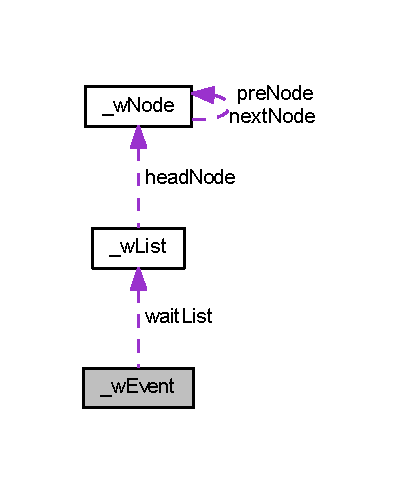
\includegraphics[width=192pt]{struct__w_event__coll__graph}
\end{center}
\end{figure}
\subsection*{成员变量}
\begin{DoxyCompactItemize}
\item 
\mbox{\hyperlink{w_event_8h_ab0672c982196a07535850096d01686c6}{w\+Event\+Type}} \mbox{\hyperlink{struct__w_event_ac98b322cb954407564af85e1cbfe18c2}{type}}
\item 
\mbox{\hyperlink{w_lib_8h_a3f922f977222a1e1fc18bd2ce6d668c3}{w\+List}} \mbox{\hyperlink{struct__w_event_a53d4661687eeb23d08fb0a94ef2918c3}{wait\+List}}
\end{DoxyCompactItemize}


\subsection{详细描述}
事件控制结构 

\subsection{结构体成员变量说明}
\mbox{\Hypertarget{struct__w_event_ac98b322cb954407564af85e1cbfe18c2}\label{struct__w_event_ac98b322cb954407564af85e1cbfe18c2}} 
\index{\+\_\+w\+Event@{\+\_\+w\+Event}!type@{type}}
\index{type@{type}!\+\_\+w\+Event@{\+\_\+w\+Event}}
\subsubsection{\texorpdfstring{type}{type}}
{\footnotesize\ttfamily \mbox{\hyperlink{w_event_8h_ab0672c982196a07535850096d01686c6}{w\+Event\+Type}} type}

Event类型 \mbox{\Hypertarget{struct__w_event_a53d4661687eeb23d08fb0a94ef2918c3}\label{struct__w_event_a53d4661687eeb23d08fb0a94ef2918c3}} 
\index{\+\_\+w\+Event@{\+\_\+w\+Event}!wait\+List@{wait\+List}}
\index{wait\+List@{wait\+List}!\+\_\+w\+Event@{\+\_\+w\+Event}}
\subsubsection{\texorpdfstring{wait\+List}{waitList}}
{\footnotesize\ttfamily \mbox{\hyperlink{w_lib_8h_a3f922f977222a1e1fc18bd2ce6d668c3}{w\+List}} wait\+List}

任务等待列表 

该结构体的文档由以下文件生成\+:\begin{DoxyCompactItemize}
\item 
C\+:/\+Users/pc/\+Desktop/\+W\+Q\+\_\+\+O\+S/\+Project/\+Sourse/\mbox{\hyperlink{w_event_8h}{w\+Event.\+h}}\end{DoxyCompactItemize}

\hypertarget{struct__w_flag_group}{}\section{\+\_\+w\+Flag\+Group结构体 参考}
\label{struct__w_flag_group}\index{\+\_\+w\+Flag\+Group@{\+\_\+w\+Flag\+Group}}


定义事件标志组类型  




{\ttfamily \#include $<$w\+Flag\+Group.\+h$>$}



\+\_\+w\+Flag\+Group 的协作图\+:
\nopagebreak
\begin{figure}[H]
\begin{center}
\leavevmode
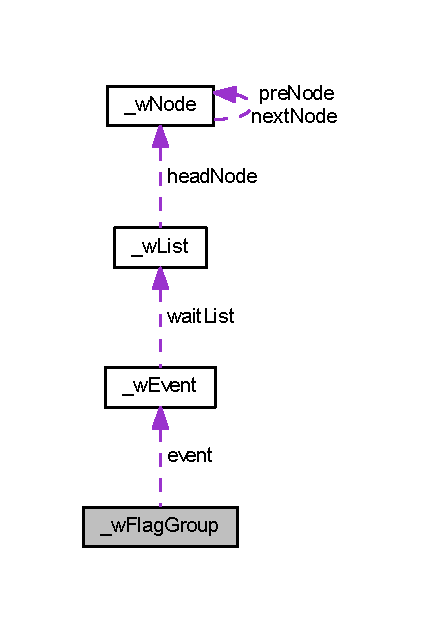
\includegraphics[width=203pt]{struct__w_flag_group__coll__graph}
\end{center}
\end{figure}
\subsection*{成员变量}
\begin{DoxyCompactItemize}
\item 
\mbox{\hyperlink{w_event_8h_af8b15988a26e1ac0d63eaf3fc5afe9d3}{w\+Event}} \mbox{\hyperlink{struct__w_flag_group_ad737d3f95a5cf9ee457f37f1cedfa44a}{event}}
\item 
uint32\+\_\+t \mbox{\hyperlink{struct__w_flag_group_a8fac2498fe5bd106b35d43af5bc91f6f}{flag}}
\end{DoxyCompactItemize}


\subsection{详细描述}
定义事件标志组类型 

\subsection{结构体成员变量说明}
\mbox{\Hypertarget{struct__w_flag_group_ad737d3f95a5cf9ee457f37f1cedfa44a}\label{struct__w_flag_group_ad737d3f95a5cf9ee457f37f1cedfa44a}} 
\index{\+\_\+w\+Flag\+Group@{\+\_\+w\+Flag\+Group}!event@{event}}
\index{event@{event}!\+\_\+w\+Flag\+Group@{\+\_\+w\+Flag\+Group}}
\subsubsection{\texorpdfstring{event}{event}}
{\footnotesize\ttfamily \mbox{\hyperlink{w_event_8h_af8b15988a26e1ac0d63eaf3fc5afe9d3}{w\+Event}} event}

事件控制块,w\+Flag\+Group同时是一个w\+Event \mbox{\Hypertarget{struct__w_flag_group_a8fac2498fe5bd106b35d43af5bc91f6f}\label{struct__w_flag_group_a8fac2498fe5bd106b35d43af5bc91f6f}} 
\index{\+\_\+w\+Flag\+Group@{\+\_\+w\+Flag\+Group}!flag@{flag}}
\index{flag@{flag}!\+\_\+w\+Flag\+Group@{\+\_\+w\+Flag\+Group}}
\subsubsection{\texorpdfstring{flag}{flag}}
{\footnotesize\ttfamily uint32\+\_\+t flag}

当前事件标志 

该结构体的文档由以下文件生成\+:\begin{DoxyCompactItemize}
\item 
C\+:/\+Users/pc/\+Desktop/\+W\+Q\+\_\+\+O\+S/\+Project/\+Sourse/\mbox{\hyperlink{w_flag_group_8h}{w\+Flag\+Group.\+h}}\end{DoxyCompactItemize}

\hypertarget{struct__w_flag_group_info}{}\section{\+\_\+w\+Flag\+Group\+Info结构体 参考}
\label{struct__w_flag_group_info}\index{\+\_\+w\+Flag\+Group\+Info@{\+\_\+w\+Flag\+Group\+Info}}


定义事件标志组信息结构  




{\ttfamily \#include $<$w\+Flag\+Group.\+h$>$}

\subsection*{成员变量}
\begin{DoxyCompactItemize}
\item 
uint32\+\_\+t \mbox{\hyperlink{struct__w_flag_group_info_a773b39d480759f67926cb18ae2219281}{flags}}
\item 
uint32\+\_\+t \mbox{\hyperlink{struct__w_flag_group_info_a80462c64b9184115aa568f08227f7f4a}{task\+Count}}
\end{DoxyCompactItemize}


\subsection{详细描述}
定义事件标志组信息结构 

\subsection{结构体成员变量说明}
\mbox{\Hypertarget{struct__w_flag_group_info_a773b39d480759f67926cb18ae2219281}\label{struct__w_flag_group_info_a773b39d480759f67926cb18ae2219281}} 
\index{\+\_\+w\+Flag\+Group\+Info@{\+\_\+w\+Flag\+Group\+Info}!flags@{flags}}
\index{flags@{flags}!\+\_\+w\+Flag\+Group\+Info@{\+\_\+w\+Flag\+Group\+Info}}
\subsubsection{\texorpdfstring{flags}{flags}}
{\footnotesize\ttfamily uint32\+\_\+t flags}

当前的事件标志 \mbox{\Hypertarget{struct__w_flag_group_info_a80462c64b9184115aa568f08227f7f4a}\label{struct__w_flag_group_info_a80462c64b9184115aa568f08227f7f4a}} 
\index{\+\_\+w\+Flag\+Group\+Info@{\+\_\+w\+Flag\+Group\+Info}!task\+Count@{task\+Count}}
\index{task\+Count@{task\+Count}!\+\_\+w\+Flag\+Group\+Info@{\+\_\+w\+Flag\+Group\+Info}}
\subsubsection{\texorpdfstring{task\+Count}{taskCount}}
{\footnotesize\ttfamily uint32\+\_\+t task\+Count}

当前等待的任务数 

该结构体的文档由以下文件生成\+:\begin{DoxyCompactItemize}
\item 
C\+:/\+Users/pc/\+Desktop/\+W\+Q\+\_\+\+O\+S/\+Project/\+Sourse/\mbox{\hyperlink{w_flag_group_8h}{w\+Flag\+Group.\+h}}\end{DoxyCompactItemize}

\hypertarget{struct__w_list}{}\section{\+\_\+w\+List结构体 参考}
\label{struct__w_list}\index{\+\_\+w\+List@{\+\_\+w\+List}}


链表结构体  




{\ttfamily \#include $<$w\+Lib.\+h$>$}



\+\_\+w\+List 的协作图\+:
\nopagebreak
\begin{figure}[H]
\begin{center}
\leavevmode
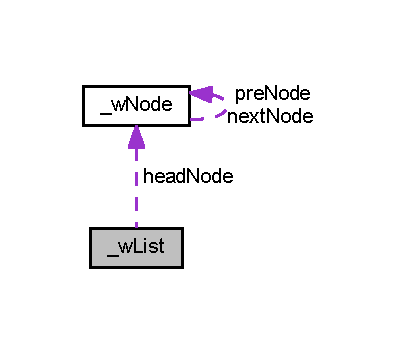
\includegraphics[width=191pt]{struct__w_list__coll__graph}
\end{center}
\end{figure}
\subsection*{成员变量}
\begin{DoxyCompactItemize}
\item 
\mbox{\hyperlink{w_lib_8h_a98363f2fc9ff1bef5993786140d900f2}{w\+Node}} \mbox{\hyperlink{struct__w_list_a306555352c507bb9f10c507680666624}{head\+Node}}
\item 
uint32\+\_\+t \mbox{\hyperlink{struct__w_list_a9ff3c0ff509d8eb055d29faa0ec185a1}{node\+Count}}
\end{DoxyCompactItemize}


\subsection{详细描述}
链表结构体 

\subsection{结构体成员变量说明}
\mbox{\Hypertarget{struct__w_list_a306555352c507bb9f10c507680666624}\label{struct__w_list_a306555352c507bb9f10c507680666624}} 
\index{\+\_\+w\+List@{\+\_\+w\+List}!head\+Node@{head\+Node}}
\index{head\+Node@{head\+Node}!\+\_\+w\+List@{\+\_\+w\+List}}
\subsubsection{\texorpdfstring{head\+Node}{headNode}}
{\footnotesize\ttfamily \mbox{\hyperlink{w_lib_8h_a98363f2fc9ff1bef5993786140d900f2}{w\+Node}} head\+Node}

\mbox{\Hypertarget{struct__w_list_a9ff3c0ff509d8eb055d29faa0ec185a1}\label{struct__w_list_a9ff3c0ff509d8eb055d29faa0ec185a1}} 
\index{\+\_\+w\+List@{\+\_\+w\+List}!node\+Count@{node\+Count}}
\index{node\+Count@{node\+Count}!\+\_\+w\+List@{\+\_\+w\+List}}
\subsubsection{\texorpdfstring{node\+Count}{nodeCount}}
{\footnotesize\ttfamily uint32\+\_\+t node\+Count}



该结构体的文档由以下文件生成\+:\begin{DoxyCompactItemize}
\item 
C\+:/\+Users/pc/\+Desktop/\+W\+Q\+\_\+\+O\+S/\+Project/\+Sourse/\mbox{\hyperlink{w_lib_8h}{w\+Lib.\+h}}\end{DoxyCompactItemize}

\hypertarget{struct__w_mbox}{}\section{\+\_\+w\+Mbox结构体 参考}
\label{struct__w_mbox}\index{\+\_\+w\+Mbox@{\+\_\+w\+Mbox}}


定义邮箱类型  




{\ttfamily \#include $<$w\+Mbox.\+h$>$}



\+\_\+w\+Mbox 的协作图\+:
\nopagebreak
\begin{figure}[H]
\begin{center}
\leavevmode
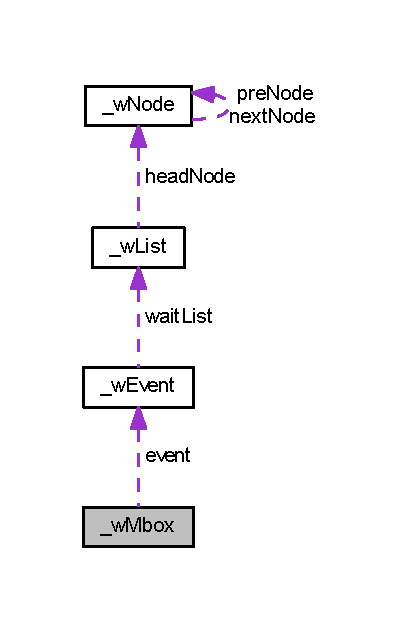
\includegraphics[width=192pt]{struct__w_mbox__coll__graph}
\end{center}
\end{figure}
\subsection*{成员变量}
\begin{DoxyCompactItemize}
\item 
\mbox{\hyperlink{w_event_8h_af8b15988a26e1ac0d63eaf3fc5afe9d3}{w\+Event}} \mbox{\hyperlink{struct__w_mbox_ad737d3f95a5cf9ee457f37f1cedfa44a}{event}}
\item 
uint32\+\_\+t \mbox{\hyperlink{struct__w_mbox_a86988a65e0d3ece7990c032c159786d6}{count}}
\item 
uint32\+\_\+t \mbox{\hyperlink{struct__w_mbox_a0a71cf941cf2509857d61e1443ad8eaa}{read}}
\item 
uint32\+\_\+t \mbox{\hyperlink{struct__w_mbox_ac4c9f9c5eac363cc22ecc18669cc3891}{write}}
\item 
uint32\+\_\+t \mbox{\hyperlink{struct__w_mbox_a1cc8a4ba5eee24b560f9869012941e91}{max\+Count}}
\item 
void $\ast$$\ast$ \mbox{\hyperlink{struct__w_mbox_a42b4bab76140c12b77b72ec381001c6c}{msg\+Buffer}}
\end{DoxyCompactItemize}


\subsection{详细描述}
定义邮箱类型 

\subsection{结构体成员变量说明}
\mbox{\Hypertarget{struct__w_mbox_a86988a65e0d3ece7990c032c159786d6}\label{struct__w_mbox_a86988a65e0d3ece7990c032c159786d6}} 
\index{\+\_\+w\+Mbox@{\+\_\+w\+Mbox}!count@{count}}
\index{count@{count}!\+\_\+w\+Mbox@{\+\_\+w\+Mbox}}
\subsubsection{\texorpdfstring{count}{count}}
{\footnotesize\ttfamily uint32\+\_\+t count}

当前消息数 \mbox{\Hypertarget{struct__w_mbox_ad737d3f95a5cf9ee457f37f1cedfa44a}\label{struct__w_mbox_ad737d3f95a5cf9ee457f37f1cedfa44a}} 
\index{\+\_\+w\+Mbox@{\+\_\+w\+Mbox}!event@{event}}
\index{event@{event}!\+\_\+w\+Mbox@{\+\_\+w\+Mbox}}
\subsubsection{\texorpdfstring{event}{event}}
{\footnotesize\ttfamily \mbox{\hyperlink{w_event_8h_af8b15988a26e1ac0d63eaf3fc5afe9d3}{w\+Event}} event}

事件控制块,w\+Mbox同时是一个w\+Event \mbox{\Hypertarget{struct__w_mbox_a1cc8a4ba5eee24b560f9869012941e91}\label{struct__w_mbox_a1cc8a4ba5eee24b560f9869012941e91}} 
\index{\+\_\+w\+Mbox@{\+\_\+w\+Mbox}!max\+Count@{max\+Count}}
\index{max\+Count@{max\+Count}!\+\_\+w\+Mbox@{\+\_\+w\+Mbox}}
\subsubsection{\texorpdfstring{max\+Count}{maxCount}}
{\footnotesize\ttfamily uint32\+\_\+t max\+Count}

最大消息数 \mbox{\Hypertarget{struct__w_mbox_a42b4bab76140c12b77b72ec381001c6c}\label{struct__w_mbox_a42b4bab76140c12b77b72ec381001c6c}} 
\index{\+\_\+w\+Mbox@{\+\_\+w\+Mbox}!msg\+Buffer@{msg\+Buffer}}
\index{msg\+Buffer@{msg\+Buffer}!\+\_\+w\+Mbox@{\+\_\+w\+Mbox}}
\subsubsection{\texorpdfstring{msg\+Buffer}{msgBuffer}}
{\footnotesize\ttfamily void$\ast$$\ast$ msg\+Buffer}

消息存储缓冲区 \mbox{\Hypertarget{struct__w_mbox_a0a71cf941cf2509857d61e1443ad8eaa}\label{struct__w_mbox_a0a71cf941cf2509857d61e1443ad8eaa}} 
\index{\+\_\+w\+Mbox@{\+\_\+w\+Mbox}!read@{read}}
\index{read@{read}!\+\_\+w\+Mbox@{\+\_\+w\+Mbox}}
\subsubsection{\texorpdfstring{read}{read}}
{\footnotesize\ttfamily uint32\+\_\+t read}

读索引 \mbox{\Hypertarget{struct__w_mbox_ac4c9f9c5eac363cc22ecc18669cc3891}\label{struct__w_mbox_ac4c9f9c5eac363cc22ecc18669cc3891}} 
\index{\+\_\+w\+Mbox@{\+\_\+w\+Mbox}!write@{write}}
\index{write@{write}!\+\_\+w\+Mbox@{\+\_\+w\+Mbox}}
\subsubsection{\texorpdfstring{write}{write}}
{\footnotesize\ttfamily uint32\+\_\+t write}

写索引 

该结构体的文档由以下文件生成\+:\begin{DoxyCompactItemize}
\item 
C\+:/\+Users/pc/\+Desktop/\+W\+Q\+\_\+\+O\+S/\+Project/\+Sourse/\mbox{\hyperlink{w_mbox_8h}{w\+Mbox.\+h}}\end{DoxyCompactItemize}

\hypertarget{struct__w_mbox_info}{}\section{\+\_\+w\+Mbox\+Info结构体 参考}
\label{struct__w_mbox_info}\index{\+\_\+w\+Mbox\+Info@{\+\_\+w\+Mbox\+Info}}


定义邮箱信息结构  




{\ttfamily \#include $<$w\+Mbox.\+h$>$}

\subsection*{成员变量}
\begin{DoxyCompactItemize}
\item 
uint32\+\_\+t \mbox{\hyperlink{struct__w_mbox_info_a86988a65e0d3ece7990c032c159786d6}{count}}
\item 
uint32\+\_\+t \mbox{\hyperlink{struct__w_mbox_info_a1cc8a4ba5eee24b560f9869012941e91}{max\+Count}}
\item 
uint32\+\_\+t \mbox{\hyperlink{struct__w_mbox_info_a80462c64b9184115aa568f08227f7f4a}{task\+Count}}
\end{DoxyCompactItemize}


\subsection{详细描述}
定义邮箱信息结构 

\subsection{结构体成员变量说明}
\mbox{\Hypertarget{struct__w_mbox_info_a86988a65e0d3ece7990c032c159786d6}\label{struct__w_mbox_info_a86988a65e0d3ece7990c032c159786d6}} 
\index{\+\_\+w\+Mbox\+Info@{\+\_\+w\+Mbox\+Info}!count@{count}}
\index{count@{count}!\+\_\+w\+Mbox\+Info@{\+\_\+w\+Mbox\+Info}}
\subsubsection{\texorpdfstring{count}{count}}
{\footnotesize\ttfamily uint32\+\_\+t count}

当前消息数 \mbox{\Hypertarget{struct__w_mbox_info_a1cc8a4ba5eee24b560f9869012941e91}\label{struct__w_mbox_info_a1cc8a4ba5eee24b560f9869012941e91}} 
\index{\+\_\+w\+Mbox\+Info@{\+\_\+w\+Mbox\+Info}!max\+Count@{max\+Count}}
\index{max\+Count@{max\+Count}!\+\_\+w\+Mbox\+Info@{\+\_\+w\+Mbox\+Info}}
\subsubsection{\texorpdfstring{max\+Count}{maxCount}}
{\footnotesize\ttfamily uint32\+\_\+t max\+Count}

最大消息数 \mbox{\Hypertarget{struct__w_mbox_info_a80462c64b9184115aa568f08227f7f4a}\label{struct__w_mbox_info_a80462c64b9184115aa568f08227f7f4a}} 
\index{\+\_\+w\+Mbox\+Info@{\+\_\+w\+Mbox\+Info}!task\+Count@{task\+Count}}
\index{task\+Count@{task\+Count}!\+\_\+w\+Mbox\+Info@{\+\_\+w\+Mbox\+Info}}
\subsubsection{\texorpdfstring{task\+Count}{taskCount}}
{\footnotesize\ttfamily uint32\+\_\+t task\+Count}

等待的任务数 

该结构体的文档由以下文件生成\+:\begin{DoxyCompactItemize}
\item 
C\+:/\+Users/pc/\+Desktop/\+W\+Q\+\_\+\+O\+S/\+Project/\+Sourse/\mbox{\hyperlink{w_mbox_8h}{w\+Mbox.\+h}}\end{DoxyCompactItemize}

\hypertarget{struct__w_mem_block}{}\section{\+\_\+w\+Mem\+Block结构体 参考}
\label{struct__w_mem_block}\index{\+\_\+w\+Mem\+Block@{\+\_\+w\+Mem\+Block}}


定义存储块类型  




{\ttfamily \#include $<$w\+Mem\+Block.\+h$>$}



\+\_\+w\+Mem\+Block 的协作图\+:
\nopagebreak
\begin{figure}[H]
\begin{center}
\leavevmode
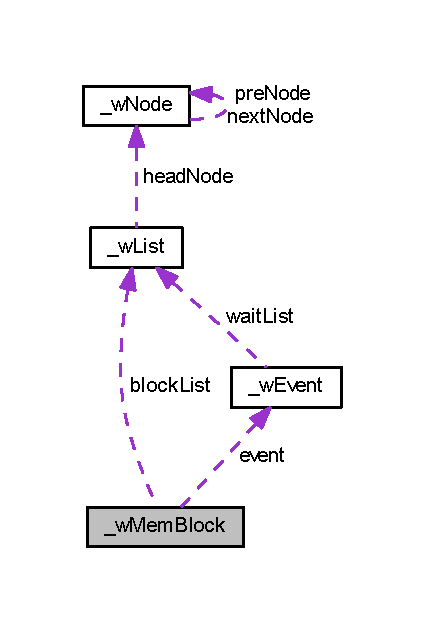
\includegraphics[width=204pt]{struct__w_mem_block__coll__graph}
\end{center}
\end{figure}
\subsection*{成员变量}
\begin{DoxyCompactItemize}
\item 
\mbox{\hyperlink{w_event_8h_af8b15988a26e1ac0d63eaf3fc5afe9d3}{w\+Event}} \mbox{\hyperlink{struct__w_mem_block_ad737d3f95a5cf9ee457f37f1cedfa44a}{event}}
\item 
void $\ast$ \mbox{\hyperlink{struct__w_mem_block_a278e5d28605731490bb61cb8d313a5f3}{mem\+Start}}
\item 
uint32\+\_\+t \mbox{\hyperlink{struct__w_mem_block_ab6558f40a619c2502fbc24c880fd4fb0}{block\+Size}}
\item 
uint32\+\_\+t \mbox{\hyperlink{struct__w_mem_block_a1cc8a4ba5eee24b560f9869012941e91}{max\+Count}}
\item 
\mbox{\hyperlink{w_lib_8h_a3f922f977222a1e1fc18bd2ce6d668c3}{w\+List}} \mbox{\hyperlink{struct__w_mem_block_a2247091b4ceb8f63ff199b551bb3c352}{block\+List}}
\end{DoxyCompactItemize}


\subsection{详细描述}
定义存储块类型 

\subsection{结构体成员变量说明}
\mbox{\Hypertarget{struct__w_mem_block_a2247091b4ceb8f63ff199b551bb3c352}\label{struct__w_mem_block_a2247091b4ceb8f63ff199b551bb3c352}} 
\index{\+\_\+w\+Mem\+Block@{\+\_\+w\+Mem\+Block}!block\+List@{block\+List}}
\index{block\+List@{block\+List}!\+\_\+w\+Mem\+Block@{\+\_\+w\+Mem\+Block}}
\subsubsection{\texorpdfstring{block\+List}{blockList}}
{\footnotesize\ttfamily \mbox{\hyperlink{w_lib_8h_a3f922f977222a1e1fc18bd2ce6d668c3}{w\+List}} block\+List}

存储块链表 \mbox{\Hypertarget{struct__w_mem_block_ab6558f40a619c2502fbc24c880fd4fb0}\label{struct__w_mem_block_ab6558f40a619c2502fbc24c880fd4fb0}} 
\index{\+\_\+w\+Mem\+Block@{\+\_\+w\+Mem\+Block}!block\+Size@{block\+Size}}
\index{block\+Size@{block\+Size}!\+\_\+w\+Mem\+Block@{\+\_\+w\+Mem\+Block}}
\subsubsection{\texorpdfstring{block\+Size}{blockSize}}
{\footnotesize\ttfamily uint32\+\_\+t block\+Size}

存储块大小 \mbox{\Hypertarget{struct__w_mem_block_ad737d3f95a5cf9ee457f37f1cedfa44a}\label{struct__w_mem_block_ad737d3f95a5cf9ee457f37f1cedfa44a}} 
\index{\+\_\+w\+Mem\+Block@{\+\_\+w\+Mem\+Block}!event@{event}}
\index{event@{event}!\+\_\+w\+Mem\+Block@{\+\_\+w\+Mem\+Block}}
\subsubsection{\texorpdfstring{event}{event}}
{\footnotesize\ttfamily \mbox{\hyperlink{w_event_8h_af8b15988a26e1ac0d63eaf3fc5afe9d3}{w\+Event}} event}

事件控制块,w\+Mem\+Block同时是一个w\+Event \mbox{\Hypertarget{struct__w_mem_block_a1cc8a4ba5eee24b560f9869012941e91}\label{struct__w_mem_block_a1cc8a4ba5eee24b560f9869012941e91}} 
\index{\+\_\+w\+Mem\+Block@{\+\_\+w\+Mem\+Block}!max\+Count@{max\+Count}}
\index{max\+Count@{max\+Count}!\+\_\+w\+Mem\+Block@{\+\_\+w\+Mem\+Block}}
\subsubsection{\texorpdfstring{max\+Count}{maxCount}}
{\footnotesize\ttfamily uint32\+\_\+t max\+Count}

存储块最大个数 \mbox{\Hypertarget{struct__w_mem_block_a278e5d28605731490bb61cb8d313a5f3}\label{struct__w_mem_block_a278e5d28605731490bb61cb8d313a5f3}} 
\index{\+\_\+w\+Mem\+Block@{\+\_\+w\+Mem\+Block}!mem\+Start@{mem\+Start}}
\index{mem\+Start@{mem\+Start}!\+\_\+w\+Mem\+Block@{\+\_\+w\+Mem\+Block}}
\subsubsection{\texorpdfstring{mem\+Start}{memStart}}
{\footnotesize\ttfamily void$\ast$ mem\+Start}

存储块首地址 

该结构体的文档由以下文件生成\+:\begin{DoxyCompactItemize}
\item 
C\+:/\+Users/pc/\+Desktop/\+W\+Q\+\_\+\+O\+S/\+Project/\+Sourse/\mbox{\hyperlink{w_mem_block_8h}{w\+Mem\+Block.\+h}}\end{DoxyCompactItemize}

\hypertarget{struct__w_mem_block_info}{}\section{\+\_\+w\+Mem\+Block\+Info结构体 参考}
\label{struct__w_mem_block_info}\index{\+\_\+w\+Mem\+Block\+Info@{\+\_\+w\+Mem\+Block\+Info}}


定义存储块信息结构  




{\ttfamily \#include $<$w\+Mem\+Block.\+h$>$}

\subsection*{成员变量}
\begin{DoxyCompactItemize}
\item 
uint32\+\_\+t \mbox{\hyperlink{struct__w_mem_block_info_a86988a65e0d3ece7990c032c159786d6}{count}}
\item 
uint32\+\_\+t \mbox{\hyperlink{struct__w_mem_block_info_a1cc8a4ba5eee24b560f9869012941e91}{max\+Count}}
\item 
uint32\+\_\+t \mbox{\hyperlink{struct__w_mem_block_info_ab6558f40a619c2502fbc24c880fd4fb0}{block\+Size}}
\item 
uint32\+\_\+t \mbox{\hyperlink{struct__w_mem_block_info_a80462c64b9184115aa568f08227f7f4a}{task\+Count}}
\end{DoxyCompactItemize}


\subsection{详细描述}
定义存储块信息结构 

\subsection{结构体成员变量说明}
\mbox{\Hypertarget{struct__w_mem_block_info_ab6558f40a619c2502fbc24c880fd4fb0}\label{struct__w_mem_block_info_ab6558f40a619c2502fbc24c880fd4fb0}} 
\index{\+\_\+w\+Mem\+Block\+Info@{\+\_\+w\+Mem\+Block\+Info}!block\+Size@{block\+Size}}
\index{block\+Size@{block\+Size}!\+\_\+w\+Mem\+Block\+Info@{\+\_\+w\+Mem\+Block\+Info}}
\subsubsection{\texorpdfstring{block\+Size}{blockSize}}
{\footnotesize\ttfamily uint32\+\_\+t block\+Size}

每个存储块的大小 \mbox{\Hypertarget{struct__w_mem_block_info_a86988a65e0d3ece7990c032c159786d6}\label{struct__w_mem_block_info_a86988a65e0d3ece7990c032c159786d6}} 
\index{\+\_\+w\+Mem\+Block\+Info@{\+\_\+w\+Mem\+Block\+Info}!count@{count}}
\index{count@{count}!\+\_\+w\+Mem\+Block\+Info@{\+\_\+w\+Mem\+Block\+Info}}
\subsubsection{\texorpdfstring{count}{count}}
{\footnotesize\ttfamily uint32\+\_\+t count}

当前存储块的计数 \mbox{\Hypertarget{struct__w_mem_block_info_a1cc8a4ba5eee24b560f9869012941e91}\label{struct__w_mem_block_info_a1cc8a4ba5eee24b560f9869012941e91}} 
\index{\+\_\+w\+Mem\+Block\+Info@{\+\_\+w\+Mem\+Block\+Info}!max\+Count@{max\+Count}}
\index{max\+Count@{max\+Count}!\+\_\+w\+Mem\+Block\+Info@{\+\_\+w\+Mem\+Block\+Info}}
\subsubsection{\texorpdfstring{max\+Count}{maxCount}}
{\footnotesize\ttfamily uint32\+\_\+t max\+Count}

允许的存储块最大计数 \mbox{\Hypertarget{struct__w_mem_block_info_a80462c64b9184115aa568f08227f7f4a}\label{struct__w_mem_block_info_a80462c64b9184115aa568f08227f7f4a}} 
\index{\+\_\+w\+Mem\+Block\+Info@{\+\_\+w\+Mem\+Block\+Info}!task\+Count@{task\+Count}}
\index{task\+Count@{task\+Count}!\+\_\+w\+Mem\+Block\+Info@{\+\_\+w\+Mem\+Block\+Info}}
\subsubsection{\texorpdfstring{task\+Count}{taskCount}}
{\footnotesize\ttfamily uint32\+\_\+t task\+Count}

当前等待的任务计数 

该结构体的文档由以下文件生成\+:\begin{DoxyCompactItemize}
\item 
C\+:/\+Users/pc/\+Desktop/\+W\+Q\+\_\+\+O\+S/\+Project/\+Sourse/\mbox{\hyperlink{w_mem_block_8h}{w\+Mem\+Block.\+h}}\end{DoxyCompactItemize}

\hypertarget{struct__w_mutex}{}\section{\+\_\+w\+Mutex结构体 参考}
\label{struct__w_mutex}\index{\+\_\+w\+Mutex@{\+\_\+w\+Mutex}}


定义互斥信号量类型  




{\ttfamily \#include $<$w\+Mutex.\+h$>$}



\+\_\+w\+Mutex 的协作图\+:
\nopagebreak
\begin{figure}[H]
\begin{center}
\leavevmode
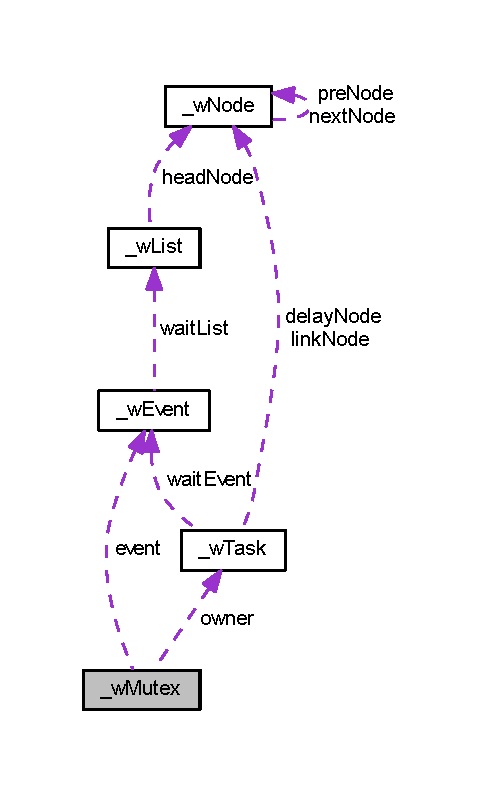
\includegraphics[width=231pt]{struct__w_mutex__coll__graph}
\end{center}
\end{figure}
\subsection*{成员变量}
\begin{DoxyCompactItemize}
\item 
\mbox{\hyperlink{w_event_8h_af8b15988a26e1ac0d63eaf3fc5afe9d3}{w\+Event}} \mbox{\hyperlink{struct__w_mutex_ad737d3f95a5cf9ee457f37f1cedfa44a}{event}}
\item 
uint32\+\_\+t \mbox{\hyperlink{struct__w_mutex_a16598f387191bb413e5c802b23e501ef}{locked\+Count}}
\item 
\mbox{\hyperlink{w_task_8h_acd0e6238476f631a6ac4588629bac372}{w\+Task}} $\ast$ \mbox{\hyperlink{struct__w_mutex_a1ed47712ef6760f64988107466c22321}{owner}}
\item 
uint32\+\_\+t \mbox{\hyperlink{struct__w_mutex_aa1d8803bb70576a417cba7092640ebd3}{owner\+Original\+Prio}}
\end{DoxyCompactItemize}


\subsection{详细描述}
定义互斥信号量类型 

\subsection{结构体成员变量说明}
\mbox{\Hypertarget{struct__w_mutex_ad737d3f95a5cf9ee457f37f1cedfa44a}\label{struct__w_mutex_ad737d3f95a5cf9ee457f37f1cedfa44a}} 
\index{\+\_\+w\+Mutex@{\+\_\+w\+Mutex}!event@{event}}
\index{event@{event}!\+\_\+w\+Mutex@{\+\_\+w\+Mutex}}
\subsubsection{\texorpdfstring{event}{event}}
{\footnotesize\ttfamily \mbox{\hyperlink{w_event_8h_af8b15988a26e1ac0d63eaf3fc5afe9d3}{w\+Event}} event}

事件控制块,w\+Mutex同时是一个w\+Event \mbox{\Hypertarget{struct__w_mutex_a16598f387191bb413e5c802b23e501ef}\label{struct__w_mutex_a16598f387191bb413e5c802b23e501ef}} 
\index{\+\_\+w\+Mutex@{\+\_\+w\+Mutex}!locked\+Count@{locked\+Count}}
\index{locked\+Count@{locked\+Count}!\+\_\+w\+Mutex@{\+\_\+w\+Mutex}}
\subsubsection{\texorpdfstring{locked\+Count}{lockedCount}}
{\footnotesize\ttfamily uint32\+\_\+t locked\+Count}

已被锁定的次数 \mbox{\Hypertarget{struct__w_mutex_a1ed47712ef6760f64988107466c22321}\label{struct__w_mutex_a1ed47712ef6760f64988107466c22321}} 
\index{\+\_\+w\+Mutex@{\+\_\+w\+Mutex}!owner@{owner}}
\index{owner@{owner}!\+\_\+w\+Mutex@{\+\_\+w\+Mutex}}
\subsubsection{\texorpdfstring{owner}{owner}}
{\footnotesize\ttfamily \mbox{\hyperlink{w_task_8h_acd0e6238476f631a6ac4588629bac372}{w\+Task}}$\ast$ owner}

拥有者 \mbox{\Hypertarget{struct__w_mutex_aa1d8803bb70576a417cba7092640ebd3}\label{struct__w_mutex_aa1d8803bb70576a417cba7092640ebd3}} 
\index{\+\_\+w\+Mutex@{\+\_\+w\+Mutex}!owner\+Original\+Prio@{owner\+Original\+Prio}}
\index{owner\+Original\+Prio@{owner\+Original\+Prio}!\+\_\+w\+Mutex@{\+\_\+w\+Mutex}}
\subsubsection{\texorpdfstring{owner\+Original\+Prio}{ownerOriginalPrio}}
{\footnotesize\ttfamily uint32\+\_\+t owner\+Original\+Prio}

拥有者原始的优先级 

该结构体的文档由以下文件生成\+:\begin{DoxyCompactItemize}
\item 
C\+:/\+Users/pc/\+Desktop/\+W\+Q\+\_\+\+O\+S/\+Project/\+Sourse/\mbox{\hyperlink{w_mutex_8h}{w\+Mutex.\+h}}\end{DoxyCompactItemize}

\hypertarget{struct__w_mutex_info}{}\section{\+\_\+w\+Mutex\+Info结构体 参考}
\label{struct__w_mutex_info}\index{\+\_\+w\+Mutex\+Info@{\+\_\+w\+Mutex\+Info}}


定义互斥信号量信息结构  




{\ttfamily \#include $<$w\+Mutex.\+h$>$}



\+\_\+w\+Mutex\+Info 的协作图\+:
\nopagebreak
\begin{figure}[H]
\begin{center}
\leavevmode
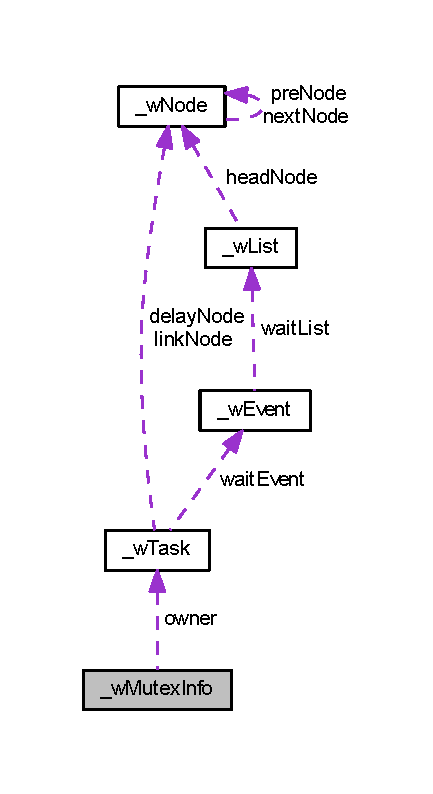
\includegraphics[width=208pt]{struct__w_mutex_info__coll__graph}
\end{center}
\end{figure}
\subsection*{成员变量}
\begin{DoxyCompactItemize}
\item 
uint32\+\_\+t \mbox{\hyperlink{struct__w_mutex_info_a80462c64b9184115aa568f08227f7f4a}{task\+Count}}
\item 
uint32\+\_\+t \mbox{\hyperlink{struct__w_mutex_info_a2ad329dc18ddf3afd170e73535c5907a}{owner\+Prio}}
\item 
uint32\+\_\+t \mbox{\hyperlink{struct__w_mutex_info_ad2ca878c1d7b4012ae3954a79aa664ef}{inherited\+Prio}}
\item 
\mbox{\hyperlink{w_task_8h_acd0e6238476f631a6ac4588629bac372}{w\+Task}} $\ast$ \mbox{\hyperlink{struct__w_mutex_info_a1ed47712ef6760f64988107466c22321}{owner}}
\item 
uint32\+\_\+t \mbox{\hyperlink{struct__w_mutex_info_a16598f387191bb413e5c802b23e501ef}{locked\+Count}}
\end{DoxyCompactItemize}


\subsection{详细描述}
定义互斥信号量信息结构 

\subsection{结构体成员变量说明}
\mbox{\Hypertarget{struct__w_mutex_info_ad2ca878c1d7b4012ae3954a79aa664ef}\label{struct__w_mutex_info_ad2ca878c1d7b4012ae3954a79aa664ef}} 
\index{\+\_\+w\+Mutex\+Info@{\+\_\+w\+Mutex\+Info}!inherited\+Prio@{inherited\+Prio}}
\index{inherited\+Prio@{inherited\+Prio}!\+\_\+w\+Mutex\+Info@{\+\_\+w\+Mutex\+Info}}
\subsubsection{\texorpdfstring{inherited\+Prio}{inheritedPrio}}
{\footnotesize\ttfamily uint32\+\_\+t inherited\+Prio}

继承者优先级 \mbox{\Hypertarget{struct__w_mutex_info_a16598f387191bb413e5c802b23e501ef}\label{struct__w_mutex_info_a16598f387191bb413e5c802b23e501ef}} 
\index{\+\_\+w\+Mutex\+Info@{\+\_\+w\+Mutex\+Info}!locked\+Count@{locked\+Count}}
\index{locked\+Count@{locked\+Count}!\+\_\+w\+Mutex\+Info@{\+\_\+w\+Mutex\+Info}}
\subsubsection{\texorpdfstring{locked\+Count}{lockedCount}}
{\footnotesize\ttfamily uint32\+\_\+t locked\+Count}

锁定次数 \mbox{\Hypertarget{struct__w_mutex_info_a1ed47712ef6760f64988107466c22321}\label{struct__w_mutex_info_a1ed47712ef6760f64988107466c22321}} 
\index{\+\_\+w\+Mutex\+Info@{\+\_\+w\+Mutex\+Info}!owner@{owner}}
\index{owner@{owner}!\+\_\+w\+Mutex\+Info@{\+\_\+w\+Mutex\+Info}}
\subsubsection{\texorpdfstring{owner}{owner}}
{\footnotesize\ttfamily \mbox{\hyperlink{w_task_8h_acd0e6238476f631a6ac4588629bac372}{w\+Task}}$\ast$ owner}

拥有者 \mbox{\Hypertarget{struct__w_mutex_info_a2ad329dc18ddf3afd170e73535c5907a}\label{struct__w_mutex_info_a2ad329dc18ddf3afd170e73535c5907a}} 
\index{\+\_\+w\+Mutex\+Info@{\+\_\+w\+Mutex\+Info}!owner\+Prio@{owner\+Prio}}
\index{owner\+Prio@{owner\+Prio}!\+\_\+w\+Mutex\+Info@{\+\_\+w\+Mutex\+Info}}
\subsubsection{\texorpdfstring{owner\+Prio}{ownerPrio}}
{\footnotesize\ttfamily uint32\+\_\+t owner\+Prio}

拥有者原始优先级 \mbox{\Hypertarget{struct__w_mutex_info_a80462c64b9184115aa568f08227f7f4a}\label{struct__w_mutex_info_a80462c64b9184115aa568f08227f7f4a}} 
\index{\+\_\+w\+Mutex\+Info@{\+\_\+w\+Mutex\+Info}!task\+Count@{task\+Count}}
\index{task\+Count@{task\+Count}!\+\_\+w\+Mutex\+Info@{\+\_\+w\+Mutex\+Info}}
\subsubsection{\texorpdfstring{task\+Count}{taskCount}}
{\footnotesize\ttfamily uint32\+\_\+t task\+Count}

等待的任务数量 

该结构体的文档由以下文件生成\+:\begin{DoxyCompactItemize}
\item 
C\+:/\+Users/pc/\+Desktop/\+W\+Q\+\_\+\+O\+S/\+Project/\+Sourse/\mbox{\hyperlink{w_mutex_8h}{w\+Mutex.\+h}}\end{DoxyCompactItemize}

\hypertarget{struct__w_node}{}\section{\+\_\+w\+Node结构体 参考}
\label{struct__w_node}\index{\+\_\+w\+Node@{\+\_\+w\+Node}}


结点结构体  




{\ttfamily \#include $<$w\+Lib.\+h$>$}



\+\_\+w\+Node 的协作图\+:
\nopagebreak
\begin{figure}[H]
\begin{center}
\leavevmode
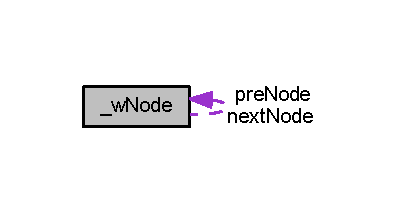
\includegraphics[width=191pt]{struct__w_node__coll__graph}
\end{center}
\end{figure}
\subsection*{成员变量}
\begin{DoxyCompactItemize}
\item 
struct \mbox{\hyperlink{struct__w_node}{\+\_\+w\+Node}} $\ast$ \mbox{\hyperlink{struct__w_node_abc26422bd712b569f20f912470cdca6d}{pre\+Node}}
\item 
struct \mbox{\hyperlink{struct__w_node}{\+\_\+w\+Node}} $\ast$ \mbox{\hyperlink{struct__w_node_a5a117484843cbaec00be972bb97d0752}{next\+Node}}
\end{DoxyCompactItemize}


\subsection{详细描述}
结点结构体 

\subsection{结构体成员变量说明}
\mbox{\Hypertarget{struct__w_node_a5a117484843cbaec00be972bb97d0752}\label{struct__w_node_a5a117484843cbaec00be972bb97d0752}} 
\index{\+\_\+w\+Node@{\+\_\+w\+Node}!next\+Node@{next\+Node}}
\index{next\+Node@{next\+Node}!\+\_\+w\+Node@{\+\_\+w\+Node}}
\subsubsection{\texorpdfstring{next\+Node}{nextNode}}
{\footnotesize\ttfamily struct \mbox{\hyperlink{struct__w_node}{\+\_\+w\+Node}}$\ast$ next\+Node}

\mbox{\Hypertarget{struct__w_node_abc26422bd712b569f20f912470cdca6d}\label{struct__w_node_abc26422bd712b569f20f912470cdca6d}} 
\index{\+\_\+w\+Node@{\+\_\+w\+Node}!pre\+Node@{pre\+Node}}
\index{pre\+Node@{pre\+Node}!\+\_\+w\+Node@{\+\_\+w\+Node}}
\subsubsection{\texorpdfstring{pre\+Node}{preNode}}
{\footnotesize\ttfamily struct \mbox{\hyperlink{struct__w_node}{\+\_\+w\+Node}}$\ast$ pre\+Node}



该结构体的文档由以下文件生成\+:\begin{DoxyCompactItemize}
\item 
C\+:/\+Users/pc/\+Desktop/\+W\+Q\+\_\+\+O\+S/\+Project/\+Sourse/\mbox{\hyperlink{w_lib_8h}{w\+Lib.\+h}}\end{DoxyCompactItemize}

\hypertarget{struct__w_sem}{}\section{\+\_\+w\+Sem结构体 参考}
\label{struct__w_sem}\index{\+\_\+w\+Sem@{\+\_\+w\+Sem}}


定义信号量类型  




{\ttfamily \#include $<$w\+Sem.\+h$>$}



\+\_\+w\+Sem 的协作图\+:
\nopagebreak
\begin{figure}[H]
\begin{center}
\leavevmode
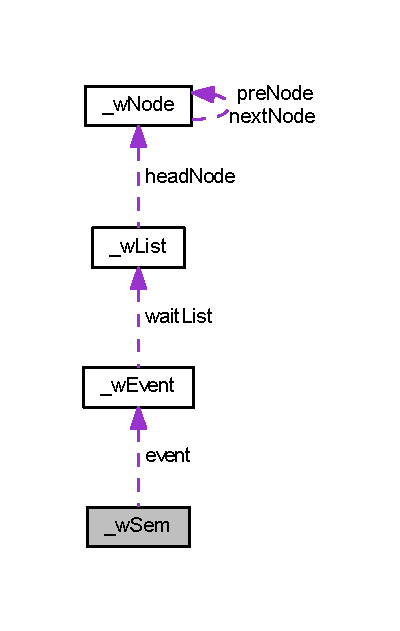
\includegraphics[width=192pt]{struct__w_sem__coll__graph}
\end{center}
\end{figure}
\subsection*{成员变量}
\begin{DoxyCompactItemize}
\item 
\mbox{\hyperlink{w_event_8h_af8b15988a26e1ac0d63eaf3fc5afe9d3}{w\+Event}} \mbox{\hyperlink{struct__w_sem_ad737d3f95a5cf9ee457f37f1cedfa44a}{event}}
\item 
uint32\+\_\+t \mbox{\hyperlink{struct__w_sem_a86988a65e0d3ece7990c032c159786d6}{count}}
\item 
uint32\+\_\+t \mbox{\hyperlink{struct__w_sem_a1cc8a4ba5eee24b560f9869012941e91}{max\+Count}}
\end{DoxyCompactItemize}


\subsection{详细描述}
定义信号量类型 

\subsection{结构体成员变量说明}
\mbox{\Hypertarget{struct__w_sem_a86988a65e0d3ece7990c032c159786d6}\label{struct__w_sem_a86988a65e0d3ece7990c032c159786d6}} 
\index{\+\_\+w\+Sem@{\+\_\+w\+Sem}!count@{count}}
\index{count@{count}!\+\_\+w\+Sem@{\+\_\+w\+Sem}}
\subsubsection{\texorpdfstring{count}{count}}
{\footnotesize\ttfamily uint32\+\_\+t count}

当前的计数值 \mbox{\Hypertarget{struct__w_sem_ad737d3f95a5cf9ee457f37f1cedfa44a}\label{struct__w_sem_ad737d3f95a5cf9ee457f37f1cedfa44a}} 
\index{\+\_\+w\+Sem@{\+\_\+w\+Sem}!event@{event}}
\index{event@{event}!\+\_\+w\+Sem@{\+\_\+w\+Sem}}
\subsubsection{\texorpdfstring{event}{event}}
{\footnotesize\ttfamily \mbox{\hyperlink{w_event_8h_af8b15988a26e1ac0d63eaf3fc5afe9d3}{w\+Event}} event}

事件控制块,w\+Sem同时是一个w\+Event \mbox{\Hypertarget{struct__w_sem_a1cc8a4ba5eee24b560f9869012941e91}\label{struct__w_sem_a1cc8a4ba5eee24b560f9869012941e91}} 
\index{\+\_\+w\+Sem@{\+\_\+w\+Sem}!max\+Count@{max\+Count}}
\index{max\+Count@{max\+Count}!\+\_\+w\+Sem@{\+\_\+w\+Sem}}
\subsubsection{\texorpdfstring{max\+Count}{maxCount}}
{\footnotesize\ttfamily uint32\+\_\+t max\+Count}

最大计数值 

该结构体的文档由以下文件生成\+:\begin{DoxyCompactItemize}
\item 
C\+:/\+Users/pc/\+Desktop/\+W\+Q\+\_\+\+O\+S/\+Project/\+Sourse/\mbox{\hyperlink{w_sem_8h}{w\+Sem.\+h}}\end{DoxyCompactItemize}

\hypertarget{struct__w_sem_info}{}\section{\+\_\+w\+Sem\+Info结构体 参考}
\label{struct__w_sem_info}\index{\+\_\+w\+Sem\+Info@{\+\_\+w\+Sem\+Info}}


定义信号量的信息类型  




{\ttfamily \#include $<$w\+Sem.\+h$>$}

\subsection*{成员变量}
\begin{DoxyCompactItemize}
\item 
uint32\+\_\+t \mbox{\hyperlink{struct__w_sem_info_a86988a65e0d3ece7990c032c159786d6}{count}}
\item 
uint32\+\_\+t \mbox{\hyperlink{struct__w_sem_info_a1cc8a4ba5eee24b560f9869012941e91}{max\+Count}}
\item 
uint32\+\_\+t \mbox{\hyperlink{struct__w_sem_info_a80462c64b9184115aa568f08227f7f4a}{task\+Count}}
\end{DoxyCompactItemize}


\subsection{详细描述}
定义信号量的信息类型 

\subsection{结构体成员变量说明}
\mbox{\Hypertarget{struct__w_sem_info_a86988a65e0d3ece7990c032c159786d6}\label{struct__w_sem_info_a86988a65e0d3ece7990c032c159786d6}} 
\index{\+\_\+w\+Sem\+Info@{\+\_\+w\+Sem\+Info}!count@{count}}
\index{count@{count}!\+\_\+w\+Sem\+Info@{\+\_\+w\+Sem\+Info}}
\subsubsection{\texorpdfstring{count}{count}}
{\footnotesize\ttfamily uint32\+\_\+t count}

当前信号量的计数 \mbox{\Hypertarget{struct__w_sem_info_a1cc8a4ba5eee24b560f9869012941e91}\label{struct__w_sem_info_a1cc8a4ba5eee24b560f9869012941e91}} 
\index{\+\_\+w\+Sem\+Info@{\+\_\+w\+Sem\+Info}!max\+Count@{max\+Count}}
\index{max\+Count@{max\+Count}!\+\_\+w\+Sem\+Info@{\+\_\+w\+Sem\+Info}}
\subsubsection{\texorpdfstring{max\+Count}{maxCount}}
{\footnotesize\ttfamily uint32\+\_\+t max\+Count}

信号量允许的最大计数 \mbox{\Hypertarget{struct__w_sem_info_a80462c64b9184115aa568f08227f7f4a}\label{struct__w_sem_info_a80462c64b9184115aa568f08227f7f4a}} 
\index{\+\_\+w\+Sem\+Info@{\+\_\+w\+Sem\+Info}!task\+Count@{task\+Count}}
\index{task\+Count@{task\+Count}!\+\_\+w\+Sem\+Info@{\+\_\+w\+Sem\+Info}}
\subsubsection{\texorpdfstring{task\+Count}{taskCount}}
{\footnotesize\ttfamily uint32\+\_\+t task\+Count}

当前等待的任务数 

该结构体的文档由以下文件生成\+:\begin{DoxyCompactItemize}
\item 
C\+:/\+Users/pc/\+Desktop/\+W\+Q\+\_\+\+O\+S/\+Project/\+Sourse/\mbox{\hyperlink{w_sem_8h}{w\+Sem.\+h}}\end{DoxyCompactItemize}

\hypertarget{struct__w_task}{}\section{\+\_\+w\+Task结构体 参考}
\label{struct__w_task}\index{\+\_\+w\+Task@{\+\_\+w\+Task}}


任务结构  




{\ttfamily \#include $<$w\+Task.\+h$>$}



\+\_\+w\+Task 的协作图\+:
\nopagebreak
\begin{figure}[H]
\begin{center}
\leavevmode
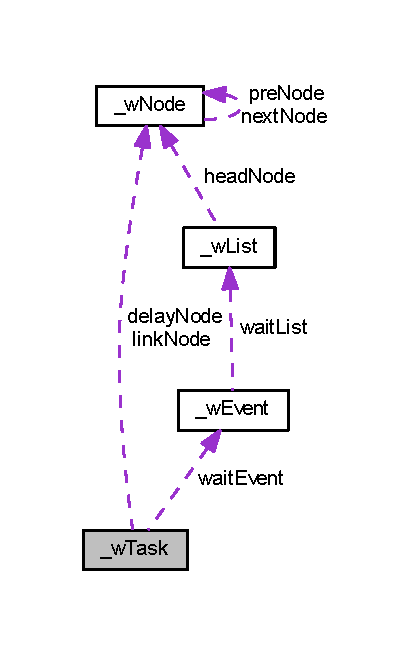
\includegraphics[width=198pt]{struct__w_task__coll__graph}
\end{center}
\end{figure}
\subsection*{成员变量}
\begin{DoxyCompactItemize}
\item 
\mbox{\hyperlink{w_task_8h_ae1dd34929f40dd21d0ea81f2d3f1c2e0}{w\+Task\+Stack}} $\ast$ \mbox{\hyperlink{struct__w_task_aab79976fc944e26844168b6c262e33f8}{stack}}
\item 
uint32\+\_\+t $\ast$ \mbox{\hyperlink{struct__w_task_a57eb489f59ea6a56ccff2efea7f92c33}{stack\+Base}}
\item 
uint32\+\_\+t \mbox{\hyperlink{struct__w_task_ae20ace955faaa4fb797b69b75feef3d3}{stack\+Size}}
\item 
\mbox{\hyperlink{w_lib_8h_a98363f2fc9ff1bef5993786140d900f2}{w\+Node}} \mbox{\hyperlink{struct__w_task_aace0256afebaf717de11433d186f53b2}{link\+Node}}
\item 
uint32\+\_\+t \mbox{\hyperlink{struct__w_task_a0c1ef2b42e60232fd2355246df290c68}{delay\+Ticks}}
\item 
\mbox{\hyperlink{w_lib_8h_a98363f2fc9ff1bef5993786140d900f2}{w\+Node}} \mbox{\hyperlink{struct__w_task_a2dfdbd06053445a3e8869801ea875edc}{delay\+Node}}
\item 
uint32\+\_\+t \mbox{\hyperlink{struct__w_task_a6871573fefee3ad102e26a09e7a2f493}{prio}}
\item 
uint32\+\_\+t \mbox{\hyperlink{struct__w_task_a1b0c7bd4d79798ef4e0ce23894c9aeb2}{state}}
\item 
uint32\+\_\+t \mbox{\hyperlink{struct__w_task_a4fe7f19d35a11368d300b99348451fdd}{slice}}
\item 
uint32\+\_\+t \mbox{\hyperlink{struct__w_task_a70023864793bcef3ab18d4a66832ca6d}{suspend\+Count}}
\item 
void($\ast$ \mbox{\hyperlink{struct__w_task_a9350eb6ea9f174b0711e8835a1543a87}{clean}} )(void $\ast$param)
\item 
void $\ast$ \mbox{\hyperlink{struct__w_task_a44efa3d1143953e06ee78314f155aa92}{cleanparam}}
\item 
uint8\+\_\+t \mbox{\hyperlink{struct__w_task_a3b197900b58be56e296d46207dec079f}{request\+Delete\+Flag}}
\item 
struct \mbox{\hyperlink{struct__w_event}{\+\_\+w\+Event}} $\ast$ \mbox{\hyperlink{struct__w_task_a52896f1a7ded634042291bac3f2b109e}{wait\+Event}}
\item 
void $\ast$ \mbox{\hyperlink{struct__w_task_ae1ae004c581e0cc9fd22662535700001}{event\+Msg}}
\item 
uint32\+\_\+t \mbox{\hyperlink{struct__w_task_a37707d87e42a484588393e5b3683ffbb}{wait\+Event\+Result}}
\item 
uint32\+\_\+t \mbox{\hyperlink{struct__w_task_a35ba8bba537f36efd05f084a5531825a}{wait\+Flags\+Type}}
\item 
uint32\+\_\+t \mbox{\hyperlink{struct__w_task_af713ddc7d68fde45ace722a554f41918}{event\+Flags}}
\end{DoxyCompactItemize}


\subsection{详细描述}
任务结构 

\subsection{结构体成员变量说明}
\mbox{\Hypertarget{struct__w_task_a9350eb6ea9f174b0711e8835a1543a87}\label{struct__w_task_a9350eb6ea9f174b0711e8835a1543a87}} 
\index{\+\_\+w\+Task@{\+\_\+w\+Task}!clean@{clean}}
\index{clean@{clean}!\+\_\+w\+Task@{\+\_\+w\+Task}}
\subsubsection{\texorpdfstring{clean}{clean}}
{\footnotesize\ttfamily void($\ast$ clean) (void $\ast$param)}

任务被删除时调用的清理函数 \mbox{\Hypertarget{struct__w_task_a44efa3d1143953e06ee78314f155aa92}\label{struct__w_task_a44efa3d1143953e06ee78314f155aa92}} 
\index{\+\_\+w\+Task@{\+\_\+w\+Task}!cleanparam@{cleanparam}}
\index{cleanparam@{cleanparam}!\+\_\+w\+Task@{\+\_\+w\+Task}}
\subsubsection{\texorpdfstring{cleanparam}{cleanparam}}
{\footnotesize\ttfamily void$\ast$ cleanparam}

传递给清理函数的参数 \mbox{\Hypertarget{struct__w_task_a2dfdbd06053445a3e8869801ea875edc}\label{struct__w_task_a2dfdbd06053445a3e8869801ea875edc}} 
\index{\+\_\+w\+Task@{\+\_\+w\+Task}!delay\+Node@{delay\+Node}}
\index{delay\+Node@{delay\+Node}!\+\_\+w\+Task@{\+\_\+w\+Task}}
\subsubsection{\texorpdfstring{delay\+Node}{delayNode}}
{\footnotesize\ttfamily \mbox{\hyperlink{w_lib_8h_a98363f2fc9ff1bef5993786140d900f2}{w\+Node}} delay\+Node}

通用延时结点结构 \mbox{\Hypertarget{struct__w_task_a0c1ef2b42e60232fd2355246df290c68}\label{struct__w_task_a0c1ef2b42e60232fd2355246df290c68}} 
\index{\+\_\+w\+Task@{\+\_\+w\+Task}!delay\+Ticks@{delay\+Ticks}}
\index{delay\+Ticks@{delay\+Ticks}!\+\_\+w\+Task@{\+\_\+w\+Task}}
\subsubsection{\texorpdfstring{delay\+Ticks}{delayTicks}}
{\footnotesize\ttfamily uint32\+\_\+t delay\+Ticks}

任务延时个数 \mbox{\Hypertarget{struct__w_task_af713ddc7d68fde45ace722a554f41918}\label{struct__w_task_af713ddc7d68fde45ace722a554f41918}} 
\index{\+\_\+w\+Task@{\+\_\+w\+Task}!event\+Flags@{event\+Flags}}
\index{event\+Flags@{event\+Flags}!\+\_\+w\+Task@{\+\_\+w\+Task}}
\subsubsection{\texorpdfstring{event\+Flags}{eventFlags}}
{\footnotesize\ttfamily uint32\+\_\+t event\+Flags}

等待的事件标志 \mbox{\Hypertarget{struct__w_task_ae1ae004c581e0cc9fd22662535700001}\label{struct__w_task_ae1ae004c581e0cc9fd22662535700001}} 
\index{\+\_\+w\+Task@{\+\_\+w\+Task}!event\+Msg@{event\+Msg}}
\index{event\+Msg@{event\+Msg}!\+\_\+w\+Task@{\+\_\+w\+Task}}
\subsubsection{\texorpdfstring{event\+Msg}{eventMsg}}
{\footnotesize\ttfamily void$\ast$ event\+Msg}

等待事件的数据存放位置 \mbox{\Hypertarget{struct__w_task_aace0256afebaf717de11433d186f53b2}\label{struct__w_task_aace0256afebaf717de11433d186f53b2}} 
\index{\+\_\+w\+Task@{\+\_\+w\+Task}!link\+Node@{link\+Node}}
\index{link\+Node@{link\+Node}!\+\_\+w\+Task@{\+\_\+w\+Task}}
\subsubsection{\texorpdfstring{link\+Node}{linkNode}}
{\footnotesize\ttfamily \mbox{\hyperlink{w_lib_8h_a98363f2fc9ff1bef5993786140d900f2}{w\+Node}} link\+Node}

优先级队列链接结点 \mbox{\Hypertarget{struct__w_task_a6871573fefee3ad102e26a09e7a2f493}\label{struct__w_task_a6871573fefee3ad102e26a09e7a2f493}} 
\index{\+\_\+w\+Task@{\+\_\+w\+Task}!prio@{prio}}
\index{prio@{prio}!\+\_\+w\+Task@{\+\_\+w\+Task}}
\subsubsection{\texorpdfstring{prio}{prio}}
{\footnotesize\ttfamily uint32\+\_\+t prio}

任务优先级 \mbox{\Hypertarget{struct__w_task_a3b197900b58be56e296d46207dec079f}\label{struct__w_task_a3b197900b58be56e296d46207dec079f}} 
\index{\+\_\+w\+Task@{\+\_\+w\+Task}!request\+Delete\+Flag@{request\+Delete\+Flag}}
\index{request\+Delete\+Flag@{request\+Delete\+Flag}!\+\_\+w\+Task@{\+\_\+w\+Task}}
\subsubsection{\texorpdfstring{request\+Delete\+Flag}{requestDeleteFlag}}
{\footnotesize\ttfamily uint8\+\_\+t request\+Delete\+Flag}

请求删除标志 \mbox{\Hypertarget{struct__w_task_a4fe7f19d35a11368d300b99348451fdd}\label{struct__w_task_a4fe7f19d35a11368d300b99348451fdd}} 
\index{\+\_\+w\+Task@{\+\_\+w\+Task}!slice@{slice}}
\index{slice@{slice}!\+\_\+w\+Task@{\+\_\+w\+Task}}
\subsubsection{\texorpdfstring{slice}{slice}}
{\footnotesize\ttfamily uint32\+\_\+t slice}

时间片计数器 \mbox{\Hypertarget{struct__w_task_aab79976fc944e26844168b6c262e33f8}\label{struct__w_task_aab79976fc944e26844168b6c262e33f8}} 
\index{\+\_\+w\+Task@{\+\_\+w\+Task}!stack@{stack}}
\index{stack@{stack}!\+\_\+w\+Task@{\+\_\+w\+Task}}
\subsubsection{\texorpdfstring{stack}{stack}}
{\footnotesize\ttfamily \mbox{\hyperlink{w_task_8h_ae1dd34929f40dd21d0ea81f2d3f1c2e0}{w\+Task\+Stack}}$\ast$ stack}

任务堆栈指针 \mbox{\Hypertarget{struct__w_task_a57eb489f59ea6a56ccff2efea7f92c33}\label{struct__w_task_a57eb489f59ea6a56ccff2efea7f92c33}} 
\index{\+\_\+w\+Task@{\+\_\+w\+Task}!stack\+Base@{stack\+Base}}
\index{stack\+Base@{stack\+Base}!\+\_\+w\+Task@{\+\_\+w\+Task}}
\subsubsection{\texorpdfstring{stack\+Base}{stackBase}}
{\footnotesize\ttfamily uint32\+\_\+t$\ast$ stack\+Base}

任务堆栈首地址 \mbox{\Hypertarget{struct__w_task_ae20ace955faaa4fb797b69b75feef3d3}\label{struct__w_task_ae20ace955faaa4fb797b69b75feef3d3}} 
\index{\+\_\+w\+Task@{\+\_\+w\+Task}!stack\+Size@{stack\+Size}}
\index{stack\+Size@{stack\+Size}!\+\_\+w\+Task@{\+\_\+w\+Task}}
\subsubsection{\texorpdfstring{stack\+Size}{stackSize}}
{\footnotesize\ttfamily uint32\+\_\+t stack\+Size}

堆栈大小 \mbox{\Hypertarget{struct__w_task_a1b0c7bd4d79798ef4e0ce23894c9aeb2}\label{struct__w_task_a1b0c7bd4d79798ef4e0ce23894c9aeb2}} 
\index{\+\_\+w\+Task@{\+\_\+w\+Task}!state@{state}}
\index{state@{state}!\+\_\+w\+Task@{\+\_\+w\+Task}}
\subsubsection{\texorpdfstring{state}{state}}
{\footnotesize\ttfamily uint32\+\_\+t state}

状态字段,用于判断是不是处于延时状态 \mbox{\Hypertarget{struct__w_task_a70023864793bcef3ab18d4a66832ca6d}\label{struct__w_task_a70023864793bcef3ab18d4a66832ca6d}} 
\index{\+\_\+w\+Task@{\+\_\+w\+Task}!suspend\+Count@{suspend\+Count}}
\index{suspend\+Count@{suspend\+Count}!\+\_\+w\+Task@{\+\_\+w\+Task}}
\subsubsection{\texorpdfstring{suspend\+Count}{suspendCount}}
{\footnotesize\ttfamily uint32\+\_\+t suspend\+Count}

挂起状态计数器 \mbox{\Hypertarget{struct__w_task_a52896f1a7ded634042291bac3f2b109e}\label{struct__w_task_a52896f1a7ded634042291bac3f2b109e}} 
\index{\+\_\+w\+Task@{\+\_\+w\+Task}!wait\+Event@{wait\+Event}}
\index{wait\+Event@{wait\+Event}!\+\_\+w\+Task@{\+\_\+w\+Task}}
\subsubsection{\texorpdfstring{wait\+Event}{waitEvent}}
{\footnotesize\ttfamily struct \mbox{\hyperlink{struct__w_event}{\+\_\+w\+Event}}$\ast$ wait\+Event}

正在等待的任务控制块 \mbox{\Hypertarget{struct__w_task_a37707d87e42a484588393e5b3683ffbb}\label{struct__w_task_a37707d87e42a484588393e5b3683ffbb}} 
\index{\+\_\+w\+Task@{\+\_\+w\+Task}!wait\+Event\+Result@{wait\+Event\+Result}}
\index{wait\+Event\+Result@{wait\+Event\+Result}!\+\_\+w\+Task@{\+\_\+w\+Task}}
\subsubsection{\texorpdfstring{wait\+Event\+Result}{waitEventResult}}
{\footnotesize\ttfamily uint32\+\_\+t wait\+Event\+Result}

等待事件的结果 \mbox{\Hypertarget{struct__w_task_a35ba8bba537f36efd05f084a5531825a}\label{struct__w_task_a35ba8bba537f36efd05f084a5531825a}} 
\index{\+\_\+w\+Task@{\+\_\+w\+Task}!wait\+Flags\+Type@{wait\+Flags\+Type}}
\index{wait\+Flags\+Type@{wait\+Flags\+Type}!\+\_\+w\+Task@{\+\_\+w\+Task}}
\subsubsection{\texorpdfstring{wait\+Flags\+Type}{waitFlagsType}}
{\footnotesize\ttfamily uint32\+\_\+t wait\+Flags\+Type}

等待的事件方式 

该结构体的文档由以下文件生成\+:\begin{DoxyCompactItemize}
\item 
C\+:/\+Users/pc/\+Desktop/\+W\+Q\+\_\+\+O\+S/\+Project/\+Sourse/\mbox{\hyperlink{w_task_8h}{w\+Task.\+h}}\end{DoxyCompactItemize}

\hypertarget{struct__w_task_info}{}\section{\+\_\+w\+Task\+Info结构体 参考}
\label{struct__w_task_info}\index{\+\_\+w\+Task\+Info@{\+\_\+w\+Task\+Info}}


任务相关信息结构  




{\ttfamily \#include $<$w\+Task.\+h$>$}

\subsection*{成员变量}
\begin{DoxyCompactItemize}
\item 
uint32\+\_\+t \mbox{\hyperlink{struct__w_task_info_a0c1ef2b42e60232fd2355246df290c68}{delay\+Ticks}}
\item 
uint32\+\_\+t \mbox{\hyperlink{struct__w_task_info_a6871573fefee3ad102e26a09e7a2f493}{prio}}
\item 
uint32\+\_\+t \mbox{\hyperlink{struct__w_task_info_a1b0c7bd4d79798ef4e0ce23894c9aeb2}{state}}
\item 
uint32\+\_\+t \mbox{\hyperlink{struct__w_task_info_a4fe7f19d35a11368d300b99348451fdd}{slice}}
\item 
uint32\+\_\+t \mbox{\hyperlink{struct__w_task_info_a70023864793bcef3ab18d4a66832ca6d}{suspend\+Count}}
\item 
uint32\+\_\+t \mbox{\hyperlink{struct__w_task_info_ae20ace955faaa4fb797b69b75feef3d3}{stack\+Size}}
\item 
uint32\+\_\+t \mbox{\hyperlink{struct__w_task_info_ab8b8202c533d50459f39dfab24e8873d}{stack\+Free}}
\end{DoxyCompactItemize}


\subsection{详细描述}
任务相关信息结构 

\subsection{结构体成员变量说明}
\mbox{\Hypertarget{struct__w_task_info_a0c1ef2b42e60232fd2355246df290c68}\label{struct__w_task_info_a0c1ef2b42e60232fd2355246df290c68}} 
\index{\+\_\+w\+Task\+Info@{\+\_\+w\+Task\+Info}!delay\+Ticks@{delay\+Ticks}}
\index{delay\+Ticks@{delay\+Ticks}!\+\_\+w\+Task\+Info@{\+\_\+w\+Task\+Info}}
\subsubsection{\texorpdfstring{delay\+Ticks}{delayTicks}}
{\footnotesize\ttfamily uint32\+\_\+t delay\+Ticks}

延时计数器 \mbox{\Hypertarget{struct__w_task_info_a6871573fefee3ad102e26a09e7a2f493}\label{struct__w_task_info_a6871573fefee3ad102e26a09e7a2f493}} 
\index{\+\_\+w\+Task\+Info@{\+\_\+w\+Task\+Info}!prio@{prio}}
\index{prio@{prio}!\+\_\+w\+Task\+Info@{\+\_\+w\+Task\+Info}}
\subsubsection{\texorpdfstring{prio}{prio}}
{\footnotesize\ttfamily uint32\+\_\+t prio}

任务优先级 \mbox{\Hypertarget{struct__w_task_info_a4fe7f19d35a11368d300b99348451fdd}\label{struct__w_task_info_a4fe7f19d35a11368d300b99348451fdd}} 
\index{\+\_\+w\+Task\+Info@{\+\_\+w\+Task\+Info}!slice@{slice}}
\index{slice@{slice}!\+\_\+w\+Task\+Info@{\+\_\+w\+Task\+Info}}
\subsubsection{\texorpdfstring{slice}{slice}}
{\footnotesize\ttfamily uint32\+\_\+t slice}

当前剩余的时间片 \mbox{\Hypertarget{struct__w_task_info_ab8b8202c533d50459f39dfab24e8873d}\label{struct__w_task_info_ab8b8202c533d50459f39dfab24e8873d}} 
\index{\+\_\+w\+Task\+Info@{\+\_\+w\+Task\+Info}!stack\+Free@{stack\+Free}}
\index{stack\+Free@{stack\+Free}!\+\_\+w\+Task\+Info@{\+\_\+w\+Task\+Info}}
\subsubsection{\texorpdfstring{stack\+Free}{stackFree}}
{\footnotesize\ttfamily uint32\+\_\+t stack\+Free}

空闲堆栈大小 \mbox{\Hypertarget{struct__w_task_info_ae20ace955faaa4fb797b69b75feef3d3}\label{struct__w_task_info_ae20ace955faaa4fb797b69b75feef3d3}} 
\index{\+\_\+w\+Task\+Info@{\+\_\+w\+Task\+Info}!stack\+Size@{stack\+Size}}
\index{stack\+Size@{stack\+Size}!\+\_\+w\+Task\+Info@{\+\_\+w\+Task\+Info}}
\subsubsection{\texorpdfstring{stack\+Size}{stackSize}}
{\footnotesize\ttfamily uint32\+\_\+t stack\+Size}

堆栈大小 \mbox{\Hypertarget{struct__w_task_info_a1b0c7bd4d79798ef4e0ce23894c9aeb2}\label{struct__w_task_info_a1b0c7bd4d79798ef4e0ce23894c9aeb2}} 
\index{\+\_\+w\+Task\+Info@{\+\_\+w\+Task\+Info}!state@{state}}
\index{state@{state}!\+\_\+w\+Task\+Info@{\+\_\+w\+Task\+Info}}
\subsubsection{\texorpdfstring{state}{state}}
{\footnotesize\ttfamily uint32\+\_\+t state}

任务当前状态 \mbox{\Hypertarget{struct__w_task_info_a70023864793bcef3ab18d4a66832ca6d}\label{struct__w_task_info_a70023864793bcef3ab18d4a66832ca6d}} 
\index{\+\_\+w\+Task\+Info@{\+\_\+w\+Task\+Info}!suspend\+Count@{suspend\+Count}}
\index{suspend\+Count@{suspend\+Count}!\+\_\+w\+Task\+Info@{\+\_\+w\+Task\+Info}}
\subsubsection{\texorpdfstring{suspend\+Count}{suspendCount}}
{\footnotesize\ttfamily uint32\+\_\+t suspend\+Count}

被挂起的次数 

该结构体的文档由以下文件生成\+:\begin{DoxyCompactItemize}
\item 
C\+:/\+Users/pc/\+Desktop/\+W\+Q\+\_\+\+O\+S/\+Project/\+Sourse/\mbox{\hyperlink{w_task_8h}{w\+Task.\+h}}\end{DoxyCompactItemize}

\hypertarget{struct__w_timer}{}\section{\+\_\+w\+Timer结构体 参考}
\label{struct__w_timer}\index{\+\_\+w\+Timer@{\+\_\+w\+Timer}}


定义软件定时器类型  




{\ttfamily \#include $<$w\+Timer.\+h$>$}



\+\_\+w\+Timer 的协作图\+:
\nopagebreak
\begin{figure}[H]
\begin{center}
\leavevmode
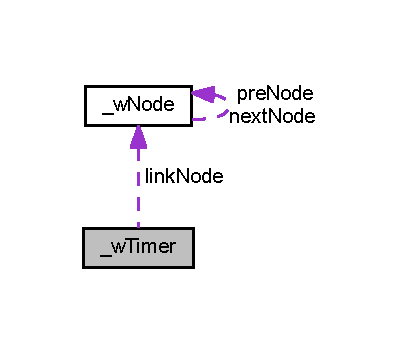
\includegraphics[width=192pt]{struct__w_timer__coll__graph}
\end{center}
\end{figure}
\subsection*{成员变量}
\begin{DoxyCompactItemize}
\item 
\mbox{\hyperlink{w_lib_8h_a98363f2fc9ff1bef5993786140d900f2}{w\+Node}} \mbox{\hyperlink{struct__w_timer_aace0256afebaf717de11433d186f53b2}{link\+Node}}
\item 
uint32\+\_\+t \mbox{\hyperlink{struct__w_timer_acecf013811265c398517a464e7e6f7b2}{start\+Delay\+Ticks}}
\item 
uint32\+\_\+t \mbox{\hyperlink{struct__w_timer_a95f8cbd7a4ba89fc9ae542eb04a24bc0}{duration\+Ticks}}
\item 
uint32\+\_\+t \mbox{\hyperlink{struct__w_timer_a0c1ef2b42e60232fd2355246df290c68}{delay\+Ticks}}
\item 
void($\ast$ \mbox{\hyperlink{struct__w_timer_a5b39f4308b8e715d9278cbf70f7297c7}{timer\+Func}} )(void $\ast$\mbox{\hyperlink{struct__w_timer_a9ce2ec4812a92cb6ab39f6e81e9173a9}{arg}})
\item 
void $\ast$ \mbox{\hyperlink{struct__w_timer_a9ce2ec4812a92cb6ab39f6e81e9173a9}{arg}}
\item 
uint32\+\_\+t \mbox{\hyperlink{struct__w_timer_ac0c635110dc503f164fff91b163936d7}{config}}
\item 
\mbox{\hyperlink{w_timer_8h_afd5ce485f9f6080eb16b9b0d11c09dcd}{w\+Timer\+State}} \mbox{\hyperlink{struct__w_timer_ac82a56d0e6704cdcfdad6e80803b1674}{state}}
\end{DoxyCompactItemize}


\subsection{详细描述}
定义软件定时器类型 

\subsection{结构体成员变量说明}
\mbox{\Hypertarget{struct__w_timer_a9ce2ec4812a92cb6ab39f6e81e9173a9}\label{struct__w_timer_a9ce2ec4812a92cb6ab39f6e81e9173a9}} 
\index{\+\_\+w\+Timer@{\+\_\+w\+Timer}!arg@{arg}}
\index{arg@{arg}!\+\_\+w\+Timer@{\+\_\+w\+Timer}}
\subsubsection{\texorpdfstring{arg}{arg}}
{\footnotesize\ttfamily void$\ast$ arg}

传给回调函数的参数 \mbox{\Hypertarget{struct__w_timer_ac0c635110dc503f164fff91b163936d7}\label{struct__w_timer_ac0c635110dc503f164fff91b163936d7}} 
\index{\+\_\+w\+Timer@{\+\_\+w\+Timer}!config@{config}}
\index{config@{config}!\+\_\+w\+Timer@{\+\_\+w\+Timer}}
\subsubsection{\texorpdfstring{config}{config}}
{\footnotesize\ttfamily uint32\+\_\+t config}

定时器配置参数 \mbox{\Hypertarget{struct__w_timer_a0c1ef2b42e60232fd2355246df290c68}\label{struct__w_timer_a0c1ef2b42e60232fd2355246df290c68}} 
\index{\+\_\+w\+Timer@{\+\_\+w\+Timer}!delay\+Ticks@{delay\+Ticks}}
\index{delay\+Ticks@{delay\+Ticks}!\+\_\+w\+Timer@{\+\_\+w\+Timer}}
\subsubsection{\texorpdfstring{delay\+Ticks}{delayTicks}}
{\footnotesize\ttfamily uint32\+\_\+t delay\+Ticks}

当前定时递减计数值 \mbox{\Hypertarget{struct__w_timer_a95f8cbd7a4ba89fc9ae542eb04a24bc0}\label{struct__w_timer_a95f8cbd7a4ba89fc9ae542eb04a24bc0}} 
\index{\+\_\+w\+Timer@{\+\_\+w\+Timer}!duration\+Ticks@{duration\+Ticks}}
\index{duration\+Ticks@{duration\+Ticks}!\+\_\+w\+Timer@{\+\_\+w\+Timer}}
\subsubsection{\texorpdfstring{duration\+Ticks}{durationTicks}}
{\footnotesize\ttfamily uint32\+\_\+t duration\+Ticks}

周期定时时的ticks数 \mbox{\Hypertarget{struct__w_timer_aace0256afebaf717de11433d186f53b2}\label{struct__w_timer_aace0256afebaf717de11433d186f53b2}} 
\index{\+\_\+w\+Timer@{\+\_\+w\+Timer}!link\+Node@{link\+Node}}
\index{link\+Node@{link\+Node}!\+\_\+w\+Timer@{\+\_\+w\+Timer}}
\subsubsection{\texorpdfstring{link\+Node}{linkNode}}
{\footnotesize\ttfamily \mbox{\hyperlink{w_lib_8h_a98363f2fc9ff1bef5993786140d900f2}{w\+Node}} link\+Node}

链表结点 \mbox{\Hypertarget{struct__w_timer_acecf013811265c398517a464e7e6f7b2}\label{struct__w_timer_acecf013811265c398517a464e7e6f7b2}} 
\index{\+\_\+w\+Timer@{\+\_\+w\+Timer}!start\+Delay\+Ticks@{start\+Delay\+Ticks}}
\index{start\+Delay\+Ticks@{start\+Delay\+Ticks}!\+\_\+w\+Timer@{\+\_\+w\+Timer}}
\subsubsection{\texorpdfstring{start\+Delay\+Ticks}{startDelayTicks}}
{\footnotesize\ttfamily uint32\+\_\+t start\+Delay\+Ticks}

初次启动后的ticks数 \mbox{\Hypertarget{struct__w_timer_ac82a56d0e6704cdcfdad6e80803b1674}\label{struct__w_timer_ac82a56d0e6704cdcfdad6e80803b1674}} 
\index{\+\_\+w\+Timer@{\+\_\+w\+Timer}!state@{state}}
\index{state@{state}!\+\_\+w\+Timer@{\+\_\+w\+Timer}}
\subsubsection{\texorpdfstring{state}{state}}
{\footnotesize\ttfamily \mbox{\hyperlink{w_timer_8h_afd5ce485f9f6080eb16b9b0d11c09dcd}{w\+Timer\+State}} state}

定时器状态 \mbox{\Hypertarget{struct__w_timer_a5b39f4308b8e715d9278cbf70f7297c7}\label{struct__w_timer_a5b39f4308b8e715d9278cbf70f7297c7}} 
\index{\+\_\+w\+Timer@{\+\_\+w\+Timer}!timer\+Func@{timer\+Func}}
\index{timer\+Func@{timer\+Func}!\+\_\+w\+Timer@{\+\_\+w\+Timer}}
\subsubsection{\texorpdfstring{timer\+Func}{timerFunc}}
{\footnotesize\ttfamily void($\ast$ timer\+Func) (void $\ast$\mbox{\hyperlink{struct__w_timer_a9ce2ec4812a92cb6ab39f6e81e9173a9}{arg}})}

定时回调函数 

该结构体的文档由以下文件生成\+:\begin{DoxyCompactItemize}
\item 
C\+:/\+Users/pc/\+Desktop/\+W\+Q\+\_\+\+O\+S/\+Project/\+Sourse/\mbox{\hyperlink{w_timer_8h}{w\+Timer.\+h}}\end{DoxyCompactItemize}

\hypertarget{struct__w_timer_info}{}\section{\+\_\+w\+Timer\+Info结构体 参考}
\label{struct__w_timer_info}\index{\+\_\+w\+Timer\+Info@{\+\_\+w\+Timer\+Info}}


定义软件定时器信息结构  




{\ttfamily \#include $<$w\+Timer.\+h$>$}

\subsection*{成员变量}
\begin{DoxyCompactItemize}
\item 
uint32\+\_\+t \mbox{\hyperlink{struct__w_timer_info_acecf013811265c398517a464e7e6f7b2}{start\+Delay\+Ticks}}
\item 
uint32\+\_\+t \mbox{\hyperlink{struct__w_timer_info_a95f8cbd7a4ba89fc9ae542eb04a24bc0}{duration\+Ticks}}
\item 
void($\ast$ \mbox{\hyperlink{struct__w_timer_info_a5b39f4308b8e715d9278cbf70f7297c7}{timer\+Func}} )(void $\ast$\mbox{\hyperlink{struct__w_timer_info_a9ce2ec4812a92cb6ab39f6e81e9173a9}{arg}})
\item 
void $\ast$ \mbox{\hyperlink{struct__w_timer_info_a9ce2ec4812a92cb6ab39f6e81e9173a9}{arg}}
\item 
uint32\+\_\+t \mbox{\hyperlink{struct__w_timer_info_ac0c635110dc503f164fff91b163936d7}{config}}
\item 
\mbox{\hyperlink{w_timer_8h_afd5ce485f9f6080eb16b9b0d11c09dcd}{w\+Timer\+State}} \mbox{\hyperlink{struct__w_timer_info_ac82a56d0e6704cdcfdad6e80803b1674}{state}}
\end{DoxyCompactItemize}


\subsection{详细描述}
定义软件定时器信息结构 

\subsection{结构体成员变量说明}
\mbox{\Hypertarget{struct__w_timer_info_a9ce2ec4812a92cb6ab39f6e81e9173a9}\label{struct__w_timer_info_a9ce2ec4812a92cb6ab39f6e81e9173a9}} 
\index{\+\_\+w\+Timer\+Info@{\+\_\+w\+Timer\+Info}!arg@{arg}}
\index{arg@{arg}!\+\_\+w\+Timer\+Info@{\+\_\+w\+Timer\+Info}}
\subsubsection{\texorpdfstring{arg}{arg}}
{\footnotesize\ttfamily void$\ast$ arg}

传递给回调函数的参数 \mbox{\Hypertarget{struct__w_timer_info_ac0c635110dc503f164fff91b163936d7}\label{struct__w_timer_info_ac0c635110dc503f164fff91b163936d7}} 
\index{\+\_\+w\+Timer\+Info@{\+\_\+w\+Timer\+Info}!config@{config}}
\index{config@{config}!\+\_\+w\+Timer\+Info@{\+\_\+w\+Timer\+Info}}
\subsubsection{\texorpdfstring{config}{config}}
{\footnotesize\ttfamily uint32\+\_\+t config}

定时器配置参数 \mbox{\Hypertarget{struct__w_timer_info_a95f8cbd7a4ba89fc9ae542eb04a24bc0}\label{struct__w_timer_info_a95f8cbd7a4ba89fc9ae542eb04a24bc0}} 
\index{\+\_\+w\+Timer\+Info@{\+\_\+w\+Timer\+Info}!duration\+Ticks@{duration\+Ticks}}
\index{duration\+Ticks@{duration\+Ticks}!\+\_\+w\+Timer\+Info@{\+\_\+w\+Timer\+Info}}
\subsubsection{\texorpdfstring{duration\+Ticks}{durationTicks}}
{\footnotesize\ttfamily uint32\+\_\+t duration\+Ticks}

周期定时时的周期tick数 \mbox{\Hypertarget{struct__w_timer_info_acecf013811265c398517a464e7e6f7b2}\label{struct__w_timer_info_acecf013811265c398517a464e7e6f7b2}} 
\index{\+\_\+w\+Timer\+Info@{\+\_\+w\+Timer\+Info}!start\+Delay\+Ticks@{start\+Delay\+Ticks}}
\index{start\+Delay\+Ticks@{start\+Delay\+Ticks}!\+\_\+w\+Timer\+Info@{\+\_\+w\+Timer\+Info}}
\subsubsection{\texorpdfstring{start\+Delay\+Ticks}{startDelayTicks}}
{\footnotesize\ttfamily uint32\+\_\+t start\+Delay\+Ticks}

初次启动延后的ticks数 \mbox{\Hypertarget{struct__w_timer_info_ac82a56d0e6704cdcfdad6e80803b1674}\label{struct__w_timer_info_ac82a56d0e6704cdcfdad6e80803b1674}} 
\index{\+\_\+w\+Timer\+Info@{\+\_\+w\+Timer\+Info}!state@{state}}
\index{state@{state}!\+\_\+w\+Timer\+Info@{\+\_\+w\+Timer\+Info}}
\subsubsection{\texorpdfstring{state}{state}}
{\footnotesize\ttfamily \mbox{\hyperlink{w_timer_8h_afd5ce485f9f6080eb16b9b0d11c09dcd}{w\+Timer\+State}} state}

定时器状态 \mbox{\Hypertarget{struct__w_timer_info_a5b39f4308b8e715d9278cbf70f7297c7}\label{struct__w_timer_info_a5b39f4308b8e715d9278cbf70f7297c7}} 
\index{\+\_\+w\+Timer\+Info@{\+\_\+w\+Timer\+Info}!timer\+Func@{timer\+Func}}
\index{timer\+Func@{timer\+Func}!\+\_\+w\+Timer\+Info@{\+\_\+w\+Timer\+Info}}
\subsubsection{\texorpdfstring{timer\+Func}{timerFunc}}
{\footnotesize\ttfamily void($\ast$ timer\+Func) (void $\ast$\mbox{\hyperlink{struct__w_timer_info_a9ce2ec4812a92cb6ab39f6e81e9173a9}{arg}})}

定时回调函数 

该结构体的文档由以下文件生成\+:\begin{DoxyCompactItemize}
\item 
C\+:/\+Users/pc/\+Desktop/\+W\+Q\+\_\+\+O\+S/\+Project/\+Sourse/\mbox{\hyperlink{w_timer_8h}{w\+Timer.\+h}}\end{DoxyCompactItemize}

\hypertarget{structw_bitmap}{}\section{w\+Bitmap结构体 参考}
\label{structw_bitmap}\index{w\+Bitmap@{w\+Bitmap}}


{\ttfamily \#include $<$w\+Lib.\+h$>$}

\subsection*{成员变量}
\begin{DoxyCompactItemize}
\item 
uint32\+\_\+t \mbox{\hyperlink{structw_bitmap_adc5b4308ed7b0d1a073896de1d25636a}{bitmap}}
\end{DoxyCompactItemize}


\subsection{结构体成员变量说明}
\mbox{\Hypertarget{structw_bitmap_adc5b4308ed7b0d1a073896de1d25636a}\label{structw_bitmap_adc5b4308ed7b0d1a073896de1d25636a}} 
\index{w\+Bitmap@{w\+Bitmap}!bitmap@{bitmap}}
\index{bitmap@{bitmap}!w\+Bitmap@{w\+Bitmap}}
\subsubsection{\texorpdfstring{bitmap}{bitmap}}
{\footnotesize\ttfamily uint32\+\_\+t bitmap}



该结构体的文档由以下文件生成\+:\begin{DoxyCompactItemize}
\item 
C\+:/\+Users/pc/\+Desktop/\+W\+Q\+\_\+\+O\+S/\+Project/\+Sourse/\mbox{\hyperlink{w_lib_8h}{w\+Lib.\+h}}\end{DoxyCompactItemize}

\chapter{文件说明}
\hypertarget{_r_t_e___components_8h}{}\section{C\+:/\+Users/pc/\+Desktop/\+W\+Q\+\_\+\+O\+S/\+Project/\+R\+T\+E/\+\_\+\+Target\+\_\+1/\+R\+T\+E\+\_\+\+Components.h 文件参考}
\label{_r_t_e___components_8h}\index{C\+:/\+Users/pc/\+Desktop/\+W\+Q\+\_\+\+O\+S/\+Project/\+R\+T\+E/\+\_\+\+Target\+\_\+1/\+R\+T\+E\+\_\+\+Components.\+h@{C\+:/\+Users/pc/\+Desktop/\+W\+Q\+\_\+\+O\+S/\+Project/\+R\+T\+E/\+\_\+\+Target\+\_\+1/\+R\+T\+E\+\_\+\+Components.\+h}}
\subsection*{宏定义}
\begin{DoxyCompactItemize}
\item 
\#define \mbox{\hyperlink{_r_t_e___components_8h_ad6db6908b5ef4d6a4f5423a39f1a4392}{C\+M\+S\+I\+S\+\_\+device\+\_\+header}}~\char`\"{}A\+R\+M\+C\+M3.\+h\char`\"{}
\end{DoxyCompactItemize}


\subsection{宏定义说明}
\mbox{\Hypertarget{_r_t_e___components_8h_ad6db6908b5ef4d6a4f5423a39f1a4392}\label{_r_t_e___components_8h_ad6db6908b5ef4d6a4f5423a39f1a4392}} 
\index{R\+T\+E\+\_\+\+Components.\+h@{R\+T\+E\+\_\+\+Components.\+h}!C\+M\+S\+I\+S\+\_\+device\+\_\+header@{C\+M\+S\+I\+S\+\_\+device\+\_\+header}}
\index{C\+M\+S\+I\+S\+\_\+device\+\_\+header@{C\+M\+S\+I\+S\+\_\+device\+\_\+header}!R\+T\+E\+\_\+\+Components.\+h@{R\+T\+E\+\_\+\+Components.\+h}}
\subsubsection{\texorpdfstring{C\+M\+S\+I\+S\+\_\+device\+\_\+header}{CMSIS\_device\_header}}
{\footnotesize\ttfamily \#define C\+M\+S\+I\+S\+\_\+device\+\_\+header~\char`\"{}A\+R\+M\+C\+M3.\+h\char`\"{}}


\hypertarget{system___a_r_m_c_m3_8c}{}\section{C\+:/\+Users/pc/\+Desktop/\+W\+Q\+\_\+\+O\+S/\+Project/\+R\+T\+E/\+Device/\+A\+R\+M\+C\+M3/system\+\_\+\+A\+R\+M\+C\+M3.c 文件参考}
\label{system___a_r_m_c_m3_8c}\index{C\+:/\+Users/pc/\+Desktop/\+W\+Q\+\_\+\+O\+S/\+Project/\+R\+T\+E/\+Device/\+A\+R\+M\+C\+M3/system\+\_\+\+A\+R\+M\+C\+M3.\+c@{C\+:/\+Users/pc/\+Desktop/\+W\+Q\+\_\+\+O\+S/\+Project/\+R\+T\+E/\+Device/\+A\+R\+M\+C\+M3/system\+\_\+\+A\+R\+M\+C\+M3.\+c}}


C\+M\+S\+IS Device System Source File for A\+R\+M\+C\+M3 Device Series  


{\ttfamily \#include \char`\"{}A\+R\+M\+C\+M3.\+h\char`\"{}}\newline
system\+\_\+\+A\+R\+M\+C\+M3.\+c 的引用(Include)关系图\+:
\nopagebreak
\begin{figure}[H]
\begin{center}
\leavevmode
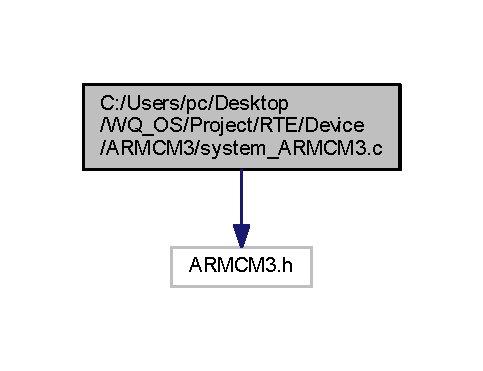
\includegraphics[width=232pt]{system___a_r_m_c_m3_8c__incl}
\end{center}
\end{figure}
\subsection*{宏定义}
\begin{DoxyCompactItemize}
\item 
\#define \mbox{\hyperlink{system___a_r_m_c_m3_8c_a3cad0f9b3c40159bd2fbd7f5e60f2fff}{X\+T\+AL}}~( 12000000\+U )      /$\ast$ Oscillator frequency $\ast$/
\item 
\#define \mbox{\hyperlink{system___a_r_m_c_m3_8c_a95982eccb57c2ae35f8ba3d8f0b05653}{S\+Y\+S\+T\+E\+M\+\_\+\+C\+L\+O\+CK}}~(1 $\ast$ \mbox{\hyperlink{system___a_r_m_c_m3_8c_a3cad0f9b3c40159bd2fbd7f5e60f2fff}{X\+T\+AL}})
\end{DoxyCompactItemize}
\subsection*{函数}
\begin{DoxyCompactItemize}
\item 
void \mbox{\hyperlink{system___a_r_m_c_m3_8c_ae0c36a9591fe6e9c45ecb21a794f0f0f}{System\+Core\+Clock\+Update}} (void)
\item 
void \mbox{\hyperlink{system___a_r_m_c_m3_8c_a93f514700ccf00d08dbdcff7f1224eb2}{System\+Init}} (void)
\end{DoxyCompactItemize}
\subsection*{变量}
\begin{DoxyCompactItemize}
\item 
uint32\+\_\+t \mbox{\hyperlink{system___a_r_m_c_m3_8c_aa3cd3e43291e81e795d642b79b6088e6}{System\+Core\+Clock}} = \mbox{\hyperlink{system___a_r_m_c_m3_8c_a95982eccb57c2ae35f8ba3d8f0b05653}{S\+Y\+S\+T\+E\+M\+\_\+\+C\+L\+O\+CK}}
\end{DoxyCompactItemize}


\subsection{详细描述}
C\+M\+S\+IS Device System Source File for A\+R\+M\+C\+M3 Device Series 

\begin{DoxyVersion}{版本}
V5.\+00 
\end{DoxyVersion}
\begin{DoxyDate}{日期}
07. September 2016 
\end{DoxyDate}


\subsection{宏定义说明}
\mbox{\Hypertarget{system___a_r_m_c_m3_8c_a95982eccb57c2ae35f8ba3d8f0b05653}\label{system___a_r_m_c_m3_8c_a95982eccb57c2ae35f8ba3d8f0b05653}} 
\index{system\+\_\+\+A\+R\+M\+C\+M3.\+c@{system\+\_\+\+A\+R\+M\+C\+M3.\+c}!S\+Y\+S\+T\+E\+M\+\_\+\+C\+L\+O\+CK@{S\+Y\+S\+T\+E\+M\+\_\+\+C\+L\+O\+CK}}
\index{S\+Y\+S\+T\+E\+M\+\_\+\+C\+L\+O\+CK@{S\+Y\+S\+T\+E\+M\+\_\+\+C\+L\+O\+CK}!system\+\_\+\+A\+R\+M\+C\+M3.\+c@{system\+\_\+\+A\+R\+M\+C\+M3.\+c}}
\subsubsection{\texorpdfstring{S\+Y\+S\+T\+E\+M\+\_\+\+C\+L\+O\+CK}{SYSTEM\_CLOCK}}
{\footnotesize\ttfamily \#define S\+Y\+S\+T\+E\+M\+\_\+\+C\+L\+O\+CK~(1 $\ast$ \mbox{\hyperlink{system___a_r_m_c_m3_8c_a3cad0f9b3c40159bd2fbd7f5e60f2fff}{X\+T\+AL}})}

\mbox{\Hypertarget{system___a_r_m_c_m3_8c_a3cad0f9b3c40159bd2fbd7f5e60f2fff}\label{system___a_r_m_c_m3_8c_a3cad0f9b3c40159bd2fbd7f5e60f2fff}} 
\index{system\+\_\+\+A\+R\+M\+C\+M3.\+c@{system\+\_\+\+A\+R\+M\+C\+M3.\+c}!X\+T\+AL@{X\+T\+AL}}
\index{X\+T\+AL@{X\+T\+AL}!system\+\_\+\+A\+R\+M\+C\+M3.\+c@{system\+\_\+\+A\+R\+M\+C\+M3.\+c}}
\subsubsection{\texorpdfstring{X\+T\+AL}{XTAL}}
{\footnotesize\ttfamily \#define X\+T\+AL~( 12000000\+U )      /$\ast$ Oscillator frequency $\ast$/}



\subsection{函数说明}
\mbox{\Hypertarget{system___a_r_m_c_m3_8c_ae0c36a9591fe6e9c45ecb21a794f0f0f}\label{system___a_r_m_c_m3_8c_ae0c36a9591fe6e9c45ecb21a794f0f0f}} 
\index{system\+\_\+\+A\+R\+M\+C\+M3.\+c@{system\+\_\+\+A\+R\+M\+C\+M3.\+c}!System\+Core\+Clock\+Update@{System\+Core\+Clock\+Update}}
\index{System\+Core\+Clock\+Update@{System\+Core\+Clock\+Update}!system\+\_\+\+A\+R\+M\+C\+M3.\+c@{system\+\_\+\+A\+R\+M\+C\+M3.\+c}}
\subsubsection{\texorpdfstring{System\+Core\+Clock\+Update()}{SystemCoreClockUpdate()}}
{\footnotesize\ttfamily void System\+Core\+Clock\+Update (\begin{DoxyParamCaption}\item[{void}]{ }\end{DoxyParamCaption})}

\mbox{\Hypertarget{system___a_r_m_c_m3_8c_a93f514700ccf00d08dbdcff7f1224eb2}\label{system___a_r_m_c_m3_8c_a93f514700ccf00d08dbdcff7f1224eb2}} 
\index{system\+\_\+\+A\+R\+M\+C\+M3.\+c@{system\+\_\+\+A\+R\+M\+C\+M3.\+c}!System\+Init@{System\+Init}}
\index{System\+Init@{System\+Init}!system\+\_\+\+A\+R\+M\+C\+M3.\+c@{system\+\_\+\+A\+R\+M\+C\+M3.\+c}}
\subsubsection{\texorpdfstring{System\+Init()}{SystemInit()}}
{\footnotesize\ttfamily void System\+Init (\begin{DoxyParamCaption}\item[{void}]{ }\end{DoxyParamCaption})}



\subsection{变量说明}
\mbox{\Hypertarget{system___a_r_m_c_m3_8c_aa3cd3e43291e81e795d642b79b6088e6}\label{system___a_r_m_c_m3_8c_aa3cd3e43291e81e795d642b79b6088e6}} 
\index{system\+\_\+\+A\+R\+M\+C\+M3.\+c@{system\+\_\+\+A\+R\+M\+C\+M3.\+c}!System\+Core\+Clock@{System\+Core\+Clock}}
\index{System\+Core\+Clock@{System\+Core\+Clock}!system\+\_\+\+A\+R\+M\+C\+M3.\+c@{system\+\_\+\+A\+R\+M\+C\+M3.\+c}}
\subsubsection{\texorpdfstring{System\+Core\+Clock}{SystemCoreClock}}
{\footnotesize\ttfamily uint32\+\_\+t System\+Core\+Clock = \mbox{\hyperlink{system___a_r_m_c_m3_8c_a95982eccb57c2ae35f8ba3d8f0b05653}{S\+Y\+S\+T\+E\+M\+\_\+\+C\+L\+O\+CK}}}


\hypertarget{app_8c}{}\section{C\+:/\+Users/pc/\+Desktop/\+W\+Q\+\_\+\+O\+S/\+Project/\+Sourse/app.c 文件参考}
\label{app_8c}\index{C\+:/\+Users/pc/\+Desktop/\+W\+Q\+\_\+\+O\+S/\+Project/\+Sourse/app.\+c@{C\+:/\+Users/pc/\+Desktop/\+W\+Q\+\_\+\+O\+S/\+Project/\+Sourse/app.\+c}}
{\ttfamily \#include \char`\"{}W\+Q\+\_\+\+O\+S.\+h\char`\"{}}\newline
app.\+c 的引用(Include)关系图\+:
\nopagebreak
\begin{figure}[H]
\begin{center}
\leavevmode
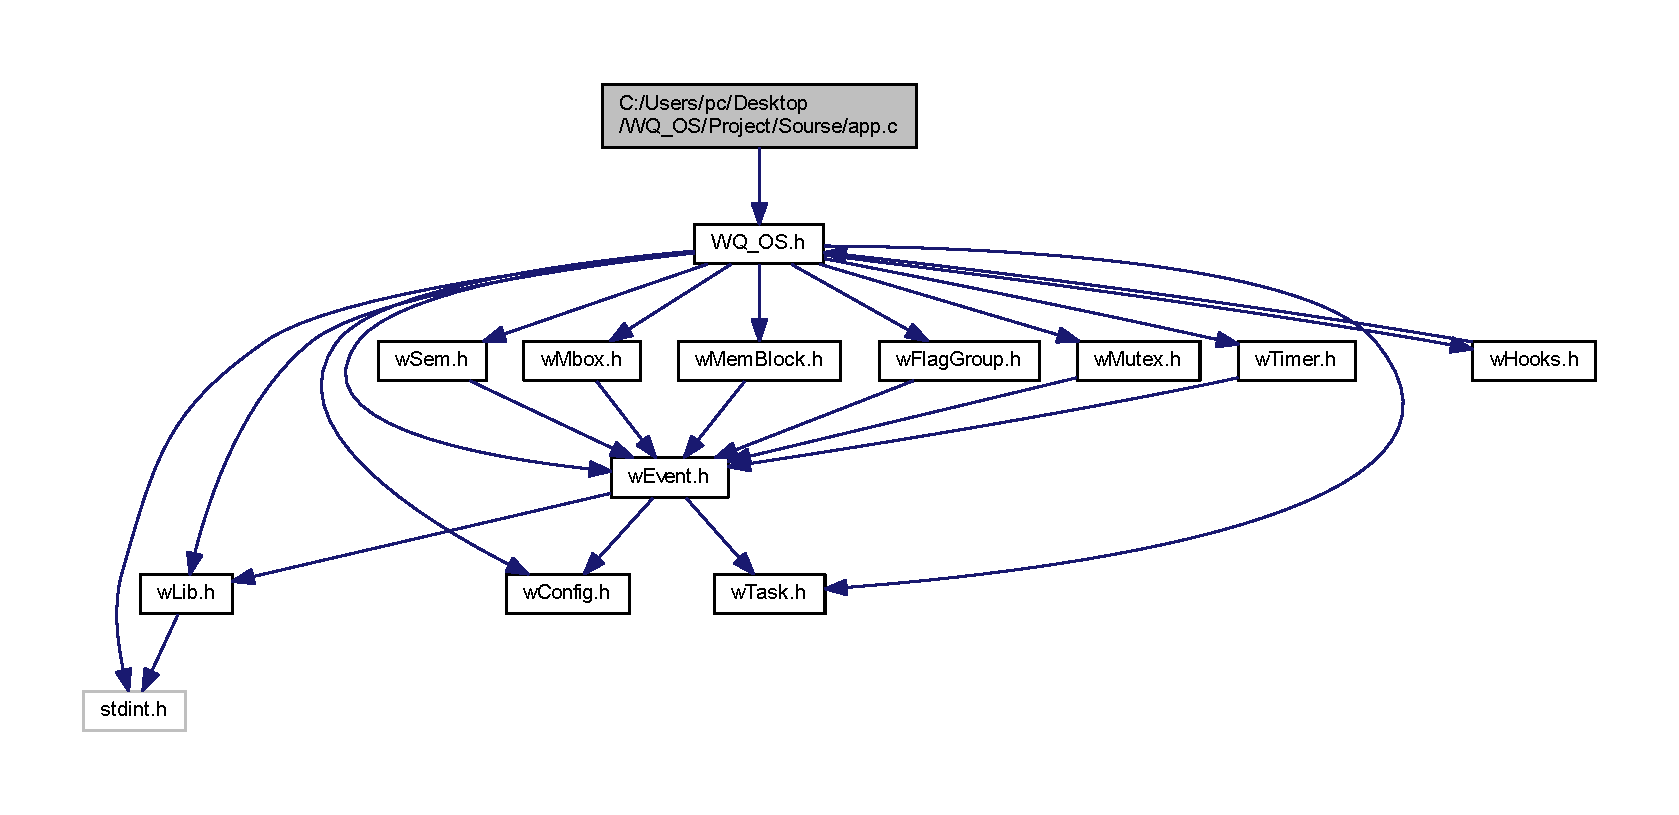
\includegraphics[width=350pt]{app_8c__incl}
\end{center}
\end{figure}
\subsection*{函数}
\begin{DoxyCompactItemize}
\item 
void \mbox{\hyperlink{app_8c_a8eacdcdfdfb9ba0c6a62ee6206d0b1d4}{delay}} (int count)
\begin{DoxyCompactList}\small\item\em 粗暴延时函数 \end{DoxyCompactList}\item 
void \mbox{\hyperlink{app_8c_af8df096cffaabcd535dc2cdfb39a495f}{task1\+Entry}} (void $\ast$param)
\begin{DoxyCompactList}\small\item\em 任务1入口函数 \end{DoxyCompactList}\item 
void \mbox{\hyperlink{app_8c_a58232f2ac8acb8a9d60349af0fd7e8e2}{task2\+Entry}} (void $\ast$param)
\begin{DoxyCompactList}\small\item\em 任务2入口函数 \end{DoxyCompactList}\item 
void \mbox{\hyperlink{app_8c_a771d21a21f591f1b9cdc8b2f834c4a7b}{task3\+Entry}} (void $\ast$param)
\begin{DoxyCompactList}\small\item\em 任务3入口函数 \end{DoxyCompactList}\item 
void \mbox{\hyperlink{app_8c_afe228a3d2729e128c20c88e66a0de25a}{task4\+Entry}} (void $\ast$param)
\begin{DoxyCompactList}\small\item\em 任务4入口函数 \end{DoxyCompactList}\item 
void \mbox{\hyperlink{app_8c_a01fa04097be631417a34fc2b5de3441a}{w\+Init\+App}} (void)
\begin{DoxyCompactList}\small\item\em 任务初始化函数 \end{DoxyCompactList}\end{DoxyCompactItemize}
\subsection*{变量}
\begin{DoxyCompactItemize}
\item 
int \mbox{\hyperlink{app_8c_ad9cda71fc70dc1a2c00cc6e2c34df5af}{task1\+Flag}}
\item 
int \mbox{\hyperlink{app_8c_aee561f6d9d7701291dc07ed736264942}{task2\+Flag}}
\item 
int \mbox{\hyperlink{app_8c_a421a992fc3f38902de45cf746516b7f6}{task3\+Flag}}
\item 
int \mbox{\hyperlink{app_8c_afd6a73505313e637d637b9887894b2a8}{task4\+Flag}}
\item 
\mbox{\hyperlink{w_task_8h_acd0e6238476f631a6ac4588629bac372}{w\+Task}} \mbox{\hyperlink{app_8c_a4712a28475b04585701eb7f2a0050581}{w\+Task1}}
\item 
\mbox{\hyperlink{w_task_8h_acd0e6238476f631a6ac4588629bac372}{w\+Task}} \mbox{\hyperlink{app_8c_ab9f2aab5dabeeef56286973a4195feb4}{w\+Task2}}
\item 
\mbox{\hyperlink{w_task_8h_acd0e6238476f631a6ac4588629bac372}{w\+Task}} \mbox{\hyperlink{app_8c_ab9dc37c449a10dd700b08f218f7ec2d3}{w\+Task3}}
\item 
\mbox{\hyperlink{w_task_8h_acd0e6238476f631a6ac4588629bac372}{w\+Task}} \mbox{\hyperlink{app_8c_a942791273dec5ba24f2c36a6db1c8955}{w\+Task4}}
\item 
\mbox{\hyperlink{w_task_8h_ae1dd34929f40dd21d0ea81f2d3f1c2e0}{w\+Task\+Stack}} \mbox{\hyperlink{app_8c_a5748ce11fa93ad0bd2caf38e20d9f46a}{Task1\+Env}} \mbox{[}1024\mbox{]}
\item 
\mbox{\hyperlink{w_task_8h_ae1dd34929f40dd21d0ea81f2d3f1c2e0}{w\+Task\+Stack}} \mbox{\hyperlink{app_8c_a3228f67bea2c914f9e32333ed07a165f}{Task2\+Env}} \mbox{[}1024\mbox{]}
\item 
\mbox{\hyperlink{w_task_8h_ae1dd34929f40dd21d0ea81f2d3f1c2e0}{w\+Task\+Stack}} \mbox{\hyperlink{app_8c_a71e290c848fe4fe968c811cc1ef1c46b}{Task3\+Env}} \mbox{[}1024\mbox{]}
\item 
\mbox{\hyperlink{w_task_8h_ae1dd34929f40dd21d0ea81f2d3f1c2e0}{w\+Task\+Stack}} \mbox{\hyperlink{app_8c_ad3dd75e9a7c1bca3a5f1cc41aecf13a0}{Task4\+Env}} \mbox{[}1024\mbox{]}
\end{DoxyCompactItemize}


\subsection{函数说明}
\mbox{\Hypertarget{app_8c_a8eacdcdfdfb9ba0c6a62ee6206d0b1d4}\label{app_8c_a8eacdcdfdfb9ba0c6a62ee6206d0b1d4}} 
\index{app.\+c@{app.\+c}!delay@{delay}}
\index{delay@{delay}!app.\+c@{app.\+c}}
\subsubsection{\texorpdfstring{delay()}{delay()}}
{\footnotesize\ttfamily void delay (\begin{DoxyParamCaption}\item[{int}]{count }\end{DoxyParamCaption})}



粗暴延时函数 


\begin{DoxyParams}{参数}
{\em count:} & 延时时间 \\
\hline
\end{DoxyParams}

\begin{DoxyRetVals}{返回值}
{\em 无} & \\
\hline
\end{DoxyRetVals}
这是这个函数的调用关系图\+:
\nopagebreak
\begin{figure}[H]
\begin{center}
\leavevmode
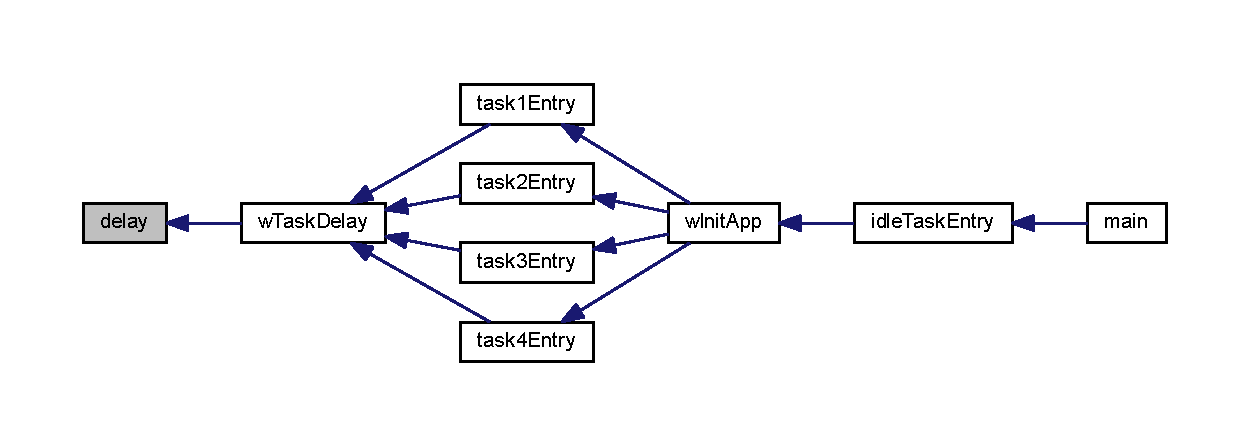
\includegraphics[width=350pt]{app_8c_a8eacdcdfdfb9ba0c6a62ee6206d0b1d4_icgraph}
\end{center}
\end{figure}
\mbox{\Hypertarget{app_8c_af8df096cffaabcd535dc2cdfb39a495f}\label{app_8c_af8df096cffaabcd535dc2cdfb39a495f}} 
\index{app.\+c@{app.\+c}!task1\+Entry@{task1\+Entry}}
\index{task1\+Entry@{task1\+Entry}!app.\+c@{app.\+c}}
\subsubsection{\texorpdfstring{task1\+Entry()}{task1Entry()}}
{\footnotesize\ttfamily void task1\+Entry (\begin{DoxyParamCaption}\item[{void $\ast$}]{param }\end{DoxyParamCaption})}



任务1入口函数 


\begin{DoxyParams}{参数}
{\em param:传给任务的参数} & \\
\hline
\end{DoxyParams}

\begin{DoxyRetVals}{返回值}
{\em 无} & \\
\hline
\end{DoxyRetVals}
函数调用图\+:
\nopagebreak
\begin{figure}[H]
\begin{center}
\leavevmode
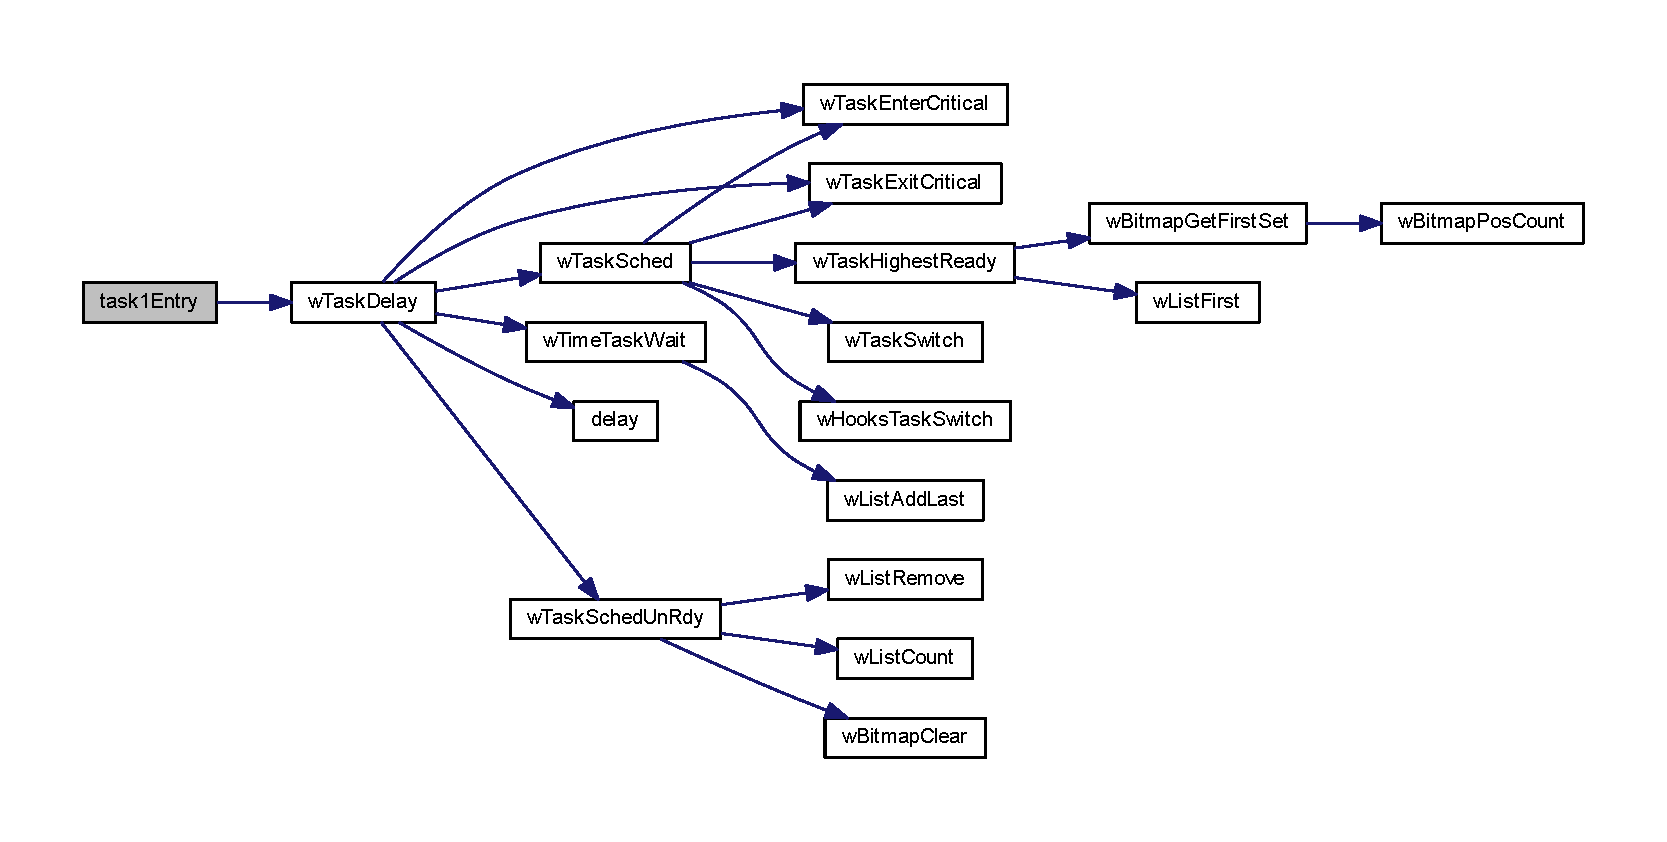
\includegraphics[width=350pt]{app_8c_af8df096cffaabcd535dc2cdfb39a495f_cgraph}
\end{center}
\end{figure}
这是这个函数的调用关系图\+:
\nopagebreak
\begin{figure}[H]
\begin{center}
\leavevmode
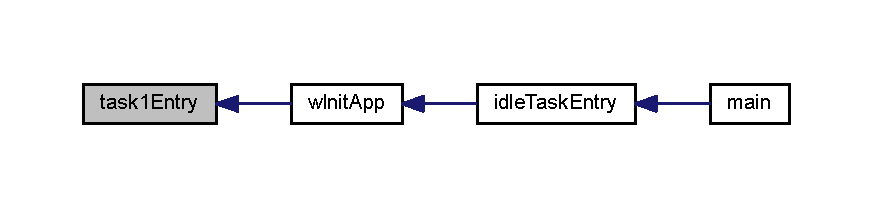
\includegraphics[width=350pt]{app_8c_af8df096cffaabcd535dc2cdfb39a495f_icgraph}
\end{center}
\end{figure}
\mbox{\Hypertarget{app_8c_a58232f2ac8acb8a9d60349af0fd7e8e2}\label{app_8c_a58232f2ac8acb8a9d60349af0fd7e8e2}} 
\index{app.\+c@{app.\+c}!task2\+Entry@{task2\+Entry}}
\index{task2\+Entry@{task2\+Entry}!app.\+c@{app.\+c}}
\subsubsection{\texorpdfstring{task2\+Entry()}{task2Entry()}}
{\footnotesize\ttfamily void task2\+Entry (\begin{DoxyParamCaption}\item[{void $\ast$}]{param }\end{DoxyParamCaption})}



任务2入口函数 


\begin{DoxyParams}{参数}
{\em param:传给任务的参数} & \\
\hline
\end{DoxyParams}

\begin{DoxyRetVals}{返回值}
{\em 无} & \\
\hline
\end{DoxyRetVals}
函数调用图\+:
\nopagebreak
\begin{figure}[H]
\begin{center}
\leavevmode
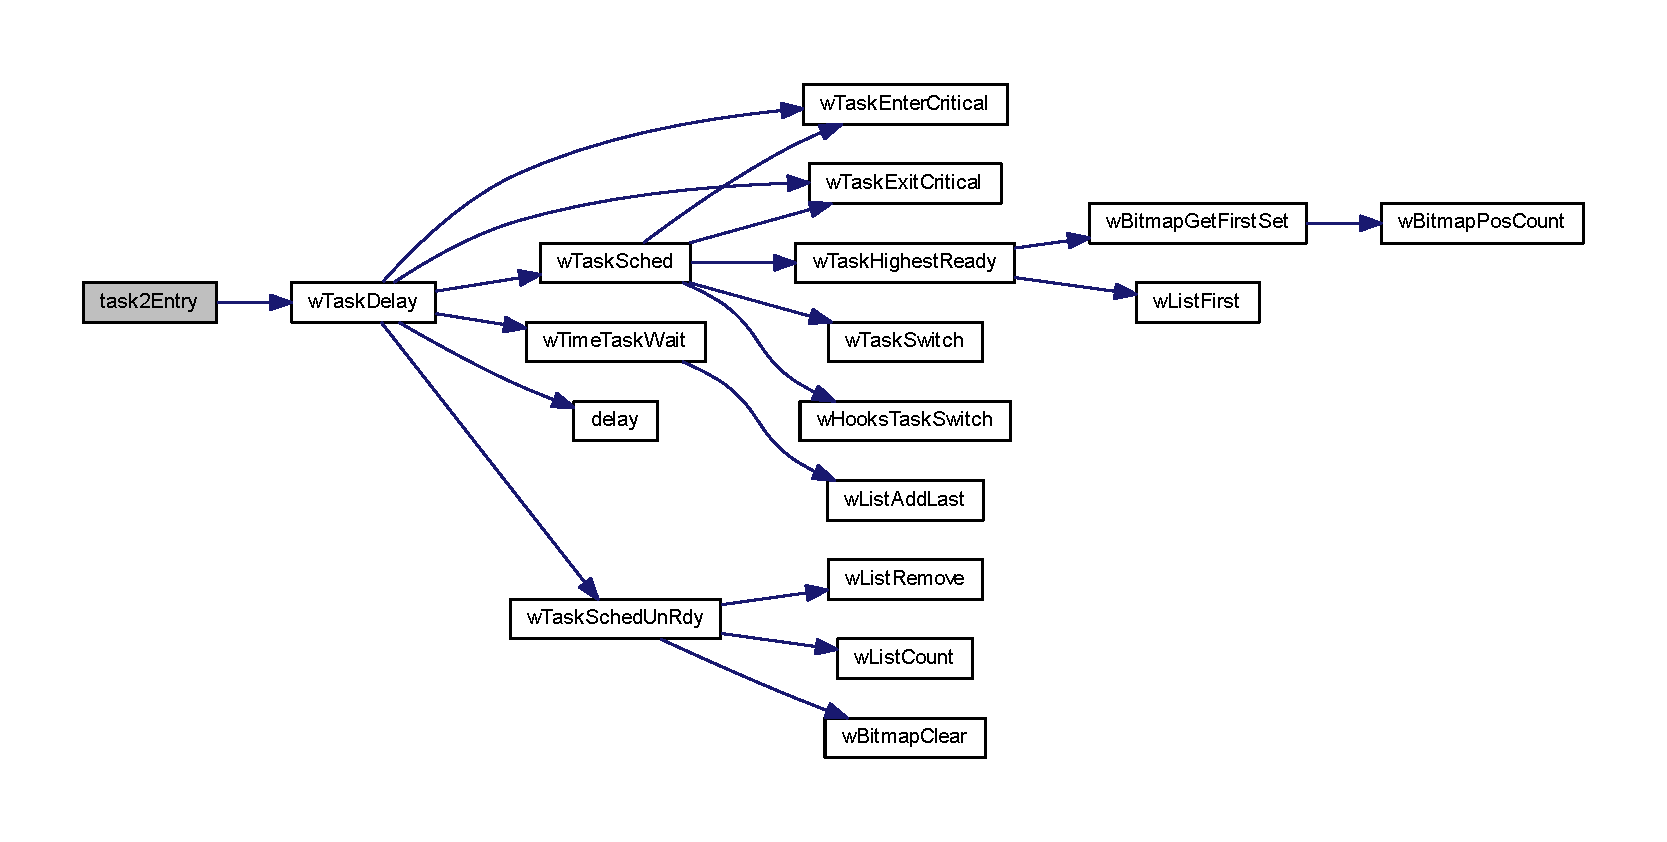
\includegraphics[width=350pt]{app_8c_a58232f2ac8acb8a9d60349af0fd7e8e2_cgraph}
\end{center}
\end{figure}
这是这个函数的调用关系图\+:
\nopagebreak
\begin{figure}[H]
\begin{center}
\leavevmode
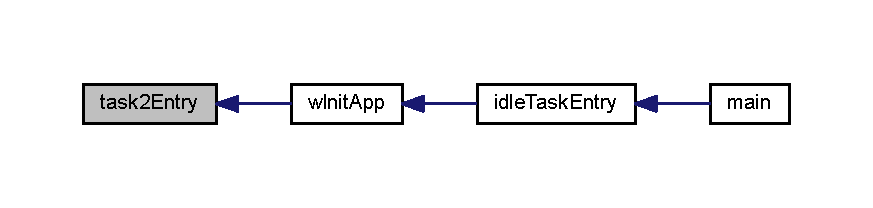
\includegraphics[width=350pt]{app_8c_a58232f2ac8acb8a9d60349af0fd7e8e2_icgraph}
\end{center}
\end{figure}
\mbox{\Hypertarget{app_8c_a771d21a21f591f1b9cdc8b2f834c4a7b}\label{app_8c_a771d21a21f591f1b9cdc8b2f834c4a7b}} 
\index{app.\+c@{app.\+c}!task3\+Entry@{task3\+Entry}}
\index{task3\+Entry@{task3\+Entry}!app.\+c@{app.\+c}}
\subsubsection{\texorpdfstring{task3\+Entry()}{task3Entry()}}
{\footnotesize\ttfamily void task3\+Entry (\begin{DoxyParamCaption}\item[{void $\ast$}]{param }\end{DoxyParamCaption})}



任务3入口函数 


\begin{DoxyParams}{参数}
{\em param:传给任务的参数} & \\
\hline
\end{DoxyParams}

\begin{DoxyRetVals}{返回值}
{\em 无} & \\
\hline
\end{DoxyRetVals}
函数调用图\+:
\nopagebreak
\begin{figure}[H]
\begin{center}
\leavevmode
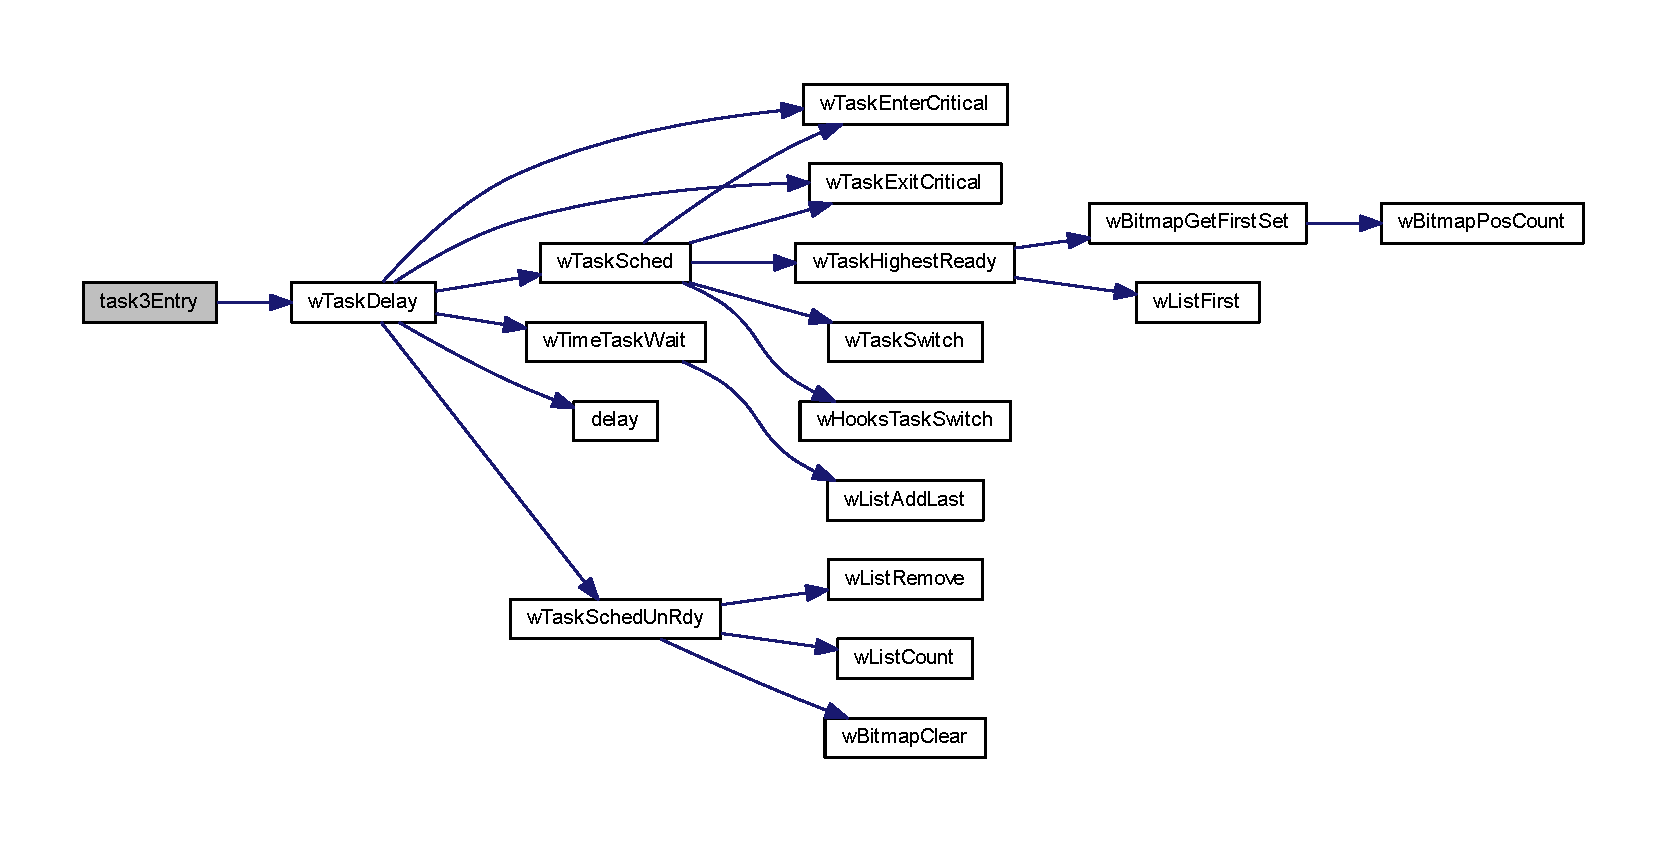
\includegraphics[width=350pt]{app_8c_a771d21a21f591f1b9cdc8b2f834c4a7b_cgraph}
\end{center}
\end{figure}
这是这个函数的调用关系图\+:
\nopagebreak
\begin{figure}[H]
\begin{center}
\leavevmode
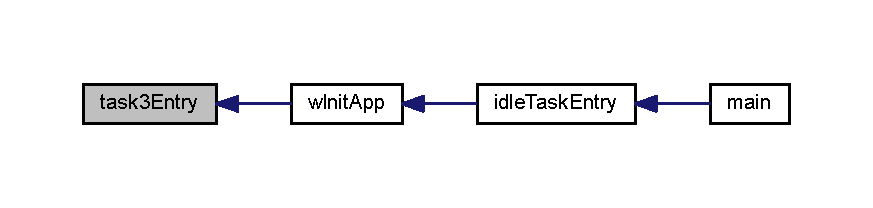
\includegraphics[width=350pt]{app_8c_a771d21a21f591f1b9cdc8b2f834c4a7b_icgraph}
\end{center}
\end{figure}
\mbox{\Hypertarget{app_8c_afe228a3d2729e128c20c88e66a0de25a}\label{app_8c_afe228a3d2729e128c20c88e66a0de25a}} 
\index{app.\+c@{app.\+c}!task4\+Entry@{task4\+Entry}}
\index{task4\+Entry@{task4\+Entry}!app.\+c@{app.\+c}}
\subsubsection{\texorpdfstring{task4\+Entry()}{task4Entry()}}
{\footnotesize\ttfamily void task4\+Entry (\begin{DoxyParamCaption}\item[{void $\ast$}]{param }\end{DoxyParamCaption})}



任务4入口函数 


\begin{DoxyParams}{参数}
{\em param:传给任务的参数} & \\
\hline
\end{DoxyParams}

\begin{DoxyRetVals}{返回值}
{\em 无} & \\
\hline
\end{DoxyRetVals}
函数调用图\+:
\nopagebreak
\begin{figure}[H]
\begin{center}
\leavevmode
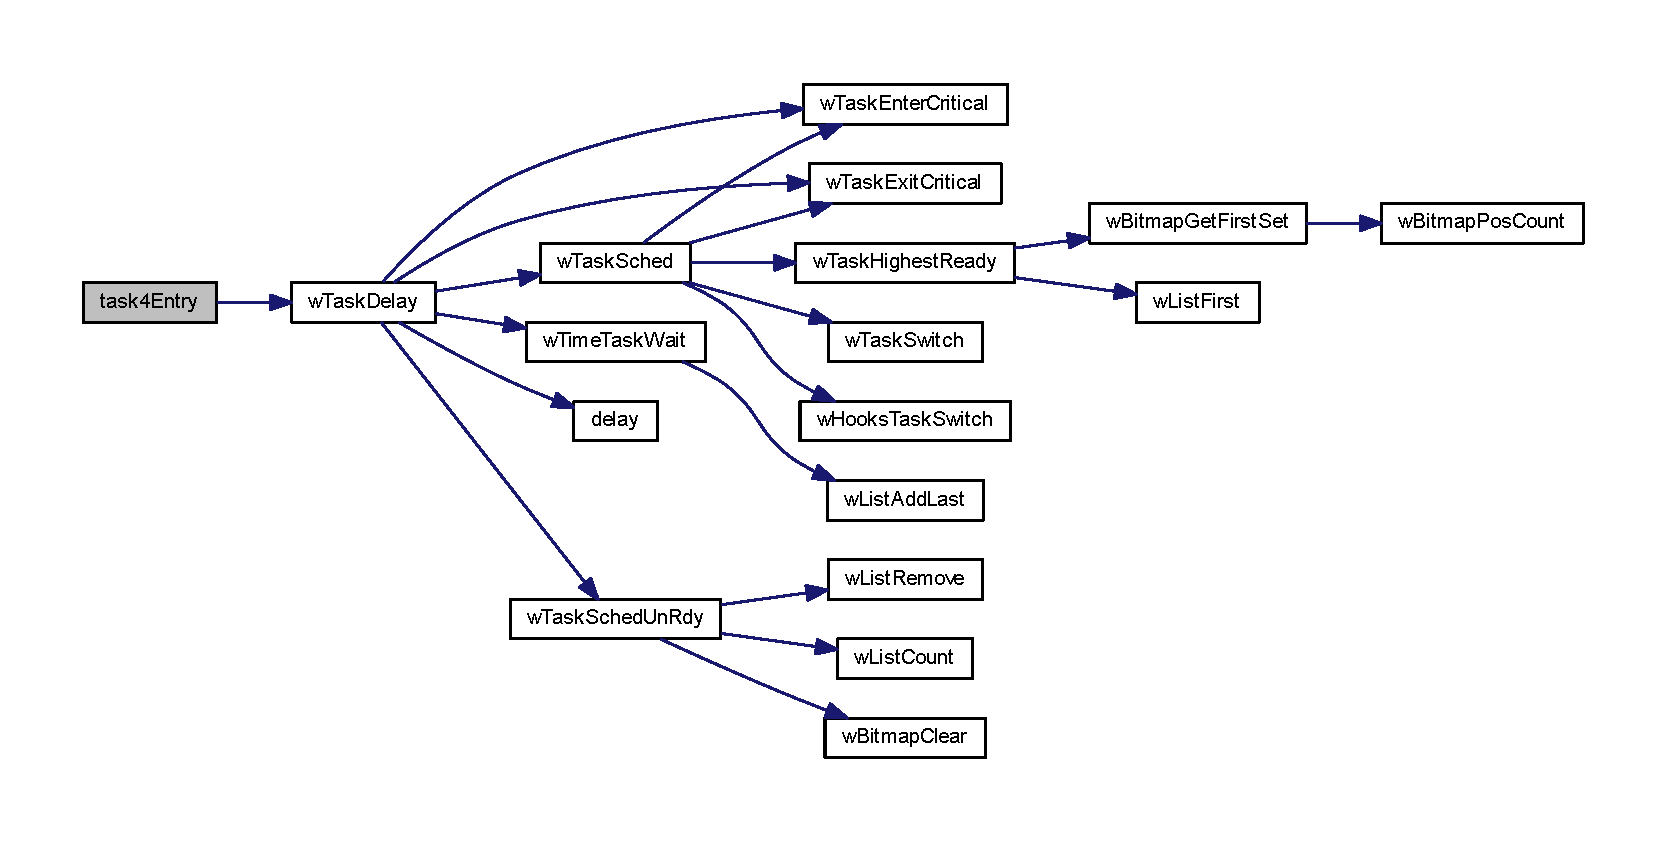
\includegraphics[width=350pt]{app_8c_afe228a3d2729e128c20c88e66a0de25a_cgraph}
\end{center}
\end{figure}
这是这个函数的调用关系图\+:
\nopagebreak
\begin{figure}[H]
\begin{center}
\leavevmode
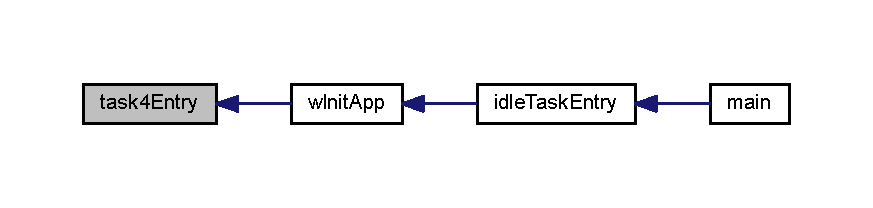
\includegraphics[width=350pt]{app_8c_afe228a3d2729e128c20c88e66a0de25a_icgraph}
\end{center}
\end{figure}
\mbox{\Hypertarget{app_8c_a01fa04097be631417a34fc2b5de3441a}\label{app_8c_a01fa04097be631417a34fc2b5de3441a}} 
\index{app.\+c@{app.\+c}!w\+Init\+App@{w\+Init\+App}}
\index{w\+Init\+App@{w\+Init\+App}!app.\+c@{app.\+c}}
\subsubsection{\texorpdfstring{w\+Init\+App()}{wInitApp()}}
{\footnotesize\ttfamily void w\+Init\+App (\begin{DoxyParamCaption}\item[{void}]{ }\end{DoxyParamCaption})}



任务初始化函数 


\begin{DoxyParams}{参数}
{\em 无} & \\
\hline
\end{DoxyParams}

\begin{DoxyRetVals}{返回值}
{\em 无} & \\
\hline
\end{DoxyRetVals}
函数调用图\+:
\nopagebreak
\begin{figure}[H]
\begin{center}
\leavevmode
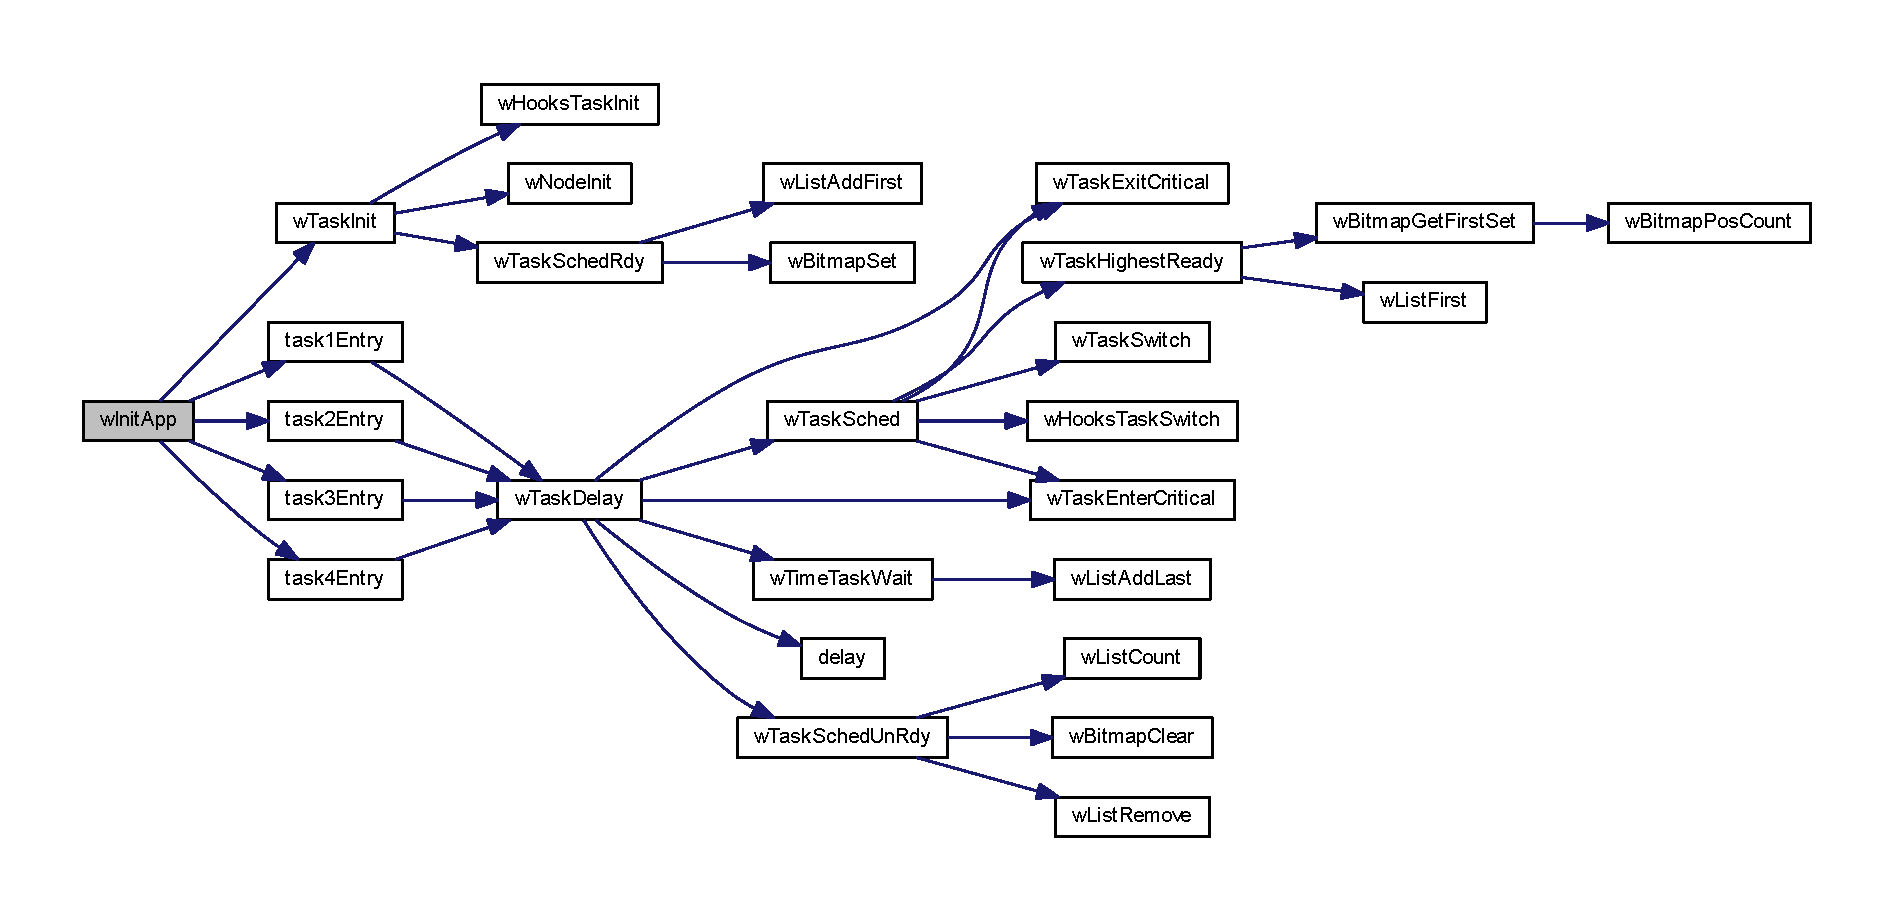
\includegraphics[width=350pt]{app_8c_a01fa04097be631417a34fc2b5de3441a_cgraph}
\end{center}
\end{figure}
这是这个函数的调用关系图\+:
\nopagebreak
\begin{figure}[H]
\begin{center}
\leavevmode
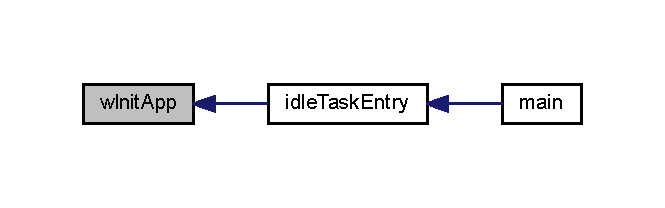
\includegraphics[width=319pt]{app_8c_a01fa04097be631417a34fc2b5de3441a_icgraph}
\end{center}
\end{figure}


\subsection{变量说明}
\mbox{\Hypertarget{app_8c_a5748ce11fa93ad0bd2caf38e20d9f46a}\label{app_8c_a5748ce11fa93ad0bd2caf38e20d9f46a}} 
\index{app.\+c@{app.\+c}!Task1\+Env@{Task1\+Env}}
\index{Task1\+Env@{Task1\+Env}!app.\+c@{app.\+c}}
\subsubsection{\texorpdfstring{Task1\+Env}{Task1Env}}
{\footnotesize\ttfamily \mbox{\hyperlink{w_task_8h_ae1dd34929f40dd21d0ea81f2d3f1c2e0}{w\+Task\+Stack}} Task1\+Env\mbox{[}1024\mbox{]}}

\mbox{\Hypertarget{app_8c_ad9cda71fc70dc1a2c00cc6e2c34df5af}\label{app_8c_ad9cda71fc70dc1a2c00cc6e2c34df5af}} 
\index{app.\+c@{app.\+c}!task1\+Flag@{task1\+Flag}}
\index{task1\+Flag@{task1\+Flag}!app.\+c@{app.\+c}}
\subsubsection{\texorpdfstring{task1\+Flag}{task1Flag}}
{\footnotesize\ttfamily int task1\+Flag}

\mbox{\Hypertarget{app_8c_a3228f67bea2c914f9e32333ed07a165f}\label{app_8c_a3228f67bea2c914f9e32333ed07a165f}} 
\index{app.\+c@{app.\+c}!Task2\+Env@{Task2\+Env}}
\index{Task2\+Env@{Task2\+Env}!app.\+c@{app.\+c}}
\subsubsection{\texorpdfstring{Task2\+Env}{Task2Env}}
{\footnotesize\ttfamily \mbox{\hyperlink{w_task_8h_ae1dd34929f40dd21d0ea81f2d3f1c2e0}{w\+Task\+Stack}} Task2\+Env\mbox{[}1024\mbox{]}}

\mbox{\Hypertarget{app_8c_aee561f6d9d7701291dc07ed736264942}\label{app_8c_aee561f6d9d7701291dc07ed736264942}} 
\index{app.\+c@{app.\+c}!task2\+Flag@{task2\+Flag}}
\index{task2\+Flag@{task2\+Flag}!app.\+c@{app.\+c}}
\subsubsection{\texorpdfstring{task2\+Flag}{task2Flag}}
{\footnotesize\ttfamily int task2\+Flag}

\mbox{\Hypertarget{app_8c_a71e290c848fe4fe968c811cc1ef1c46b}\label{app_8c_a71e290c848fe4fe968c811cc1ef1c46b}} 
\index{app.\+c@{app.\+c}!Task3\+Env@{Task3\+Env}}
\index{Task3\+Env@{Task3\+Env}!app.\+c@{app.\+c}}
\subsubsection{\texorpdfstring{Task3\+Env}{Task3Env}}
{\footnotesize\ttfamily \mbox{\hyperlink{w_task_8h_ae1dd34929f40dd21d0ea81f2d3f1c2e0}{w\+Task\+Stack}} Task3\+Env\mbox{[}1024\mbox{]}}

\mbox{\Hypertarget{app_8c_a421a992fc3f38902de45cf746516b7f6}\label{app_8c_a421a992fc3f38902de45cf746516b7f6}} 
\index{app.\+c@{app.\+c}!task3\+Flag@{task3\+Flag}}
\index{task3\+Flag@{task3\+Flag}!app.\+c@{app.\+c}}
\subsubsection{\texorpdfstring{task3\+Flag}{task3Flag}}
{\footnotesize\ttfamily int task3\+Flag}

\mbox{\Hypertarget{app_8c_ad3dd75e9a7c1bca3a5f1cc41aecf13a0}\label{app_8c_ad3dd75e9a7c1bca3a5f1cc41aecf13a0}} 
\index{app.\+c@{app.\+c}!Task4\+Env@{Task4\+Env}}
\index{Task4\+Env@{Task4\+Env}!app.\+c@{app.\+c}}
\subsubsection{\texorpdfstring{Task4\+Env}{Task4Env}}
{\footnotesize\ttfamily \mbox{\hyperlink{w_task_8h_ae1dd34929f40dd21d0ea81f2d3f1c2e0}{w\+Task\+Stack}} Task4\+Env\mbox{[}1024\mbox{]}}

\mbox{\Hypertarget{app_8c_afd6a73505313e637d637b9887894b2a8}\label{app_8c_afd6a73505313e637d637b9887894b2a8}} 
\index{app.\+c@{app.\+c}!task4\+Flag@{task4\+Flag}}
\index{task4\+Flag@{task4\+Flag}!app.\+c@{app.\+c}}
\subsubsection{\texorpdfstring{task4\+Flag}{task4Flag}}
{\footnotesize\ttfamily int task4\+Flag}

\mbox{\Hypertarget{app_8c_a4712a28475b04585701eb7f2a0050581}\label{app_8c_a4712a28475b04585701eb7f2a0050581}} 
\index{app.\+c@{app.\+c}!w\+Task1@{w\+Task1}}
\index{w\+Task1@{w\+Task1}!app.\+c@{app.\+c}}
\subsubsection{\texorpdfstring{w\+Task1}{wTask1}}
{\footnotesize\ttfamily \mbox{\hyperlink{w_task_8h_acd0e6238476f631a6ac4588629bac372}{w\+Task}} w\+Task1}

\mbox{\Hypertarget{app_8c_ab9f2aab5dabeeef56286973a4195feb4}\label{app_8c_ab9f2aab5dabeeef56286973a4195feb4}} 
\index{app.\+c@{app.\+c}!w\+Task2@{w\+Task2}}
\index{w\+Task2@{w\+Task2}!app.\+c@{app.\+c}}
\subsubsection{\texorpdfstring{w\+Task2}{wTask2}}
{\footnotesize\ttfamily \mbox{\hyperlink{w_task_8h_acd0e6238476f631a6ac4588629bac372}{w\+Task}} w\+Task2}

\mbox{\Hypertarget{app_8c_ab9dc37c449a10dd700b08f218f7ec2d3}\label{app_8c_ab9dc37c449a10dd700b08f218f7ec2d3}} 
\index{app.\+c@{app.\+c}!w\+Task3@{w\+Task3}}
\index{w\+Task3@{w\+Task3}!app.\+c@{app.\+c}}
\subsubsection{\texorpdfstring{w\+Task3}{wTask3}}
{\footnotesize\ttfamily \mbox{\hyperlink{w_task_8h_acd0e6238476f631a6ac4588629bac372}{w\+Task}} w\+Task3}

\mbox{\Hypertarget{app_8c_a942791273dec5ba24f2c36a6db1c8955}\label{app_8c_a942791273dec5ba24f2c36a6db1c8955}} 
\index{app.\+c@{app.\+c}!w\+Task4@{w\+Task4}}
\index{w\+Task4@{w\+Task4}!app.\+c@{app.\+c}}
\subsubsection{\texorpdfstring{w\+Task4}{wTask4}}
{\footnotesize\ttfamily \mbox{\hyperlink{w_task_8h_acd0e6238476f631a6ac4588629bac372}{w\+Task}} w\+Task4}


\hypertarget{main_8c}{}\section{C\+:/\+Users/pc/\+Desktop/\+W\+Q\+\_\+\+O\+S/\+Project/\+Sourse/main.c 文件参考}
\label{main_8c}\index{C\+:/\+Users/pc/\+Desktop/\+W\+Q\+\_\+\+O\+S/\+Project/\+Sourse/main.\+c@{C\+:/\+Users/pc/\+Desktop/\+W\+Q\+\_\+\+O\+S/\+Project/\+Sourse/main.\+c}}
{\ttfamily \#include \char`\"{}W\+Q\+\_\+\+O\+S.\+h\char`\"{}}\newline
{\ttfamily \#include $<$A\+R\+M\+C\+M3.\+h$>$}\newline
main.\+c 的引用(Include)关系图\+:
\nopagebreak
\begin{figure}[H]
\begin{center}
\leavevmode
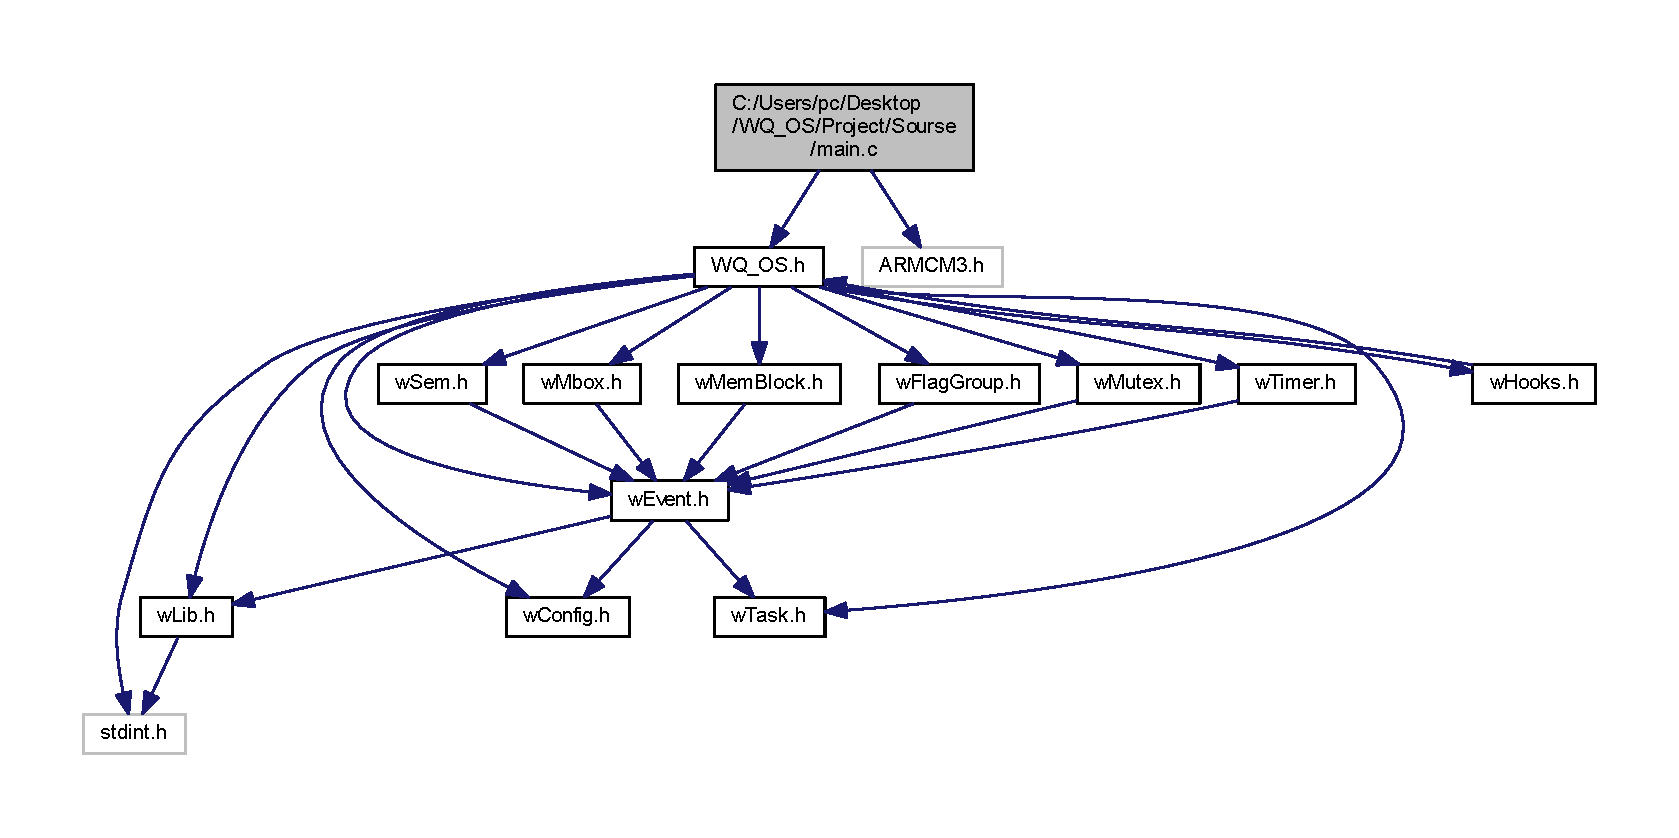
\includegraphics[width=350pt]{main_8c__incl}
\end{center}
\end{figure}
\subsection*{函数}
\begin{DoxyCompactItemize}
\item 
static void \mbox{\hyperlink{main_8c_a71898b6fe71a66a9230dd5a1b7c75521}{init\+Cpu\+Usage\+Stat}} (void)
\begin{DoxyCompactList}\small\item\em 初始化\+C\+P\+U统计函数 \end{DoxyCompactList}\item 
static void \mbox{\hyperlink{main_8c_a80aff2f9f799b816897b10c0c3fe700f}{check\+Cpu\+Usage}} (void)
\begin{DoxyCompactList}\small\item\em 检查\+C\+P\+U使用率函数 \end{DoxyCompactList}\item 
static void \mbox{\hyperlink{main_8c_ada21b0376c48e6165a98ba2f26a8ce59}{cpu\+Usage\+Sync\+With\+Sys\+Tick}} (void)
\begin{DoxyCompactList}\small\item\em 等待时钟同步函数 \end{DoxyCompactList}\item 
\mbox{\hyperlink{w_task_8h_acd0e6238476f631a6ac4588629bac372}{w\+Task}} $\ast$ \mbox{\hyperlink{main_8c_aecc5337584ee14a8c816f9ce689ba128}{w\+Task\+Highest\+Ready}} (void)
\begin{DoxyCompactList}\small\item\em 获取当前最高优先级且可运行的任务函数 \end{DoxyCompactList}\item 
void \mbox{\hyperlink{main_8c_a4d9a0f3090b684084bbe94f148747cd0}{w\+Task\+Sched\+Init}} (void)
\begin{DoxyCompactList}\small\item\em 内核初始化函数(初始化调度器) \end{DoxyCompactList}\item 
void \mbox{\hyperlink{main_8c_a033b0131d8e17bf2e857a743a02313f7}{w\+Task\+Sched\+Disable}} (void)
\begin{DoxyCompactList}\small\item\em 调度锁上锁函数 \end{DoxyCompactList}\item 
void \mbox{\hyperlink{main_8c_ae6dc919e0faa1e15e92c96899202c0a5}{w\+Task\+Sched\+Enable}} (void)
\begin{DoxyCompactList}\small\item\em 允许任务调度函数 \end{DoxyCompactList}\item 
void \mbox{\hyperlink{main_8c_a600f0ce279bbc48c121bd6e31874aff9}{w\+Task\+Sched\+Rdy}} (\mbox{\hyperlink{w_task_8h_acd0e6238476f631a6ac4588629bac372}{w\+Task}} $\ast$task)
\begin{DoxyCompactList}\small\item\em 将任务插入就绪列表(将任务从延时队列中移除时)函数 \end{DoxyCompactList}\item 
void \mbox{\hyperlink{main_8c_a598536b78a16c960ddfb82d887746cae}{w\+Task\+Sched\+Un\+Rdy}} (\mbox{\hyperlink{w_task_8h_acd0e6238476f631a6ac4588629bac372}{w\+Task}} $\ast$task)
\begin{DoxyCompactList}\small\item\em 将任务从就绪列表中删除函数 \end{DoxyCompactList}\item 
void \mbox{\hyperlink{main_8c_ad212054b17e4733e330c97f3d3274767}{w\+Task\+Sched\+Remove}} (\mbox{\hyperlink{w_task_8h_acd0e6238476f631a6ac4588629bac372}{w\+Task}} $\ast$task)
\begin{DoxyCompactList}\small\item\em 将任务从优先级列表中删除函数 \end{DoxyCompactList}\item 
void \mbox{\hyperlink{main_8c_a231177ae77d1af6c5239c4ca95be8760}{w\+Task\+Sched}} (void)
\begin{DoxyCompactList}\small\item\em 任务调度函数 \end{DoxyCompactList}\item 
void \mbox{\hyperlink{main_8c_a9198e3ccd3e666f8caf7587679165ef8}{w\+Task\+Delay\+Init}} (void)
\begin{DoxyCompactList}\small\item\em 任务延时初始化函数 \end{DoxyCompactList}\item 
void \mbox{\hyperlink{main_8c_a1163983eff6acb009950c69f3a55b629}{w\+Time\+Task\+Wait}} (\mbox{\hyperlink{w_task_8h_acd0e6238476f631a6ac4588629bac372}{w\+Task}} $\ast$task, uint32\+\_\+t ticks)
\begin{DoxyCompactList}\small\item\em 将任务插入延时队列函数 \end{DoxyCompactList}\item 
void \mbox{\hyperlink{main_8c_a85848b63b5fe499d55e6c4196c43f306}{w\+Time\+Task\+Wake\+Up}} (\mbox{\hyperlink{w_task_8h_acd0e6238476f631a6ac4588629bac372}{w\+Task}} $\ast$task)
\begin{DoxyCompactList}\small\item\em 将任务从延时队列唤醒函数 \end{DoxyCompactList}\item 
void \mbox{\hyperlink{main_8c_a135f5a694c1f6b01cb1499ecaf2ee0a5}{w\+Time\+Task\+Remove}} (\mbox{\hyperlink{w_task_8h_acd0e6238476f631a6ac4588629bac372}{w\+Task}} $\ast$task)
\begin{DoxyCompactList}\small\item\em 将任务从延时队列删除函数 \end{DoxyCompactList}\item 
void \mbox{\hyperlink{main_8c_ad2cede6eea6a293ae82a1cedb76bc6f3}{w\+Time\+Tick\+Init}} (void)
\begin{DoxyCompactList}\small\item\em 时钟节拍计数器初始化函数 \end{DoxyCompactList}\item 
void \mbox{\hyperlink{main_8c_a36ab31adb9bd20b1fe3337cf8ac6baf2}{w\+Task\+System\+Tick\+Handler}} (void)
\begin{DoxyCompactList}\small\item\em 任务\+System\+Tick中断服务函数 \end{DoxyCompactList}\item 
float \mbox{\hyperlink{main_8c_a741910b18aa077abc57d210e73d03465}{w\+Cpu\+Usage\+Get}} (void)
\begin{DoxyCompactList}\small\item\em 获取\+C\+P\+U使用率函数 \end{DoxyCompactList}\item 
void \mbox{\hyperlink{main_8c_a1949c76c0bc7d4b976d447fbaa947f53}{idle\+Task\+Entry}} (void $\ast$param)
\begin{DoxyCompactList}\small\item\em 空闲任务函数 \end{DoxyCompactList}\item 
int \mbox{\hyperlink{main_8c_ae66f6b31b5ad750f1fe042a706a4e3d4}{main}} ()
\begin{DoxyCompactList}\small\item\em 主函数 \end{DoxyCompactList}\end{DoxyCompactItemize}
\subsection*{变量}
\begin{DoxyCompactItemize}
\item 
\mbox{\hyperlink{w_task_8h_acd0e6238476f631a6ac4588629bac372}{w\+Task}} $\ast$ \mbox{\hyperlink{main_8c_a6bec055003640755e2481f3cf0692894}{current\+Task}}
\item 
\mbox{\hyperlink{w_task_8h_acd0e6238476f631a6ac4588629bac372}{w\+Task}} $\ast$ \mbox{\hyperlink{main_8c_a44a5b29a47ca1930c940bc88c9051e0e}{next\+Task}}
\item 
\mbox{\hyperlink{w_task_8h_acd0e6238476f631a6ac4588629bac372}{w\+Task}} $\ast$ \mbox{\hyperlink{main_8c_a23c0ee4b0c015f3388e9e2dde31c66bb}{idle\+Task}}
\item 
\mbox{\hyperlink{structw_bitmap}{w\+Bitmap}} \mbox{\hyperlink{main_8c_a59fae34e401c2e655eee7ffc8981189f}{task\+Prio\+Bitmap}}
\item 
\mbox{\hyperlink{w_lib_8h_a3f922f977222a1e1fc18bd2ce6d668c3}{w\+List}} \mbox{\hyperlink{main_8c_aad68ddf20dbfe94a640011019f2e2bbc}{task\+Table}} \mbox{[}\mbox{\hyperlink{w_config_8h_ac74e7af2bb0660ccb34d04ef1e5a48d2}{W\+Q\+\_\+\+O\+S\+\_\+\+P\+R\+O\+\_\+\+C\+O\+U\+NT}}\mbox{]}
\item 
uint8\+\_\+t \mbox{\hyperlink{main_8c_a9fcac63fa1ff9049d9b30424558b1d30}{schedlock\+Count}}
\item 
uint32\+\_\+t \mbox{\hyperlink{main_8c_af4fc7964f7a64a2a55f189f4533015f4}{tick\+Count}}
\item 
\mbox{\hyperlink{w_lib_8h_a3f922f977222a1e1fc18bd2ce6d668c3}{w\+List}} \mbox{\hyperlink{main_8c_a5fb74394eca3c48232b60346daa851b7}{w\+Task\+Delay\+List}}
\item 
uint32\+\_\+t \mbox{\hyperlink{main_8c_a9979e3c27f522bb6d13cff22efd2e488}{idle\+Count}}
\item 
uint32\+\_\+t \mbox{\hyperlink{main_8c_aba65b5ed5e394f5ca1f346b4a53364cf}{idle\+Max\+Count}}
\item 
static float \mbox{\hyperlink{main_8c_a4d3fcca6f9564b4467b34cfa39cd5310}{cpu\+Usage}}
\item 
static uint32\+\_\+t \mbox{\hyperlink{main_8c_ae640b280f11b1ff0b28135982bbac7f5}{enable\+Cpu\+Usage\+Stat}}
\item 
\mbox{\hyperlink{w_task_8h_acd0e6238476f631a6ac4588629bac372}{w\+Task}} \mbox{\hyperlink{main_8c_aa6ce5811e5fc82d1c0b0c9526e3ee2dc}{w\+Task\+Idle}}
\item 
\mbox{\hyperlink{w_task_8h_ae1dd34929f40dd21d0ea81f2d3f1c2e0}{w\+Task\+Stack}} \mbox{\hyperlink{main_8c_ad6edc236a894fc8b921be2739d43ff24}{idle\+Task\+Env}} \mbox{[}\mbox{\hyperlink{w_config_8h_a9991397c90242f684eb25692adbfdc77}{W\+Q\+\_\+\+O\+S\+\_\+\+I\+D\+L\+E\+T\+A\+S\+K\+\_\+\+S\+T\+A\+C\+K\+\_\+\+S\+I\+ZE}}\mbox{]}
\end{DoxyCompactItemize}


\subsection{函数说明}
\mbox{\Hypertarget{main_8c_a80aff2f9f799b816897b10c0c3fe700f}\label{main_8c_a80aff2f9f799b816897b10c0c3fe700f}} 
\index{main.\+c@{main.\+c}!check\+Cpu\+Usage@{check\+Cpu\+Usage}}
\index{check\+Cpu\+Usage@{check\+Cpu\+Usage}!main.\+c@{main.\+c}}
\subsubsection{\texorpdfstring{check\+Cpu\+Usage()}{checkCpuUsage()}}
{\footnotesize\ttfamily static void check\+Cpu\+Usage (\begin{DoxyParamCaption}\item[{void}]{ }\end{DoxyParamCaption})\hspace{0.3cm}{\ttfamily [static]}}



检查\+C\+P\+U使用率函数 


\begin{DoxyParams}{参数}
{\em 无} & \\
\hline
\end{DoxyParams}

\begin{DoxyRetVals}{返回值}
{\em 无} & \\
\hline
\end{DoxyRetVals}
函数调用图\+:
\nopagebreak
\begin{figure}[H]
\begin{center}
\leavevmode
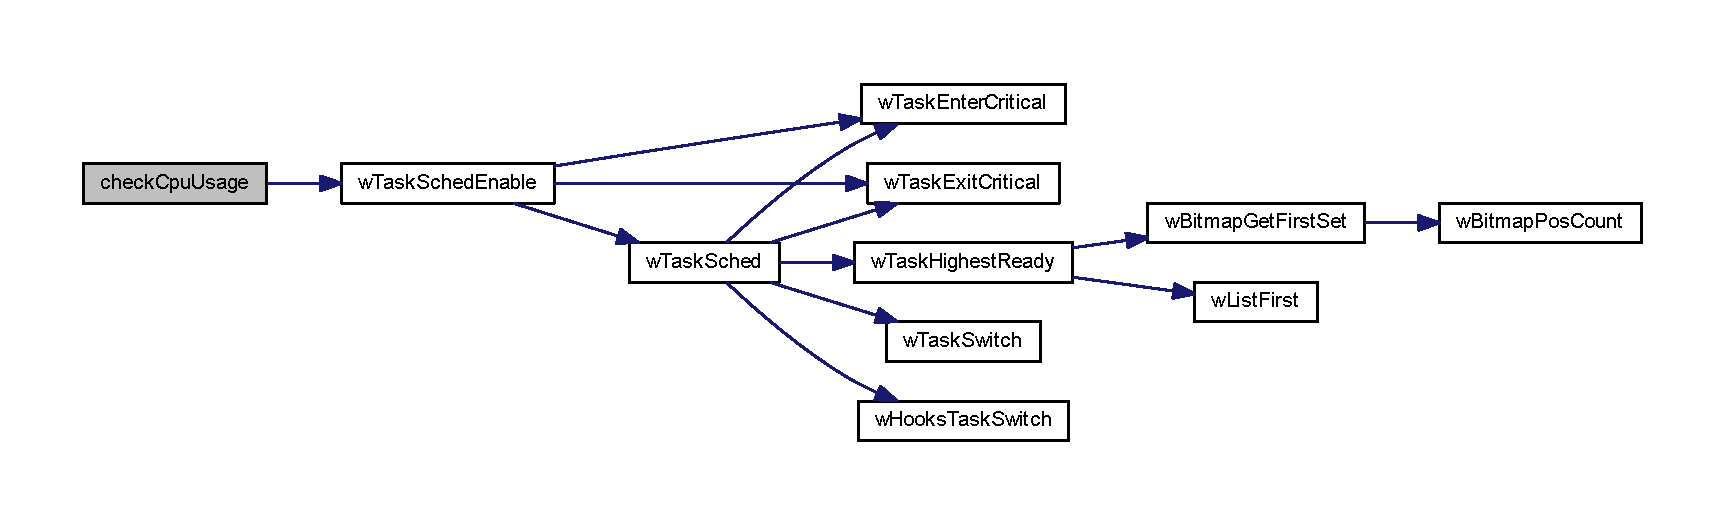
\includegraphics[width=350pt]{main_8c_a80aff2f9f799b816897b10c0c3fe700f_cgraph}
\end{center}
\end{figure}
这是这个函数的调用关系图\+:
\nopagebreak
\begin{figure}[H]
\begin{center}
\leavevmode
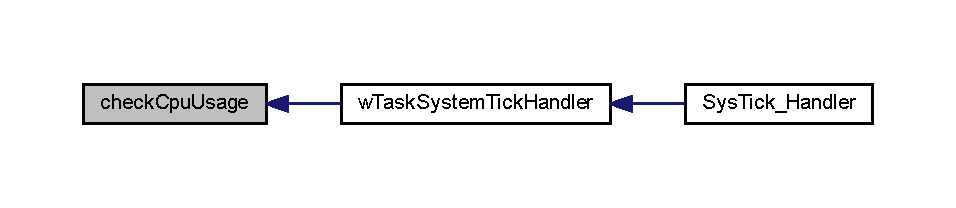
\includegraphics[width=350pt]{main_8c_a80aff2f9f799b816897b10c0c3fe700f_icgraph}
\end{center}
\end{figure}
\mbox{\Hypertarget{main_8c_ada21b0376c48e6165a98ba2f26a8ce59}\label{main_8c_ada21b0376c48e6165a98ba2f26a8ce59}} 
\index{main.\+c@{main.\+c}!cpu\+Usage\+Sync\+With\+Sys\+Tick@{cpu\+Usage\+Sync\+With\+Sys\+Tick}}
\index{cpu\+Usage\+Sync\+With\+Sys\+Tick@{cpu\+Usage\+Sync\+With\+Sys\+Tick}!main.\+c@{main.\+c}}
\subsubsection{\texorpdfstring{cpu\+Usage\+Sync\+With\+Sys\+Tick()}{cpuUsageSyncWithSysTick()}}
{\footnotesize\ttfamily static void cpu\+Usage\+Sync\+With\+Sys\+Tick (\begin{DoxyParamCaption}\item[{void}]{ }\end{DoxyParamCaption})\hspace{0.3cm}{\ttfamily [static]}}



等待时钟同步函数 


\begin{DoxyParams}{参数}
{\em 无} & \\
\hline
\end{DoxyParams}

\begin{DoxyRetVals}{返回值}
{\em 无} & \\
\hline
\end{DoxyRetVals}
这是这个函数的调用关系图\+:
\nopagebreak
\begin{figure}[H]
\begin{center}
\leavevmode
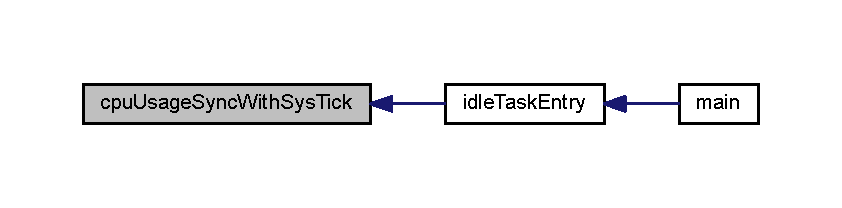
\includegraphics[width=350pt]{main_8c_ada21b0376c48e6165a98ba2f26a8ce59_icgraph}
\end{center}
\end{figure}
\mbox{\Hypertarget{main_8c_a1949c76c0bc7d4b976d447fbaa947f53}\label{main_8c_a1949c76c0bc7d4b976d447fbaa947f53}} 
\index{main.\+c@{main.\+c}!idle\+Task\+Entry@{idle\+Task\+Entry}}
\index{idle\+Task\+Entry@{idle\+Task\+Entry}!main.\+c@{main.\+c}}
\subsubsection{\texorpdfstring{idle\+Task\+Entry()}{idleTaskEntry()}}
{\footnotesize\ttfamily void idle\+Task\+Entry (\begin{DoxyParamCaption}\item[{void $\ast$}]{param }\end{DoxyParamCaption})}



空闲任务函数 


\begin{DoxyParams}{参数}
{\em 无} & \\
\hline
\end{DoxyParams}

\begin{DoxyRetVals}{返回值}
{\em 无} & \\
\hline
\end{DoxyRetVals}
函数调用图\+:
\nopagebreak
\begin{figure}[H]
\begin{center}
\leavevmode
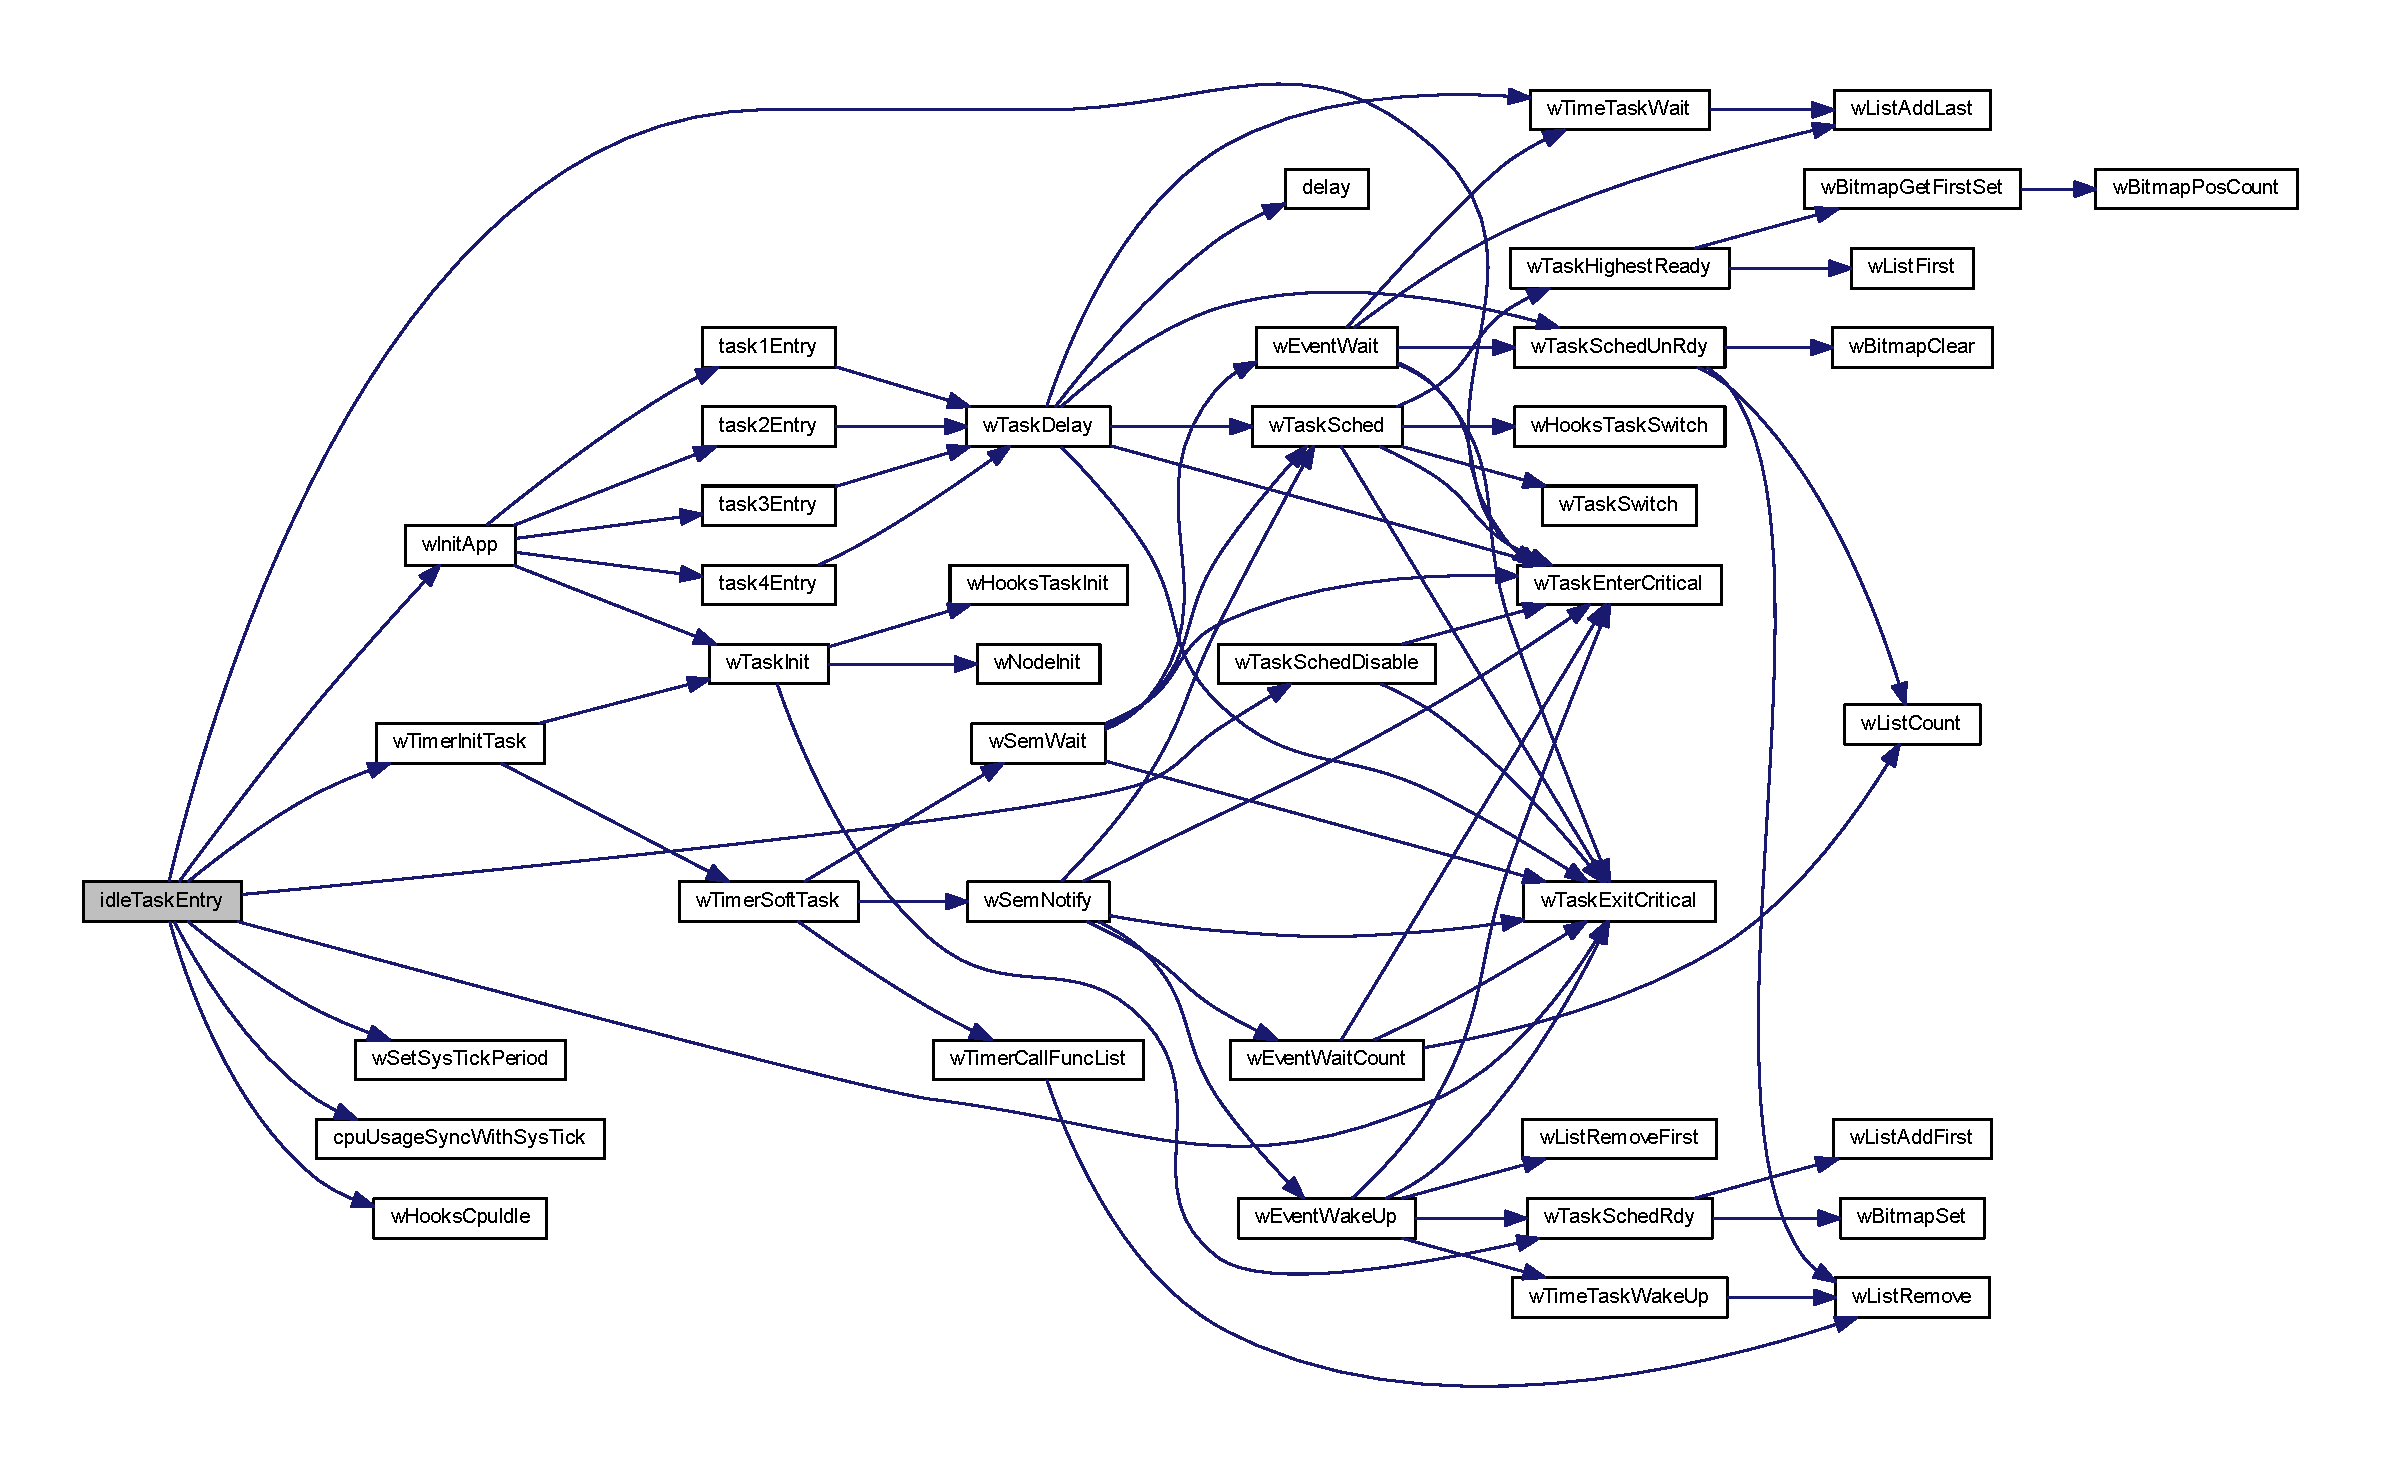
\includegraphics[width=350pt]{main_8c_a1949c76c0bc7d4b976d447fbaa947f53_cgraph}
\end{center}
\end{figure}
这是这个函数的调用关系图\+:
\nopagebreak
\begin{figure}[H]
\begin{center}
\leavevmode
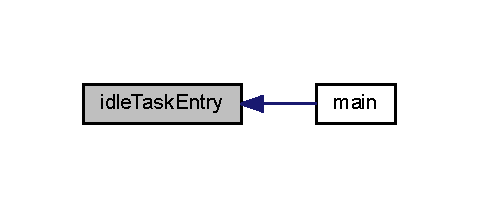
\includegraphics[width=230pt]{main_8c_a1949c76c0bc7d4b976d447fbaa947f53_icgraph}
\end{center}
\end{figure}
\mbox{\Hypertarget{main_8c_a71898b6fe71a66a9230dd5a1b7c75521}\label{main_8c_a71898b6fe71a66a9230dd5a1b7c75521}} 
\index{main.\+c@{main.\+c}!init\+Cpu\+Usage\+Stat@{init\+Cpu\+Usage\+Stat}}
\index{init\+Cpu\+Usage\+Stat@{init\+Cpu\+Usage\+Stat}!main.\+c@{main.\+c}}
\subsubsection{\texorpdfstring{init\+Cpu\+Usage\+Stat()}{initCpuUsageStat()}}
{\footnotesize\ttfamily static void init\+Cpu\+Usage\+Stat (\begin{DoxyParamCaption}\item[{void}]{ }\end{DoxyParamCaption})\hspace{0.3cm}{\ttfamily [static]}}



初始化\+C\+P\+U统计函数 


\begin{DoxyParams}{参数}
{\em 无} & \\
\hline
\end{DoxyParams}

\begin{DoxyRetVals}{返回值}
{\em 无} & \\
\hline
\end{DoxyRetVals}
这是这个函数的调用关系图\+:
\nopagebreak
\begin{figure}[H]
\begin{center}
\leavevmode
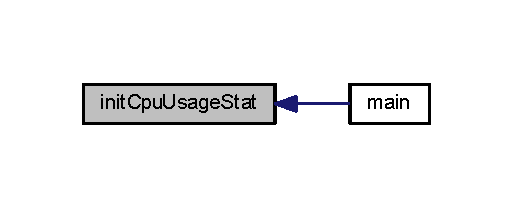
\includegraphics[width=246pt]{main_8c_a71898b6fe71a66a9230dd5a1b7c75521_icgraph}
\end{center}
\end{figure}
\mbox{\Hypertarget{main_8c_ae66f6b31b5ad750f1fe042a706a4e3d4}\label{main_8c_ae66f6b31b5ad750f1fe042a706a4e3d4}} 
\index{main.\+c@{main.\+c}!main@{main}}
\index{main@{main}!main.\+c@{main.\+c}}
\subsubsection{\texorpdfstring{main()}{main()}}
{\footnotesize\ttfamily int main (\begin{DoxyParamCaption}{ }\end{DoxyParamCaption})}



主函数 


\begin{DoxyParams}{参数}
{\em 无} & \\
\hline
\end{DoxyParams}

\begin{DoxyRetVals}{返回值}
{\em 无} & \\
\hline
\end{DoxyRetVals}
函数调用图\+:
\nopagebreak
\begin{figure}[H]
\begin{center}
\leavevmode
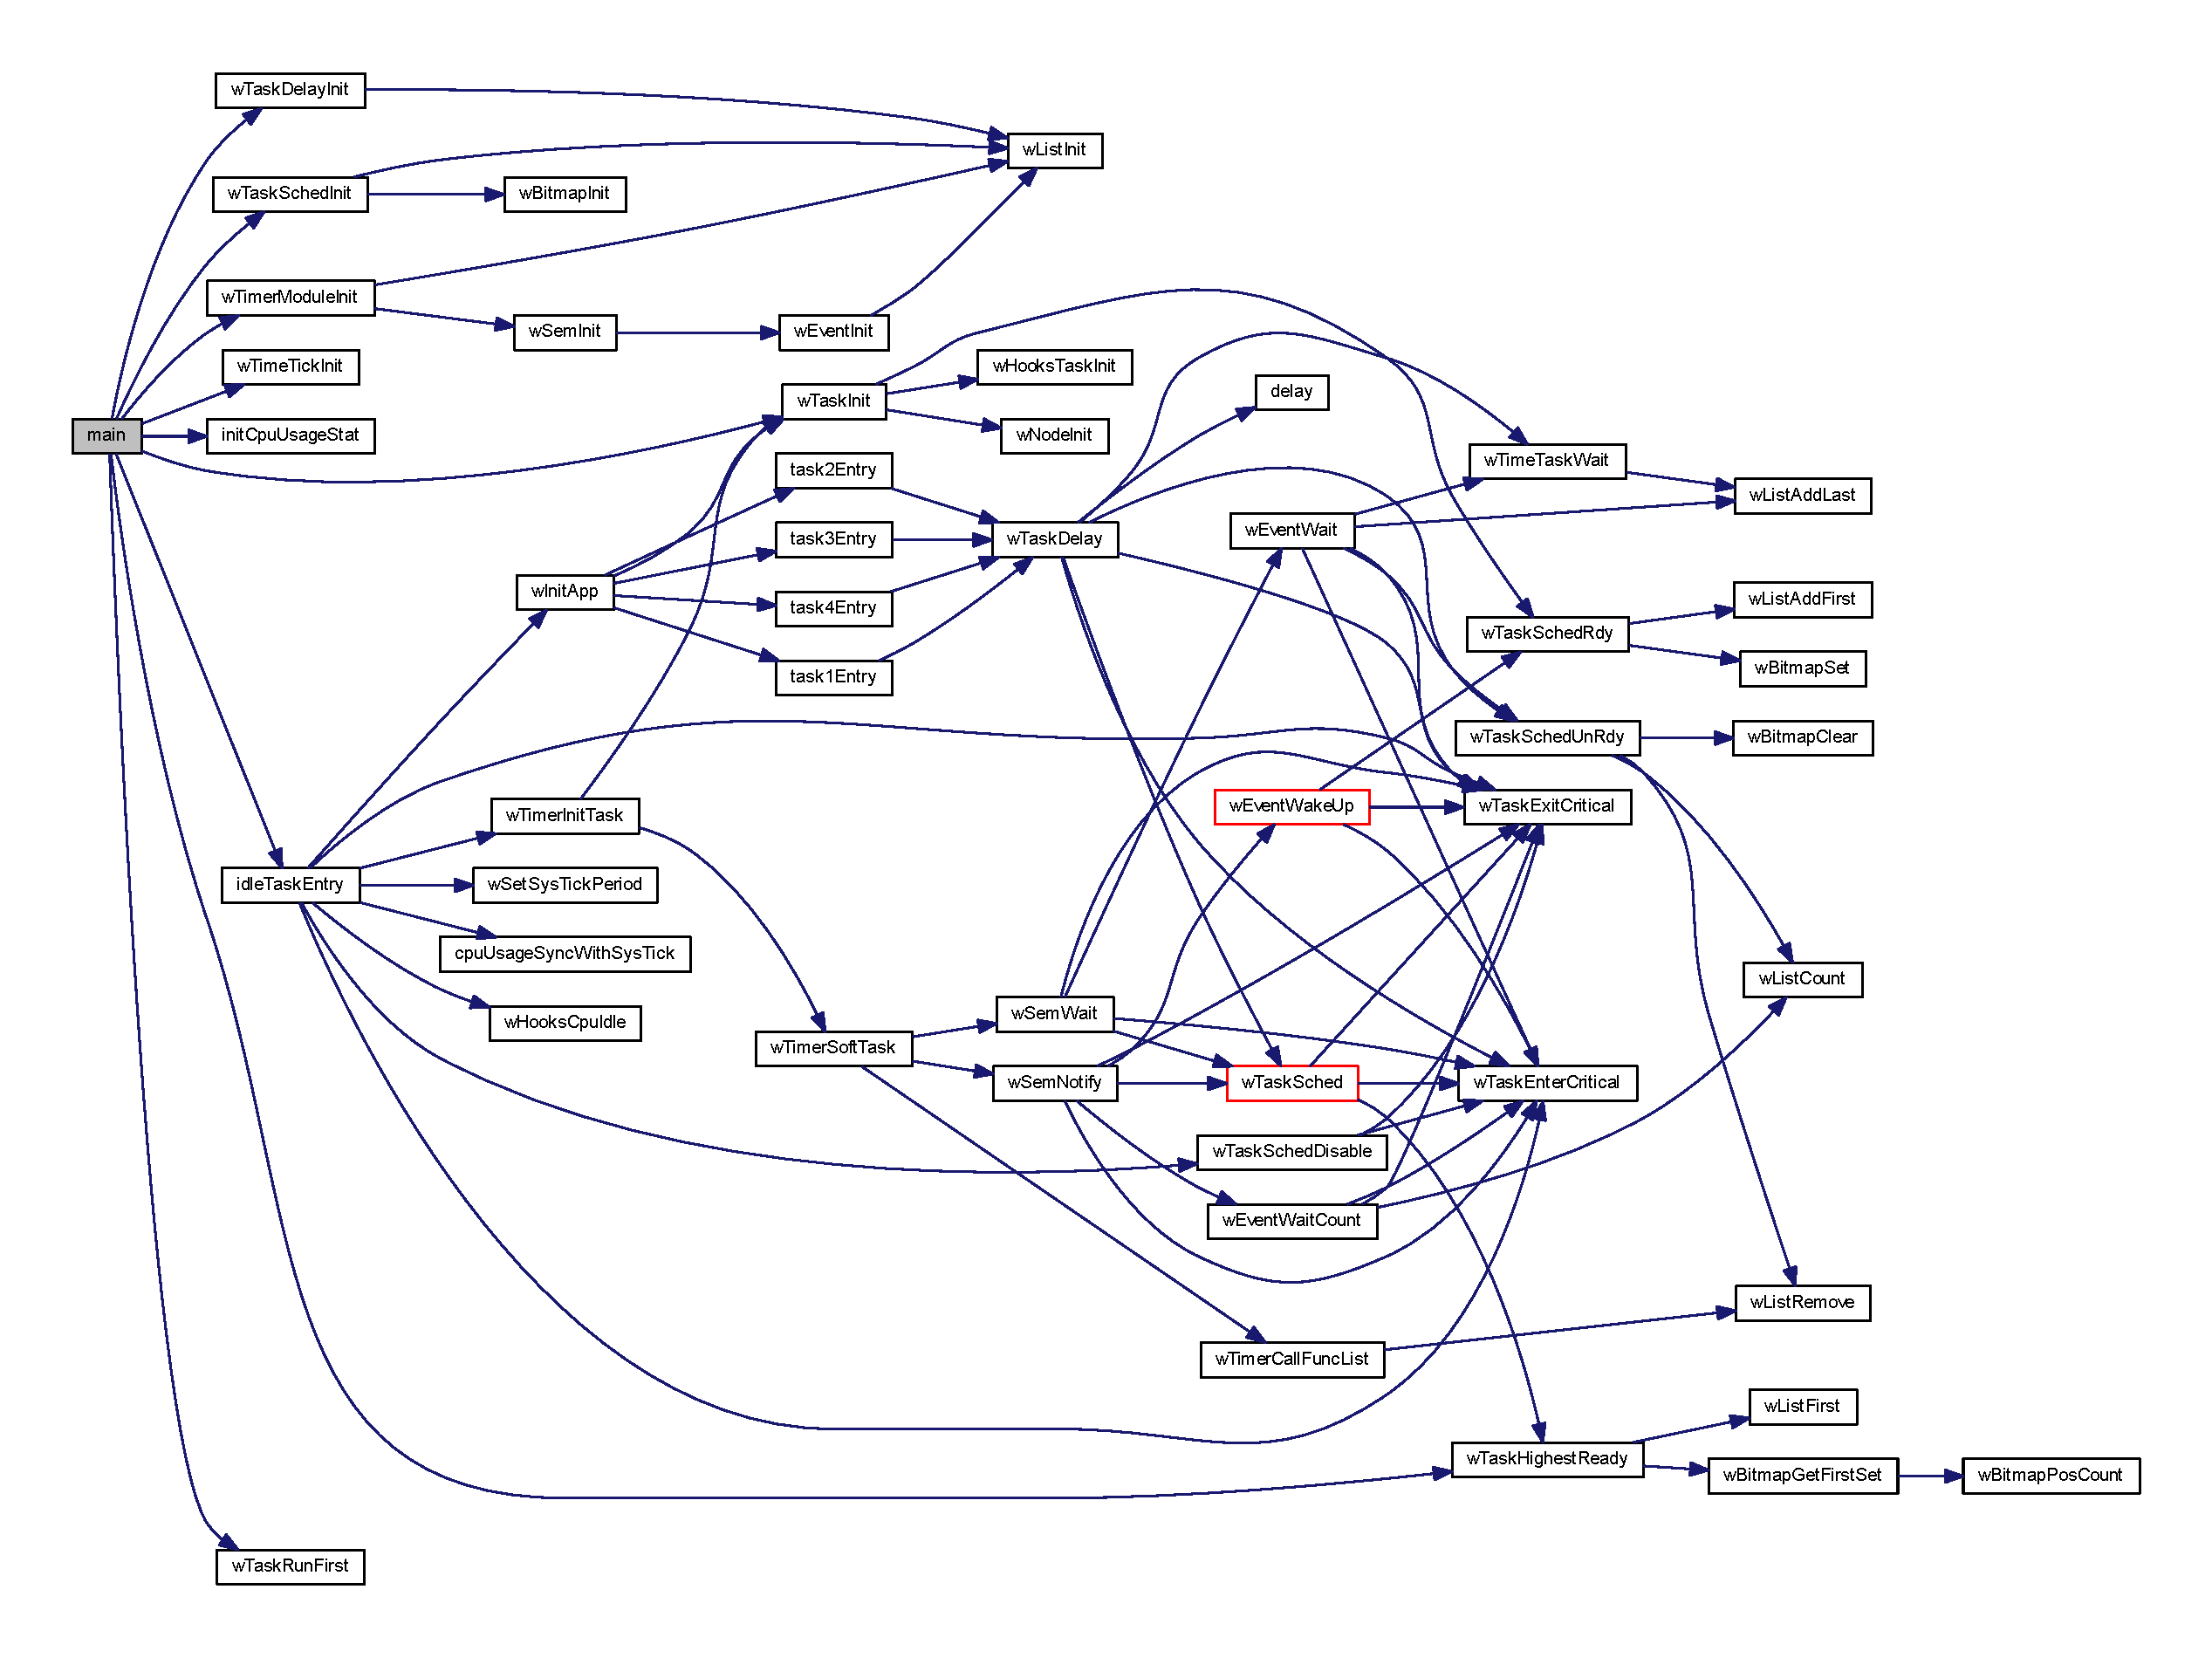
\includegraphics[width=350pt]{main_8c_ae66f6b31b5ad750f1fe042a706a4e3d4_cgraph}
\end{center}
\end{figure}
\mbox{\Hypertarget{main_8c_a741910b18aa077abc57d210e73d03465}\label{main_8c_a741910b18aa077abc57d210e73d03465}} 
\index{main.\+c@{main.\+c}!w\+Cpu\+Usage\+Get@{w\+Cpu\+Usage\+Get}}
\index{w\+Cpu\+Usage\+Get@{w\+Cpu\+Usage\+Get}!main.\+c@{main.\+c}}
\subsubsection{\texorpdfstring{w\+Cpu\+Usage\+Get()}{wCpuUsageGet()}}
{\footnotesize\ttfamily float w\+Cpu\+Usage\+Get (\begin{DoxyParamCaption}\item[{void}]{ }\end{DoxyParamCaption})}



获取\+C\+P\+U使用率函数 


\begin{DoxyParams}{参数}
{\em 无} & \\
\hline
\end{DoxyParams}

\begin{DoxyRetVals}{返回值}
{\em C\+P\+U使用率} & \\
\hline
\end{DoxyRetVals}
函数调用图\+:
\nopagebreak
\begin{figure}[H]
\begin{center}
\leavevmode
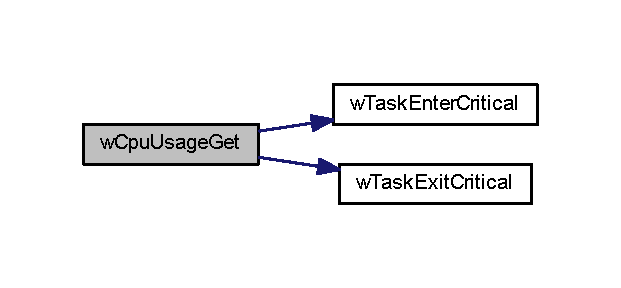
\includegraphics[width=298pt]{main_8c_a741910b18aa077abc57d210e73d03465_cgraph}
\end{center}
\end{figure}
\mbox{\Hypertarget{main_8c_a9198e3ccd3e666f8caf7587679165ef8}\label{main_8c_a9198e3ccd3e666f8caf7587679165ef8}} 
\index{main.\+c@{main.\+c}!w\+Task\+Delay\+Init@{w\+Task\+Delay\+Init}}
\index{w\+Task\+Delay\+Init@{w\+Task\+Delay\+Init}!main.\+c@{main.\+c}}
\subsubsection{\texorpdfstring{w\+Task\+Delay\+Init()}{wTaskDelayInit()}}
{\footnotesize\ttfamily void w\+Task\+Delay\+Init (\begin{DoxyParamCaption}\item[{void}]{ }\end{DoxyParamCaption})}



任务延时初始化函数 


\begin{DoxyParams}{参数}
{\em 无} & \\
\hline
\end{DoxyParams}

\begin{DoxyRetVals}{返回值}
{\em 无} & \\
\hline
\end{DoxyRetVals}
函数调用图\+:
\nopagebreak
\begin{figure}[H]
\begin{center}
\leavevmode
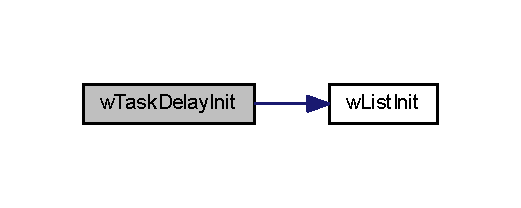
\includegraphics[width=250pt]{main_8c_a9198e3ccd3e666f8caf7587679165ef8_cgraph}
\end{center}
\end{figure}
这是这个函数的调用关系图\+:
\nopagebreak
\begin{figure}[H]
\begin{center}
\leavevmode
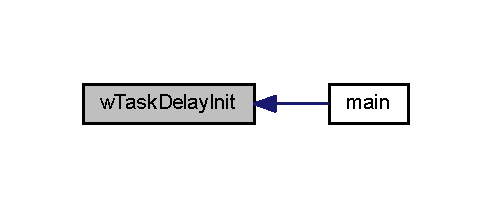
\includegraphics[width=236pt]{main_8c_a9198e3ccd3e666f8caf7587679165ef8_icgraph}
\end{center}
\end{figure}
\mbox{\Hypertarget{main_8c_aecc5337584ee14a8c816f9ce689ba128}\label{main_8c_aecc5337584ee14a8c816f9ce689ba128}} 
\index{main.\+c@{main.\+c}!w\+Task\+Highest\+Ready@{w\+Task\+Highest\+Ready}}
\index{w\+Task\+Highest\+Ready@{w\+Task\+Highest\+Ready}!main.\+c@{main.\+c}}
\subsubsection{\texorpdfstring{w\+Task\+Highest\+Ready()}{wTaskHighestReady()}}
{\footnotesize\ttfamily \mbox{\hyperlink{w_task_8h_acd0e6238476f631a6ac4588629bac372}{w\+Task}}$\ast$ w\+Task\+Highest\+Ready (\begin{DoxyParamCaption}\item[{void}]{ }\end{DoxyParamCaption})}



获取当前最高优先级且可运行的任务函数 


\begin{DoxyParams}{参数}
{\em 无} & \\
\hline
\end{DoxyParams}

\begin{DoxyRetVals}{返回值}
{\em 优先级最高的且可运行的任务} & \\
\hline
\end{DoxyRetVals}
函数调用图\+:
\nopagebreak
\begin{figure}[H]
\begin{center}
\leavevmode
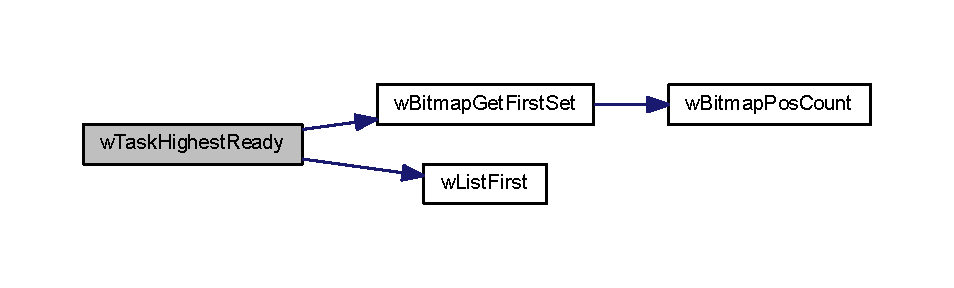
\includegraphics[width=350pt]{main_8c_aecc5337584ee14a8c816f9ce689ba128_cgraph}
\end{center}
\end{figure}
这是这个函数的调用关系图\+:
\nopagebreak
\begin{figure}[H]
\begin{center}
\leavevmode
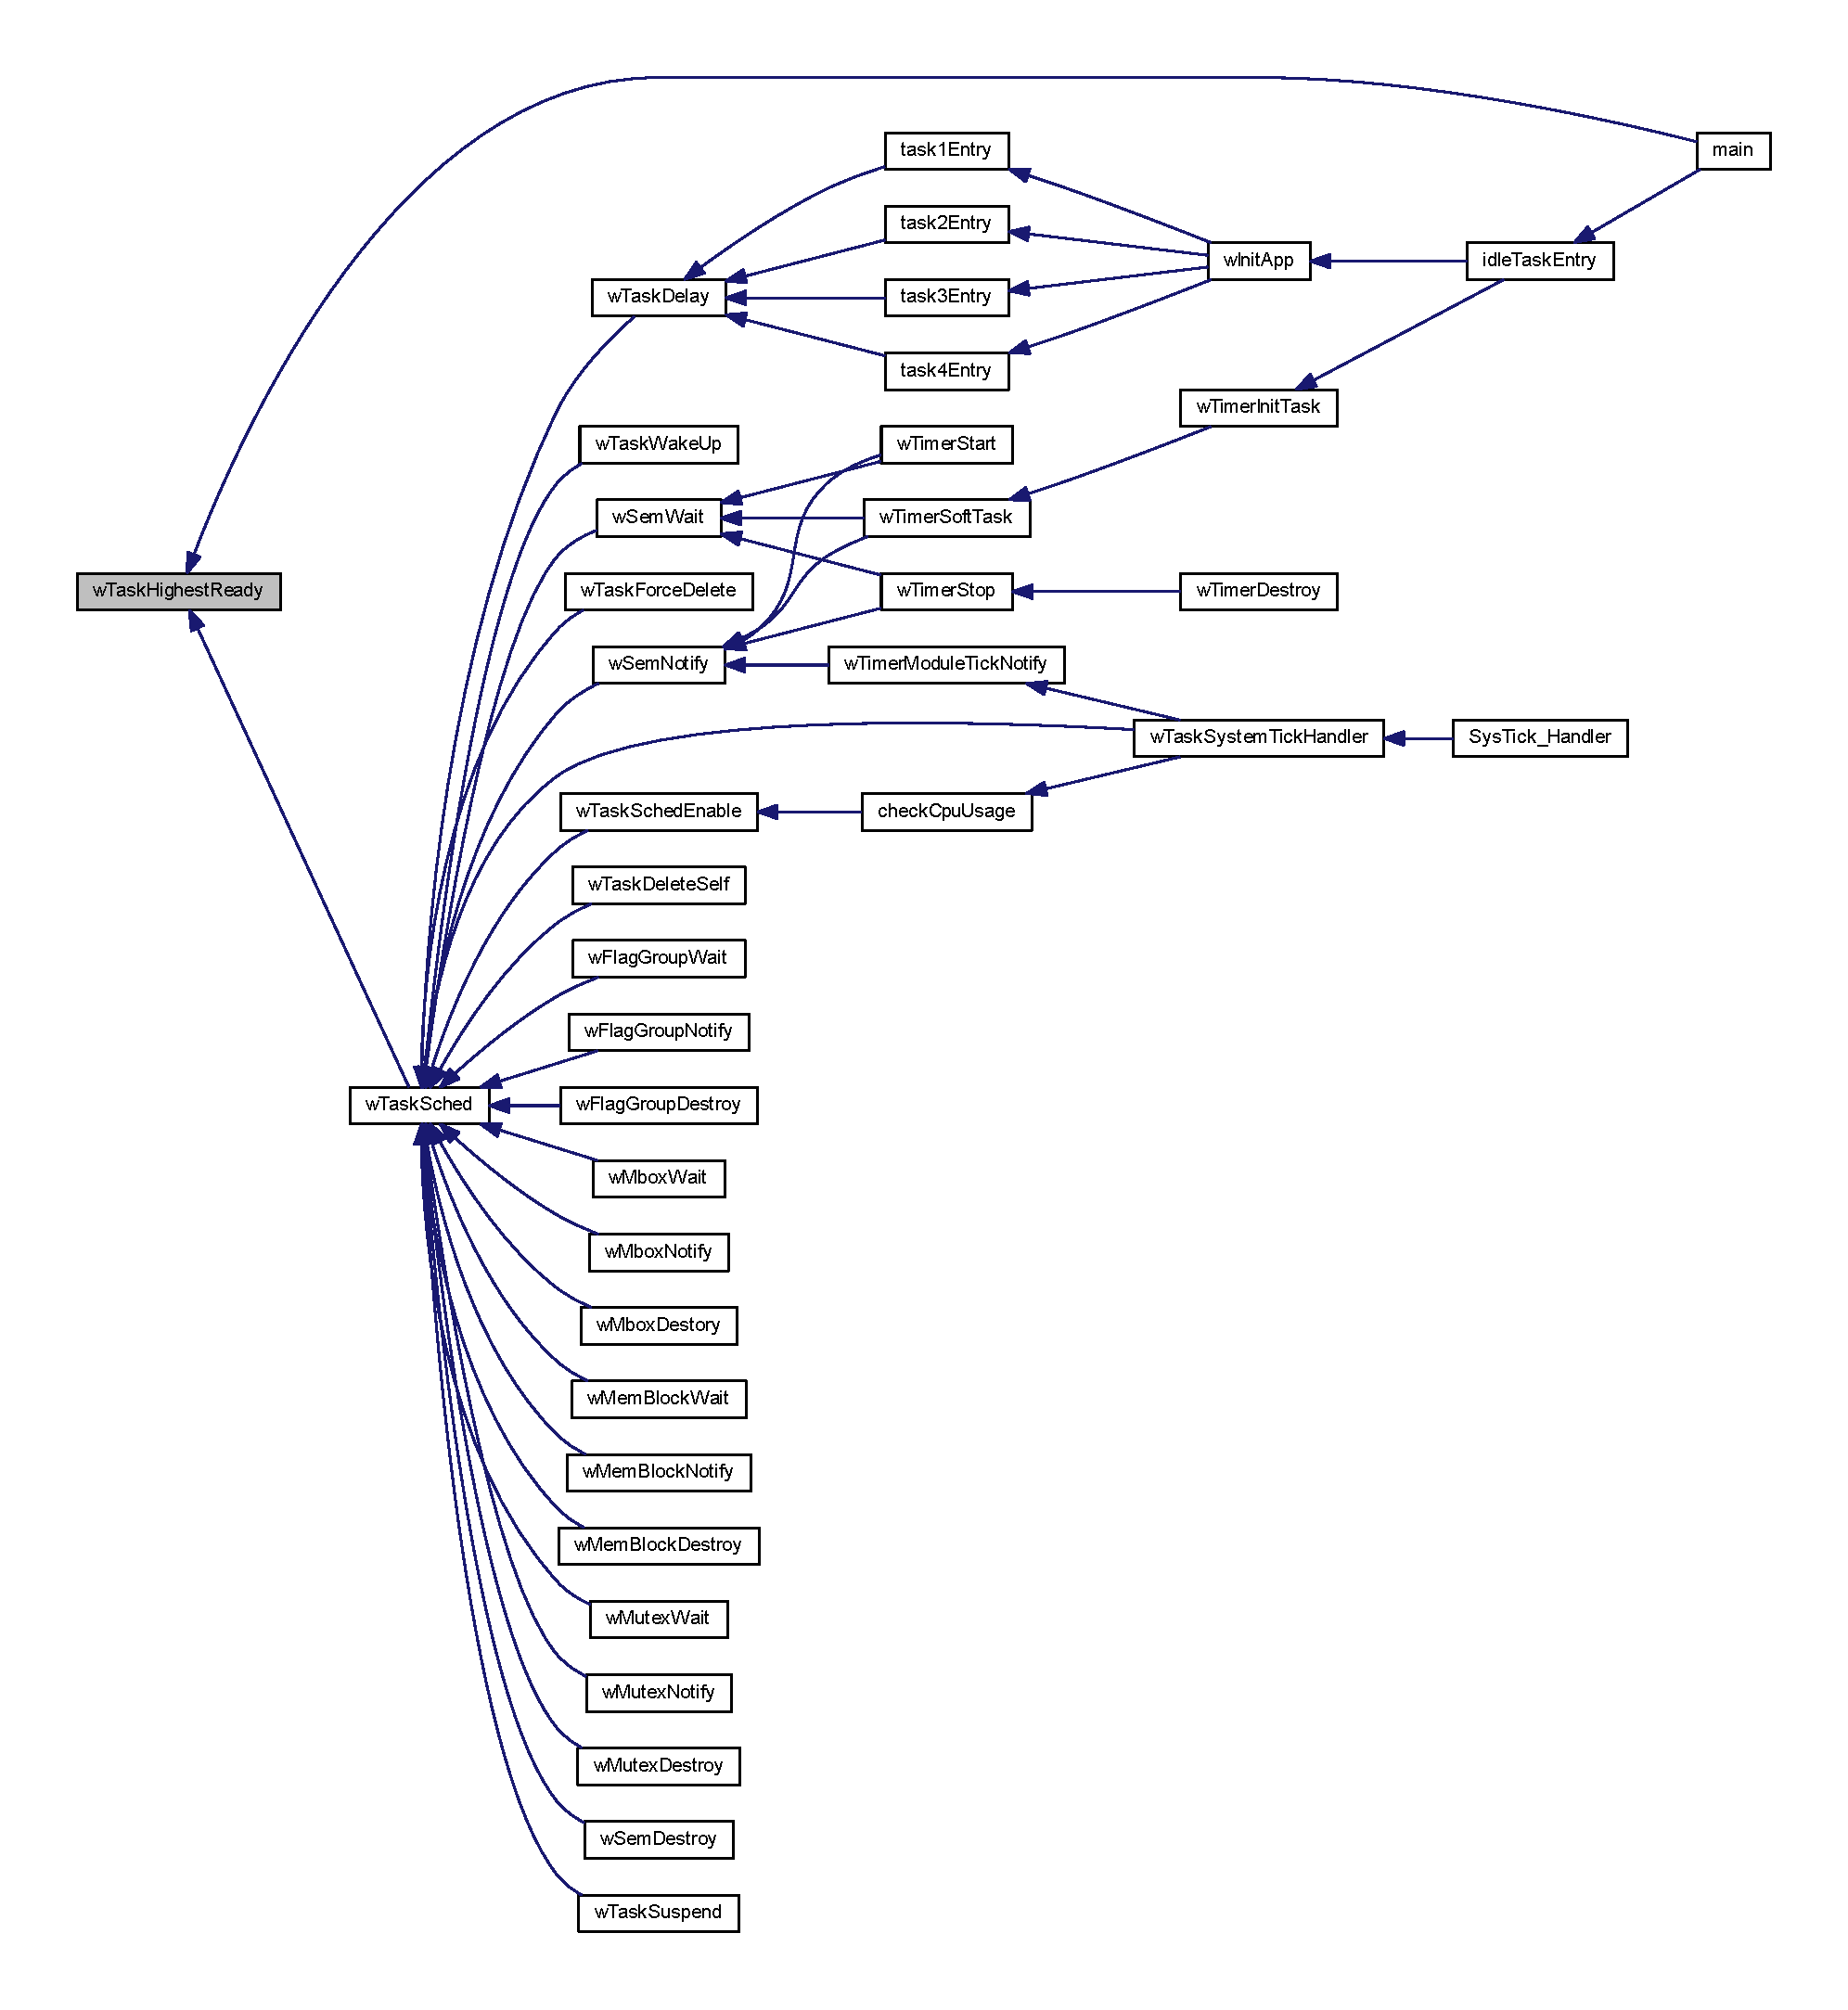
\includegraphics[width=350pt]{main_8c_aecc5337584ee14a8c816f9ce689ba128_icgraph}
\end{center}
\end{figure}
\mbox{\Hypertarget{main_8c_a231177ae77d1af6c5239c4ca95be8760}\label{main_8c_a231177ae77d1af6c5239c4ca95be8760}} 
\index{main.\+c@{main.\+c}!w\+Task\+Sched@{w\+Task\+Sched}}
\index{w\+Task\+Sched@{w\+Task\+Sched}!main.\+c@{main.\+c}}
\subsubsection{\texorpdfstring{w\+Task\+Sched()}{wTaskSched()}}
{\footnotesize\ttfamily void w\+Task\+Sched (\begin{DoxyParamCaption}\item[{void}]{ }\end{DoxyParamCaption})}



任务调度函数 


\begin{DoxyParams}{参数}
{\em 无} & \\
\hline
\end{DoxyParams}

\begin{DoxyRetVals}{返回值}
{\em 无} & \\
\hline
\end{DoxyRetVals}
函数调用图\+:
\nopagebreak
\begin{figure}[H]
\begin{center}
\leavevmode
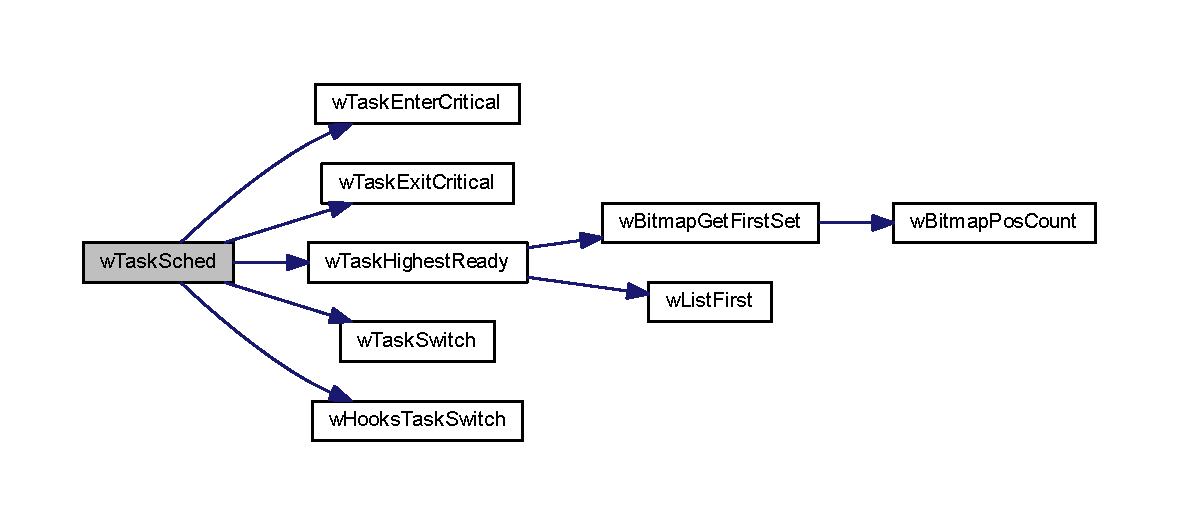
\includegraphics[width=350pt]{main_8c_a231177ae77d1af6c5239c4ca95be8760_cgraph}
\end{center}
\end{figure}
这是这个函数的调用关系图\+:
\nopagebreak
\begin{figure}[H]
\begin{center}
\leavevmode
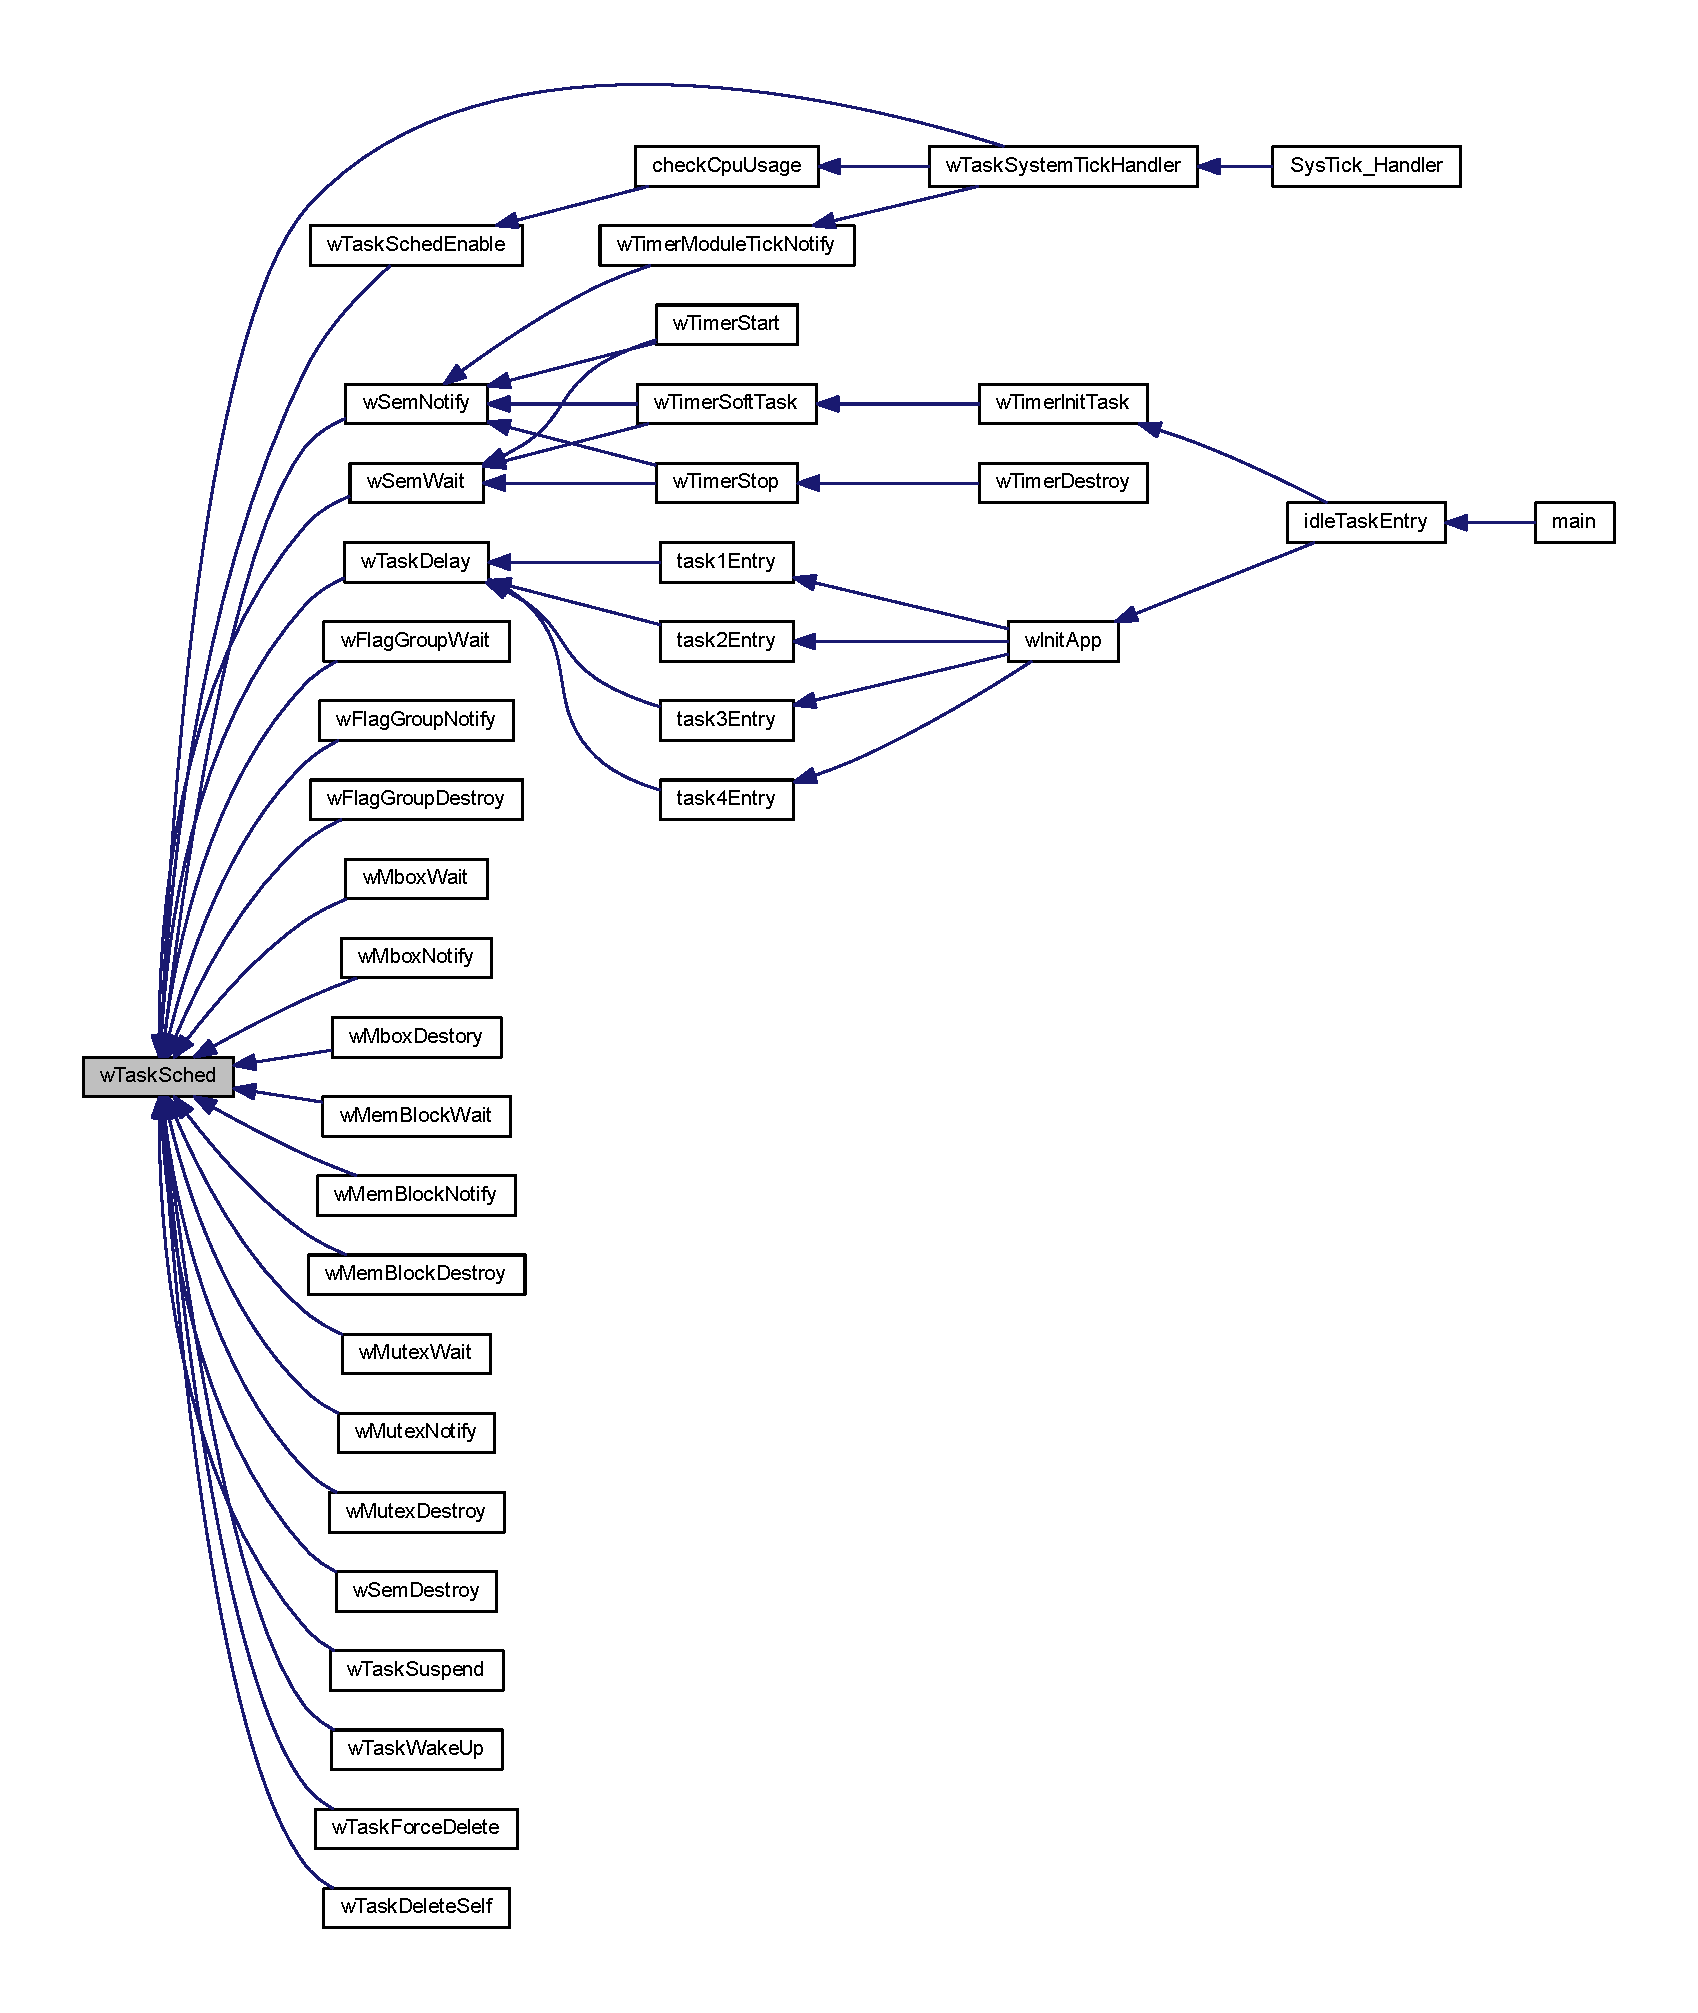
\includegraphics[width=350pt]{main_8c_a231177ae77d1af6c5239c4ca95be8760_icgraph}
\end{center}
\end{figure}
\mbox{\Hypertarget{main_8c_a033b0131d8e17bf2e857a743a02313f7}\label{main_8c_a033b0131d8e17bf2e857a743a02313f7}} 
\index{main.\+c@{main.\+c}!w\+Task\+Sched\+Disable@{w\+Task\+Sched\+Disable}}
\index{w\+Task\+Sched\+Disable@{w\+Task\+Sched\+Disable}!main.\+c@{main.\+c}}
\subsubsection{\texorpdfstring{w\+Task\+Sched\+Disable()}{wTaskSchedDisable()}}
{\footnotesize\ttfamily void w\+Task\+Sched\+Disable (\begin{DoxyParamCaption}\item[{void}]{ }\end{DoxyParamCaption})}



调度锁上锁函数 


\begin{DoxyParams}{参数}
{\em 无} & \\
\hline
\end{DoxyParams}

\begin{DoxyRetVals}{返回值}
{\em 无} & \\
\hline
\end{DoxyRetVals}
函数调用图\+:
\nopagebreak
\begin{figure}[H]
\begin{center}
\leavevmode
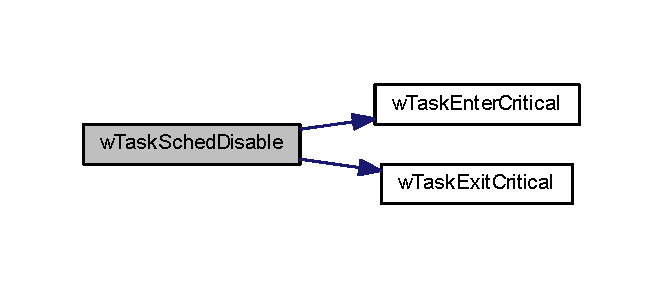
\includegraphics[width=318pt]{main_8c_a033b0131d8e17bf2e857a743a02313f7_cgraph}
\end{center}
\end{figure}
这是这个函数的调用关系图\+:
\nopagebreak
\begin{figure}[H]
\begin{center}
\leavevmode
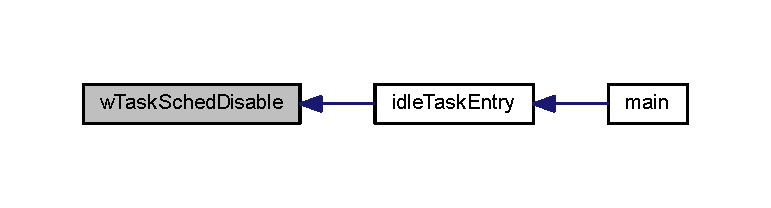
\includegraphics[width=350pt]{main_8c_a033b0131d8e17bf2e857a743a02313f7_icgraph}
\end{center}
\end{figure}
\mbox{\Hypertarget{main_8c_ae6dc919e0faa1e15e92c96899202c0a5}\label{main_8c_ae6dc919e0faa1e15e92c96899202c0a5}} 
\index{main.\+c@{main.\+c}!w\+Task\+Sched\+Enable@{w\+Task\+Sched\+Enable}}
\index{w\+Task\+Sched\+Enable@{w\+Task\+Sched\+Enable}!main.\+c@{main.\+c}}
\subsubsection{\texorpdfstring{w\+Task\+Sched\+Enable()}{wTaskSchedEnable()}}
{\footnotesize\ttfamily void w\+Task\+Sched\+Enable (\begin{DoxyParamCaption}\item[{void}]{ }\end{DoxyParamCaption})}



允许任务调度函数 


\begin{DoxyParams}{参数}
{\em 无} & \\
\hline
\end{DoxyParams}

\begin{DoxyRetVals}{返回值}
{\em 无} & \\
\hline
\end{DoxyRetVals}
函数调用图\+:
\nopagebreak
\begin{figure}[H]
\begin{center}
\leavevmode
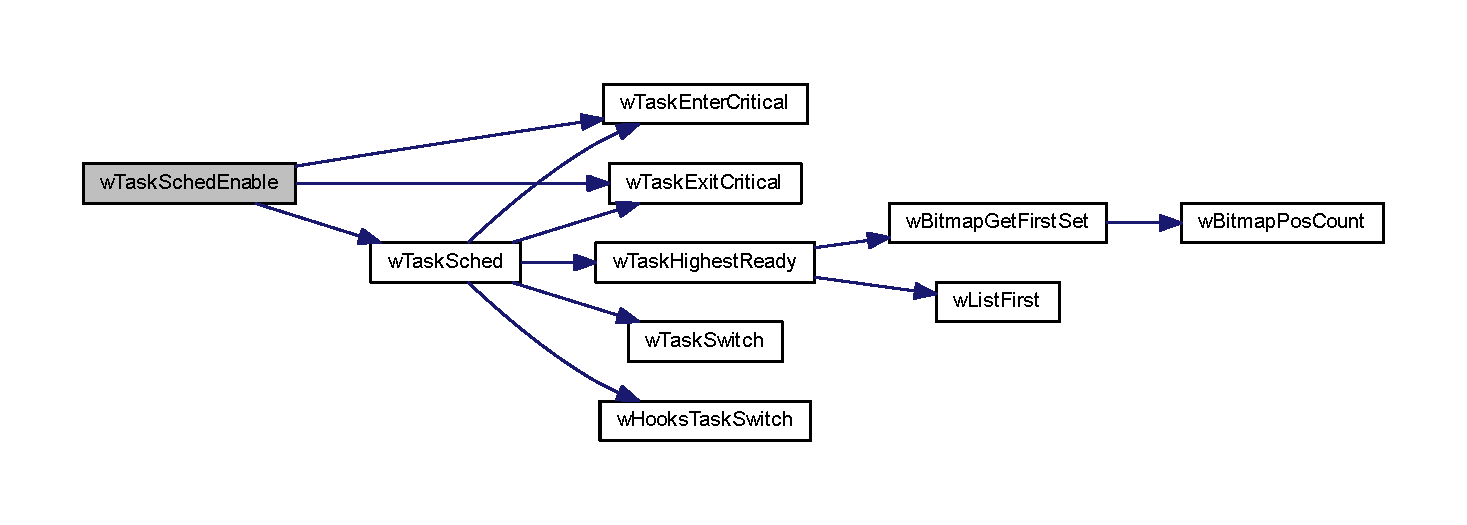
\includegraphics[width=350pt]{main_8c_ae6dc919e0faa1e15e92c96899202c0a5_cgraph}
\end{center}
\end{figure}
这是这个函数的调用关系图\+:
\nopagebreak
\begin{figure}[H]
\begin{center}
\leavevmode
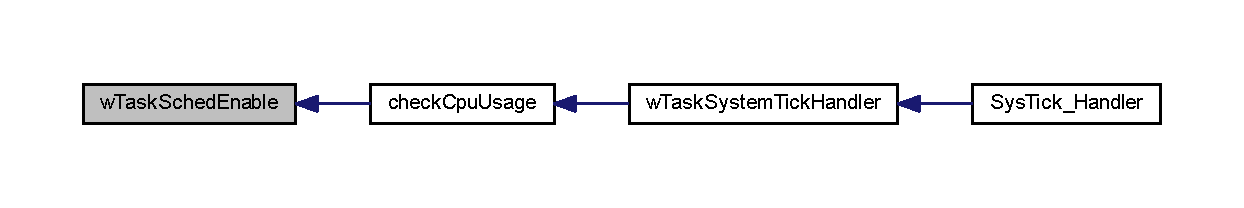
\includegraphics[width=350pt]{main_8c_ae6dc919e0faa1e15e92c96899202c0a5_icgraph}
\end{center}
\end{figure}
\mbox{\Hypertarget{main_8c_a4d9a0f3090b684084bbe94f148747cd0}\label{main_8c_a4d9a0f3090b684084bbe94f148747cd0}} 
\index{main.\+c@{main.\+c}!w\+Task\+Sched\+Init@{w\+Task\+Sched\+Init}}
\index{w\+Task\+Sched\+Init@{w\+Task\+Sched\+Init}!main.\+c@{main.\+c}}
\subsubsection{\texorpdfstring{w\+Task\+Sched\+Init()}{wTaskSchedInit()}}
{\footnotesize\ttfamily void w\+Task\+Sched\+Init (\begin{DoxyParamCaption}\item[{void}]{ }\end{DoxyParamCaption})}



内核初始化函数(初始化调度器) 


\begin{DoxyParams}{参数}
{\em 无} & \\
\hline
\end{DoxyParams}

\begin{DoxyRetVals}{返回值}
{\em 无} & \\
\hline
\end{DoxyRetVals}
函数调用图\+:
\nopagebreak
\begin{figure}[H]
\begin{center}
\leavevmode
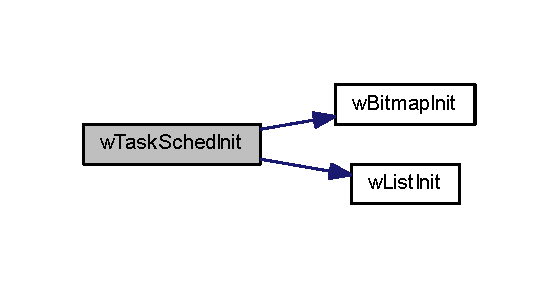
\includegraphics[width=268pt]{main_8c_a4d9a0f3090b684084bbe94f148747cd0_cgraph}
\end{center}
\end{figure}
这是这个函数的调用关系图\+:
\nopagebreak
\begin{figure}[H]
\begin{center}
\leavevmode
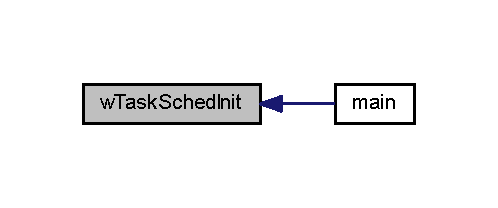
\includegraphics[width=239pt]{main_8c_a4d9a0f3090b684084bbe94f148747cd0_icgraph}
\end{center}
\end{figure}
\mbox{\Hypertarget{main_8c_a600f0ce279bbc48c121bd6e31874aff9}\label{main_8c_a600f0ce279bbc48c121bd6e31874aff9}} 
\index{main.\+c@{main.\+c}!w\+Task\+Sched\+Rdy@{w\+Task\+Sched\+Rdy}}
\index{w\+Task\+Sched\+Rdy@{w\+Task\+Sched\+Rdy}!main.\+c@{main.\+c}}
\subsubsection{\texorpdfstring{w\+Task\+Sched\+Rdy()}{wTaskSchedRdy()}}
{\footnotesize\ttfamily void w\+Task\+Sched\+Rdy (\begin{DoxyParamCaption}\item[{\mbox{\hyperlink{w_task_8h_acd0e6238476f631a6ac4588629bac372}{w\+Task}} $\ast$}]{task }\end{DoxyParamCaption})}



将任务插入就绪列表(将任务从延时队列中移除时)函数 


\begin{DoxyParams}{参数}
{\em task} & 任务结构指针 \\
\hline
\end{DoxyParams}

\begin{DoxyRetVals}{返回值}
{\em 无} & \\
\hline
\end{DoxyRetVals}
函数调用图\+:
\nopagebreak
\begin{figure}[H]
\begin{center}
\leavevmode
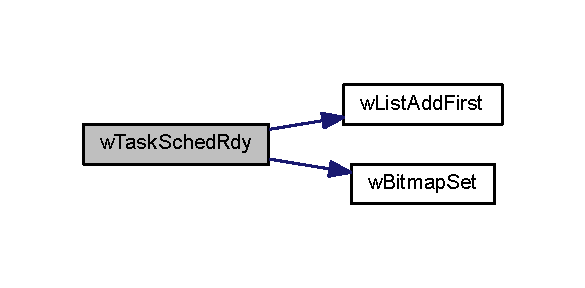
\includegraphics[width=281pt]{main_8c_a600f0ce279bbc48c121bd6e31874aff9_cgraph}
\end{center}
\end{figure}
这是这个函数的调用关系图\+:
\nopagebreak
\begin{figure}[H]
\begin{center}
\leavevmode
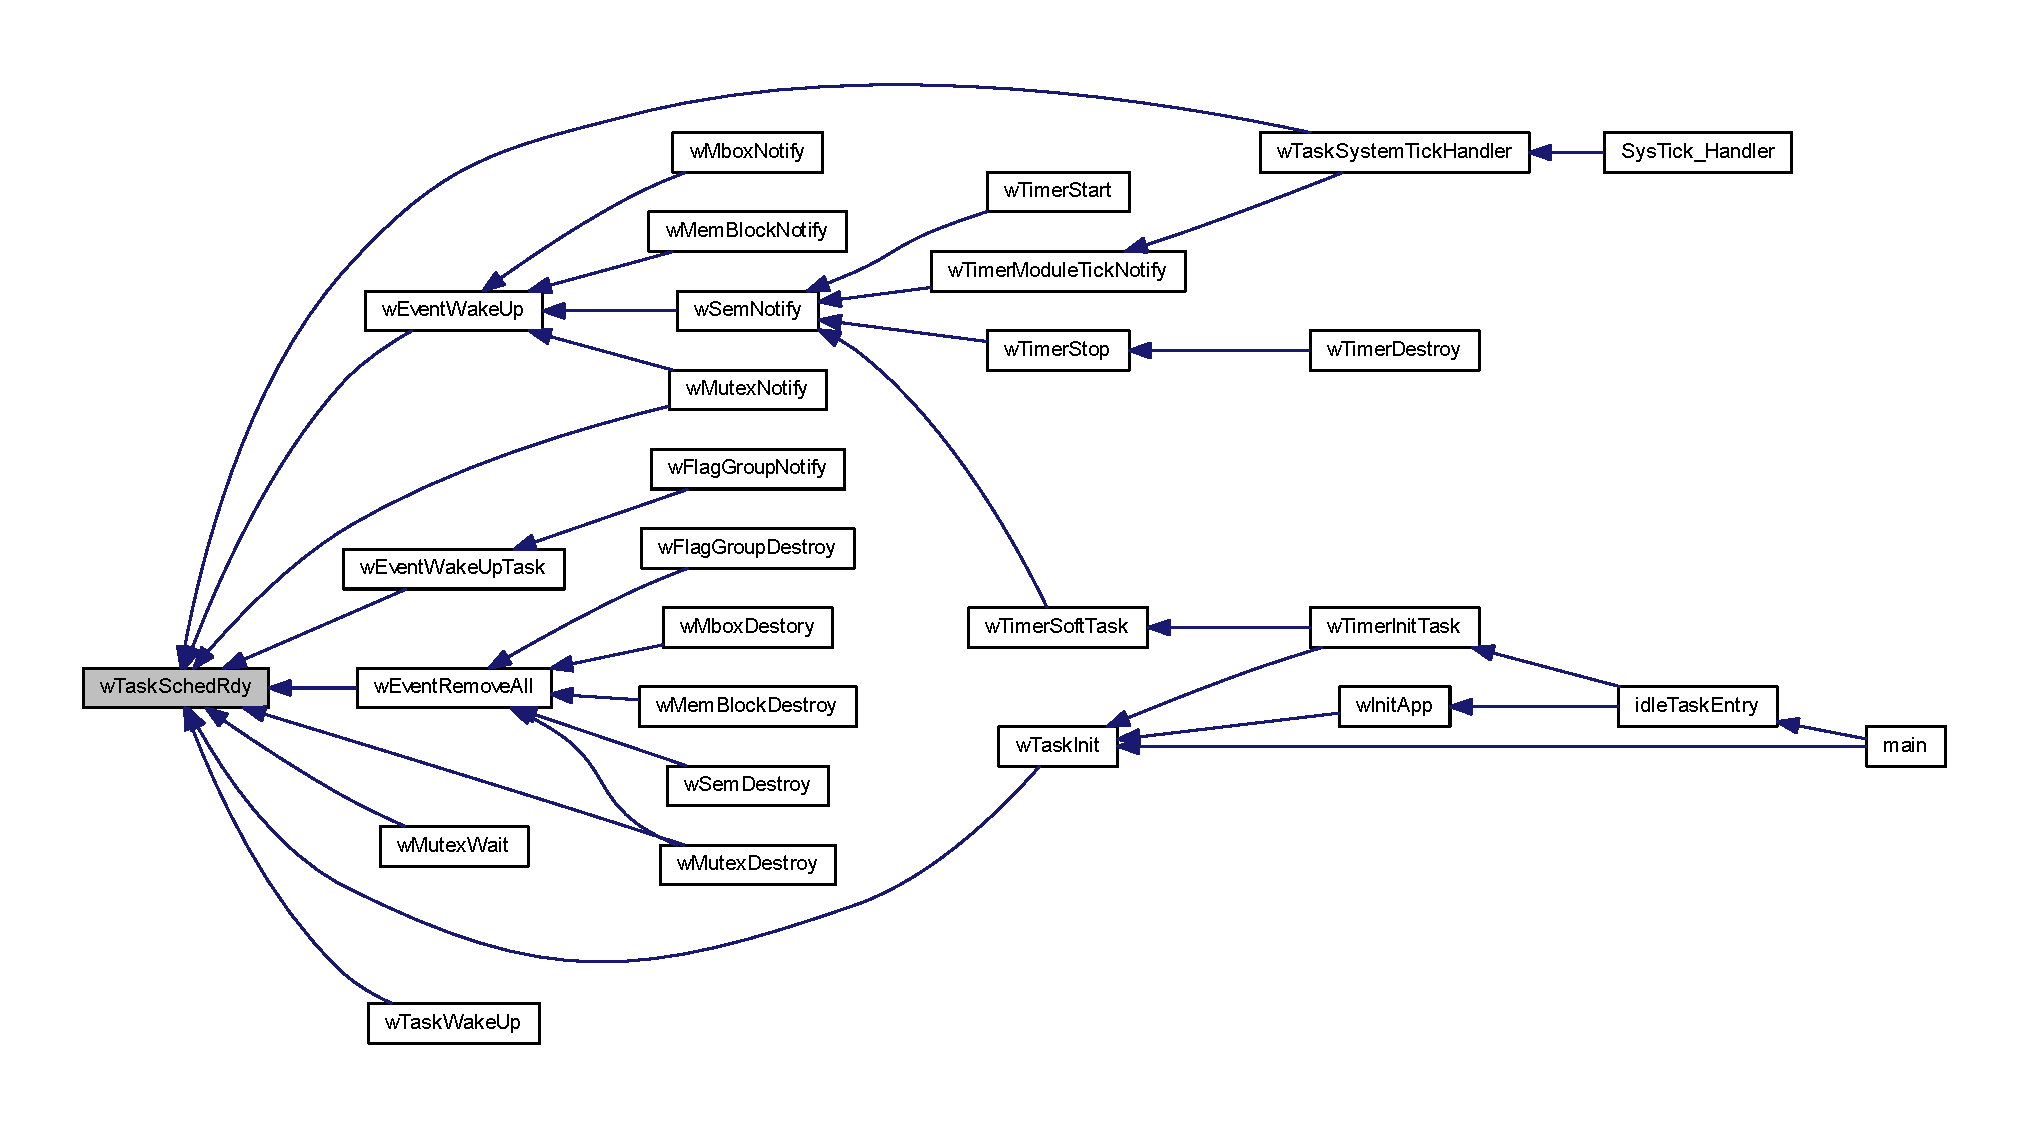
\includegraphics[width=350pt]{main_8c_a600f0ce279bbc48c121bd6e31874aff9_icgraph}
\end{center}
\end{figure}
\mbox{\Hypertarget{main_8c_ad212054b17e4733e330c97f3d3274767}\label{main_8c_ad212054b17e4733e330c97f3d3274767}} 
\index{main.\+c@{main.\+c}!w\+Task\+Sched\+Remove@{w\+Task\+Sched\+Remove}}
\index{w\+Task\+Sched\+Remove@{w\+Task\+Sched\+Remove}!main.\+c@{main.\+c}}
\subsubsection{\texorpdfstring{w\+Task\+Sched\+Remove()}{wTaskSchedRemove()}}
{\footnotesize\ttfamily void w\+Task\+Sched\+Remove (\begin{DoxyParamCaption}\item[{\mbox{\hyperlink{w_task_8h_acd0e6238476f631a6ac4588629bac372}{w\+Task}} $\ast$}]{task }\end{DoxyParamCaption})}



将任务从优先级列表中删除函数 


\begin{DoxyParams}{参数}
{\em task} & 任务结构指针 \\
\hline
\end{DoxyParams}

\begin{DoxyRetVals}{返回值}
{\em 无} & \\
\hline
\end{DoxyRetVals}
函数调用图\+:
\nopagebreak
\begin{figure}[H]
\begin{center}
\leavevmode
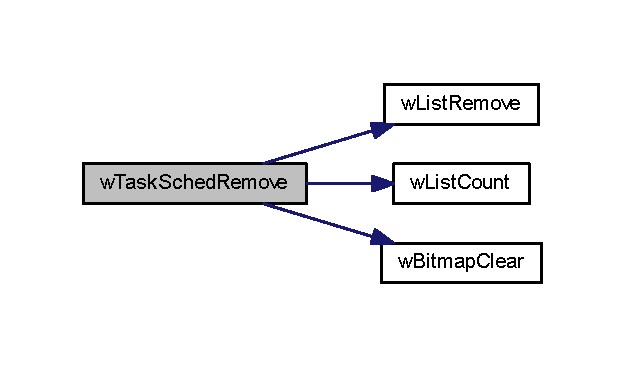
\includegraphics[width=300pt]{main_8c_ad212054b17e4733e330c97f3d3274767_cgraph}
\end{center}
\end{figure}
这是这个函数的调用关系图\+:
\nopagebreak
\begin{figure}[H]
\begin{center}
\leavevmode
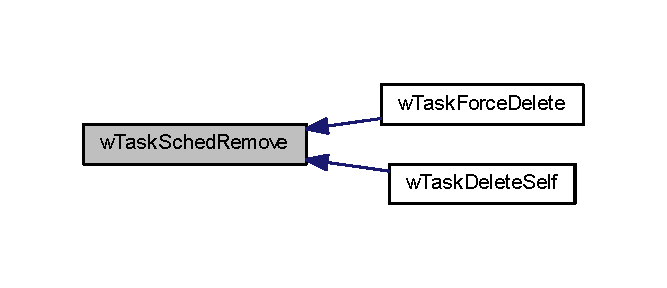
\includegraphics[width=320pt]{main_8c_ad212054b17e4733e330c97f3d3274767_icgraph}
\end{center}
\end{figure}
\mbox{\Hypertarget{main_8c_a598536b78a16c960ddfb82d887746cae}\label{main_8c_a598536b78a16c960ddfb82d887746cae}} 
\index{main.\+c@{main.\+c}!w\+Task\+Sched\+Un\+Rdy@{w\+Task\+Sched\+Un\+Rdy}}
\index{w\+Task\+Sched\+Un\+Rdy@{w\+Task\+Sched\+Un\+Rdy}!main.\+c@{main.\+c}}
\subsubsection{\texorpdfstring{w\+Task\+Sched\+Un\+Rdy()}{wTaskSchedUnRdy()}}
{\footnotesize\ttfamily void w\+Task\+Sched\+Un\+Rdy (\begin{DoxyParamCaption}\item[{\mbox{\hyperlink{w_task_8h_acd0e6238476f631a6ac4588629bac372}{w\+Task}} $\ast$}]{task }\end{DoxyParamCaption})}



将任务从就绪列表中删除函数 


\begin{DoxyParams}{参数}
{\em task} & 任务结构指针 \\
\hline
\end{DoxyParams}

\begin{DoxyRetVals}{返回值}
{\em 无} & \\
\hline
\end{DoxyRetVals}
函数调用图\+:
\nopagebreak
\begin{figure}[H]
\begin{center}
\leavevmode
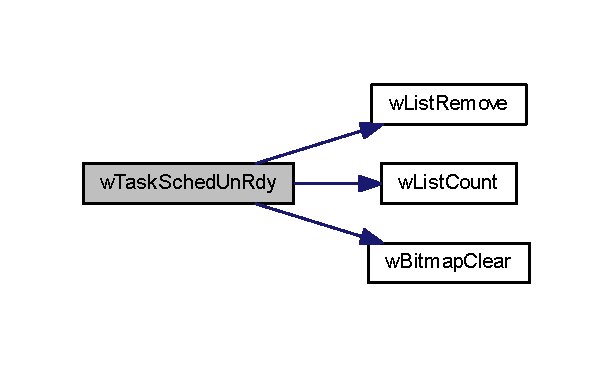
\includegraphics[width=294pt]{main_8c_a598536b78a16c960ddfb82d887746cae_cgraph}
\end{center}
\end{figure}
这是这个函数的调用关系图\+:
\nopagebreak
\begin{figure}[H]
\begin{center}
\leavevmode
\includegraphics[width=350pt]{main_8c_a598536b78a16c960ddfb82d887746cae_icgraph}
\end{center}
\end{figure}
\mbox{\Hypertarget{main_8c_a36ab31adb9bd20b1fe3337cf8ac6baf2}\label{main_8c_a36ab31adb9bd20b1fe3337cf8ac6baf2}} 
\index{main.\+c@{main.\+c}!w\+Task\+System\+Tick\+Handler@{w\+Task\+System\+Tick\+Handler}}
\index{w\+Task\+System\+Tick\+Handler@{w\+Task\+System\+Tick\+Handler}!main.\+c@{main.\+c}}
\subsubsection{\texorpdfstring{w\+Task\+System\+Tick\+Handler()}{wTaskSystemTickHandler()}}
{\footnotesize\ttfamily void w\+Task\+System\+Tick\+Handler (\begin{DoxyParamCaption}\item[{void}]{ }\end{DoxyParamCaption})}



任务\+System\+Tick中断服务函数 


\begin{DoxyParams}{参数}
{\em 无} & \\
\hline
\end{DoxyParams}

\begin{DoxyRetVals}{返回值}
{\em 无} & \\
\hline
\end{DoxyRetVals}
函数调用图\+:
\nopagebreak
\begin{figure}[H]
\begin{center}
\leavevmode
\includegraphics[width=350pt]{main_8c_a36ab31adb9bd20b1fe3337cf8ac6baf2_cgraph}
\end{center}
\end{figure}
这是这个函数的调用关系图\+:
\nopagebreak
\begin{figure}[H]
\begin{center}
\leavevmode
\includegraphics[width=335pt]{main_8c_a36ab31adb9bd20b1fe3337cf8ac6baf2_icgraph}
\end{center}
\end{figure}
\mbox{\Hypertarget{main_8c_a135f5a694c1f6b01cb1499ecaf2ee0a5}\label{main_8c_a135f5a694c1f6b01cb1499ecaf2ee0a5}} 
\index{main.\+c@{main.\+c}!w\+Time\+Task\+Remove@{w\+Time\+Task\+Remove}}
\index{w\+Time\+Task\+Remove@{w\+Time\+Task\+Remove}!main.\+c@{main.\+c}}
\subsubsection{\texorpdfstring{w\+Time\+Task\+Remove()}{wTimeTaskRemove()}}
{\footnotesize\ttfamily void w\+Time\+Task\+Remove (\begin{DoxyParamCaption}\item[{\mbox{\hyperlink{w_task_8h_acd0e6238476f631a6ac4588629bac372}{w\+Task}} $\ast$}]{task }\end{DoxyParamCaption})}



将任务从延时队列删除函数 


\begin{DoxyParams}{参数}
{\em task} & 延时结构指针 \\
\hline
\end{DoxyParams}

\begin{DoxyRetVals}{返回值}
{\em 无} & \\
\hline
\end{DoxyRetVals}
函数调用图\+:
\nopagebreak
\begin{figure}[H]
\begin{center}
\leavevmode
\includegraphics[width=290pt]{main_8c_a135f5a694c1f6b01cb1499ecaf2ee0a5_cgraph}
\end{center}
\end{figure}
这是这个函数的调用关系图\+:
\nopagebreak
\begin{figure}[H]
\begin{center}
\leavevmode
\includegraphics[width=313pt]{main_8c_a135f5a694c1f6b01cb1499ecaf2ee0a5_icgraph}
\end{center}
\end{figure}
\mbox{\Hypertarget{main_8c_a1163983eff6acb009950c69f3a55b629}\label{main_8c_a1163983eff6acb009950c69f3a55b629}} 
\index{main.\+c@{main.\+c}!w\+Time\+Task\+Wait@{w\+Time\+Task\+Wait}}
\index{w\+Time\+Task\+Wait@{w\+Time\+Task\+Wait}!main.\+c@{main.\+c}}
\subsubsection{\texorpdfstring{w\+Time\+Task\+Wait()}{wTimeTaskWait()}}
{\footnotesize\ttfamily void w\+Time\+Task\+Wait (\begin{DoxyParamCaption}\item[{\mbox{\hyperlink{w_task_8h_acd0e6238476f631a6ac4588629bac372}{w\+Task}} $\ast$}]{task,  }\item[{uint32\+\_\+t}]{ticks }\end{DoxyParamCaption})}



将任务插入延时队列函数 


\begin{DoxyParams}{参数}
{\em task} & 任务结构指针 \\
\hline
{\em ticks} & 延时的ticks数 \\
\hline
\end{DoxyParams}

\begin{DoxyRetVals}{返回值}
{\em 无} & \\
\hline
\end{DoxyRetVals}
函数调用图\+:
\nopagebreak
\begin{figure}[H]
\begin{center}
\leavevmode
\includegraphics[width=277pt]{main_8c_a1163983eff6acb009950c69f3a55b629_cgraph}
\end{center}
\end{figure}
这是这个函数的调用关系图\+:
\nopagebreak
\begin{figure}[H]
\begin{center}
\leavevmode
\includegraphics[width=350pt]{main_8c_a1163983eff6acb009950c69f3a55b629_icgraph}
\end{center}
\end{figure}
\mbox{\Hypertarget{main_8c_a85848b63b5fe499d55e6c4196c43f306}\label{main_8c_a85848b63b5fe499d55e6c4196c43f306}} 
\index{main.\+c@{main.\+c}!w\+Time\+Task\+Wake\+Up@{w\+Time\+Task\+Wake\+Up}}
\index{w\+Time\+Task\+Wake\+Up@{w\+Time\+Task\+Wake\+Up}!main.\+c@{main.\+c}}
\subsubsection{\texorpdfstring{w\+Time\+Task\+Wake\+Up()}{wTimeTaskWakeUp()}}
{\footnotesize\ttfamily void w\+Time\+Task\+Wake\+Up (\begin{DoxyParamCaption}\item[{\mbox{\hyperlink{w_task_8h_acd0e6238476f631a6ac4588629bac372}{w\+Task}} $\ast$}]{task }\end{DoxyParamCaption})}



将任务从延时队列唤醒函数 


\begin{DoxyParams}{参数}
{\em task} & 延时结构指针 \\
\hline
\end{DoxyParams}

\begin{DoxyRetVals}{返回值}
{\em 无} & \\
\hline
\end{DoxyRetVals}
函数调用图\+:
\nopagebreak
\begin{figure}[H]
\begin{center}
\leavevmode
\includegraphics[width=293pt]{main_8c_a85848b63b5fe499d55e6c4196c43f306_cgraph}
\end{center}
\end{figure}
这是这个函数的调用关系图\+:
\nopagebreak
\begin{figure}[H]
\begin{center}
\leavevmode
\includegraphics[width=350pt]{main_8c_a85848b63b5fe499d55e6c4196c43f306_icgraph}
\end{center}
\end{figure}
\mbox{\Hypertarget{main_8c_ad2cede6eea6a293ae82a1cedb76bc6f3}\label{main_8c_ad2cede6eea6a293ae82a1cedb76bc6f3}} 
\index{main.\+c@{main.\+c}!w\+Time\+Tick\+Init@{w\+Time\+Tick\+Init}}
\index{w\+Time\+Tick\+Init@{w\+Time\+Tick\+Init}!main.\+c@{main.\+c}}
\subsubsection{\texorpdfstring{w\+Time\+Tick\+Init()}{wTimeTickInit()}}
{\footnotesize\ttfamily void w\+Time\+Tick\+Init (\begin{DoxyParamCaption}\item[{void}]{ }\end{DoxyParamCaption})}



时钟节拍计数器初始化函数 


\begin{DoxyParams}{参数}
{\em 无} & \\
\hline
\end{DoxyParams}

\begin{DoxyRetVals}{返回值}
{\em 无} & \\
\hline
\end{DoxyRetVals}
这是这个函数的调用关系图\+:
\nopagebreak
\begin{figure}[H]
\begin{center}
\leavevmode
\includegraphics[width=229pt]{main_8c_ad2cede6eea6a293ae82a1cedb76bc6f3_icgraph}
\end{center}
\end{figure}


\subsection{变量说明}
\mbox{\Hypertarget{main_8c_a4d3fcca6f9564b4467b34cfa39cd5310}\label{main_8c_a4d3fcca6f9564b4467b34cfa39cd5310}} 
\index{main.\+c@{main.\+c}!cpu\+Usage@{cpu\+Usage}}
\index{cpu\+Usage@{cpu\+Usage}!main.\+c@{main.\+c}}
\subsubsection{\texorpdfstring{cpu\+Usage}{cpuUsage}}
{\footnotesize\ttfamily float cpu\+Usage\hspace{0.3cm}{\ttfamily [static]}}

cpu使用率统计 \mbox{\Hypertarget{main_8c_a6bec055003640755e2481f3cf0692894}\label{main_8c_a6bec055003640755e2481f3cf0692894}} 
\index{main.\+c@{main.\+c}!current\+Task@{current\+Task}}
\index{current\+Task@{current\+Task}!main.\+c@{main.\+c}}
\subsubsection{\texorpdfstring{current\+Task}{currentTask}}
{\footnotesize\ttfamily \mbox{\hyperlink{w_task_8h_acd0e6238476f631a6ac4588629bac372}{w\+Task}}$\ast$ current\+Task}

指向当前任务的指针 \mbox{\Hypertarget{main_8c_ae640b280f11b1ff0b28135982bbac7f5}\label{main_8c_ae640b280f11b1ff0b28135982bbac7f5}} 
\index{main.\+c@{main.\+c}!enable\+Cpu\+Usage\+Stat@{enable\+Cpu\+Usage\+Stat}}
\index{enable\+Cpu\+Usage\+Stat@{enable\+Cpu\+Usage\+Stat}!main.\+c@{main.\+c}}
\subsubsection{\texorpdfstring{enable\+Cpu\+Usage\+Stat}{enableCpuUsageStat}}
{\footnotesize\ttfamily uint32\+\_\+t enable\+Cpu\+Usage\+Stat\hspace{0.3cm}{\ttfamily [static]}}

是否使能cpu统计 \mbox{\Hypertarget{main_8c_a9979e3c27f522bb6d13cff22efd2e488}\label{main_8c_a9979e3c27f522bb6d13cff22efd2e488}} 
\index{main.\+c@{main.\+c}!idle\+Count@{idle\+Count}}
\index{idle\+Count@{idle\+Count}!main.\+c@{main.\+c}}
\subsubsection{\texorpdfstring{idle\+Count}{idleCount}}
{\footnotesize\ttfamily uint32\+\_\+t idle\+Count}

空闲任务计数器 \mbox{\Hypertarget{main_8c_aba65b5ed5e394f5ca1f346b4a53364cf}\label{main_8c_aba65b5ed5e394f5ca1f346b4a53364cf}} 
\index{main.\+c@{main.\+c}!idle\+Max\+Count@{idle\+Max\+Count}}
\index{idle\+Max\+Count@{idle\+Max\+Count}!main.\+c@{main.\+c}}
\subsubsection{\texorpdfstring{idle\+Max\+Count}{idleMaxCount}}
{\footnotesize\ttfamily uint32\+\_\+t idle\+Max\+Count}

空闲任务最大计数器 \mbox{\Hypertarget{main_8c_a23c0ee4b0c015f3388e9e2dde31c66bb}\label{main_8c_a23c0ee4b0c015f3388e9e2dde31c66bb}} 
\index{main.\+c@{main.\+c}!idle\+Task@{idle\+Task}}
\index{idle\+Task@{idle\+Task}!main.\+c@{main.\+c}}
\subsubsection{\texorpdfstring{idle\+Task}{idleTask}}
{\footnotesize\ttfamily \mbox{\hyperlink{w_task_8h_acd0e6238476f631a6ac4588629bac372}{w\+Task}}$\ast$ idle\+Task}

指向空闲任务的指针 \mbox{\Hypertarget{main_8c_ad6edc236a894fc8b921be2739d43ff24}\label{main_8c_ad6edc236a894fc8b921be2739d43ff24}} 
\index{main.\+c@{main.\+c}!idle\+Task\+Env@{idle\+Task\+Env}}
\index{idle\+Task\+Env@{idle\+Task\+Env}!main.\+c@{main.\+c}}
\subsubsection{\texorpdfstring{idle\+Task\+Env}{idleTaskEnv}}
{\footnotesize\ttfamily \mbox{\hyperlink{w_task_8h_ae1dd34929f40dd21d0ea81f2d3f1c2e0}{w\+Task\+Stack}} idle\+Task\+Env\mbox{[}\mbox{\hyperlink{w_config_8h_a9991397c90242f684eb25692adbfdc77}{W\+Q\+\_\+\+O\+S\+\_\+\+I\+D\+L\+E\+T\+A\+S\+K\+\_\+\+S\+T\+A\+C\+K\+\_\+\+S\+I\+ZE}}\mbox{]}}

\mbox{\Hypertarget{main_8c_a44a5b29a47ca1930c940bc88c9051e0e}\label{main_8c_a44a5b29a47ca1930c940bc88c9051e0e}} 
\index{main.\+c@{main.\+c}!next\+Task@{next\+Task}}
\index{next\+Task@{next\+Task}!main.\+c@{main.\+c}}
\subsubsection{\texorpdfstring{next\+Task}{nextTask}}
{\footnotesize\ttfamily \mbox{\hyperlink{w_task_8h_acd0e6238476f631a6ac4588629bac372}{w\+Task}}$\ast$ next\+Task}

指向将要运行任务的指针 \mbox{\Hypertarget{main_8c_a9fcac63fa1ff9049d9b30424558b1d30}\label{main_8c_a9fcac63fa1ff9049d9b30424558b1d30}} 
\index{main.\+c@{main.\+c}!schedlock\+Count@{schedlock\+Count}}
\index{schedlock\+Count@{schedlock\+Count}!main.\+c@{main.\+c}}
\subsubsection{\texorpdfstring{schedlock\+Count}{schedlockCount}}
{\footnotesize\ttfamily uint8\+\_\+t schedlock\+Count}

调度锁计数器 \mbox{\Hypertarget{main_8c_a59fae34e401c2e655eee7ffc8981189f}\label{main_8c_a59fae34e401c2e655eee7ffc8981189f}} 
\index{main.\+c@{main.\+c}!task\+Prio\+Bitmap@{task\+Prio\+Bitmap}}
\index{task\+Prio\+Bitmap@{task\+Prio\+Bitmap}!main.\+c@{main.\+c}}
\subsubsection{\texorpdfstring{task\+Prio\+Bitmap}{taskPrioBitmap}}
{\footnotesize\ttfamily \mbox{\hyperlink{structw_bitmap}{w\+Bitmap}} task\+Prio\+Bitmap}

任务优先级位图 \mbox{\Hypertarget{main_8c_aad68ddf20dbfe94a640011019f2e2bbc}\label{main_8c_aad68ddf20dbfe94a640011019f2e2bbc}} 
\index{main.\+c@{main.\+c}!task\+Table@{task\+Table}}
\index{task\+Table@{task\+Table}!main.\+c@{main.\+c}}
\subsubsection{\texorpdfstring{task\+Table}{taskTable}}
{\footnotesize\ttfamily \mbox{\hyperlink{w_lib_8h_a3f922f977222a1e1fc18bd2ce6d668c3}{w\+List}} task\+Table\mbox{[}\mbox{\hyperlink{w_config_8h_ac74e7af2bb0660ccb34d04ef1e5a48d2}{W\+Q\+\_\+\+O\+S\+\_\+\+P\+R\+O\+\_\+\+C\+O\+U\+NT}}\mbox{]}}

任务就绪表 \mbox{\Hypertarget{main_8c_af4fc7964f7a64a2a55f189f4533015f4}\label{main_8c_af4fc7964f7a64a2a55f189f4533015f4}} 
\index{main.\+c@{main.\+c}!tick\+Count@{tick\+Count}}
\index{tick\+Count@{tick\+Count}!main.\+c@{main.\+c}}
\subsubsection{\texorpdfstring{tick\+Count}{tickCount}}
{\footnotesize\ttfamily uint32\+\_\+t tick\+Count}

时钟节拍计数器 \mbox{\Hypertarget{main_8c_a5fb74394eca3c48232b60346daa851b7}\label{main_8c_a5fb74394eca3c48232b60346daa851b7}} 
\index{main.\+c@{main.\+c}!w\+Task\+Delay\+List@{w\+Task\+Delay\+List}}
\index{w\+Task\+Delay\+List@{w\+Task\+Delay\+List}!main.\+c@{main.\+c}}
\subsubsection{\texorpdfstring{w\+Task\+Delay\+List}{wTaskDelayList}}
{\footnotesize\ttfamily \mbox{\hyperlink{w_lib_8h_a3f922f977222a1e1fc18bd2ce6d668c3}{w\+List}} w\+Task\+Delay\+List}

延时队列 \mbox{\Hypertarget{main_8c_aa6ce5811e5fc82d1c0b0c9526e3ee2dc}\label{main_8c_aa6ce5811e5fc82d1c0b0c9526e3ee2dc}} 
\index{main.\+c@{main.\+c}!w\+Task\+Idle@{w\+Task\+Idle}}
\index{w\+Task\+Idle@{w\+Task\+Idle}!main.\+c@{main.\+c}}
\subsubsection{\texorpdfstring{w\+Task\+Idle}{wTaskIdle}}
{\footnotesize\ttfamily \mbox{\hyperlink{w_task_8h_acd0e6238476f631a6ac4588629bac372}{w\+Task}} w\+Task\+Idle}


\hypertarget{switch_8c}{}\section{C\+:/\+Users/pc/\+Desktop/\+W\+Q\+\_\+\+O\+S/\+Project/\+Sourse/switch.c 文件参考}
\label{switch_8c}\index{C\+:/\+Users/pc/\+Desktop/\+W\+Q\+\_\+\+O\+S/\+Project/\+Sourse/switch.\+c@{C\+:/\+Users/pc/\+Desktop/\+W\+Q\+\_\+\+O\+S/\+Project/\+Sourse/switch.\+c}}
{\ttfamily \#include \char`\"{}W\+Q\+\_\+\+O\+S.\+h\char`\"{}}\newline
{\ttfamily \#include \char`\"{}A\+R\+M\+C\+M3.\+h\char`\"{}}\newline
switch.\+c 的引用(Include)关系图\+:
\nopagebreak
\begin{figure}[H]
\begin{center}
\leavevmode
\includegraphics[width=350pt]{switch_8c__incl}
\end{center}
\end{figure}
\subsection*{宏定义}
\begin{DoxyCompactItemize}
\item 
\#define \mbox{\hyperlink{switch_8c_afa1ca44ad548bf5bfa2f19d7438c722a}{N\+V\+I\+C\+\_\+\+I\+N\+T\+\_\+\+C\+T\+RL}}~0x\+E000\+E\+D04
\item 
\#define \mbox{\hyperlink{switch_8c_a11166a59c430ba34e6da8e20571b58d7}{N\+V\+I\+C\+\_\+\+P\+E\+N\+D\+S\+V\+S\+ET}}~0x10000000
\item 
\#define \mbox{\hyperlink{switch_8c_a23694ffa1ac38dfdfcc1ae1160be7397}{N\+V\+I\+C\+\_\+\+S\+Y\+S\+P\+R\+I2}}~0x\+E000\+E\+D22
\item 
\#define \mbox{\hyperlink{switch_8c_a39caf8bb045502e6f5611403dc4d121d}{N\+V\+I\+C\+\_\+\+P\+E\+N\+D\+S\+V\+\_\+\+P\+RT}}~0x000000\+FF
\item 
\#define \mbox{\hyperlink{switch_8c_ade1e623e8a7851917439eeac2019ff3f}{M\+E\+M32}}(addr)~$\ast$(volatile unsigned long $\ast$)(addr)
\item 
\#define \mbox{\hyperlink{switch_8c_ac66df9e288958f808f7308f40d5ebd66}{M\+E\+M8}}(addr)~$\ast$(volatile unsigned char $\ast$)(addr)
\end{DoxyCompactItemize}
\subsection*{函数}
\begin{DoxyCompactItemize}
\item 
uint32\+\_\+t \mbox{\hyperlink{switch_8c_ad052c520126af4654831bf45f5cca530}{w\+Task\+Enter\+Critical}} (void)
\begin{DoxyCompactList}\small\item\em 进入临界区函数 \end{DoxyCompactList}\item 
void \mbox{\hyperlink{switch_8c_a70fa5a9368387ef47a1d51e2dcb91e32}{w\+Task\+Exit\+Critical}} (uint32\+\_\+t status)
\begin{DoxyCompactList}\small\item\em 退出临界区函数 \end{DoxyCompactList}\item 
\+\_\+\+\_\+asm void \mbox{\hyperlink{switch_8c_ad628297c6eafc9b3a38fdd08377b42c5}{Pend\+S\+V\+\_\+\+Handler}} (void)
\begin{DoxyCompactList}\small\item\em Pend\+S\+V异常处理函数 \end{DoxyCompactList}\item 
void \mbox{\hyperlink{switch_8c_aaafc4dd68718f4b0179aeef17c6d868f}{w\+Task\+Run\+First}} ()
\begin{DoxyCompactList}\small\item\em 系统开始运行函数 \end{DoxyCompactList}\item 
void \mbox{\hyperlink{switch_8c_acd081e6d47a18f3f6e59bffca7e284f1}{w\+Task\+Switch}} ()
\begin{DoxyCompactList}\small\item\em 任务切换函数 \end{DoxyCompactList}\end{DoxyCompactItemize}


\subsection{宏定义说明}
\mbox{\Hypertarget{switch_8c_ade1e623e8a7851917439eeac2019ff3f}\label{switch_8c_ade1e623e8a7851917439eeac2019ff3f}} 
\index{switch.\+c@{switch.\+c}!M\+E\+M32@{M\+E\+M32}}
\index{M\+E\+M32@{M\+E\+M32}!switch.\+c@{switch.\+c}}
\subsubsection{\texorpdfstring{M\+E\+M32}{MEM32}}
{\footnotesize\ttfamily \#define M\+E\+M32(\begin{DoxyParamCaption}\item[{}]{addr }\end{DoxyParamCaption})~$\ast$(volatile unsigned long $\ast$)(addr)}

\mbox{\Hypertarget{switch_8c_ac66df9e288958f808f7308f40d5ebd66}\label{switch_8c_ac66df9e288958f808f7308f40d5ebd66}} 
\index{switch.\+c@{switch.\+c}!M\+E\+M8@{M\+E\+M8}}
\index{M\+E\+M8@{M\+E\+M8}!switch.\+c@{switch.\+c}}
\subsubsection{\texorpdfstring{M\+E\+M8}{MEM8}}
{\footnotesize\ttfamily \#define M\+E\+M8(\begin{DoxyParamCaption}\item[{}]{addr }\end{DoxyParamCaption})~$\ast$(volatile unsigned char $\ast$)(addr)}

\mbox{\Hypertarget{switch_8c_afa1ca44ad548bf5bfa2f19d7438c722a}\label{switch_8c_afa1ca44ad548bf5bfa2f19d7438c722a}} 
\index{switch.\+c@{switch.\+c}!N\+V\+I\+C\+\_\+\+I\+N\+T\+\_\+\+C\+T\+RL@{N\+V\+I\+C\+\_\+\+I\+N\+T\+\_\+\+C\+T\+RL}}
\index{N\+V\+I\+C\+\_\+\+I\+N\+T\+\_\+\+C\+T\+RL@{N\+V\+I\+C\+\_\+\+I\+N\+T\+\_\+\+C\+T\+RL}!switch.\+c@{switch.\+c}}
\subsubsection{\texorpdfstring{N\+V\+I\+C\+\_\+\+I\+N\+T\+\_\+\+C\+T\+RL}{NVIC\_INT\_CTRL}}
{\footnotesize\ttfamily \#define N\+V\+I\+C\+\_\+\+I\+N\+T\+\_\+\+C\+T\+RL~0x\+E000\+E\+D04}

相关寄存器 \mbox{\Hypertarget{switch_8c_a39caf8bb045502e6f5611403dc4d121d}\label{switch_8c_a39caf8bb045502e6f5611403dc4d121d}} 
\index{switch.\+c@{switch.\+c}!N\+V\+I\+C\+\_\+\+P\+E\+N\+D\+S\+V\+\_\+\+P\+RT@{N\+V\+I\+C\+\_\+\+P\+E\+N\+D\+S\+V\+\_\+\+P\+RT}}
\index{N\+V\+I\+C\+\_\+\+P\+E\+N\+D\+S\+V\+\_\+\+P\+RT@{N\+V\+I\+C\+\_\+\+P\+E\+N\+D\+S\+V\+\_\+\+P\+RT}!switch.\+c@{switch.\+c}}
\subsubsection{\texorpdfstring{N\+V\+I\+C\+\_\+\+P\+E\+N\+D\+S\+V\+\_\+\+P\+RT}{NVIC\_PENDSV\_PRT}}
{\footnotesize\ttfamily \#define N\+V\+I\+C\+\_\+\+P\+E\+N\+D\+S\+V\+\_\+\+P\+RT~0x000000\+FF}

\mbox{\Hypertarget{switch_8c_a11166a59c430ba34e6da8e20571b58d7}\label{switch_8c_a11166a59c430ba34e6da8e20571b58d7}} 
\index{switch.\+c@{switch.\+c}!N\+V\+I\+C\+\_\+\+P\+E\+N\+D\+S\+V\+S\+ET@{N\+V\+I\+C\+\_\+\+P\+E\+N\+D\+S\+V\+S\+ET}}
\index{N\+V\+I\+C\+\_\+\+P\+E\+N\+D\+S\+V\+S\+ET@{N\+V\+I\+C\+\_\+\+P\+E\+N\+D\+S\+V\+S\+ET}!switch.\+c@{switch.\+c}}
\subsubsection{\texorpdfstring{N\+V\+I\+C\+\_\+\+P\+E\+N\+D\+S\+V\+S\+ET}{NVIC\_PENDSVSET}}
{\footnotesize\ttfamily \#define N\+V\+I\+C\+\_\+\+P\+E\+N\+D\+S\+V\+S\+ET~0x10000000}

\mbox{\Hypertarget{switch_8c_a23694ffa1ac38dfdfcc1ae1160be7397}\label{switch_8c_a23694ffa1ac38dfdfcc1ae1160be7397}} 
\index{switch.\+c@{switch.\+c}!N\+V\+I\+C\+\_\+\+S\+Y\+S\+P\+R\+I2@{N\+V\+I\+C\+\_\+\+S\+Y\+S\+P\+R\+I2}}
\index{N\+V\+I\+C\+\_\+\+S\+Y\+S\+P\+R\+I2@{N\+V\+I\+C\+\_\+\+S\+Y\+S\+P\+R\+I2}!switch.\+c@{switch.\+c}}
\subsubsection{\texorpdfstring{N\+V\+I\+C\+\_\+\+S\+Y\+S\+P\+R\+I2}{NVIC\_SYSPRI2}}
{\footnotesize\ttfamily \#define N\+V\+I\+C\+\_\+\+S\+Y\+S\+P\+R\+I2~0x\+E000\+E\+D22}



\subsection{函数说明}
\mbox{\Hypertarget{switch_8c_ad628297c6eafc9b3a38fdd08377b42c5}\label{switch_8c_ad628297c6eafc9b3a38fdd08377b42c5}} 
\index{switch.\+c@{switch.\+c}!Pend\+S\+V\+\_\+\+Handler@{Pend\+S\+V\+\_\+\+Handler}}
\index{Pend\+S\+V\+\_\+\+Handler@{Pend\+S\+V\+\_\+\+Handler}!switch.\+c@{switch.\+c}}
\subsubsection{\texorpdfstring{Pend\+S\+V\+\_\+\+Handler()}{PendSV\_Handler()}}
{\footnotesize\ttfamily \+\_\+\+\_\+asm void Pend\+S\+V\+\_\+\+Handler (\begin{DoxyParamCaption}\item[{void}]{ }\end{DoxyParamCaption})}



Pend\+S\+V异常处理函数 


\begin{DoxyParams}{参数}
{\em 无} & \\
\hline
\end{DoxyParams}

\begin{DoxyRetVals}{返回值}
{\em 无} & \\
\hline
\end{DoxyRetVals}
\mbox{\Hypertarget{switch_8c_ad052c520126af4654831bf45f5cca530}\label{switch_8c_ad052c520126af4654831bf45f5cca530}} 
\index{switch.\+c@{switch.\+c}!w\+Task\+Enter\+Critical@{w\+Task\+Enter\+Critical}}
\index{w\+Task\+Enter\+Critical@{w\+Task\+Enter\+Critical}!switch.\+c@{switch.\+c}}
\subsubsection{\texorpdfstring{w\+Task\+Enter\+Critical()}{wTaskEnterCritical()}}
{\footnotesize\ttfamily uint32\+\_\+t w\+Task\+Enter\+Critical (\begin{DoxyParamCaption}\item[{void}]{ }\end{DoxyParamCaption})}



进入临界区函数 


\begin{DoxyParams}{参数}
{\em 无} & \\
\hline
\end{DoxyParams}

\begin{DoxyRetVals}{返回值}
{\em 0} & 中断屏蔽 \\
\hline
{\em 1} & 中断开启 \\
\hline
\end{DoxyRetVals}
\mbox{\Hypertarget{switch_8c_a70fa5a9368387ef47a1d51e2dcb91e32}\label{switch_8c_a70fa5a9368387ef47a1d51e2dcb91e32}} 
\index{switch.\+c@{switch.\+c}!w\+Task\+Exit\+Critical@{w\+Task\+Exit\+Critical}}
\index{w\+Task\+Exit\+Critical@{w\+Task\+Exit\+Critical}!switch.\+c@{switch.\+c}}
\subsubsection{\texorpdfstring{w\+Task\+Exit\+Critical()}{wTaskExitCritical()}}
{\footnotesize\ttfamily void w\+Task\+Exit\+Critical (\begin{DoxyParamCaption}\item[{uint32\+\_\+t}]{status }\end{DoxyParamCaption})}



退出临界区函数 


\begin{DoxyParams}{参数}
{\em status} & 中断的状态,由进入临界区函数返回 \\
\hline
\end{DoxyParams}

\begin{DoxyRetVals}{返回值}
{\em 无} & \\
\hline
\end{DoxyRetVals}
\mbox{\Hypertarget{switch_8c_aaafc4dd68718f4b0179aeef17c6d868f}\label{switch_8c_aaafc4dd68718f4b0179aeef17c6d868f}} 
\index{switch.\+c@{switch.\+c}!w\+Task\+Run\+First@{w\+Task\+Run\+First}}
\index{w\+Task\+Run\+First@{w\+Task\+Run\+First}!switch.\+c@{switch.\+c}}
\subsubsection{\texorpdfstring{w\+Task\+Run\+First()}{wTaskRunFirst()}}
{\footnotesize\ttfamily void w\+Task\+Run\+First (\begin{DoxyParamCaption}\item[{void}]{ }\end{DoxyParamCaption})}



系统开始运行函数 


\begin{DoxyParams}{参数}
{\em 无} & \\
\hline
\end{DoxyParams}

\begin{DoxyRetVals}{返回值}
{\em 无} & \\
\hline
\end{DoxyRetVals}
这是这个函数的调用关系图\+:
\nopagebreak
\begin{figure}[H]
\begin{center}
\leavevmode
\includegraphics[width=235pt]{switch_8c_aaafc4dd68718f4b0179aeef17c6d868f_icgraph}
\end{center}
\end{figure}
\mbox{\Hypertarget{switch_8c_acd081e6d47a18f3f6e59bffca7e284f1}\label{switch_8c_acd081e6d47a18f3f6e59bffca7e284f1}} 
\index{switch.\+c@{switch.\+c}!w\+Task\+Switch@{w\+Task\+Switch}}
\index{w\+Task\+Switch@{w\+Task\+Switch}!switch.\+c@{switch.\+c}}
\subsubsection{\texorpdfstring{w\+Task\+Switch()}{wTaskSwitch()}}
{\footnotesize\ttfamily void w\+Task\+Switch (\begin{DoxyParamCaption}\item[{void}]{ }\end{DoxyParamCaption})}



任务切换函数 


\begin{DoxyParams}{参数}
{\em 无} & \\
\hline
\end{DoxyParams}

\begin{DoxyRetVals}{返回值}
{\em 无} & \\
\hline
\end{DoxyRetVals}
这是这个函数的调用关系图\+:
\nopagebreak
\begin{figure}[H]
\begin{center}
\leavevmode
\includegraphics[width=350pt]{switch_8c_acd081e6d47a18f3f6e59bffca7e284f1_icgraph}
\end{center}
\end{figure}

\hypertarget{w_bitmap_8c}{}\section{C\+:/\+Users/pc/\+Desktop/\+W\+Q\+\_\+\+O\+S/\+Project/\+Sourse/w\+Bitmap.c 文件参考}
\label{w_bitmap_8c}\index{C\+:/\+Users/pc/\+Desktop/\+W\+Q\+\_\+\+O\+S/\+Project/\+Sourse/w\+Bitmap.\+c@{C\+:/\+Users/pc/\+Desktop/\+W\+Q\+\_\+\+O\+S/\+Project/\+Sourse/w\+Bitmap.\+c}}
{\ttfamily \#include \char`\"{}w\+Lib.\+h\char`\"{}}\newline
w\+Bitmap.\+c 的引用(Include)关系图\+:
\nopagebreak
\begin{figure}[H]
\begin{center}
\leavevmode
\includegraphics[width=204pt]{w_bitmap_8c__incl}
\end{center}
\end{figure}
\subsection*{函数}
\begin{DoxyCompactItemize}
\item 
void \mbox{\hyperlink{w_bitmap_8c_a83491dfc50c8702d4ee83f29008ec193}{w\+Bitmap\+Init}} (\mbox{\hyperlink{structw_bitmap}{w\+Bitmap}} $\ast$bitmap)
\begin{DoxyCompactList}\small\item\em 位图结构初始化函数 \end{DoxyCompactList}\item 
uint32\+\_\+t \mbox{\hyperlink{w_bitmap_8c_a3795d2f22dfc0af5eb9b43b19f7a5dd7}{w\+Bitmap\+Pos\+Count}} (void)
\begin{DoxyCompactList}\small\item\em 位图长度函数 \end{DoxyCompactList}\item 
void \mbox{\hyperlink{w_bitmap_8c_a77d05fe3886a9d768df06de7f403326b}{w\+Bitmap\+Set}} (\mbox{\hyperlink{structw_bitmap}{w\+Bitmap}} $\ast$bitmap, uint32\+\_\+t pos)
\item 
void \mbox{\hyperlink{w_bitmap_8c_a87b3dd6be6acb1f4cbfb9a78e1c05dc9}{w\+Bitmap\+Clear}} (\mbox{\hyperlink{structw_bitmap}{w\+Bitmap}} $\ast$bitmap, uint32\+\_\+t pos)
\begin{DoxyCompactList}\small\item\em 位图结构清零函数 \end{DoxyCompactList}\item 
uint32\+\_\+t \mbox{\hyperlink{w_bitmap_8c_a9386bff9baa067efe85d7f2f976a4512}{w\+Bitmap\+Get\+First\+Set}} (\mbox{\hyperlink{structw_bitmap}{w\+Bitmap}} $\ast$bitmap)
\begin{DoxyCompactList}\small\item\em 位图查找函数 ~\newline
 \end{DoxyCompactList}\end{DoxyCompactItemize}


\subsection{函数说明}
\mbox{\Hypertarget{w_bitmap_8c_a87b3dd6be6acb1f4cbfb9a78e1c05dc9}\label{w_bitmap_8c_a87b3dd6be6acb1f4cbfb9a78e1c05dc9}} 
\index{w\+Bitmap.\+c@{w\+Bitmap.\+c}!w\+Bitmap\+Clear@{w\+Bitmap\+Clear}}
\index{w\+Bitmap\+Clear@{w\+Bitmap\+Clear}!w\+Bitmap.\+c@{w\+Bitmap.\+c}}
\subsubsection{\texorpdfstring{w\+Bitmap\+Clear()}{wBitmapClear()}}
{\footnotesize\ttfamily void w\+Bitmap\+Clear (\begin{DoxyParamCaption}\item[{\mbox{\hyperlink{structw_bitmap}{w\+Bitmap}} $\ast$}]{bitmap,  }\item[{uint32\+\_\+t}]{pos }\end{DoxyParamCaption})}



位图结构清零函数 


\begin{DoxyParams}{参数}
{\em pos} & 需要清零的位 \\
\hline
{\em bitmap} & 位图结构指针 \\
\hline
\end{DoxyParams}

\begin{DoxyRetVals}{返回值}
{\em 无} & \\
\hline
\end{DoxyRetVals}
这是这个函数的调用关系图\+:
\nopagebreak
\begin{figure}[H]
\begin{center}
\leavevmode
\includegraphics[width=350pt]{w_bitmap_8c_a87b3dd6be6acb1f4cbfb9a78e1c05dc9_icgraph}
\end{center}
\end{figure}
\mbox{\Hypertarget{w_bitmap_8c_a9386bff9baa067efe85d7f2f976a4512}\label{w_bitmap_8c_a9386bff9baa067efe85d7f2f976a4512}} 
\index{w\+Bitmap.\+c@{w\+Bitmap.\+c}!w\+Bitmap\+Get\+First\+Set@{w\+Bitmap\+Get\+First\+Set}}
\index{w\+Bitmap\+Get\+First\+Set@{w\+Bitmap\+Get\+First\+Set}!w\+Bitmap.\+c@{w\+Bitmap.\+c}}
\subsubsection{\texorpdfstring{w\+Bitmap\+Get\+First\+Set()}{wBitmapGetFirstSet()}}
{\footnotesize\ttfamily uint32\+\_\+t w\+Bitmap\+Get\+First\+Set (\begin{DoxyParamCaption}\item[{\mbox{\hyperlink{structw_bitmap}{w\+Bitmap}} $\ast$}]{bitmap }\end{DoxyParamCaption})}



位图查找函数 ~\newline
 


\begin{DoxyParams}{参数}
{\em 无} & \\
\hline
\end{DoxyParams}

\begin{DoxyRetVals}{返回值}
{\em 第一个被置位的位序号} & \\
\hline
\end{DoxyRetVals}
函数调用图\+:
\nopagebreak
\begin{figure}[H]
\begin{center}
\leavevmode
\includegraphics[width=317pt]{w_bitmap_8c_a9386bff9baa067efe85d7f2f976a4512_cgraph}
\end{center}
\end{figure}
这是这个函数的调用关系图\+:
\nopagebreak
\begin{figure}[H]
\begin{center}
\leavevmode
\includegraphics[width=350pt]{w_bitmap_8c_a9386bff9baa067efe85d7f2f976a4512_icgraph}
\end{center}
\end{figure}
\mbox{\Hypertarget{w_bitmap_8c_a83491dfc50c8702d4ee83f29008ec193}\label{w_bitmap_8c_a83491dfc50c8702d4ee83f29008ec193}} 
\index{w\+Bitmap.\+c@{w\+Bitmap.\+c}!w\+Bitmap\+Init@{w\+Bitmap\+Init}}
\index{w\+Bitmap\+Init@{w\+Bitmap\+Init}!w\+Bitmap.\+c@{w\+Bitmap.\+c}}
\subsubsection{\texorpdfstring{w\+Bitmap\+Init()}{wBitmapInit()}}
{\footnotesize\ttfamily void w\+Bitmap\+Init (\begin{DoxyParamCaption}\item[{\mbox{\hyperlink{structw_bitmap}{w\+Bitmap}} $\ast$}]{bitmap }\end{DoxyParamCaption})}



位图结构初始化函数 


\begin{DoxyParams}{参数}
{\em bitmap} & 位图结构指针 \\
\hline
\end{DoxyParams}

\begin{DoxyRetVals}{返回值}
{\em 无} & \\
\hline
\end{DoxyRetVals}
这是这个函数的调用关系图\+:
\nopagebreak
\begin{figure}[H]
\begin{center}
\leavevmode
\includegraphics[width=342pt]{w_bitmap_8c_a83491dfc50c8702d4ee83f29008ec193_icgraph}
\end{center}
\end{figure}
\mbox{\Hypertarget{w_bitmap_8c_a3795d2f22dfc0af5eb9b43b19f7a5dd7}\label{w_bitmap_8c_a3795d2f22dfc0af5eb9b43b19f7a5dd7}} 
\index{w\+Bitmap.\+c@{w\+Bitmap.\+c}!w\+Bitmap\+Pos\+Count@{w\+Bitmap\+Pos\+Count}}
\index{w\+Bitmap\+Pos\+Count@{w\+Bitmap\+Pos\+Count}!w\+Bitmap.\+c@{w\+Bitmap.\+c}}
\subsubsection{\texorpdfstring{w\+Bitmap\+Pos\+Count()}{wBitmapPosCount()}}
{\footnotesize\ttfamily uint32\+\_\+t w\+Bitmap\+Pos\+Count (\begin{DoxyParamCaption}\item[{void}]{ }\end{DoxyParamCaption})}



位图长度函数 

位图结构置位函数


\begin{DoxyParams}{参数}
{\em 无} & \\
\hline
\end{DoxyParams}

\begin{DoxyRetVals}{返回值}
{\em 位图长度} & \\
\hline
\end{DoxyRetVals}

\begin{DoxyParams}{参数}
{\em pos} & 需要置位的位 \\
\hline
{\em bitmap} & 位图结构指针 \\
\hline
\end{DoxyParams}

\begin{DoxyRetVals}{返回值}
{\em 无} & \\
\hline
\end{DoxyRetVals}
这是这个函数的调用关系图\+:
\nopagebreak
\begin{figure}[H]
\begin{center}
\leavevmode
\includegraphics[width=350pt]{w_bitmap_8c_a3795d2f22dfc0af5eb9b43b19f7a5dd7_icgraph}
\end{center}
\end{figure}
\mbox{\Hypertarget{w_bitmap_8c_a77d05fe3886a9d768df06de7f403326b}\label{w_bitmap_8c_a77d05fe3886a9d768df06de7f403326b}} 
\index{w\+Bitmap.\+c@{w\+Bitmap.\+c}!w\+Bitmap\+Set@{w\+Bitmap\+Set}}
\index{w\+Bitmap\+Set@{w\+Bitmap\+Set}!w\+Bitmap.\+c@{w\+Bitmap.\+c}}
\subsubsection{\texorpdfstring{w\+Bitmap\+Set()}{wBitmapSet()}}
{\footnotesize\ttfamily void w\+Bitmap\+Set (\begin{DoxyParamCaption}\item[{\mbox{\hyperlink{structw_bitmap}{w\+Bitmap}} $\ast$}]{bitmap,  }\item[{uint32\+\_\+t}]{pos }\end{DoxyParamCaption})}

这是这个函数的调用关系图\+:
\nopagebreak
\begin{figure}[H]
\begin{center}
\leavevmode
\includegraphics[width=350pt]{w_bitmap_8c_a77d05fe3886a9d768df06de7f403326b_icgraph}
\end{center}
\end{figure}

\hypertarget{w_config_8h}{}\section{C\+:/\+Users/pc/\+Desktop/\+W\+Q\+\_\+\+O\+S/\+Project/\+Sourse/w\+Config.h 文件参考}
\label{w_config_8h}\index{C\+:/\+Users/pc/\+Desktop/\+W\+Q\+\_\+\+O\+S/\+Project/\+Sourse/w\+Config.\+h@{C\+:/\+Users/pc/\+Desktop/\+W\+Q\+\_\+\+O\+S/\+Project/\+Sourse/w\+Config.\+h}}
此图展示该文件直接或间接的被哪些文件引用了\+:
\nopagebreak
\begin{figure}[H]
\begin{center}
\leavevmode
\includegraphics[width=350pt]{w_config_8h__dep__incl}
\end{center}
\end{figure}
\subsection*{宏定义}
\begin{DoxyCompactItemize}
\item 
\#define \mbox{\hyperlink{w_config_8h_ac74e7af2bb0660ccb34d04ef1e5a48d2}{W\+Q\+\_\+\+O\+S\+\_\+\+P\+R\+O\+\_\+\+C\+O\+U\+NT}}~32            /$\ast$ W\+Q\+\_\+\+O\+S任务的优先级序号 $\ast$/
\item 
\#define \mbox{\hyperlink{w_config_8h_a4114aa6dcc07caeda29a0fe848f1b13b}{W\+Q\+\_\+\+O\+S\+\_\+\+S\+L\+I\+C\+E\+\_\+\+M\+AX}}~10            /$\ast$ 时间片时间10$\ast$10 ms $\ast$/
\item 
\#define \mbox{\hyperlink{w_config_8h_a9991397c90242f684eb25692adbfdc77}{W\+Q\+\_\+\+O\+S\+\_\+\+I\+D\+L\+E\+T\+A\+S\+K\+\_\+\+S\+T\+A\+C\+K\+\_\+\+S\+I\+ZE}}~1024          /$\ast$ 空闲任务的堆栈大小 $\ast$/
\item 
\#define \mbox{\hyperlink{w_config_8h_a7d0542e6f2b1cae9919f44880b61dd36}{W\+Q\+\_\+\+O\+S\+\_\+\+T\+I\+M\+E\+R\+T\+A\+S\+K\+\_\+\+S\+T\+A\+C\+K\+\_\+\+S\+I\+ZE}}~1024          /$\ast$ 定时器任务的堆栈大小 $\ast$/
\item 
\#define \mbox{\hyperlink{w_config_8h_aae68f839fbd74384956174856b17014a}{W\+Q\+\_\+\+O\+S\+\_\+\+T\+I\+M\+E\+R\+T\+A\+S\+K\+\_\+\+P\+R\+IO}}~1             /$\ast$ 定时器任务的优先级 $\ast$/
\item 
\#define \mbox{\hyperlink{w_config_8h_a6bc17a7cd7bcd5c8e3f43b80eb38efbf}{W\+Q\+\_\+\+O\+S\+\_\+\+S\+Y\+S\+T\+I\+C\+K\+\_\+\+MS}}~10            /$\ast$ 时钟节拍的周期,以ms为单位$\ast$/
\item 
\#define \mbox{\hyperlink{w_config_8h_af4b4172bf94e9c3b666d2e4a958cfb8c}{W\+Q\+\_\+\+O\+S\+\_\+\+E\+N\+A\+B\+L\+E\+\_\+\+S\+EM}}~1                       /$\ast$ 是否使能信号量 $\ast$/
\item 
\#define \mbox{\hyperlink{w_config_8h_a208d6038bd9ea79be73e5a51204a447e}{W\+Q\+\_\+\+O\+S\+\_\+\+E\+N\+A\+B\+L\+E\+\_\+\+M\+U\+T\+EX}}~1                       /$\ast$ 是否使能互斥信号量 $\ast$/
\item 
\#define \mbox{\hyperlink{w_config_8h_a12ecce4ce4da224bd6b2694da7d9f453}{W\+Q\+\_\+\+O\+S\+\_\+\+E\+N\+A\+B\+L\+E\+\_\+\+F\+L\+A\+G\+G\+R\+O\+UP}}~1                       /$\ast$ 是否使能事件标志组$\ast$/
\item 
\#define \mbox{\hyperlink{w_config_8h_a71e9847977f7b528a98a86cb3544733b}{W\+Q\+\_\+\+O\+S\+\_\+\+E\+N\+A\+B\+L\+E\+\_\+\+M\+B\+OX}}~1                       /$\ast$ 是否使能邮箱 $\ast$/
\item 
\#define \mbox{\hyperlink{w_config_8h_a6408feed063a36d42926d09ad50e34f5}{W\+Q\+\_\+\+O\+S\+\_\+\+E\+N\+A\+B\+L\+E\+\_\+\+M\+E\+M\+B\+L\+O\+CK}}~1                       /$\ast$ 是否使能存储块 $\ast$/
\item 
\#define \mbox{\hyperlink{w_config_8h_aab594f49ab061510c85becd0f655b31f}{W\+Q\+\_\+\+O\+S\+\_\+\+E\+N\+A\+B\+L\+E\+\_\+\+T\+I\+M\+ER}}~1                       /$\ast$ 是否使能定时器 $\ast$/
\item 
\#define \mbox{\hyperlink{w_config_8h_a086982f8304cd6f3a7d04cf4b9dbb767}{W\+Q\+\_\+\+O\+S\+\_\+\+E\+N\+A\+B\+L\+E\+\_\+\+C\+P\+U\+U\+S\+A\+G\+E\+\_\+\+S\+T\+AT}}~1                       /$\ast$ 是否使能\+C\+P\+U使用率统计 $\ast$/
\item 
\#define \mbox{\hyperlink{w_config_8h_a2037437864b4589c36f2bf8021316431}{W\+Q\+\_\+\+O\+S\+\_\+\+E\+N\+A\+B\+L\+E\+\_\+\+H\+O\+O\+KS}}~1                       /$\ast$ 是否使能\+Hooks $\ast$/
\end{DoxyCompactItemize}


\subsection{宏定义说明}
\mbox{\Hypertarget{w_config_8h_a086982f8304cd6f3a7d04cf4b9dbb767}\label{w_config_8h_a086982f8304cd6f3a7d04cf4b9dbb767}} 
\index{w\+Config.\+h@{w\+Config.\+h}!W\+Q\+\_\+\+O\+S\+\_\+\+E\+N\+A\+B\+L\+E\+\_\+\+C\+P\+U\+U\+S\+A\+G\+E\+\_\+\+S\+T\+AT@{W\+Q\+\_\+\+O\+S\+\_\+\+E\+N\+A\+B\+L\+E\+\_\+\+C\+P\+U\+U\+S\+A\+G\+E\+\_\+\+S\+T\+AT}}
\index{W\+Q\+\_\+\+O\+S\+\_\+\+E\+N\+A\+B\+L\+E\+\_\+\+C\+P\+U\+U\+S\+A\+G\+E\+\_\+\+S\+T\+AT@{W\+Q\+\_\+\+O\+S\+\_\+\+E\+N\+A\+B\+L\+E\+\_\+\+C\+P\+U\+U\+S\+A\+G\+E\+\_\+\+S\+T\+AT}!w\+Config.\+h@{w\+Config.\+h}}
\subsubsection{\texorpdfstring{W\+Q\+\_\+\+O\+S\+\_\+\+E\+N\+A\+B\+L\+E\+\_\+\+C\+P\+U\+U\+S\+A\+G\+E\+\_\+\+S\+T\+AT}{WQ\_OS\_ENABLE\_CPUUSAGE\_STAT}}
{\footnotesize\ttfamily \#define W\+Q\+\_\+\+O\+S\+\_\+\+E\+N\+A\+B\+L\+E\+\_\+\+C\+P\+U\+U\+S\+A\+G\+E\+\_\+\+S\+T\+AT~1                       /$\ast$ 是否使能\+C\+P\+U使用率统计 $\ast$/}

\mbox{\Hypertarget{w_config_8h_a12ecce4ce4da224bd6b2694da7d9f453}\label{w_config_8h_a12ecce4ce4da224bd6b2694da7d9f453}} 
\index{w\+Config.\+h@{w\+Config.\+h}!W\+Q\+\_\+\+O\+S\+\_\+\+E\+N\+A\+B\+L\+E\+\_\+\+F\+L\+A\+G\+G\+R\+O\+UP@{W\+Q\+\_\+\+O\+S\+\_\+\+E\+N\+A\+B\+L\+E\+\_\+\+F\+L\+A\+G\+G\+R\+O\+UP}}
\index{W\+Q\+\_\+\+O\+S\+\_\+\+E\+N\+A\+B\+L\+E\+\_\+\+F\+L\+A\+G\+G\+R\+O\+UP@{W\+Q\+\_\+\+O\+S\+\_\+\+E\+N\+A\+B\+L\+E\+\_\+\+F\+L\+A\+G\+G\+R\+O\+UP}!w\+Config.\+h@{w\+Config.\+h}}
\subsubsection{\texorpdfstring{W\+Q\+\_\+\+O\+S\+\_\+\+E\+N\+A\+B\+L\+E\+\_\+\+F\+L\+A\+G\+G\+R\+O\+UP}{WQ\_OS\_ENABLE\_FLAGGROUP}}
{\footnotesize\ttfamily \#define W\+Q\+\_\+\+O\+S\+\_\+\+E\+N\+A\+B\+L\+E\+\_\+\+F\+L\+A\+G\+G\+R\+O\+UP~1                       /$\ast$ 是否使能事件标志组$\ast$/}

\mbox{\Hypertarget{w_config_8h_a2037437864b4589c36f2bf8021316431}\label{w_config_8h_a2037437864b4589c36f2bf8021316431}} 
\index{w\+Config.\+h@{w\+Config.\+h}!W\+Q\+\_\+\+O\+S\+\_\+\+E\+N\+A\+B\+L\+E\+\_\+\+H\+O\+O\+KS@{W\+Q\+\_\+\+O\+S\+\_\+\+E\+N\+A\+B\+L\+E\+\_\+\+H\+O\+O\+KS}}
\index{W\+Q\+\_\+\+O\+S\+\_\+\+E\+N\+A\+B\+L\+E\+\_\+\+H\+O\+O\+KS@{W\+Q\+\_\+\+O\+S\+\_\+\+E\+N\+A\+B\+L\+E\+\_\+\+H\+O\+O\+KS}!w\+Config.\+h@{w\+Config.\+h}}
\subsubsection{\texorpdfstring{W\+Q\+\_\+\+O\+S\+\_\+\+E\+N\+A\+B\+L\+E\+\_\+\+H\+O\+O\+KS}{WQ\_OS\_ENABLE\_HOOKS}}
{\footnotesize\ttfamily \#define W\+Q\+\_\+\+O\+S\+\_\+\+E\+N\+A\+B\+L\+E\+\_\+\+H\+O\+O\+KS~1                       /$\ast$ 是否使能\+Hooks $\ast$/}

\mbox{\Hypertarget{w_config_8h_a71e9847977f7b528a98a86cb3544733b}\label{w_config_8h_a71e9847977f7b528a98a86cb3544733b}} 
\index{w\+Config.\+h@{w\+Config.\+h}!W\+Q\+\_\+\+O\+S\+\_\+\+E\+N\+A\+B\+L\+E\+\_\+\+M\+B\+OX@{W\+Q\+\_\+\+O\+S\+\_\+\+E\+N\+A\+B\+L\+E\+\_\+\+M\+B\+OX}}
\index{W\+Q\+\_\+\+O\+S\+\_\+\+E\+N\+A\+B\+L\+E\+\_\+\+M\+B\+OX@{W\+Q\+\_\+\+O\+S\+\_\+\+E\+N\+A\+B\+L\+E\+\_\+\+M\+B\+OX}!w\+Config.\+h@{w\+Config.\+h}}
\subsubsection{\texorpdfstring{W\+Q\+\_\+\+O\+S\+\_\+\+E\+N\+A\+B\+L\+E\+\_\+\+M\+B\+OX}{WQ\_OS\_ENABLE\_MBOX}}
{\footnotesize\ttfamily \#define W\+Q\+\_\+\+O\+S\+\_\+\+E\+N\+A\+B\+L\+E\+\_\+\+M\+B\+OX~1                       /$\ast$ 是否使能邮箱 $\ast$/}

\mbox{\Hypertarget{w_config_8h_a6408feed063a36d42926d09ad50e34f5}\label{w_config_8h_a6408feed063a36d42926d09ad50e34f5}} 
\index{w\+Config.\+h@{w\+Config.\+h}!W\+Q\+\_\+\+O\+S\+\_\+\+E\+N\+A\+B\+L\+E\+\_\+\+M\+E\+M\+B\+L\+O\+CK@{W\+Q\+\_\+\+O\+S\+\_\+\+E\+N\+A\+B\+L\+E\+\_\+\+M\+E\+M\+B\+L\+O\+CK}}
\index{W\+Q\+\_\+\+O\+S\+\_\+\+E\+N\+A\+B\+L\+E\+\_\+\+M\+E\+M\+B\+L\+O\+CK@{W\+Q\+\_\+\+O\+S\+\_\+\+E\+N\+A\+B\+L\+E\+\_\+\+M\+E\+M\+B\+L\+O\+CK}!w\+Config.\+h@{w\+Config.\+h}}
\subsubsection{\texorpdfstring{W\+Q\+\_\+\+O\+S\+\_\+\+E\+N\+A\+B\+L\+E\+\_\+\+M\+E\+M\+B\+L\+O\+CK}{WQ\_OS\_ENABLE\_MEMBLOCK}}
{\footnotesize\ttfamily \#define W\+Q\+\_\+\+O\+S\+\_\+\+E\+N\+A\+B\+L\+E\+\_\+\+M\+E\+M\+B\+L\+O\+CK~1                       /$\ast$ 是否使能存储块 $\ast$/}

\mbox{\Hypertarget{w_config_8h_a208d6038bd9ea79be73e5a51204a447e}\label{w_config_8h_a208d6038bd9ea79be73e5a51204a447e}} 
\index{w\+Config.\+h@{w\+Config.\+h}!W\+Q\+\_\+\+O\+S\+\_\+\+E\+N\+A\+B\+L\+E\+\_\+\+M\+U\+T\+EX@{W\+Q\+\_\+\+O\+S\+\_\+\+E\+N\+A\+B\+L\+E\+\_\+\+M\+U\+T\+EX}}
\index{W\+Q\+\_\+\+O\+S\+\_\+\+E\+N\+A\+B\+L\+E\+\_\+\+M\+U\+T\+EX@{W\+Q\+\_\+\+O\+S\+\_\+\+E\+N\+A\+B\+L\+E\+\_\+\+M\+U\+T\+EX}!w\+Config.\+h@{w\+Config.\+h}}
\subsubsection{\texorpdfstring{W\+Q\+\_\+\+O\+S\+\_\+\+E\+N\+A\+B\+L\+E\+\_\+\+M\+U\+T\+EX}{WQ\_OS\_ENABLE\_MUTEX}}
{\footnotesize\ttfamily \#define W\+Q\+\_\+\+O\+S\+\_\+\+E\+N\+A\+B\+L\+E\+\_\+\+M\+U\+T\+EX~1                       /$\ast$ 是否使能互斥信号量 $\ast$/}

\mbox{\Hypertarget{w_config_8h_af4b4172bf94e9c3b666d2e4a958cfb8c}\label{w_config_8h_af4b4172bf94e9c3b666d2e4a958cfb8c}} 
\index{w\+Config.\+h@{w\+Config.\+h}!W\+Q\+\_\+\+O\+S\+\_\+\+E\+N\+A\+B\+L\+E\+\_\+\+S\+EM@{W\+Q\+\_\+\+O\+S\+\_\+\+E\+N\+A\+B\+L\+E\+\_\+\+S\+EM}}
\index{W\+Q\+\_\+\+O\+S\+\_\+\+E\+N\+A\+B\+L\+E\+\_\+\+S\+EM@{W\+Q\+\_\+\+O\+S\+\_\+\+E\+N\+A\+B\+L\+E\+\_\+\+S\+EM}!w\+Config.\+h@{w\+Config.\+h}}
\subsubsection{\texorpdfstring{W\+Q\+\_\+\+O\+S\+\_\+\+E\+N\+A\+B\+L\+E\+\_\+\+S\+EM}{WQ\_OS\_ENABLE\_SEM}}
{\footnotesize\ttfamily \#define W\+Q\+\_\+\+O\+S\+\_\+\+E\+N\+A\+B\+L\+E\+\_\+\+S\+EM~1                       /$\ast$ 是否使能信号量 $\ast$/}

\mbox{\Hypertarget{w_config_8h_aab594f49ab061510c85becd0f655b31f}\label{w_config_8h_aab594f49ab061510c85becd0f655b31f}} 
\index{w\+Config.\+h@{w\+Config.\+h}!W\+Q\+\_\+\+O\+S\+\_\+\+E\+N\+A\+B\+L\+E\+\_\+\+T\+I\+M\+ER@{W\+Q\+\_\+\+O\+S\+\_\+\+E\+N\+A\+B\+L\+E\+\_\+\+T\+I\+M\+ER}}
\index{W\+Q\+\_\+\+O\+S\+\_\+\+E\+N\+A\+B\+L\+E\+\_\+\+T\+I\+M\+ER@{W\+Q\+\_\+\+O\+S\+\_\+\+E\+N\+A\+B\+L\+E\+\_\+\+T\+I\+M\+ER}!w\+Config.\+h@{w\+Config.\+h}}
\subsubsection{\texorpdfstring{W\+Q\+\_\+\+O\+S\+\_\+\+E\+N\+A\+B\+L\+E\+\_\+\+T\+I\+M\+ER}{WQ\_OS\_ENABLE\_TIMER}}
{\footnotesize\ttfamily \#define W\+Q\+\_\+\+O\+S\+\_\+\+E\+N\+A\+B\+L\+E\+\_\+\+T\+I\+M\+ER~1                       /$\ast$ 是否使能定时器 $\ast$/}

\mbox{\Hypertarget{w_config_8h_a9991397c90242f684eb25692adbfdc77}\label{w_config_8h_a9991397c90242f684eb25692adbfdc77}} 
\index{w\+Config.\+h@{w\+Config.\+h}!W\+Q\+\_\+\+O\+S\+\_\+\+I\+D\+L\+E\+T\+A\+S\+K\+\_\+\+S\+T\+A\+C\+K\+\_\+\+S\+I\+ZE@{W\+Q\+\_\+\+O\+S\+\_\+\+I\+D\+L\+E\+T\+A\+S\+K\+\_\+\+S\+T\+A\+C\+K\+\_\+\+S\+I\+ZE}}
\index{W\+Q\+\_\+\+O\+S\+\_\+\+I\+D\+L\+E\+T\+A\+S\+K\+\_\+\+S\+T\+A\+C\+K\+\_\+\+S\+I\+ZE@{W\+Q\+\_\+\+O\+S\+\_\+\+I\+D\+L\+E\+T\+A\+S\+K\+\_\+\+S\+T\+A\+C\+K\+\_\+\+S\+I\+ZE}!w\+Config.\+h@{w\+Config.\+h}}
\subsubsection{\texorpdfstring{W\+Q\+\_\+\+O\+S\+\_\+\+I\+D\+L\+E\+T\+A\+S\+K\+\_\+\+S\+T\+A\+C\+K\+\_\+\+S\+I\+ZE}{WQ\_OS\_IDLETASK\_STACK\_SIZE}}
{\footnotesize\ttfamily \#define W\+Q\+\_\+\+O\+S\+\_\+\+I\+D\+L\+E\+T\+A\+S\+K\+\_\+\+S\+T\+A\+C\+K\+\_\+\+S\+I\+ZE~1024          /$\ast$ 空闲任务的堆栈大小 $\ast$/}

\mbox{\Hypertarget{w_config_8h_ac74e7af2bb0660ccb34d04ef1e5a48d2}\label{w_config_8h_ac74e7af2bb0660ccb34d04ef1e5a48d2}} 
\index{w\+Config.\+h@{w\+Config.\+h}!W\+Q\+\_\+\+O\+S\+\_\+\+P\+R\+O\+\_\+\+C\+O\+U\+NT@{W\+Q\+\_\+\+O\+S\+\_\+\+P\+R\+O\+\_\+\+C\+O\+U\+NT}}
\index{W\+Q\+\_\+\+O\+S\+\_\+\+P\+R\+O\+\_\+\+C\+O\+U\+NT@{W\+Q\+\_\+\+O\+S\+\_\+\+P\+R\+O\+\_\+\+C\+O\+U\+NT}!w\+Config.\+h@{w\+Config.\+h}}
\subsubsection{\texorpdfstring{W\+Q\+\_\+\+O\+S\+\_\+\+P\+R\+O\+\_\+\+C\+O\+U\+NT}{WQ\_OS\_PRO\_COUNT}}
{\footnotesize\ttfamily \#define W\+Q\+\_\+\+O\+S\+\_\+\+P\+R\+O\+\_\+\+C\+O\+U\+NT~32            /$\ast$ W\+Q\+\_\+\+O\+S任务的优先级序号 $\ast$/}

\mbox{\Hypertarget{w_config_8h_a4114aa6dcc07caeda29a0fe848f1b13b}\label{w_config_8h_a4114aa6dcc07caeda29a0fe848f1b13b}} 
\index{w\+Config.\+h@{w\+Config.\+h}!W\+Q\+\_\+\+O\+S\+\_\+\+S\+L\+I\+C\+E\+\_\+\+M\+AX@{W\+Q\+\_\+\+O\+S\+\_\+\+S\+L\+I\+C\+E\+\_\+\+M\+AX}}
\index{W\+Q\+\_\+\+O\+S\+\_\+\+S\+L\+I\+C\+E\+\_\+\+M\+AX@{W\+Q\+\_\+\+O\+S\+\_\+\+S\+L\+I\+C\+E\+\_\+\+M\+AX}!w\+Config.\+h@{w\+Config.\+h}}
\subsubsection{\texorpdfstring{W\+Q\+\_\+\+O\+S\+\_\+\+S\+L\+I\+C\+E\+\_\+\+M\+AX}{WQ\_OS\_SLICE\_MAX}}
{\footnotesize\ttfamily \#define W\+Q\+\_\+\+O\+S\+\_\+\+S\+L\+I\+C\+E\+\_\+\+M\+AX~10            /$\ast$ 时间片时间10$\ast$10 ms $\ast$/}

\mbox{\Hypertarget{w_config_8h_a6bc17a7cd7bcd5c8e3f43b80eb38efbf}\label{w_config_8h_a6bc17a7cd7bcd5c8e3f43b80eb38efbf}} 
\index{w\+Config.\+h@{w\+Config.\+h}!W\+Q\+\_\+\+O\+S\+\_\+\+S\+Y\+S\+T\+I\+C\+K\+\_\+\+MS@{W\+Q\+\_\+\+O\+S\+\_\+\+S\+Y\+S\+T\+I\+C\+K\+\_\+\+MS}}
\index{W\+Q\+\_\+\+O\+S\+\_\+\+S\+Y\+S\+T\+I\+C\+K\+\_\+\+MS@{W\+Q\+\_\+\+O\+S\+\_\+\+S\+Y\+S\+T\+I\+C\+K\+\_\+\+MS}!w\+Config.\+h@{w\+Config.\+h}}
\subsubsection{\texorpdfstring{W\+Q\+\_\+\+O\+S\+\_\+\+S\+Y\+S\+T\+I\+C\+K\+\_\+\+MS}{WQ\_OS\_SYSTICK\_MS}}
{\footnotesize\ttfamily \#define W\+Q\+\_\+\+O\+S\+\_\+\+S\+Y\+S\+T\+I\+C\+K\+\_\+\+MS~10            /$\ast$ 时钟节拍的周期,以ms为单位$\ast$/}

\mbox{\Hypertarget{w_config_8h_aae68f839fbd74384956174856b17014a}\label{w_config_8h_aae68f839fbd74384956174856b17014a}} 
\index{w\+Config.\+h@{w\+Config.\+h}!W\+Q\+\_\+\+O\+S\+\_\+\+T\+I\+M\+E\+R\+T\+A\+S\+K\+\_\+\+P\+R\+IO@{W\+Q\+\_\+\+O\+S\+\_\+\+T\+I\+M\+E\+R\+T\+A\+S\+K\+\_\+\+P\+R\+IO}}
\index{W\+Q\+\_\+\+O\+S\+\_\+\+T\+I\+M\+E\+R\+T\+A\+S\+K\+\_\+\+P\+R\+IO@{W\+Q\+\_\+\+O\+S\+\_\+\+T\+I\+M\+E\+R\+T\+A\+S\+K\+\_\+\+P\+R\+IO}!w\+Config.\+h@{w\+Config.\+h}}
\subsubsection{\texorpdfstring{W\+Q\+\_\+\+O\+S\+\_\+\+T\+I\+M\+E\+R\+T\+A\+S\+K\+\_\+\+P\+R\+IO}{WQ\_OS\_TIMERTASK\_PRIO}}
{\footnotesize\ttfamily \#define W\+Q\+\_\+\+O\+S\+\_\+\+T\+I\+M\+E\+R\+T\+A\+S\+K\+\_\+\+P\+R\+IO~1             /$\ast$ 定时器任务的优先级 $\ast$/}

\mbox{\Hypertarget{w_config_8h_a7d0542e6f2b1cae9919f44880b61dd36}\label{w_config_8h_a7d0542e6f2b1cae9919f44880b61dd36}} 
\index{w\+Config.\+h@{w\+Config.\+h}!W\+Q\+\_\+\+O\+S\+\_\+\+T\+I\+M\+E\+R\+T\+A\+S\+K\+\_\+\+S\+T\+A\+C\+K\+\_\+\+S\+I\+ZE@{W\+Q\+\_\+\+O\+S\+\_\+\+T\+I\+M\+E\+R\+T\+A\+S\+K\+\_\+\+S\+T\+A\+C\+K\+\_\+\+S\+I\+ZE}}
\index{W\+Q\+\_\+\+O\+S\+\_\+\+T\+I\+M\+E\+R\+T\+A\+S\+K\+\_\+\+S\+T\+A\+C\+K\+\_\+\+S\+I\+ZE@{W\+Q\+\_\+\+O\+S\+\_\+\+T\+I\+M\+E\+R\+T\+A\+S\+K\+\_\+\+S\+T\+A\+C\+K\+\_\+\+S\+I\+ZE}!w\+Config.\+h@{w\+Config.\+h}}
\subsubsection{\texorpdfstring{W\+Q\+\_\+\+O\+S\+\_\+\+T\+I\+M\+E\+R\+T\+A\+S\+K\+\_\+\+S\+T\+A\+C\+K\+\_\+\+S\+I\+ZE}{WQ\_OS\_TIMERTASK\_STACK\_SIZE}}
{\footnotesize\ttfamily \#define W\+Q\+\_\+\+O\+S\+\_\+\+T\+I\+M\+E\+R\+T\+A\+S\+K\+\_\+\+S\+T\+A\+C\+K\+\_\+\+S\+I\+ZE~1024          /$\ast$ 定时器任务的堆栈大小 $\ast$/}


\hypertarget{wcpu_8c}{}\section{C\+:/\+Users/pc/\+Desktop/\+W\+Q\+\_\+\+O\+S/\+Project/\+Sourse/wcpu.c 文件参考}
\label{wcpu_8c}\index{C\+:/\+Users/pc/\+Desktop/\+W\+Q\+\_\+\+O\+S/\+Project/\+Sourse/wcpu.\+c@{C\+:/\+Users/pc/\+Desktop/\+W\+Q\+\_\+\+O\+S/\+Project/\+Sourse/wcpu.\+c}}
{\ttfamily \#include \char`\"{}W\+Q\+\_\+\+O\+S.\+h\char`\"{}}\newline
{\ttfamily \#include $<$A\+R\+M\+C\+M3.\+h$>$}\newline
wcpu.\+c 的引用(Include)关系图\+:
\nopagebreak
\begin{figure}[H]
\begin{center}
\leavevmode
\includegraphics[width=350pt]{wcpu_8c__incl}
\end{center}
\end{figure}
\subsection*{函数}
\begin{DoxyCompactItemize}
\item 
void \mbox{\hyperlink{wcpu_8c_a6d057c3d9ca7b24e905152d05b3772fa}{w\+Set\+Sys\+Tick\+Period}} (uint32\+\_\+t ms)
\begin{DoxyCompactList}\small\item\em Sys\+Tick初始化函数 \end{DoxyCompactList}\item 
void \mbox{\hyperlink{wcpu_8c_aafb8d3e0fd06464b1ee0ae1edbc3c7d6}{Sys\+Tick\+\_\+\+Handler}} ()
\begin{DoxyCompactList}\small\item\em Sys\+Tick中断服务函数 \end{DoxyCompactList}\end{DoxyCompactItemize}


\subsection{函数说明}
\mbox{\Hypertarget{wcpu_8c_aafb8d3e0fd06464b1ee0ae1edbc3c7d6}\label{wcpu_8c_aafb8d3e0fd06464b1ee0ae1edbc3c7d6}} 
\index{wcpu.\+c@{wcpu.\+c}!Sys\+Tick\+\_\+\+Handler@{Sys\+Tick\+\_\+\+Handler}}
\index{Sys\+Tick\+\_\+\+Handler@{Sys\+Tick\+\_\+\+Handler}!wcpu.\+c@{wcpu.\+c}}
\subsubsection{\texorpdfstring{Sys\+Tick\+\_\+\+Handler()}{SysTick\_Handler()}}
{\footnotesize\ttfamily void Sys\+Tick\+\_\+\+Handler (\begin{DoxyParamCaption}{ }\end{DoxyParamCaption})}



Sys\+Tick中断服务函数 


\begin{DoxyParams}{参数}
{\em 无} & \\
\hline
\end{DoxyParams}

\begin{DoxyRetVals}{返回值}
{\em 无} & \\
\hline
\end{DoxyRetVals}
函数调用图\+:
\nopagebreak
\begin{figure}[H]
\begin{center}
\leavevmode
\includegraphics[width=350pt]{wcpu_8c_aafb8d3e0fd06464b1ee0ae1edbc3c7d6_cgraph}
\end{center}
\end{figure}
\mbox{\Hypertarget{wcpu_8c_a6d057c3d9ca7b24e905152d05b3772fa}\label{wcpu_8c_a6d057c3d9ca7b24e905152d05b3772fa}} 
\index{wcpu.\+c@{wcpu.\+c}!w\+Set\+Sys\+Tick\+Period@{w\+Set\+Sys\+Tick\+Period}}
\index{w\+Set\+Sys\+Tick\+Period@{w\+Set\+Sys\+Tick\+Period}!wcpu.\+c@{wcpu.\+c}}
\subsubsection{\texorpdfstring{w\+Set\+Sys\+Tick\+Period()}{wSetSysTickPeriod()}}
{\footnotesize\ttfamily void w\+Set\+Sys\+Tick\+Period (\begin{DoxyParamCaption}\item[{uint32\+\_\+t}]{ms }\end{DoxyParamCaption})}



Sys\+Tick初始化函数 


\begin{DoxyParams}{参数}
{\em ms:} & 定时时间 \\
\hline
\end{DoxyParams}

\begin{DoxyRetVals}{返回值}
{\em 无} & \\
\hline
\end{DoxyRetVals}
这是这个函数的调用关系图\+:
\nopagebreak
\begin{figure}[H]
\begin{center}
\leavevmode
\includegraphics[width=350pt]{wcpu_8c_a6d057c3d9ca7b24e905152d05b3772fa_icgraph}
\end{center}
\end{figure}

\hypertarget{w_event_8c}{}\section{C\+:/\+Users/pc/\+Desktop/\+W\+Q\+\_\+\+O\+S/\+Project/\+Sourse/w\+Event.c 文件参考}
\label{w_event_8c}\index{C\+:/\+Users/pc/\+Desktop/\+W\+Q\+\_\+\+O\+S/\+Project/\+Sourse/w\+Event.\+c@{C\+:/\+Users/pc/\+Desktop/\+W\+Q\+\_\+\+O\+S/\+Project/\+Sourse/w\+Event.\+c}}
{\ttfamily \#include \char`\"{}W\+Q\+\_\+\+O\+S.\+h\char`\"{}}\newline
w\+Event.\+c 的引用(Include)关系图\+:
\nopagebreak
\begin{figure}[H]
\begin{center}
\leavevmode
\includegraphics[width=350pt]{w_event_8c__incl}
\end{center}
\end{figure}
\subsection*{函数}
\begin{DoxyCompactItemize}
\item 
void \mbox{\hyperlink{w_event_8c_a5150dadc2bca60248555023bc0cde4fc}{w\+Event\+Init}} (\mbox{\hyperlink{w_event_8h_af8b15988a26e1ac0d63eaf3fc5afe9d3}{w\+Event}} $\ast$event, \mbox{\hyperlink{w_event_8h_ab0672c982196a07535850096d01686c6}{w\+Event\+Type}} type)
\begin{DoxyCompactList}\small\item\em 初始化事件控制块函数 \end{DoxyCompactList}\item 
void \mbox{\hyperlink{w_event_8c_a1f841793727f21c2daefe6064935a6aa}{w\+Event\+Wait}} (\mbox{\hyperlink{w_event_8h_af8b15988a26e1ac0d63eaf3fc5afe9d3}{w\+Event}} $\ast$event, \mbox{\hyperlink{w_task_8h_acd0e6238476f631a6ac4588629bac372}{w\+Task}} $\ast$task, void $\ast$msg, uint32\+\_\+t state, uint32\+\_\+t timeout)
\begin{DoxyCompactList}\small\item\em 将等待事件发生的任务插入事件控制块函数 \end{DoxyCompactList}\item 
\mbox{\hyperlink{w_task_8h_acd0e6238476f631a6ac4588629bac372}{w\+Task}} $\ast$ \mbox{\hyperlink{w_event_8c_a03595819b6b21e4eea4c0fc142a42f6c}{w\+Event\+Wake\+Up}} (\mbox{\hyperlink{w_event_8h_af8b15988a26e1ac0d63eaf3fc5afe9d3}{w\+Event}} $\ast$event, void $\ast$msg, uint32\+\_\+t result)
\begin{DoxyCompactList}\small\item\em 将首个任务从事件控制块中唤醒函数 \end{DoxyCompactList}\item 
\mbox{\hyperlink{w_task_8h_acd0e6238476f631a6ac4588629bac372}{w\+Task}} $\ast$ \mbox{\hyperlink{w_event_8c_ae149bf6004322c934dcfbc99254fa0e8}{w\+Event\+Wake\+Up\+Task}} (\mbox{\hyperlink{w_event_8h_af8b15988a26e1ac0d63eaf3fc5afe9d3}{w\+Event}} $\ast$event, \mbox{\hyperlink{w_task_8h_acd0e6238476f631a6ac4588629bac372}{w\+Task}} $\ast$task, void $\ast$msg, uint32\+\_\+t result)
\begin{DoxyCompactList}\small\item\em 将特定任务从事件控制块中唤醒函数 \end{DoxyCompactList}\item 
void \mbox{\hyperlink{w_event_8c_ae981ecdcd406e42b051ac4ef144d9e11}{w\+Event\+Remove\+Task}} (\mbox{\hyperlink{w_task_8h_acd0e6238476f631a6ac4588629bac372}{w\+Task}} $\ast$task, void $\ast$msg, uint32\+\_\+t result)
\begin{DoxyCompactList}\small\item\em 将任务强制从等待队列中删除函数 \end{DoxyCompactList}\item 
uint32\+\_\+t \mbox{\hyperlink{w_event_8c_a260a322fddff6b1b283b87315fa6f84f}{w\+Event\+Remove\+All}} (\mbox{\hyperlink{w_event_8h_af8b15988a26e1ac0d63eaf3fc5afe9d3}{w\+Event}} $\ast$event, void $\ast$msg, uint32\+\_\+t result)
\begin{DoxyCompactList}\small\item\em 初始化事件控制块函数 \end{DoxyCompactList}\item 
uint32\+\_\+t \mbox{\hyperlink{w_event_8c_ae8ed542398c8bcfe6bd33532f6aca4a2}{w\+Event\+Wait\+Count}} (\mbox{\hyperlink{w_event_8h_af8b15988a26e1ac0d63eaf3fc5afe9d3}{w\+Event}} $\ast$event)
\begin{DoxyCompactList}\small\item\em 查询事件控制块中等待的任务数量函数 \end{DoxyCompactList}\end{DoxyCompactItemize}


\subsection{函数说明}
\mbox{\Hypertarget{w_event_8c_a5150dadc2bca60248555023bc0cde4fc}\label{w_event_8c_a5150dadc2bca60248555023bc0cde4fc}} 
\index{w\+Event.\+c@{w\+Event.\+c}!w\+Event\+Init@{w\+Event\+Init}}
\index{w\+Event\+Init@{w\+Event\+Init}!w\+Event.\+c@{w\+Event.\+c}}
\subsubsection{\texorpdfstring{w\+Event\+Init()}{wEventInit()}}
{\footnotesize\ttfamily void w\+Event\+Init (\begin{DoxyParamCaption}\item[{\mbox{\hyperlink{w_event_8h_af8b15988a26e1ac0d63eaf3fc5afe9d3}{w\+Event}} $\ast$}]{event,  }\item[{\mbox{\hyperlink{w_event_8h_ab0672c982196a07535850096d01686c6}{w\+Event\+Type}}}]{type }\end{DoxyParamCaption})}



初始化事件控制块函数 


\begin{DoxyParams}{参数}
{\em event} & 事件控制块指针 \\
\hline
{\em type} & 事件控制块的类型 \\
\hline
\end{DoxyParams}

\begin{DoxyRetVals}{返回值}
{\em 无} & \\
\hline
\end{DoxyRetVals}
函数调用图\+:
\nopagebreak
\begin{figure}[H]
\begin{center}
\leavevmode
\includegraphics[width=228pt]{w_event_8c_a5150dadc2bca60248555023bc0cde4fc_cgraph}
\end{center}
\end{figure}
这是这个函数的调用关系图\+:
\nopagebreak
\begin{figure}[H]
\begin{center}
\leavevmode
\includegraphics[width=350pt]{w_event_8c_a5150dadc2bca60248555023bc0cde4fc_icgraph}
\end{center}
\end{figure}
\mbox{\Hypertarget{w_event_8c_a260a322fddff6b1b283b87315fa6f84f}\label{w_event_8c_a260a322fddff6b1b283b87315fa6f84f}} 
\index{w\+Event.\+c@{w\+Event.\+c}!w\+Event\+Remove\+All@{w\+Event\+Remove\+All}}
\index{w\+Event\+Remove\+All@{w\+Event\+Remove\+All}!w\+Event.\+c@{w\+Event.\+c}}
\subsubsection{\texorpdfstring{w\+Event\+Remove\+All()}{wEventRemoveAll()}}
{\footnotesize\ttfamily uint32\+\_\+t w\+Event\+Remove\+All (\begin{DoxyParamCaption}\item[{\mbox{\hyperlink{w_event_8h_af8b15988a26e1ac0d63eaf3fc5afe9d3}{w\+Event}} $\ast$}]{event,  }\item[{void $\ast$}]{msg,  }\item[{uint32\+\_\+t}]{result }\end{DoxyParamCaption})}



初始化事件控制块函数 


\begin{DoxyParams}{参数}
{\em event} & 事件控制块指针 \\
\hline
{\em msg} & 事件消息 \\
\hline
{\em result} & 事件等待结果 \\
\hline
\end{DoxyParams}

\begin{DoxyRetVals}{返回值}
{\em 唤醒的任务数量} & \\
\hline
\end{DoxyRetVals}
函数调用图\+:
\nopagebreak
\begin{figure}[H]
\begin{center}
\leavevmode
\includegraphics[width=350pt]{w_event_8c_a260a322fddff6b1b283b87315fa6f84f_cgraph}
\end{center}
\end{figure}
这是这个函数的调用关系图\+:
\nopagebreak
\begin{figure}[H]
\begin{center}
\leavevmode
\includegraphics[width=313pt]{w_event_8c_a260a322fddff6b1b283b87315fa6f84f_icgraph}
\end{center}
\end{figure}
\mbox{\Hypertarget{w_event_8c_ae981ecdcd406e42b051ac4ef144d9e11}\label{w_event_8c_ae981ecdcd406e42b051ac4ef144d9e11}} 
\index{w\+Event.\+c@{w\+Event.\+c}!w\+Event\+Remove\+Task@{w\+Event\+Remove\+Task}}
\index{w\+Event\+Remove\+Task@{w\+Event\+Remove\+Task}!w\+Event.\+c@{w\+Event.\+c}}
\subsubsection{\texorpdfstring{w\+Event\+Remove\+Task()}{wEventRemoveTask()}}
{\footnotesize\ttfamily void w\+Event\+Remove\+Task (\begin{DoxyParamCaption}\item[{\mbox{\hyperlink{w_task_8h_acd0e6238476f631a6ac4588629bac372}{w\+Task}} $\ast$}]{task,  }\item[{void $\ast$}]{msg,  }\item[{uint32\+\_\+t}]{result }\end{DoxyParamCaption})}



将任务强制从等待队列中删除函数 


\begin{DoxyParams}{参数}
{\em task} & 将要移除的任务 \\
\hline
{\em msg} & 事件消息 \\
\hline
{\em result} & 事件等待结果 \\
\hline
\end{DoxyParams}

\begin{DoxyRetVals}{返回值}
{\em 无} & \\
\hline
\end{DoxyRetVals}
函数调用图\+:
\nopagebreak
\begin{figure}[H]
\begin{center}
\leavevmode
\includegraphics[width=317pt]{w_event_8c_ae981ecdcd406e42b051ac4ef144d9e11_cgraph}
\end{center}
\end{figure}
这是这个函数的调用关系图\+:
\nopagebreak
\begin{figure}[H]
\begin{center}
\leavevmode
\includegraphics[width=350pt]{w_event_8c_ae981ecdcd406e42b051ac4ef144d9e11_icgraph}
\end{center}
\end{figure}
\mbox{\Hypertarget{w_event_8c_a1f841793727f21c2daefe6064935a6aa}\label{w_event_8c_a1f841793727f21c2daefe6064935a6aa}} 
\index{w\+Event.\+c@{w\+Event.\+c}!w\+Event\+Wait@{w\+Event\+Wait}}
\index{w\+Event\+Wait@{w\+Event\+Wait}!w\+Event.\+c@{w\+Event.\+c}}
\subsubsection{\texorpdfstring{w\+Event\+Wait()}{wEventWait()}}
{\footnotesize\ttfamily void w\+Event\+Wait (\begin{DoxyParamCaption}\item[{\mbox{\hyperlink{w_event_8h_af8b15988a26e1ac0d63eaf3fc5afe9d3}{w\+Event}} $\ast$}]{event,  }\item[{\mbox{\hyperlink{w_task_8h_acd0e6238476f631a6ac4588629bac372}{w\+Task}} $\ast$}]{task,  }\item[{void $\ast$}]{msg,  }\item[{uint32\+\_\+t}]{state,  }\item[{uint32\+\_\+t}]{timeout }\end{DoxyParamCaption})}



将等待事件发生的任务插入事件控制块函数 


\begin{DoxyParams}{参数}
{\em event} & 事件控制块指针 \\
\hline
{\em task} & 等待事件发生的任务 \\
\hline
{\em msg} & 事件消息存储的具体位置 \\
\hline
{\em state} & 事件状态 \\
\hline
{\em timeout} & 等待时间 \\
\hline
\end{DoxyParams}

\begin{DoxyRetVals}{返回值}
{\em 无} & \\
\hline
\end{DoxyRetVals}
函数调用图\+:
\nopagebreak
\begin{figure}[H]
\begin{center}
\leavevmode
\includegraphics[width=350pt]{w_event_8c_a1f841793727f21c2daefe6064935a6aa_cgraph}
\end{center}
\end{figure}
这是这个函数的调用关系图\+:
\nopagebreak
\begin{figure}[H]
\begin{center}
\leavevmode
\includegraphics[width=350pt]{w_event_8c_a1f841793727f21c2daefe6064935a6aa_icgraph}
\end{center}
\end{figure}
\mbox{\Hypertarget{w_event_8c_ae8ed542398c8bcfe6bd33532f6aca4a2}\label{w_event_8c_ae8ed542398c8bcfe6bd33532f6aca4a2}} 
\index{w\+Event.\+c@{w\+Event.\+c}!w\+Event\+Wait\+Count@{w\+Event\+Wait\+Count}}
\index{w\+Event\+Wait\+Count@{w\+Event\+Wait\+Count}!w\+Event.\+c@{w\+Event.\+c}}
\subsubsection{\texorpdfstring{w\+Event\+Wait\+Count()}{wEventWaitCount()}}
{\footnotesize\ttfamily uint32\+\_\+t w\+Event\+Wait\+Count (\begin{DoxyParamCaption}\item[{\mbox{\hyperlink{w_event_8h_af8b15988a26e1ac0d63eaf3fc5afe9d3}{w\+Event}} $\ast$}]{event }\end{DoxyParamCaption})}



查询事件控制块中等待的任务数量函数 


\begin{DoxyParams}{参数}
{\em event} & 事件控制块指针 \\
\hline
\end{DoxyParams}

\begin{DoxyRetVals}{返回值}
{\em 唤醒的任务数量} & \\
\hline
\end{DoxyRetVals}
函数调用图\+:
\nopagebreak
\begin{figure}[H]
\begin{center}
\leavevmode
\includegraphics[width=307pt]{w_event_8c_ae8ed542398c8bcfe6bd33532f6aca4a2_cgraph}
\end{center}
\end{figure}
这是这个函数的调用关系图\+:
\nopagebreak
\begin{figure}[H]
\begin{center}
\leavevmode
\includegraphics[width=350pt]{w_event_8c_ae8ed542398c8bcfe6bd33532f6aca4a2_icgraph}
\end{center}
\end{figure}
\mbox{\Hypertarget{w_event_8c_a03595819b6b21e4eea4c0fc142a42f6c}\label{w_event_8c_a03595819b6b21e4eea4c0fc142a42f6c}} 
\index{w\+Event.\+c@{w\+Event.\+c}!w\+Event\+Wake\+Up@{w\+Event\+Wake\+Up}}
\index{w\+Event\+Wake\+Up@{w\+Event\+Wake\+Up}!w\+Event.\+c@{w\+Event.\+c}}
\subsubsection{\texorpdfstring{w\+Event\+Wake\+Up()}{wEventWakeUp()}}
{\footnotesize\ttfamily \mbox{\hyperlink{w_task_8h_acd0e6238476f631a6ac4588629bac372}{w\+Task}}$\ast$ w\+Event\+Wake\+Up (\begin{DoxyParamCaption}\item[{\mbox{\hyperlink{w_event_8h_af8b15988a26e1ac0d63eaf3fc5afe9d3}{w\+Event}} $\ast$}]{event,  }\item[{void $\ast$}]{msg,  }\item[{uint32\+\_\+t}]{result }\end{DoxyParamCaption})}



将首个任务从事件控制块中唤醒函数 


\begin{DoxyParams}{参数}
{\em event} & 事件控制块指针 \\
\hline
{\em msg} & 事件消息 \\
\hline
{\em result} & 事件等待结果 \\
\hline
\end{DoxyParams}

\begin{DoxyRetVals}{返回值}
{\em 首个等待的任务,若无任务则返回0} & \\
\hline
\end{DoxyRetVals}
函数调用图\+:
\nopagebreak
\begin{figure}[H]
\begin{center}
\leavevmode
\includegraphics[width=350pt]{w_event_8c_a03595819b6b21e4eea4c0fc142a42f6c_cgraph}
\end{center}
\end{figure}
这是这个函数的调用关系图\+:
\nopagebreak
\begin{figure}[H]
\begin{center}
\leavevmode
\includegraphics[width=350pt]{w_event_8c_a03595819b6b21e4eea4c0fc142a42f6c_icgraph}
\end{center}
\end{figure}
\mbox{\Hypertarget{w_event_8c_ae149bf6004322c934dcfbc99254fa0e8}\label{w_event_8c_ae149bf6004322c934dcfbc99254fa0e8}} 
\index{w\+Event.\+c@{w\+Event.\+c}!w\+Event\+Wake\+Up\+Task@{w\+Event\+Wake\+Up\+Task}}
\index{w\+Event\+Wake\+Up\+Task@{w\+Event\+Wake\+Up\+Task}!w\+Event.\+c@{w\+Event.\+c}}
\subsubsection{\texorpdfstring{w\+Event\+Wake\+Up\+Task()}{wEventWakeUpTask()}}
{\footnotesize\ttfamily \mbox{\hyperlink{w_task_8h_acd0e6238476f631a6ac4588629bac372}{w\+Task}}$\ast$ w\+Event\+Wake\+Up\+Task (\begin{DoxyParamCaption}\item[{\mbox{\hyperlink{w_event_8h_af8b15988a26e1ac0d63eaf3fc5afe9d3}{w\+Event}} $\ast$}]{event,  }\item[{\mbox{\hyperlink{w_task_8h_acd0e6238476f631a6ac4588629bac372}{w\+Task}} $\ast$}]{task,  }\item[{void $\ast$}]{msg,  }\item[{uint32\+\_\+t}]{result }\end{DoxyParamCaption})}



将特定任务从事件控制块中唤醒函数 


\begin{DoxyParams}{参数}
{\em event} & 事件控制块指针 \\
\hline
{\em task} & 指定的任务结构指针 \\
\hline
{\em msg} & 事件消息 \\
\hline
{\em result} & 事件等待结果 \\
\hline
\end{DoxyParams}

\begin{DoxyRetVals}{返回值}
{\em 首个等待的任务,若无任务则返回0} & \\
\hline
\end{DoxyRetVals}
函数调用图\+:
\nopagebreak
\begin{figure}[H]
\begin{center}
\leavevmode
\includegraphics[width=350pt]{w_event_8c_ae149bf6004322c934dcfbc99254fa0e8_cgraph}
\end{center}
\end{figure}
这是这个函数的调用关系图\+:
\nopagebreak
\begin{figure}[H]
\begin{center}
\leavevmode
\includegraphics[width=315pt]{w_event_8c_ae149bf6004322c934dcfbc99254fa0e8_icgraph}
\end{center}
\end{figure}

\hypertarget{w_event_8h}{}\section{C\+:/\+Users/pc/\+Desktop/\+W\+Q\+\_\+\+O\+S/\+Project/\+Sourse/w\+Event.h 文件参考}
\label{w_event_8h}\index{C\+:/\+Users/pc/\+Desktop/\+W\+Q\+\_\+\+O\+S/\+Project/\+Sourse/w\+Event.\+h@{C\+:/\+Users/pc/\+Desktop/\+W\+Q\+\_\+\+O\+S/\+Project/\+Sourse/w\+Event.\+h}}
{\ttfamily \#include \char`\"{}w\+Lib.\+h\char`\"{}}\newline
{\ttfamily \#include \char`\"{}w\+Config.\+h\char`\"{}}\newline
{\ttfamily \#include \char`\"{}w\+Task.\+h\char`\"{}}\newline
w\+Event.\+h 的引用(Include)关系图\+:
\nopagebreak
\begin{figure}[H]
\begin{center}
\leavevmode
\includegraphics[width=275pt]{w_event_8h__incl}
\end{center}
\end{figure}
此图展示该文件直接或间接的被哪些文件引用了\+:
\nopagebreak
\begin{figure}[H]
\begin{center}
\leavevmode
\includegraphics[width=350pt]{w_event_8h__dep__incl}
\end{center}
\end{figure}
\subsection*{结构体}
\begin{DoxyCompactItemize}
\item 
struct \mbox{\hyperlink{struct__w_event}{\+\_\+w\+Event}}
\begin{DoxyCompactList}\small\item\em 事件控制结构 \end{DoxyCompactList}\end{DoxyCompactItemize}
\subsection*{类型定义}
\begin{DoxyCompactItemize}
\item 
typedef enum \mbox{\hyperlink{w_event_8h_ab685fbbcb46bbc460aa51d1da66b2198}{\+\_\+w\+Event\+Type}} \mbox{\hyperlink{w_event_8h_ab0672c982196a07535850096d01686c6}{w\+Event\+Type}}
\begin{DoxyCompactList}\small\item\em 事件类型 \end{DoxyCompactList}\item 
typedef struct \mbox{\hyperlink{struct__w_event}{\+\_\+w\+Event}} \mbox{\hyperlink{w_event_8h_af8b15988a26e1ac0d63eaf3fc5afe9d3}{w\+Event}}
\begin{DoxyCompactList}\small\item\em 事件控制结构 \end{DoxyCompactList}\end{DoxyCompactItemize}
\subsection*{枚举}
\begin{DoxyCompactItemize}
\item 
enum \mbox{\hyperlink{w_event_8h_ab685fbbcb46bbc460aa51d1da66b2198}{\+\_\+w\+Event\+Type}} \{ \newline
\mbox{\hyperlink{w_event_8h_ab685fbbcb46bbc460aa51d1da66b2198a58918a91b46e51f90f6905f3809bbea6}{w\+Event\+Type\+Unknown}}, 
\mbox{\hyperlink{w_event_8h_ab685fbbcb46bbc460aa51d1da66b2198a432aac829bee7e2859037e3fe3abb781}{w\+Event\+Type\+Sem}}, 
\mbox{\hyperlink{w_event_8h_ab685fbbcb46bbc460aa51d1da66b2198a80783d5cf994d618420238d0008ddcda}{w\+Event\+Type\+Mbox}}, 
\mbox{\hyperlink{w_event_8h_ab685fbbcb46bbc460aa51d1da66b2198a7fe2e9f8edebfceea4bbb3a6afe36101}{w\+Event\+Type\+Mem\+Block}}, 
\newline
\mbox{\hyperlink{w_event_8h_ab685fbbcb46bbc460aa51d1da66b2198ac8bed7139201967fcc1cb1362fe89f71}{w\+Event\+Type\+Flag\+Group}}, 
\mbox{\hyperlink{w_event_8h_ab685fbbcb46bbc460aa51d1da66b2198ac848184d4cc87af4d64003dae703ef27}{w\+Event\+Type\+Mutex}}
 \}
\begin{DoxyCompactList}\small\item\em 事件类型 \end{DoxyCompactList}\end{DoxyCompactItemize}
\subsection*{函数}
\begin{DoxyCompactItemize}
\item 
void \mbox{\hyperlink{w_event_8h_a5150dadc2bca60248555023bc0cde4fc}{w\+Event\+Init}} (\mbox{\hyperlink{w_event_8h_af8b15988a26e1ac0d63eaf3fc5afe9d3}{w\+Event}} $\ast$event, \mbox{\hyperlink{w_event_8h_ab0672c982196a07535850096d01686c6}{w\+Event\+Type}} type)
\begin{DoxyCompactList}\small\item\em 初始化事件控制块函数 \end{DoxyCompactList}\item 
void \mbox{\hyperlink{w_event_8h_a1f841793727f21c2daefe6064935a6aa}{w\+Event\+Wait}} (\mbox{\hyperlink{w_event_8h_af8b15988a26e1ac0d63eaf3fc5afe9d3}{w\+Event}} $\ast$event, \mbox{\hyperlink{w_task_8h_acd0e6238476f631a6ac4588629bac372}{w\+Task}} $\ast$task, void $\ast$msg, uint32\+\_\+t state, uint32\+\_\+t timeout)
\begin{DoxyCompactList}\small\item\em 将等待事件发生的任务插入事件控制块函数 \end{DoxyCompactList}\item 
\mbox{\hyperlink{w_task_8h_acd0e6238476f631a6ac4588629bac372}{w\+Task}} $\ast$ \mbox{\hyperlink{w_event_8h_a03595819b6b21e4eea4c0fc142a42f6c}{w\+Event\+Wake\+Up}} (\mbox{\hyperlink{w_event_8h_af8b15988a26e1ac0d63eaf3fc5afe9d3}{w\+Event}} $\ast$event, void $\ast$msg, uint32\+\_\+t result)
\begin{DoxyCompactList}\small\item\em 将首个任务从事件控制块中唤醒函数 \end{DoxyCompactList}\item 
\mbox{\hyperlink{w_task_8h_acd0e6238476f631a6ac4588629bac372}{w\+Task}} $\ast$ \mbox{\hyperlink{w_event_8h_ae149bf6004322c934dcfbc99254fa0e8}{w\+Event\+Wake\+Up\+Task}} (\mbox{\hyperlink{w_event_8h_af8b15988a26e1ac0d63eaf3fc5afe9d3}{w\+Event}} $\ast$event, \mbox{\hyperlink{w_task_8h_acd0e6238476f631a6ac4588629bac372}{w\+Task}} $\ast$task, void $\ast$msg, uint32\+\_\+t result)
\begin{DoxyCompactList}\small\item\em 将特定任务从事件控制块中唤醒函数 \end{DoxyCompactList}\item 
void \mbox{\hyperlink{w_event_8h_ae981ecdcd406e42b051ac4ef144d9e11}{w\+Event\+Remove\+Task}} (\mbox{\hyperlink{w_task_8h_acd0e6238476f631a6ac4588629bac372}{w\+Task}} $\ast$task, void $\ast$msg, uint32\+\_\+t result)
\begin{DoxyCompactList}\small\item\em 将任务强制从等待队列中删除函数 \end{DoxyCompactList}\item 
uint32\+\_\+t \mbox{\hyperlink{w_event_8h_a260a322fddff6b1b283b87315fa6f84f}{w\+Event\+Remove\+All}} (\mbox{\hyperlink{w_event_8h_af8b15988a26e1ac0d63eaf3fc5afe9d3}{w\+Event}} $\ast$event, void $\ast$msg, uint32\+\_\+t result)
\begin{DoxyCompactList}\small\item\em 初始化事件控制块函数 \end{DoxyCompactList}\item 
uint32\+\_\+t \mbox{\hyperlink{w_event_8h_ae8ed542398c8bcfe6bd33532f6aca4a2}{w\+Event\+Wait\+Count}} (\mbox{\hyperlink{w_event_8h_af8b15988a26e1ac0d63eaf3fc5afe9d3}{w\+Event}} $\ast$event)
\begin{DoxyCompactList}\small\item\em 查询事件控制块中等待的任务数量函数 \end{DoxyCompactList}\end{DoxyCompactItemize}


\subsection{类型定义说明}
\mbox{\Hypertarget{w_event_8h_af8b15988a26e1ac0d63eaf3fc5afe9d3}\label{w_event_8h_af8b15988a26e1ac0d63eaf3fc5afe9d3}} 
\index{w\+Event.\+h@{w\+Event.\+h}!w\+Event@{w\+Event}}
\index{w\+Event@{w\+Event}!w\+Event.\+h@{w\+Event.\+h}}
\subsubsection{\texorpdfstring{w\+Event}{wEvent}}
{\footnotesize\ttfamily typedef struct \mbox{\hyperlink{struct__w_event}{\+\_\+w\+Event}} \mbox{\hyperlink{w_event_8h_af8b15988a26e1ac0d63eaf3fc5afe9d3}{w\+Event}}}



事件控制结构 

\mbox{\Hypertarget{w_event_8h_ab0672c982196a07535850096d01686c6}\label{w_event_8h_ab0672c982196a07535850096d01686c6}} 
\index{w\+Event.\+h@{w\+Event.\+h}!w\+Event\+Type@{w\+Event\+Type}}
\index{w\+Event\+Type@{w\+Event\+Type}!w\+Event.\+h@{w\+Event.\+h}}
\subsubsection{\texorpdfstring{w\+Event\+Type}{wEventType}}
{\footnotesize\ttfamily typedef enum \mbox{\hyperlink{w_event_8h_ab685fbbcb46bbc460aa51d1da66b2198}{\+\_\+w\+Event\+Type}} \mbox{\hyperlink{w_event_8h_ab0672c982196a07535850096d01686c6}{w\+Event\+Type}}}



事件类型 



\subsection{枚举类型说明}
\mbox{\Hypertarget{w_event_8h_ab685fbbcb46bbc460aa51d1da66b2198}\label{w_event_8h_ab685fbbcb46bbc460aa51d1da66b2198}} 
\index{w\+Event.\+h@{w\+Event.\+h}!\+\_\+w\+Event\+Type@{\+\_\+w\+Event\+Type}}
\index{\+\_\+w\+Event\+Type@{\+\_\+w\+Event\+Type}!w\+Event.\+h@{w\+Event.\+h}}
\subsubsection{\texorpdfstring{\+\_\+w\+Event\+Type}{\_wEventType}}
{\footnotesize\ttfamily enum \mbox{\hyperlink{w_event_8h_ab685fbbcb46bbc460aa51d1da66b2198}{\+\_\+w\+Event\+Type}}}



事件类型 

\begin{DoxyEnumFields}{枚举值}
\raisebox{\heightof{T}}[0pt][0pt]{\index{w\+Event\+Type\+Unknown@{w\+Event\+Type\+Unknown}!w\+Event.\+h@{w\+Event.\+h}}\index{w\+Event.\+h@{w\+Event.\+h}!w\+Event\+Type\+Unknown@{w\+Event\+Type\+Unknown}}}\mbox{\Hypertarget{w_event_8h_ab685fbbcb46bbc460aa51d1da66b2198a58918a91b46e51f90f6905f3809bbea6}\label{w_event_8h_ab685fbbcb46bbc460aa51d1da66b2198a58918a91b46e51f90f6905f3809bbea6}} 
w\+Event\+Type\+Unknown&未知类型 \\
\hline

\raisebox{\heightof{T}}[0pt][0pt]{\index{w\+Event\+Type\+Sem@{w\+Event\+Type\+Sem}!w\+Event.\+h@{w\+Event.\+h}}\index{w\+Event.\+h@{w\+Event.\+h}!w\+Event\+Type\+Sem@{w\+Event\+Type\+Sem}}}\mbox{\Hypertarget{w_event_8h_ab685fbbcb46bbc460aa51d1da66b2198a432aac829bee7e2859037e3fe3abb781}\label{w_event_8h_ab685fbbcb46bbc460aa51d1da66b2198a432aac829bee7e2859037e3fe3abb781}} 
w\+Event\+Type\+Sem&信号量类型 \\
\hline

\raisebox{\heightof{T}}[0pt][0pt]{\index{w\+Event\+Type\+Mbox@{w\+Event\+Type\+Mbox}!w\+Event.\+h@{w\+Event.\+h}}\index{w\+Event.\+h@{w\+Event.\+h}!w\+Event\+Type\+Mbox@{w\+Event\+Type\+Mbox}}}\mbox{\Hypertarget{w_event_8h_ab685fbbcb46bbc460aa51d1da66b2198a80783d5cf994d618420238d0008ddcda}\label{w_event_8h_ab685fbbcb46bbc460aa51d1da66b2198a80783d5cf994d618420238d0008ddcda}} 
w\+Event\+Type\+Mbox&邮箱类型 \\
\hline

\raisebox{\heightof{T}}[0pt][0pt]{\index{w\+Event\+Type\+Mem\+Block@{w\+Event\+Type\+Mem\+Block}!w\+Event.\+h@{w\+Event.\+h}}\index{w\+Event.\+h@{w\+Event.\+h}!w\+Event\+Type\+Mem\+Block@{w\+Event\+Type\+Mem\+Block}}}\mbox{\Hypertarget{w_event_8h_ab685fbbcb46bbc460aa51d1da66b2198a7fe2e9f8edebfceea4bbb3a6afe36101}\label{w_event_8h_ab685fbbcb46bbc460aa51d1da66b2198a7fe2e9f8edebfceea4bbb3a6afe36101}} 
w\+Event\+Type\+Mem\+Block&存储块类型 \\
\hline

\raisebox{\heightof{T}}[0pt][0pt]{\index{w\+Event\+Type\+Flag\+Group@{w\+Event\+Type\+Flag\+Group}!w\+Event.\+h@{w\+Event.\+h}}\index{w\+Event.\+h@{w\+Event.\+h}!w\+Event\+Type\+Flag\+Group@{w\+Event\+Type\+Flag\+Group}}}\mbox{\Hypertarget{w_event_8h_ab685fbbcb46bbc460aa51d1da66b2198ac8bed7139201967fcc1cb1362fe89f71}\label{w_event_8h_ab685fbbcb46bbc460aa51d1da66b2198ac8bed7139201967fcc1cb1362fe89f71}} 
w\+Event\+Type\+Flag\+Group&事件标志组类型 \\
\hline

\raisebox{\heightof{T}}[0pt][0pt]{\index{w\+Event\+Type\+Mutex@{w\+Event\+Type\+Mutex}!w\+Event.\+h@{w\+Event.\+h}}\index{w\+Event.\+h@{w\+Event.\+h}!w\+Event\+Type\+Mutex@{w\+Event\+Type\+Mutex}}}\mbox{\Hypertarget{w_event_8h_ab685fbbcb46bbc460aa51d1da66b2198ac848184d4cc87af4d64003dae703ef27}\label{w_event_8h_ab685fbbcb46bbc460aa51d1da66b2198ac848184d4cc87af4d64003dae703ef27}} 
w\+Event\+Type\+Mutex&互斥信号量类型 \\
\hline

\end{DoxyEnumFields}


\subsection{函数说明}
\mbox{\Hypertarget{w_event_8h_a5150dadc2bca60248555023bc0cde4fc}\label{w_event_8h_a5150dadc2bca60248555023bc0cde4fc}} 
\index{w\+Event.\+h@{w\+Event.\+h}!w\+Event\+Init@{w\+Event\+Init}}
\index{w\+Event\+Init@{w\+Event\+Init}!w\+Event.\+h@{w\+Event.\+h}}
\subsubsection{\texorpdfstring{w\+Event\+Init()}{wEventInit()}}
{\footnotesize\ttfamily void w\+Event\+Init (\begin{DoxyParamCaption}\item[{\mbox{\hyperlink{w_event_8h_af8b15988a26e1ac0d63eaf3fc5afe9d3}{w\+Event}} $\ast$}]{event,  }\item[{\mbox{\hyperlink{w_event_8h_ab0672c982196a07535850096d01686c6}{w\+Event\+Type}}}]{type }\end{DoxyParamCaption})}



初始化事件控制块函数 


\begin{DoxyParams}{参数}
{\em event} & 事件控制块指针 \\
\hline
{\em type} & 事件控制块的类型 \\
\hline
\end{DoxyParams}

\begin{DoxyRetVals}{返回值}
{\em 无} & \\
\hline
\end{DoxyRetVals}
函数调用图\+:
\nopagebreak
\begin{figure}[H]
\begin{center}
\leavevmode
\includegraphics[width=228pt]{w_event_8h_a5150dadc2bca60248555023bc0cde4fc_cgraph}
\end{center}
\end{figure}
这是这个函数的调用关系图\+:
\nopagebreak
\begin{figure}[H]
\begin{center}
\leavevmode
\includegraphics[width=350pt]{w_event_8h_a5150dadc2bca60248555023bc0cde4fc_icgraph}
\end{center}
\end{figure}
\mbox{\Hypertarget{w_event_8h_a260a322fddff6b1b283b87315fa6f84f}\label{w_event_8h_a260a322fddff6b1b283b87315fa6f84f}} 
\index{w\+Event.\+h@{w\+Event.\+h}!w\+Event\+Remove\+All@{w\+Event\+Remove\+All}}
\index{w\+Event\+Remove\+All@{w\+Event\+Remove\+All}!w\+Event.\+h@{w\+Event.\+h}}
\subsubsection{\texorpdfstring{w\+Event\+Remove\+All()}{wEventRemoveAll()}}
{\footnotesize\ttfamily uint32\+\_\+t w\+Event\+Remove\+All (\begin{DoxyParamCaption}\item[{\mbox{\hyperlink{w_event_8h_af8b15988a26e1ac0d63eaf3fc5afe9d3}{w\+Event}} $\ast$}]{event,  }\item[{void $\ast$}]{msg,  }\item[{uint32\+\_\+t}]{result }\end{DoxyParamCaption})}



初始化事件控制块函数 


\begin{DoxyParams}{参数}
{\em event} & 事件控制块指针 \\
\hline
{\em msg} & 事件消息 \\
\hline
{\em result} & 事件等待结果 \\
\hline
\end{DoxyParams}

\begin{DoxyRetVals}{返回值}
{\em 唤醒的任务数量} & \\
\hline
\end{DoxyRetVals}
函数调用图\+:
\nopagebreak
\begin{figure}[H]
\begin{center}
\leavevmode
\includegraphics[width=350pt]{w_event_8h_a260a322fddff6b1b283b87315fa6f84f_cgraph}
\end{center}
\end{figure}
这是这个函数的调用关系图\+:
\nopagebreak
\begin{figure}[H]
\begin{center}
\leavevmode
\includegraphics[width=313pt]{w_event_8h_a260a322fddff6b1b283b87315fa6f84f_icgraph}
\end{center}
\end{figure}
\mbox{\Hypertarget{w_event_8h_ae981ecdcd406e42b051ac4ef144d9e11}\label{w_event_8h_ae981ecdcd406e42b051ac4ef144d9e11}} 
\index{w\+Event.\+h@{w\+Event.\+h}!w\+Event\+Remove\+Task@{w\+Event\+Remove\+Task}}
\index{w\+Event\+Remove\+Task@{w\+Event\+Remove\+Task}!w\+Event.\+h@{w\+Event.\+h}}
\subsubsection{\texorpdfstring{w\+Event\+Remove\+Task()}{wEventRemoveTask()}}
{\footnotesize\ttfamily void w\+Event\+Remove\+Task (\begin{DoxyParamCaption}\item[{\mbox{\hyperlink{w_task_8h_acd0e6238476f631a6ac4588629bac372}{w\+Task}} $\ast$}]{task,  }\item[{void $\ast$}]{msg,  }\item[{uint32\+\_\+t}]{result }\end{DoxyParamCaption})}



将任务强制从等待队列中删除函数 


\begin{DoxyParams}{参数}
{\em task} & 将要移除的任务 \\
\hline
{\em msg} & 事件消息 \\
\hline
{\em result} & 事件等待结果 \\
\hline
\end{DoxyParams}

\begin{DoxyRetVals}{返回值}
{\em 无} & \\
\hline
\end{DoxyRetVals}
函数调用图\+:
\nopagebreak
\begin{figure}[H]
\begin{center}
\leavevmode
\includegraphics[width=317pt]{w_event_8h_ae981ecdcd406e42b051ac4ef144d9e11_cgraph}
\end{center}
\end{figure}
这是这个函数的调用关系图\+:
\nopagebreak
\begin{figure}[H]
\begin{center}
\leavevmode
\includegraphics[width=350pt]{w_event_8h_ae981ecdcd406e42b051ac4ef144d9e11_icgraph}
\end{center}
\end{figure}
\mbox{\Hypertarget{w_event_8h_a1f841793727f21c2daefe6064935a6aa}\label{w_event_8h_a1f841793727f21c2daefe6064935a6aa}} 
\index{w\+Event.\+h@{w\+Event.\+h}!w\+Event\+Wait@{w\+Event\+Wait}}
\index{w\+Event\+Wait@{w\+Event\+Wait}!w\+Event.\+h@{w\+Event.\+h}}
\subsubsection{\texorpdfstring{w\+Event\+Wait()}{wEventWait()}}
{\footnotesize\ttfamily void w\+Event\+Wait (\begin{DoxyParamCaption}\item[{\mbox{\hyperlink{w_event_8h_af8b15988a26e1ac0d63eaf3fc5afe9d3}{w\+Event}} $\ast$}]{event,  }\item[{\mbox{\hyperlink{w_task_8h_acd0e6238476f631a6ac4588629bac372}{w\+Task}} $\ast$}]{task,  }\item[{void $\ast$}]{msg,  }\item[{uint32\+\_\+t}]{state,  }\item[{uint32\+\_\+t}]{timeout }\end{DoxyParamCaption})}



将等待事件发生的任务插入事件控制块函数 


\begin{DoxyParams}{参数}
{\em event} & 事件控制块指针 \\
\hline
{\em task} & 等待事件发生的任务 \\
\hline
{\em msg} & 事件消息存储的具体位置 \\
\hline
{\em state} & 事件状态 \\
\hline
{\em timeout} & 等待时间 \\
\hline
\end{DoxyParams}

\begin{DoxyRetVals}{返回值}
{\em 无} & \\
\hline
\end{DoxyRetVals}
函数调用图\+:
\nopagebreak
\begin{figure}[H]
\begin{center}
\leavevmode
\includegraphics[width=350pt]{w_event_8h_a1f841793727f21c2daefe6064935a6aa_cgraph}
\end{center}
\end{figure}
这是这个函数的调用关系图\+:
\nopagebreak
\begin{figure}[H]
\begin{center}
\leavevmode
\includegraphics[width=350pt]{w_event_8h_a1f841793727f21c2daefe6064935a6aa_icgraph}
\end{center}
\end{figure}
\mbox{\Hypertarget{w_event_8h_ae8ed542398c8bcfe6bd33532f6aca4a2}\label{w_event_8h_ae8ed542398c8bcfe6bd33532f6aca4a2}} 
\index{w\+Event.\+h@{w\+Event.\+h}!w\+Event\+Wait\+Count@{w\+Event\+Wait\+Count}}
\index{w\+Event\+Wait\+Count@{w\+Event\+Wait\+Count}!w\+Event.\+h@{w\+Event.\+h}}
\subsubsection{\texorpdfstring{w\+Event\+Wait\+Count()}{wEventWaitCount()}}
{\footnotesize\ttfamily uint32\+\_\+t w\+Event\+Wait\+Count (\begin{DoxyParamCaption}\item[{\mbox{\hyperlink{w_event_8h_af8b15988a26e1ac0d63eaf3fc5afe9d3}{w\+Event}} $\ast$}]{event }\end{DoxyParamCaption})}



查询事件控制块中等待的任务数量函数 


\begin{DoxyParams}{参数}
{\em event} & 事件控制块指针 \\
\hline
\end{DoxyParams}

\begin{DoxyRetVals}{返回值}
{\em 唤醒的任务数量} & \\
\hline
\end{DoxyRetVals}
函数调用图\+:
\nopagebreak
\begin{figure}[H]
\begin{center}
\leavevmode
\includegraphics[width=307pt]{w_event_8h_ae8ed542398c8bcfe6bd33532f6aca4a2_cgraph}
\end{center}
\end{figure}
这是这个函数的调用关系图\+:
\nopagebreak
\begin{figure}[H]
\begin{center}
\leavevmode
\includegraphics[width=350pt]{w_event_8h_ae8ed542398c8bcfe6bd33532f6aca4a2_icgraph}
\end{center}
\end{figure}
\mbox{\Hypertarget{w_event_8h_a03595819b6b21e4eea4c0fc142a42f6c}\label{w_event_8h_a03595819b6b21e4eea4c0fc142a42f6c}} 
\index{w\+Event.\+h@{w\+Event.\+h}!w\+Event\+Wake\+Up@{w\+Event\+Wake\+Up}}
\index{w\+Event\+Wake\+Up@{w\+Event\+Wake\+Up}!w\+Event.\+h@{w\+Event.\+h}}
\subsubsection{\texorpdfstring{w\+Event\+Wake\+Up()}{wEventWakeUp()}}
{\footnotesize\ttfamily \mbox{\hyperlink{w_task_8h_acd0e6238476f631a6ac4588629bac372}{w\+Task}}$\ast$ w\+Event\+Wake\+Up (\begin{DoxyParamCaption}\item[{\mbox{\hyperlink{w_event_8h_af8b15988a26e1ac0d63eaf3fc5afe9d3}{w\+Event}} $\ast$}]{event,  }\item[{void $\ast$}]{msg,  }\item[{uint32\+\_\+t}]{result }\end{DoxyParamCaption})}



将首个任务从事件控制块中唤醒函数 


\begin{DoxyParams}{参数}
{\em event} & 事件控制块指针 \\
\hline
{\em msg} & 事件消息 \\
\hline
{\em result} & 事件等待结果 \\
\hline
\end{DoxyParams}

\begin{DoxyRetVals}{返回值}
{\em 首个等待的任务,若无任务则返回0} & \\
\hline
\end{DoxyRetVals}
函数调用图\+:
\nopagebreak
\begin{figure}[H]
\begin{center}
\leavevmode
\includegraphics[width=350pt]{w_event_8h_a03595819b6b21e4eea4c0fc142a42f6c_cgraph}
\end{center}
\end{figure}
这是这个函数的调用关系图\+:
\nopagebreak
\begin{figure}[H]
\begin{center}
\leavevmode
\includegraphics[width=350pt]{w_event_8h_a03595819b6b21e4eea4c0fc142a42f6c_icgraph}
\end{center}
\end{figure}
\mbox{\Hypertarget{w_event_8h_ae149bf6004322c934dcfbc99254fa0e8}\label{w_event_8h_ae149bf6004322c934dcfbc99254fa0e8}} 
\index{w\+Event.\+h@{w\+Event.\+h}!w\+Event\+Wake\+Up\+Task@{w\+Event\+Wake\+Up\+Task}}
\index{w\+Event\+Wake\+Up\+Task@{w\+Event\+Wake\+Up\+Task}!w\+Event.\+h@{w\+Event.\+h}}
\subsubsection{\texorpdfstring{w\+Event\+Wake\+Up\+Task()}{wEventWakeUpTask()}}
{\footnotesize\ttfamily \mbox{\hyperlink{w_task_8h_acd0e6238476f631a6ac4588629bac372}{w\+Task}}$\ast$ w\+Event\+Wake\+Up\+Task (\begin{DoxyParamCaption}\item[{\mbox{\hyperlink{w_event_8h_af8b15988a26e1ac0d63eaf3fc5afe9d3}{w\+Event}} $\ast$}]{event,  }\item[{\mbox{\hyperlink{w_task_8h_acd0e6238476f631a6ac4588629bac372}{w\+Task}} $\ast$}]{task,  }\item[{void $\ast$}]{msg,  }\item[{uint32\+\_\+t}]{result }\end{DoxyParamCaption})}



将特定任务从事件控制块中唤醒函数 


\begin{DoxyParams}{参数}
{\em event} & 事件控制块指针 \\
\hline
{\em task} & 指定的任务结构指针 \\
\hline
{\em msg} & 事件消息 \\
\hline
{\em result} & 事件等待结果 \\
\hline
\end{DoxyParams}

\begin{DoxyRetVals}{返回值}
{\em 首个等待的任务,若无任务则返回0} & \\
\hline
\end{DoxyRetVals}
函数调用图\+:
\nopagebreak
\begin{figure}[H]
\begin{center}
\leavevmode
\includegraphics[width=350pt]{w_event_8h_ae149bf6004322c934dcfbc99254fa0e8_cgraph}
\end{center}
\end{figure}
这是这个函数的调用关系图\+:
\nopagebreak
\begin{figure}[H]
\begin{center}
\leavevmode
\includegraphics[width=315pt]{w_event_8h_ae149bf6004322c934dcfbc99254fa0e8_icgraph}
\end{center}
\end{figure}

\hypertarget{w_flag_group_8c}{}\section{C\+:/\+Users/pc/\+Desktop/\+W\+Q\+\_\+\+O\+S/\+Project/\+Sourse/w\+Flag\+Group.c 文件参考}
\label{w_flag_group_8c}\index{C\+:/\+Users/pc/\+Desktop/\+W\+Q\+\_\+\+O\+S/\+Project/\+Sourse/w\+Flag\+Group.\+c@{C\+:/\+Users/pc/\+Desktop/\+W\+Q\+\_\+\+O\+S/\+Project/\+Sourse/w\+Flag\+Group.\+c}}
{\ttfamily \#include \char`\"{}W\+Q\+\_\+\+O\+S.\+h\char`\"{}}\newline
w\+Flag\+Group.\+c 的引用(Include)关系图\+:
\nopagebreak
\begin{figure}[H]
\begin{center}
\leavevmode
\includegraphics[width=350pt]{w_flag_group_8c__incl}
\end{center}
\end{figure}
\subsection*{函数}
\begin{DoxyCompactItemize}
\item 
void \mbox{\hyperlink{w_flag_group_8c_a61189d993d12526fdb3580cd337689fd}{w\+Flag\+Group\+Init}} (\mbox{\hyperlink{w_flag_group_8h_a0c9dc28c7d12dd22b83fad5eb3168373}{w\+Flag\+Group}} $\ast$flag\+Group, uint32\+\_\+t flags)
\begin{DoxyCompactList}\small\item\em 初始化事件标志组函数 \end{DoxyCompactList}\item 
static uint32\+\_\+t \mbox{\hyperlink{w_flag_group_8c_a366545dfdfd61a8e916308454831ff47}{w\+Flag\+Group\+Check\+And\+Consume}} (\mbox{\hyperlink{w_flag_group_8h_a0c9dc28c7d12dd22b83fad5eb3168373}{w\+Flag\+Group}} $\ast$flag\+Group, uint32\+\_\+t type, uint32\+\_\+t $\ast$flags)
\begin{DoxyCompactList}\small\item\em 检查并消耗掉事件标志函数 \end{DoxyCompactList}\item 
uint32\+\_\+t \mbox{\hyperlink{w_flag_group_8c_aa8a5fc7f00edac5d3f6426daa3705e4f}{w\+Flag\+Group\+Wait}} (\mbox{\hyperlink{w_flag_group_8h_a0c9dc28c7d12dd22b83fad5eb3168373}{w\+Flag\+Group}} $\ast$flag\+Group, uint32\+\_\+t wait\+Type, uint32\+\_\+t request\+Flag, uint32\+\_\+t $\ast$result\+Flag, uint32\+\_\+t wait\+Ticks)
\begin{DoxyCompactList}\small\item\em 等待事件标志组函数 \end{DoxyCompactList}\item 
uint32\+\_\+t \mbox{\hyperlink{w_flag_group_8c_a0dfb1ce211a356535cdb66ea16506286}{w\+Flag\+Group\+No\+Wait\+Get}} (\mbox{\hyperlink{w_flag_group_8h_a0c9dc28c7d12dd22b83fad5eb3168373}{w\+Flag\+Group}} $\ast$flag\+Group, uint32\+\_\+t wait\+Type, uint32\+\_\+t request\+Flag, uint32\+\_\+t $\ast$result\+Flag)
\begin{DoxyCompactList}\small\item\em 获取事件标志组函数 \end{DoxyCompactList}\item 
void \mbox{\hyperlink{w_flag_group_8c_ac7186f32fc0a8d63e81f8d1c53c82e49}{w\+Flag\+Group\+Notify}} (\mbox{\hyperlink{w_flag_group_8h_a0c9dc28c7d12dd22b83fad5eb3168373}{w\+Flag\+Group}} $\ast$flag\+Group, uint8\+\_\+t is\+Set, uint32\+\_\+t flag)
\begin{DoxyCompactList}\small\item\em 事件标志组唤醒任务函数 \end{DoxyCompactList}\item 
void \mbox{\hyperlink{w_flag_group_8c_a209e2d8d04627a5ea0f11163daf58673}{w\+Flag\+Group\+Get\+Info}} (\mbox{\hyperlink{w_flag_group_8h_a0c9dc28c7d12dd22b83fad5eb3168373}{w\+Flag\+Group}} $\ast$flag\+Group, \mbox{\hyperlink{w_flag_group_8h_acd20dbb2f62ac55ffd53d59fc5d0b835}{w\+Flag\+Group\+Info}} $\ast$info)
\begin{DoxyCompactList}\small\item\em 存储块状态查询函数 \end{DoxyCompactList}\item 
uint32\+\_\+t \mbox{\hyperlink{w_flag_group_8c_ac61cb990a8c0927365c583d76bcc345b}{w\+Flag\+Group\+Destroy}} (\mbox{\hyperlink{w_flag_group_8h_a0c9dc28c7d12dd22b83fad5eb3168373}{w\+Flag\+Group}} $\ast$flag\+Group)
\begin{DoxyCompactList}\small\item\em 删除存储块函数 \end{DoxyCompactList}\end{DoxyCompactItemize}


\subsection{函数说明}
\mbox{\Hypertarget{w_flag_group_8c_a366545dfdfd61a8e916308454831ff47}\label{w_flag_group_8c_a366545dfdfd61a8e916308454831ff47}} 
\index{w\+Flag\+Group.\+c@{w\+Flag\+Group.\+c}!w\+Flag\+Group\+Check\+And\+Consume@{w\+Flag\+Group\+Check\+And\+Consume}}
\index{w\+Flag\+Group\+Check\+And\+Consume@{w\+Flag\+Group\+Check\+And\+Consume}!w\+Flag\+Group.\+c@{w\+Flag\+Group.\+c}}
\subsubsection{\texorpdfstring{w\+Flag\+Group\+Check\+And\+Consume()}{wFlagGroupCheckAndConsume()}}
{\footnotesize\ttfamily static uint32\+\_\+t w\+Flag\+Group\+Check\+And\+Consume (\begin{DoxyParamCaption}\item[{\mbox{\hyperlink{w_flag_group_8h_a0c9dc28c7d12dd22b83fad5eb3168373}{w\+Flag\+Group}} $\ast$}]{flag\+Group,  }\item[{uint32\+\_\+t}]{type,  }\item[{uint32\+\_\+t $\ast$}]{flags }\end{DoxyParamCaption})\hspace{0.3cm}{\ttfamily [static]}}



检查并消耗掉事件标志函数 


\begin{DoxyParams}{参数}
{\em flag\+Group} & 事件标志组结构指针 \\
\hline
{\em type} & 事件标志检查类型 \\
\hline
{\em flags} & 事件标志 \\
\hline
\end{DoxyParams}

\begin{DoxyRetVals}{返回值}
{\em w\+Error\+No\+Error} & 事件匹配 \\
\hline
{\em w\+Error\+Resource\+Unavaliable} & 事件未匹配 \\
\hline
\end{DoxyRetVals}
这是这个函数的调用关系图\+:
\nopagebreak
\begin{figure}[H]
\begin{center}
\leavevmode
\includegraphics[width=350pt]{w_flag_group_8c_a366545dfdfd61a8e916308454831ff47_icgraph}
\end{center}
\end{figure}
\mbox{\Hypertarget{w_flag_group_8c_ac61cb990a8c0927365c583d76bcc345b}\label{w_flag_group_8c_ac61cb990a8c0927365c583d76bcc345b}} 
\index{w\+Flag\+Group.\+c@{w\+Flag\+Group.\+c}!w\+Flag\+Group\+Destroy@{w\+Flag\+Group\+Destroy}}
\index{w\+Flag\+Group\+Destroy@{w\+Flag\+Group\+Destroy}!w\+Flag\+Group.\+c@{w\+Flag\+Group.\+c}}
\subsubsection{\texorpdfstring{w\+Flag\+Group\+Destroy()}{wFlagGroupDestroy()}}
{\footnotesize\ttfamily uint32\+\_\+t w\+Flag\+Group\+Destroy (\begin{DoxyParamCaption}\item[{\mbox{\hyperlink{w_flag_group_8h_a0c9dc28c7d12dd22b83fad5eb3168373}{w\+Flag\+Group}} $\ast$}]{flag\+Group }\end{DoxyParamCaption})}



删除存储块函数 


\begin{DoxyParams}{参数}
{\em flag\+Group} & 事件标志组结构指针 \\
\hline
\end{DoxyParams}

\begin{DoxyRetVals}{返回值}
{\em 存储块中任务数量} & \\
\hline
\end{DoxyRetVals}
函数调用图\+:
\nopagebreak
\begin{figure}[H]
\begin{center}
\leavevmode
\includegraphics[width=350pt]{w_flag_group_8c_ac61cb990a8c0927365c583d76bcc345b_cgraph}
\end{center}
\end{figure}
\mbox{\Hypertarget{w_flag_group_8c_a209e2d8d04627a5ea0f11163daf58673}\label{w_flag_group_8c_a209e2d8d04627a5ea0f11163daf58673}} 
\index{w\+Flag\+Group.\+c@{w\+Flag\+Group.\+c}!w\+Flag\+Group\+Get\+Info@{w\+Flag\+Group\+Get\+Info}}
\index{w\+Flag\+Group\+Get\+Info@{w\+Flag\+Group\+Get\+Info}!w\+Flag\+Group.\+c@{w\+Flag\+Group.\+c}}
\subsubsection{\texorpdfstring{w\+Flag\+Group\+Get\+Info()}{wFlagGroupGetInfo()}}
{\footnotesize\ttfamily void w\+Flag\+Group\+Get\+Info (\begin{DoxyParamCaption}\item[{\mbox{\hyperlink{w_flag_group_8h_a0c9dc28c7d12dd22b83fad5eb3168373}{w\+Flag\+Group}} $\ast$}]{flag\+Group,  }\item[{\mbox{\hyperlink{w_flag_group_8h_acd20dbb2f62ac55ffd53d59fc5d0b835}{w\+Flag\+Group\+Info}} $\ast$}]{info }\end{DoxyParamCaption})}



存储块状态查询函数 


\begin{DoxyParams}{参数}
{\em flag\+Group} & 事件标志组结构指针 \\
\hline
{\em info} & 状态查询结构指针 \\
\hline
\end{DoxyParams}

\begin{DoxyRetVals}{返回值}
{\em 无} & \\
\hline
\end{DoxyRetVals}
函数调用图\+:
\nopagebreak
\begin{figure}[H]
\begin{center}
\leavevmode
\includegraphics[width=350pt]{w_flag_group_8c_a209e2d8d04627a5ea0f11163daf58673_cgraph}
\end{center}
\end{figure}
\mbox{\Hypertarget{w_flag_group_8c_a61189d993d12526fdb3580cd337689fd}\label{w_flag_group_8c_a61189d993d12526fdb3580cd337689fd}} 
\index{w\+Flag\+Group.\+c@{w\+Flag\+Group.\+c}!w\+Flag\+Group\+Init@{w\+Flag\+Group\+Init}}
\index{w\+Flag\+Group\+Init@{w\+Flag\+Group\+Init}!w\+Flag\+Group.\+c@{w\+Flag\+Group.\+c}}
\subsubsection{\texorpdfstring{w\+Flag\+Group\+Init()}{wFlagGroupInit()}}
{\footnotesize\ttfamily void w\+Flag\+Group\+Init (\begin{DoxyParamCaption}\item[{\mbox{\hyperlink{w_flag_group_8h_a0c9dc28c7d12dd22b83fad5eb3168373}{w\+Flag\+Group}} $\ast$}]{flag\+Group,  }\item[{uint32\+\_\+t}]{flags }\end{DoxyParamCaption})}



初始化事件标志组函数 


\begin{DoxyParams}{参数}
{\em flag\+Group} & 事件标志组结构指针 \\
\hline
{\em flags} & 事件标志 \\
\hline
\end{DoxyParams}

\begin{DoxyRetVals}{返回值}
{\em 无} & \\
\hline
\end{DoxyRetVals}
函数调用图\+:
\nopagebreak
\begin{figure}[H]
\begin{center}
\leavevmode
\includegraphics[width=345pt]{w_flag_group_8c_a61189d993d12526fdb3580cd337689fd_cgraph}
\end{center}
\end{figure}
\mbox{\Hypertarget{w_flag_group_8c_ac7186f32fc0a8d63e81f8d1c53c82e49}\label{w_flag_group_8c_ac7186f32fc0a8d63e81f8d1c53c82e49}} 
\index{w\+Flag\+Group.\+c@{w\+Flag\+Group.\+c}!w\+Flag\+Group\+Notify@{w\+Flag\+Group\+Notify}}
\index{w\+Flag\+Group\+Notify@{w\+Flag\+Group\+Notify}!w\+Flag\+Group.\+c@{w\+Flag\+Group.\+c}}
\subsubsection{\texorpdfstring{w\+Flag\+Group\+Notify()}{wFlagGroupNotify()}}
{\footnotesize\ttfamily void w\+Flag\+Group\+Notify (\begin{DoxyParamCaption}\item[{\mbox{\hyperlink{w_flag_group_8h_a0c9dc28c7d12dd22b83fad5eb3168373}{w\+Flag\+Group}} $\ast$}]{flag\+Group,  }\item[{uint8\+\_\+t}]{is\+Set,  }\item[{uint32\+\_\+t}]{flag }\end{DoxyParamCaption})}



事件标志组唤醒任务函数 


\begin{DoxyParams}{参数}
{\em flag\+Group} & 事件标志组结构指针 \\
\hline
{\em is\+Set} & 是否是设置事件标志 \\
\hline
{\em flags} & 产生的事件标志 \\
\hline
\end{DoxyParams}

\begin{DoxyRetVals}{返回值}
{\em 无} & \\
\hline
\end{DoxyRetVals}
函数调用图\+:
\nopagebreak
\begin{figure}[H]
\begin{center}
\leavevmode
\includegraphics[width=350pt]{w_flag_group_8c_ac7186f32fc0a8d63e81f8d1c53c82e49_cgraph}
\end{center}
\end{figure}
\mbox{\Hypertarget{w_flag_group_8c_a0dfb1ce211a356535cdb66ea16506286}\label{w_flag_group_8c_a0dfb1ce211a356535cdb66ea16506286}} 
\index{w\+Flag\+Group.\+c@{w\+Flag\+Group.\+c}!w\+Flag\+Group\+No\+Wait\+Get@{w\+Flag\+Group\+No\+Wait\+Get}}
\index{w\+Flag\+Group\+No\+Wait\+Get@{w\+Flag\+Group\+No\+Wait\+Get}!w\+Flag\+Group.\+c@{w\+Flag\+Group.\+c}}
\subsubsection{\texorpdfstring{w\+Flag\+Group\+No\+Wait\+Get()}{wFlagGroupNoWaitGet()}}
{\footnotesize\ttfamily uint32\+\_\+t w\+Flag\+Group\+No\+Wait\+Get (\begin{DoxyParamCaption}\item[{\mbox{\hyperlink{w_flag_group_8h_a0c9dc28c7d12dd22b83fad5eb3168373}{w\+Flag\+Group}} $\ast$}]{flag\+Group,  }\item[{uint32\+\_\+t}]{wait\+Type,  }\item[{uint32\+\_\+t}]{request\+Flag,  }\item[{uint32\+\_\+t $\ast$}]{result\+Flag }\end{DoxyParamCaption})}



获取事件标志组函数 


\begin{DoxyParams}{参数}
{\em flag\+Group} & 事件标志组结构指针 \\
\hline
{\em wait\+Type} & 等待事件的类型 ~\newline
\\
\hline
{\em requst\+Flag} & 请求的事件标志 \\
\hline
{\em result\+Flag} & 等待标志结果 \\
\hline
\end{DoxyParams}

\begin{DoxyRetVals}{返回值}
{\em w\+Error\+Resource\+Unavaliable} & 等待结果为资源不可用 ~\newline
\\
\hline
{\em w\+Error\+No\+Error} & 等待结果为正确 ~\newline
\\
\hline
{\em w\+Error\+Timeout} & 等待结果为超时 \\
\hline
\end{DoxyRetVals}
函数调用图\+:
\nopagebreak
\begin{figure}[H]
\begin{center}
\leavevmode
\includegraphics[width=350pt]{w_flag_group_8c_a0dfb1ce211a356535cdb66ea16506286_cgraph}
\end{center}
\end{figure}
\mbox{\Hypertarget{w_flag_group_8c_aa8a5fc7f00edac5d3f6426daa3705e4f}\label{w_flag_group_8c_aa8a5fc7f00edac5d3f6426daa3705e4f}} 
\index{w\+Flag\+Group.\+c@{w\+Flag\+Group.\+c}!w\+Flag\+Group\+Wait@{w\+Flag\+Group\+Wait}}
\index{w\+Flag\+Group\+Wait@{w\+Flag\+Group\+Wait}!w\+Flag\+Group.\+c@{w\+Flag\+Group.\+c}}
\subsubsection{\texorpdfstring{w\+Flag\+Group\+Wait()}{wFlagGroupWait()}}
{\footnotesize\ttfamily uint32\+\_\+t w\+Flag\+Group\+Wait (\begin{DoxyParamCaption}\item[{\mbox{\hyperlink{w_flag_group_8h_a0c9dc28c7d12dd22b83fad5eb3168373}{w\+Flag\+Group}} $\ast$}]{flag\+Group,  }\item[{uint32\+\_\+t}]{wait\+Type,  }\item[{uint32\+\_\+t}]{request\+Flag,  }\item[{uint32\+\_\+t $\ast$}]{result\+Flag,  }\item[{uint32\+\_\+t}]{wait\+Ticks }\end{DoxyParamCaption})}



等待事件标志组函数 


\begin{DoxyParams}{参数}
{\em flag\+Group} & 事件标志组结构指针 \\
\hline
{\em wait\+Type} & 等待事件的类型 ~\newline
\\
\hline
{\em requst\+Flag} & 请求的事件标志 \\
\hline
{\em result\+Flag} & 等待标志结果 \\
\hline
{\em wait\+Ticks} & 等待的最大ticks数 \\
\hline
\end{DoxyParams}

\begin{DoxyRetVals}{返回值}
{\em w\+Error\+Resource\+Unavaliable} & 等待结果为资源不可用 ~\newline
\\
\hline
{\em w\+Error\+No\+Error} & 等待结果为正确 ~\newline
\\
\hline
{\em w\+Error\+Timeout} & 等待结果为超时 \\
\hline
\end{DoxyRetVals}
函数调用图\+:
\nopagebreak
\begin{figure}[H]
\begin{center}
\leavevmode
\includegraphics[width=350pt]{w_flag_group_8c_aa8a5fc7f00edac5d3f6426daa3705e4f_cgraph}
\end{center}
\end{figure}

\hypertarget{w_flag_group_8h}{}\section{C\+:/\+Users/pc/\+Desktop/\+W\+Q\+\_\+\+O\+S/\+Project/\+Sourse/w\+Flag\+Group.h 文件参考}
\label{w_flag_group_8h}\index{C\+:/\+Users/pc/\+Desktop/\+W\+Q\+\_\+\+O\+S/\+Project/\+Sourse/w\+Flag\+Group.\+h@{C\+:/\+Users/pc/\+Desktop/\+W\+Q\+\_\+\+O\+S/\+Project/\+Sourse/w\+Flag\+Group.\+h}}
{\ttfamily \#include \char`\"{}w\+Event.\+h\char`\"{}}\newline
w\+Flag\+Group.\+h 的引用(Include)关系图\+:
\nopagebreak
\begin{figure}[H]
\begin{center}
\leavevmode
\includegraphics[width=275pt]{w_flag_group_8h__incl}
\end{center}
\end{figure}
此图展示该文件直接或间接的被哪些文件引用了\+:
\nopagebreak
\begin{figure}[H]
\begin{center}
\leavevmode
\includegraphics[width=350pt]{w_flag_group_8h__dep__incl}
\end{center}
\end{figure}
\subsection*{结构体}
\begin{DoxyCompactItemize}
\item 
struct \mbox{\hyperlink{struct__w_flag_group}{\+\_\+w\+Flag\+Group}}
\begin{DoxyCompactList}\small\item\em 定义事件标志组类型 \end{DoxyCompactList}\item 
struct \mbox{\hyperlink{struct__w_flag_group_info}{\+\_\+w\+Flag\+Group\+Info}}
\begin{DoxyCompactList}\small\item\em 定义事件标志组信息结构 \end{DoxyCompactList}\end{DoxyCompactItemize}
\subsection*{宏定义}
\begin{DoxyCompactItemize}
\item 
\#define \mbox{\hyperlink{w_flag_group_8h_ac77bd7838f625eccdc385ac76975ac7e}{W\+F\+L\+A\+G\+G\+R\+O\+U\+P\+\_\+\+C\+L\+E\+AR}}~(0x0 $<$$<$ 0)
\item 
\#define \mbox{\hyperlink{w_flag_group_8h_aa291d21bb70a007685d732cdc1d852f6}{W\+F\+L\+A\+G\+G\+R\+O\+U\+P\+\_\+\+S\+ET}}~(0x1 $<$$<$ 0)
\item 
\#define \mbox{\hyperlink{w_flag_group_8h_a4400b814af193044c18786809c64255c}{W\+F\+L\+A\+G\+G\+R\+O\+U\+P\+\_\+\+A\+NY}}~(0x0 $<$$<$ 1)
\item 
\#define \mbox{\hyperlink{w_flag_group_8h_a703f6c473fa19098b1067a32c8af3b63}{W\+F\+L\+A\+G\+G\+R\+O\+U\+P\+\_\+\+A\+LL}}~(0x1 $<$$<$ 1)
\item 
\#define \mbox{\hyperlink{w_flag_group_8h_a00520c980a85a23f6d86e713778f6e46}{W\+F\+L\+A\+G\+G\+R\+O\+U\+P\+\_\+\+S\+E\+T\+\_\+\+A\+LL}}~(\mbox{\hyperlink{w_flag_group_8h_aa291d21bb70a007685d732cdc1d852f6}{W\+F\+L\+A\+G\+G\+R\+O\+U\+P\+\_\+\+S\+ET}} $\vert$ \mbox{\hyperlink{w_flag_group_8h_a703f6c473fa19098b1067a32c8af3b63}{W\+F\+L\+A\+G\+G\+R\+O\+U\+P\+\_\+\+A\+LL}})
\item 
\#define \mbox{\hyperlink{w_flag_group_8h_a98643976ddbb43f29772de9e262d7405}{W\+F\+L\+A\+G\+G\+R\+O\+U\+P\+\_\+\+S\+E\+T\+\_\+\+A\+NY}}~(\mbox{\hyperlink{w_flag_group_8h_aa291d21bb70a007685d732cdc1d852f6}{W\+F\+L\+A\+G\+G\+R\+O\+U\+P\+\_\+\+S\+ET}} $\vert$ \mbox{\hyperlink{w_flag_group_8h_a4400b814af193044c18786809c64255c}{W\+F\+L\+A\+G\+G\+R\+O\+U\+P\+\_\+\+A\+NY}})
\item 
\#define \mbox{\hyperlink{w_flag_group_8h_ad5079663eaa4a9129929fdf90e5b39cc}{W\+F\+L\+A\+G\+G\+R\+O\+U\+P\+\_\+\+C\+L\+E\+A\+R\+\_\+\+A\+LL}}~(\mbox{\hyperlink{w_flag_group_8h_ac77bd7838f625eccdc385ac76975ac7e}{W\+F\+L\+A\+G\+G\+R\+O\+U\+P\+\_\+\+C\+L\+E\+AR}} $\vert$ \mbox{\hyperlink{w_flag_group_8h_a703f6c473fa19098b1067a32c8af3b63}{W\+F\+L\+A\+G\+G\+R\+O\+U\+P\+\_\+\+A\+LL}})
\item 
\#define \mbox{\hyperlink{w_flag_group_8h_a901acf524af6469d1da3261dd55b7be0}{W\+F\+L\+A\+G\+G\+R\+O\+U\+P\+\_\+\+C\+L\+E\+A\+R\+\_\+\+A\+NY}}~(\mbox{\hyperlink{w_flag_group_8h_ac77bd7838f625eccdc385ac76975ac7e}{W\+F\+L\+A\+G\+G\+R\+O\+U\+P\+\_\+\+C\+L\+E\+AR}} $\vert$ \mbox{\hyperlink{w_flag_group_8h_a4400b814af193044c18786809c64255c}{W\+F\+L\+A\+G\+G\+R\+O\+U\+P\+\_\+\+A\+NY}})
\item 
\#define \mbox{\hyperlink{w_flag_group_8h_a8177dceb1b6307747a5f53f4e257429b}{W\+F\+L\+A\+G\+G\+R\+O\+U\+P\+\_\+\+C\+O\+N\+S\+U\+ME}}~(1 $<$$<$ 7)
\end{DoxyCompactItemize}
\subsection*{类型定义}
\begin{DoxyCompactItemize}
\item 
typedef struct \mbox{\hyperlink{struct__w_flag_group}{\+\_\+w\+Flag\+Group}} \mbox{\hyperlink{w_flag_group_8h_a0c9dc28c7d12dd22b83fad5eb3168373}{w\+Flag\+Group}}
\begin{DoxyCompactList}\small\item\em 定义事件标志组类型 \end{DoxyCompactList}\item 
typedef struct \mbox{\hyperlink{struct__w_flag_group_info}{\+\_\+w\+Flag\+Group\+Info}} \mbox{\hyperlink{w_flag_group_8h_acd20dbb2f62ac55ffd53d59fc5d0b835}{w\+Flag\+Group\+Info}}
\begin{DoxyCompactList}\small\item\em 定义事件标志组信息结构 \end{DoxyCompactList}\end{DoxyCompactItemize}
\subsection*{函数}
\begin{DoxyCompactItemize}
\item 
void \mbox{\hyperlink{w_flag_group_8h_a61189d993d12526fdb3580cd337689fd}{w\+Flag\+Group\+Init}} (\mbox{\hyperlink{w_flag_group_8h_a0c9dc28c7d12dd22b83fad5eb3168373}{w\+Flag\+Group}} $\ast$flag\+Group, uint32\+\_\+t flags)
\begin{DoxyCompactList}\small\item\em 初始化事件标志组函数 \end{DoxyCompactList}\item 
uint32\+\_\+t \mbox{\hyperlink{w_flag_group_8h_aa8a5fc7f00edac5d3f6426daa3705e4f}{w\+Flag\+Group\+Wait}} (\mbox{\hyperlink{w_flag_group_8h_a0c9dc28c7d12dd22b83fad5eb3168373}{w\+Flag\+Group}} $\ast$flag\+Group, uint32\+\_\+t wait\+Type, uint32\+\_\+t request\+Flag, uint32\+\_\+t $\ast$result\+Flag, uint32\+\_\+t wait\+Ticks)
\begin{DoxyCompactList}\small\item\em 等待事件标志组函数 \end{DoxyCompactList}\item 
uint32\+\_\+t \mbox{\hyperlink{w_flag_group_8h_a0dfb1ce211a356535cdb66ea16506286}{w\+Flag\+Group\+No\+Wait\+Get}} (\mbox{\hyperlink{w_flag_group_8h_a0c9dc28c7d12dd22b83fad5eb3168373}{w\+Flag\+Group}} $\ast$flag\+Group, uint32\+\_\+t wait\+Type, uint32\+\_\+t request\+Flag, uint32\+\_\+t $\ast$result\+Flag)
\begin{DoxyCompactList}\small\item\em 获取事件标志组函数 \end{DoxyCompactList}\item 
void \mbox{\hyperlink{w_flag_group_8h_ac7186f32fc0a8d63e81f8d1c53c82e49}{w\+Flag\+Group\+Notify}} (\mbox{\hyperlink{w_flag_group_8h_a0c9dc28c7d12dd22b83fad5eb3168373}{w\+Flag\+Group}} $\ast$flag\+Group, uint8\+\_\+t is\+Set, uint32\+\_\+t flag)
\begin{DoxyCompactList}\small\item\em 事件标志组唤醒任务函数 \end{DoxyCompactList}\item 
void \mbox{\hyperlink{w_flag_group_8h_a209e2d8d04627a5ea0f11163daf58673}{w\+Flag\+Group\+Get\+Info}} (\mbox{\hyperlink{w_flag_group_8h_a0c9dc28c7d12dd22b83fad5eb3168373}{w\+Flag\+Group}} $\ast$flag\+Group, \mbox{\hyperlink{w_flag_group_8h_acd20dbb2f62ac55ffd53d59fc5d0b835}{w\+Flag\+Group\+Info}} $\ast$info)
\begin{DoxyCompactList}\small\item\em 存储块状态查询函数 \end{DoxyCompactList}\item 
uint32\+\_\+t \mbox{\hyperlink{w_flag_group_8h_ac61cb990a8c0927365c583d76bcc345b}{w\+Flag\+Group\+Destroy}} (\mbox{\hyperlink{w_flag_group_8h_a0c9dc28c7d12dd22b83fad5eb3168373}{w\+Flag\+Group}} $\ast$flag\+Group)
\begin{DoxyCompactList}\small\item\em 删除存储块函数 \end{DoxyCompactList}\end{DoxyCompactItemize}


\subsection{宏定义说明}
\mbox{\Hypertarget{w_flag_group_8h_a703f6c473fa19098b1067a32c8af3b63}\label{w_flag_group_8h_a703f6c473fa19098b1067a32c8af3b63}} 
\index{w\+Flag\+Group.\+h@{w\+Flag\+Group.\+h}!W\+F\+L\+A\+G\+G\+R\+O\+U\+P\+\_\+\+A\+LL@{W\+F\+L\+A\+G\+G\+R\+O\+U\+P\+\_\+\+A\+LL}}
\index{W\+F\+L\+A\+G\+G\+R\+O\+U\+P\+\_\+\+A\+LL@{W\+F\+L\+A\+G\+G\+R\+O\+U\+P\+\_\+\+A\+LL}!w\+Flag\+Group.\+h@{w\+Flag\+Group.\+h}}
\subsubsection{\texorpdfstring{W\+F\+L\+A\+G\+G\+R\+O\+U\+P\+\_\+\+A\+LL}{WFLAGGROUP\_ALL}}
{\footnotesize\ttfamily \#define W\+F\+L\+A\+G\+G\+R\+O\+U\+P\+\_\+\+A\+LL~(0x1 $<$$<$ 1)}

\mbox{\Hypertarget{w_flag_group_8h_a4400b814af193044c18786809c64255c}\label{w_flag_group_8h_a4400b814af193044c18786809c64255c}} 
\index{w\+Flag\+Group.\+h@{w\+Flag\+Group.\+h}!W\+F\+L\+A\+G\+G\+R\+O\+U\+P\+\_\+\+A\+NY@{W\+F\+L\+A\+G\+G\+R\+O\+U\+P\+\_\+\+A\+NY}}
\index{W\+F\+L\+A\+G\+G\+R\+O\+U\+P\+\_\+\+A\+NY@{W\+F\+L\+A\+G\+G\+R\+O\+U\+P\+\_\+\+A\+NY}!w\+Flag\+Group.\+h@{w\+Flag\+Group.\+h}}
\subsubsection{\texorpdfstring{W\+F\+L\+A\+G\+G\+R\+O\+U\+P\+\_\+\+A\+NY}{WFLAGGROUP\_ANY}}
{\footnotesize\ttfamily \#define W\+F\+L\+A\+G\+G\+R\+O\+U\+P\+\_\+\+A\+NY~(0x0 $<$$<$ 1)}

\mbox{\Hypertarget{w_flag_group_8h_ac77bd7838f625eccdc385ac76975ac7e}\label{w_flag_group_8h_ac77bd7838f625eccdc385ac76975ac7e}} 
\index{w\+Flag\+Group.\+h@{w\+Flag\+Group.\+h}!W\+F\+L\+A\+G\+G\+R\+O\+U\+P\+\_\+\+C\+L\+E\+AR@{W\+F\+L\+A\+G\+G\+R\+O\+U\+P\+\_\+\+C\+L\+E\+AR}}
\index{W\+F\+L\+A\+G\+G\+R\+O\+U\+P\+\_\+\+C\+L\+E\+AR@{W\+F\+L\+A\+G\+G\+R\+O\+U\+P\+\_\+\+C\+L\+E\+AR}!w\+Flag\+Group.\+h@{w\+Flag\+Group.\+h}}
\subsubsection{\texorpdfstring{W\+F\+L\+A\+G\+G\+R\+O\+U\+P\+\_\+\+C\+L\+E\+AR}{WFLAGGROUP\_CLEAR}}
{\footnotesize\ttfamily \#define W\+F\+L\+A\+G\+G\+R\+O\+U\+P\+\_\+\+C\+L\+E\+AR~(0x0 $<$$<$ 0)}

\mbox{\Hypertarget{w_flag_group_8h_ad5079663eaa4a9129929fdf90e5b39cc}\label{w_flag_group_8h_ad5079663eaa4a9129929fdf90e5b39cc}} 
\index{w\+Flag\+Group.\+h@{w\+Flag\+Group.\+h}!W\+F\+L\+A\+G\+G\+R\+O\+U\+P\+\_\+\+C\+L\+E\+A\+R\+\_\+\+A\+LL@{W\+F\+L\+A\+G\+G\+R\+O\+U\+P\+\_\+\+C\+L\+E\+A\+R\+\_\+\+A\+LL}}
\index{W\+F\+L\+A\+G\+G\+R\+O\+U\+P\+\_\+\+C\+L\+E\+A\+R\+\_\+\+A\+LL@{W\+F\+L\+A\+G\+G\+R\+O\+U\+P\+\_\+\+C\+L\+E\+A\+R\+\_\+\+A\+LL}!w\+Flag\+Group.\+h@{w\+Flag\+Group.\+h}}
\subsubsection{\texorpdfstring{W\+F\+L\+A\+G\+G\+R\+O\+U\+P\+\_\+\+C\+L\+E\+A\+R\+\_\+\+A\+LL}{WFLAGGROUP\_CLEAR\_ALL}}
{\footnotesize\ttfamily \#define W\+F\+L\+A\+G\+G\+R\+O\+U\+P\+\_\+\+C\+L\+E\+A\+R\+\_\+\+A\+LL~(\mbox{\hyperlink{w_flag_group_8h_ac77bd7838f625eccdc385ac76975ac7e}{W\+F\+L\+A\+G\+G\+R\+O\+U\+P\+\_\+\+C\+L\+E\+AR}} $\vert$ \mbox{\hyperlink{w_flag_group_8h_a703f6c473fa19098b1067a32c8af3b63}{W\+F\+L\+A\+G\+G\+R\+O\+U\+P\+\_\+\+A\+LL}})}

\mbox{\Hypertarget{w_flag_group_8h_a901acf524af6469d1da3261dd55b7be0}\label{w_flag_group_8h_a901acf524af6469d1da3261dd55b7be0}} 
\index{w\+Flag\+Group.\+h@{w\+Flag\+Group.\+h}!W\+F\+L\+A\+G\+G\+R\+O\+U\+P\+\_\+\+C\+L\+E\+A\+R\+\_\+\+A\+NY@{W\+F\+L\+A\+G\+G\+R\+O\+U\+P\+\_\+\+C\+L\+E\+A\+R\+\_\+\+A\+NY}}
\index{W\+F\+L\+A\+G\+G\+R\+O\+U\+P\+\_\+\+C\+L\+E\+A\+R\+\_\+\+A\+NY@{W\+F\+L\+A\+G\+G\+R\+O\+U\+P\+\_\+\+C\+L\+E\+A\+R\+\_\+\+A\+NY}!w\+Flag\+Group.\+h@{w\+Flag\+Group.\+h}}
\subsubsection{\texorpdfstring{W\+F\+L\+A\+G\+G\+R\+O\+U\+P\+\_\+\+C\+L\+E\+A\+R\+\_\+\+A\+NY}{WFLAGGROUP\_CLEAR\_ANY}}
{\footnotesize\ttfamily \#define W\+F\+L\+A\+G\+G\+R\+O\+U\+P\+\_\+\+C\+L\+E\+A\+R\+\_\+\+A\+NY~(\mbox{\hyperlink{w_flag_group_8h_ac77bd7838f625eccdc385ac76975ac7e}{W\+F\+L\+A\+G\+G\+R\+O\+U\+P\+\_\+\+C\+L\+E\+AR}} $\vert$ \mbox{\hyperlink{w_flag_group_8h_a4400b814af193044c18786809c64255c}{W\+F\+L\+A\+G\+G\+R\+O\+U\+P\+\_\+\+A\+NY}})}

\mbox{\Hypertarget{w_flag_group_8h_a8177dceb1b6307747a5f53f4e257429b}\label{w_flag_group_8h_a8177dceb1b6307747a5f53f4e257429b}} 
\index{w\+Flag\+Group.\+h@{w\+Flag\+Group.\+h}!W\+F\+L\+A\+G\+G\+R\+O\+U\+P\+\_\+\+C\+O\+N\+S\+U\+ME@{W\+F\+L\+A\+G\+G\+R\+O\+U\+P\+\_\+\+C\+O\+N\+S\+U\+ME}}
\index{W\+F\+L\+A\+G\+G\+R\+O\+U\+P\+\_\+\+C\+O\+N\+S\+U\+ME@{W\+F\+L\+A\+G\+G\+R\+O\+U\+P\+\_\+\+C\+O\+N\+S\+U\+ME}!w\+Flag\+Group.\+h@{w\+Flag\+Group.\+h}}
\subsubsection{\texorpdfstring{W\+F\+L\+A\+G\+G\+R\+O\+U\+P\+\_\+\+C\+O\+N\+S\+U\+ME}{WFLAGGROUP\_CONSUME}}
{\footnotesize\ttfamily \#define W\+F\+L\+A\+G\+G\+R\+O\+U\+P\+\_\+\+C\+O\+N\+S\+U\+ME~(1 $<$$<$ 7)}

\mbox{\Hypertarget{w_flag_group_8h_aa291d21bb70a007685d732cdc1d852f6}\label{w_flag_group_8h_aa291d21bb70a007685d732cdc1d852f6}} 
\index{w\+Flag\+Group.\+h@{w\+Flag\+Group.\+h}!W\+F\+L\+A\+G\+G\+R\+O\+U\+P\+\_\+\+S\+ET@{W\+F\+L\+A\+G\+G\+R\+O\+U\+P\+\_\+\+S\+ET}}
\index{W\+F\+L\+A\+G\+G\+R\+O\+U\+P\+\_\+\+S\+ET@{W\+F\+L\+A\+G\+G\+R\+O\+U\+P\+\_\+\+S\+ET}!w\+Flag\+Group.\+h@{w\+Flag\+Group.\+h}}
\subsubsection{\texorpdfstring{W\+F\+L\+A\+G\+G\+R\+O\+U\+P\+\_\+\+S\+ET}{WFLAGGROUP\_SET}}
{\footnotesize\ttfamily \#define W\+F\+L\+A\+G\+G\+R\+O\+U\+P\+\_\+\+S\+ET~(0x1 $<$$<$ 0)}

\mbox{\Hypertarget{w_flag_group_8h_a00520c980a85a23f6d86e713778f6e46}\label{w_flag_group_8h_a00520c980a85a23f6d86e713778f6e46}} 
\index{w\+Flag\+Group.\+h@{w\+Flag\+Group.\+h}!W\+F\+L\+A\+G\+G\+R\+O\+U\+P\+\_\+\+S\+E\+T\+\_\+\+A\+LL@{W\+F\+L\+A\+G\+G\+R\+O\+U\+P\+\_\+\+S\+E\+T\+\_\+\+A\+LL}}
\index{W\+F\+L\+A\+G\+G\+R\+O\+U\+P\+\_\+\+S\+E\+T\+\_\+\+A\+LL@{W\+F\+L\+A\+G\+G\+R\+O\+U\+P\+\_\+\+S\+E\+T\+\_\+\+A\+LL}!w\+Flag\+Group.\+h@{w\+Flag\+Group.\+h}}
\subsubsection{\texorpdfstring{W\+F\+L\+A\+G\+G\+R\+O\+U\+P\+\_\+\+S\+E\+T\+\_\+\+A\+LL}{WFLAGGROUP\_SET\_ALL}}
{\footnotesize\ttfamily \#define W\+F\+L\+A\+G\+G\+R\+O\+U\+P\+\_\+\+S\+E\+T\+\_\+\+A\+LL~(\mbox{\hyperlink{w_flag_group_8h_aa291d21bb70a007685d732cdc1d852f6}{W\+F\+L\+A\+G\+G\+R\+O\+U\+P\+\_\+\+S\+ET}} $\vert$ \mbox{\hyperlink{w_flag_group_8h_a703f6c473fa19098b1067a32c8af3b63}{W\+F\+L\+A\+G\+G\+R\+O\+U\+P\+\_\+\+A\+LL}})}

\mbox{\Hypertarget{w_flag_group_8h_a98643976ddbb43f29772de9e262d7405}\label{w_flag_group_8h_a98643976ddbb43f29772de9e262d7405}} 
\index{w\+Flag\+Group.\+h@{w\+Flag\+Group.\+h}!W\+F\+L\+A\+G\+G\+R\+O\+U\+P\+\_\+\+S\+E\+T\+\_\+\+A\+NY@{W\+F\+L\+A\+G\+G\+R\+O\+U\+P\+\_\+\+S\+E\+T\+\_\+\+A\+NY}}
\index{W\+F\+L\+A\+G\+G\+R\+O\+U\+P\+\_\+\+S\+E\+T\+\_\+\+A\+NY@{W\+F\+L\+A\+G\+G\+R\+O\+U\+P\+\_\+\+S\+E\+T\+\_\+\+A\+NY}!w\+Flag\+Group.\+h@{w\+Flag\+Group.\+h}}
\subsubsection{\texorpdfstring{W\+F\+L\+A\+G\+G\+R\+O\+U\+P\+\_\+\+S\+E\+T\+\_\+\+A\+NY}{WFLAGGROUP\_SET\_ANY}}
{\footnotesize\ttfamily \#define W\+F\+L\+A\+G\+G\+R\+O\+U\+P\+\_\+\+S\+E\+T\+\_\+\+A\+NY~(\mbox{\hyperlink{w_flag_group_8h_aa291d21bb70a007685d732cdc1d852f6}{W\+F\+L\+A\+G\+G\+R\+O\+U\+P\+\_\+\+S\+ET}} $\vert$ \mbox{\hyperlink{w_flag_group_8h_a4400b814af193044c18786809c64255c}{W\+F\+L\+A\+G\+G\+R\+O\+U\+P\+\_\+\+A\+NY}})}



\subsection{类型定义说明}
\mbox{\Hypertarget{w_flag_group_8h_a0c9dc28c7d12dd22b83fad5eb3168373}\label{w_flag_group_8h_a0c9dc28c7d12dd22b83fad5eb3168373}} 
\index{w\+Flag\+Group.\+h@{w\+Flag\+Group.\+h}!w\+Flag\+Group@{w\+Flag\+Group}}
\index{w\+Flag\+Group@{w\+Flag\+Group}!w\+Flag\+Group.\+h@{w\+Flag\+Group.\+h}}
\subsubsection{\texorpdfstring{w\+Flag\+Group}{wFlagGroup}}
{\footnotesize\ttfamily typedef struct \mbox{\hyperlink{struct__w_flag_group}{\+\_\+w\+Flag\+Group}} \mbox{\hyperlink{w_flag_group_8h_a0c9dc28c7d12dd22b83fad5eb3168373}{w\+Flag\+Group}}}



定义事件标志组类型 

\mbox{\Hypertarget{w_flag_group_8h_acd20dbb2f62ac55ffd53d59fc5d0b835}\label{w_flag_group_8h_acd20dbb2f62ac55ffd53d59fc5d0b835}} 
\index{w\+Flag\+Group.\+h@{w\+Flag\+Group.\+h}!w\+Flag\+Group\+Info@{w\+Flag\+Group\+Info}}
\index{w\+Flag\+Group\+Info@{w\+Flag\+Group\+Info}!w\+Flag\+Group.\+h@{w\+Flag\+Group.\+h}}
\subsubsection{\texorpdfstring{w\+Flag\+Group\+Info}{wFlagGroupInfo}}
{\footnotesize\ttfamily typedef struct \mbox{\hyperlink{struct__w_flag_group_info}{\+\_\+w\+Flag\+Group\+Info}} \mbox{\hyperlink{w_flag_group_8h_acd20dbb2f62ac55ffd53d59fc5d0b835}{w\+Flag\+Group\+Info}}}



定义事件标志组信息结构 



\subsection{函数说明}
\mbox{\Hypertarget{w_flag_group_8h_ac61cb990a8c0927365c583d76bcc345b}\label{w_flag_group_8h_ac61cb990a8c0927365c583d76bcc345b}} 
\index{w\+Flag\+Group.\+h@{w\+Flag\+Group.\+h}!w\+Flag\+Group\+Destroy@{w\+Flag\+Group\+Destroy}}
\index{w\+Flag\+Group\+Destroy@{w\+Flag\+Group\+Destroy}!w\+Flag\+Group.\+h@{w\+Flag\+Group.\+h}}
\subsubsection{\texorpdfstring{w\+Flag\+Group\+Destroy()}{wFlagGroupDestroy()}}
{\footnotesize\ttfamily uint32\+\_\+t w\+Flag\+Group\+Destroy (\begin{DoxyParamCaption}\item[{\mbox{\hyperlink{w_flag_group_8h_a0c9dc28c7d12dd22b83fad5eb3168373}{w\+Flag\+Group}} $\ast$}]{flag\+Group }\end{DoxyParamCaption})}



删除存储块函数 


\begin{DoxyParams}{参数}
{\em flag\+Group} & 事件标志组结构指针 \\
\hline
\end{DoxyParams}

\begin{DoxyRetVals}{返回值}
{\em 存储块中任务数量} & \\
\hline
\end{DoxyRetVals}
函数调用图\+:
\nopagebreak
\begin{figure}[H]
\begin{center}
\leavevmode
\includegraphics[width=350pt]{w_flag_group_8h_ac61cb990a8c0927365c583d76bcc345b_cgraph}
\end{center}
\end{figure}
\mbox{\Hypertarget{w_flag_group_8h_a209e2d8d04627a5ea0f11163daf58673}\label{w_flag_group_8h_a209e2d8d04627a5ea0f11163daf58673}} 
\index{w\+Flag\+Group.\+h@{w\+Flag\+Group.\+h}!w\+Flag\+Group\+Get\+Info@{w\+Flag\+Group\+Get\+Info}}
\index{w\+Flag\+Group\+Get\+Info@{w\+Flag\+Group\+Get\+Info}!w\+Flag\+Group.\+h@{w\+Flag\+Group.\+h}}
\subsubsection{\texorpdfstring{w\+Flag\+Group\+Get\+Info()}{wFlagGroupGetInfo()}}
{\footnotesize\ttfamily void w\+Flag\+Group\+Get\+Info (\begin{DoxyParamCaption}\item[{\mbox{\hyperlink{w_flag_group_8h_a0c9dc28c7d12dd22b83fad5eb3168373}{w\+Flag\+Group}} $\ast$}]{flag\+Group,  }\item[{\mbox{\hyperlink{w_flag_group_8h_acd20dbb2f62ac55ffd53d59fc5d0b835}{w\+Flag\+Group\+Info}} $\ast$}]{info }\end{DoxyParamCaption})}



存储块状态查询函数 


\begin{DoxyParams}{参数}
{\em flag\+Group} & 事件标志组结构指针 \\
\hline
{\em info} & 状态查询结构指针 \\
\hline
\end{DoxyParams}

\begin{DoxyRetVals}{返回值}
{\em 无} & \\
\hline
\end{DoxyRetVals}
函数调用图\+:
\nopagebreak
\begin{figure}[H]
\begin{center}
\leavevmode
\includegraphics[width=350pt]{w_flag_group_8h_a209e2d8d04627a5ea0f11163daf58673_cgraph}
\end{center}
\end{figure}
\mbox{\Hypertarget{w_flag_group_8h_a61189d993d12526fdb3580cd337689fd}\label{w_flag_group_8h_a61189d993d12526fdb3580cd337689fd}} 
\index{w\+Flag\+Group.\+h@{w\+Flag\+Group.\+h}!w\+Flag\+Group\+Init@{w\+Flag\+Group\+Init}}
\index{w\+Flag\+Group\+Init@{w\+Flag\+Group\+Init}!w\+Flag\+Group.\+h@{w\+Flag\+Group.\+h}}
\subsubsection{\texorpdfstring{w\+Flag\+Group\+Init()}{wFlagGroupInit()}}
{\footnotesize\ttfamily void w\+Flag\+Group\+Init (\begin{DoxyParamCaption}\item[{\mbox{\hyperlink{w_flag_group_8h_a0c9dc28c7d12dd22b83fad5eb3168373}{w\+Flag\+Group}} $\ast$}]{flag\+Group,  }\item[{uint32\+\_\+t}]{flags }\end{DoxyParamCaption})}



初始化事件标志组函数 


\begin{DoxyParams}{参数}
{\em flag\+Group} & 事件标志组结构指针 \\
\hline
{\em flags} & 事件标志 \\
\hline
\end{DoxyParams}

\begin{DoxyRetVals}{返回值}
{\em 无} & \\
\hline
\end{DoxyRetVals}
函数调用图\+:
\nopagebreak
\begin{figure}[H]
\begin{center}
\leavevmode
\includegraphics[width=345pt]{w_flag_group_8h_a61189d993d12526fdb3580cd337689fd_cgraph}
\end{center}
\end{figure}
\mbox{\Hypertarget{w_flag_group_8h_ac7186f32fc0a8d63e81f8d1c53c82e49}\label{w_flag_group_8h_ac7186f32fc0a8d63e81f8d1c53c82e49}} 
\index{w\+Flag\+Group.\+h@{w\+Flag\+Group.\+h}!w\+Flag\+Group\+Notify@{w\+Flag\+Group\+Notify}}
\index{w\+Flag\+Group\+Notify@{w\+Flag\+Group\+Notify}!w\+Flag\+Group.\+h@{w\+Flag\+Group.\+h}}
\subsubsection{\texorpdfstring{w\+Flag\+Group\+Notify()}{wFlagGroupNotify()}}
{\footnotesize\ttfamily void w\+Flag\+Group\+Notify (\begin{DoxyParamCaption}\item[{\mbox{\hyperlink{w_flag_group_8h_a0c9dc28c7d12dd22b83fad5eb3168373}{w\+Flag\+Group}} $\ast$}]{flag\+Group,  }\item[{uint8\+\_\+t}]{is\+Set,  }\item[{uint32\+\_\+t}]{flag }\end{DoxyParamCaption})}



事件标志组唤醒任务函数 


\begin{DoxyParams}{参数}
{\em flag\+Group} & 事件标志组结构指针 \\
\hline
{\em is\+Set} & 是否是设置事件标志 \\
\hline
{\em flags} & 产生的事件标志 \\
\hline
\end{DoxyParams}

\begin{DoxyRetVals}{返回值}
{\em 无} & \\
\hline
\end{DoxyRetVals}
函数调用图\+:
\nopagebreak
\begin{figure}[H]
\begin{center}
\leavevmode
\includegraphics[width=350pt]{w_flag_group_8h_ac7186f32fc0a8d63e81f8d1c53c82e49_cgraph}
\end{center}
\end{figure}
\mbox{\Hypertarget{w_flag_group_8h_a0dfb1ce211a356535cdb66ea16506286}\label{w_flag_group_8h_a0dfb1ce211a356535cdb66ea16506286}} 
\index{w\+Flag\+Group.\+h@{w\+Flag\+Group.\+h}!w\+Flag\+Group\+No\+Wait\+Get@{w\+Flag\+Group\+No\+Wait\+Get}}
\index{w\+Flag\+Group\+No\+Wait\+Get@{w\+Flag\+Group\+No\+Wait\+Get}!w\+Flag\+Group.\+h@{w\+Flag\+Group.\+h}}
\subsubsection{\texorpdfstring{w\+Flag\+Group\+No\+Wait\+Get()}{wFlagGroupNoWaitGet()}}
{\footnotesize\ttfamily uint32\+\_\+t w\+Flag\+Group\+No\+Wait\+Get (\begin{DoxyParamCaption}\item[{\mbox{\hyperlink{w_flag_group_8h_a0c9dc28c7d12dd22b83fad5eb3168373}{w\+Flag\+Group}} $\ast$}]{flag\+Group,  }\item[{uint32\+\_\+t}]{wait\+Type,  }\item[{uint32\+\_\+t}]{request\+Flag,  }\item[{uint32\+\_\+t $\ast$}]{result\+Flag }\end{DoxyParamCaption})}



获取事件标志组函数 


\begin{DoxyParams}{参数}
{\em flag\+Group} & 事件标志组结构指针 \\
\hline
{\em wait\+Type} & 等待事件的类型 ~\newline
\\
\hline
{\em requst\+Flag} & 请求的事件标志 \\
\hline
{\em result\+Flag} & 等待标志结果 \\
\hline
\end{DoxyParams}

\begin{DoxyRetVals}{返回值}
{\em w\+Error\+Resource\+Unavaliable} & 等待结果为资源不可用 ~\newline
\\
\hline
{\em w\+Error\+No\+Error} & 等待结果为正确 ~\newline
\\
\hline
{\em w\+Error\+Timeout} & 等待结果为超时 \\
\hline
\end{DoxyRetVals}
函数调用图\+:
\nopagebreak
\begin{figure}[H]
\begin{center}
\leavevmode
\includegraphics[width=350pt]{w_flag_group_8h_a0dfb1ce211a356535cdb66ea16506286_cgraph}
\end{center}
\end{figure}
\mbox{\Hypertarget{w_flag_group_8h_aa8a5fc7f00edac5d3f6426daa3705e4f}\label{w_flag_group_8h_aa8a5fc7f00edac5d3f6426daa3705e4f}} 
\index{w\+Flag\+Group.\+h@{w\+Flag\+Group.\+h}!w\+Flag\+Group\+Wait@{w\+Flag\+Group\+Wait}}
\index{w\+Flag\+Group\+Wait@{w\+Flag\+Group\+Wait}!w\+Flag\+Group.\+h@{w\+Flag\+Group.\+h}}
\subsubsection{\texorpdfstring{w\+Flag\+Group\+Wait()}{wFlagGroupWait()}}
{\footnotesize\ttfamily uint32\+\_\+t w\+Flag\+Group\+Wait (\begin{DoxyParamCaption}\item[{\mbox{\hyperlink{w_flag_group_8h_a0c9dc28c7d12dd22b83fad5eb3168373}{w\+Flag\+Group}} $\ast$}]{flag\+Group,  }\item[{uint32\+\_\+t}]{wait\+Type,  }\item[{uint32\+\_\+t}]{request\+Flag,  }\item[{uint32\+\_\+t $\ast$}]{result\+Flag,  }\item[{uint32\+\_\+t}]{wait\+Ticks }\end{DoxyParamCaption})}



等待事件标志组函数 


\begin{DoxyParams}{参数}
{\em flag\+Group} & 事件标志组结构指针 \\
\hline
{\em wait\+Type} & 等待事件的类型 ~\newline
\\
\hline
{\em requst\+Flag} & 请求的事件标志 \\
\hline
{\em result\+Flag} & 等待标志结果 \\
\hline
{\em wait\+Ticks} & 等待的最大ticks数 \\
\hline
\end{DoxyParams}

\begin{DoxyRetVals}{返回值}
{\em w\+Error\+Resource\+Unavaliable} & 等待结果为资源不可用 ~\newline
\\
\hline
{\em w\+Error\+No\+Error} & 等待结果为正确 ~\newline
\\
\hline
{\em w\+Error\+Timeout} & 等待结果为超时 \\
\hline
\end{DoxyRetVals}
函数调用图\+:
\nopagebreak
\begin{figure}[H]
\begin{center}
\leavevmode
\includegraphics[width=350pt]{w_flag_group_8h_aa8a5fc7f00edac5d3f6426daa3705e4f_cgraph}
\end{center}
\end{figure}

\hypertarget{w_hooks_8c}{}\section{C\+:/\+Users/pc/\+Desktop/\+W\+Q\+\_\+\+O\+S/\+Project/\+Sourse/w\+Hooks.c 文件参考}
\label{w_hooks_8c}\index{C\+:/\+Users/pc/\+Desktop/\+W\+Q\+\_\+\+O\+S/\+Project/\+Sourse/w\+Hooks.\+c@{C\+:/\+Users/pc/\+Desktop/\+W\+Q\+\_\+\+O\+S/\+Project/\+Sourse/w\+Hooks.\+c}}
{\ttfamily \#include \char`\"{}W\+Q\+\_\+\+O\+S.\+h\char`\"{}}\newline
w\+Hooks.\+c 的引用(Include)关系图\+:
\nopagebreak
\begin{figure}[H]
\begin{center}
\leavevmode
\includegraphics[width=350pt]{w_hooks_8c__incl}
\end{center}
\end{figure}
\subsection*{函数}
\begin{DoxyCompactItemize}
\item 
void \mbox{\hyperlink{w_hooks_8c_a970099ddbd5baf8ea38efa7caa4f1775}{w\+Hooks\+Cpu\+Idle}} (void)
\begin{DoxyCompactList}\small\item\em C\+P\+U空闲时的hooks函数 \end{DoxyCompactList}\item 
void \mbox{\hyperlink{w_hooks_8c_a3a2af6af4657c8572bf30a4c8c4a09ac}{w\+Hooks\+Sys\+Tick}} (void)
\begin{DoxyCompactList}\small\item\em 时钟节拍hooks函数 \end{DoxyCompactList}\item 
void \mbox{\hyperlink{w_hooks_8c_afa57babb3f5e5b5ec50b08b6bfe77435}{w\+Hooks\+Task\+Switch}} (\mbox{\hyperlink{w_task_8h_acd0e6238476f631a6ac4588629bac372}{w\+Task}} $\ast$from, \mbox{\hyperlink{w_task_8h_acd0e6238476f631a6ac4588629bac372}{w\+Task}} $\ast$to)
\begin{DoxyCompactList}\small\item\em 任务切换hooks函数 \end{DoxyCompactList}\item 
void \mbox{\hyperlink{w_hooks_8c_ac1fd0c11b2cb3744862c3c5f20bfbdf1}{w\+Hooks\+Task\+Init}} (\mbox{\hyperlink{w_task_8h_acd0e6238476f631a6ac4588629bac372}{w\+Task}} $\ast$task)
\begin{DoxyCompactList}\small\item\em 任务初始化的hooks函数 \end{DoxyCompactList}\end{DoxyCompactItemize}


\subsection{函数说明}
\mbox{\Hypertarget{w_hooks_8c_a970099ddbd5baf8ea38efa7caa4f1775}\label{w_hooks_8c_a970099ddbd5baf8ea38efa7caa4f1775}} 
\index{w\+Hooks.\+c@{w\+Hooks.\+c}!w\+Hooks\+Cpu\+Idle@{w\+Hooks\+Cpu\+Idle}}
\index{w\+Hooks\+Cpu\+Idle@{w\+Hooks\+Cpu\+Idle}!w\+Hooks.\+c@{w\+Hooks.\+c}}
\subsubsection{\texorpdfstring{w\+Hooks\+Cpu\+Idle()}{wHooksCpuIdle()}}
{\footnotesize\ttfamily void w\+Hooks\+Cpu\+Idle (\begin{DoxyParamCaption}\item[{void}]{ }\end{DoxyParamCaption})}



C\+P\+U空闲时的hooks函数 


\begin{DoxyParams}{参数}
{\em 无} & \\
\hline
\end{DoxyParams}

\begin{DoxyRetVals}{返回值}
{\em 无} & \\
\hline
\end{DoxyRetVals}
这是这个函数的调用关系图\+:
\nopagebreak
\begin{figure}[H]
\begin{center}
\leavevmode
\includegraphics[width=349pt]{w_hooks_8c_a970099ddbd5baf8ea38efa7caa4f1775_icgraph}
\end{center}
\end{figure}
\mbox{\Hypertarget{w_hooks_8c_a3a2af6af4657c8572bf30a4c8c4a09ac}\label{w_hooks_8c_a3a2af6af4657c8572bf30a4c8c4a09ac}} 
\index{w\+Hooks.\+c@{w\+Hooks.\+c}!w\+Hooks\+Sys\+Tick@{w\+Hooks\+Sys\+Tick}}
\index{w\+Hooks\+Sys\+Tick@{w\+Hooks\+Sys\+Tick}!w\+Hooks.\+c@{w\+Hooks.\+c}}
\subsubsection{\texorpdfstring{w\+Hooks\+Sys\+Tick()}{wHooksSysTick()}}
{\footnotesize\ttfamily void w\+Hooks\+Sys\+Tick (\begin{DoxyParamCaption}\item[{void}]{ }\end{DoxyParamCaption})}



时钟节拍hooks函数 


\begin{DoxyParams}{参数}
{\em 无} & \\
\hline
\end{DoxyParams}

\begin{DoxyRetVals}{返回值}
{\em 无} & \\
\hline
\end{DoxyRetVals}
这是这个函数的调用关系图\+:
\nopagebreak
\begin{figure}[H]
\begin{center}
\leavevmode
\includegraphics[width=350pt]{w_hooks_8c_a3a2af6af4657c8572bf30a4c8c4a09ac_icgraph}
\end{center}
\end{figure}
\mbox{\Hypertarget{w_hooks_8c_ac1fd0c11b2cb3744862c3c5f20bfbdf1}\label{w_hooks_8c_ac1fd0c11b2cb3744862c3c5f20bfbdf1}} 
\index{w\+Hooks.\+c@{w\+Hooks.\+c}!w\+Hooks\+Task\+Init@{w\+Hooks\+Task\+Init}}
\index{w\+Hooks\+Task\+Init@{w\+Hooks\+Task\+Init}!w\+Hooks.\+c@{w\+Hooks.\+c}}
\subsubsection{\texorpdfstring{w\+Hooks\+Task\+Init()}{wHooksTaskInit()}}
{\footnotesize\ttfamily void w\+Hooks\+Task\+Init (\begin{DoxyParamCaption}\item[{\mbox{\hyperlink{w_task_8h_acd0e6238476f631a6ac4588629bac372}{w\+Task}} $\ast$}]{task }\end{DoxyParamCaption})}



任务初始化的hooks函数 


\begin{DoxyParams}{参数}
{\em task} & 等待初始化的任务 \\
\hline
\end{DoxyParams}

\begin{DoxyRetVals}{返回值}
{\em 无} & \\
\hline
\end{DoxyRetVals}
这是这个函数的调用关系图\+:
\nopagebreak
\begin{figure}[H]
\begin{center}
\leavevmode
\includegraphics[width=350pt]{w_hooks_8c_ac1fd0c11b2cb3744862c3c5f20bfbdf1_icgraph}
\end{center}
\end{figure}
\mbox{\Hypertarget{w_hooks_8c_afa57babb3f5e5b5ec50b08b6bfe77435}\label{w_hooks_8c_afa57babb3f5e5b5ec50b08b6bfe77435}} 
\index{w\+Hooks.\+c@{w\+Hooks.\+c}!w\+Hooks\+Task\+Switch@{w\+Hooks\+Task\+Switch}}
\index{w\+Hooks\+Task\+Switch@{w\+Hooks\+Task\+Switch}!w\+Hooks.\+c@{w\+Hooks.\+c}}
\subsubsection{\texorpdfstring{w\+Hooks\+Task\+Switch()}{wHooksTaskSwitch()}}
{\footnotesize\ttfamily void w\+Hooks\+Task\+Switch (\begin{DoxyParamCaption}\item[{\mbox{\hyperlink{w_task_8h_acd0e6238476f631a6ac4588629bac372}{w\+Task}} $\ast$}]{from,  }\item[{\mbox{\hyperlink{w_task_8h_acd0e6238476f631a6ac4588629bac372}{w\+Task}} $\ast$}]{to }\end{DoxyParamCaption})}



任务切换hooks函数 


\begin{DoxyParams}{参数}
{\em from} & 从哪个任务开始切换 \\
\hline
{\em to} & 切换至哪个任务 \\
\hline
\end{DoxyParams}

\begin{DoxyRetVals}{返回值}
{\em 无} & \\
\hline
\end{DoxyRetVals}
这是这个函数的调用关系图\+:
\nopagebreak
\begin{figure}[H]
\begin{center}
\leavevmode
\includegraphics[width=350pt]{w_hooks_8c_afa57babb3f5e5b5ec50b08b6bfe77435_icgraph}
\end{center}
\end{figure}

\hypertarget{w_hooks_8h}{}\section{C\+:/\+Users/pc/\+Desktop/\+W\+Q\+\_\+\+O\+S/\+Project/\+Sourse/w\+Hooks.h 文件参考}
\label{w_hooks_8h}\index{C\+:/\+Users/pc/\+Desktop/\+W\+Q\+\_\+\+O\+S/\+Project/\+Sourse/w\+Hooks.\+h@{C\+:/\+Users/pc/\+Desktop/\+W\+Q\+\_\+\+O\+S/\+Project/\+Sourse/w\+Hooks.\+h}}
{\ttfamily \#include \char`\"{}W\+Q\+\_\+\+O\+S.\+h\char`\"{}}\newline
w\+Hooks.\+h 的引用(Include)关系图\+:
\nopagebreak
\begin{figure}[H]
\begin{center}
\leavevmode
\includegraphics[width=350pt]{w_hooks_8h__incl}
\end{center}
\end{figure}
此图展示该文件直接或间接的被哪些文件引用了\+:
\nopagebreak
\begin{figure}[H]
\begin{center}
\leavevmode
\includegraphics[width=350pt]{w_hooks_8h__dep__incl}
\end{center}
\end{figure}
\subsection*{函数}
\begin{DoxyCompactItemize}
\item 
void \mbox{\hyperlink{w_hooks_8h_a970099ddbd5baf8ea38efa7caa4f1775}{w\+Hooks\+Cpu\+Idle}} (void)
\begin{DoxyCompactList}\small\item\em C\+P\+U空闲时的hooks函数 \end{DoxyCompactList}\item 
void \mbox{\hyperlink{w_hooks_8h_a3a2af6af4657c8572bf30a4c8c4a09ac}{w\+Hooks\+Sys\+Tick}} (void)
\begin{DoxyCompactList}\small\item\em 时钟节拍hooks函数 \end{DoxyCompactList}\item 
void \mbox{\hyperlink{w_hooks_8h_afa57babb3f5e5b5ec50b08b6bfe77435}{w\+Hooks\+Task\+Switch}} (\mbox{\hyperlink{w_task_8h_acd0e6238476f631a6ac4588629bac372}{w\+Task}} $\ast$from, \mbox{\hyperlink{w_task_8h_acd0e6238476f631a6ac4588629bac372}{w\+Task}} $\ast$to)
\begin{DoxyCompactList}\small\item\em 任务切换hooks函数 \end{DoxyCompactList}\item 
void \mbox{\hyperlink{w_hooks_8h_ac1fd0c11b2cb3744862c3c5f20bfbdf1}{w\+Hooks\+Task\+Init}} (\mbox{\hyperlink{w_task_8h_acd0e6238476f631a6ac4588629bac372}{w\+Task}} $\ast$task)
\begin{DoxyCompactList}\small\item\em 任务初始化的hooks函数 \end{DoxyCompactList}\end{DoxyCompactItemize}


\subsection{函数说明}
\mbox{\Hypertarget{w_hooks_8h_a970099ddbd5baf8ea38efa7caa4f1775}\label{w_hooks_8h_a970099ddbd5baf8ea38efa7caa4f1775}} 
\index{w\+Hooks.\+h@{w\+Hooks.\+h}!w\+Hooks\+Cpu\+Idle@{w\+Hooks\+Cpu\+Idle}}
\index{w\+Hooks\+Cpu\+Idle@{w\+Hooks\+Cpu\+Idle}!w\+Hooks.\+h@{w\+Hooks.\+h}}
\subsubsection{\texorpdfstring{w\+Hooks\+Cpu\+Idle()}{wHooksCpuIdle()}}
{\footnotesize\ttfamily void w\+Hooks\+Cpu\+Idle (\begin{DoxyParamCaption}\item[{void}]{ }\end{DoxyParamCaption})}



C\+P\+U空闲时的hooks函数 


\begin{DoxyParams}{参数}
{\em 无} & \\
\hline
\end{DoxyParams}

\begin{DoxyRetVals}{返回值}
{\em 无} & \\
\hline
\end{DoxyRetVals}
这是这个函数的调用关系图\+:
\nopagebreak
\begin{figure}[H]
\begin{center}
\leavevmode
\includegraphics[width=349pt]{w_hooks_8h_a970099ddbd5baf8ea38efa7caa4f1775_icgraph}
\end{center}
\end{figure}
\mbox{\Hypertarget{w_hooks_8h_a3a2af6af4657c8572bf30a4c8c4a09ac}\label{w_hooks_8h_a3a2af6af4657c8572bf30a4c8c4a09ac}} 
\index{w\+Hooks.\+h@{w\+Hooks.\+h}!w\+Hooks\+Sys\+Tick@{w\+Hooks\+Sys\+Tick}}
\index{w\+Hooks\+Sys\+Tick@{w\+Hooks\+Sys\+Tick}!w\+Hooks.\+h@{w\+Hooks.\+h}}
\subsubsection{\texorpdfstring{w\+Hooks\+Sys\+Tick()}{wHooksSysTick()}}
{\footnotesize\ttfamily void w\+Hooks\+Sys\+Tick (\begin{DoxyParamCaption}\item[{void}]{ }\end{DoxyParamCaption})}



时钟节拍hooks函数 


\begin{DoxyParams}{参数}
{\em 无} & \\
\hline
\end{DoxyParams}

\begin{DoxyRetVals}{返回值}
{\em 无} & \\
\hline
\end{DoxyRetVals}
这是这个函数的调用关系图\+:
\nopagebreak
\begin{figure}[H]
\begin{center}
\leavevmode
\includegraphics[width=350pt]{w_hooks_8h_a3a2af6af4657c8572bf30a4c8c4a09ac_icgraph}
\end{center}
\end{figure}
\mbox{\Hypertarget{w_hooks_8h_ac1fd0c11b2cb3744862c3c5f20bfbdf1}\label{w_hooks_8h_ac1fd0c11b2cb3744862c3c5f20bfbdf1}} 
\index{w\+Hooks.\+h@{w\+Hooks.\+h}!w\+Hooks\+Task\+Init@{w\+Hooks\+Task\+Init}}
\index{w\+Hooks\+Task\+Init@{w\+Hooks\+Task\+Init}!w\+Hooks.\+h@{w\+Hooks.\+h}}
\subsubsection{\texorpdfstring{w\+Hooks\+Task\+Init()}{wHooksTaskInit()}}
{\footnotesize\ttfamily void w\+Hooks\+Task\+Init (\begin{DoxyParamCaption}\item[{\mbox{\hyperlink{w_task_8h_acd0e6238476f631a6ac4588629bac372}{w\+Task}} $\ast$}]{task }\end{DoxyParamCaption})}



任务初始化的hooks函数 


\begin{DoxyParams}{参数}
{\em task} & 等待初始化的任务 \\
\hline
\end{DoxyParams}

\begin{DoxyRetVals}{返回值}
{\em 无} & \\
\hline
\end{DoxyRetVals}
这是这个函数的调用关系图\+:
\nopagebreak
\begin{figure}[H]
\begin{center}
\leavevmode
\includegraphics[width=350pt]{w_hooks_8h_ac1fd0c11b2cb3744862c3c5f20bfbdf1_icgraph}
\end{center}
\end{figure}
\mbox{\Hypertarget{w_hooks_8h_afa57babb3f5e5b5ec50b08b6bfe77435}\label{w_hooks_8h_afa57babb3f5e5b5ec50b08b6bfe77435}} 
\index{w\+Hooks.\+h@{w\+Hooks.\+h}!w\+Hooks\+Task\+Switch@{w\+Hooks\+Task\+Switch}}
\index{w\+Hooks\+Task\+Switch@{w\+Hooks\+Task\+Switch}!w\+Hooks.\+h@{w\+Hooks.\+h}}
\subsubsection{\texorpdfstring{w\+Hooks\+Task\+Switch()}{wHooksTaskSwitch()}}
{\footnotesize\ttfamily void w\+Hooks\+Task\+Switch (\begin{DoxyParamCaption}\item[{\mbox{\hyperlink{w_task_8h_acd0e6238476f631a6ac4588629bac372}{w\+Task}} $\ast$}]{from,  }\item[{\mbox{\hyperlink{w_task_8h_acd0e6238476f631a6ac4588629bac372}{w\+Task}} $\ast$}]{to }\end{DoxyParamCaption})}



任务切换hooks函数 


\begin{DoxyParams}{参数}
{\em from} & 从哪个任务开始切换 \\
\hline
{\em to} & 切换至哪个任务 \\
\hline
\end{DoxyParams}

\begin{DoxyRetVals}{返回值}
{\em 无} & \\
\hline
\end{DoxyRetVals}
这是这个函数的调用关系图\+:
\nopagebreak
\begin{figure}[H]
\begin{center}
\leavevmode
\includegraphics[width=350pt]{w_hooks_8h_afa57babb3f5e5b5ec50b08b6bfe77435_icgraph}
\end{center}
\end{figure}

\hypertarget{w_lib_8h}{}\section{C\+:/\+Users/pc/\+Desktop/\+W\+Q\+\_\+\+O\+S/\+Project/\+Sourse/w\+Lib.h 文件参考}
\label{w_lib_8h}\index{C\+:/\+Users/pc/\+Desktop/\+W\+Q\+\_\+\+O\+S/\+Project/\+Sourse/w\+Lib.\+h@{C\+:/\+Users/pc/\+Desktop/\+W\+Q\+\_\+\+O\+S/\+Project/\+Sourse/w\+Lib.\+h}}
{\ttfamily \#include $<$stdint.\+h$>$}\newline
w\+Lib.\+h 的引用(Include)关系图\+:
\nopagebreak
\begin{figure}[H]
\begin{center}
\leavevmode
\includegraphics[width=204pt]{w_lib_8h__incl}
\end{center}
\end{figure}
此图展示该文件直接或间接的被哪些文件引用了\+:
\nopagebreak
\begin{figure}[H]
\begin{center}
\leavevmode
\includegraphics[width=350pt]{w_lib_8h__dep__incl}
\end{center}
\end{figure}
\subsection*{结构体}
\begin{DoxyCompactItemize}
\item 
struct \mbox{\hyperlink{structw_bitmap}{w\+Bitmap}}
\item 
struct \mbox{\hyperlink{struct__w_node}{\+\_\+w\+Node}}
\begin{DoxyCompactList}\small\item\em 结点结构体 \end{DoxyCompactList}\item 
struct \mbox{\hyperlink{struct__w_list}{\+\_\+w\+List}}
\begin{DoxyCompactList}\small\item\em 链表结构体 \end{DoxyCompactList}\end{DoxyCompactItemize}
\subsection*{宏定义}
\begin{DoxyCompactItemize}
\item 
\#define \mbox{\hyperlink{w_lib_8h_a67dfe507d30177c1b0cc400cdaf0c765}{w\+Node\+Parent}}(node,  parent,  name)~(parent $\ast$)((uint32\+\_\+t)node -\/ (uint32\+\_\+t)\&((parent $\ast$)0)-\/$>$name)
\end{DoxyCompactItemize}
\subsection*{类型定义}
\begin{DoxyCompactItemize}
\item 
typedef struct \mbox{\hyperlink{struct__w_node}{\+\_\+w\+Node}} \mbox{\hyperlink{w_lib_8h_a98363f2fc9ff1bef5993786140d900f2}{w\+Node}}
\begin{DoxyCompactList}\small\item\em 结点结构体 \end{DoxyCompactList}\item 
typedef struct \mbox{\hyperlink{struct__w_list}{\+\_\+w\+List}} \mbox{\hyperlink{w_lib_8h_a3f922f977222a1e1fc18bd2ce6d668c3}{w\+List}}
\begin{DoxyCompactList}\small\item\em 链表结构体 \end{DoxyCompactList}\end{DoxyCompactItemize}
\subsection*{函数}
\begin{DoxyCompactItemize}
\item 
void \mbox{\hyperlink{w_lib_8h_a83491dfc50c8702d4ee83f29008ec193}{w\+Bitmap\+Init}} (\mbox{\hyperlink{structw_bitmap}{w\+Bitmap}} $\ast$bitmap)
\begin{DoxyCompactList}\small\item\em 位图结构初始化函数 \end{DoxyCompactList}\item 
uint32\+\_\+t \mbox{\hyperlink{w_lib_8h_a3795d2f22dfc0af5eb9b43b19f7a5dd7}{w\+Bitmap\+Pos\+Count}} (void)
\begin{DoxyCompactList}\small\item\em 位图长度函数 \end{DoxyCompactList}\item 
void \mbox{\hyperlink{w_lib_8h_a77d05fe3886a9d768df06de7f403326b}{w\+Bitmap\+Set}} (\mbox{\hyperlink{structw_bitmap}{w\+Bitmap}} $\ast$bitmap, uint32\+\_\+t pos)
\item 
void \mbox{\hyperlink{w_lib_8h_a87b3dd6be6acb1f4cbfb9a78e1c05dc9}{w\+Bitmap\+Clear}} (\mbox{\hyperlink{structw_bitmap}{w\+Bitmap}} $\ast$bitmap, uint32\+\_\+t pos)
\begin{DoxyCompactList}\small\item\em 位图结构清零函数 \end{DoxyCompactList}\item 
uint32\+\_\+t \mbox{\hyperlink{w_lib_8h_a9386bff9baa067efe85d7f2f976a4512}{w\+Bitmap\+Get\+First\+Set}} (\mbox{\hyperlink{structw_bitmap}{w\+Bitmap}} $\ast$bitmap)
\begin{DoxyCompactList}\small\item\em 位图查找函数 ~\newline
 \end{DoxyCompactList}\item 
void \mbox{\hyperlink{w_lib_8h_a3506d080ed161c2866b73ad2b2595fdf}{w\+Node\+Init}} (\mbox{\hyperlink{w_lib_8h_a98363f2fc9ff1bef5993786140d900f2}{w\+Node}} $\ast$node)
\begin{DoxyCompactList}\small\item\em 结点初始化函数 \end{DoxyCompactList}\item 
void \mbox{\hyperlink{w_lib_8h_aeb31b6fb82b205a25dbf1b11ce8a9c14}{w\+List\+Init}} (\mbox{\hyperlink{w_lib_8h_a3f922f977222a1e1fc18bd2ce6d668c3}{w\+List}} $\ast$list)
\begin{DoxyCompactList}\small\item\em 链表初始化函数 \end{DoxyCompactList}\item 
uint32\+\_\+t \mbox{\hyperlink{w_lib_8h_a7d33baac6b25d816f7cfc67ffdeee8cb}{w\+List\+Count}} (\mbox{\hyperlink{w_lib_8h_a3f922f977222a1e1fc18bd2ce6d668c3}{w\+List}} $\ast$list)
\begin{DoxyCompactList}\small\item\em 链表结点数计数函数 \end{DoxyCompactList}\item 
\mbox{\hyperlink{w_lib_8h_a98363f2fc9ff1bef5993786140d900f2}{w\+Node}} $\ast$ \mbox{\hyperlink{w_lib_8h_a3221ea08ff11c2cfbca5c473c2fd6a07}{w\+List\+First}} (\mbox{\hyperlink{w_lib_8h_a3f922f977222a1e1fc18bd2ce6d668c3}{w\+List}} $\ast$list)
\begin{DoxyCompactList}\small\item\em 返回首个结点函数 \end{DoxyCompactList}\item 
\mbox{\hyperlink{w_lib_8h_a98363f2fc9ff1bef5993786140d900f2}{w\+Node}} $\ast$ \mbox{\hyperlink{w_lib_8h_ae81713a4d76a1618b554def16757c12a}{w\+List\+Last}} (\mbox{\hyperlink{w_lib_8h_a3f922f977222a1e1fc18bd2ce6d668c3}{w\+List}} $\ast$list)
\begin{DoxyCompactList}\small\item\em 返回最后一个结点函数 \end{DoxyCompactList}\item 
\mbox{\hyperlink{w_lib_8h_a98363f2fc9ff1bef5993786140d900f2}{w\+Node}} $\ast$ \mbox{\hyperlink{w_lib_8h_a8ca5b2c031ce7a1e69d72a20539e5ae5}{w\+List\+Pre}} (\mbox{\hyperlink{w_lib_8h_a3f922f977222a1e1fc18bd2ce6d668c3}{w\+List}} $\ast$list, \mbox{\hyperlink{w_lib_8h_a98363f2fc9ff1bef5993786140d900f2}{w\+Node}} $\ast$node)
\begin{DoxyCompactList}\small\item\em 返回链表中指定结点的前一结点 \end{DoxyCompactList}\item 
\mbox{\hyperlink{w_lib_8h_a98363f2fc9ff1bef5993786140d900f2}{w\+Node}} $\ast$ \mbox{\hyperlink{w_lib_8h_a67bcfabef437e50178d49b95e6cda50f}{w\+List\+Next}} (\mbox{\hyperlink{w_lib_8h_a3f922f977222a1e1fc18bd2ce6d668c3}{w\+List}} $\ast$list, \mbox{\hyperlink{w_lib_8h_a98363f2fc9ff1bef5993786140d900f2}{w\+Node}} $\ast$node)
\begin{DoxyCompactList}\small\item\em 返回链表中指定结点的后一结点 \end{DoxyCompactList}\item 
void \mbox{\hyperlink{w_lib_8h_a76b178f54a869ecce3d2d06a600fd632}{w\+List\+Remove\+All}} (\mbox{\hyperlink{w_lib_8h_a3f922f977222a1e1fc18bd2ce6d668c3}{w\+List}} $\ast$list)
\begin{DoxyCompactList}\small\item\em 清空链表函数 \end{DoxyCompactList}\item 
void \mbox{\hyperlink{w_lib_8h_a2346f45406d665accfd808f3a1eea052}{w\+List\+Add\+First}} (\mbox{\hyperlink{w_lib_8h_a3f922f977222a1e1fc18bd2ce6d668c3}{w\+List}} $\ast$list, \mbox{\hyperlink{w_lib_8h_a98363f2fc9ff1bef5993786140d900f2}{w\+Node}} $\ast$node)
\begin{DoxyCompactList}\small\item\em 添加指定结点到链表头部函数 \end{DoxyCompactList}\item 
void \mbox{\hyperlink{w_lib_8h_a2cbc75ad50d6813f0c208a41d565b6d9}{w\+List\+Add\+Last}} (\mbox{\hyperlink{w_lib_8h_a3f922f977222a1e1fc18bd2ce6d668c3}{w\+List}} $\ast$list, \mbox{\hyperlink{w_lib_8h_a98363f2fc9ff1bef5993786140d900f2}{w\+Node}} $\ast$node)
\begin{DoxyCompactList}\small\item\em 添加指定结点到链表尾部函数 \end{DoxyCompactList}\item 
\mbox{\hyperlink{w_lib_8h_a98363f2fc9ff1bef5993786140d900f2}{w\+Node}} $\ast$ \mbox{\hyperlink{w_lib_8h_a3821ea86084ec39dd0e9bab5a5924504}{w\+List\+Remove\+First}} (\mbox{\hyperlink{w_lib_8h_a3f922f977222a1e1fc18bd2ce6d668c3}{w\+List}} $\ast$list)
\begin{DoxyCompactList}\small\item\em 移除链表中的第1个结点函数 \end{DoxyCompactList}\item 
void \mbox{\hyperlink{w_lib_8h_aa876ab78c14d4c902626f359509470f3}{w\+List\+Insert\+After}} (\mbox{\hyperlink{w_lib_8h_a3f922f977222a1e1fc18bd2ce6d668c3}{w\+List}} $\ast$list, \mbox{\hyperlink{w_lib_8h_a98363f2fc9ff1bef5993786140d900f2}{w\+Node}} $\ast$node\+After, \mbox{\hyperlink{w_lib_8h_a98363f2fc9ff1bef5993786140d900f2}{w\+Node}} $\ast$node\+To\+Insert)
\begin{DoxyCompactList}\small\item\em 插入结点到某个结点后面函数 \end{DoxyCompactList}\item 
void \mbox{\hyperlink{w_lib_8h_a3a79549b0921e14d6bed1eb8674b720f}{w\+List\+Remove}} (\mbox{\hyperlink{w_lib_8h_a3f922f977222a1e1fc18bd2ce6d668c3}{w\+List}} $\ast$list, \mbox{\hyperlink{w_lib_8h_a98363f2fc9ff1bef5993786140d900f2}{w\+Node}} $\ast$node)
\begin{DoxyCompactList}\small\item\em 移除链表中指定结点函数 \end{DoxyCompactList}\end{DoxyCompactItemize}


\subsection{宏定义说明}
\mbox{\Hypertarget{w_lib_8h_a67dfe507d30177c1b0cc400cdaf0c765}\label{w_lib_8h_a67dfe507d30177c1b0cc400cdaf0c765}} 
\index{w\+Lib.\+h@{w\+Lib.\+h}!w\+Node\+Parent@{w\+Node\+Parent}}
\index{w\+Node\+Parent@{w\+Node\+Parent}!w\+Lib.\+h@{w\+Lib.\+h}}
\subsubsection{\texorpdfstring{w\+Node\+Parent}{wNodeParent}}
{\footnotesize\ttfamily \#define w\+Node\+Parent(\begin{DoxyParamCaption}\item[{}]{node,  }\item[{}]{parent,  }\item[{}]{name }\end{DoxyParamCaption})~(parent $\ast$)((uint32\+\_\+t)node -\/ (uint32\+\_\+t)\&((parent $\ast$)0)-\/$>$name)}

获取结点所在的父struct结构首地址 

\subsection{类型定义说明}
\mbox{\Hypertarget{w_lib_8h_a3f922f977222a1e1fc18bd2ce6d668c3}\label{w_lib_8h_a3f922f977222a1e1fc18bd2ce6d668c3}} 
\index{w\+Lib.\+h@{w\+Lib.\+h}!w\+List@{w\+List}}
\index{w\+List@{w\+List}!w\+Lib.\+h@{w\+Lib.\+h}}
\subsubsection{\texorpdfstring{w\+List}{wList}}
{\footnotesize\ttfamily typedef struct \mbox{\hyperlink{struct__w_list}{\+\_\+w\+List}} \mbox{\hyperlink{w_lib_8h_a3f922f977222a1e1fc18bd2ce6d668c3}{w\+List}}}



链表结构体 

\mbox{\Hypertarget{w_lib_8h_a98363f2fc9ff1bef5993786140d900f2}\label{w_lib_8h_a98363f2fc9ff1bef5993786140d900f2}} 
\index{w\+Lib.\+h@{w\+Lib.\+h}!w\+Node@{w\+Node}}
\index{w\+Node@{w\+Node}!w\+Lib.\+h@{w\+Lib.\+h}}
\subsubsection{\texorpdfstring{w\+Node}{wNode}}
{\footnotesize\ttfamily typedef struct \mbox{\hyperlink{struct__w_node}{\+\_\+w\+Node}} \mbox{\hyperlink{w_lib_8h_a98363f2fc9ff1bef5993786140d900f2}{w\+Node}}}



结点结构体 



\subsection{函数说明}
\mbox{\Hypertarget{w_lib_8h_a87b3dd6be6acb1f4cbfb9a78e1c05dc9}\label{w_lib_8h_a87b3dd6be6acb1f4cbfb9a78e1c05dc9}} 
\index{w\+Lib.\+h@{w\+Lib.\+h}!w\+Bitmap\+Clear@{w\+Bitmap\+Clear}}
\index{w\+Bitmap\+Clear@{w\+Bitmap\+Clear}!w\+Lib.\+h@{w\+Lib.\+h}}
\subsubsection{\texorpdfstring{w\+Bitmap\+Clear()}{wBitmapClear()}}
{\footnotesize\ttfamily void w\+Bitmap\+Clear (\begin{DoxyParamCaption}\item[{\mbox{\hyperlink{structw_bitmap}{w\+Bitmap}} $\ast$}]{bitmap,  }\item[{uint32\+\_\+t}]{pos }\end{DoxyParamCaption})}



位图结构清零函数 


\begin{DoxyParams}{参数}
{\em pos} & 需要清零的位 \\
\hline
{\em bitmap} & 位图结构指针 \\
\hline
\end{DoxyParams}

\begin{DoxyRetVals}{返回值}
{\em 无} & \\
\hline
\end{DoxyRetVals}
这是这个函数的调用关系图\+:
\nopagebreak
\begin{figure}[H]
\begin{center}
\leavevmode
\includegraphics[width=350pt]{w_lib_8h_a87b3dd6be6acb1f4cbfb9a78e1c05dc9_icgraph}
\end{center}
\end{figure}
\mbox{\Hypertarget{w_lib_8h_a9386bff9baa067efe85d7f2f976a4512}\label{w_lib_8h_a9386bff9baa067efe85d7f2f976a4512}} 
\index{w\+Lib.\+h@{w\+Lib.\+h}!w\+Bitmap\+Get\+First\+Set@{w\+Bitmap\+Get\+First\+Set}}
\index{w\+Bitmap\+Get\+First\+Set@{w\+Bitmap\+Get\+First\+Set}!w\+Lib.\+h@{w\+Lib.\+h}}
\subsubsection{\texorpdfstring{w\+Bitmap\+Get\+First\+Set()}{wBitmapGetFirstSet()}}
{\footnotesize\ttfamily uint32\+\_\+t w\+Bitmap\+Get\+First\+Set (\begin{DoxyParamCaption}\item[{\mbox{\hyperlink{structw_bitmap}{w\+Bitmap}} $\ast$}]{bitmap }\end{DoxyParamCaption})}



位图查找函数 ~\newline
 


\begin{DoxyParams}{参数}
{\em 无} & \\
\hline
\end{DoxyParams}

\begin{DoxyRetVals}{返回值}
{\em 第一个被置位的位序号} & \\
\hline
\end{DoxyRetVals}
函数调用图\+:
\nopagebreak
\begin{figure}[H]
\begin{center}
\leavevmode
\includegraphics[width=317pt]{w_lib_8h_a9386bff9baa067efe85d7f2f976a4512_cgraph}
\end{center}
\end{figure}
这是这个函数的调用关系图\+:
\nopagebreak
\begin{figure}[H]
\begin{center}
\leavevmode
\includegraphics[width=350pt]{w_lib_8h_a9386bff9baa067efe85d7f2f976a4512_icgraph}
\end{center}
\end{figure}
\mbox{\Hypertarget{w_lib_8h_a83491dfc50c8702d4ee83f29008ec193}\label{w_lib_8h_a83491dfc50c8702d4ee83f29008ec193}} 
\index{w\+Lib.\+h@{w\+Lib.\+h}!w\+Bitmap\+Init@{w\+Bitmap\+Init}}
\index{w\+Bitmap\+Init@{w\+Bitmap\+Init}!w\+Lib.\+h@{w\+Lib.\+h}}
\subsubsection{\texorpdfstring{w\+Bitmap\+Init()}{wBitmapInit()}}
{\footnotesize\ttfamily void w\+Bitmap\+Init (\begin{DoxyParamCaption}\item[{\mbox{\hyperlink{structw_bitmap}{w\+Bitmap}} $\ast$}]{bitmap }\end{DoxyParamCaption})}



位图结构初始化函数 


\begin{DoxyParams}{参数}
{\em bitmap} & 位图结构指针 \\
\hline
\end{DoxyParams}

\begin{DoxyRetVals}{返回值}
{\em 无} & \\
\hline
\end{DoxyRetVals}
这是这个函数的调用关系图\+:
\nopagebreak
\begin{figure}[H]
\begin{center}
\leavevmode
\includegraphics[width=342pt]{w_lib_8h_a83491dfc50c8702d4ee83f29008ec193_icgraph}
\end{center}
\end{figure}
\mbox{\Hypertarget{w_lib_8h_a3795d2f22dfc0af5eb9b43b19f7a5dd7}\label{w_lib_8h_a3795d2f22dfc0af5eb9b43b19f7a5dd7}} 
\index{w\+Lib.\+h@{w\+Lib.\+h}!w\+Bitmap\+Pos\+Count@{w\+Bitmap\+Pos\+Count}}
\index{w\+Bitmap\+Pos\+Count@{w\+Bitmap\+Pos\+Count}!w\+Lib.\+h@{w\+Lib.\+h}}
\subsubsection{\texorpdfstring{w\+Bitmap\+Pos\+Count()}{wBitmapPosCount()}}
{\footnotesize\ttfamily uint32\+\_\+t w\+Bitmap\+Pos\+Count (\begin{DoxyParamCaption}\item[{void}]{ }\end{DoxyParamCaption})}



位图长度函数 

位图结构置位函数


\begin{DoxyParams}{参数}
{\em 无} & \\
\hline
\end{DoxyParams}

\begin{DoxyRetVals}{返回值}
{\em 位图长度} & \\
\hline
\end{DoxyRetVals}

\begin{DoxyParams}{参数}
{\em pos} & 需要置位的位 \\
\hline
{\em bitmap} & 位图结构指针 \\
\hline
\end{DoxyParams}

\begin{DoxyRetVals}{返回值}
{\em 无} & \\
\hline
\end{DoxyRetVals}
这是这个函数的调用关系图\+:
\nopagebreak
\begin{figure}[H]
\begin{center}
\leavevmode
\includegraphics[width=350pt]{w_lib_8h_a3795d2f22dfc0af5eb9b43b19f7a5dd7_icgraph}
\end{center}
\end{figure}
\mbox{\Hypertarget{w_lib_8h_a77d05fe3886a9d768df06de7f403326b}\label{w_lib_8h_a77d05fe3886a9d768df06de7f403326b}} 
\index{w\+Lib.\+h@{w\+Lib.\+h}!w\+Bitmap\+Set@{w\+Bitmap\+Set}}
\index{w\+Bitmap\+Set@{w\+Bitmap\+Set}!w\+Lib.\+h@{w\+Lib.\+h}}
\subsubsection{\texorpdfstring{w\+Bitmap\+Set()}{wBitmapSet()}}
{\footnotesize\ttfamily void w\+Bitmap\+Set (\begin{DoxyParamCaption}\item[{\mbox{\hyperlink{structw_bitmap}{w\+Bitmap}} $\ast$}]{bitmap,  }\item[{uint32\+\_\+t}]{pos }\end{DoxyParamCaption})}

这是这个函数的调用关系图\+:
\nopagebreak
\begin{figure}[H]
\begin{center}
\leavevmode
\includegraphics[width=350pt]{w_lib_8h_a77d05fe3886a9d768df06de7f403326b_icgraph}
\end{center}
\end{figure}
\mbox{\Hypertarget{w_lib_8h_a2346f45406d665accfd808f3a1eea052}\label{w_lib_8h_a2346f45406d665accfd808f3a1eea052}} 
\index{w\+Lib.\+h@{w\+Lib.\+h}!w\+List\+Add\+First@{w\+List\+Add\+First}}
\index{w\+List\+Add\+First@{w\+List\+Add\+First}!w\+Lib.\+h@{w\+Lib.\+h}}
\subsubsection{\texorpdfstring{w\+List\+Add\+First()}{wListAddFirst()}}
{\footnotesize\ttfamily void w\+List\+Add\+First (\begin{DoxyParamCaption}\item[{\mbox{\hyperlink{w_lib_8h_a3f922f977222a1e1fc18bd2ce6d668c3}{w\+List}} $\ast$}]{list,  }\item[{\mbox{\hyperlink{w_lib_8h_a98363f2fc9ff1bef5993786140d900f2}{w\+Node}} $\ast$}]{node }\end{DoxyParamCaption})}



添加指定结点到链表头部函数 


\begin{DoxyParams}{参数}
{\em list} & 链表结构指针 \\
\hline
{\em node} & 指定结点指针 \\
\hline
\end{DoxyParams}

\begin{DoxyRetVals}{返回值}
{\em 无} & \\
\hline
\end{DoxyRetVals}
这是这个函数的调用关系图\+:
\nopagebreak
\begin{figure}[H]
\begin{center}
\leavevmode
\includegraphics[width=350pt]{w_lib_8h_a2346f45406d665accfd808f3a1eea052_icgraph}
\end{center}
\end{figure}
\mbox{\Hypertarget{w_lib_8h_a2cbc75ad50d6813f0c208a41d565b6d9}\label{w_lib_8h_a2cbc75ad50d6813f0c208a41d565b6d9}} 
\index{w\+Lib.\+h@{w\+Lib.\+h}!w\+List\+Add\+Last@{w\+List\+Add\+Last}}
\index{w\+List\+Add\+Last@{w\+List\+Add\+Last}!w\+Lib.\+h@{w\+Lib.\+h}}
\subsubsection{\texorpdfstring{w\+List\+Add\+Last()}{wListAddLast()}}
{\footnotesize\ttfamily void w\+List\+Add\+Last (\begin{DoxyParamCaption}\item[{\mbox{\hyperlink{w_lib_8h_a3f922f977222a1e1fc18bd2ce6d668c3}{w\+List}} $\ast$}]{list,  }\item[{\mbox{\hyperlink{w_lib_8h_a98363f2fc9ff1bef5993786140d900f2}{w\+Node}} $\ast$}]{node }\end{DoxyParamCaption})}



添加指定结点到链表尾部函数 


\begin{DoxyParams}{参数}
{\em list} & 链表结构指针 \\
\hline
{\em node} & 指定结点指针 \\
\hline
\end{DoxyParams}

\begin{DoxyRetVals}{返回值}
{\em 无} & \\
\hline
\end{DoxyRetVals}
这是这个函数的调用关系图\+:
\nopagebreak
\begin{figure}[H]
\begin{center}
\leavevmode
\includegraphics[width=350pt]{w_lib_8h_a2cbc75ad50d6813f0c208a41d565b6d9_icgraph}
\end{center}
\end{figure}
\mbox{\Hypertarget{w_lib_8h_a7d33baac6b25d816f7cfc67ffdeee8cb}\label{w_lib_8h_a7d33baac6b25d816f7cfc67ffdeee8cb}} 
\index{w\+Lib.\+h@{w\+Lib.\+h}!w\+List\+Count@{w\+List\+Count}}
\index{w\+List\+Count@{w\+List\+Count}!w\+Lib.\+h@{w\+Lib.\+h}}
\subsubsection{\texorpdfstring{w\+List\+Count()}{wListCount()}}
{\footnotesize\ttfamily uint32\+\_\+t w\+List\+Count (\begin{DoxyParamCaption}\item[{\mbox{\hyperlink{w_lib_8h_a3f922f977222a1e1fc18bd2ce6d668c3}{w\+List}} $\ast$}]{list }\end{DoxyParamCaption})}



链表结点数计数函数 


\begin{DoxyParams}{参数}
{\em list} & 链表结构指针 \\
\hline
\end{DoxyParams}

\begin{DoxyRetVals}{返回值}
{\em 链表结点数} & \\
\hline
\end{DoxyRetVals}
这是这个函数的调用关系图\+:
\nopagebreak
\begin{figure}[H]
\begin{center}
\leavevmode
\includegraphics[width=350pt]{w_lib_8h_a7d33baac6b25d816f7cfc67ffdeee8cb_icgraph}
\end{center}
\end{figure}
\mbox{\Hypertarget{w_lib_8h_a3221ea08ff11c2cfbca5c473c2fd6a07}\label{w_lib_8h_a3221ea08ff11c2cfbca5c473c2fd6a07}} 
\index{w\+Lib.\+h@{w\+Lib.\+h}!w\+List\+First@{w\+List\+First}}
\index{w\+List\+First@{w\+List\+First}!w\+Lib.\+h@{w\+Lib.\+h}}
\subsubsection{\texorpdfstring{w\+List\+First()}{wListFirst()}}
{\footnotesize\ttfamily \mbox{\hyperlink{w_lib_8h_a98363f2fc9ff1bef5993786140d900f2}{w\+Node}}$\ast$ w\+List\+First (\begin{DoxyParamCaption}\item[{\mbox{\hyperlink{w_lib_8h_a3f922f977222a1e1fc18bd2ce6d668c3}{w\+List}} $\ast$}]{list }\end{DoxyParamCaption})}



返回首个结点函数 


\begin{DoxyParams}{参数}
{\em list} & 链表结构指针 \\
\hline
\end{DoxyParams}

\begin{DoxyRetVals}{返回值}
{\em 第一个结点} & 若无结点,则返回0 \\
\hline
\end{DoxyRetVals}
这是这个函数的调用关系图\+:
\nopagebreak
\begin{figure}[H]
\begin{center}
\leavevmode
\includegraphics[width=350pt]{w_lib_8h_a3221ea08ff11c2cfbca5c473c2fd6a07_icgraph}
\end{center}
\end{figure}
\mbox{\Hypertarget{w_lib_8h_aeb31b6fb82b205a25dbf1b11ce8a9c14}\label{w_lib_8h_aeb31b6fb82b205a25dbf1b11ce8a9c14}} 
\index{w\+Lib.\+h@{w\+Lib.\+h}!w\+List\+Init@{w\+List\+Init}}
\index{w\+List\+Init@{w\+List\+Init}!w\+Lib.\+h@{w\+Lib.\+h}}
\subsubsection{\texorpdfstring{w\+List\+Init()}{wListInit()}}
{\footnotesize\ttfamily void w\+List\+Init (\begin{DoxyParamCaption}\item[{\mbox{\hyperlink{w_lib_8h_a3f922f977222a1e1fc18bd2ce6d668c3}{w\+List}} $\ast$}]{list }\end{DoxyParamCaption})}



链表初始化函数 


\begin{DoxyParams}{参数}
{\em list} & 链表结构指针 \\
\hline
\end{DoxyParams}

\begin{DoxyRetVals}{返回值}
{\em 无} & \\
\hline
\end{DoxyRetVals}
这是这个函数的调用关系图\+:
\nopagebreak
\begin{figure}[H]
\begin{center}
\leavevmode
\includegraphics[width=350pt]{w_lib_8h_aeb31b6fb82b205a25dbf1b11ce8a9c14_icgraph}
\end{center}
\end{figure}
\mbox{\Hypertarget{w_lib_8h_aa876ab78c14d4c902626f359509470f3}\label{w_lib_8h_aa876ab78c14d4c902626f359509470f3}} 
\index{w\+Lib.\+h@{w\+Lib.\+h}!w\+List\+Insert\+After@{w\+List\+Insert\+After}}
\index{w\+List\+Insert\+After@{w\+List\+Insert\+After}!w\+Lib.\+h@{w\+Lib.\+h}}
\subsubsection{\texorpdfstring{w\+List\+Insert\+After()}{wListInsertAfter()}}
{\footnotesize\ttfamily void w\+List\+Insert\+After (\begin{DoxyParamCaption}\item[{\mbox{\hyperlink{w_lib_8h_a3f922f977222a1e1fc18bd2ce6d668c3}{w\+List}} $\ast$}]{list,  }\item[{\mbox{\hyperlink{w_lib_8h_a98363f2fc9ff1bef5993786140d900f2}{w\+Node}} $\ast$}]{node\+After,  }\item[{\mbox{\hyperlink{w_lib_8h_a98363f2fc9ff1bef5993786140d900f2}{w\+Node}} $\ast$}]{node\+To\+Insert }\end{DoxyParamCaption})}



插入结点到某个结点后面函数 


\begin{DoxyParams}{参数}
{\em list} & 链表结构指针 \\
\hline
{\em node\+After} & 参考结点指针 \\
\hline
{\em node\+To\+Insert} & 待插入结点指针 \\
\hline
\end{DoxyParams}

\begin{DoxyRetVals}{返回值}
{\em 无} & \\
\hline
\end{DoxyRetVals}
\mbox{\Hypertarget{w_lib_8h_ae81713a4d76a1618b554def16757c12a}\label{w_lib_8h_ae81713a4d76a1618b554def16757c12a}} 
\index{w\+Lib.\+h@{w\+Lib.\+h}!w\+List\+Last@{w\+List\+Last}}
\index{w\+List\+Last@{w\+List\+Last}!w\+Lib.\+h@{w\+Lib.\+h}}
\subsubsection{\texorpdfstring{w\+List\+Last()}{wListLast()}}
{\footnotesize\ttfamily \mbox{\hyperlink{w_lib_8h_a98363f2fc9ff1bef5993786140d900f2}{w\+Node}}$\ast$ w\+List\+Last (\begin{DoxyParamCaption}\item[{\mbox{\hyperlink{w_lib_8h_a3f922f977222a1e1fc18bd2ce6d668c3}{w\+List}} $\ast$}]{list }\end{DoxyParamCaption})}



返回最后一个结点函数 


\begin{DoxyParams}{参数}
{\em list} & 链表结构指针 \\
\hline
\end{DoxyParams}

\begin{DoxyRetVals}{返回值}
{\em 最后一个结点} & 若无结点,则返回0 \\
\hline
\end{DoxyRetVals}
\mbox{\Hypertarget{w_lib_8h_a67bcfabef437e50178d49b95e6cda50f}\label{w_lib_8h_a67bcfabef437e50178d49b95e6cda50f}} 
\index{w\+Lib.\+h@{w\+Lib.\+h}!w\+List\+Next@{w\+List\+Next}}
\index{w\+List\+Next@{w\+List\+Next}!w\+Lib.\+h@{w\+Lib.\+h}}
\subsubsection{\texorpdfstring{w\+List\+Next()}{wListNext()}}
{\footnotesize\ttfamily \mbox{\hyperlink{w_lib_8h_a98363f2fc9ff1bef5993786140d900f2}{w\+Node}}$\ast$ w\+List\+Next (\begin{DoxyParamCaption}\item[{\mbox{\hyperlink{w_lib_8h_a3f922f977222a1e1fc18bd2ce6d668c3}{w\+List}} $\ast$}]{list,  }\item[{\mbox{\hyperlink{w_lib_8h_a98363f2fc9ff1bef5993786140d900f2}{w\+Node}} $\ast$}]{node }\end{DoxyParamCaption})}



返回链表中指定结点的后一结点 


\begin{DoxyParams}{参数}
{\em list} & 链表结构指针 \\
\hline
{\em node} & 指定结点指针 \\
\hline
\end{DoxyParams}

\begin{DoxyRetVals}{返回值}
{\em 链表中指定结点的后一结点名} & \\
\hline
\end{DoxyRetVals}
\mbox{\Hypertarget{w_lib_8h_a8ca5b2c031ce7a1e69d72a20539e5ae5}\label{w_lib_8h_a8ca5b2c031ce7a1e69d72a20539e5ae5}} 
\index{w\+Lib.\+h@{w\+Lib.\+h}!w\+List\+Pre@{w\+List\+Pre}}
\index{w\+List\+Pre@{w\+List\+Pre}!w\+Lib.\+h@{w\+Lib.\+h}}
\subsubsection{\texorpdfstring{w\+List\+Pre()}{wListPre()}}
{\footnotesize\ttfamily \mbox{\hyperlink{w_lib_8h_a98363f2fc9ff1bef5993786140d900f2}{w\+Node}}$\ast$ w\+List\+Pre (\begin{DoxyParamCaption}\item[{\mbox{\hyperlink{w_lib_8h_a3f922f977222a1e1fc18bd2ce6d668c3}{w\+List}} $\ast$}]{list,  }\item[{\mbox{\hyperlink{w_lib_8h_a98363f2fc9ff1bef5993786140d900f2}{w\+Node}} $\ast$}]{node }\end{DoxyParamCaption})}



返回链表中指定结点的前一结点 


\begin{DoxyParams}{参数}
{\em list} & 链表结构指针 \\
\hline
{\em node} & 指定结点指针 \\
\hline
\end{DoxyParams}

\begin{DoxyRetVals}{返回值}
{\em 链表中指定结点的前一结点名} & \\
\hline
\end{DoxyRetVals}
\mbox{\Hypertarget{w_lib_8h_a3a79549b0921e14d6bed1eb8674b720f}\label{w_lib_8h_a3a79549b0921e14d6bed1eb8674b720f}} 
\index{w\+Lib.\+h@{w\+Lib.\+h}!w\+List\+Remove@{w\+List\+Remove}}
\index{w\+List\+Remove@{w\+List\+Remove}!w\+Lib.\+h@{w\+Lib.\+h}}
\subsubsection{\texorpdfstring{w\+List\+Remove()}{wListRemove()}}
{\footnotesize\ttfamily void w\+List\+Remove (\begin{DoxyParamCaption}\item[{\mbox{\hyperlink{w_lib_8h_a3f922f977222a1e1fc18bd2ce6d668c3}{w\+List}} $\ast$}]{list,  }\item[{\mbox{\hyperlink{w_lib_8h_a98363f2fc9ff1bef5993786140d900f2}{w\+Node}} $\ast$}]{node }\end{DoxyParamCaption})}



移除链表中指定结点函数 


\begin{DoxyParams}{参数}
{\em list} & 链表结构指针 \\
\hline
{\em node} & 移除结点指针 \\
\hline
\end{DoxyParams}

\begin{DoxyRetVals}{返回值}
{\em 无} & \\
\hline
\end{DoxyRetVals}
这是这个函数的调用关系图\+:
\nopagebreak
\begin{figure}[H]
\begin{center}
\leavevmode
\includegraphics[width=350pt]{w_lib_8h_a3a79549b0921e14d6bed1eb8674b720f_icgraph}
\end{center}
\end{figure}
\mbox{\Hypertarget{w_lib_8h_a76b178f54a869ecce3d2d06a600fd632}\label{w_lib_8h_a76b178f54a869ecce3d2d06a600fd632}} 
\index{w\+Lib.\+h@{w\+Lib.\+h}!w\+List\+Remove\+All@{w\+List\+Remove\+All}}
\index{w\+List\+Remove\+All@{w\+List\+Remove\+All}!w\+Lib.\+h@{w\+Lib.\+h}}
\subsubsection{\texorpdfstring{w\+List\+Remove\+All()}{wListRemoveAll()}}
{\footnotesize\ttfamily void w\+List\+Remove\+All (\begin{DoxyParamCaption}\item[{\mbox{\hyperlink{w_lib_8h_a3f922f977222a1e1fc18bd2ce6d668c3}{w\+List}} $\ast$}]{list }\end{DoxyParamCaption})}



清空链表函数 


\begin{DoxyParams}{参数}
{\em list} & 链表结构指针 \\
\hline
\end{DoxyParams}

\begin{DoxyRetVals}{返回值}
{\em 无} & \\
\hline
\end{DoxyRetVals}
\mbox{\Hypertarget{w_lib_8h_a3821ea86084ec39dd0e9bab5a5924504}\label{w_lib_8h_a3821ea86084ec39dd0e9bab5a5924504}} 
\index{w\+Lib.\+h@{w\+Lib.\+h}!w\+List\+Remove\+First@{w\+List\+Remove\+First}}
\index{w\+List\+Remove\+First@{w\+List\+Remove\+First}!w\+Lib.\+h@{w\+Lib.\+h}}
\subsubsection{\texorpdfstring{w\+List\+Remove\+First()}{wListRemoveFirst()}}
{\footnotesize\ttfamily \mbox{\hyperlink{w_lib_8h_a98363f2fc9ff1bef5993786140d900f2}{w\+Node}}$\ast$ w\+List\+Remove\+First (\begin{DoxyParamCaption}\item[{\mbox{\hyperlink{w_lib_8h_a3f922f977222a1e1fc18bd2ce6d668c3}{w\+List}} $\ast$}]{list }\end{DoxyParamCaption})}



移除链表中的第1个结点函数 


\begin{DoxyParams}{参数}
{\em list} & 链表结构指针 \\
\hline
\end{DoxyParams}

\begin{DoxyRetVals}{返回值}
{\em 第1个结点} & \\
\hline
\end{DoxyRetVals}
这是这个函数的调用关系图\+:
\nopagebreak
\begin{figure}[H]
\begin{center}
\leavevmode
\includegraphics[width=350pt]{w_lib_8h_a3821ea86084ec39dd0e9bab5a5924504_icgraph}
\end{center}
\end{figure}
\mbox{\Hypertarget{w_lib_8h_a3506d080ed161c2866b73ad2b2595fdf}\label{w_lib_8h_a3506d080ed161c2866b73ad2b2595fdf}} 
\index{w\+Lib.\+h@{w\+Lib.\+h}!w\+Node\+Init@{w\+Node\+Init}}
\index{w\+Node\+Init@{w\+Node\+Init}!w\+Lib.\+h@{w\+Lib.\+h}}
\subsubsection{\texorpdfstring{w\+Node\+Init()}{wNodeInit()}}
{\footnotesize\ttfamily void w\+Node\+Init (\begin{DoxyParamCaption}\item[{\mbox{\hyperlink{w_lib_8h_a98363f2fc9ff1bef5993786140d900f2}{w\+Node}} $\ast$}]{node }\end{DoxyParamCaption})}



结点初始化函数 


\begin{DoxyParams}{参数}
{\em node} & 结点结构指针 \\
\hline
\end{DoxyParams}

\begin{DoxyRetVals}{返回值}
{\em 无} & \\
\hline
\end{DoxyRetVals}
这是这个函数的调用关系图\+:
\nopagebreak
\begin{figure}[H]
\begin{center}
\leavevmode
\includegraphics[width=350pt]{w_lib_8h_a3506d080ed161c2866b73ad2b2595fdf_icgraph}
\end{center}
\end{figure}

\hypertarget{w_list_8c}{}\section{C\+:/\+Users/pc/\+Desktop/\+W\+Q\+\_\+\+O\+S/\+Project/\+Sourse/w\+List.c 文件参考}
\label{w_list_8c}\index{C\+:/\+Users/pc/\+Desktop/\+W\+Q\+\_\+\+O\+S/\+Project/\+Sourse/w\+List.\+c@{C\+:/\+Users/pc/\+Desktop/\+W\+Q\+\_\+\+O\+S/\+Project/\+Sourse/w\+List.\+c}}
{\ttfamily \#include \char`\"{}w\+Lib.\+h\char`\"{}}\newline
w\+List.\+c 的引用(Include)关系图\+:
\nopagebreak
\begin{figure}[H]
\begin{center}
\leavevmode
\includegraphics[width=204pt]{w_list_8c__incl}
\end{center}
\end{figure}
\subsection*{宏定义}
\begin{DoxyCompactItemize}
\item 
\#define \mbox{\hyperlink{w_list_8c_ae2c62eed654905a000a0a2628617d446}{first\+Node}}~head\+Node.\+next\+Node
\item 
\#define \mbox{\hyperlink{w_list_8c_a672e5fd3c21e41bdd207be0f3b062b20}{last\+Node}}~head\+Node.\+pre\+Node
\end{DoxyCompactItemize}
\subsection*{函数}
\begin{DoxyCompactItemize}
\item 
void \mbox{\hyperlink{w_list_8c_a3506d080ed161c2866b73ad2b2595fdf}{w\+Node\+Init}} (\mbox{\hyperlink{w_lib_8h_a98363f2fc9ff1bef5993786140d900f2}{w\+Node}} $\ast$node)
\begin{DoxyCompactList}\small\item\em 结点初始化函数 \end{DoxyCompactList}\item 
void \mbox{\hyperlink{w_list_8c_aeb31b6fb82b205a25dbf1b11ce8a9c14}{w\+List\+Init}} (\mbox{\hyperlink{w_lib_8h_a3f922f977222a1e1fc18bd2ce6d668c3}{w\+List}} $\ast$list)
\begin{DoxyCompactList}\small\item\em 链表初始化函数 \end{DoxyCompactList}\item 
uint32\+\_\+t \mbox{\hyperlink{w_list_8c_a7d33baac6b25d816f7cfc67ffdeee8cb}{w\+List\+Count}} (\mbox{\hyperlink{w_lib_8h_a3f922f977222a1e1fc18bd2ce6d668c3}{w\+List}} $\ast$list)
\begin{DoxyCompactList}\small\item\em 链表结点数计数函数 \end{DoxyCompactList}\item 
\mbox{\hyperlink{w_lib_8h_a98363f2fc9ff1bef5993786140d900f2}{w\+Node}} $\ast$ \mbox{\hyperlink{w_list_8c_a3221ea08ff11c2cfbca5c473c2fd6a07}{w\+List\+First}} (\mbox{\hyperlink{w_lib_8h_a3f922f977222a1e1fc18bd2ce6d668c3}{w\+List}} $\ast$list)
\begin{DoxyCompactList}\small\item\em 返回首个结点函数 \end{DoxyCompactList}\item 
\mbox{\hyperlink{w_lib_8h_a98363f2fc9ff1bef5993786140d900f2}{w\+Node}} $\ast$ \mbox{\hyperlink{w_list_8c_ae81713a4d76a1618b554def16757c12a}{w\+List\+Last}} (\mbox{\hyperlink{w_lib_8h_a3f922f977222a1e1fc18bd2ce6d668c3}{w\+List}} $\ast$list)
\begin{DoxyCompactList}\small\item\em 返回最后一个结点函数 \end{DoxyCompactList}\item 
\mbox{\hyperlink{w_lib_8h_a98363f2fc9ff1bef5993786140d900f2}{w\+Node}} $\ast$ \mbox{\hyperlink{w_list_8c_a8ca5b2c031ce7a1e69d72a20539e5ae5}{w\+List\+Pre}} (\mbox{\hyperlink{w_lib_8h_a3f922f977222a1e1fc18bd2ce6d668c3}{w\+List}} $\ast$list, \mbox{\hyperlink{w_lib_8h_a98363f2fc9ff1bef5993786140d900f2}{w\+Node}} $\ast$node)
\begin{DoxyCompactList}\small\item\em 返回链表中指定结点的前一结点 \end{DoxyCompactList}\item 
\mbox{\hyperlink{w_lib_8h_a98363f2fc9ff1bef5993786140d900f2}{w\+Node}} $\ast$ \mbox{\hyperlink{w_list_8c_a67bcfabef437e50178d49b95e6cda50f}{w\+List\+Next}} (\mbox{\hyperlink{w_lib_8h_a3f922f977222a1e1fc18bd2ce6d668c3}{w\+List}} $\ast$list, \mbox{\hyperlink{w_lib_8h_a98363f2fc9ff1bef5993786140d900f2}{w\+Node}} $\ast$node)
\begin{DoxyCompactList}\small\item\em 返回链表中指定结点的后一结点 \end{DoxyCompactList}\item 
void \mbox{\hyperlink{w_list_8c_a76b178f54a869ecce3d2d06a600fd632}{w\+List\+Remove\+All}} (\mbox{\hyperlink{w_lib_8h_a3f922f977222a1e1fc18bd2ce6d668c3}{w\+List}} $\ast$list)
\begin{DoxyCompactList}\small\item\em 清空链表函数 \end{DoxyCompactList}\item 
void \mbox{\hyperlink{w_list_8c_a2346f45406d665accfd808f3a1eea052}{w\+List\+Add\+First}} (\mbox{\hyperlink{w_lib_8h_a3f922f977222a1e1fc18bd2ce6d668c3}{w\+List}} $\ast$list, \mbox{\hyperlink{w_lib_8h_a98363f2fc9ff1bef5993786140d900f2}{w\+Node}} $\ast$node)
\begin{DoxyCompactList}\small\item\em 添加指定结点到链表头部函数 \end{DoxyCompactList}\item 
void \mbox{\hyperlink{w_list_8c_a2cbc75ad50d6813f0c208a41d565b6d9}{w\+List\+Add\+Last}} (\mbox{\hyperlink{w_lib_8h_a3f922f977222a1e1fc18bd2ce6d668c3}{w\+List}} $\ast$list, \mbox{\hyperlink{w_lib_8h_a98363f2fc9ff1bef5993786140d900f2}{w\+Node}} $\ast$node)
\begin{DoxyCompactList}\small\item\em 添加指定结点到链表尾部函数 \end{DoxyCompactList}\item 
\mbox{\hyperlink{w_lib_8h_a98363f2fc9ff1bef5993786140d900f2}{w\+Node}} $\ast$ \mbox{\hyperlink{w_list_8c_a3821ea86084ec39dd0e9bab5a5924504}{w\+List\+Remove\+First}} (\mbox{\hyperlink{w_lib_8h_a3f922f977222a1e1fc18bd2ce6d668c3}{w\+List}} $\ast$list)
\begin{DoxyCompactList}\small\item\em 移除链表中的第1个结点函数 \end{DoxyCompactList}\item 
void \mbox{\hyperlink{w_list_8c_aa876ab78c14d4c902626f359509470f3}{w\+List\+Insert\+After}} (\mbox{\hyperlink{w_lib_8h_a3f922f977222a1e1fc18bd2ce6d668c3}{w\+List}} $\ast$list, \mbox{\hyperlink{w_lib_8h_a98363f2fc9ff1bef5993786140d900f2}{w\+Node}} $\ast$node\+After, \mbox{\hyperlink{w_lib_8h_a98363f2fc9ff1bef5993786140d900f2}{w\+Node}} $\ast$node\+To\+Insert)
\begin{DoxyCompactList}\small\item\em 插入结点到某个结点后面函数 \end{DoxyCompactList}\item 
void \mbox{\hyperlink{w_list_8c_a3a79549b0921e14d6bed1eb8674b720f}{w\+List\+Remove}} (\mbox{\hyperlink{w_lib_8h_a3f922f977222a1e1fc18bd2ce6d668c3}{w\+List}} $\ast$list, \mbox{\hyperlink{w_lib_8h_a98363f2fc9ff1bef5993786140d900f2}{w\+Node}} $\ast$node)
\begin{DoxyCompactList}\small\item\em 移除链表中指定结点函数 \end{DoxyCompactList}\end{DoxyCompactItemize}


\subsection{宏定义说明}
\mbox{\Hypertarget{w_list_8c_ae2c62eed654905a000a0a2628617d446}\label{w_list_8c_ae2c62eed654905a000a0a2628617d446}} 
\index{w\+List.\+c@{w\+List.\+c}!first\+Node@{first\+Node}}
\index{first\+Node@{first\+Node}!w\+List.\+c@{w\+List.\+c}}
\subsubsection{\texorpdfstring{first\+Node}{firstNode}}
{\footnotesize\ttfamily \#define first\+Node~head\+Node.\+next\+Node}

首尾结点 \mbox{\Hypertarget{w_list_8c_a672e5fd3c21e41bdd207be0f3b062b20}\label{w_list_8c_a672e5fd3c21e41bdd207be0f3b062b20}} 
\index{w\+List.\+c@{w\+List.\+c}!last\+Node@{last\+Node}}
\index{last\+Node@{last\+Node}!w\+List.\+c@{w\+List.\+c}}
\subsubsection{\texorpdfstring{last\+Node}{lastNode}}
{\footnotesize\ttfamily \#define last\+Node~head\+Node.\+pre\+Node}



\subsection{函数说明}
\mbox{\Hypertarget{w_list_8c_a2346f45406d665accfd808f3a1eea052}\label{w_list_8c_a2346f45406d665accfd808f3a1eea052}} 
\index{w\+List.\+c@{w\+List.\+c}!w\+List\+Add\+First@{w\+List\+Add\+First}}
\index{w\+List\+Add\+First@{w\+List\+Add\+First}!w\+List.\+c@{w\+List.\+c}}
\subsubsection{\texorpdfstring{w\+List\+Add\+First()}{wListAddFirst()}}
{\footnotesize\ttfamily void w\+List\+Add\+First (\begin{DoxyParamCaption}\item[{\mbox{\hyperlink{w_lib_8h_a3f922f977222a1e1fc18bd2ce6d668c3}{w\+List}} $\ast$}]{list,  }\item[{\mbox{\hyperlink{w_lib_8h_a98363f2fc9ff1bef5993786140d900f2}{w\+Node}} $\ast$}]{node }\end{DoxyParamCaption})}



添加指定结点到链表头部函数 


\begin{DoxyParams}{参数}
{\em list} & 链表结构指针 \\
\hline
{\em node} & 指定结点指针 \\
\hline
\end{DoxyParams}

\begin{DoxyRetVals}{返回值}
{\em 无} & \\
\hline
\end{DoxyRetVals}
这是这个函数的调用关系图\+:
\nopagebreak
\begin{figure}[H]
\begin{center}
\leavevmode
\includegraphics[width=350pt]{w_list_8c_a2346f45406d665accfd808f3a1eea052_icgraph}
\end{center}
\end{figure}
\mbox{\Hypertarget{w_list_8c_a2cbc75ad50d6813f0c208a41d565b6d9}\label{w_list_8c_a2cbc75ad50d6813f0c208a41d565b6d9}} 
\index{w\+List.\+c@{w\+List.\+c}!w\+List\+Add\+Last@{w\+List\+Add\+Last}}
\index{w\+List\+Add\+Last@{w\+List\+Add\+Last}!w\+List.\+c@{w\+List.\+c}}
\subsubsection{\texorpdfstring{w\+List\+Add\+Last()}{wListAddLast()}}
{\footnotesize\ttfamily void w\+List\+Add\+Last (\begin{DoxyParamCaption}\item[{\mbox{\hyperlink{w_lib_8h_a3f922f977222a1e1fc18bd2ce6d668c3}{w\+List}} $\ast$}]{list,  }\item[{\mbox{\hyperlink{w_lib_8h_a98363f2fc9ff1bef5993786140d900f2}{w\+Node}} $\ast$}]{node }\end{DoxyParamCaption})}



添加指定结点到链表尾部函数 


\begin{DoxyParams}{参数}
{\em list} & 链表结构指针 \\
\hline
{\em node} & 指定结点指针 \\
\hline
\end{DoxyParams}

\begin{DoxyRetVals}{返回值}
{\em 无} & \\
\hline
\end{DoxyRetVals}
这是这个函数的调用关系图\+:
\nopagebreak
\begin{figure}[H]
\begin{center}
\leavevmode
\includegraphics[width=350pt]{w_list_8c_a2cbc75ad50d6813f0c208a41d565b6d9_icgraph}
\end{center}
\end{figure}
\mbox{\Hypertarget{w_list_8c_a7d33baac6b25d816f7cfc67ffdeee8cb}\label{w_list_8c_a7d33baac6b25d816f7cfc67ffdeee8cb}} 
\index{w\+List.\+c@{w\+List.\+c}!w\+List\+Count@{w\+List\+Count}}
\index{w\+List\+Count@{w\+List\+Count}!w\+List.\+c@{w\+List.\+c}}
\subsubsection{\texorpdfstring{w\+List\+Count()}{wListCount()}}
{\footnotesize\ttfamily uint32\+\_\+t w\+List\+Count (\begin{DoxyParamCaption}\item[{\mbox{\hyperlink{w_lib_8h_a3f922f977222a1e1fc18bd2ce6d668c3}{w\+List}} $\ast$}]{list }\end{DoxyParamCaption})}



链表结点数计数函数 


\begin{DoxyParams}{参数}
{\em list} & 链表结构指针 \\
\hline
\end{DoxyParams}

\begin{DoxyRetVals}{返回值}
{\em 链表结点数} & \\
\hline
\end{DoxyRetVals}
这是这个函数的调用关系图\+:
\nopagebreak
\begin{figure}[H]
\begin{center}
\leavevmode
\includegraphics[width=350pt]{w_list_8c_a7d33baac6b25d816f7cfc67ffdeee8cb_icgraph}
\end{center}
\end{figure}
\mbox{\Hypertarget{w_list_8c_a3221ea08ff11c2cfbca5c473c2fd6a07}\label{w_list_8c_a3221ea08ff11c2cfbca5c473c2fd6a07}} 
\index{w\+List.\+c@{w\+List.\+c}!w\+List\+First@{w\+List\+First}}
\index{w\+List\+First@{w\+List\+First}!w\+List.\+c@{w\+List.\+c}}
\subsubsection{\texorpdfstring{w\+List\+First()}{wListFirst()}}
{\footnotesize\ttfamily \mbox{\hyperlink{w_lib_8h_a98363f2fc9ff1bef5993786140d900f2}{w\+Node}}$\ast$ w\+List\+First (\begin{DoxyParamCaption}\item[{\mbox{\hyperlink{w_lib_8h_a3f922f977222a1e1fc18bd2ce6d668c3}{w\+List}} $\ast$}]{list }\end{DoxyParamCaption})}



返回首个结点函数 


\begin{DoxyParams}{参数}
{\em list} & 链表结构指针 \\
\hline
\end{DoxyParams}

\begin{DoxyRetVals}{返回值}
{\em 第一个结点} & 若无结点,则返回0 \\
\hline
\end{DoxyRetVals}
这是这个函数的调用关系图\+:
\nopagebreak
\begin{figure}[H]
\begin{center}
\leavevmode
\includegraphics[width=350pt]{w_list_8c_a3221ea08ff11c2cfbca5c473c2fd6a07_icgraph}
\end{center}
\end{figure}
\mbox{\Hypertarget{w_list_8c_aeb31b6fb82b205a25dbf1b11ce8a9c14}\label{w_list_8c_aeb31b6fb82b205a25dbf1b11ce8a9c14}} 
\index{w\+List.\+c@{w\+List.\+c}!w\+List\+Init@{w\+List\+Init}}
\index{w\+List\+Init@{w\+List\+Init}!w\+List.\+c@{w\+List.\+c}}
\subsubsection{\texorpdfstring{w\+List\+Init()}{wListInit()}}
{\footnotesize\ttfamily void w\+List\+Init (\begin{DoxyParamCaption}\item[{\mbox{\hyperlink{w_lib_8h_a3f922f977222a1e1fc18bd2ce6d668c3}{w\+List}} $\ast$}]{list }\end{DoxyParamCaption})}



链表初始化函数 


\begin{DoxyParams}{参数}
{\em list} & 链表结构指针 \\
\hline
\end{DoxyParams}

\begin{DoxyRetVals}{返回值}
{\em 无} & \\
\hline
\end{DoxyRetVals}
这是这个函数的调用关系图\+:
\nopagebreak
\begin{figure}[H]
\begin{center}
\leavevmode
\includegraphics[width=350pt]{w_list_8c_aeb31b6fb82b205a25dbf1b11ce8a9c14_icgraph}
\end{center}
\end{figure}
\mbox{\Hypertarget{w_list_8c_aa876ab78c14d4c902626f359509470f3}\label{w_list_8c_aa876ab78c14d4c902626f359509470f3}} 
\index{w\+List.\+c@{w\+List.\+c}!w\+List\+Insert\+After@{w\+List\+Insert\+After}}
\index{w\+List\+Insert\+After@{w\+List\+Insert\+After}!w\+List.\+c@{w\+List.\+c}}
\subsubsection{\texorpdfstring{w\+List\+Insert\+After()}{wListInsertAfter()}}
{\footnotesize\ttfamily void w\+List\+Insert\+After (\begin{DoxyParamCaption}\item[{\mbox{\hyperlink{w_lib_8h_a3f922f977222a1e1fc18bd2ce6d668c3}{w\+List}} $\ast$}]{list,  }\item[{\mbox{\hyperlink{w_lib_8h_a98363f2fc9ff1bef5993786140d900f2}{w\+Node}} $\ast$}]{node\+After,  }\item[{\mbox{\hyperlink{w_lib_8h_a98363f2fc9ff1bef5993786140d900f2}{w\+Node}} $\ast$}]{node\+To\+Insert }\end{DoxyParamCaption})}



插入结点到某个结点后面函数 


\begin{DoxyParams}{参数}
{\em list} & 链表结构指针 \\
\hline
{\em node\+After} & 参考结点指针 \\
\hline
{\em node\+To\+Insert} & 待插入结点指针 \\
\hline
\end{DoxyParams}

\begin{DoxyRetVals}{返回值}
{\em 无} & \\
\hline
\end{DoxyRetVals}
\mbox{\Hypertarget{w_list_8c_ae81713a4d76a1618b554def16757c12a}\label{w_list_8c_ae81713a4d76a1618b554def16757c12a}} 
\index{w\+List.\+c@{w\+List.\+c}!w\+List\+Last@{w\+List\+Last}}
\index{w\+List\+Last@{w\+List\+Last}!w\+List.\+c@{w\+List.\+c}}
\subsubsection{\texorpdfstring{w\+List\+Last()}{wListLast()}}
{\footnotesize\ttfamily \mbox{\hyperlink{w_lib_8h_a98363f2fc9ff1bef5993786140d900f2}{w\+Node}}$\ast$ w\+List\+Last (\begin{DoxyParamCaption}\item[{\mbox{\hyperlink{w_lib_8h_a3f922f977222a1e1fc18bd2ce6d668c3}{w\+List}} $\ast$}]{list }\end{DoxyParamCaption})}



返回最后一个结点函数 


\begin{DoxyParams}{参数}
{\em list} & 链表结构指针 \\
\hline
\end{DoxyParams}

\begin{DoxyRetVals}{返回值}
{\em 最后一个结点} & 若无结点,则返回0 \\
\hline
\end{DoxyRetVals}
\mbox{\Hypertarget{w_list_8c_a67bcfabef437e50178d49b95e6cda50f}\label{w_list_8c_a67bcfabef437e50178d49b95e6cda50f}} 
\index{w\+List.\+c@{w\+List.\+c}!w\+List\+Next@{w\+List\+Next}}
\index{w\+List\+Next@{w\+List\+Next}!w\+List.\+c@{w\+List.\+c}}
\subsubsection{\texorpdfstring{w\+List\+Next()}{wListNext()}}
{\footnotesize\ttfamily \mbox{\hyperlink{w_lib_8h_a98363f2fc9ff1bef5993786140d900f2}{w\+Node}}$\ast$ w\+List\+Next (\begin{DoxyParamCaption}\item[{\mbox{\hyperlink{w_lib_8h_a3f922f977222a1e1fc18bd2ce6d668c3}{w\+List}} $\ast$}]{list,  }\item[{\mbox{\hyperlink{w_lib_8h_a98363f2fc9ff1bef5993786140d900f2}{w\+Node}} $\ast$}]{node }\end{DoxyParamCaption})}



返回链表中指定结点的后一结点 


\begin{DoxyParams}{参数}
{\em list} & 链表结构指针 \\
\hline
{\em node} & 指定结点指针 \\
\hline
\end{DoxyParams}

\begin{DoxyRetVals}{返回值}
{\em 链表中指定结点的后一结点名} & \\
\hline
\end{DoxyRetVals}
\mbox{\Hypertarget{w_list_8c_a8ca5b2c031ce7a1e69d72a20539e5ae5}\label{w_list_8c_a8ca5b2c031ce7a1e69d72a20539e5ae5}} 
\index{w\+List.\+c@{w\+List.\+c}!w\+List\+Pre@{w\+List\+Pre}}
\index{w\+List\+Pre@{w\+List\+Pre}!w\+List.\+c@{w\+List.\+c}}
\subsubsection{\texorpdfstring{w\+List\+Pre()}{wListPre()}}
{\footnotesize\ttfamily \mbox{\hyperlink{w_lib_8h_a98363f2fc9ff1bef5993786140d900f2}{w\+Node}}$\ast$ w\+List\+Pre (\begin{DoxyParamCaption}\item[{\mbox{\hyperlink{w_lib_8h_a3f922f977222a1e1fc18bd2ce6d668c3}{w\+List}} $\ast$}]{list,  }\item[{\mbox{\hyperlink{w_lib_8h_a98363f2fc9ff1bef5993786140d900f2}{w\+Node}} $\ast$}]{node }\end{DoxyParamCaption})}



返回链表中指定结点的前一结点 


\begin{DoxyParams}{参数}
{\em list} & 链表结构指针 \\
\hline
{\em node} & 指定结点指针 \\
\hline
\end{DoxyParams}

\begin{DoxyRetVals}{返回值}
{\em 链表中指定结点的前一结点名} & \\
\hline
\end{DoxyRetVals}
\mbox{\Hypertarget{w_list_8c_a3a79549b0921e14d6bed1eb8674b720f}\label{w_list_8c_a3a79549b0921e14d6bed1eb8674b720f}} 
\index{w\+List.\+c@{w\+List.\+c}!w\+List\+Remove@{w\+List\+Remove}}
\index{w\+List\+Remove@{w\+List\+Remove}!w\+List.\+c@{w\+List.\+c}}
\subsubsection{\texorpdfstring{w\+List\+Remove()}{wListRemove()}}
{\footnotesize\ttfamily void w\+List\+Remove (\begin{DoxyParamCaption}\item[{\mbox{\hyperlink{w_lib_8h_a3f922f977222a1e1fc18bd2ce6d668c3}{w\+List}} $\ast$}]{list,  }\item[{\mbox{\hyperlink{w_lib_8h_a98363f2fc9ff1bef5993786140d900f2}{w\+Node}} $\ast$}]{node }\end{DoxyParamCaption})}



移除链表中指定结点函数 


\begin{DoxyParams}{参数}
{\em list} & 链表结构指针 \\
\hline
{\em node} & 移除结点指针 \\
\hline
\end{DoxyParams}

\begin{DoxyRetVals}{返回值}
{\em 无} & \\
\hline
\end{DoxyRetVals}
这是这个函数的调用关系图\+:
\nopagebreak
\begin{figure}[H]
\begin{center}
\leavevmode
\includegraphics[width=350pt]{w_list_8c_a3a79549b0921e14d6bed1eb8674b720f_icgraph}
\end{center}
\end{figure}
\mbox{\Hypertarget{w_list_8c_a76b178f54a869ecce3d2d06a600fd632}\label{w_list_8c_a76b178f54a869ecce3d2d06a600fd632}} 
\index{w\+List.\+c@{w\+List.\+c}!w\+List\+Remove\+All@{w\+List\+Remove\+All}}
\index{w\+List\+Remove\+All@{w\+List\+Remove\+All}!w\+List.\+c@{w\+List.\+c}}
\subsubsection{\texorpdfstring{w\+List\+Remove\+All()}{wListRemoveAll()}}
{\footnotesize\ttfamily void w\+List\+Remove\+All (\begin{DoxyParamCaption}\item[{\mbox{\hyperlink{w_lib_8h_a3f922f977222a1e1fc18bd2ce6d668c3}{w\+List}} $\ast$}]{list }\end{DoxyParamCaption})}



清空链表函数 


\begin{DoxyParams}{参数}
{\em list} & 链表结构指针 \\
\hline
\end{DoxyParams}

\begin{DoxyRetVals}{返回值}
{\em 无} & \\
\hline
\end{DoxyRetVals}
\mbox{\Hypertarget{w_list_8c_a3821ea86084ec39dd0e9bab5a5924504}\label{w_list_8c_a3821ea86084ec39dd0e9bab5a5924504}} 
\index{w\+List.\+c@{w\+List.\+c}!w\+List\+Remove\+First@{w\+List\+Remove\+First}}
\index{w\+List\+Remove\+First@{w\+List\+Remove\+First}!w\+List.\+c@{w\+List.\+c}}
\subsubsection{\texorpdfstring{w\+List\+Remove\+First()}{wListRemoveFirst()}}
{\footnotesize\ttfamily \mbox{\hyperlink{w_lib_8h_a98363f2fc9ff1bef5993786140d900f2}{w\+Node}}$\ast$ w\+List\+Remove\+First (\begin{DoxyParamCaption}\item[{\mbox{\hyperlink{w_lib_8h_a3f922f977222a1e1fc18bd2ce6d668c3}{w\+List}} $\ast$}]{list }\end{DoxyParamCaption})}



移除链表中的第1个结点函数 


\begin{DoxyParams}{参数}
{\em list} & 链表结构指针 \\
\hline
\end{DoxyParams}

\begin{DoxyRetVals}{返回值}
{\em 第1个结点} & \\
\hline
\end{DoxyRetVals}
这是这个函数的调用关系图\+:
\nopagebreak
\begin{figure}[H]
\begin{center}
\leavevmode
\includegraphics[width=350pt]{w_list_8c_a3821ea86084ec39dd0e9bab5a5924504_icgraph}
\end{center}
\end{figure}
\mbox{\Hypertarget{w_list_8c_a3506d080ed161c2866b73ad2b2595fdf}\label{w_list_8c_a3506d080ed161c2866b73ad2b2595fdf}} 
\index{w\+List.\+c@{w\+List.\+c}!w\+Node\+Init@{w\+Node\+Init}}
\index{w\+Node\+Init@{w\+Node\+Init}!w\+List.\+c@{w\+List.\+c}}
\subsubsection{\texorpdfstring{w\+Node\+Init()}{wNodeInit()}}
{\footnotesize\ttfamily void w\+Node\+Init (\begin{DoxyParamCaption}\item[{\mbox{\hyperlink{w_lib_8h_a98363f2fc9ff1bef5993786140d900f2}{w\+Node}} $\ast$}]{node }\end{DoxyParamCaption})}



结点初始化函数 


\begin{DoxyParams}{参数}
{\em node} & 结点结构指针 \\
\hline
\end{DoxyParams}

\begin{DoxyRetVals}{返回值}
{\em 无} & \\
\hline
\end{DoxyRetVals}
这是这个函数的调用关系图\+:
\nopagebreak
\begin{figure}[H]
\begin{center}
\leavevmode
\includegraphics[width=350pt]{w_list_8c_a3506d080ed161c2866b73ad2b2595fdf_icgraph}
\end{center}
\end{figure}

\hypertarget{w_mbox_8c}{}\section{C\+:/\+Users/pc/\+Desktop/\+W\+Q\+\_\+\+O\+S/\+Project/\+Sourse/w\+Mbox.c 文件参考}
\label{w_mbox_8c}\index{C\+:/\+Users/pc/\+Desktop/\+W\+Q\+\_\+\+O\+S/\+Project/\+Sourse/w\+Mbox.\+c@{C\+:/\+Users/pc/\+Desktop/\+W\+Q\+\_\+\+O\+S/\+Project/\+Sourse/w\+Mbox.\+c}}
{\ttfamily \#include \char`\"{}W\+Q\+\_\+\+O\+S.\+h\char`\"{}}\newline
w\+Mbox.\+c 的引用(Include)关系图\+:
\nopagebreak
\begin{figure}[H]
\begin{center}
\leavevmode
\includegraphics[width=350pt]{w_mbox_8c__incl}
\end{center}
\end{figure}
\subsection*{函数}
\begin{DoxyCompactItemize}
\item 
void \mbox{\hyperlink{w_mbox_8c_afe826b919c83f703507b1af8b0ac3e87}{w\+Mbox\+Init}} (\mbox{\hyperlink{w_mbox_8h_ad91f600eb4609d7484bd719ff270bd53}{w\+Mbox}} $\ast$mbox, void $\ast$$\ast$msg\+Buffer, uint32\+\_\+t max\+Count)
\begin{DoxyCompactList}\small\item\em 初始化邮箱函数 \end{DoxyCompactList}\item 
uint32\+\_\+t \mbox{\hyperlink{w_mbox_8c_aad740e70a9369ba8b891c6832cf7148d}{w\+Mbox\+Wait}} (\mbox{\hyperlink{w_mbox_8h_ad91f600eb4609d7484bd719ff270bd53}{w\+Mbox}} $\ast$mbox, void $\ast$$\ast$msg, uint32\+\_\+t wait\+Ticks)
\begin{DoxyCompactList}\small\item\em 等待邮箱获取消息函数 \end{DoxyCompactList}\item 
uint32\+\_\+t \mbox{\hyperlink{w_mbox_8c_ad82b179c557a58647d5863081e816235}{w\+Mbox\+No\+Wait\+Get}} (\mbox{\hyperlink{w_mbox_8h_ad91f600eb4609d7484bd719ff270bd53}{w\+Mbox}} $\ast$mbox, void $\ast$$\ast$msg)
\item 
uint32\+\_\+t \mbox{\hyperlink{w_mbox_8c_a5c7498a44f255cff65093f9e45d8631d}{w\+Mbox\+Notify}} (\mbox{\hyperlink{w_mbox_8h_ad91f600eb4609d7484bd719ff270bd53}{w\+Mbox}} $\ast$mbox, void $\ast$msg, uint32\+\_\+t notify\+Option)
\item 
void \mbox{\hyperlink{w_mbox_8c_a889b0eca65717559856ea9e493dfe1b8}{w\+Mbox\+Flush}} (\mbox{\hyperlink{w_mbox_8h_ad91f600eb4609d7484bd719ff270bd53}{w\+Mbox}} $\ast$mbox)
\item 
uint32\+\_\+t \mbox{\hyperlink{w_mbox_8c_ad2bdaf4ad2b0ab20f096b912aad72831}{w\+Mbox\+Destory}} (\mbox{\hyperlink{w_mbox_8h_ad91f600eb4609d7484bd719ff270bd53}{w\+Mbox}} $\ast$mbox)
\item 
void \mbox{\hyperlink{w_mbox_8c_a360eea2a4dd5f366384c34de45009b90}{w\+Mbox\+Get\+Info}} (\mbox{\hyperlink{w_mbox_8h_ad91f600eb4609d7484bd719ff270bd53}{w\+Mbox}} $\ast$mbox, \mbox{\hyperlink{w_mbox_8h_aa75ce7b6c98e2a4ca1ac0350b6567a4a}{w\+Mbox\+Info}} $\ast$info)
\end{DoxyCompactItemize}


\subsection{函数说明}
\mbox{\Hypertarget{w_mbox_8c_ad2bdaf4ad2b0ab20f096b912aad72831}\label{w_mbox_8c_ad2bdaf4ad2b0ab20f096b912aad72831}} 
\index{w\+Mbox.\+c@{w\+Mbox.\+c}!w\+Mbox\+Destory@{w\+Mbox\+Destory}}
\index{w\+Mbox\+Destory@{w\+Mbox\+Destory}!w\+Mbox.\+c@{w\+Mbox.\+c}}
\subsubsection{\texorpdfstring{w\+Mbox\+Destory()}{wMboxDestory()}}
{\footnotesize\ttfamily uint32\+\_\+t w\+Mbox\+Destory (\begin{DoxyParamCaption}\item[{\mbox{\hyperlink{w_mbox_8h_ad91f600eb4609d7484bd719ff270bd53}{w\+Mbox}} $\ast$}]{mbox }\end{DoxyParamCaption})}

函数调用图\+:
\nopagebreak
\begin{figure}[H]
\begin{center}
\leavevmode
\includegraphics[width=350pt]{w_mbox_8c_ad2bdaf4ad2b0ab20f096b912aad72831_cgraph}
\end{center}
\end{figure}
\mbox{\Hypertarget{w_mbox_8c_a889b0eca65717559856ea9e493dfe1b8}\label{w_mbox_8c_a889b0eca65717559856ea9e493dfe1b8}} 
\index{w\+Mbox.\+c@{w\+Mbox.\+c}!w\+Mbox\+Flush@{w\+Mbox\+Flush}}
\index{w\+Mbox\+Flush@{w\+Mbox\+Flush}!w\+Mbox.\+c@{w\+Mbox.\+c}}
\subsubsection{\texorpdfstring{w\+Mbox\+Flush()}{wMboxFlush()}}
{\footnotesize\ttfamily void w\+Mbox\+Flush (\begin{DoxyParamCaption}\item[{\mbox{\hyperlink{w_mbox_8h_ad91f600eb4609d7484bd719ff270bd53}{w\+Mbox}} $\ast$}]{mbox }\end{DoxyParamCaption})}

函数调用图\+:
\nopagebreak
\begin{figure}[H]
\begin{center}
\leavevmode
\includegraphics[width=350pt]{w_mbox_8c_a889b0eca65717559856ea9e493dfe1b8_cgraph}
\end{center}
\end{figure}
\mbox{\Hypertarget{w_mbox_8c_a360eea2a4dd5f366384c34de45009b90}\label{w_mbox_8c_a360eea2a4dd5f366384c34de45009b90}} 
\index{w\+Mbox.\+c@{w\+Mbox.\+c}!w\+Mbox\+Get\+Info@{w\+Mbox\+Get\+Info}}
\index{w\+Mbox\+Get\+Info@{w\+Mbox\+Get\+Info}!w\+Mbox.\+c@{w\+Mbox.\+c}}
\subsubsection{\texorpdfstring{w\+Mbox\+Get\+Info()}{wMboxGetInfo()}}
{\footnotesize\ttfamily void w\+Mbox\+Get\+Info (\begin{DoxyParamCaption}\item[{\mbox{\hyperlink{w_mbox_8h_ad91f600eb4609d7484bd719ff270bd53}{w\+Mbox}} $\ast$}]{mbox,  }\item[{\mbox{\hyperlink{w_mbox_8h_aa75ce7b6c98e2a4ca1ac0350b6567a4a}{w\+Mbox\+Info}} $\ast$}]{info }\end{DoxyParamCaption})}

函数调用图\+:
\nopagebreak
\begin{figure}[H]
\begin{center}
\leavevmode
\includegraphics[width=350pt]{w_mbox_8c_a360eea2a4dd5f366384c34de45009b90_cgraph}
\end{center}
\end{figure}
\mbox{\Hypertarget{w_mbox_8c_afe826b919c83f703507b1af8b0ac3e87}\label{w_mbox_8c_afe826b919c83f703507b1af8b0ac3e87}} 
\index{w\+Mbox.\+c@{w\+Mbox.\+c}!w\+Mbox\+Init@{w\+Mbox\+Init}}
\index{w\+Mbox\+Init@{w\+Mbox\+Init}!w\+Mbox.\+c@{w\+Mbox.\+c}}
\subsubsection{\texorpdfstring{w\+Mbox\+Init()}{wMboxInit()}}
{\footnotesize\ttfamily void w\+Mbox\+Init (\begin{DoxyParamCaption}\item[{\mbox{\hyperlink{w_mbox_8h_ad91f600eb4609d7484bd719ff270bd53}{w\+Mbox}} $\ast$}]{mbox,  }\item[{void $\ast$$\ast$}]{msg\+Buffer,  }\item[{uint32\+\_\+t}]{max\+Count }\end{DoxyParamCaption})}



初始化邮箱函数 


\begin{DoxyParams}{参数}
{\em mbox} & 邮箱结构指针 \\
\hline
{\em msg\+Buffer} & 消息存储缓冲区 \\
\hline
{\em max\+Count} & 最大消息计数值 \\
\hline
\end{DoxyParams}

\begin{DoxyRetVals}{返回值}
{\em 无} & \\
\hline
\end{DoxyRetVals}
函数调用图\+:
\nopagebreak
\begin{figure}[H]
\begin{center}
\leavevmode
\includegraphics[width=324pt]{w_mbox_8c_afe826b919c83f703507b1af8b0ac3e87_cgraph}
\end{center}
\end{figure}
\mbox{\Hypertarget{w_mbox_8c_a5c7498a44f255cff65093f9e45d8631d}\label{w_mbox_8c_a5c7498a44f255cff65093f9e45d8631d}} 
\index{w\+Mbox.\+c@{w\+Mbox.\+c}!w\+Mbox\+Notify@{w\+Mbox\+Notify}}
\index{w\+Mbox\+Notify@{w\+Mbox\+Notify}!w\+Mbox.\+c@{w\+Mbox.\+c}}
\subsubsection{\texorpdfstring{w\+Mbox\+Notify()}{wMboxNotify()}}
{\footnotesize\ttfamily uint32\+\_\+t w\+Mbox\+Notify (\begin{DoxyParamCaption}\item[{\mbox{\hyperlink{w_mbox_8h_ad91f600eb4609d7484bd719ff270bd53}{w\+Mbox}} $\ast$}]{mbox,  }\item[{void $\ast$}]{msg,  }\item[{uint32\+\_\+t}]{notify\+Option }\end{DoxyParamCaption})}

函数调用图\+:
\nopagebreak
\begin{figure}[H]
\begin{center}
\leavevmode
\includegraphics[width=350pt]{w_mbox_8c_a5c7498a44f255cff65093f9e45d8631d_cgraph}
\end{center}
\end{figure}
\mbox{\Hypertarget{w_mbox_8c_ad82b179c557a58647d5863081e816235}\label{w_mbox_8c_ad82b179c557a58647d5863081e816235}} 
\index{w\+Mbox.\+c@{w\+Mbox.\+c}!w\+Mbox\+No\+Wait\+Get@{w\+Mbox\+No\+Wait\+Get}}
\index{w\+Mbox\+No\+Wait\+Get@{w\+Mbox\+No\+Wait\+Get}!w\+Mbox.\+c@{w\+Mbox.\+c}}
\subsubsection{\texorpdfstring{w\+Mbox\+No\+Wait\+Get()}{wMboxNoWaitGet()}}
{\footnotesize\ttfamily uint32\+\_\+t w\+Mbox\+No\+Wait\+Get (\begin{DoxyParamCaption}\item[{\mbox{\hyperlink{w_mbox_8h_ad91f600eb4609d7484bd719ff270bd53}{w\+Mbox}} $\ast$}]{mbox,  }\item[{void $\ast$$\ast$}]{msg }\end{DoxyParamCaption})}

函数调用图\+:
\nopagebreak
\begin{figure}[H]
\begin{center}
\leavevmode
\includegraphics[width=309pt]{w_mbox_8c_ad82b179c557a58647d5863081e816235_cgraph}
\end{center}
\end{figure}
\mbox{\Hypertarget{w_mbox_8c_aad740e70a9369ba8b891c6832cf7148d}\label{w_mbox_8c_aad740e70a9369ba8b891c6832cf7148d}} 
\index{w\+Mbox.\+c@{w\+Mbox.\+c}!w\+Mbox\+Wait@{w\+Mbox\+Wait}}
\index{w\+Mbox\+Wait@{w\+Mbox\+Wait}!w\+Mbox.\+c@{w\+Mbox.\+c}}
\subsubsection{\texorpdfstring{w\+Mbox\+Wait()}{wMboxWait()}}
{\footnotesize\ttfamily uint32\+\_\+t w\+Mbox\+Wait (\begin{DoxyParamCaption}\item[{\mbox{\hyperlink{w_mbox_8h_ad91f600eb4609d7484bd719ff270bd53}{w\+Mbox}} $\ast$}]{mbox,  }\item[{void $\ast$$\ast$}]{msg,  }\item[{uint32\+\_\+t}]{wait\+Ticks }\end{DoxyParamCaption})}



等待邮箱获取消息函数 


\begin{DoxyParams}{参数}
{\em mbox} & 邮箱结构指针 \\
\hline
{\em msg} & 消息存储缓存区 \\
\hline
{\em wait\+Ticks} & 等待的最大ticks数 \\
\hline
\end{DoxyParams}

\begin{DoxyRetVals}{返回值}
{\em w\+Error\+Resource\+Unavaliable} & 等待结果为资源不可用 ~\newline
\\
\hline
{\em w\+Error\+No\+Error} & 等待结果为正确 ~\newline
\\
\hline
{\em w\+Error\+Timeout} & 等待结果为超时 \\
\hline
\end{DoxyRetVals}
函数调用图\+:
\nopagebreak
\begin{figure}[H]
\begin{center}
\leavevmode
\includegraphics[width=350pt]{w_mbox_8c_aad740e70a9369ba8b891c6832cf7148d_cgraph}
\end{center}
\end{figure}

\hypertarget{w_mbox_8h}{}\section{C\+:/\+Users/pc/\+Desktop/\+W\+Q\+\_\+\+O\+S/\+Project/\+Sourse/w\+Mbox.h 文件参考}
\label{w_mbox_8h}\index{C\+:/\+Users/pc/\+Desktop/\+W\+Q\+\_\+\+O\+S/\+Project/\+Sourse/w\+Mbox.\+h@{C\+:/\+Users/pc/\+Desktop/\+W\+Q\+\_\+\+O\+S/\+Project/\+Sourse/w\+Mbox.\+h}}
{\ttfamily \#include \char`\"{}w\+Event.\+h\char`\"{}}\newline
w\+Mbox.\+h 的引用(Include)关系图\+:
\nopagebreak
\begin{figure}[H]
\begin{center}
\leavevmode
\includegraphics[width=275pt]{w_mbox_8h__incl}
\end{center}
\end{figure}
此图展示该文件直接或间接的被哪些文件引用了\+:
\nopagebreak
\begin{figure}[H]
\begin{center}
\leavevmode
\includegraphics[width=350pt]{w_mbox_8h__dep__incl}
\end{center}
\end{figure}
\subsection*{结构体}
\begin{DoxyCompactItemize}
\item 
struct \mbox{\hyperlink{struct__w_mbox}{\+\_\+w\+Mbox}}
\begin{DoxyCompactList}\small\item\em 定义邮箱类型 \end{DoxyCompactList}\item 
struct \mbox{\hyperlink{struct__w_mbox_info}{\+\_\+w\+Mbox\+Info}}
\begin{DoxyCompactList}\small\item\em 定义邮箱信息结构 \end{DoxyCompactList}\end{DoxyCompactItemize}
\subsection*{宏定义}
\begin{DoxyCompactItemize}
\item 
\#define \mbox{\hyperlink{w_mbox_8h_a2799c605bbf851bb5fd0ab8cebb9d8c1}{w\+M\+B\+O\+X\+Send\+Normal}}~0x00
\item 
\#define \mbox{\hyperlink{w_mbox_8h_a2142b734f62ccbf44b399470028b38f5}{w\+M\+B\+O\+X\+Send\+Front}}~0x01
\end{DoxyCompactItemize}
\subsection*{类型定义}
\begin{DoxyCompactItemize}
\item 
typedef struct \mbox{\hyperlink{struct__w_mbox}{\+\_\+w\+Mbox}} \mbox{\hyperlink{w_mbox_8h_ad91f600eb4609d7484bd719ff270bd53}{w\+Mbox}}
\begin{DoxyCompactList}\small\item\em 定义邮箱类型 \end{DoxyCompactList}\item 
typedef struct \mbox{\hyperlink{struct__w_mbox_info}{\+\_\+w\+Mbox\+Info}} \mbox{\hyperlink{w_mbox_8h_aa75ce7b6c98e2a4ca1ac0350b6567a4a}{w\+Mbox\+Info}}
\begin{DoxyCompactList}\small\item\em 定义邮箱信息结构 \end{DoxyCompactList}\end{DoxyCompactItemize}
\subsection*{函数}
\begin{DoxyCompactItemize}
\item 
void \mbox{\hyperlink{w_mbox_8h_afe826b919c83f703507b1af8b0ac3e87}{w\+Mbox\+Init}} (\mbox{\hyperlink{w_mbox_8h_ad91f600eb4609d7484bd719ff270bd53}{w\+Mbox}} $\ast$mbox, void $\ast$$\ast$msg\+Buffer, uint32\+\_\+t max\+Count)
\begin{DoxyCompactList}\small\item\em 初始化邮箱函数 \end{DoxyCompactList}\item 
uint32\+\_\+t \mbox{\hyperlink{w_mbox_8h_aad740e70a9369ba8b891c6832cf7148d}{w\+Mbox\+Wait}} (\mbox{\hyperlink{w_mbox_8h_ad91f600eb4609d7484bd719ff270bd53}{w\+Mbox}} $\ast$mbox, void $\ast$$\ast$msg, uint32\+\_\+t wait\+Ticks)
\begin{DoxyCompactList}\small\item\em 等待邮箱获取消息函数 \end{DoxyCompactList}\item 
uint32\+\_\+t \mbox{\hyperlink{w_mbox_8h_ad82b179c557a58647d5863081e816235}{w\+Mbox\+No\+Wait\+Get}} (\mbox{\hyperlink{w_mbox_8h_ad91f600eb4609d7484bd719ff270bd53}{w\+Mbox}} $\ast$mbox, void $\ast$$\ast$msg)
\item 
uint32\+\_\+t \mbox{\hyperlink{w_mbox_8h_a5c7498a44f255cff65093f9e45d8631d}{w\+Mbox\+Notify}} (\mbox{\hyperlink{w_mbox_8h_ad91f600eb4609d7484bd719ff270bd53}{w\+Mbox}} $\ast$mbox, void $\ast$msg, uint32\+\_\+t notify\+Option)
\item 
void \mbox{\hyperlink{w_mbox_8h_a889b0eca65717559856ea9e493dfe1b8}{w\+Mbox\+Flush}} (\mbox{\hyperlink{w_mbox_8h_ad91f600eb4609d7484bd719ff270bd53}{w\+Mbox}} $\ast$mbox)
\item 
uint32\+\_\+t \mbox{\hyperlink{w_mbox_8h_ad2bdaf4ad2b0ab20f096b912aad72831}{w\+Mbox\+Destory}} (\mbox{\hyperlink{w_mbox_8h_ad91f600eb4609d7484bd719ff270bd53}{w\+Mbox}} $\ast$mbox)
\item 
void \mbox{\hyperlink{w_mbox_8h_a360eea2a4dd5f366384c34de45009b90}{w\+Mbox\+Get\+Info}} (\mbox{\hyperlink{w_mbox_8h_ad91f600eb4609d7484bd719ff270bd53}{w\+Mbox}} $\ast$mbox, \mbox{\hyperlink{w_mbox_8h_aa75ce7b6c98e2a4ca1ac0350b6567a4a}{w\+Mbox\+Info}} $\ast$info)
\end{DoxyCompactItemize}


\subsection{宏定义说明}
\mbox{\Hypertarget{w_mbox_8h_a2142b734f62ccbf44b399470028b38f5}\label{w_mbox_8h_a2142b734f62ccbf44b399470028b38f5}} 
\index{w\+Mbox.\+h@{w\+Mbox.\+h}!w\+M\+B\+O\+X\+Send\+Front@{w\+M\+B\+O\+X\+Send\+Front}}
\index{w\+M\+B\+O\+X\+Send\+Front@{w\+M\+B\+O\+X\+Send\+Front}!w\+Mbox.\+h@{w\+Mbox.\+h}}
\subsubsection{\texorpdfstring{w\+M\+B\+O\+X\+Send\+Front}{wMBOXSendFront}}
{\footnotesize\ttfamily \#define w\+M\+B\+O\+X\+Send\+Front~0x01}

\mbox{\Hypertarget{w_mbox_8h_a2799c605bbf851bb5fd0ab8cebb9d8c1}\label{w_mbox_8h_a2799c605bbf851bb5fd0ab8cebb9d8c1}} 
\index{w\+Mbox.\+h@{w\+Mbox.\+h}!w\+M\+B\+O\+X\+Send\+Normal@{w\+M\+B\+O\+X\+Send\+Normal}}
\index{w\+M\+B\+O\+X\+Send\+Normal@{w\+M\+B\+O\+X\+Send\+Normal}!w\+Mbox.\+h@{w\+Mbox.\+h}}
\subsubsection{\texorpdfstring{w\+M\+B\+O\+X\+Send\+Normal}{wMBOXSendNormal}}
{\footnotesize\ttfamily \#define w\+M\+B\+O\+X\+Send\+Normal~0x00}



\subsection{类型定义说明}
\mbox{\Hypertarget{w_mbox_8h_ad91f600eb4609d7484bd719ff270bd53}\label{w_mbox_8h_ad91f600eb4609d7484bd719ff270bd53}} 
\index{w\+Mbox.\+h@{w\+Mbox.\+h}!w\+Mbox@{w\+Mbox}}
\index{w\+Mbox@{w\+Mbox}!w\+Mbox.\+h@{w\+Mbox.\+h}}
\subsubsection{\texorpdfstring{w\+Mbox}{wMbox}}
{\footnotesize\ttfamily typedef struct \mbox{\hyperlink{struct__w_mbox}{\+\_\+w\+Mbox}} \mbox{\hyperlink{w_mbox_8h_ad91f600eb4609d7484bd719ff270bd53}{w\+Mbox}}}



定义邮箱类型 

\mbox{\Hypertarget{w_mbox_8h_aa75ce7b6c98e2a4ca1ac0350b6567a4a}\label{w_mbox_8h_aa75ce7b6c98e2a4ca1ac0350b6567a4a}} 
\index{w\+Mbox.\+h@{w\+Mbox.\+h}!w\+Mbox\+Info@{w\+Mbox\+Info}}
\index{w\+Mbox\+Info@{w\+Mbox\+Info}!w\+Mbox.\+h@{w\+Mbox.\+h}}
\subsubsection{\texorpdfstring{w\+Mbox\+Info}{wMboxInfo}}
{\footnotesize\ttfamily typedef struct \mbox{\hyperlink{struct__w_mbox_info}{\+\_\+w\+Mbox\+Info}} \mbox{\hyperlink{w_mbox_8h_aa75ce7b6c98e2a4ca1ac0350b6567a4a}{w\+Mbox\+Info}}}



定义邮箱信息结构 



\subsection{函数说明}
\mbox{\Hypertarget{w_mbox_8h_ad2bdaf4ad2b0ab20f096b912aad72831}\label{w_mbox_8h_ad2bdaf4ad2b0ab20f096b912aad72831}} 
\index{w\+Mbox.\+h@{w\+Mbox.\+h}!w\+Mbox\+Destory@{w\+Mbox\+Destory}}
\index{w\+Mbox\+Destory@{w\+Mbox\+Destory}!w\+Mbox.\+h@{w\+Mbox.\+h}}
\subsubsection{\texorpdfstring{w\+Mbox\+Destory()}{wMboxDestory()}}
{\footnotesize\ttfamily uint32\+\_\+t w\+Mbox\+Destory (\begin{DoxyParamCaption}\item[{\mbox{\hyperlink{w_mbox_8h_ad91f600eb4609d7484bd719ff270bd53}{w\+Mbox}} $\ast$}]{mbox }\end{DoxyParamCaption})}

函数调用图\+:
\nopagebreak
\begin{figure}[H]
\begin{center}
\leavevmode
\includegraphics[width=350pt]{w_mbox_8h_ad2bdaf4ad2b0ab20f096b912aad72831_cgraph}
\end{center}
\end{figure}
\mbox{\Hypertarget{w_mbox_8h_a889b0eca65717559856ea9e493dfe1b8}\label{w_mbox_8h_a889b0eca65717559856ea9e493dfe1b8}} 
\index{w\+Mbox.\+h@{w\+Mbox.\+h}!w\+Mbox\+Flush@{w\+Mbox\+Flush}}
\index{w\+Mbox\+Flush@{w\+Mbox\+Flush}!w\+Mbox.\+h@{w\+Mbox.\+h}}
\subsubsection{\texorpdfstring{w\+Mbox\+Flush()}{wMboxFlush()}}
{\footnotesize\ttfamily void w\+Mbox\+Flush (\begin{DoxyParamCaption}\item[{\mbox{\hyperlink{w_mbox_8h_ad91f600eb4609d7484bd719ff270bd53}{w\+Mbox}} $\ast$}]{mbox }\end{DoxyParamCaption})}

函数调用图\+:
\nopagebreak
\begin{figure}[H]
\begin{center}
\leavevmode
\includegraphics[width=350pt]{w_mbox_8h_a889b0eca65717559856ea9e493dfe1b8_cgraph}
\end{center}
\end{figure}
\mbox{\Hypertarget{w_mbox_8h_a360eea2a4dd5f366384c34de45009b90}\label{w_mbox_8h_a360eea2a4dd5f366384c34de45009b90}} 
\index{w\+Mbox.\+h@{w\+Mbox.\+h}!w\+Mbox\+Get\+Info@{w\+Mbox\+Get\+Info}}
\index{w\+Mbox\+Get\+Info@{w\+Mbox\+Get\+Info}!w\+Mbox.\+h@{w\+Mbox.\+h}}
\subsubsection{\texorpdfstring{w\+Mbox\+Get\+Info()}{wMboxGetInfo()}}
{\footnotesize\ttfamily void w\+Mbox\+Get\+Info (\begin{DoxyParamCaption}\item[{\mbox{\hyperlink{w_mbox_8h_ad91f600eb4609d7484bd719ff270bd53}{w\+Mbox}} $\ast$}]{mbox,  }\item[{\mbox{\hyperlink{w_mbox_8h_aa75ce7b6c98e2a4ca1ac0350b6567a4a}{w\+Mbox\+Info}} $\ast$}]{info }\end{DoxyParamCaption})}

函数调用图\+:
\nopagebreak
\begin{figure}[H]
\begin{center}
\leavevmode
\includegraphics[width=350pt]{w_mbox_8h_a360eea2a4dd5f366384c34de45009b90_cgraph}
\end{center}
\end{figure}
\mbox{\Hypertarget{w_mbox_8h_afe826b919c83f703507b1af8b0ac3e87}\label{w_mbox_8h_afe826b919c83f703507b1af8b0ac3e87}} 
\index{w\+Mbox.\+h@{w\+Mbox.\+h}!w\+Mbox\+Init@{w\+Mbox\+Init}}
\index{w\+Mbox\+Init@{w\+Mbox\+Init}!w\+Mbox.\+h@{w\+Mbox.\+h}}
\subsubsection{\texorpdfstring{w\+Mbox\+Init()}{wMboxInit()}}
{\footnotesize\ttfamily void w\+Mbox\+Init (\begin{DoxyParamCaption}\item[{\mbox{\hyperlink{w_mbox_8h_ad91f600eb4609d7484bd719ff270bd53}{w\+Mbox}} $\ast$}]{mbox,  }\item[{void $\ast$$\ast$}]{msg\+Buffer,  }\item[{uint32\+\_\+t}]{max\+Count }\end{DoxyParamCaption})}



初始化邮箱函数 


\begin{DoxyParams}{参数}
{\em mbox} & 邮箱结构指针 \\
\hline
{\em msg\+Buffer} & 消息存储缓冲区 \\
\hline
{\em max\+Count} & 最大消息计数值 \\
\hline
\end{DoxyParams}

\begin{DoxyRetVals}{返回值}
{\em 无} & \\
\hline
\end{DoxyRetVals}
函数调用图\+:
\nopagebreak
\begin{figure}[H]
\begin{center}
\leavevmode
\includegraphics[width=324pt]{w_mbox_8h_afe826b919c83f703507b1af8b0ac3e87_cgraph}
\end{center}
\end{figure}
\mbox{\Hypertarget{w_mbox_8h_a5c7498a44f255cff65093f9e45d8631d}\label{w_mbox_8h_a5c7498a44f255cff65093f9e45d8631d}} 
\index{w\+Mbox.\+h@{w\+Mbox.\+h}!w\+Mbox\+Notify@{w\+Mbox\+Notify}}
\index{w\+Mbox\+Notify@{w\+Mbox\+Notify}!w\+Mbox.\+h@{w\+Mbox.\+h}}
\subsubsection{\texorpdfstring{w\+Mbox\+Notify()}{wMboxNotify()}}
{\footnotesize\ttfamily uint32\+\_\+t w\+Mbox\+Notify (\begin{DoxyParamCaption}\item[{\mbox{\hyperlink{w_mbox_8h_ad91f600eb4609d7484bd719ff270bd53}{w\+Mbox}} $\ast$}]{mbox,  }\item[{void $\ast$}]{msg,  }\item[{uint32\+\_\+t}]{notify\+Option }\end{DoxyParamCaption})}

函数调用图\+:
\nopagebreak
\begin{figure}[H]
\begin{center}
\leavevmode
\includegraphics[width=350pt]{w_mbox_8h_a5c7498a44f255cff65093f9e45d8631d_cgraph}
\end{center}
\end{figure}
\mbox{\Hypertarget{w_mbox_8h_ad82b179c557a58647d5863081e816235}\label{w_mbox_8h_ad82b179c557a58647d5863081e816235}} 
\index{w\+Mbox.\+h@{w\+Mbox.\+h}!w\+Mbox\+No\+Wait\+Get@{w\+Mbox\+No\+Wait\+Get}}
\index{w\+Mbox\+No\+Wait\+Get@{w\+Mbox\+No\+Wait\+Get}!w\+Mbox.\+h@{w\+Mbox.\+h}}
\subsubsection{\texorpdfstring{w\+Mbox\+No\+Wait\+Get()}{wMboxNoWaitGet()}}
{\footnotesize\ttfamily uint32\+\_\+t w\+Mbox\+No\+Wait\+Get (\begin{DoxyParamCaption}\item[{\mbox{\hyperlink{w_mbox_8h_ad91f600eb4609d7484bd719ff270bd53}{w\+Mbox}} $\ast$}]{mbox,  }\item[{void $\ast$$\ast$}]{msg }\end{DoxyParamCaption})}

函数调用图\+:
\nopagebreak
\begin{figure}[H]
\begin{center}
\leavevmode
\includegraphics[width=309pt]{w_mbox_8h_ad82b179c557a58647d5863081e816235_cgraph}
\end{center}
\end{figure}
\mbox{\Hypertarget{w_mbox_8h_aad740e70a9369ba8b891c6832cf7148d}\label{w_mbox_8h_aad740e70a9369ba8b891c6832cf7148d}} 
\index{w\+Mbox.\+h@{w\+Mbox.\+h}!w\+Mbox\+Wait@{w\+Mbox\+Wait}}
\index{w\+Mbox\+Wait@{w\+Mbox\+Wait}!w\+Mbox.\+h@{w\+Mbox.\+h}}
\subsubsection{\texorpdfstring{w\+Mbox\+Wait()}{wMboxWait()}}
{\footnotesize\ttfamily uint32\+\_\+t w\+Mbox\+Wait (\begin{DoxyParamCaption}\item[{\mbox{\hyperlink{w_mbox_8h_ad91f600eb4609d7484bd719ff270bd53}{w\+Mbox}} $\ast$}]{mbox,  }\item[{void $\ast$$\ast$}]{msg,  }\item[{uint32\+\_\+t}]{wait\+Ticks }\end{DoxyParamCaption})}



等待邮箱获取消息函数 


\begin{DoxyParams}{参数}
{\em mbox} & 邮箱结构指针 \\
\hline
{\em msg} & 消息存储缓存区 \\
\hline
{\em wait\+Ticks} & 等待的最大ticks数 \\
\hline
\end{DoxyParams}

\begin{DoxyRetVals}{返回值}
{\em w\+Error\+Resource\+Unavaliable} & 等待结果为资源不可用 ~\newline
\\
\hline
{\em w\+Error\+No\+Error} & 等待结果为正确 ~\newline
\\
\hline
{\em w\+Error\+Timeout} & 等待结果为超时 \\
\hline
\end{DoxyRetVals}
函数调用图\+:
\nopagebreak
\begin{figure}[H]
\begin{center}
\leavevmode
\includegraphics[width=350pt]{w_mbox_8h_aad740e70a9369ba8b891c6832cf7148d_cgraph}
\end{center}
\end{figure}

\hypertarget{w_mem_block_8c}{}\section{C\+:/\+Users/pc/\+Desktop/\+W\+Q\+\_\+\+O\+S/\+Project/\+Sourse/w\+Mem\+Block.c 文件参考}
\label{w_mem_block_8c}\index{C\+:/\+Users/pc/\+Desktop/\+W\+Q\+\_\+\+O\+S/\+Project/\+Sourse/w\+Mem\+Block.\+c@{C\+:/\+Users/pc/\+Desktop/\+W\+Q\+\_\+\+O\+S/\+Project/\+Sourse/w\+Mem\+Block.\+c}}
{\ttfamily \#include \char`\"{}W\+Q\+\_\+\+O\+S.\+h\char`\"{}}\newline
w\+Mem\+Block.\+c 的引用(Include)关系图\+:
\nopagebreak
\begin{figure}[H]
\begin{center}
\leavevmode
\includegraphics[width=350pt]{w_mem_block_8c__incl}
\end{center}
\end{figure}
\subsection*{函数}
\begin{DoxyCompactItemize}
\item 
void \mbox{\hyperlink{w_mem_block_8c_a144aefcd6558a50b3ffa05738e648bf2}{w\+Mem\+Block\+Init}} (\mbox{\hyperlink{w_mem_block_8h_a4bd74d0d3717fe6956895e1865848725}{w\+Mem\+Block}} $\ast$mem\+Block, uint8\+\_\+t $\ast$mem\+Start, uint32\+\_\+t block\+Size, uint32\+\_\+t block\+Cnt)
\begin{DoxyCompactList}\small\item\em 初始化存储块函数 \end{DoxyCompactList}\item 
uint32\+\_\+t \mbox{\hyperlink{w_mem_block_8c_a127e3e701769d846e54cb2d7106156a4}{w\+Mem\+Block\+Wait}} (\mbox{\hyperlink{w_mem_block_8h_a4bd74d0d3717fe6956895e1865848725}{w\+Mem\+Block}} $\ast$mem\+Block, uint8\+\_\+t $\ast$$\ast$mem, uint32\+\_\+t wait\+Ticks)
\begin{DoxyCompactList}\small\item\em 等待存储块函数 \end{DoxyCompactList}\item 
uint32\+\_\+t \mbox{\hyperlink{w_mem_block_8c_ab0f59237b37a765d9dd8f6e0fab0d7f6}{w\+Mem\+Block\+No\+Wait\+Get}} (\mbox{\hyperlink{w_mem_block_8h_a4bd74d0d3717fe6956895e1865848725}{w\+Mem\+Block}} $\ast$mem\+Block, void $\ast$$\ast$mem)
\begin{DoxyCompactList}\small\item\em 获取存储块函数 \end{DoxyCompactList}\item 
void \mbox{\hyperlink{w_mem_block_8c_a967d1b37820264a3f637431fcf36be45}{w\+Mem\+Block\+Notify}} (\mbox{\hyperlink{w_mem_block_8h_a4bd74d0d3717fe6956895e1865848725}{w\+Mem\+Block}} $\ast$mem\+Block, uint8\+\_\+t $\ast$mem)
\begin{DoxyCompactList}\small\item\em 存储块唤醒任务函数 \end{DoxyCompactList}\item 
void \mbox{\hyperlink{w_mem_block_8c_ada4eed353db8b132b68cc28f26ad737a}{w\+Mem\+Block\+Get\+Info}} (\mbox{\hyperlink{w_mem_block_8h_a4bd74d0d3717fe6956895e1865848725}{w\+Mem\+Block}} $\ast$mem\+Block, \mbox{\hyperlink{w_mem_block_8h_aab608c024717e91ff1a59eb8ef7fcc63}{w\+Mem\+Block\+Info}} $\ast$info)
\begin{DoxyCompactList}\small\item\em 存储块状态查询函数 \end{DoxyCompactList}\item 
uint32\+\_\+t \mbox{\hyperlink{w_mem_block_8c_a544d17f03b3348272fd3853bf3a7129c}{w\+Mem\+Block\+Destroy}} (\mbox{\hyperlink{w_mem_block_8h_a4bd74d0d3717fe6956895e1865848725}{w\+Mem\+Block}} $\ast$mem\+Block)
\begin{DoxyCompactList}\small\item\em 删除存储块函数 \end{DoxyCompactList}\end{DoxyCompactItemize}


\subsection{函数说明}
\mbox{\Hypertarget{w_mem_block_8c_a544d17f03b3348272fd3853bf3a7129c}\label{w_mem_block_8c_a544d17f03b3348272fd3853bf3a7129c}} 
\index{w\+Mem\+Block.\+c@{w\+Mem\+Block.\+c}!w\+Mem\+Block\+Destroy@{w\+Mem\+Block\+Destroy}}
\index{w\+Mem\+Block\+Destroy@{w\+Mem\+Block\+Destroy}!w\+Mem\+Block.\+c@{w\+Mem\+Block.\+c}}
\subsubsection{\texorpdfstring{w\+Mem\+Block\+Destroy()}{wMemBlockDestroy()}}
{\footnotesize\ttfamily uint32\+\_\+t w\+Mem\+Block\+Destroy (\begin{DoxyParamCaption}\item[{\mbox{\hyperlink{w_mem_block_8h_a4bd74d0d3717fe6956895e1865848725}{w\+Mem\+Block}} $\ast$}]{mem\+Block }\end{DoxyParamCaption})}



删除存储块函数 


\begin{DoxyParams}{参数}
{\em mem\+Block} & 存储块结构指针 \\
\hline
\end{DoxyParams}

\begin{DoxyRetVals}{返回值}
{\em 存储块中任务数量} & \\
\hline
\end{DoxyRetVals}
函数调用图\+:
\nopagebreak
\begin{figure}[H]
\begin{center}
\leavevmode
\includegraphics[width=350pt]{w_mem_block_8c_a544d17f03b3348272fd3853bf3a7129c_cgraph}
\end{center}
\end{figure}
\mbox{\Hypertarget{w_mem_block_8c_ada4eed353db8b132b68cc28f26ad737a}\label{w_mem_block_8c_ada4eed353db8b132b68cc28f26ad737a}} 
\index{w\+Mem\+Block.\+c@{w\+Mem\+Block.\+c}!w\+Mem\+Block\+Get\+Info@{w\+Mem\+Block\+Get\+Info}}
\index{w\+Mem\+Block\+Get\+Info@{w\+Mem\+Block\+Get\+Info}!w\+Mem\+Block.\+c@{w\+Mem\+Block.\+c}}
\subsubsection{\texorpdfstring{w\+Mem\+Block\+Get\+Info()}{wMemBlockGetInfo()}}
{\footnotesize\ttfamily void w\+Mem\+Block\+Get\+Info (\begin{DoxyParamCaption}\item[{\mbox{\hyperlink{w_mem_block_8h_a4bd74d0d3717fe6956895e1865848725}{w\+Mem\+Block}} $\ast$}]{mem\+Block,  }\item[{\mbox{\hyperlink{w_mem_block_8h_aab608c024717e91ff1a59eb8ef7fcc63}{w\+Mem\+Block\+Info}} $\ast$}]{info }\end{DoxyParamCaption})}



存储块状态查询函数 


\begin{DoxyParams}{参数}
{\em mem\+Block} & 存储块结构指针 \\
\hline
{\em info} & 状态查询结构指针 \\
\hline
\end{DoxyParams}

\begin{DoxyRetVals}{返回值}
{\em 无} & \\
\hline
\end{DoxyRetVals}
函数调用图\+:
\nopagebreak
\begin{figure}[H]
\begin{center}
\leavevmode
\includegraphics[width=350pt]{w_mem_block_8c_ada4eed353db8b132b68cc28f26ad737a_cgraph}
\end{center}
\end{figure}
\mbox{\Hypertarget{w_mem_block_8c_a144aefcd6558a50b3ffa05738e648bf2}\label{w_mem_block_8c_a144aefcd6558a50b3ffa05738e648bf2}} 
\index{w\+Mem\+Block.\+c@{w\+Mem\+Block.\+c}!w\+Mem\+Block\+Init@{w\+Mem\+Block\+Init}}
\index{w\+Mem\+Block\+Init@{w\+Mem\+Block\+Init}!w\+Mem\+Block.\+c@{w\+Mem\+Block.\+c}}
\subsubsection{\texorpdfstring{w\+Mem\+Block\+Init()}{wMemBlockInit()}}
{\footnotesize\ttfamily void w\+Mem\+Block\+Init (\begin{DoxyParamCaption}\item[{\mbox{\hyperlink{w_mem_block_8h_a4bd74d0d3717fe6956895e1865848725}{w\+Mem\+Block}} $\ast$}]{mem\+Block,  }\item[{uint8\+\_\+t $\ast$}]{mem\+Start,  }\item[{uint32\+\_\+t}]{block\+Size,  }\item[{uint32\+\_\+t}]{block\+Cnt }\end{DoxyParamCaption})}



初始化存储块函数 


\begin{DoxyParams}{参数}
{\em mem\+Block} & 存储块结构指针 \\
\hline
{\em mem\+Start} & 存储块首地址 \\
\hline
{\em block\+Size} & 每个存储块大小 \\
\hline
{\em block\+Cnt} & 存储块个数 \\
\hline
\end{DoxyParams}

\begin{DoxyRetVals}{返回值}
{\em 无} & \\
\hline
\end{DoxyRetVals}
函数调用图\+:
\nopagebreak
\begin{figure}[H]
\begin{center}
\leavevmode
\includegraphics[width=350pt]{w_mem_block_8c_a144aefcd6558a50b3ffa05738e648bf2_cgraph}
\end{center}
\end{figure}
\mbox{\Hypertarget{w_mem_block_8c_a967d1b37820264a3f637431fcf36be45}\label{w_mem_block_8c_a967d1b37820264a3f637431fcf36be45}} 
\index{w\+Mem\+Block.\+c@{w\+Mem\+Block.\+c}!w\+Mem\+Block\+Notify@{w\+Mem\+Block\+Notify}}
\index{w\+Mem\+Block\+Notify@{w\+Mem\+Block\+Notify}!w\+Mem\+Block.\+c@{w\+Mem\+Block.\+c}}
\subsubsection{\texorpdfstring{w\+Mem\+Block\+Notify()}{wMemBlockNotify()}}
{\footnotesize\ttfamily void w\+Mem\+Block\+Notify (\begin{DoxyParamCaption}\item[{\mbox{\hyperlink{w_mem_block_8h_a4bd74d0d3717fe6956895e1865848725}{w\+Mem\+Block}} $\ast$}]{mem\+Block,  }\item[{uint8\+\_\+t $\ast$}]{mem }\end{DoxyParamCaption})}



存储块唤醒任务函数 


\begin{DoxyParams}{参数}
{\em mem\+Block} & 存储块结构指针 \\
\hline
{\em mem} & 存储块存储的地址 \\
\hline
\end{DoxyParams}

\begin{DoxyRetVals}{返回值}
{\em 无} & \\
\hline
\end{DoxyRetVals}
函数调用图\+:
\nopagebreak
\begin{figure}[H]
\begin{center}
\leavevmode
\includegraphics[width=350pt]{w_mem_block_8c_a967d1b37820264a3f637431fcf36be45_cgraph}
\end{center}
\end{figure}
\mbox{\Hypertarget{w_mem_block_8c_ab0f59237b37a765d9dd8f6e0fab0d7f6}\label{w_mem_block_8c_ab0f59237b37a765d9dd8f6e0fab0d7f6}} 
\index{w\+Mem\+Block.\+c@{w\+Mem\+Block.\+c}!w\+Mem\+Block\+No\+Wait\+Get@{w\+Mem\+Block\+No\+Wait\+Get}}
\index{w\+Mem\+Block\+No\+Wait\+Get@{w\+Mem\+Block\+No\+Wait\+Get}!w\+Mem\+Block.\+c@{w\+Mem\+Block.\+c}}
\subsubsection{\texorpdfstring{w\+Mem\+Block\+No\+Wait\+Get()}{wMemBlockNoWaitGet()}}
{\footnotesize\ttfamily uint32\+\_\+t w\+Mem\+Block\+No\+Wait\+Get (\begin{DoxyParamCaption}\item[{\mbox{\hyperlink{w_mem_block_8h_a4bd74d0d3717fe6956895e1865848725}{w\+Mem\+Block}} $\ast$}]{mem\+Block,  }\item[{void $\ast$$\ast$}]{mem }\end{DoxyParamCaption})}



获取存储块函数 


\begin{DoxyParams}{参数}
{\em mem\+Block} & 存储块结构指针 \\
\hline
{\em mem} & 存储块存储的地址 \\
\hline
\end{DoxyParams}

\begin{DoxyRetVals}{返回值}
{\em w\+Error\+Resource\+Unavaliable} & 等待结果为资源不可用 ~\newline
\\
\hline
{\em w\+Error\+No\+Error} & 等待结果为正确 ~\newline
\\
\hline
{\em w\+Error\+Timeout} & 等待结果为超时 \\
\hline
\end{DoxyRetVals}
函数调用图\+:
\nopagebreak
\begin{figure}[H]
\begin{center}
\leavevmode
\includegraphics[width=332pt]{w_mem_block_8c_ab0f59237b37a765d9dd8f6e0fab0d7f6_cgraph}
\end{center}
\end{figure}
\mbox{\Hypertarget{w_mem_block_8c_a127e3e701769d846e54cb2d7106156a4}\label{w_mem_block_8c_a127e3e701769d846e54cb2d7106156a4}} 
\index{w\+Mem\+Block.\+c@{w\+Mem\+Block.\+c}!w\+Mem\+Block\+Wait@{w\+Mem\+Block\+Wait}}
\index{w\+Mem\+Block\+Wait@{w\+Mem\+Block\+Wait}!w\+Mem\+Block.\+c@{w\+Mem\+Block.\+c}}
\subsubsection{\texorpdfstring{w\+Mem\+Block\+Wait()}{wMemBlockWait()}}
{\footnotesize\ttfamily uint32\+\_\+t w\+Mem\+Block\+Wait (\begin{DoxyParamCaption}\item[{\mbox{\hyperlink{w_mem_block_8h_a4bd74d0d3717fe6956895e1865848725}{w\+Mem\+Block}} $\ast$}]{mem\+Block,  }\item[{uint8\+\_\+t $\ast$$\ast$}]{mem,  }\item[{uint32\+\_\+t}]{wait\+Ticks }\end{DoxyParamCaption})}



等待存储块函数 


\begin{DoxyParams}{参数}
{\em mem\+Block} & 存储块结构指针 \\
\hline
{\em mem} & 存储块存储的地址 \\
\hline
{\em wait\+Ticks} & 等待的最大ticks数 \\
\hline
\end{DoxyParams}

\begin{DoxyRetVals}{返回值}
{\em w\+Error\+Resource\+Unavaliable} & 等待结果为资源不可用 ~\newline
\\
\hline
{\em w\+Error\+No\+Error} & 等待结果为正确 ~\newline
\\
\hline
{\em w\+Error\+Timeout} & 等待结果为超时 \\
\hline
\end{DoxyRetVals}
函数调用图\+:
\nopagebreak
\begin{figure}[H]
\begin{center}
\leavevmode
\includegraphics[width=350pt]{w_mem_block_8c_a127e3e701769d846e54cb2d7106156a4_cgraph}
\end{center}
\end{figure}

\hypertarget{w_mem_block_8h}{}\section{C\+:/\+Users/pc/\+Desktop/\+W\+Q\+\_\+\+O\+S/\+Project/\+Sourse/w\+Mem\+Block.h 文件参考}
\label{w_mem_block_8h}\index{C\+:/\+Users/pc/\+Desktop/\+W\+Q\+\_\+\+O\+S/\+Project/\+Sourse/w\+Mem\+Block.\+h@{C\+:/\+Users/pc/\+Desktop/\+W\+Q\+\_\+\+O\+S/\+Project/\+Sourse/w\+Mem\+Block.\+h}}
{\ttfamily \#include \char`\"{}w\+Event.\+h\char`\"{}}\newline
w\+Mem\+Block.\+h 的引用(Include)关系图\+:
\nopagebreak
\begin{figure}[H]
\begin{center}
\leavevmode
\includegraphics[width=275pt]{w_mem_block_8h__incl}
\end{center}
\end{figure}
此图展示该文件直接或间接的被哪些文件引用了\+:
\nopagebreak
\begin{figure}[H]
\begin{center}
\leavevmode
\includegraphics[width=350pt]{w_mem_block_8h__dep__incl}
\end{center}
\end{figure}
\subsection*{结构体}
\begin{DoxyCompactItemize}
\item 
struct \mbox{\hyperlink{struct__w_mem_block}{\+\_\+w\+Mem\+Block}}
\begin{DoxyCompactList}\small\item\em 定义存储块类型 \end{DoxyCompactList}\item 
struct \mbox{\hyperlink{struct__w_mem_block_info}{\+\_\+w\+Mem\+Block\+Info}}
\begin{DoxyCompactList}\small\item\em 定义存储块信息结构 \end{DoxyCompactList}\end{DoxyCompactItemize}
\subsection*{类型定义}
\begin{DoxyCompactItemize}
\item 
typedef struct \mbox{\hyperlink{struct__w_mem_block}{\+\_\+w\+Mem\+Block}} \mbox{\hyperlink{w_mem_block_8h_a4bd74d0d3717fe6956895e1865848725}{w\+Mem\+Block}}
\begin{DoxyCompactList}\small\item\em 定义存储块类型 \end{DoxyCompactList}\item 
typedef struct \mbox{\hyperlink{struct__w_mem_block_info}{\+\_\+w\+Mem\+Block\+Info}} \mbox{\hyperlink{w_mem_block_8h_aab608c024717e91ff1a59eb8ef7fcc63}{w\+Mem\+Block\+Info}}
\begin{DoxyCompactList}\small\item\em 定义存储块信息结构 \end{DoxyCompactList}\end{DoxyCompactItemize}
\subsection*{函数}
\begin{DoxyCompactItemize}
\item 
void \mbox{\hyperlink{w_mem_block_8h_a144aefcd6558a50b3ffa05738e648bf2}{w\+Mem\+Block\+Init}} (\mbox{\hyperlink{w_mem_block_8h_a4bd74d0d3717fe6956895e1865848725}{w\+Mem\+Block}} $\ast$mem\+Block, uint8\+\_\+t $\ast$mem\+Start, uint32\+\_\+t block\+Size, uint32\+\_\+t block\+Cnt)
\begin{DoxyCompactList}\small\item\em 初始化存储块函数 \end{DoxyCompactList}\item 
uint32\+\_\+t \mbox{\hyperlink{w_mem_block_8h_a127e3e701769d846e54cb2d7106156a4}{w\+Mem\+Block\+Wait}} (\mbox{\hyperlink{w_mem_block_8h_a4bd74d0d3717fe6956895e1865848725}{w\+Mem\+Block}} $\ast$mem\+Block, uint8\+\_\+t $\ast$$\ast$mem, uint32\+\_\+t wait\+Ticks)
\begin{DoxyCompactList}\small\item\em 等待存储块函数 \end{DoxyCompactList}\item 
uint32\+\_\+t \mbox{\hyperlink{w_mem_block_8h_ab0f59237b37a765d9dd8f6e0fab0d7f6}{w\+Mem\+Block\+No\+Wait\+Get}} (\mbox{\hyperlink{w_mem_block_8h_a4bd74d0d3717fe6956895e1865848725}{w\+Mem\+Block}} $\ast$mem\+Block, void $\ast$$\ast$mem)
\begin{DoxyCompactList}\small\item\em 获取存储块函数 \end{DoxyCompactList}\item 
void \mbox{\hyperlink{w_mem_block_8h_a967d1b37820264a3f637431fcf36be45}{w\+Mem\+Block\+Notify}} (\mbox{\hyperlink{w_mem_block_8h_a4bd74d0d3717fe6956895e1865848725}{w\+Mem\+Block}} $\ast$mem\+Block, uint8\+\_\+t $\ast$mem)
\begin{DoxyCompactList}\small\item\em 存储块唤醒任务函数 \end{DoxyCompactList}\item 
void \mbox{\hyperlink{w_mem_block_8h_ada4eed353db8b132b68cc28f26ad737a}{w\+Mem\+Block\+Get\+Info}} (\mbox{\hyperlink{w_mem_block_8h_a4bd74d0d3717fe6956895e1865848725}{w\+Mem\+Block}} $\ast$mem\+Block, \mbox{\hyperlink{w_mem_block_8h_aab608c024717e91ff1a59eb8ef7fcc63}{w\+Mem\+Block\+Info}} $\ast$info)
\begin{DoxyCompactList}\small\item\em 存储块状态查询函数 \end{DoxyCompactList}\item 
uint32\+\_\+t \mbox{\hyperlink{w_mem_block_8h_a544d17f03b3348272fd3853bf3a7129c}{w\+Mem\+Block\+Destroy}} (\mbox{\hyperlink{w_mem_block_8h_a4bd74d0d3717fe6956895e1865848725}{w\+Mem\+Block}} $\ast$mem\+Block)
\begin{DoxyCompactList}\small\item\em 删除存储块函数 \end{DoxyCompactList}\end{DoxyCompactItemize}


\subsection{类型定义说明}
\mbox{\Hypertarget{w_mem_block_8h_a4bd74d0d3717fe6956895e1865848725}\label{w_mem_block_8h_a4bd74d0d3717fe6956895e1865848725}} 
\index{w\+Mem\+Block.\+h@{w\+Mem\+Block.\+h}!w\+Mem\+Block@{w\+Mem\+Block}}
\index{w\+Mem\+Block@{w\+Mem\+Block}!w\+Mem\+Block.\+h@{w\+Mem\+Block.\+h}}
\subsubsection{\texorpdfstring{w\+Mem\+Block}{wMemBlock}}
{\footnotesize\ttfamily typedef struct \mbox{\hyperlink{struct__w_mem_block}{\+\_\+w\+Mem\+Block}} \mbox{\hyperlink{w_mem_block_8h_a4bd74d0d3717fe6956895e1865848725}{w\+Mem\+Block}}}



定义存储块类型 

\mbox{\Hypertarget{w_mem_block_8h_aab608c024717e91ff1a59eb8ef7fcc63}\label{w_mem_block_8h_aab608c024717e91ff1a59eb8ef7fcc63}} 
\index{w\+Mem\+Block.\+h@{w\+Mem\+Block.\+h}!w\+Mem\+Block\+Info@{w\+Mem\+Block\+Info}}
\index{w\+Mem\+Block\+Info@{w\+Mem\+Block\+Info}!w\+Mem\+Block.\+h@{w\+Mem\+Block.\+h}}
\subsubsection{\texorpdfstring{w\+Mem\+Block\+Info}{wMemBlockInfo}}
{\footnotesize\ttfamily typedef struct \mbox{\hyperlink{struct__w_mem_block_info}{\+\_\+w\+Mem\+Block\+Info}} \mbox{\hyperlink{w_mem_block_8h_aab608c024717e91ff1a59eb8ef7fcc63}{w\+Mem\+Block\+Info}}}



定义存储块信息结构 



\subsection{函数说明}
\mbox{\Hypertarget{w_mem_block_8h_a544d17f03b3348272fd3853bf3a7129c}\label{w_mem_block_8h_a544d17f03b3348272fd3853bf3a7129c}} 
\index{w\+Mem\+Block.\+h@{w\+Mem\+Block.\+h}!w\+Mem\+Block\+Destroy@{w\+Mem\+Block\+Destroy}}
\index{w\+Mem\+Block\+Destroy@{w\+Mem\+Block\+Destroy}!w\+Mem\+Block.\+h@{w\+Mem\+Block.\+h}}
\subsubsection{\texorpdfstring{w\+Mem\+Block\+Destroy()}{wMemBlockDestroy()}}
{\footnotesize\ttfamily uint32\+\_\+t w\+Mem\+Block\+Destroy (\begin{DoxyParamCaption}\item[{\mbox{\hyperlink{w_mem_block_8h_a4bd74d0d3717fe6956895e1865848725}{w\+Mem\+Block}} $\ast$}]{mem\+Block }\end{DoxyParamCaption})}



删除存储块函数 


\begin{DoxyParams}{参数}
{\em mem\+Block} & 存储块结构指针 \\
\hline
\end{DoxyParams}

\begin{DoxyRetVals}{返回值}
{\em 存储块中任务数量} & \\
\hline
\end{DoxyRetVals}
函数调用图\+:
\nopagebreak
\begin{figure}[H]
\begin{center}
\leavevmode
\includegraphics[width=350pt]{w_mem_block_8h_a544d17f03b3348272fd3853bf3a7129c_cgraph}
\end{center}
\end{figure}
\mbox{\Hypertarget{w_mem_block_8h_ada4eed353db8b132b68cc28f26ad737a}\label{w_mem_block_8h_ada4eed353db8b132b68cc28f26ad737a}} 
\index{w\+Mem\+Block.\+h@{w\+Mem\+Block.\+h}!w\+Mem\+Block\+Get\+Info@{w\+Mem\+Block\+Get\+Info}}
\index{w\+Mem\+Block\+Get\+Info@{w\+Mem\+Block\+Get\+Info}!w\+Mem\+Block.\+h@{w\+Mem\+Block.\+h}}
\subsubsection{\texorpdfstring{w\+Mem\+Block\+Get\+Info()}{wMemBlockGetInfo()}}
{\footnotesize\ttfamily void w\+Mem\+Block\+Get\+Info (\begin{DoxyParamCaption}\item[{\mbox{\hyperlink{w_mem_block_8h_a4bd74d0d3717fe6956895e1865848725}{w\+Mem\+Block}} $\ast$}]{mem\+Block,  }\item[{\mbox{\hyperlink{w_mem_block_8h_aab608c024717e91ff1a59eb8ef7fcc63}{w\+Mem\+Block\+Info}} $\ast$}]{info }\end{DoxyParamCaption})}



存储块状态查询函数 


\begin{DoxyParams}{参数}
{\em mem\+Block} & 存储块结构指针 \\
\hline
{\em info} & 状态查询结构指针 \\
\hline
\end{DoxyParams}

\begin{DoxyRetVals}{返回值}
{\em 无} & \\
\hline
\end{DoxyRetVals}
函数调用图\+:
\nopagebreak
\begin{figure}[H]
\begin{center}
\leavevmode
\includegraphics[width=350pt]{w_mem_block_8h_ada4eed353db8b132b68cc28f26ad737a_cgraph}
\end{center}
\end{figure}
\mbox{\Hypertarget{w_mem_block_8h_a144aefcd6558a50b3ffa05738e648bf2}\label{w_mem_block_8h_a144aefcd6558a50b3ffa05738e648bf2}} 
\index{w\+Mem\+Block.\+h@{w\+Mem\+Block.\+h}!w\+Mem\+Block\+Init@{w\+Mem\+Block\+Init}}
\index{w\+Mem\+Block\+Init@{w\+Mem\+Block\+Init}!w\+Mem\+Block.\+h@{w\+Mem\+Block.\+h}}
\subsubsection{\texorpdfstring{w\+Mem\+Block\+Init()}{wMemBlockInit()}}
{\footnotesize\ttfamily void w\+Mem\+Block\+Init (\begin{DoxyParamCaption}\item[{\mbox{\hyperlink{w_mem_block_8h_a4bd74d0d3717fe6956895e1865848725}{w\+Mem\+Block}} $\ast$}]{mem\+Block,  }\item[{uint8\+\_\+t $\ast$}]{mem\+Start,  }\item[{uint32\+\_\+t}]{block\+Size,  }\item[{uint32\+\_\+t}]{block\+Cnt }\end{DoxyParamCaption})}



初始化存储块函数 


\begin{DoxyParams}{参数}
{\em mem\+Block} & 存储块结构指针 \\
\hline
{\em mem\+Start} & 存储块首地址 \\
\hline
{\em block\+Size} & 每个存储块大小 \\
\hline
{\em block\+Cnt} & 存储块个数 \\
\hline
\end{DoxyParams}

\begin{DoxyRetVals}{返回值}
{\em 无} & \\
\hline
\end{DoxyRetVals}
函数调用图\+:
\nopagebreak
\begin{figure}[H]
\begin{center}
\leavevmode
\includegraphics[width=350pt]{w_mem_block_8h_a144aefcd6558a50b3ffa05738e648bf2_cgraph}
\end{center}
\end{figure}
\mbox{\Hypertarget{w_mem_block_8h_a967d1b37820264a3f637431fcf36be45}\label{w_mem_block_8h_a967d1b37820264a3f637431fcf36be45}} 
\index{w\+Mem\+Block.\+h@{w\+Mem\+Block.\+h}!w\+Mem\+Block\+Notify@{w\+Mem\+Block\+Notify}}
\index{w\+Mem\+Block\+Notify@{w\+Mem\+Block\+Notify}!w\+Mem\+Block.\+h@{w\+Mem\+Block.\+h}}
\subsubsection{\texorpdfstring{w\+Mem\+Block\+Notify()}{wMemBlockNotify()}}
{\footnotesize\ttfamily void w\+Mem\+Block\+Notify (\begin{DoxyParamCaption}\item[{\mbox{\hyperlink{w_mem_block_8h_a4bd74d0d3717fe6956895e1865848725}{w\+Mem\+Block}} $\ast$}]{mem\+Block,  }\item[{uint8\+\_\+t $\ast$}]{mem }\end{DoxyParamCaption})}



存储块唤醒任务函数 


\begin{DoxyParams}{参数}
{\em mem\+Block} & 存储块结构指针 \\
\hline
{\em mem} & 存储块存储的地址 \\
\hline
\end{DoxyParams}

\begin{DoxyRetVals}{返回值}
{\em 无} & \\
\hline
\end{DoxyRetVals}
函数调用图\+:
\nopagebreak
\begin{figure}[H]
\begin{center}
\leavevmode
\includegraphics[width=350pt]{w_mem_block_8h_a967d1b37820264a3f637431fcf36be45_cgraph}
\end{center}
\end{figure}
\mbox{\Hypertarget{w_mem_block_8h_ab0f59237b37a765d9dd8f6e0fab0d7f6}\label{w_mem_block_8h_ab0f59237b37a765d9dd8f6e0fab0d7f6}} 
\index{w\+Mem\+Block.\+h@{w\+Mem\+Block.\+h}!w\+Mem\+Block\+No\+Wait\+Get@{w\+Mem\+Block\+No\+Wait\+Get}}
\index{w\+Mem\+Block\+No\+Wait\+Get@{w\+Mem\+Block\+No\+Wait\+Get}!w\+Mem\+Block.\+h@{w\+Mem\+Block.\+h}}
\subsubsection{\texorpdfstring{w\+Mem\+Block\+No\+Wait\+Get()}{wMemBlockNoWaitGet()}}
{\footnotesize\ttfamily uint32\+\_\+t w\+Mem\+Block\+No\+Wait\+Get (\begin{DoxyParamCaption}\item[{\mbox{\hyperlink{w_mem_block_8h_a4bd74d0d3717fe6956895e1865848725}{w\+Mem\+Block}} $\ast$}]{mem\+Block,  }\item[{void $\ast$$\ast$}]{mem }\end{DoxyParamCaption})}



获取存储块函数 


\begin{DoxyParams}{参数}
{\em mem\+Block} & 存储块结构指针 \\
\hline
{\em mem} & 存储块存储的地址 \\
\hline
\end{DoxyParams}

\begin{DoxyRetVals}{返回值}
{\em w\+Error\+Resource\+Unavaliable} & 等待结果为资源不可用 ~\newline
\\
\hline
{\em w\+Error\+No\+Error} & 等待结果为正确 ~\newline
\\
\hline
{\em w\+Error\+Timeout} & 等待结果为超时 \\
\hline
\end{DoxyRetVals}
函数调用图\+:
\nopagebreak
\begin{figure}[H]
\begin{center}
\leavevmode
\includegraphics[width=332pt]{w_mem_block_8h_ab0f59237b37a765d9dd8f6e0fab0d7f6_cgraph}
\end{center}
\end{figure}
\mbox{\Hypertarget{w_mem_block_8h_a127e3e701769d846e54cb2d7106156a4}\label{w_mem_block_8h_a127e3e701769d846e54cb2d7106156a4}} 
\index{w\+Mem\+Block.\+h@{w\+Mem\+Block.\+h}!w\+Mem\+Block\+Wait@{w\+Mem\+Block\+Wait}}
\index{w\+Mem\+Block\+Wait@{w\+Mem\+Block\+Wait}!w\+Mem\+Block.\+h@{w\+Mem\+Block.\+h}}
\subsubsection{\texorpdfstring{w\+Mem\+Block\+Wait()}{wMemBlockWait()}}
{\footnotesize\ttfamily uint32\+\_\+t w\+Mem\+Block\+Wait (\begin{DoxyParamCaption}\item[{\mbox{\hyperlink{w_mem_block_8h_a4bd74d0d3717fe6956895e1865848725}{w\+Mem\+Block}} $\ast$}]{mem\+Block,  }\item[{uint8\+\_\+t $\ast$$\ast$}]{mem,  }\item[{uint32\+\_\+t}]{wait\+Ticks }\end{DoxyParamCaption})}



等待存储块函数 


\begin{DoxyParams}{参数}
{\em mem\+Block} & 存储块结构指针 \\
\hline
{\em mem} & 存储块存储的地址 \\
\hline
{\em wait\+Ticks} & 等待的最大ticks数 \\
\hline
\end{DoxyParams}

\begin{DoxyRetVals}{返回值}
{\em w\+Error\+Resource\+Unavaliable} & 等待结果为资源不可用 ~\newline
\\
\hline
{\em w\+Error\+No\+Error} & 等待结果为正确 ~\newline
\\
\hline
{\em w\+Error\+Timeout} & 等待结果为超时 \\
\hline
\end{DoxyRetVals}
函数调用图\+:
\nopagebreak
\begin{figure}[H]
\begin{center}
\leavevmode
\includegraphics[width=350pt]{w_mem_block_8h_a127e3e701769d846e54cb2d7106156a4_cgraph}
\end{center}
\end{figure}

\hypertarget{w_mutex_8c}{}\section{C\+:/\+Users/pc/\+Desktop/\+W\+Q\+\_\+\+O\+S/\+Project/\+Sourse/w\+Mutex.c 文件参考}
\label{w_mutex_8c}\index{C\+:/\+Users/pc/\+Desktop/\+W\+Q\+\_\+\+O\+S/\+Project/\+Sourse/w\+Mutex.\+c@{C\+:/\+Users/pc/\+Desktop/\+W\+Q\+\_\+\+O\+S/\+Project/\+Sourse/w\+Mutex.\+c}}
{\ttfamily \#include \char`\"{}W\+Q\+\_\+\+O\+S.\+h\char`\"{}}\newline
w\+Mutex.\+c 的引用(Include)关系图\+:
\nopagebreak
\begin{figure}[H]
\begin{center}
\leavevmode
\includegraphics[width=350pt]{w_mutex_8c__incl}
\end{center}
\end{figure}
\subsection*{函数}
\begin{DoxyCompactItemize}
\item 
void \mbox{\hyperlink{w_mutex_8c_a332a5b4d7e0e6c58f264741f48c19a1c}{w\+Mutex\+Init}} (\mbox{\hyperlink{w_mutex_8h_a5d3b4a854ef91b82a6e483901dc55137}{w\+Mutex}} $\ast$mutex)
\begin{DoxyCompactList}\small\item\em 初始化互斥信号量函数 \end{DoxyCompactList}\item 
uint32\+\_\+t \mbox{\hyperlink{w_mutex_8c_a8de822cb1c98f7def8cd4552654280db}{w\+Mutex\+Wait}} (\mbox{\hyperlink{w_mutex_8h_a5d3b4a854ef91b82a6e483901dc55137}{w\+Mutex}} $\ast$mutex, uint32\+\_\+t wait\+Ticks)
\begin{DoxyCompactList}\small\item\em 等待互斥信号量函数 \end{DoxyCompactList}\item 
uint32\+\_\+t \mbox{\hyperlink{w_mutex_8c_a28bcec460e6c5d88666a2c223bba0c9d}{w\+Mutex\+No\+Wait\+Get}} (\mbox{\hyperlink{w_mutex_8h_a5d3b4a854ef91b82a6e483901dc55137}{w\+Mutex}} $\ast$mutex)
\begin{DoxyCompactList}\small\item\em 获取互斥信号量函数 \end{DoxyCompactList}\item 
uint32\+\_\+t \mbox{\hyperlink{w_mutex_8c_a309031c0e8763c0c8335bcdc050c2ee6}{w\+Mutex\+Notify}} (\mbox{\hyperlink{w_mutex_8h_a5d3b4a854ef91b82a6e483901dc55137}{w\+Mutex}} $\ast$mutex)
\begin{DoxyCompactList}\small\item\em 互斥信号量唤醒任务函数 \end{DoxyCompactList}\item 
uint32\+\_\+t \mbox{\hyperlink{w_mutex_8c_ab2e6c82b24ce341caae64ba2955548d5}{w\+Mutex\+Destroy}} (\mbox{\hyperlink{w_mutex_8h_a5d3b4a854ef91b82a6e483901dc55137}{w\+Mutex}} $\ast$mutex)
\begin{DoxyCompactList}\small\item\em 删除互斥信号量函数 \end{DoxyCompactList}\item 
void \mbox{\hyperlink{w_mutex_8c_a2055cbfde55d8480150b5441b330af69}{w\+Mutex\+Get\+Info}} (\mbox{\hyperlink{w_mutex_8h_a5d3b4a854ef91b82a6e483901dc55137}{w\+Mutex}} $\ast$mutex, \mbox{\hyperlink{w_mutex_8h_a582420160190a936406b0289d708bc23}{w\+Mutex\+Info}} $\ast$info)
\begin{DoxyCompactList}\small\item\em 互斥信号量状态查询函数 \end{DoxyCompactList}\end{DoxyCompactItemize}


\subsection{函数说明}
\mbox{\Hypertarget{w_mutex_8c_ab2e6c82b24ce341caae64ba2955548d5}\label{w_mutex_8c_ab2e6c82b24ce341caae64ba2955548d5}} 
\index{w\+Mutex.\+c@{w\+Mutex.\+c}!w\+Mutex\+Destroy@{w\+Mutex\+Destroy}}
\index{w\+Mutex\+Destroy@{w\+Mutex\+Destroy}!w\+Mutex.\+c@{w\+Mutex.\+c}}
\subsubsection{\texorpdfstring{w\+Mutex\+Destroy()}{wMutexDestroy()}}
{\footnotesize\ttfamily uint32\+\_\+t w\+Mutex\+Destroy (\begin{DoxyParamCaption}\item[{\mbox{\hyperlink{w_mutex_8h_a5d3b4a854ef91b82a6e483901dc55137}{w\+Mutex}} $\ast$}]{mutex }\end{DoxyParamCaption})}



删除互斥信号量函数 


\begin{DoxyParams}{参数}
{\em mutex} & 互斥信号量结构指针 \\
\hline
\end{DoxyParams}

\begin{DoxyRetVals}{返回值}
{\em 因销毁该信号量而唤醒的任务数量} & \\
\hline
\end{DoxyRetVals}
函数调用图\+:
\nopagebreak
\begin{figure}[H]
\begin{center}
\leavevmode
\includegraphics[width=350pt]{w_mutex_8c_ab2e6c82b24ce341caae64ba2955548d5_cgraph}
\end{center}
\end{figure}
\mbox{\Hypertarget{w_mutex_8c_a2055cbfde55d8480150b5441b330af69}\label{w_mutex_8c_a2055cbfde55d8480150b5441b330af69}} 
\index{w\+Mutex.\+c@{w\+Mutex.\+c}!w\+Mutex\+Get\+Info@{w\+Mutex\+Get\+Info}}
\index{w\+Mutex\+Get\+Info@{w\+Mutex\+Get\+Info}!w\+Mutex.\+c@{w\+Mutex.\+c}}
\subsubsection{\texorpdfstring{w\+Mutex\+Get\+Info()}{wMutexGetInfo()}}
{\footnotesize\ttfamily void w\+Mutex\+Get\+Info (\begin{DoxyParamCaption}\item[{\mbox{\hyperlink{w_mutex_8h_a5d3b4a854ef91b82a6e483901dc55137}{w\+Mutex}} $\ast$}]{mutex,  }\item[{\mbox{\hyperlink{w_mutex_8h_a582420160190a936406b0289d708bc23}{w\+Mutex\+Info}} $\ast$}]{info }\end{DoxyParamCaption})}



互斥信号量状态查询函数 


\begin{DoxyParams}{参数}
{\em mutex} & 互斥信号量结构指针 \\
\hline
{\em info} & 状态查询结构指针 \\
\hline
\end{DoxyParams}

\begin{DoxyRetVals}{返回值}
{\em 无} & \\
\hline
\end{DoxyRetVals}
函数调用图\+:
\nopagebreak
\begin{figure}[H]
\begin{center}
\leavevmode
\includegraphics[width=350pt]{w_mutex_8c_a2055cbfde55d8480150b5441b330af69_cgraph}
\end{center}
\end{figure}
\mbox{\Hypertarget{w_mutex_8c_a332a5b4d7e0e6c58f264741f48c19a1c}\label{w_mutex_8c_a332a5b4d7e0e6c58f264741f48c19a1c}} 
\index{w\+Mutex.\+c@{w\+Mutex.\+c}!w\+Mutex\+Init@{w\+Mutex\+Init}}
\index{w\+Mutex\+Init@{w\+Mutex\+Init}!w\+Mutex.\+c@{w\+Mutex.\+c}}
\subsubsection{\texorpdfstring{w\+Mutex\+Init()}{wMutexInit()}}
{\footnotesize\ttfamily void w\+Mutex\+Init (\begin{DoxyParamCaption}\item[{\mbox{\hyperlink{w_mutex_8h_a5d3b4a854ef91b82a6e483901dc55137}{w\+Mutex}} $\ast$}]{mutex }\end{DoxyParamCaption})}



初始化互斥信号量函数 


\begin{DoxyParams}{参数}
{\em mutex} & 互斥信号量结构指针 \\
\hline
\end{DoxyParams}

\begin{DoxyRetVals}{返回值}
{\em 无} & \\
\hline
\end{DoxyRetVals}
函数调用图\+:
\nopagebreak
\begin{figure}[H]
\begin{center}
\leavevmode
\includegraphics[width=327pt]{w_mutex_8c_a332a5b4d7e0e6c58f264741f48c19a1c_cgraph}
\end{center}
\end{figure}
\mbox{\Hypertarget{w_mutex_8c_a309031c0e8763c0c8335bcdc050c2ee6}\label{w_mutex_8c_a309031c0e8763c0c8335bcdc050c2ee6}} 
\index{w\+Mutex.\+c@{w\+Mutex.\+c}!w\+Mutex\+Notify@{w\+Mutex\+Notify}}
\index{w\+Mutex\+Notify@{w\+Mutex\+Notify}!w\+Mutex.\+c@{w\+Mutex.\+c}}
\subsubsection{\texorpdfstring{w\+Mutex\+Notify()}{wMutexNotify()}}
{\footnotesize\ttfamily uint32\+\_\+t w\+Mutex\+Notify (\begin{DoxyParamCaption}\item[{\mbox{\hyperlink{w_mutex_8h_a5d3b4a854ef91b82a6e483901dc55137}{w\+Mutex}} $\ast$}]{mutex }\end{DoxyParamCaption})}



互斥信号量唤醒任务函数 


\begin{DoxyParams}{参数}
{\em mutex} & 互斥信号量结构指针 \\
\hline
\end{DoxyParams}

\begin{DoxyRetVals}{返回值}
{\em w\+Error\+Resource\+Unavaliable} & 等待结果为资源不可用 ~\newline
\\
\hline
{\em w\+Error\+No\+Error} & 等待结果为正确 ~\newline
\\
\hline
{\em w\+Error\+Timeout} & 等待结果为超时 \\
\hline
\end{DoxyRetVals}
函数调用图\+:
\nopagebreak
\begin{figure}[H]
\begin{center}
\leavevmode
\includegraphics[width=350pt]{w_mutex_8c_a309031c0e8763c0c8335bcdc050c2ee6_cgraph}
\end{center}
\end{figure}
\mbox{\Hypertarget{w_mutex_8c_a28bcec460e6c5d88666a2c223bba0c9d}\label{w_mutex_8c_a28bcec460e6c5d88666a2c223bba0c9d}} 
\index{w\+Mutex.\+c@{w\+Mutex.\+c}!w\+Mutex\+No\+Wait\+Get@{w\+Mutex\+No\+Wait\+Get}}
\index{w\+Mutex\+No\+Wait\+Get@{w\+Mutex\+No\+Wait\+Get}!w\+Mutex.\+c@{w\+Mutex.\+c}}
\subsubsection{\texorpdfstring{w\+Mutex\+No\+Wait\+Get()}{wMutexNoWaitGet()}}
{\footnotesize\ttfamily uint32\+\_\+t w\+Mutex\+No\+Wait\+Get (\begin{DoxyParamCaption}\item[{\mbox{\hyperlink{w_mutex_8h_a5d3b4a854ef91b82a6e483901dc55137}{w\+Mutex}} $\ast$}]{mutex }\end{DoxyParamCaption})}



获取互斥信号量函数 


\begin{DoxyParams}{参数}
{\em mutex} & 互斥信号量结构指针 \\
\hline
\end{DoxyParams}

\begin{DoxyRetVals}{返回值}
{\em w\+Error\+Resource\+Unavaliable} & 等待结果为资源不可用 ~\newline
\\
\hline
{\em w\+Error\+No\+Error} & 等待结果为正确 ~\newline
\\
\hline
{\em w\+Error\+Timeout} & 等待结果为超时 \\
\hline
\end{DoxyRetVals}
函数调用图\+:
\nopagebreak
\begin{figure}[H]
\begin{center}
\leavevmode
\includegraphics[width=312pt]{w_mutex_8c_a28bcec460e6c5d88666a2c223bba0c9d_cgraph}
\end{center}
\end{figure}
\mbox{\Hypertarget{w_mutex_8c_a8de822cb1c98f7def8cd4552654280db}\label{w_mutex_8c_a8de822cb1c98f7def8cd4552654280db}} 
\index{w\+Mutex.\+c@{w\+Mutex.\+c}!w\+Mutex\+Wait@{w\+Mutex\+Wait}}
\index{w\+Mutex\+Wait@{w\+Mutex\+Wait}!w\+Mutex.\+c@{w\+Mutex.\+c}}
\subsubsection{\texorpdfstring{w\+Mutex\+Wait()}{wMutexWait()}}
{\footnotesize\ttfamily uint32\+\_\+t w\+Mutex\+Wait (\begin{DoxyParamCaption}\item[{\mbox{\hyperlink{w_mutex_8h_a5d3b4a854ef91b82a6e483901dc55137}{w\+Mutex}} $\ast$}]{mutex,  }\item[{uint32\+\_\+t}]{wait\+Ticks }\end{DoxyParamCaption})}



等待互斥信号量函数 


\begin{DoxyParams}{参数}
{\em mutex} & 互斥信号量结构指针 \\
\hline
{\em wait\+Ticks} & 等待的最大ticks数 \\
\hline
\end{DoxyParams}

\begin{DoxyRetVals}{返回值}
{\em w\+Error\+Resource\+Unavaliable} & 等待结果为资源不可用 ~\newline
\\
\hline
{\em w\+Error\+No\+Error} & 等待结果为正确 ~\newline
\\
\hline
{\em w\+Error\+Timeout} & 等待结果为超时 \\
\hline
\end{DoxyRetVals}
函数调用图\+:
\nopagebreak
\begin{figure}[H]
\begin{center}
\leavevmode
\includegraphics[width=350pt]{w_mutex_8c_a8de822cb1c98f7def8cd4552654280db_cgraph}
\end{center}
\end{figure}

\hypertarget{w_mutex_8h}{}\section{C\+:/\+Users/pc/\+Desktop/\+W\+Q\+\_\+\+O\+S/\+Project/\+Sourse/w\+Mutex.h 文件参考}
\label{w_mutex_8h}\index{C\+:/\+Users/pc/\+Desktop/\+W\+Q\+\_\+\+O\+S/\+Project/\+Sourse/w\+Mutex.\+h@{C\+:/\+Users/pc/\+Desktop/\+W\+Q\+\_\+\+O\+S/\+Project/\+Sourse/w\+Mutex.\+h}}
{\ttfamily \#include \char`\"{}w\+Event.\+h\char`\"{}}\newline
w\+Mutex.\+h 的引用(Include)关系图\+:
\nopagebreak
\begin{figure}[H]
\begin{center}
\leavevmode
\includegraphics[width=275pt]{w_mutex_8h__incl}
\end{center}
\end{figure}
此图展示该文件直接或间接的被哪些文件引用了\+:
\nopagebreak
\begin{figure}[H]
\begin{center}
\leavevmode
\includegraphics[width=350pt]{w_mutex_8h__dep__incl}
\end{center}
\end{figure}
\subsection*{结构体}
\begin{DoxyCompactItemize}
\item 
struct \mbox{\hyperlink{struct__w_mutex}{\+\_\+w\+Mutex}}
\begin{DoxyCompactList}\small\item\em 定义互斥信号量类型 \end{DoxyCompactList}\item 
struct \mbox{\hyperlink{struct__w_mutex_info}{\+\_\+w\+Mutex\+Info}}
\begin{DoxyCompactList}\small\item\em 定义互斥信号量信息结构 \end{DoxyCompactList}\end{DoxyCompactItemize}
\subsection*{类型定义}
\begin{DoxyCompactItemize}
\item 
typedef struct \mbox{\hyperlink{struct__w_mutex}{\+\_\+w\+Mutex}} \mbox{\hyperlink{w_mutex_8h_a5d3b4a854ef91b82a6e483901dc55137}{w\+Mutex}}
\begin{DoxyCompactList}\small\item\em 定义互斥信号量类型 \end{DoxyCompactList}\item 
typedef struct \mbox{\hyperlink{struct__w_mutex_info}{\+\_\+w\+Mutex\+Info}} \mbox{\hyperlink{w_mutex_8h_a582420160190a936406b0289d708bc23}{w\+Mutex\+Info}}
\begin{DoxyCompactList}\small\item\em 定义互斥信号量信息结构 \end{DoxyCompactList}\end{DoxyCompactItemize}
\subsection*{函数}
\begin{DoxyCompactItemize}
\item 
void \mbox{\hyperlink{w_mutex_8h_a332a5b4d7e0e6c58f264741f48c19a1c}{w\+Mutex\+Init}} (\mbox{\hyperlink{w_mutex_8h_a5d3b4a854ef91b82a6e483901dc55137}{w\+Mutex}} $\ast$mutex)
\begin{DoxyCompactList}\small\item\em 初始化互斥信号量函数 \end{DoxyCompactList}\item 
uint32\+\_\+t \mbox{\hyperlink{w_mutex_8h_a8de822cb1c98f7def8cd4552654280db}{w\+Mutex\+Wait}} (\mbox{\hyperlink{w_mutex_8h_a5d3b4a854ef91b82a6e483901dc55137}{w\+Mutex}} $\ast$mutex, uint32\+\_\+t wait\+Ticks)
\begin{DoxyCompactList}\small\item\em 等待互斥信号量函数 \end{DoxyCompactList}\item 
uint32\+\_\+t \mbox{\hyperlink{w_mutex_8h_a28bcec460e6c5d88666a2c223bba0c9d}{w\+Mutex\+No\+Wait\+Get}} (\mbox{\hyperlink{w_mutex_8h_a5d3b4a854ef91b82a6e483901dc55137}{w\+Mutex}} $\ast$mutex)
\begin{DoxyCompactList}\small\item\em 获取互斥信号量函数 \end{DoxyCompactList}\item 
uint32\+\_\+t \mbox{\hyperlink{w_mutex_8h_a309031c0e8763c0c8335bcdc050c2ee6}{w\+Mutex\+Notify}} (\mbox{\hyperlink{w_mutex_8h_a5d3b4a854ef91b82a6e483901dc55137}{w\+Mutex}} $\ast$mutex)
\begin{DoxyCompactList}\small\item\em 互斥信号量唤醒任务函数 \end{DoxyCompactList}\item 
uint32\+\_\+t \mbox{\hyperlink{w_mutex_8h_ab2e6c82b24ce341caae64ba2955548d5}{w\+Mutex\+Destroy}} (\mbox{\hyperlink{w_mutex_8h_a5d3b4a854ef91b82a6e483901dc55137}{w\+Mutex}} $\ast$mutex)
\begin{DoxyCompactList}\small\item\em 删除互斥信号量函数 \end{DoxyCompactList}\item 
void \mbox{\hyperlink{w_mutex_8h_a2055cbfde55d8480150b5441b330af69}{w\+Mutex\+Get\+Info}} (\mbox{\hyperlink{w_mutex_8h_a5d3b4a854ef91b82a6e483901dc55137}{w\+Mutex}} $\ast$mutex, \mbox{\hyperlink{w_mutex_8h_a582420160190a936406b0289d708bc23}{w\+Mutex\+Info}} $\ast$info)
\begin{DoxyCompactList}\small\item\em 互斥信号量状态查询函数 \end{DoxyCompactList}\end{DoxyCompactItemize}


\subsection{类型定义说明}
\mbox{\Hypertarget{w_mutex_8h_a5d3b4a854ef91b82a6e483901dc55137}\label{w_mutex_8h_a5d3b4a854ef91b82a6e483901dc55137}} 
\index{w\+Mutex.\+h@{w\+Mutex.\+h}!w\+Mutex@{w\+Mutex}}
\index{w\+Mutex@{w\+Mutex}!w\+Mutex.\+h@{w\+Mutex.\+h}}
\subsubsection{\texorpdfstring{w\+Mutex}{wMutex}}
{\footnotesize\ttfamily typedef struct \mbox{\hyperlink{struct__w_mutex}{\+\_\+w\+Mutex}} \mbox{\hyperlink{w_mutex_8h_a5d3b4a854ef91b82a6e483901dc55137}{w\+Mutex}}}



定义互斥信号量类型 

\mbox{\Hypertarget{w_mutex_8h_a582420160190a936406b0289d708bc23}\label{w_mutex_8h_a582420160190a936406b0289d708bc23}} 
\index{w\+Mutex.\+h@{w\+Mutex.\+h}!w\+Mutex\+Info@{w\+Mutex\+Info}}
\index{w\+Mutex\+Info@{w\+Mutex\+Info}!w\+Mutex.\+h@{w\+Mutex.\+h}}
\subsubsection{\texorpdfstring{w\+Mutex\+Info}{wMutexInfo}}
{\footnotesize\ttfamily typedef struct \mbox{\hyperlink{struct__w_mutex_info}{\+\_\+w\+Mutex\+Info}} \mbox{\hyperlink{w_mutex_8h_a582420160190a936406b0289d708bc23}{w\+Mutex\+Info}}}



定义互斥信号量信息结构 



\subsection{函数说明}
\mbox{\Hypertarget{w_mutex_8h_ab2e6c82b24ce341caae64ba2955548d5}\label{w_mutex_8h_ab2e6c82b24ce341caae64ba2955548d5}} 
\index{w\+Mutex.\+h@{w\+Mutex.\+h}!w\+Mutex\+Destroy@{w\+Mutex\+Destroy}}
\index{w\+Mutex\+Destroy@{w\+Mutex\+Destroy}!w\+Mutex.\+h@{w\+Mutex.\+h}}
\subsubsection{\texorpdfstring{w\+Mutex\+Destroy()}{wMutexDestroy()}}
{\footnotesize\ttfamily uint32\+\_\+t w\+Mutex\+Destroy (\begin{DoxyParamCaption}\item[{\mbox{\hyperlink{w_mutex_8h_a5d3b4a854ef91b82a6e483901dc55137}{w\+Mutex}} $\ast$}]{mutex }\end{DoxyParamCaption})}



删除互斥信号量函数 


\begin{DoxyParams}{参数}
{\em mutex} & 互斥信号量结构指针 \\
\hline
\end{DoxyParams}

\begin{DoxyRetVals}{返回值}
{\em 因销毁该信号量而唤醒的任务数量} & \\
\hline
\end{DoxyRetVals}
函数调用图\+:
\nopagebreak
\begin{figure}[H]
\begin{center}
\leavevmode
\includegraphics[width=350pt]{w_mutex_8h_ab2e6c82b24ce341caae64ba2955548d5_cgraph}
\end{center}
\end{figure}
\mbox{\Hypertarget{w_mutex_8h_a2055cbfde55d8480150b5441b330af69}\label{w_mutex_8h_a2055cbfde55d8480150b5441b330af69}} 
\index{w\+Mutex.\+h@{w\+Mutex.\+h}!w\+Mutex\+Get\+Info@{w\+Mutex\+Get\+Info}}
\index{w\+Mutex\+Get\+Info@{w\+Mutex\+Get\+Info}!w\+Mutex.\+h@{w\+Mutex.\+h}}
\subsubsection{\texorpdfstring{w\+Mutex\+Get\+Info()}{wMutexGetInfo()}}
{\footnotesize\ttfamily void w\+Mutex\+Get\+Info (\begin{DoxyParamCaption}\item[{\mbox{\hyperlink{w_mutex_8h_a5d3b4a854ef91b82a6e483901dc55137}{w\+Mutex}} $\ast$}]{mutex,  }\item[{\mbox{\hyperlink{w_mutex_8h_a582420160190a936406b0289d708bc23}{w\+Mutex\+Info}} $\ast$}]{info }\end{DoxyParamCaption})}



互斥信号量状态查询函数 


\begin{DoxyParams}{参数}
{\em mutex} & 互斥信号量结构指针 \\
\hline
{\em info} & 状态查询结构指针 \\
\hline
\end{DoxyParams}

\begin{DoxyRetVals}{返回值}
{\em 无} & \\
\hline
\end{DoxyRetVals}
函数调用图\+:
\nopagebreak
\begin{figure}[H]
\begin{center}
\leavevmode
\includegraphics[width=350pt]{w_mutex_8h_a2055cbfde55d8480150b5441b330af69_cgraph}
\end{center}
\end{figure}
\mbox{\Hypertarget{w_mutex_8h_a332a5b4d7e0e6c58f264741f48c19a1c}\label{w_mutex_8h_a332a5b4d7e0e6c58f264741f48c19a1c}} 
\index{w\+Mutex.\+h@{w\+Mutex.\+h}!w\+Mutex\+Init@{w\+Mutex\+Init}}
\index{w\+Mutex\+Init@{w\+Mutex\+Init}!w\+Mutex.\+h@{w\+Mutex.\+h}}
\subsubsection{\texorpdfstring{w\+Mutex\+Init()}{wMutexInit()}}
{\footnotesize\ttfamily void w\+Mutex\+Init (\begin{DoxyParamCaption}\item[{\mbox{\hyperlink{w_mutex_8h_a5d3b4a854ef91b82a6e483901dc55137}{w\+Mutex}} $\ast$}]{mutex }\end{DoxyParamCaption})}



初始化互斥信号量函数 


\begin{DoxyParams}{参数}
{\em mutex} & 互斥信号量结构指针 \\
\hline
\end{DoxyParams}

\begin{DoxyRetVals}{返回值}
{\em 无} & \\
\hline
\end{DoxyRetVals}
函数调用图\+:
\nopagebreak
\begin{figure}[H]
\begin{center}
\leavevmode
\includegraphics[width=327pt]{w_mutex_8h_a332a5b4d7e0e6c58f264741f48c19a1c_cgraph}
\end{center}
\end{figure}
\mbox{\Hypertarget{w_mutex_8h_a309031c0e8763c0c8335bcdc050c2ee6}\label{w_mutex_8h_a309031c0e8763c0c8335bcdc050c2ee6}} 
\index{w\+Mutex.\+h@{w\+Mutex.\+h}!w\+Mutex\+Notify@{w\+Mutex\+Notify}}
\index{w\+Mutex\+Notify@{w\+Mutex\+Notify}!w\+Mutex.\+h@{w\+Mutex.\+h}}
\subsubsection{\texorpdfstring{w\+Mutex\+Notify()}{wMutexNotify()}}
{\footnotesize\ttfamily uint32\+\_\+t w\+Mutex\+Notify (\begin{DoxyParamCaption}\item[{\mbox{\hyperlink{w_mutex_8h_a5d3b4a854ef91b82a6e483901dc55137}{w\+Mutex}} $\ast$}]{mutex }\end{DoxyParamCaption})}



互斥信号量唤醒任务函数 


\begin{DoxyParams}{参数}
{\em mutex} & 互斥信号量结构指针 \\
\hline
\end{DoxyParams}

\begin{DoxyRetVals}{返回值}
{\em w\+Error\+Resource\+Unavaliable} & 等待结果为资源不可用 ~\newline
\\
\hline
{\em w\+Error\+No\+Error} & 等待结果为正确 ~\newline
\\
\hline
{\em w\+Error\+Timeout} & 等待结果为超时 \\
\hline
\end{DoxyRetVals}
函数调用图\+:
\nopagebreak
\begin{figure}[H]
\begin{center}
\leavevmode
\includegraphics[width=350pt]{w_mutex_8h_a309031c0e8763c0c8335bcdc050c2ee6_cgraph}
\end{center}
\end{figure}
\mbox{\Hypertarget{w_mutex_8h_a28bcec460e6c5d88666a2c223bba0c9d}\label{w_mutex_8h_a28bcec460e6c5d88666a2c223bba0c9d}} 
\index{w\+Mutex.\+h@{w\+Mutex.\+h}!w\+Mutex\+No\+Wait\+Get@{w\+Mutex\+No\+Wait\+Get}}
\index{w\+Mutex\+No\+Wait\+Get@{w\+Mutex\+No\+Wait\+Get}!w\+Mutex.\+h@{w\+Mutex.\+h}}
\subsubsection{\texorpdfstring{w\+Mutex\+No\+Wait\+Get()}{wMutexNoWaitGet()}}
{\footnotesize\ttfamily uint32\+\_\+t w\+Mutex\+No\+Wait\+Get (\begin{DoxyParamCaption}\item[{\mbox{\hyperlink{w_mutex_8h_a5d3b4a854ef91b82a6e483901dc55137}{w\+Mutex}} $\ast$}]{mutex }\end{DoxyParamCaption})}



获取互斥信号量函数 


\begin{DoxyParams}{参数}
{\em mutex} & 互斥信号量结构指针 \\
\hline
\end{DoxyParams}

\begin{DoxyRetVals}{返回值}
{\em w\+Error\+Resource\+Unavaliable} & 等待结果为资源不可用 ~\newline
\\
\hline
{\em w\+Error\+No\+Error} & 等待结果为正确 ~\newline
\\
\hline
{\em w\+Error\+Timeout} & 等待结果为超时 \\
\hline
\end{DoxyRetVals}
函数调用图\+:
\nopagebreak
\begin{figure}[H]
\begin{center}
\leavevmode
\includegraphics[width=312pt]{w_mutex_8h_a28bcec460e6c5d88666a2c223bba0c9d_cgraph}
\end{center}
\end{figure}
\mbox{\Hypertarget{w_mutex_8h_a8de822cb1c98f7def8cd4552654280db}\label{w_mutex_8h_a8de822cb1c98f7def8cd4552654280db}} 
\index{w\+Mutex.\+h@{w\+Mutex.\+h}!w\+Mutex\+Wait@{w\+Mutex\+Wait}}
\index{w\+Mutex\+Wait@{w\+Mutex\+Wait}!w\+Mutex.\+h@{w\+Mutex.\+h}}
\subsubsection{\texorpdfstring{w\+Mutex\+Wait()}{wMutexWait()}}
{\footnotesize\ttfamily uint32\+\_\+t w\+Mutex\+Wait (\begin{DoxyParamCaption}\item[{\mbox{\hyperlink{w_mutex_8h_a5d3b4a854ef91b82a6e483901dc55137}{w\+Mutex}} $\ast$}]{mutex,  }\item[{uint32\+\_\+t}]{wait\+Ticks }\end{DoxyParamCaption})}



等待互斥信号量函数 


\begin{DoxyParams}{参数}
{\em mutex} & 互斥信号量结构指针 \\
\hline
{\em wait\+Ticks} & 等待的最大ticks数 \\
\hline
\end{DoxyParams}

\begin{DoxyRetVals}{返回值}
{\em w\+Error\+Resource\+Unavaliable} & 等待结果为资源不可用 ~\newline
\\
\hline
{\em w\+Error\+No\+Error} & 等待结果为正确 ~\newline
\\
\hline
{\em w\+Error\+Timeout} & 等待结果为超时 \\
\hline
\end{DoxyRetVals}
函数调用图\+:
\nopagebreak
\begin{figure}[H]
\begin{center}
\leavevmode
\includegraphics[width=350pt]{w_mutex_8h_a8de822cb1c98f7def8cd4552654280db_cgraph}
\end{center}
\end{figure}

\hypertarget{_w_q___o_s_8h}{}\section{C\+:/\+Users/pc/\+Desktop/\+W\+Q\+\_\+\+O\+S/\+Project/\+Sourse/\+W\+Q\+\_\+\+OS.h 文件参考}
\label{_w_q___o_s_8h}\index{C\+:/\+Users/pc/\+Desktop/\+W\+Q\+\_\+\+O\+S/\+Project/\+Sourse/\+W\+Q\+\_\+\+O\+S.\+h@{C\+:/\+Users/pc/\+Desktop/\+W\+Q\+\_\+\+O\+S/\+Project/\+Sourse/\+W\+Q\+\_\+\+O\+S.\+h}}
{\ttfamily \#include $<$stdint.\+h$>$}\newline
{\ttfamily \#include \char`\"{}w\+Config.\+h\char`\"{}}\newline
{\ttfamily \#include \char`\"{}w\+Lib.\+h\char`\"{}}\newline
{\ttfamily \#include \char`\"{}w\+Task.\+h\char`\"{}}\newline
{\ttfamily \#include \char`\"{}w\+Event.\+h\char`\"{}}\newline
{\ttfamily \#include \char`\"{}w\+Sem.\+h\char`\"{}}\newline
{\ttfamily \#include \char`\"{}w\+Mbox.\+h\char`\"{}}\newline
{\ttfamily \#include \char`\"{}w\+Mem\+Block.\+h\char`\"{}}\newline
{\ttfamily \#include \char`\"{}w\+Flag\+Group.\+h\char`\"{}}\newline
{\ttfamily \#include \char`\"{}w\+Mutex.\+h\char`\"{}}\newline
{\ttfamily \#include \char`\"{}w\+Timer.\+h\char`\"{}}\newline
{\ttfamily \#include \char`\"{}w\+Hooks.\+h\char`\"{}}\newline
W\+Q\+\_\+\+O\+S.\+h 的引用(Include)关系图\+:
\nopagebreak
\begin{figure}[H]
\begin{center}
\leavevmode
\includegraphics[width=350pt]{_w_q___o_s_8h__incl}
\end{center}
\end{figure}
此图展示该文件直接或间接的被哪些文件引用了\+:
\nopagebreak
\begin{figure}[H]
\begin{center}
\leavevmode
\includegraphics[width=350pt]{_w_q___o_s_8h__dep__incl}
\end{center}
\end{figure}
\subsection*{宏定义}
\begin{DoxyCompactItemize}
\item 
\#define \mbox{\hyperlink{_w_q___o_s_8h_a4a0c770328891d8916c1142a26481e4a}{T\+I\+C\+K\+S\+\_\+\+P\+E\+R\+\_\+\+S\+EC}}~(1000 / \mbox{\hyperlink{w_config_8h_a6bc17a7cd7bcd5c8e3f43b80eb38efbf}{W\+Q\+\_\+\+O\+S\+\_\+\+S\+Y\+S\+T\+I\+C\+K\+\_\+\+MS}})
\end{DoxyCompactItemize}
\subsection*{类型定义}
\begin{DoxyCompactItemize}
\item 
typedef enum \mbox{\hyperlink{_w_q___o_s_8h_a71898a38ddcc7c70cc6185b38d1bd98b}{\+\_\+w\+Error}} \mbox{\hyperlink{_w_q___o_s_8h_ac3174e22c7d59578fef62b85fab018d3}{w\+Error}}
\begin{DoxyCompactList}\small\item\em W\+Q\+\_\+\+O\+S的错误码 \end{DoxyCompactList}\end{DoxyCompactItemize}
\subsection*{枚举}
\begin{DoxyCompactItemize}
\item 
enum \mbox{\hyperlink{_w_q___o_s_8h_a71898a38ddcc7c70cc6185b38d1bd98b}{\+\_\+w\+Error}} \{ \newline
\mbox{\hyperlink{_w_q___o_s_8h_a71898a38ddcc7c70cc6185b38d1bd98bafd726eb2f6e7bfa60b95543c22dff717}{w\+Error\+No\+Error}} = 0, 
\mbox{\hyperlink{_w_q___o_s_8h_a71898a38ddcc7c70cc6185b38d1bd98ba68cae0d083658dc174b4a23278feefea}{w\+Error\+Timeout}}, 
\mbox{\hyperlink{_w_q___o_s_8h_a71898a38ddcc7c70cc6185b38d1bd98ba8aeddda7b4c5f8c90ab8f1028a47ef51}{w\+Error\+Resource\+Unavaliable}}, 
\mbox{\hyperlink{_w_q___o_s_8h_a71898a38ddcc7c70cc6185b38d1bd98bac28937d33cb8e257178e7497a1c6bc5a}{w\+Error\+Del}}, 
\newline
\mbox{\hyperlink{_w_q___o_s_8h_a71898a38ddcc7c70cc6185b38d1bd98ba5246fc1f19acff698dcd4edb0e87de1d}{w\+Error\+Resourse\+Full}}, 
\mbox{\hyperlink{_w_q___o_s_8h_a71898a38ddcc7c70cc6185b38d1bd98baa5214fd3c082418078cb412e63d67a2b}{w\+Error\+Owner}}
 \}
\begin{DoxyCompactList}\small\item\em W\+Q\+\_\+\+O\+S的错误码 \end{DoxyCompactList}\end{DoxyCompactItemize}
\subsection*{函数}
\begin{DoxyCompactItemize}
\item 
void \mbox{\hyperlink{_w_q___o_s_8h_a7666aa7be88758a4c37731c268a6131c}{w\+Task\+Run\+First}} (void)
\begin{DoxyCompactList}\small\item\em 系统开始运行函数 \end{DoxyCompactList}\item 
void \mbox{\hyperlink{_w_q___o_s_8h_a664f524a5ad06e5753881c34c9ed96f7}{w\+Task\+Switch}} (void)
\begin{DoxyCompactList}\small\item\em 任务切换函数 \end{DoxyCompactList}\item 
uint32\+\_\+t \mbox{\hyperlink{_w_q___o_s_8h_ad052c520126af4654831bf45f5cca530}{w\+Task\+Enter\+Critical}} (void)
\begin{DoxyCompactList}\small\item\em 进入临界区函数 \end{DoxyCompactList}\item 
void \mbox{\hyperlink{_w_q___o_s_8h_a70fa5a9368387ef47a1d51e2dcb91e32}{w\+Task\+Exit\+Critical}} (uint32\+\_\+t status)
\begin{DoxyCompactList}\small\item\em 退出临界区函数 \end{DoxyCompactList}\item 
void \mbox{\hyperlink{_w_q___o_s_8h_a4d9a0f3090b684084bbe94f148747cd0}{w\+Task\+Sched\+Init}} (void)
\begin{DoxyCompactList}\small\item\em 内核初始化函数(初始化调度器) \end{DoxyCompactList}\item 
void \mbox{\hyperlink{_w_q___o_s_8h_a033b0131d8e17bf2e857a743a02313f7}{w\+Task\+Sched\+Disable}} (void)
\begin{DoxyCompactList}\small\item\em 调度锁上锁函数 \end{DoxyCompactList}\item 
void \mbox{\hyperlink{_w_q___o_s_8h_ae6dc919e0faa1e15e92c96899202c0a5}{w\+Task\+Sched\+Enable}} (void)
\begin{DoxyCompactList}\small\item\em 允许任务调度函数 \end{DoxyCompactList}\item 
void \mbox{\hyperlink{_w_q___o_s_8h_a600f0ce279bbc48c121bd6e31874aff9}{w\+Task\+Sched\+Rdy}} (\mbox{\hyperlink{w_task_8h_acd0e6238476f631a6ac4588629bac372}{w\+Task}} $\ast$task)
\begin{DoxyCompactList}\small\item\em 将任务插入就绪列表(将任务从延时队列中移除时)函数 \end{DoxyCompactList}\item 
void \mbox{\hyperlink{_w_q___o_s_8h_a598536b78a16c960ddfb82d887746cae}{w\+Task\+Sched\+Un\+Rdy}} (\mbox{\hyperlink{w_task_8h_acd0e6238476f631a6ac4588629bac372}{w\+Task}} $\ast$task)
\begin{DoxyCompactList}\small\item\em 将任务从就绪列表中删除函数 \end{DoxyCompactList}\item 
void \mbox{\hyperlink{_w_q___o_s_8h_ad212054b17e4733e330c97f3d3274767}{w\+Task\+Sched\+Remove}} (\mbox{\hyperlink{w_task_8h_acd0e6238476f631a6ac4588629bac372}{w\+Task}} $\ast$task)
\begin{DoxyCompactList}\small\item\em 将任务从优先级列表中删除函数 \end{DoxyCompactList}\item 
void \mbox{\hyperlink{_w_q___o_s_8h_a231177ae77d1af6c5239c4ca95be8760}{w\+Task\+Sched}} (void)
\begin{DoxyCompactList}\small\item\em 任务调度函数 \end{DoxyCompactList}\item 
void \mbox{\hyperlink{_w_q___o_s_8h_a1163983eff6acb009950c69f3a55b629}{w\+Time\+Task\+Wait}} (\mbox{\hyperlink{w_task_8h_acd0e6238476f631a6ac4588629bac372}{w\+Task}} $\ast$task, uint32\+\_\+t ticks)
\begin{DoxyCompactList}\small\item\em 将任务插入延时队列函数 \end{DoxyCompactList}\item 
void \mbox{\hyperlink{_w_q___o_s_8h_a85848b63b5fe499d55e6c4196c43f306}{w\+Time\+Task\+Wake\+Up}} (\mbox{\hyperlink{w_task_8h_acd0e6238476f631a6ac4588629bac372}{w\+Task}} $\ast$task)
\begin{DoxyCompactList}\small\item\em 将任务从延时队列唤醒函数 \end{DoxyCompactList}\item 
void \mbox{\hyperlink{_w_q___o_s_8h_a135f5a694c1f6b01cb1499ecaf2ee0a5}{w\+Time\+Task\+Remove}} (\mbox{\hyperlink{w_task_8h_acd0e6238476f631a6ac4588629bac372}{w\+Task}} $\ast$task)
\begin{DoxyCompactList}\small\item\em 将任务从延时队列删除函数 \end{DoxyCompactList}\item 
void \mbox{\hyperlink{_w_q___o_s_8h_a36ab31adb9bd20b1fe3337cf8ac6baf2}{w\+Task\+System\+Tick\+Handler}} (void)
\begin{DoxyCompactList}\small\item\em 任务\+System\+Tick中断服务函数 \end{DoxyCompactList}\item 
void \mbox{\hyperlink{_w_q___o_s_8h_a618d37ec82abeef9a32a8fd08ece8845}{w\+Task\+Delay}} (uint32\+\_\+t \mbox{\hyperlink{app_8c_a8eacdcdfdfb9ba0c6a62ee6206d0b1d4}{delay}})
\begin{DoxyCompactList}\small\item\em 任务延时函数 \end{DoxyCompactList}\item 
void \mbox{\hyperlink{_w_q___o_s_8h_a6d057c3d9ca7b24e905152d05b3772fa}{w\+Set\+Sys\+Tick\+Period}} (uint32\+\_\+t ms)
\begin{DoxyCompactList}\small\item\em Sys\+Tick初始化函数 \end{DoxyCompactList}\item 
void \mbox{\hyperlink{_w_q___o_s_8h_a01fa04097be631417a34fc2b5de3441a}{w\+Init\+App}} (void)
\begin{DoxyCompactList}\small\item\em 任务初始化函数 \end{DoxyCompactList}\item 
float \mbox{\hyperlink{_w_q___o_s_8h_ad5542021022dfa330f2c2fe68b057677}{t\+Cpu\+Usage\+Get}} (void)
\end{DoxyCompactItemize}
\subsection*{变量}
\begin{DoxyCompactItemize}
\item 
\mbox{\hyperlink{w_task_8h_acd0e6238476f631a6ac4588629bac372}{w\+Task}} $\ast$ \mbox{\hyperlink{_w_q___o_s_8h_a6bec055003640755e2481f3cf0692894}{current\+Task}}
\item 
\mbox{\hyperlink{w_task_8h_acd0e6238476f631a6ac4588629bac372}{w\+Task}} $\ast$ \mbox{\hyperlink{_w_q___o_s_8h_a44a5b29a47ca1930c940bc88c9051e0e}{next\+Task}}
\end{DoxyCompactItemize}


\subsection{宏定义说明}
\mbox{\Hypertarget{_w_q___o_s_8h_a4a0c770328891d8916c1142a26481e4a}\label{_w_q___o_s_8h_a4a0c770328891d8916c1142a26481e4a}} 
\index{W\+Q\+\_\+\+O\+S.\+h@{W\+Q\+\_\+\+O\+S.\+h}!T\+I\+C\+K\+S\+\_\+\+P\+E\+R\+\_\+\+S\+EC@{T\+I\+C\+K\+S\+\_\+\+P\+E\+R\+\_\+\+S\+EC}}
\index{T\+I\+C\+K\+S\+\_\+\+P\+E\+R\+\_\+\+S\+EC@{T\+I\+C\+K\+S\+\_\+\+P\+E\+R\+\_\+\+S\+EC}!W\+Q\+\_\+\+O\+S.\+h@{W\+Q\+\_\+\+O\+S.\+h}}
\subsubsection{\texorpdfstring{T\+I\+C\+K\+S\+\_\+\+P\+E\+R\+\_\+\+S\+EC}{TICKS\_PER\_SEC}}
{\footnotesize\ttfamily \#define T\+I\+C\+K\+S\+\_\+\+P\+E\+R\+\_\+\+S\+EC~(1000 / \mbox{\hyperlink{w_config_8h_a6bc17a7cd7bcd5c8e3f43b80eb38efbf}{W\+Q\+\_\+\+O\+S\+\_\+\+S\+Y\+S\+T\+I\+C\+K\+\_\+\+MS}})}



\subsection{类型定义说明}
\mbox{\Hypertarget{_w_q___o_s_8h_ac3174e22c7d59578fef62b85fab018d3}\label{_w_q___o_s_8h_ac3174e22c7d59578fef62b85fab018d3}} 
\index{W\+Q\+\_\+\+O\+S.\+h@{W\+Q\+\_\+\+O\+S.\+h}!w\+Error@{w\+Error}}
\index{w\+Error@{w\+Error}!W\+Q\+\_\+\+O\+S.\+h@{W\+Q\+\_\+\+O\+S.\+h}}
\subsubsection{\texorpdfstring{w\+Error}{wError}}
{\footnotesize\ttfamily typedef enum \mbox{\hyperlink{_w_q___o_s_8h_a71898a38ddcc7c70cc6185b38d1bd98b}{\+\_\+w\+Error}} \mbox{\hyperlink{_w_q___o_s_8h_ac3174e22c7d59578fef62b85fab018d3}{w\+Error}}}



W\+Q\+\_\+\+O\+S的错误码 



\subsection{枚举类型说明}
\mbox{\Hypertarget{_w_q___o_s_8h_a71898a38ddcc7c70cc6185b38d1bd98b}\label{_w_q___o_s_8h_a71898a38ddcc7c70cc6185b38d1bd98b}} 
\index{W\+Q\+\_\+\+O\+S.\+h@{W\+Q\+\_\+\+O\+S.\+h}!\+\_\+w\+Error@{\+\_\+w\+Error}}
\index{\+\_\+w\+Error@{\+\_\+w\+Error}!W\+Q\+\_\+\+O\+S.\+h@{W\+Q\+\_\+\+O\+S.\+h}}
\subsubsection{\texorpdfstring{\+\_\+w\+Error}{\_wError}}
{\footnotesize\ttfamily enum \mbox{\hyperlink{_w_q___o_s_8h_a71898a38ddcc7c70cc6185b38d1bd98b}{\+\_\+w\+Error}}}



W\+Q\+\_\+\+O\+S的错误码 

\begin{DoxyEnumFields}{枚举值}
\raisebox{\heightof{T}}[0pt][0pt]{\index{w\+Error\+No\+Error@{w\+Error\+No\+Error}!W\+Q\+\_\+\+O\+S.\+h@{W\+Q\+\_\+\+O\+S.\+h}}\index{W\+Q\+\_\+\+O\+S.\+h@{W\+Q\+\_\+\+O\+S.\+h}!w\+Error\+No\+Error@{w\+Error\+No\+Error}}}\mbox{\Hypertarget{_w_q___o_s_8h_a71898a38ddcc7c70cc6185b38d1bd98bafd726eb2f6e7bfa60b95543c22dff717}\label{_w_q___o_s_8h_a71898a38ddcc7c70cc6185b38d1bd98bafd726eb2f6e7bfa60b95543c22dff717}} 
w\+Error\+No\+Error&没有错误 \\
\hline

\raisebox{\heightof{T}}[0pt][0pt]{\index{w\+Error\+Timeout@{w\+Error\+Timeout}!W\+Q\+\_\+\+O\+S.\+h@{W\+Q\+\_\+\+O\+S.\+h}}\index{W\+Q\+\_\+\+O\+S.\+h@{W\+Q\+\_\+\+O\+S.\+h}!w\+Error\+Timeout@{w\+Error\+Timeout}}}\mbox{\Hypertarget{_w_q___o_s_8h_a71898a38ddcc7c70cc6185b38d1bd98ba68cae0d083658dc174b4a23278feefea}\label{_w_q___o_s_8h_a71898a38ddcc7c70cc6185b38d1bd98ba68cae0d083658dc174b4a23278feefea}} 
w\+Error\+Timeout&超时 \\
\hline

\raisebox{\heightof{T}}[0pt][0pt]{\index{w\+Error\+Resource\+Unavaliable@{w\+Error\+Resource\+Unavaliable}!W\+Q\+\_\+\+O\+S.\+h@{W\+Q\+\_\+\+O\+S.\+h}}\index{W\+Q\+\_\+\+O\+S.\+h@{W\+Q\+\_\+\+O\+S.\+h}!w\+Error\+Resource\+Unavaliable@{w\+Error\+Resource\+Unavaliable}}}\mbox{\Hypertarget{_w_q___o_s_8h_a71898a38ddcc7c70cc6185b38d1bd98ba8aeddda7b4c5f8c90ab8f1028a47ef51}\label{_w_q___o_s_8h_a71898a38ddcc7c70cc6185b38d1bd98ba8aeddda7b4c5f8c90ab8f1028a47ef51}} 
w\+Error\+Resource\+Unavaliable&没有资源可用 \\
\hline

\raisebox{\heightof{T}}[0pt][0pt]{\index{w\+Error\+Del@{w\+Error\+Del}!W\+Q\+\_\+\+O\+S.\+h@{W\+Q\+\_\+\+O\+S.\+h}}\index{W\+Q\+\_\+\+O\+S.\+h@{W\+Q\+\_\+\+O\+S.\+h}!w\+Error\+Del@{w\+Error\+Del}}}\mbox{\Hypertarget{_w_q___o_s_8h_a71898a38ddcc7c70cc6185b38d1bd98bac28937d33cb8e257178e7497a1c6bc5a}\label{_w_q___o_s_8h_a71898a38ddcc7c70cc6185b38d1bd98bac28937d33cb8e257178e7497a1c6bc5a}} 
w\+Error\+Del&删除任务 \\
\hline

\raisebox{\heightof{T}}[0pt][0pt]{\index{w\+Error\+Resourse\+Full@{w\+Error\+Resourse\+Full}!W\+Q\+\_\+\+O\+S.\+h@{W\+Q\+\_\+\+O\+S.\+h}}\index{W\+Q\+\_\+\+O\+S.\+h@{W\+Q\+\_\+\+O\+S.\+h}!w\+Error\+Resourse\+Full@{w\+Error\+Resourse\+Full}}}\mbox{\Hypertarget{_w_q___o_s_8h_a71898a38ddcc7c70cc6185b38d1bd98ba5246fc1f19acff698dcd4edb0e87de1d}\label{_w_q___o_s_8h_a71898a38ddcc7c70cc6185b38d1bd98ba5246fc1f19acff698dcd4edb0e87de1d}} 
w\+Error\+Resourse\+Full&资源已满 \\
\hline

\raisebox{\heightof{T}}[0pt][0pt]{\index{w\+Error\+Owner@{w\+Error\+Owner}!W\+Q\+\_\+\+O\+S.\+h@{W\+Q\+\_\+\+O\+S.\+h}}\index{W\+Q\+\_\+\+O\+S.\+h@{W\+Q\+\_\+\+O\+S.\+h}!w\+Error\+Owner@{w\+Error\+Owner}}}\mbox{\Hypertarget{_w_q___o_s_8h_a71898a38ddcc7c70cc6185b38d1bd98baa5214fd3c082418078cb412e63d67a2b}\label{_w_q___o_s_8h_a71898a38ddcc7c70cc6185b38d1bd98baa5214fd3c082418078cb412e63d67a2b}} 
w\+Error\+Owner&不匹配的所有者 \\
\hline

\end{DoxyEnumFields}


\subsection{函数说明}
\mbox{\Hypertarget{_w_q___o_s_8h_ad5542021022dfa330f2c2fe68b057677}\label{_w_q___o_s_8h_ad5542021022dfa330f2c2fe68b057677}} 
\index{W\+Q\+\_\+\+O\+S.\+h@{W\+Q\+\_\+\+O\+S.\+h}!t\+Cpu\+Usage\+Get@{t\+Cpu\+Usage\+Get}}
\index{t\+Cpu\+Usage\+Get@{t\+Cpu\+Usage\+Get}!W\+Q\+\_\+\+O\+S.\+h@{W\+Q\+\_\+\+O\+S.\+h}}
\subsubsection{\texorpdfstring{t\+Cpu\+Usage\+Get()}{tCpuUsageGet()}}
{\footnotesize\ttfamily float t\+Cpu\+Usage\+Get (\begin{DoxyParamCaption}\item[{void}]{ }\end{DoxyParamCaption})}

\mbox{\Hypertarget{_w_q___o_s_8h_a01fa04097be631417a34fc2b5de3441a}\label{_w_q___o_s_8h_a01fa04097be631417a34fc2b5de3441a}} 
\index{W\+Q\+\_\+\+O\+S.\+h@{W\+Q\+\_\+\+O\+S.\+h}!w\+Init\+App@{w\+Init\+App}}
\index{w\+Init\+App@{w\+Init\+App}!W\+Q\+\_\+\+O\+S.\+h@{W\+Q\+\_\+\+O\+S.\+h}}
\subsubsection{\texorpdfstring{w\+Init\+App()}{wInitApp()}}
{\footnotesize\ttfamily void w\+Init\+App (\begin{DoxyParamCaption}\item[{void}]{ }\end{DoxyParamCaption})}



任务初始化函数 


\begin{DoxyParams}{参数}
{\em 无} & \\
\hline
\end{DoxyParams}

\begin{DoxyRetVals}{返回值}
{\em 无} & \\
\hline
\end{DoxyRetVals}
函数调用图\+:
\nopagebreak
\begin{figure}[H]
\begin{center}
\leavevmode
\includegraphics[width=350pt]{_w_q___o_s_8h_a01fa04097be631417a34fc2b5de3441a_cgraph}
\end{center}
\end{figure}
这是这个函数的调用关系图\+:
\nopagebreak
\begin{figure}[H]
\begin{center}
\leavevmode
\includegraphics[width=319pt]{_w_q___o_s_8h_a01fa04097be631417a34fc2b5de3441a_icgraph}
\end{center}
\end{figure}
\mbox{\Hypertarget{_w_q___o_s_8h_a6d057c3d9ca7b24e905152d05b3772fa}\label{_w_q___o_s_8h_a6d057c3d9ca7b24e905152d05b3772fa}} 
\index{W\+Q\+\_\+\+O\+S.\+h@{W\+Q\+\_\+\+O\+S.\+h}!w\+Set\+Sys\+Tick\+Period@{w\+Set\+Sys\+Tick\+Period}}
\index{w\+Set\+Sys\+Tick\+Period@{w\+Set\+Sys\+Tick\+Period}!W\+Q\+\_\+\+O\+S.\+h@{W\+Q\+\_\+\+O\+S.\+h}}
\subsubsection{\texorpdfstring{w\+Set\+Sys\+Tick\+Period()}{wSetSysTickPeriod()}}
{\footnotesize\ttfamily void w\+Set\+Sys\+Tick\+Period (\begin{DoxyParamCaption}\item[{uint32\+\_\+t}]{ms }\end{DoxyParamCaption})}



Sys\+Tick初始化函数 


\begin{DoxyParams}{参数}
{\em ms:} & 定时时间 \\
\hline
\end{DoxyParams}

\begin{DoxyRetVals}{返回值}
{\em 无} & \\
\hline
\end{DoxyRetVals}
这是这个函数的调用关系图\+:
\nopagebreak
\begin{figure}[H]
\begin{center}
\leavevmode
\includegraphics[width=350pt]{_w_q___o_s_8h_a6d057c3d9ca7b24e905152d05b3772fa_icgraph}
\end{center}
\end{figure}
\mbox{\Hypertarget{_w_q___o_s_8h_a618d37ec82abeef9a32a8fd08ece8845}\label{_w_q___o_s_8h_a618d37ec82abeef9a32a8fd08ece8845}} 
\index{W\+Q\+\_\+\+O\+S.\+h@{W\+Q\+\_\+\+O\+S.\+h}!w\+Task\+Delay@{w\+Task\+Delay}}
\index{w\+Task\+Delay@{w\+Task\+Delay}!W\+Q\+\_\+\+O\+S.\+h@{W\+Q\+\_\+\+O\+S.\+h}}
\subsubsection{\texorpdfstring{w\+Task\+Delay()}{wTaskDelay()}}
{\footnotesize\ttfamily void w\+Task\+Delay (\begin{DoxyParamCaption}\item[{uint32\+\_\+t}]{delay }\end{DoxyParamCaption})}



任务延时函数 


\begin{DoxyParams}{参数}
{\em delay:} & 任务延时时间(x10ms) \\
\hline
\end{DoxyParams}

\begin{DoxyRetVals}{返回值}
{\em 无} & \\
\hline
\end{DoxyRetVals}
函数调用图\+:
\nopagebreak
\begin{figure}[H]
\begin{center}
\leavevmode
\includegraphics[width=350pt]{_w_q___o_s_8h_a618d37ec82abeef9a32a8fd08ece8845_cgraph}
\end{center}
\end{figure}
这是这个函数的调用关系图\+:
\nopagebreak
\begin{figure}[H]
\begin{center}
\leavevmode
\includegraphics[width=350pt]{_w_q___o_s_8h_a618d37ec82abeef9a32a8fd08ece8845_icgraph}
\end{center}
\end{figure}
\mbox{\Hypertarget{_w_q___o_s_8h_ad052c520126af4654831bf45f5cca530}\label{_w_q___o_s_8h_ad052c520126af4654831bf45f5cca530}} 
\index{W\+Q\+\_\+\+O\+S.\+h@{W\+Q\+\_\+\+O\+S.\+h}!w\+Task\+Enter\+Critical@{w\+Task\+Enter\+Critical}}
\index{w\+Task\+Enter\+Critical@{w\+Task\+Enter\+Critical}!W\+Q\+\_\+\+O\+S.\+h@{W\+Q\+\_\+\+O\+S.\+h}}
\subsubsection{\texorpdfstring{w\+Task\+Enter\+Critical()}{wTaskEnterCritical()}}
{\footnotesize\ttfamily uint32\+\_\+t w\+Task\+Enter\+Critical (\begin{DoxyParamCaption}\item[{void}]{ }\end{DoxyParamCaption})}



进入临界区函数 


\begin{DoxyParams}{参数}
{\em 无} & \\
\hline
\end{DoxyParams}

\begin{DoxyRetVals}{返回值}
{\em 0} & 中断屏蔽 \\
\hline
{\em 1} & 中断开启 \\
\hline
\end{DoxyRetVals}
\mbox{\Hypertarget{_w_q___o_s_8h_a70fa5a9368387ef47a1d51e2dcb91e32}\label{_w_q___o_s_8h_a70fa5a9368387ef47a1d51e2dcb91e32}} 
\index{W\+Q\+\_\+\+O\+S.\+h@{W\+Q\+\_\+\+O\+S.\+h}!w\+Task\+Exit\+Critical@{w\+Task\+Exit\+Critical}}
\index{w\+Task\+Exit\+Critical@{w\+Task\+Exit\+Critical}!W\+Q\+\_\+\+O\+S.\+h@{W\+Q\+\_\+\+O\+S.\+h}}
\subsubsection{\texorpdfstring{w\+Task\+Exit\+Critical()}{wTaskExitCritical()}}
{\footnotesize\ttfamily void w\+Task\+Exit\+Critical (\begin{DoxyParamCaption}\item[{uint32\+\_\+t}]{status }\end{DoxyParamCaption})}



退出临界区函数 


\begin{DoxyParams}{参数}
{\em status} & 中断的状态,由进入临界区函数返回 \\
\hline
\end{DoxyParams}

\begin{DoxyRetVals}{返回值}
{\em 无} & \\
\hline
\end{DoxyRetVals}
\mbox{\Hypertarget{_w_q___o_s_8h_a7666aa7be88758a4c37731c268a6131c}\label{_w_q___o_s_8h_a7666aa7be88758a4c37731c268a6131c}} 
\index{W\+Q\+\_\+\+O\+S.\+h@{W\+Q\+\_\+\+O\+S.\+h}!w\+Task\+Run\+First@{w\+Task\+Run\+First}}
\index{w\+Task\+Run\+First@{w\+Task\+Run\+First}!W\+Q\+\_\+\+O\+S.\+h@{W\+Q\+\_\+\+O\+S.\+h}}
\subsubsection{\texorpdfstring{w\+Task\+Run\+First()}{wTaskRunFirst()}}
{\footnotesize\ttfamily void w\+Task\+Run\+First (\begin{DoxyParamCaption}\item[{void}]{ }\end{DoxyParamCaption})}



系统开始运行函数 


\begin{DoxyParams}{参数}
{\em 无} & \\
\hline
\end{DoxyParams}

\begin{DoxyRetVals}{返回值}
{\em 无} & \\
\hline
\end{DoxyRetVals}
这是这个函数的调用关系图\+:
\nopagebreak
\begin{figure}[H]
\begin{center}
\leavevmode
\includegraphics[width=235pt]{_w_q___o_s_8h_a7666aa7be88758a4c37731c268a6131c_icgraph}
\end{center}
\end{figure}
\mbox{\Hypertarget{_w_q___o_s_8h_a231177ae77d1af6c5239c4ca95be8760}\label{_w_q___o_s_8h_a231177ae77d1af6c5239c4ca95be8760}} 
\index{W\+Q\+\_\+\+O\+S.\+h@{W\+Q\+\_\+\+O\+S.\+h}!w\+Task\+Sched@{w\+Task\+Sched}}
\index{w\+Task\+Sched@{w\+Task\+Sched}!W\+Q\+\_\+\+O\+S.\+h@{W\+Q\+\_\+\+O\+S.\+h}}
\subsubsection{\texorpdfstring{w\+Task\+Sched()}{wTaskSched()}}
{\footnotesize\ttfamily void w\+Task\+Sched (\begin{DoxyParamCaption}\item[{void}]{ }\end{DoxyParamCaption})}



任务调度函数 


\begin{DoxyParams}{参数}
{\em 无} & \\
\hline
\end{DoxyParams}

\begin{DoxyRetVals}{返回值}
{\em 无} & \\
\hline
\end{DoxyRetVals}
函数调用图\+:
\nopagebreak
\begin{figure}[H]
\begin{center}
\leavevmode
\includegraphics[width=350pt]{_w_q___o_s_8h_a231177ae77d1af6c5239c4ca95be8760_cgraph}
\end{center}
\end{figure}
这是这个函数的调用关系图\+:
\nopagebreak
\begin{figure}[H]
\begin{center}
\leavevmode
\includegraphics[width=350pt]{_w_q___o_s_8h_a231177ae77d1af6c5239c4ca95be8760_icgraph}
\end{center}
\end{figure}
\mbox{\Hypertarget{_w_q___o_s_8h_a033b0131d8e17bf2e857a743a02313f7}\label{_w_q___o_s_8h_a033b0131d8e17bf2e857a743a02313f7}} 
\index{W\+Q\+\_\+\+O\+S.\+h@{W\+Q\+\_\+\+O\+S.\+h}!w\+Task\+Sched\+Disable@{w\+Task\+Sched\+Disable}}
\index{w\+Task\+Sched\+Disable@{w\+Task\+Sched\+Disable}!W\+Q\+\_\+\+O\+S.\+h@{W\+Q\+\_\+\+O\+S.\+h}}
\subsubsection{\texorpdfstring{w\+Task\+Sched\+Disable()}{wTaskSchedDisable()}}
{\footnotesize\ttfamily void w\+Task\+Sched\+Disable (\begin{DoxyParamCaption}\item[{void}]{ }\end{DoxyParamCaption})}



调度锁上锁函数 


\begin{DoxyParams}{参数}
{\em 无} & \\
\hline
\end{DoxyParams}

\begin{DoxyRetVals}{返回值}
{\em 无} & \\
\hline
\end{DoxyRetVals}
函数调用图\+:
\nopagebreak
\begin{figure}[H]
\begin{center}
\leavevmode
\includegraphics[width=318pt]{_w_q___o_s_8h_a033b0131d8e17bf2e857a743a02313f7_cgraph}
\end{center}
\end{figure}
这是这个函数的调用关系图\+:
\nopagebreak
\begin{figure}[H]
\begin{center}
\leavevmode
\includegraphics[width=350pt]{_w_q___o_s_8h_a033b0131d8e17bf2e857a743a02313f7_icgraph}
\end{center}
\end{figure}
\mbox{\Hypertarget{_w_q___o_s_8h_ae6dc919e0faa1e15e92c96899202c0a5}\label{_w_q___o_s_8h_ae6dc919e0faa1e15e92c96899202c0a5}} 
\index{W\+Q\+\_\+\+O\+S.\+h@{W\+Q\+\_\+\+O\+S.\+h}!w\+Task\+Sched\+Enable@{w\+Task\+Sched\+Enable}}
\index{w\+Task\+Sched\+Enable@{w\+Task\+Sched\+Enable}!W\+Q\+\_\+\+O\+S.\+h@{W\+Q\+\_\+\+O\+S.\+h}}
\subsubsection{\texorpdfstring{w\+Task\+Sched\+Enable()}{wTaskSchedEnable()}}
{\footnotesize\ttfamily void w\+Task\+Sched\+Enable (\begin{DoxyParamCaption}\item[{void}]{ }\end{DoxyParamCaption})}



允许任务调度函数 


\begin{DoxyParams}{参数}
{\em 无} & \\
\hline
\end{DoxyParams}

\begin{DoxyRetVals}{返回值}
{\em 无} & \\
\hline
\end{DoxyRetVals}
函数调用图\+:
\nopagebreak
\begin{figure}[H]
\begin{center}
\leavevmode
\includegraphics[width=350pt]{_w_q___o_s_8h_ae6dc919e0faa1e15e92c96899202c0a5_cgraph}
\end{center}
\end{figure}
这是这个函数的调用关系图\+:
\nopagebreak
\begin{figure}[H]
\begin{center}
\leavevmode
\includegraphics[width=350pt]{_w_q___o_s_8h_ae6dc919e0faa1e15e92c96899202c0a5_icgraph}
\end{center}
\end{figure}
\mbox{\Hypertarget{_w_q___o_s_8h_a4d9a0f3090b684084bbe94f148747cd0}\label{_w_q___o_s_8h_a4d9a0f3090b684084bbe94f148747cd0}} 
\index{W\+Q\+\_\+\+O\+S.\+h@{W\+Q\+\_\+\+O\+S.\+h}!w\+Task\+Sched\+Init@{w\+Task\+Sched\+Init}}
\index{w\+Task\+Sched\+Init@{w\+Task\+Sched\+Init}!W\+Q\+\_\+\+O\+S.\+h@{W\+Q\+\_\+\+O\+S.\+h}}
\subsubsection{\texorpdfstring{w\+Task\+Sched\+Init()}{wTaskSchedInit()}}
{\footnotesize\ttfamily void w\+Task\+Sched\+Init (\begin{DoxyParamCaption}\item[{void}]{ }\end{DoxyParamCaption})}



内核初始化函数(初始化调度器) 


\begin{DoxyParams}{参数}
{\em 无} & \\
\hline
\end{DoxyParams}

\begin{DoxyRetVals}{返回值}
{\em 无} & \\
\hline
\end{DoxyRetVals}
函数调用图\+:
\nopagebreak
\begin{figure}[H]
\begin{center}
\leavevmode
\includegraphics[width=268pt]{_w_q___o_s_8h_a4d9a0f3090b684084bbe94f148747cd0_cgraph}
\end{center}
\end{figure}
这是这个函数的调用关系图\+:
\nopagebreak
\begin{figure}[H]
\begin{center}
\leavevmode
\includegraphics[width=239pt]{_w_q___o_s_8h_a4d9a0f3090b684084bbe94f148747cd0_icgraph}
\end{center}
\end{figure}
\mbox{\Hypertarget{_w_q___o_s_8h_a600f0ce279bbc48c121bd6e31874aff9}\label{_w_q___o_s_8h_a600f0ce279bbc48c121bd6e31874aff9}} 
\index{W\+Q\+\_\+\+O\+S.\+h@{W\+Q\+\_\+\+O\+S.\+h}!w\+Task\+Sched\+Rdy@{w\+Task\+Sched\+Rdy}}
\index{w\+Task\+Sched\+Rdy@{w\+Task\+Sched\+Rdy}!W\+Q\+\_\+\+O\+S.\+h@{W\+Q\+\_\+\+O\+S.\+h}}
\subsubsection{\texorpdfstring{w\+Task\+Sched\+Rdy()}{wTaskSchedRdy()}}
{\footnotesize\ttfamily void w\+Task\+Sched\+Rdy (\begin{DoxyParamCaption}\item[{\mbox{\hyperlink{w_task_8h_acd0e6238476f631a6ac4588629bac372}{w\+Task}} $\ast$}]{task }\end{DoxyParamCaption})}



将任务插入就绪列表(将任务从延时队列中移除时)函数 


\begin{DoxyParams}{参数}
{\em task} & 任务结构指针 \\
\hline
\end{DoxyParams}

\begin{DoxyRetVals}{返回值}
{\em 无} & \\
\hline
\end{DoxyRetVals}
函数调用图\+:
\nopagebreak
\begin{figure}[H]
\begin{center}
\leavevmode
\includegraphics[width=281pt]{_w_q___o_s_8h_a600f0ce279bbc48c121bd6e31874aff9_cgraph}
\end{center}
\end{figure}
这是这个函数的调用关系图\+:
\nopagebreak
\begin{figure}[H]
\begin{center}
\leavevmode
\includegraphics[width=350pt]{_w_q___o_s_8h_a600f0ce279bbc48c121bd6e31874aff9_icgraph}
\end{center}
\end{figure}
\mbox{\Hypertarget{_w_q___o_s_8h_ad212054b17e4733e330c97f3d3274767}\label{_w_q___o_s_8h_ad212054b17e4733e330c97f3d3274767}} 
\index{W\+Q\+\_\+\+O\+S.\+h@{W\+Q\+\_\+\+O\+S.\+h}!w\+Task\+Sched\+Remove@{w\+Task\+Sched\+Remove}}
\index{w\+Task\+Sched\+Remove@{w\+Task\+Sched\+Remove}!W\+Q\+\_\+\+O\+S.\+h@{W\+Q\+\_\+\+O\+S.\+h}}
\subsubsection{\texorpdfstring{w\+Task\+Sched\+Remove()}{wTaskSchedRemove()}}
{\footnotesize\ttfamily void w\+Task\+Sched\+Remove (\begin{DoxyParamCaption}\item[{\mbox{\hyperlink{w_task_8h_acd0e6238476f631a6ac4588629bac372}{w\+Task}} $\ast$}]{task }\end{DoxyParamCaption})}



将任务从优先级列表中删除函数 


\begin{DoxyParams}{参数}
{\em task} & 任务结构指针 \\
\hline
\end{DoxyParams}

\begin{DoxyRetVals}{返回值}
{\em 无} & \\
\hline
\end{DoxyRetVals}
函数调用图\+:
\nopagebreak
\begin{figure}[H]
\begin{center}
\leavevmode
\includegraphics[width=300pt]{_w_q___o_s_8h_ad212054b17e4733e330c97f3d3274767_cgraph}
\end{center}
\end{figure}
这是这个函数的调用关系图\+:
\nopagebreak
\begin{figure}[H]
\begin{center}
\leavevmode
\includegraphics[width=320pt]{_w_q___o_s_8h_ad212054b17e4733e330c97f3d3274767_icgraph}
\end{center}
\end{figure}
\mbox{\Hypertarget{_w_q___o_s_8h_a598536b78a16c960ddfb82d887746cae}\label{_w_q___o_s_8h_a598536b78a16c960ddfb82d887746cae}} 
\index{W\+Q\+\_\+\+O\+S.\+h@{W\+Q\+\_\+\+O\+S.\+h}!w\+Task\+Sched\+Un\+Rdy@{w\+Task\+Sched\+Un\+Rdy}}
\index{w\+Task\+Sched\+Un\+Rdy@{w\+Task\+Sched\+Un\+Rdy}!W\+Q\+\_\+\+O\+S.\+h@{W\+Q\+\_\+\+O\+S.\+h}}
\subsubsection{\texorpdfstring{w\+Task\+Sched\+Un\+Rdy()}{wTaskSchedUnRdy()}}
{\footnotesize\ttfamily void w\+Task\+Sched\+Un\+Rdy (\begin{DoxyParamCaption}\item[{\mbox{\hyperlink{w_task_8h_acd0e6238476f631a6ac4588629bac372}{w\+Task}} $\ast$}]{task }\end{DoxyParamCaption})}



将任务从就绪列表中删除函数 


\begin{DoxyParams}{参数}
{\em task} & 任务结构指针 \\
\hline
\end{DoxyParams}

\begin{DoxyRetVals}{返回值}
{\em 无} & \\
\hline
\end{DoxyRetVals}
函数调用图\+:
\nopagebreak
\begin{figure}[H]
\begin{center}
\leavevmode
\includegraphics[width=294pt]{_w_q___o_s_8h_a598536b78a16c960ddfb82d887746cae_cgraph}
\end{center}
\end{figure}
这是这个函数的调用关系图\+:
\nopagebreak
\begin{figure}[H]
\begin{center}
\leavevmode
\includegraphics[width=350pt]{_w_q___o_s_8h_a598536b78a16c960ddfb82d887746cae_icgraph}
\end{center}
\end{figure}
\mbox{\Hypertarget{_w_q___o_s_8h_a664f524a5ad06e5753881c34c9ed96f7}\label{_w_q___o_s_8h_a664f524a5ad06e5753881c34c9ed96f7}} 
\index{W\+Q\+\_\+\+O\+S.\+h@{W\+Q\+\_\+\+O\+S.\+h}!w\+Task\+Switch@{w\+Task\+Switch}}
\index{w\+Task\+Switch@{w\+Task\+Switch}!W\+Q\+\_\+\+O\+S.\+h@{W\+Q\+\_\+\+O\+S.\+h}}
\subsubsection{\texorpdfstring{w\+Task\+Switch()}{wTaskSwitch()}}
{\footnotesize\ttfamily void w\+Task\+Switch (\begin{DoxyParamCaption}\item[{void}]{ }\end{DoxyParamCaption})}



任务切换函数 


\begin{DoxyParams}{参数}
{\em 无} & \\
\hline
\end{DoxyParams}

\begin{DoxyRetVals}{返回值}
{\em 无} & \\
\hline
\end{DoxyRetVals}
这是这个函数的调用关系图\+:
\nopagebreak
\begin{figure}[H]
\begin{center}
\leavevmode
\includegraphics[width=350pt]{_w_q___o_s_8h_a664f524a5ad06e5753881c34c9ed96f7_icgraph}
\end{center}
\end{figure}
\mbox{\Hypertarget{_w_q___o_s_8h_a36ab31adb9bd20b1fe3337cf8ac6baf2}\label{_w_q___o_s_8h_a36ab31adb9bd20b1fe3337cf8ac6baf2}} 
\index{W\+Q\+\_\+\+O\+S.\+h@{W\+Q\+\_\+\+O\+S.\+h}!w\+Task\+System\+Tick\+Handler@{w\+Task\+System\+Tick\+Handler}}
\index{w\+Task\+System\+Tick\+Handler@{w\+Task\+System\+Tick\+Handler}!W\+Q\+\_\+\+O\+S.\+h@{W\+Q\+\_\+\+O\+S.\+h}}
\subsubsection{\texorpdfstring{w\+Task\+System\+Tick\+Handler()}{wTaskSystemTickHandler()}}
{\footnotesize\ttfamily void w\+Task\+System\+Tick\+Handler (\begin{DoxyParamCaption}\item[{void}]{ }\end{DoxyParamCaption})}



任务\+System\+Tick中断服务函数 


\begin{DoxyParams}{参数}
{\em 无} & \\
\hline
\end{DoxyParams}

\begin{DoxyRetVals}{返回值}
{\em 无} & \\
\hline
\end{DoxyRetVals}
函数调用图\+:
\nopagebreak
\begin{figure}[H]
\begin{center}
\leavevmode
\includegraphics[width=350pt]{_w_q___o_s_8h_a36ab31adb9bd20b1fe3337cf8ac6baf2_cgraph}
\end{center}
\end{figure}
这是这个函数的调用关系图\+:
\nopagebreak
\begin{figure}[H]
\begin{center}
\leavevmode
\includegraphics[width=335pt]{_w_q___o_s_8h_a36ab31adb9bd20b1fe3337cf8ac6baf2_icgraph}
\end{center}
\end{figure}
\mbox{\Hypertarget{_w_q___o_s_8h_a135f5a694c1f6b01cb1499ecaf2ee0a5}\label{_w_q___o_s_8h_a135f5a694c1f6b01cb1499ecaf2ee0a5}} 
\index{W\+Q\+\_\+\+O\+S.\+h@{W\+Q\+\_\+\+O\+S.\+h}!w\+Time\+Task\+Remove@{w\+Time\+Task\+Remove}}
\index{w\+Time\+Task\+Remove@{w\+Time\+Task\+Remove}!W\+Q\+\_\+\+O\+S.\+h@{W\+Q\+\_\+\+O\+S.\+h}}
\subsubsection{\texorpdfstring{w\+Time\+Task\+Remove()}{wTimeTaskRemove()}}
{\footnotesize\ttfamily void w\+Time\+Task\+Remove (\begin{DoxyParamCaption}\item[{\mbox{\hyperlink{w_task_8h_acd0e6238476f631a6ac4588629bac372}{w\+Task}} $\ast$}]{task }\end{DoxyParamCaption})}



将任务从延时队列删除函数 


\begin{DoxyParams}{参数}
{\em task} & 延时结构指针 \\
\hline
\end{DoxyParams}

\begin{DoxyRetVals}{返回值}
{\em 无} & \\
\hline
\end{DoxyRetVals}
函数调用图\+:
\nopagebreak
\begin{figure}[H]
\begin{center}
\leavevmode
\includegraphics[width=290pt]{_w_q___o_s_8h_a135f5a694c1f6b01cb1499ecaf2ee0a5_cgraph}
\end{center}
\end{figure}
这是这个函数的调用关系图\+:
\nopagebreak
\begin{figure}[H]
\begin{center}
\leavevmode
\includegraphics[width=313pt]{_w_q___o_s_8h_a135f5a694c1f6b01cb1499ecaf2ee0a5_icgraph}
\end{center}
\end{figure}
\mbox{\Hypertarget{_w_q___o_s_8h_a1163983eff6acb009950c69f3a55b629}\label{_w_q___o_s_8h_a1163983eff6acb009950c69f3a55b629}} 
\index{W\+Q\+\_\+\+O\+S.\+h@{W\+Q\+\_\+\+O\+S.\+h}!w\+Time\+Task\+Wait@{w\+Time\+Task\+Wait}}
\index{w\+Time\+Task\+Wait@{w\+Time\+Task\+Wait}!W\+Q\+\_\+\+O\+S.\+h@{W\+Q\+\_\+\+O\+S.\+h}}
\subsubsection{\texorpdfstring{w\+Time\+Task\+Wait()}{wTimeTaskWait()}}
{\footnotesize\ttfamily void w\+Time\+Task\+Wait (\begin{DoxyParamCaption}\item[{\mbox{\hyperlink{w_task_8h_acd0e6238476f631a6ac4588629bac372}{w\+Task}} $\ast$}]{task,  }\item[{uint32\+\_\+t}]{ticks }\end{DoxyParamCaption})}



将任务插入延时队列函数 


\begin{DoxyParams}{参数}
{\em task} & 任务结构指针 \\
\hline
{\em ticks} & 延时的ticks数 \\
\hline
\end{DoxyParams}

\begin{DoxyRetVals}{返回值}
{\em 无} & \\
\hline
\end{DoxyRetVals}
函数调用图\+:
\nopagebreak
\begin{figure}[H]
\begin{center}
\leavevmode
\includegraphics[width=277pt]{_w_q___o_s_8h_a1163983eff6acb009950c69f3a55b629_cgraph}
\end{center}
\end{figure}
这是这个函数的调用关系图\+:
\nopagebreak
\begin{figure}[H]
\begin{center}
\leavevmode
\includegraphics[width=350pt]{_w_q___o_s_8h_a1163983eff6acb009950c69f3a55b629_icgraph}
\end{center}
\end{figure}
\mbox{\Hypertarget{_w_q___o_s_8h_a85848b63b5fe499d55e6c4196c43f306}\label{_w_q___o_s_8h_a85848b63b5fe499d55e6c4196c43f306}} 
\index{W\+Q\+\_\+\+O\+S.\+h@{W\+Q\+\_\+\+O\+S.\+h}!w\+Time\+Task\+Wake\+Up@{w\+Time\+Task\+Wake\+Up}}
\index{w\+Time\+Task\+Wake\+Up@{w\+Time\+Task\+Wake\+Up}!W\+Q\+\_\+\+O\+S.\+h@{W\+Q\+\_\+\+O\+S.\+h}}
\subsubsection{\texorpdfstring{w\+Time\+Task\+Wake\+Up()}{wTimeTaskWakeUp()}}
{\footnotesize\ttfamily void w\+Time\+Task\+Wake\+Up (\begin{DoxyParamCaption}\item[{\mbox{\hyperlink{w_task_8h_acd0e6238476f631a6ac4588629bac372}{w\+Task}} $\ast$}]{task }\end{DoxyParamCaption})}



将任务从延时队列唤醒函数 


\begin{DoxyParams}{参数}
{\em task} & 延时结构指针 \\
\hline
\end{DoxyParams}

\begin{DoxyRetVals}{返回值}
{\em 无} & \\
\hline
\end{DoxyRetVals}
函数调用图\+:
\nopagebreak
\begin{figure}[H]
\begin{center}
\leavevmode
\includegraphics[width=293pt]{_w_q___o_s_8h_a85848b63b5fe499d55e6c4196c43f306_cgraph}
\end{center}
\end{figure}
这是这个函数的调用关系图\+:
\nopagebreak
\begin{figure}[H]
\begin{center}
\leavevmode
\includegraphics[width=350pt]{_w_q___o_s_8h_a85848b63b5fe499d55e6c4196c43f306_icgraph}
\end{center}
\end{figure}


\subsection{变量说明}
\mbox{\Hypertarget{_w_q___o_s_8h_a6bec055003640755e2481f3cf0692894}\label{_w_q___o_s_8h_a6bec055003640755e2481f3cf0692894}} 
\index{W\+Q\+\_\+\+O\+S.\+h@{W\+Q\+\_\+\+O\+S.\+h}!current\+Task@{current\+Task}}
\index{current\+Task@{current\+Task}!W\+Q\+\_\+\+O\+S.\+h@{W\+Q\+\_\+\+O\+S.\+h}}
\subsubsection{\texorpdfstring{current\+Task}{currentTask}}
{\footnotesize\ttfamily \mbox{\hyperlink{w_task_8h_acd0e6238476f631a6ac4588629bac372}{w\+Task}}$\ast$ current\+Task}

指向当前任务的指针 \mbox{\Hypertarget{_w_q___o_s_8h_a44a5b29a47ca1930c940bc88c9051e0e}\label{_w_q___o_s_8h_a44a5b29a47ca1930c940bc88c9051e0e}} 
\index{W\+Q\+\_\+\+O\+S.\+h@{W\+Q\+\_\+\+O\+S.\+h}!next\+Task@{next\+Task}}
\index{next\+Task@{next\+Task}!W\+Q\+\_\+\+O\+S.\+h@{W\+Q\+\_\+\+O\+S.\+h}}
\subsubsection{\texorpdfstring{next\+Task}{nextTask}}
{\footnotesize\ttfamily \mbox{\hyperlink{w_task_8h_acd0e6238476f631a6ac4588629bac372}{w\+Task}}$\ast$ next\+Task}

指向将要运行任务的指针 
\hypertarget{w_sem_8c}{}\section{C\+:/\+Users/pc/\+Desktop/\+W\+Q\+\_\+\+O\+S/\+Project/\+Sourse/w\+Sem.c 文件参考}
\label{w_sem_8c}\index{C\+:/\+Users/pc/\+Desktop/\+W\+Q\+\_\+\+O\+S/\+Project/\+Sourse/w\+Sem.\+c@{C\+:/\+Users/pc/\+Desktop/\+W\+Q\+\_\+\+O\+S/\+Project/\+Sourse/w\+Sem.\+c}}
{\ttfamily \#include \char`\"{}w\+Sem.\+h\char`\"{}}\newline
{\ttfamily \#include \char`\"{}W\+Q\+\_\+\+O\+S.\+h\char`\"{}}\newline
w\+Sem.\+c 的引用(Include)关系图\+:
\nopagebreak
\begin{figure}[H]
\begin{center}
\leavevmode
\includegraphics[width=350pt]{w_sem_8c__incl}
\end{center}
\end{figure}
\subsection*{函数}
\begin{DoxyCompactItemize}
\item 
void \mbox{\hyperlink{w_sem_8c_a58b5038369ccd8e83cc661e2b0b1fe35}{w\+Sem\+Init}} (\mbox{\hyperlink{w_sem_8h_ae44ece69cc1dbe8aed141cbe6cc17821}{w\+Sem}} $\ast$sem, uint32\+\_\+t start\+Count, uint32\+\_\+t max\+Count)
\begin{DoxyCompactList}\small\item\em 初始化信号量函数 \end{DoxyCompactList}\item 
uint32\+\_\+t \mbox{\hyperlink{w_sem_8c_aa7a46b25993a9e7f6b02479977813103}{w\+Sem\+Wait}} (\mbox{\hyperlink{w_sem_8h_ae44ece69cc1dbe8aed141cbe6cc17821}{w\+Sem}} $\ast$sem, uint32\+\_\+t wait\+Ticks)
\begin{DoxyCompactList}\small\item\em 等待信号量函数 \end{DoxyCompactList}\item 
uint32\+\_\+t \mbox{\hyperlink{w_sem_8c_afc80960c35e38e5806352d48ac4bcc57}{w\+Sem\+No\+Wait\+Get}} (\mbox{\hyperlink{w_sem_8h_ae44ece69cc1dbe8aed141cbe6cc17821}{w\+Sem}} $\ast$sem)
\begin{DoxyCompactList}\small\item\em 获取信号量函数 \end{DoxyCompactList}\item 
void \mbox{\hyperlink{w_sem_8c_a476ed9929f4653703136c41d22d9ab6c}{w\+Sem\+Notify}} (\mbox{\hyperlink{w_sem_8h_ae44ece69cc1dbe8aed141cbe6cc17821}{w\+Sem}} $\ast$sem)
\begin{DoxyCompactList}\small\item\em 信号量唤醒任务函数 \end{DoxyCompactList}\item 
void \mbox{\hyperlink{w_sem_8c_a03ae89f808ea265bf354b8b3943d1574}{w\+Sem\+Get\+Info}} (\mbox{\hyperlink{w_sem_8h_ae44ece69cc1dbe8aed141cbe6cc17821}{w\+Sem}} $\ast$sem, \mbox{\hyperlink{w_sem_8h_a01e400265a4f19e8edf9805ce66a5719}{w\+Sem\+Info}} $\ast$info)
\begin{DoxyCompactList}\small\item\em 信号量状态查询函数 \end{DoxyCompactList}\item 
uint32\+\_\+t \mbox{\hyperlink{w_sem_8c_a40bb9f0a25969285525dc9d83b85f9ab}{w\+Sem\+Destroy}} (\mbox{\hyperlink{w_sem_8h_ae44ece69cc1dbe8aed141cbe6cc17821}{w\+Sem}} $\ast$sem)
\begin{DoxyCompactList}\small\item\em 销毁信号量函数 \end{DoxyCompactList}\end{DoxyCompactItemize}


\subsection{函数说明}
\mbox{\Hypertarget{w_sem_8c_a40bb9f0a25969285525dc9d83b85f9ab}\label{w_sem_8c_a40bb9f0a25969285525dc9d83b85f9ab}} 
\index{w\+Sem.\+c@{w\+Sem.\+c}!w\+Sem\+Destroy@{w\+Sem\+Destroy}}
\index{w\+Sem\+Destroy@{w\+Sem\+Destroy}!w\+Sem.\+c@{w\+Sem.\+c}}
\subsubsection{\texorpdfstring{w\+Sem\+Destroy()}{wSemDestroy()}}
{\footnotesize\ttfamily uint32\+\_\+t w\+Sem\+Destroy (\begin{DoxyParamCaption}\item[{\mbox{\hyperlink{w_sem_8h_ae44ece69cc1dbe8aed141cbe6cc17821}{w\+Sem}} $\ast$}]{sem }\end{DoxyParamCaption})}



销毁信号量函数 


\begin{DoxyParams}{参数}
{\em sem} & 信号量结构指针 \\
\hline
\end{DoxyParams}

\begin{DoxyRetVals}{返回值}
{\em 因销毁该信号量而唤醒的任务数量} & \\
\hline
\end{DoxyRetVals}
函数调用图\+:
\nopagebreak
\begin{figure}[H]
\begin{center}
\leavevmode
\includegraphics[width=350pt]{w_sem_8c_a40bb9f0a25969285525dc9d83b85f9ab_cgraph}
\end{center}
\end{figure}
\mbox{\Hypertarget{w_sem_8c_a03ae89f808ea265bf354b8b3943d1574}\label{w_sem_8c_a03ae89f808ea265bf354b8b3943d1574}} 
\index{w\+Sem.\+c@{w\+Sem.\+c}!w\+Sem\+Get\+Info@{w\+Sem\+Get\+Info}}
\index{w\+Sem\+Get\+Info@{w\+Sem\+Get\+Info}!w\+Sem.\+c@{w\+Sem.\+c}}
\subsubsection{\texorpdfstring{w\+Sem\+Get\+Info()}{wSemGetInfo()}}
{\footnotesize\ttfamily void w\+Sem\+Get\+Info (\begin{DoxyParamCaption}\item[{\mbox{\hyperlink{w_sem_8h_ae44ece69cc1dbe8aed141cbe6cc17821}{w\+Sem}} $\ast$}]{sem,  }\item[{\mbox{\hyperlink{w_sem_8h_a01e400265a4f19e8edf9805ce66a5719}{w\+Sem\+Info}} $\ast$}]{info }\end{DoxyParamCaption})}



信号量状态查询函数 


\begin{DoxyParams}{参数}
{\em sem} & 信号量结构指针 \\
\hline
{\em info} & 状态查询结构指针 \\
\hline
\end{DoxyParams}

\begin{DoxyRetVals}{返回值}
{\em 无} & \\
\hline
\end{DoxyRetVals}
函数调用图\+:
\nopagebreak
\begin{figure}[H]
\begin{center}
\leavevmode
\includegraphics[width=350pt]{w_sem_8c_a03ae89f808ea265bf354b8b3943d1574_cgraph}
\end{center}
\end{figure}
\mbox{\Hypertarget{w_sem_8c_a58b5038369ccd8e83cc661e2b0b1fe35}\label{w_sem_8c_a58b5038369ccd8e83cc661e2b0b1fe35}} 
\index{w\+Sem.\+c@{w\+Sem.\+c}!w\+Sem\+Init@{w\+Sem\+Init}}
\index{w\+Sem\+Init@{w\+Sem\+Init}!w\+Sem.\+c@{w\+Sem.\+c}}
\subsubsection{\texorpdfstring{w\+Sem\+Init()}{wSemInit()}}
{\footnotesize\ttfamily void w\+Sem\+Init (\begin{DoxyParamCaption}\item[{\mbox{\hyperlink{w_sem_8h_ae44ece69cc1dbe8aed141cbe6cc17821}{w\+Sem}} $\ast$}]{sem,  }\item[{uint32\+\_\+t}]{start\+Count,  }\item[{uint32\+\_\+t}]{max\+Count }\end{DoxyParamCaption})}



初始化信号量函数 


\begin{DoxyParams}{参数}
{\em sem} & 信号量结构指针 \\
\hline
{\em start\+Count} & 初始计数值 \\
\hline
{\em max\+Count} & 最大计数值,若为0则不限数量 \\
\hline
\end{DoxyParams}

\begin{DoxyRetVals}{返回值}
{\em 无} & \\
\hline
\end{DoxyRetVals}
函数调用图\+:
\nopagebreak
\begin{figure}[H]
\begin{center}
\leavevmode
\includegraphics[width=320pt]{w_sem_8c_a58b5038369ccd8e83cc661e2b0b1fe35_cgraph}
\end{center}
\end{figure}
这是这个函数的调用关系图\+:
\nopagebreak
\begin{figure}[H]
\begin{center}
\leavevmode
\includegraphics[width=338pt]{w_sem_8c_a58b5038369ccd8e83cc661e2b0b1fe35_icgraph}
\end{center}
\end{figure}
\mbox{\Hypertarget{w_sem_8c_a476ed9929f4653703136c41d22d9ab6c}\label{w_sem_8c_a476ed9929f4653703136c41d22d9ab6c}} 
\index{w\+Sem.\+c@{w\+Sem.\+c}!w\+Sem\+Notify@{w\+Sem\+Notify}}
\index{w\+Sem\+Notify@{w\+Sem\+Notify}!w\+Sem.\+c@{w\+Sem.\+c}}
\subsubsection{\texorpdfstring{w\+Sem\+Notify()}{wSemNotify()}}
{\footnotesize\ttfamily void w\+Sem\+Notify (\begin{DoxyParamCaption}\item[{\mbox{\hyperlink{w_sem_8h_ae44ece69cc1dbe8aed141cbe6cc17821}{w\+Sem}} $\ast$}]{sem }\end{DoxyParamCaption})}



信号量唤醒任务函数 


\begin{DoxyParams}{参数}
{\em sem} & 信号量结构指针 \\
\hline
\end{DoxyParams}

\begin{DoxyRetVals}{返回值}
{\em 无} & \\
\hline
\end{DoxyRetVals}
函数调用图\+:
\nopagebreak
\begin{figure}[H]
\begin{center}
\leavevmode
\includegraphics[width=350pt]{w_sem_8c_a476ed9929f4653703136c41d22d9ab6c_cgraph}
\end{center}
\end{figure}
这是这个函数的调用关系图\+:
\nopagebreak
\begin{figure}[H]
\begin{center}
\leavevmode
\includegraphics[width=350pt]{w_sem_8c_a476ed9929f4653703136c41d22d9ab6c_icgraph}
\end{center}
\end{figure}
\mbox{\Hypertarget{w_sem_8c_afc80960c35e38e5806352d48ac4bcc57}\label{w_sem_8c_afc80960c35e38e5806352d48ac4bcc57}} 
\index{w\+Sem.\+c@{w\+Sem.\+c}!w\+Sem\+No\+Wait\+Get@{w\+Sem\+No\+Wait\+Get}}
\index{w\+Sem\+No\+Wait\+Get@{w\+Sem\+No\+Wait\+Get}!w\+Sem.\+c@{w\+Sem.\+c}}
\subsubsection{\texorpdfstring{w\+Sem\+No\+Wait\+Get()}{wSemNoWaitGet()}}
{\footnotesize\ttfamily uint32\+\_\+t w\+Sem\+No\+Wait\+Get (\begin{DoxyParamCaption}\item[{\mbox{\hyperlink{w_sem_8h_ae44ece69cc1dbe8aed141cbe6cc17821}{w\+Sem}} $\ast$}]{sem }\end{DoxyParamCaption})}



获取信号量函数 


\begin{DoxyParams}{参数}
{\em sem} & 信号量结构指针 \\
\hline
\end{DoxyParams}

\begin{DoxyRetVals}{返回值}
{\em w\+Error\+No\+Error} & 等待结果为正确 ~\newline
\\
\hline
{\em w\+Error\+Timeout} & 等待结果为超时 \\
\hline
{\em w\+Error\+Resource\+Unavaliable} & 等待结果为资源不可用 \\
\hline
\end{DoxyRetVals}
函数调用图\+:
\nopagebreak
\begin{figure}[H]
\begin{center}
\leavevmode
\includegraphics[width=306pt]{w_sem_8c_afc80960c35e38e5806352d48ac4bcc57_cgraph}
\end{center}
\end{figure}
\mbox{\Hypertarget{w_sem_8c_aa7a46b25993a9e7f6b02479977813103}\label{w_sem_8c_aa7a46b25993a9e7f6b02479977813103}} 
\index{w\+Sem.\+c@{w\+Sem.\+c}!w\+Sem\+Wait@{w\+Sem\+Wait}}
\index{w\+Sem\+Wait@{w\+Sem\+Wait}!w\+Sem.\+c@{w\+Sem.\+c}}
\subsubsection{\texorpdfstring{w\+Sem\+Wait()}{wSemWait()}}
{\footnotesize\ttfamily uint32\+\_\+t w\+Sem\+Wait (\begin{DoxyParamCaption}\item[{\mbox{\hyperlink{w_sem_8h_ae44ece69cc1dbe8aed141cbe6cc17821}{w\+Sem}} $\ast$}]{sem,  }\item[{uint32\+\_\+t}]{wait\+Ticks }\end{DoxyParamCaption})}



等待信号量函数 


\begin{DoxyParams}{参数}
{\em sem} & 信号量结构指针 \\
\hline
{\em wait\+Ticks} & 等待的最大ticks数 ,当信号量计数为0时,等待的ticks数,为0时表示永远等待 \\
\hline
\end{DoxyParams}

\begin{DoxyRetVals}{返回值}
{\em w\+Error\+No\+Error} & 等待结果为正确 ~\newline
\\
\hline
{\em w\+Error\+Timeout} & 等待结果为超时 \\
\hline
{\em w\+Error\+Resource\+Unavaliable} & 等待结果为资源不可用 \\
\hline
\end{DoxyRetVals}
函数调用图\+:
\nopagebreak
\begin{figure}[H]
\begin{center}
\leavevmode
\includegraphics[width=350pt]{w_sem_8c_aa7a46b25993a9e7f6b02479977813103_cgraph}
\end{center}
\end{figure}
这是这个函数的调用关系图\+:
\nopagebreak
\begin{figure}[H]
\begin{center}
\leavevmode
\includegraphics[width=350pt]{w_sem_8c_aa7a46b25993a9e7f6b02479977813103_icgraph}
\end{center}
\end{figure}

\hypertarget{w_sem_8h}{}\section{C\+:/\+Users/pc/\+Desktop/\+W\+Q\+\_\+\+O\+S/\+Project/\+Sourse/w\+Sem.h 文件参考}
\label{w_sem_8h}\index{C\+:/\+Users/pc/\+Desktop/\+W\+Q\+\_\+\+O\+S/\+Project/\+Sourse/w\+Sem.\+h@{C\+:/\+Users/pc/\+Desktop/\+W\+Q\+\_\+\+O\+S/\+Project/\+Sourse/w\+Sem.\+h}}
{\ttfamily \#include \char`\"{}w\+Event.\+h\char`\"{}}\newline
w\+Sem.\+h 的引用(Include)关系图\+:
\nopagebreak
\begin{figure}[H]
\begin{center}
\leavevmode
\includegraphics[width=275pt]{w_sem_8h__incl}
\end{center}
\end{figure}
此图展示该文件直接或间接的被哪些文件引用了\+:
\nopagebreak
\begin{figure}[H]
\begin{center}
\leavevmode
\includegraphics[width=350pt]{w_sem_8h__dep__incl}
\end{center}
\end{figure}
\subsection*{结构体}
\begin{DoxyCompactItemize}
\item 
struct \mbox{\hyperlink{struct__w_sem}{\+\_\+w\+Sem}}
\begin{DoxyCompactList}\small\item\em 定义信号量类型 \end{DoxyCompactList}\item 
struct \mbox{\hyperlink{struct__w_sem_info}{\+\_\+w\+Sem\+Info}}
\begin{DoxyCompactList}\small\item\em 定义信号量的信息类型 \end{DoxyCompactList}\end{DoxyCompactItemize}
\subsection*{类型定义}
\begin{DoxyCompactItemize}
\item 
typedef struct \mbox{\hyperlink{struct__w_sem}{\+\_\+w\+Sem}} \mbox{\hyperlink{w_sem_8h_ae44ece69cc1dbe8aed141cbe6cc17821}{w\+Sem}}
\begin{DoxyCompactList}\small\item\em 定义信号量类型 \end{DoxyCompactList}\item 
typedef struct \mbox{\hyperlink{struct__w_sem_info}{\+\_\+w\+Sem\+Info}} \mbox{\hyperlink{w_sem_8h_a01e400265a4f19e8edf9805ce66a5719}{w\+Sem\+Info}}
\begin{DoxyCompactList}\small\item\em 定义信号量的信息类型 \end{DoxyCompactList}\end{DoxyCompactItemize}
\subsection*{函数}
\begin{DoxyCompactItemize}
\item 
void \mbox{\hyperlink{w_sem_8h_a58b5038369ccd8e83cc661e2b0b1fe35}{w\+Sem\+Init}} (\mbox{\hyperlink{w_sem_8h_ae44ece69cc1dbe8aed141cbe6cc17821}{w\+Sem}} $\ast$sem, uint32\+\_\+t start\+Count, uint32\+\_\+t max\+Count)
\begin{DoxyCompactList}\small\item\em 初始化信号量函数 \end{DoxyCompactList}\item 
uint32\+\_\+t \mbox{\hyperlink{w_sem_8h_aa7a46b25993a9e7f6b02479977813103}{w\+Sem\+Wait}} (\mbox{\hyperlink{w_sem_8h_ae44ece69cc1dbe8aed141cbe6cc17821}{w\+Sem}} $\ast$sem, uint32\+\_\+t wait\+Ticks)
\begin{DoxyCompactList}\small\item\em 等待信号量函数 \end{DoxyCompactList}\item 
uint32\+\_\+t \mbox{\hyperlink{w_sem_8h_afc80960c35e38e5806352d48ac4bcc57}{w\+Sem\+No\+Wait\+Get}} (\mbox{\hyperlink{w_sem_8h_ae44ece69cc1dbe8aed141cbe6cc17821}{w\+Sem}} $\ast$sem)
\begin{DoxyCompactList}\small\item\em 获取信号量函数 \end{DoxyCompactList}\item 
void \mbox{\hyperlink{w_sem_8h_a476ed9929f4653703136c41d22d9ab6c}{w\+Sem\+Notify}} (\mbox{\hyperlink{w_sem_8h_ae44ece69cc1dbe8aed141cbe6cc17821}{w\+Sem}} $\ast$sem)
\begin{DoxyCompactList}\small\item\em 信号量唤醒任务函数 \end{DoxyCompactList}\item 
void \mbox{\hyperlink{w_sem_8h_a03ae89f808ea265bf354b8b3943d1574}{w\+Sem\+Get\+Info}} (\mbox{\hyperlink{w_sem_8h_ae44ece69cc1dbe8aed141cbe6cc17821}{w\+Sem}} $\ast$sem, \mbox{\hyperlink{w_sem_8h_a01e400265a4f19e8edf9805ce66a5719}{w\+Sem\+Info}} $\ast$info)
\begin{DoxyCompactList}\small\item\em 信号量状态查询函数 \end{DoxyCompactList}\item 
uint32\+\_\+t \mbox{\hyperlink{w_sem_8h_a40bb9f0a25969285525dc9d83b85f9ab}{w\+Sem\+Destroy}} (\mbox{\hyperlink{w_sem_8h_ae44ece69cc1dbe8aed141cbe6cc17821}{w\+Sem}} $\ast$sem)
\begin{DoxyCompactList}\small\item\em 销毁信号量函数 \end{DoxyCompactList}\end{DoxyCompactItemize}


\subsection{类型定义说明}
\mbox{\Hypertarget{w_sem_8h_ae44ece69cc1dbe8aed141cbe6cc17821}\label{w_sem_8h_ae44ece69cc1dbe8aed141cbe6cc17821}} 
\index{w\+Sem.\+h@{w\+Sem.\+h}!w\+Sem@{w\+Sem}}
\index{w\+Sem@{w\+Sem}!w\+Sem.\+h@{w\+Sem.\+h}}
\subsubsection{\texorpdfstring{w\+Sem}{wSem}}
{\footnotesize\ttfamily typedef struct \mbox{\hyperlink{struct__w_sem}{\+\_\+w\+Sem}} \mbox{\hyperlink{w_sem_8h_ae44ece69cc1dbe8aed141cbe6cc17821}{w\+Sem}}}



定义信号量类型 

\mbox{\Hypertarget{w_sem_8h_a01e400265a4f19e8edf9805ce66a5719}\label{w_sem_8h_a01e400265a4f19e8edf9805ce66a5719}} 
\index{w\+Sem.\+h@{w\+Sem.\+h}!w\+Sem\+Info@{w\+Sem\+Info}}
\index{w\+Sem\+Info@{w\+Sem\+Info}!w\+Sem.\+h@{w\+Sem.\+h}}
\subsubsection{\texorpdfstring{w\+Sem\+Info}{wSemInfo}}
{\footnotesize\ttfamily typedef struct \mbox{\hyperlink{struct__w_sem_info}{\+\_\+w\+Sem\+Info}} \mbox{\hyperlink{w_sem_8h_a01e400265a4f19e8edf9805ce66a5719}{w\+Sem\+Info}}}



定义信号量的信息类型 



\subsection{函数说明}
\mbox{\Hypertarget{w_sem_8h_a40bb9f0a25969285525dc9d83b85f9ab}\label{w_sem_8h_a40bb9f0a25969285525dc9d83b85f9ab}} 
\index{w\+Sem.\+h@{w\+Sem.\+h}!w\+Sem\+Destroy@{w\+Sem\+Destroy}}
\index{w\+Sem\+Destroy@{w\+Sem\+Destroy}!w\+Sem.\+h@{w\+Sem.\+h}}
\subsubsection{\texorpdfstring{w\+Sem\+Destroy()}{wSemDestroy()}}
{\footnotesize\ttfamily uint32\+\_\+t w\+Sem\+Destroy (\begin{DoxyParamCaption}\item[{\mbox{\hyperlink{w_sem_8h_ae44ece69cc1dbe8aed141cbe6cc17821}{w\+Sem}} $\ast$}]{sem }\end{DoxyParamCaption})}



销毁信号量函数 


\begin{DoxyParams}{参数}
{\em sem} & 信号量结构指针 \\
\hline
\end{DoxyParams}

\begin{DoxyRetVals}{返回值}
{\em 因销毁该信号量而唤醒的任务数量} & \\
\hline
\end{DoxyRetVals}
函数调用图\+:
\nopagebreak
\begin{figure}[H]
\begin{center}
\leavevmode
\includegraphics[width=350pt]{w_sem_8h_a40bb9f0a25969285525dc9d83b85f9ab_cgraph}
\end{center}
\end{figure}
\mbox{\Hypertarget{w_sem_8h_a03ae89f808ea265bf354b8b3943d1574}\label{w_sem_8h_a03ae89f808ea265bf354b8b3943d1574}} 
\index{w\+Sem.\+h@{w\+Sem.\+h}!w\+Sem\+Get\+Info@{w\+Sem\+Get\+Info}}
\index{w\+Sem\+Get\+Info@{w\+Sem\+Get\+Info}!w\+Sem.\+h@{w\+Sem.\+h}}
\subsubsection{\texorpdfstring{w\+Sem\+Get\+Info()}{wSemGetInfo()}}
{\footnotesize\ttfamily void w\+Sem\+Get\+Info (\begin{DoxyParamCaption}\item[{\mbox{\hyperlink{w_sem_8h_ae44ece69cc1dbe8aed141cbe6cc17821}{w\+Sem}} $\ast$}]{sem,  }\item[{\mbox{\hyperlink{w_sem_8h_a01e400265a4f19e8edf9805ce66a5719}{w\+Sem\+Info}} $\ast$}]{info }\end{DoxyParamCaption})}



信号量状态查询函数 


\begin{DoxyParams}{参数}
{\em sem} & 信号量结构指针 \\
\hline
{\em info} & 状态查询结构指针 \\
\hline
\end{DoxyParams}

\begin{DoxyRetVals}{返回值}
{\em 无} & \\
\hline
\end{DoxyRetVals}
函数调用图\+:
\nopagebreak
\begin{figure}[H]
\begin{center}
\leavevmode
\includegraphics[width=350pt]{w_sem_8h_a03ae89f808ea265bf354b8b3943d1574_cgraph}
\end{center}
\end{figure}
\mbox{\Hypertarget{w_sem_8h_a58b5038369ccd8e83cc661e2b0b1fe35}\label{w_sem_8h_a58b5038369ccd8e83cc661e2b0b1fe35}} 
\index{w\+Sem.\+h@{w\+Sem.\+h}!w\+Sem\+Init@{w\+Sem\+Init}}
\index{w\+Sem\+Init@{w\+Sem\+Init}!w\+Sem.\+h@{w\+Sem.\+h}}
\subsubsection{\texorpdfstring{w\+Sem\+Init()}{wSemInit()}}
{\footnotesize\ttfamily void w\+Sem\+Init (\begin{DoxyParamCaption}\item[{\mbox{\hyperlink{w_sem_8h_ae44ece69cc1dbe8aed141cbe6cc17821}{w\+Sem}} $\ast$}]{sem,  }\item[{uint32\+\_\+t}]{start\+Count,  }\item[{uint32\+\_\+t}]{max\+Count }\end{DoxyParamCaption})}



初始化信号量函数 


\begin{DoxyParams}{参数}
{\em sem} & 信号量结构指针 \\
\hline
{\em start\+Count} & 初始计数值 \\
\hline
{\em max\+Count} & 最大计数值,若为0则不限数量 \\
\hline
\end{DoxyParams}

\begin{DoxyRetVals}{返回值}
{\em 无} & \\
\hline
\end{DoxyRetVals}
函数调用图\+:
\nopagebreak
\begin{figure}[H]
\begin{center}
\leavevmode
\includegraphics[width=320pt]{w_sem_8h_a58b5038369ccd8e83cc661e2b0b1fe35_cgraph}
\end{center}
\end{figure}
这是这个函数的调用关系图\+:
\nopagebreak
\begin{figure}[H]
\begin{center}
\leavevmode
\includegraphics[width=338pt]{w_sem_8h_a58b5038369ccd8e83cc661e2b0b1fe35_icgraph}
\end{center}
\end{figure}
\mbox{\Hypertarget{w_sem_8h_a476ed9929f4653703136c41d22d9ab6c}\label{w_sem_8h_a476ed9929f4653703136c41d22d9ab6c}} 
\index{w\+Sem.\+h@{w\+Sem.\+h}!w\+Sem\+Notify@{w\+Sem\+Notify}}
\index{w\+Sem\+Notify@{w\+Sem\+Notify}!w\+Sem.\+h@{w\+Sem.\+h}}
\subsubsection{\texorpdfstring{w\+Sem\+Notify()}{wSemNotify()}}
{\footnotesize\ttfamily void w\+Sem\+Notify (\begin{DoxyParamCaption}\item[{\mbox{\hyperlink{w_sem_8h_ae44ece69cc1dbe8aed141cbe6cc17821}{w\+Sem}} $\ast$}]{sem }\end{DoxyParamCaption})}



信号量唤醒任务函数 


\begin{DoxyParams}{参数}
{\em sem} & 信号量结构指针 \\
\hline
\end{DoxyParams}

\begin{DoxyRetVals}{返回值}
{\em 无} & \\
\hline
\end{DoxyRetVals}
函数调用图\+:
\nopagebreak
\begin{figure}[H]
\begin{center}
\leavevmode
\includegraphics[width=350pt]{w_sem_8h_a476ed9929f4653703136c41d22d9ab6c_cgraph}
\end{center}
\end{figure}
这是这个函数的调用关系图\+:
\nopagebreak
\begin{figure}[H]
\begin{center}
\leavevmode
\includegraphics[width=350pt]{w_sem_8h_a476ed9929f4653703136c41d22d9ab6c_icgraph}
\end{center}
\end{figure}
\mbox{\Hypertarget{w_sem_8h_afc80960c35e38e5806352d48ac4bcc57}\label{w_sem_8h_afc80960c35e38e5806352d48ac4bcc57}} 
\index{w\+Sem.\+h@{w\+Sem.\+h}!w\+Sem\+No\+Wait\+Get@{w\+Sem\+No\+Wait\+Get}}
\index{w\+Sem\+No\+Wait\+Get@{w\+Sem\+No\+Wait\+Get}!w\+Sem.\+h@{w\+Sem.\+h}}
\subsubsection{\texorpdfstring{w\+Sem\+No\+Wait\+Get()}{wSemNoWaitGet()}}
{\footnotesize\ttfamily uint32\+\_\+t w\+Sem\+No\+Wait\+Get (\begin{DoxyParamCaption}\item[{\mbox{\hyperlink{w_sem_8h_ae44ece69cc1dbe8aed141cbe6cc17821}{w\+Sem}} $\ast$}]{sem }\end{DoxyParamCaption})}



获取信号量函数 


\begin{DoxyParams}{参数}
{\em sem} & 信号量结构指针 \\
\hline
\end{DoxyParams}

\begin{DoxyRetVals}{返回值}
{\em w\+Error\+No\+Error} & 等待结果为正确 ~\newline
\\
\hline
{\em w\+Error\+Timeout} & 等待结果为超时 \\
\hline
{\em w\+Error\+Resource\+Unavaliable} & 等待结果为资源不可用 \\
\hline
\end{DoxyRetVals}
函数调用图\+:
\nopagebreak
\begin{figure}[H]
\begin{center}
\leavevmode
\includegraphics[width=306pt]{w_sem_8h_afc80960c35e38e5806352d48ac4bcc57_cgraph}
\end{center}
\end{figure}
\mbox{\Hypertarget{w_sem_8h_aa7a46b25993a9e7f6b02479977813103}\label{w_sem_8h_aa7a46b25993a9e7f6b02479977813103}} 
\index{w\+Sem.\+h@{w\+Sem.\+h}!w\+Sem\+Wait@{w\+Sem\+Wait}}
\index{w\+Sem\+Wait@{w\+Sem\+Wait}!w\+Sem.\+h@{w\+Sem.\+h}}
\subsubsection{\texorpdfstring{w\+Sem\+Wait()}{wSemWait()}}
{\footnotesize\ttfamily uint32\+\_\+t w\+Sem\+Wait (\begin{DoxyParamCaption}\item[{\mbox{\hyperlink{w_sem_8h_ae44ece69cc1dbe8aed141cbe6cc17821}{w\+Sem}} $\ast$}]{sem,  }\item[{uint32\+\_\+t}]{wait\+Ticks }\end{DoxyParamCaption})}



等待信号量函数 


\begin{DoxyParams}{参数}
{\em sem} & 信号量结构指针 \\
\hline
{\em wait\+Ticks} & 等待的最大ticks数 ,当信号量计数为0时,等待的ticks数,为0时表示永远等待 \\
\hline
\end{DoxyParams}

\begin{DoxyRetVals}{返回值}
{\em w\+Error\+No\+Error} & 等待结果为正确 ~\newline
\\
\hline
{\em w\+Error\+Timeout} & 等待结果为超时 \\
\hline
{\em w\+Error\+Resource\+Unavaliable} & 等待结果为资源不可用 \\
\hline
\end{DoxyRetVals}
函数调用图\+:
\nopagebreak
\begin{figure}[H]
\begin{center}
\leavevmode
\includegraphics[width=350pt]{w_sem_8h_aa7a46b25993a9e7f6b02479977813103_cgraph}
\end{center}
\end{figure}
这是这个函数的调用关系图\+:
\nopagebreak
\begin{figure}[H]
\begin{center}
\leavevmode
\includegraphics[width=350pt]{w_sem_8h_aa7a46b25993a9e7f6b02479977813103_icgraph}
\end{center}
\end{figure}

\hypertarget{wtask_8c}{}\section{C\+:/\+Users/pc/\+Desktop/\+W\+Q\+\_\+\+O\+S/\+Project/\+Sourse/wtask.c 文件参考}
\label{wtask_8c}\index{C\+:/\+Users/pc/\+Desktop/\+W\+Q\+\_\+\+O\+S/\+Project/\+Sourse/wtask.\+c@{C\+:/\+Users/pc/\+Desktop/\+W\+Q\+\_\+\+O\+S/\+Project/\+Sourse/wtask.\+c}}
{\ttfamily \#include \char`\"{}W\+Q\+\_\+\+O\+S.\+h\char`\"{}}\newline
{\ttfamily \#include $<$string.\+h$>$}\newline
wtask.\+c 的引用(Include)关系图\+:
\nopagebreak
\begin{figure}[H]
\begin{center}
\leavevmode
\includegraphics[width=350pt]{wtask_8c__incl}
\end{center}
\end{figure}
\subsection*{函数}
\begin{DoxyCompactItemize}
\item 
void \mbox{\hyperlink{wtask_8c_aab000edf7c64d617282f878f72a51821}{w\+Task\+Init}} (\mbox{\hyperlink{w_task_8h_acd0e6238476f631a6ac4588629bac372}{w\+Task}} $\ast$task, void($\ast$entry)(void $\ast$), void $\ast$param, uint32\+\_\+t prio, \mbox{\hyperlink{w_task_8h_ae1dd34929f40dd21d0ea81f2d3f1c2e0}{w\+Task\+Stack}} $\ast$stack, uint32\+\_\+t size)
\begin{DoxyCompactList}\small\item\em 任务初始化函数 \end{DoxyCompactList}\item 
void \mbox{\hyperlink{wtask_8c_ae370094e4c18ae8d108be5d8d4bca358}{w\+Task\+Suspend}} (\mbox{\hyperlink{w_task_8h_acd0e6238476f631a6ac4588629bac372}{w\+Task}} $\ast$task)
\begin{DoxyCompactList}\small\item\em 任务挂起函数 \end{DoxyCompactList}\item 
void \mbox{\hyperlink{wtask_8c_a040c393cbeb9ac354a13330140b3b5a1}{w\+Task\+Wake\+Up}} (\mbox{\hyperlink{w_task_8h_acd0e6238476f631a6ac4588629bac372}{w\+Task}} $\ast$task)
\begin{DoxyCompactList}\small\item\em 恢复被挂起函数 \end{DoxyCompactList}\item 
void \mbox{\hyperlink{wtask_8c_a47f2f87188f5f35fba94942399c6e344}{w\+Task\+Set\+Clean\+Call\+Func}} (\mbox{\hyperlink{w_task_8h_acd0e6238476f631a6ac4588629bac372}{w\+Task}} $\ast$task, void($\ast$clean)(void $\ast$param), void $\ast$param)
\begin{DoxyCompactList}\small\item\em 任务被删除时调用的清理函数 \end{DoxyCompactList}\item 
void \mbox{\hyperlink{wtask_8c_a3746b86341530f743b27051f9e527192}{w\+Task\+Force\+Delete}} (\mbox{\hyperlink{w_task_8h_acd0e6238476f631a6ac4588629bac372}{w\+Task}} $\ast$task)
\begin{DoxyCompactList}\small\item\em 任务强制删除函数 \end{DoxyCompactList}\item 
void \mbox{\hyperlink{wtask_8c_a7ed3719bf21d5dbe0c823846881863ae}{w\+Task\+Request\+Delete}} (\mbox{\hyperlink{w_task_8h_acd0e6238476f631a6ac4588629bac372}{w\+Task}} $\ast$task)
\begin{DoxyCompactList}\small\item\em 任务请求删除函数 \end{DoxyCompactList}\item 
uint8\+\_\+t \mbox{\hyperlink{wtask_8c_a353c3797674dd9a52d5f4c6fd5917f4b}{w\+Task\+Is\+Requested\+Delete}} (void)
\begin{DoxyCompactList}\small\item\em 检查任务是否请求删除函数 \end{DoxyCompactList}\item 
void \mbox{\hyperlink{wtask_8c_a26d4cde2cb6d23ceb7f9d1475dbe5aff}{w\+Task\+Delete\+Self}} (void)
\begin{DoxyCompactList}\small\item\em 任务自删除函数 \end{DoxyCompactList}\item 
void \mbox{\hyperlink{wtask_8c_adfc3d829c5b306efa543365a60c5a101}{w\+Task\+Get\+Info}} (\mbox{\hyperlink{w_task_8h_acd0e6238476f631a6ac4588629bac372}{w\+Task}} $\ast$task, \mbox{\hyperlink{w_task_8h_a85a39f6e7c847e9d4eb86fcdc77db644}{w\+Task\+Info}} $\ast$info)
\begin{DoxyCompactList}\small\item\em 任务状态查询函数 \end{DoxyCompactList}\end{DoxyCompactItemize}


\subsection{函数说明}
\mbox{\Hypertarget{wtask_8c_a26d4cde2cb6d23ceb7f9d1475dbe5aff}\label{wtask_8c_a26d4cde2cb6d23ceb7f9d1475dbe5aff}} 
\index{wtask.\+c@{wtask.\+c}!w\+Task\+Delete\+Self@{w\+Task\+Delete\+Self}}
\index{w\+Task\+Delete\+Self@{w\+Task\+Delete\+Self}!wtask.\+c@{wtask.\+c}}
\subsubsection{\texorpdfstring{w\+Task\+Delete\+Self()}{wTaskDeleteSelf()}}
{\footnotesize\ttfamily void w\+Task\+Delete\+Self (\begin{DoxyParamCaption}\item[{void}]{ }\end{DoxyParamCaption})}



任务自删除函数 


\begin{DoxyParams}{参数}
{\em 无} & \\
\hline
\end{DoxyParams}

\begin{DoxyRetVals}{返回值}
{\em 无} & \\
\hline
\end{DoxyRetVals}
函数调用图\+:
\nopagebreak
\begin{figure}[H]
\begin{center}
\leavevmode
\includegraphics[width=350pt]{wtask_8c_a26d4cde2cb6d23ceb7f9d1475dbe5aff_cgraph}
\end{center}
\end{figure}
\mbox{\Hypertarget{wtask_8c_a3746b86341530f743b27051f9e527192}\label{wtask_8c_a3746b86341530f743b27051f9e527192}} 
\index{wtask.\+c@{wtask.\+c}!w\+Task\+Force\+Delete@{w\+Task\+Force\+Delete}}
\index{w\+Task\+Force\+Delete@{w\+Task\+Force\+Delete}!wtask.\+c@{wtask.\+c}}
\subsubsection{\texorpdfstring{w\+Task\+Force\+Delete()}{wTaskForceDelete()}}
{\footnotesize\ttfamily void w\+Task\+Force\+Delete (\begin{DoxyParamCaption}\item[{\mbox{\hyperlink{w_task_8h_acd0e6238476f631a6ac4588629bac372}{w\+Task}} $\ast$}]{task }\end{DoxyParamCaption})}



任务强制删除函数 


\begin{DoxyParams}{参数}
{\em task} & 任务结构指针 \\
\hline
\end{DoxyParams}

\begin{DoxyRetVals}{返回值}
{\em 无} & \\
\hline
\end{DoxyRetVals}
函数调用图\+:
\nopagebreak
\begin{figure}[H]
\begin{center}
\leavevmode
\includegraphics[width=350pt]{wtask_8c_a3746b86341530f743b27051f9e527192_cgraph}
\end{center}
\end{figure}
\mbox{\Hypertarget{wtask_8c_adfc3d829c5b306efa543365a60c5a101}\label{wtask_8c_adfc3d829c5b306efa543365a60c5a101}} 
\index{wtask.\+c@{wtask.\+c}!w\+Task\+Get\+Info@{w\+Task\+Get\+Info}}
\index{w\+Task\+Get\+Info@{w\+Task\+Get\+Info}!wtask.\+c@{wtask.\+c}}
\subsubsection{\texorpdfstring{w\+Task\+Get\+Info()}{wTaskGetInfo()}}
{\footnotesize\ttfamily void w\+Task\+Get\+Info (\begin{DoxyParamCaption}\item[{\mbox{\hyperlink{w_task_8h_acd0e6238476f631a6ac4588629bac372}{w\+Task}} $\ast$}]{task,  }\item[{\mbox{\hyperlink{w_task_8h_a85a39f6e7c847e9d4eb86fcdc77db644}{w\+Task\+Info}} $\ast$}]{info }\end{DoxyParamCaption})}



任务状态查询函数 


\begin{DoxyParams}{参数}
{\em task} & 任务结构指针 \\
\hline
\end{DoxyParams}

\begin{DoxyRetVals}{返回值}
{\em info} & 状态查询结构指针 \\
\hline
\end{DoxyRetVals}
函数调用图\+:
\nopagebreak
\begin{figure}[H]
\begin{center}
\leavevmode
\includegraphics[width=289pt]{wtask_8c_adfc3d829c5b306efa543365a60c5a101_cgraph}
\end{center}
\end{figure}
\mbox{\Hypertarget{wtask_8c_aab000edf7c64d617282f878f72a51821}\label{wtask_8c_aab000edf7c64d617282f878f72a51821}} 
\index{wtask.\+c@{wtask.\+c}!w\+Task\+Init@{w\+Task\+Init}}
\index{w\+Task\+Init@{w\+Task\+Init}!wtask.\+c@{wtask.\+c}}
\subsubsection{\texorpdfstring{w\+Task\+Init()}{wTaskInit()}}
{\footnotesize\ttfamily void w\+Task\+Init (\begin{DoxyParamCaption}\item[{\mbox{\hyperlink{w_task_8h_acd0e6238476f631a6ac4588629bac372}{w\+Task}} $\ast$}]{task,  }\item[{void($\ast$)(void $\ast$)}]{entry,  }\item[{void $\ast$}]{param,  }\item[{uint32\+\_\+t}]{prio,  }\item[{\mbox{\hyperlink{w_task_8h_ae1dd34929f40dd21d0ea81f2d3f1c2e0}{w\+Task\+Stack}} $\ast$}]{stack,  }\item[{uint32\+\_\+t}]{size }\end{DoxyParamCaption})}



任务初始化函数 


\begin{DoxyParams}{参数}
{\em task:} & 任务结构体地址 \\
\hline
{\em entry:任务入口函数名} & \\
\hline
{\em param:传递给任务的参数} & \\
\hline
{\em stack:任务栈空间地址} & \\
\hline
\end{DoxyParams}

\begin{DoxyRetVals}{返回值}
{\em 无} & \\
\hline
\end{DoxyRetVals}
函数调用图\+:
\nopagebreak
\begin{figure}[H]
\begin{center}
\leavevmode
\includegraphics[width=350pt]{wtask_8c_aab000edf7c64d617282f878f72a51821_cgraph}
\end{center}
\end{figure}
这是这个函数的调用关系图\+:
\nopagebreak
\begin{figure}[H]
\begin{center}
\leavevmode
\includegraphics[width=350pt]{wtask_8c_aab000edf7c64d617282f878f72a51821_icgraph}
\end{center}
\end{figure}
\mbox{\Hypertarget{wtask_8c_a353c3797674dd9a52d5f4c6fd5917f4b}\label{wtask_8c_a353c3797674dd9a52d5f4c6fd5917f4b}} 
\index{wtask.\+c@{wtask.\+c}!w\+Task\+Is\+Requested\+Delete@{w\+Task\+Is\+Requested\+Delete}}
\index{w\+Task\+Is\+Requested\+Delete@{w\+Task\+Is\+Requested\+Delete}!wtask.\+c@{wtask.\+c}}
\subsubsection{\texorpdfstring{w\+Task\+Is\+Requested\+Delete()}{wTaskIsRequestedDelete()}}
{\footnotesize\ttfamily uint8\+\_\+t w\+Task\+Is\+Requested\+Delete (\begin{DoxyParamCaption}\item[{void}]{ }\end{DoxyParamCaption})}



检查任务是否请求删除函数 


\begin{DoxyParams}{参数}
{\em 无} & \\
\hline
\end{DoxyParams}

\begin{DoxyRetVals}{返回值}
{\em 请求删除标志} & 非0表示请求删除,0表示无请求 \\
\hline
\end{DoxyRetVals}
函数调用图\+:
\nopagebreak
\begin{figure}[H]
\begin{center}
\leavevmode
\includegraphics[width=340pt]{wtask_8c_a353c3797674dd9a52d5f4c6fd5917f4b_cgraph}
\end{center}
\end{figure}
\mbox{\Hypertarget{wtask_8c_a7ed3719bf21d5dbe0c823846881863ae}\label{wtask_8c_a7ed3719bf21d5dbe0c823846881863ae}} 
\index{wtask.\+c@{wtask.\+c}!w\+Task\+Request\+Delete@{w\+Task\+Request\+Delete}}
\index{w\+Task\+Request\+Delete@{w\+Task\+Request\+Delete}!wtask.\+c@{wtask.\+c}}
\subsubsection{\texorpdfstring{w\+Task\+Request\+Delete()}{wTaskRequestDelete()}}
{\footnotesize\ttfamily void w\+Task\+Request\+Delete (\begin{DoxyParamCaption}\item[{\mbox{\hyperlink{w_task_8h_acd0e6238476f631a6ac4588629bac372}{w\+Task}} $\ast$}]{task }\end{DoxyParamCaption})}



任务请求删除函数 


\begin{DoxyParams}{参数}
{\em task} & 任务结构指针 \\
\hline
\end{DoxyParams}

\begin{DoxyRetVals}{返回值}
{\em 无} & \\
\hline
\end{DoxyRetVals}
函数调用图\+:
\nopagebreak
\begin{figure}[H]
\begin{center}
\leavevmode
\includegraphics[width=322pt]{wtask_8c_a7ed3719bf21d5dbe0c823846881863ae_cgraph}
\end{center}
\end{figure}
\mbox{\Hypertarget{wtask_8c_a47f2f87188f5f35fba94942399c6e344}\label{wtask_8c_a47f2f87188f5f35fba94942399c6e344}} 
\index{wtask.\+c@{wtask.\+c}!w\+Task\+Set\+Clean\+Call\+Func@{w\+Task\+Set\+Clean\+Call\+Func}}
\index{w\+Task\+Set\+Clean\+Call\+Func@{w\+Task\+Set\+Clean\+Call\+Func}!wtask.\+c@{wtask.\+c}}
\subsubsection{\texorpdfstring{w\+Task\+Set\+Clean\+Call\+Func()}{wTaskSetCleanCallFunc()}}
{\footnotesize\ttfamily void w\+Task\+Set\+Clean\+Call\+Func (\begin{DoxyParamCaption}\item[{\mbox{\hyperlink{w_task_8h_acd0e6238476f631a6ac4588629bac372}{w\+Task}} $\ast$}]{task,  }\item[{void($\ast$)(void $\ast$param)}]{clean,  }\item[{void $\ast$}]{param }\end{DoxyParamCaption})}



任务被删除时调用的清理函数 


\begin{DoxyParams}{参数}
{\em task} & 任务结构指针 \\
\hline
{\em clean} & 清理函数入口地址 \\
\hline
{\em param} & 传递给清理函数的参数 \\
\hline
\end{DoxyParams}

\begin{DoxyRetVals}{返回值}
{\em 无} & \\
\hline
\end{DoxyRetVals}
\mbox{\Hypertarget{wtask_8c_ae370094e4c18ae8d108be5d8d4bca358}\label{wtask_8c_ae370094e4c18ae8d108be5d8d4bca358}} 
\index{wtask.\+c@{wtask.\+c}!w\+Task\+Suspend@{w\+Task\+Suspend}}
\index{w\+Task\+Suspend@{w\+Task\+Suspend}!wtask.\+c@{wtask.\+c}}
\subsubsection{\texorpdfstring{w\+Task\+Suspend()}{wTaskSuspend()}}
{\footnotesize\ttfamily void w\+Task\+Suspend (\begin{DoxyParamCaption}\item[{\mbox{\hyperlink{w_task_8h_acd0e6238476f631a6ac4588629bac372}{w\+Task}} $\ast$}]{task }\end{DoxyParamCaption})}



任务挂起函数 


\begin{DoxyParams}{参数}
{\em task} & 任务结构指针 \\
\hline
\end{DoxyParams}

\begin{DoxyRetVals}{返回值}
{\em 无} & \\
\hline
\end{DoxyRetVals}
函数调用图\+:
\nopagebreak
\begin{figure}[H]
\begin{center}
\leavevmode
\includegraphics[width=350pt]{wtask_8c_ae370094e4c18ae8d108be5d8d4bca358_cgraph}
\end{center}
\end{figure}
\mbox{\Hypertarget{wtask_8c_a040c393cbeb9ac354a13330140b3b5a1}\label{wtask_8c_a040c393cbeb9ac354a13330140b3b5a1}} 
\index{wtask.\+c@{wtask.\+c}!w\+Task\+Wake\+Up@{w\+Task\+Wake\+Up}}
\index{w\+Task\+Wake\+Up@{w\+Task\+Wake\+Up}!wtask.\+c@{wtask.\+c}}
\subsubsection{\texorpdfstring{w\+Task\+Wake\+Up()}{wTaskWakeUp()}}
{\footnotesize\ttfamily void w\+Task\+Wake\+Up (\begin{DoxyParamCaption}\item[{\mbox{\hyperlink{w_task_8h_acd0e6238476f631a6ac4588629bac372}{w\+Task}} $\ast$}]{task }\end{DoxyParamCaption})}



恢复被挂起函数 


\begin{DoxyParams}{参数}
{\em task} & 任务结构指针 \\
\hline
\end{DoxyParams}

\begin{DoxyRetVals}{返回值}
{\em 无} & \\
\hline
\end{DoxyRetVals}
函数调用图\+:
\nopagebreak
\begin{figure}[H]
\begin{center}
\leavevmode
\includegraphics[width=350pt]{wtask_8c_a040c393cbeb9ac354a13330140b3b5a1_cgraph}
\end{center}
\end{figure}

\hypertarget{w_task_8h}{}\section{C\+:/\+Users/pc/\+Desktop/\+W\+Q\+\_\+\+O\+S/\+Project/\+Sourse/w\+Task.h 文件参考}
\label{w_task_8h}\index{C\+:/\+Users/pc/\+Desktop/\+W\+Q\+\_\+\+O\+S/\+Project/\+Sourse/w\+Task.\+h@{C\+:/\+Users/pc/\+Desktop/\+W\+Q\+\_\+\+O\+S/\+Project/\+Sourse/w\+Task.\+h}}
此图展示该文件直接或间接的被哪些文件引用了\+:
\nopagebreak
\begin{figure}[H]
\begin{center}
\leavevmode
\includegraphics[width=350pt]{w_task_8h__dep__incl}
\end{center}
\end{figure}
\subsection*{结构体}
\begin{DoxyCompactItemize}
\item 
struct \mbox{\hyperlink{struct__w_task}{\+\_\+w\+Task}}
\begin{DoxyCompactList}\small\item\em 任务结构 \end{DoxyCompactList}\item 
struct \mbox{\hyperlink{struct__w_task_info}{\+\_\+w\+Task\+Info}}
\begin{DoxyCompactList}\small\item\em 任务相关信息结构 \end{DoxyCompactList}\end{DoxyCompactItemize}
\subsection*{宏定义}
\begin{DoxyCompactItemize}
\item 
\#define \mbox{\hyperlink{w_task_8h_a2893f2f6d9f17151711c73be880cd99c}{W\+Q\+O\+S\+\_\+\+T\+A\+S\+K\+\_\+\+S\+T\+A\+T\+E\+\_\+\+R\+DY}}~0
\item 
\#define \mbox{\hyperlink{w_task_8h_a4e0e8550ce1370f3da1a07f4e9b56198}{W\+Q\+O\+S\+\_\+\+T\+A\+S\+K\+\_\+\+S\+T\+A\+T\+E\+\_\+\+D\+E\+S\+T\+O\+R\+Y\+ED}}~(1 $<$$<$ 1)
\item 
\#define \mbox{\hyperlink{w_task_8h_ac678eee743c17451bae1989f12188926}{W\+Q\+O\+S\+\_\+\+T\+A\+S\+K\+\_\+\+S\+T\+A\+T\+E\+\_\+\+D\+E\+L\+A\+Y\+ED}}~(1 $<$$<$ 2)
\item 
\#define \mbox{\hyperlink{w_task_8h_aff8a0ea8ab25b285a79570fd0187a1b3}{W\+Q\+O\+S\+\_\+\+T\+A\+S\+K\+\_\+\+S\+T\+A\+T\+E\+\_\+\+S\+U\+S\+P\+E\+ND}}~(1 $<$$<$ 3)
\item 
\#define \mbox{\hyperlink{w_task_8h_a414d617139d70b6d2733d2a4afcee7ad}{W\+Q\+O\+S\+\_\+\+T\+A\+S\+K\+\_\+\+W\+A\+I\+T\+\_\+\+M\+A\+SK}}~(0x\+F\+F $<$$<$ 16)
\end{DoxyCompactItemize}
\subsection*{类型定义}
\begin{DoxyCompactItemize}
\item 
typedef uint32\+\_\+t \mbox{\hyperlink{w_task_8h_ae1dd34929f40dd21d0ea81f2d3f1c2e0}{w\+Task\+Stack}}
\item 
typedef struct \mbox{\hyperlink{struct__w_task}{\+\_\+w\+Task}} \mbox{\hyperlink{w_task_8h_acd0e6238476f631a6ac4588629bac372}{w\+Task}}
\begin{DoxyCompactList}\small\item\em 任务结构 \end{DoxyCompactList}\item 
typedef struct \mbox{\hyperlink{struct__w_task_info}{\+\_\+w\+Task\+Info}} \mbox{\hyperlink{w_task_8h_a85a39f6e7c847e9d4eb86fcdc77db644}{w\+Task\+Info}}
\begin{DoxyCompactList}\small\item\em 任务相关信息结构 \end{DoxyCompactList}\end{DoxyCompactItemize}
\subsection*{函数}
\begin{DoxyCompactItemize}
\item 
void \mbox{\hyperlink{w_task_8h_aab000edf7c64d617282f878f72a51821}{w\+Task\+Init}} (\mbox{\hyperlink{w_task_8h_acd0e6238476f631a6ac4588629bac372}{w\+Task}} $\ast$task, void($\ast$entry)(void $\ast$), void $\ast$param, uint32\+\_\+t prio, \mbox{\hyperlink{w_task_8h_ae1dd34929f40dd21d0ea81f2d3f1c2e0}{w\+Task\+Stack}} $\ast$stack, uint32\+\_\+t size)
\begin{DoxyCompactList}\small\item\em 任务初始化函数 \end{DoxyCompactList}\item 
void \mbox{\hyperlink{w_task_8h_ae370094e4c18ae8d108be5d8d4bca358}{w\+Task\+Suspend}} (\mbox{\hyperlink{w_task_8h_acd0e6238476f631a6ac4588629bac372}{w\+Task}} $\ast$task)
\begin{DoxyCompactList}\small\item\em 任务挂起函数 \end{DoxyCompactList}\item 
void \mbox{\hyperlink{w_task_8h_a040c393cbeb9ac354a13330140b3b5a1}{w\+Task\+Wake\+Up}} (\mbox{\hyperlink{w_task_8h_acd0e6238476f631a6ac4588629bac372}{w\+Task}} $\ast$task)
\begin{DoxyCompactList}\small\item\em 恢复被挂起函数 \end{DoxyCompactList}\item 
void \mbox{\hyperlink{w_task_8h_a47f2f87188f5f35fba94942399c6e344}{w\+Task\+Set\+Clean\+Call\+Func}} (\mbox{\hyperlink{w_task_8h_acd0e6238476f631a6ac4588629bac372}{w\+Task}} $\ast$task, void($\ast$clean)(void $\ast$param), void $\ast$param)
\begin{DoxyCompactList}\small\item\em 任务被删除时调用的清理函数 \end{DoxyCompactList}\item 
void \mbox{\hyperlink{w_task_8h_a3746b86341530f743b27051f9e527192}{w\+Task\+Force\+Delete}} (\mbox{\hyperlink{w_task_8h_acd0e6238476f631a6ac4588629bac372}{w\+Task}} $\ast$task)
\begin{DoxyCompactList}\small\item\em 任务强制删除函数 \end{DoxyCompactList}\item 
void \mbox{\hyperlink{w_task_8h_a7ed3719bf21d5dbe0c823846881863ae}{w\+Task\+Request\+Delete}} (\mbox{\hyperlink{w_task_8h_acd0e6238476f631a6ac4588629bac372}{w\+Task}} $\ast$task)
\begin{DoxyCompactList}\small\item\em 任务请求删除函数 \end{DoxyCompactList}\item 
uint8\+\_\+t \mbox{\hyperlink{w_task_8h_a353c3797674dd9a52d5f4c6fd5917f4b}{w\+Task\+Is\+Requested\+Delete}} (void)
\begin{DoxyCompactList}\small\item\em 检查任务是否请求删除函数 \end{DoxyCompactList}\item 
void \mbox{\hyperlink{w_task_8h_a26d4cde2cb6d23ceb7f9d1475dbe5aff}{w\+Task\+Delete\+Self}} (void)
\begin{DoxyCompactList}\small\item\em 任务自删除函数 \end{DoxyCompactList}\item 
void \mbox{\hyperlink{w_task_8h_adfc3d829c5b306efa543365a60c5a101}{w\+Task\+Get\+Info}} (\mbox{\hyperlink{w_task_8h_acd0e6238476f631a6ac4588629bac372}{w\+Task}} $\ast$task, \mbox{\hyperlink{w_task_8h_a85a39f6e7c847e9d4eb86fcdc77db644}{w\+Task\+Info}} $\ast$info)
\begin{DoxyCompactList}\small\item\em 任务状态查询函数 \end{DoxyCompactList}\end{DoxyCompactItemize}


\subsection{宏定义说明}
\mbox{\Hypertarget{w_task_8h_ac678eee743c17451bae1989f12188926}\label{w_task_8h_ac678eee743c17451bae1989f12188926}} 
\index{w\+Task.\+h@{w\+Task.\+h}!W\+Q\+O\+S\+\_\+\+T\+A\+S\+K\+\_\+\+S\+T\+A\+T\+E\+\_\+\+D\+E\+L\+A\+Y\+ED@{W\+Q\+O\+S\+\_\+\+T\+A\+S\+K\+\_\+\+S\+T\+A\+T\+E\+\_\+\+D\+E\+L\+A\+Y\+ED}}
\index{W\+Q\+O\+S\+\_\+\+T\+A\+S\+K\+\_\+\+S\+T\+A\+T\+E\+\_\+\+D\+E\+L\+A\+Y\+ED@{W\+Q\+O\+S\+\_\+\+T\+A\+S\+K\+\_\+\+S\+T\+A\+T\+E\+\_\+\+D\+E\+L\+A\+Y\+ED}!w\+Task.\+h@{w\+Task.\+h}}
\subsubsection{\texorpdfstring{W\+Q\+O\+S\+\_\+\+T\+A\+S\+K\+\_\+\+S\+T\+A\+T\+E\+\_\+\+D\+E\+L\+A\+Y\+ED}{WQOS\_TASK\_STATE\_DELAYED}}
{\footnotesize\ttfamily \#define W\+Q\+O\+S\+\_\+\+T\+A\+S\+K\+\_\+\+S\+T\+A\+T\+E\+\_\+\+D\+E\+L\+A\+Y\+ED~(1 $<$$<$ 2)}

\mbox{\Hypertarget{w_task_8h_a4e0e8550ce1370f3da1a07f4e9b56198}\label{w_task_8h_a4e0e8550ce1370f3da1a07f4e9b56198}} 
\index{w\+Task.\+h@{w\+Task.\+h}!W\+Q\+O\+S\+\_\+\+T\+A\+S\+K\+\_\+\+S\+T\+A\+T\+E\+\_\+\+D\+E\+S\+T\+O\+R\+Y\+ED@{W\+Q\+O\+S\+\_\+\+T\+A\+S\+K\+\_\+\+S\+T\+A\+T\+E\+\_\+\+D\+E\+S\+T\+O\+R\+Y\+ED}}
\index{W\+Q\+O\+S\+\_\+\+T\+A\+S\+K\+\_\+\+S\+T\+A\+T\+E\+\_\+\+D\+E\+S\+T\+O\+R\+Y\+ED@{W\+Q\+O\+S\+\_\+\+T\+A\+S\+K\+\_\+\+S\+T\+A\+T\+E\+\_\+\+D\+E\+S\+T\+O\+R\+Y\+ED}!w\+Task.\+h@{w\+Task.\+h}}
\subsubsection{\texorpdfstring{W\+Q\+O\+S\+\_\+\+T\+A\+S\+K\+\_\+\+S\+T\+A\+T\+E\+\_\+\+D\+E\+S\+T\+O\+R\+Y\+ED}{WQOS\_TASK\_STATE\_DESTORYED}}
{\footnotesize\ttfamily \#define W\+Q\+O\+S\+\_\+\+T\+A\+S\+K\+\_\+\+S\+T\+A\+T\+E\+\_\+\+D\+E\+S\+T\+O\+R\+Y\+ED~(1 $<$$<$ 1)}

\mbox{\Hypertarget{w_task_8h_a2893f2f6d9f17151711c73be880cd99c}\label{w_task_8h_a2893f2f6d9f17151711c73be880cd99c}} 
\index{w\+Task.\+h@{w\+Task.\+h}!W\+Q\+O\+S\+\_\+\+T\+A\+S\+K\+\_\+\+S\+T\+A\+T\+E\+\_\+\+R\+DY@{W\+Q\+O\+S\+\_\+\+T\+A\+S\+K\+\_\+\+S\+T\+A\+T\+E\+\_\+\+R\+DY}}
\index{W\+Q\+O\+S\+\_\+\+T\+A\+S\+K\+\_\+\+S\+T\+A\+T\+E\+\_\+\+R\+DY@{W\+Q\+O\+S\+\_\+\+T\+A\+S\+K\+\_\+\+S\+T\+A\+T\+E\+\_\+\+R\+DY}!w\+Task.\+h@{w\+Task.\+h}}
\subsubsection{\texorpdfstring{W\+Q\+O\+S\+\_\+\+T\+A\+S\+K\+\_\+\+S\+T\+A\+T\+E\+\_\+\+R\+DY}{WQOS\_TASK\_STATE\_RDY}}
{\footnotesize\ttfamily \#define W\+Q\+O\+S\+\_\+\+T\+A\+S\+K\+\_\+\+S\+T\+A\+T\+E\+\_\+\+R\+DY~0}

\mbox{\Hypertarget{w_task_8h_aff8a0ea8ab25b285a79570fd0187a1b3}\label{w_task_8h_aff8a0ea8ab25b285a79570fd0187a1b3}} 
\index{w\+Task.\+h@{w\+Task.\+h}!W\+Q\+O\+S\+\_\+\+T\+A\+S\+K\+\_\+\+S\+T\+A\+T\+E\+\_\+\+S\+U\+S\+P\+E\+ND@{W\+Q\+O\+S\+\_\+\+T\+A\+S\+K\+\_\+\+S\+T\+A\+T\+E\+\_\+\+S\+U\+S\+P\+E\+ND}}
\index{W\+Q\+O\+S\+\_\+\+T\+A\+S\+K\+\_\+\+S\+T\+A\+T\+E\+\_\+\+S\+U\+S\+P\+E\+ND@{W\+Q\+O\+S\+\_\+\+T\+A\+S\+K\+\_\+\+S\+T\+A\+T\+E\+\_\+\+S\+U\+S\+P\+E\+ND}!w\+Task.\+h@{w\+Task.\+h}}
\subsubsection{\texorpdfstring{W\+Q\+O\+S\+\_\+\+T\+A\+S\+K\+\_\+\+S\+T\+A\+T\+E\+\_\+\+S\+U\+S\+P\+E\+ND}{WQOS\_TASK\_STATE\_SUSPEND}}
{\footnotesize\ttfamily \#define W\+Q\+O\+S\+\_\+\+T\+A\+S\+K\+\_\+\+S\+T\+A\+T\+E\+\_\+\+S\+U\+S\+P\+E\+ND~(1 $<$$<$ 3)}

\mbox{\Hypertarget{w_task_8h_a414d617139d70b6d2733d2a4afcee7ad}\label{w_task_8h_a414d617139d70b6d2733d2a4afcee7ad}} 
\index{w\+Task.\+h@{w\+Task.\+h}!W\+Q\+O\+S\+\_\+\+T\+A\+S\+K\+\_\+\+W\+A\+I\+T\+\_\+\+M\+A\+SK@{W\+Q\+O\+S\+\_\+\+T\+A\+S\+K\+\_\+\+W\+A\+I\+T\+\_\+\+M\+A\+SK}}
\index{W\+Q\+O\+S\+\_\+\+T\+A\+S\+K\+\_\+\+W\+A\+I\+T\+\_\+\+M\+A\+SK@{W\+Q\+O\+S\+\_\+\+T\+A\+S\+K\+\_\+\+W\+A\+I\+T\+\_\+\+M\+A\+SK}!w\+Task.\+h@{w\+Task.\+h}}
\subsubsection{\texorpdfstring{W\+Q\+O\+S\+\_\+\+T\+A\+S\+K\+\_\+\+W\+A\+I\+T\+\_\+\+M\+A\+SK}{WQOS\_TASK\_WAIT\_MASK}}
{\footnotesize\ttfamily \#define W\+Q\+O\+S\+\_\+\+T\+A\+S\+K\+\_\+\+W\+A\+I\+T\+\_\+\+M\+A\+SK~(0x\+F\+F $<$$<$ 16)}



\subsection{类型定义说明}
\mbox{\Hypertarget{w_task_8h_acd0e6238476f631a6ac4588629bac372}\label{w_task_8h_acd0e6238476f631a6ac4588629bac372}} 
\index{w\+Task.\+h@{w\+Task.\+h}!w\+Task@{w\+Task}}
\index{w\+Task@{w\+Task}!w\+Task.\+h@{w\+Task.\+h}}
\subsubsection{\texorpdfstring{w\+Task}{wTask}}
{\footnotesize\ttfamily typedef struct \mbox{\hyperlink{struct__w_task}{\+\_\+w\+Task}} \mbox{\hyperlink{w_task_8h_acd0e6238476f631a6ac4588629bac372}{w\+Task}}}



任务结构 

\mbox{\Hypertarget{w_task_8h_a85a39f6e7c847e9d4eb86fcdc77db644}\label{w_task_8h_a85a39f6e7c847e9d4eb86fcdc77db644}} 
\index{w\+Task.\+h@{w\+Task.\+h}!w\+Task\+Info@{w\+Task\+Info}}
\index{w\+Task\+Info@{w\+Task\+Info}!w\+Task.\+h@{w\+Task.\+h}}
\subsubsection{\texorpdfstring{w\+Task\+Info}{wTaskInfo}}
{\footnotesize\ttfamily typedef struct \mbox{\hyperlink{struct__w_task_info}{\+\_\+w\+Task\+Info}} \mbox{\hyperlink{w_task_8h_a85a39f6e7c847e9d4eb86fcdc77db644}{w\+Task\+Info}}}



任务相关信息结构 

\mbox{\Hypertarget{w_task_8h_ae1dd34929f40dd21d0ea81f2d3f1c2e0}\label{w_task_8h_ae1dd34929f40dd21d0ea81f2d3f1c2e0}} 
\index{w\+Task.\+h@{w\+Task.\+h}!w\+Task\+Stack@{w\+Task\+Stack}}
\index{w\+Task\+Stack@{w\+Task\+Stack}!w\+Task.\+h@{w\+Task.\+h}}
\subsubsection{\texorpdfstring{w\+Task\+Stack}{wTaskStack}}
{\footnotesize\ttfamily typedef uint32\+\_\+t \mbox{\hyperlink{w_task_8h_ae1dd34929f40dd21d0ea81f2d3f1c2e0}{w\+Task\+Stack}}}



\subsection{函数说明}
\mbox{\Hypertarget{w_task_8h_a26d4cde2cb6d23ceb7f9d1475dbe5aff}\label{w_task_8h_a26d4cde2cb6d23ceb7f9d1475dbe5aff}} 
\index{w\+Task.\+h@{w\+Task.\+h}!w\+Task\+Delete\+Self@{w\+Task\+Delete\+Self}}
\index{w\+Task\+Delete\+Self@{w\+Task\+Delete\+Self}!w\+Task.\+h@{w\+Task.\+h}}
\subsubsection{\texorpdfstring{w\+Task\+Delete\+Self()}{wTaskDeleteSelf()}}
{\footnotesize\ttfamily void w\+Task\+Delete\+Self (\begin{DoxyParamCaption}\item[{void}]{ }\end{DoxyParamCaption})}



任务自删除函数 


\begin{DoxyParams}{参数}
{\em 无} & \\
\hline
\end{DoxyParams}

\begin{DoxyRetVals}{返回值}
{\em 无} & \\
\hline
\end{DoxyRetVals}
函数调用图\+:
\nopagebreak
\begin{figure}[H]
\begin{center}
\leavevmode
\includegraphics[width=350pt]{w_task_8h_a26d4cde2cb6d23ceb7f9d1475dbe5aff_cgraph}
\end{center}
\end{figure}
\mbox{\Hypertarget{w_task_8h_a3746b86341530f743b27051f9e527192}\label{w_task_8h_a3746b86341530f743b27051f9e527192}} 
\index{w\+Task.\+h@{w\+Task.\+h}!w\+Task\+Force\+Delete@{w\+Task\+Force\+Delete}}
\index{w\+Task\+Force\+Delete@{w\+Task\+Force\+Delete}!w\+Task.\+h@{w\+Task.\+h}}
\subsubsection{\texorpdfstring{w\+Task\+Force\+Delete()}{wTaskForceDelete()}}
{\footnotesize\ttfamily void w\+Task\+Force\+Delete (\begin{DoxyParamCaption}\item[{\mbox{\hyperlink{w_task_8h_acd0e6238476f631a6ac4588629bac372}{w\+Task}} $\ast$}]{task }\end{DoxyParamCaption})}



任务强制删除函数 


\begin{DoxyParams}{参数}
{\em task} & 任务结构指针 \\
\hline
\end{DoxyParams}

\begin{DoxyRetVals}{返回值}
{\em 无} & \\
\hline
\end{DoxyRetVals}
函数调用图\+:
\nopagebreak
\begin{figure}[H]
\begin{center}
\leavevmode
\includegraphics[width=350pt]{w_task_8h_a3746b86341530f743b27051f9e527192_cgraph}
\end{center}
\end{figure}
\mbox{\Hypertarget{w_task_8h_adfc3d829c5b306efa543365a60c5a101}\label{w_task_8h_adfc3d829c5b306efa543365a60c5a101}} 
\index{w\+Task.\+h@{w\+Task.\+h}!w\+Task\+Get\+Info@{w\+Task\+Get\+Info}}
\index{w\+Task\+Get\+Info@{w\+Task\+Get\+Info}!w\+Task.\+h@{w\+Task.\+h}}
\subsubsection{\texorpdfstring{w\+Task\+Get\+Info()}{wTaskGetInfo()}}
{\footnotesize\ttfamily void w\+Task\+Get\+Info (\begin{DoxyParamCaption}\item[{\mbox{\hyperlink{w_task_8h_acd0e6238476f631a6ac4588629bac372}{w\+Task}} $\ast$}]{task,  }\item[{\mbox{\hyperlink{w_task_8h_a85a39f6e7c847e9d4eb86fcdc77db644}{w\+Task\+Info}} $\ast$}]{info }\end{DoxyParamCaption})}



任务状态查询函数 


\begin{DoxyParams}{参数}
{\em task} & 任务结构指针 \\
\hline
\end{DoxyParams}

\begin{DoxyRetVals}{返回值}
{\em info} & 状态查询结构指针 \\
\hline
\end{DoxyRetVals}
函数调用图\+:
\nopagebreak
\begin{figure}[H]
\begin{center}
\leavevmode
\includegraphics[width=289pt]{w_task_8h_adfc3d829c5b306efa543365a60c5a101_cgraph}
\end{center}
\end{figure}
\mbox{\Hypertarget{w_task_8h_aab000edf7c64d617282f878f72a51821}\label{w_task_8h_aab000edf7c64d617282f878f72a51821}} 
\index{w\+Task.\+h@{w\+Task.\+h}!w\+Task\+Init@{w\+Task\+Init}}
\index{w\+Task\+Init@{w\+Task\+Init}!w\+Task.\+h@{w\+Task.\+h}}
\subsubsection{\texorpdfstring{w\+Task\+Init()}{wTaskInit()}}
{\footnotesize\ttfamily void w\+Task\+Init (\begin{DoxyParamCaption}\item[{\mbox{\hyperlink{w_task_8h_acd0e6238476f631a6ac4588629bac372}{w\+Task}} $\ast$}]{task,  }\item[{void($\ast$)(void $\ast$)}]{entry,  }\item[{void $\ast$}]{param,  }\item[{uint32\+\_\+t}]{prio,  }\item[{\mbox{\hyperlink{w_task_8h_ae1dd34929f40dd21d0ea81f2d3f1c2e0}{w\+Task\+Stack}} $\ast$}]{stack,  }\item[{uint32\+\_\+t}]{size }\end{DoxyParamCaption})}



任务初始化函数 


\begin{DoxyParams}{参数}
{\em task:} & 任务结构体地址 \\
\hline
{\em entry:任务入口函数名} & \\
\hline
{\em param:传递给任务的参数} & \\
\hline
{\em stack:任务栈空间地址} & \\
\hline
\end{DoxyParams}

\begin{DoxyRetVals}{返回值}
{\em 无} & \\
\hline
\end{DoxyRetVals}
函数调用图\+:
\nopagebreak
\begin{figure}[H]
\begin{center}
\leavevmode
\includegraphics[width=350pt]{w_task_8h_aab000edf7c64d617282f878f72a51821_cgraph}
\end{center}
\end{figure}
这是这个函数的调用关系图\+:
\nopagebreak
\begin{figure}[H]
\begin{center}
\leavevmode
\includegraphics[width=350pt]{w_task_8h_aab000edf7c64d617282f878f72a51821_icgraph}
\end{center}
\end{figure}
\mbox{\Hypertarget{w_task_8h_a353c3797674dd9a52d5f4c6fd5917f4b}\label{w_task_8h_a353c3797674dd9a52d5f4c6fd5917f4b}} 
\index{w\+Task.\+h@{w\+Task.\+h}!w\+Task\+Is\+Requested\+Delete@{w\+Task\+Is\+Requested\+Delete}}
\index{w\+Task\+Is\+Requested\+Delete@{w\+Task\+Is\+Requested\+Delete}!w\+Task.\+h@{w\+Task.\+h}}
\subsubsection{\texorpdfstring{w\+Task\+Is\+Requested\+Delete()}{wTaskIsRequestedDelete()}}
{\footnotesize\ttfamily uint8\+\_\+t w\+Task\+Is\+Requested\+Delete (\begin{DoxyParamCaption}\item[{void}]{ }\end{DoxyParamCaption})}



检查任务是否请求删除函数 


\begin{DoxyParams}{参数}
{\em 无} & \\
\hline
\end{DoxyParams}

\begin{DoxyRetVals}{返回值}
{\em 请求删除标志} & 非0表示请求删除,0表示无请求 \\
\hline
\end{DoxyRetVals}
函数调用图\+:
\nopagebreak
\begin{figure}[H]
\begin{center}
\leavevmode
\includegraphics[width=340pt]{w_task_8h_a353c3797674dd9a52d5f4c6fd5917f4b_cgraph}
\end{center}
\end{figure}
\mbox{\Hypertarget{w_task_8h_a7ed3719bf21d5dbe0c823846881863ae}\label{w_task_8h_a7ed3719bf21d5dbe0c823846881863ae}} 
\index{w\+Task.\+h@{w\+Task.\+h}!w\+Task\+Request\+Delete@{w\+Task\+Request\+Delete}}
\index{w\+Task\+Request\+Delete@{w\+Task\+Request\+Delete}!w\+Task.\+h@{w\+Task.\+h}}
\subsubsection{\texorpdfstring{w\+Task\+Request\+Delete()}{wTaskRequestDelete()}}
{\footnotesize\ttfamily void w\+Task\+Request\+Delete (\begin{DoxyParamCaption}\item[{\mbox{\hyperlink{w_task_8h_acd0e6238476f631a6ac4588629bac372}{w\+Task}} $\ast$}]{task }\end{DoxyParamCaption})}



任务请求删除函数 


\begin{DoxyParams}{参数}
{\em task} & 任务结构指针 \\
\hline
\end{DoxyParams}

\begin{DoxyRetVals}{返回值}
{\em 无} & \\
\hline
\end{DoxyRetVals}
函数调用图\+:
\nopagebreak
\begin{figure}[H]
\begin{center}
\leavevmode
\includegraphics[width=322pt]{w_task_8h_a7ed3719bf21d5dbe0c823846881863ae_cgraph}
\end{center}
\end{figure}
\mbox{\Hypertarget{w_task_8h_a47f2f87188f5f35fba94942399c6e344}\label{w_task_8h_a47f2f87188f5f35fba94942399c6e344}} 
\index{w\+Task.\+h@{w\+Task.\+h}!w\+Task\+Set\+Clean\+Call\+Func@{w\+Task\+Set\+Clean\+Call\+Func}}
\index{w\+Task\+Set\+Clean\+Call\+Func@{w\+Task\+Set\+Clean\+Call\+Func}!w\+Task.\+h@{w\+Task.\+h}}
\subsubsection{\texorpdfstring{w\+Task\+Set\+Clean\+Call\+Func()}{wTaskSetCleanCallFunc()}}
{\footnotesize\ttfamily void w\+Task\+Set\+Clean\+Call\+Func (\begin{DoxyParamCaption}\item[{\mbox{\hyperlink{w_task_8h_acd0e6238476f631a6ac4588629bac372}{w\+Task}} $\ast$}]{task,  }\item[{void($\ast$)(void $\ast$param)}]{clean,  }\item[{void $\ast$}]{param }\end{DoxyParamCaption})}



任务被删除时调用的清理函数 


\begin{DoxyParams}{参数}
{\em task} & 任务结构指针 \\
\hline
{\em clean} & 清理函数入口地址 \\
\hline
{\em param} & 传递给清理函数的参数 \\
\hline
\end{DoxyParams}

\begin{DoxyRetVals}{返回值}
{\em 无} & \\
\hline
\end{DoxyRetVals}
\mbox{\Hypertarget{w_task_8h_ae370094e4c18ae8d108be5d8d4bca358}\label{w_task_8h_ae370094e4c18ae8d108be5d8d4bca358}} 
\index{w\+Task.\+h@{w\+Task.\+h}!w\+Task\+Suspend@{w\+Task\+Suspend}}
\index{w\+Task\+Suspend@{w\+Task\+Suspend}!w\+Task.\+h@{w\+Task.\+h}}
\subsubsection{\texorpdfstring{w\+Task\+Suspend()}{wTaskSuspend()}}
{\footnotesize\ttfamily void w\+Task\+Suspend (\begin{DoxyParamCaption}\item[{\mbox{\hyperlink{w_task_8h_acd0e6238476f631a6ac4588629bac372}{w\+Task}} $\ast$}]{task }\end{DoxyParamCaption})}



任务挂起函数 


\begin{DoxyParams}{参数}
{\em task} & 任务结构指针 \\
\hline
\end{DoxyParams}

\begin{DoxyRetVals}{返回值}
{\em 无} & \\
\hline
\end{DoxyRetVals}
函数调用图\+:
\nopagebreak
\begin{figure}[H]
\begin{center}
\leavevmode
\includegraphics[width=350pt]{w_task_8h_ae370094e4c18ae8d108be5d8d4bca358_cgraph}
\end{center}
\end{figure}
\mbox{\Hypertarget{w_task_8h_a040c393cbeb9ac354a13330140b3b5a1}\label{w_task_8h_a040c393cbeb9ac354a13330140b3b5a1}} 
\index{w\+Task.\+h@{w\+Task.\+h}!w\+Task\+Wake\+Up@{w\+Task\+Wake\+Up}}
\index{w\+Task\+Wake\+Up@{w\+Task\+Wake\+Up}!w\+Task.\+h@{w\+Task.\+h}}
\subsubsection{\texorpdfstring{w\+Task\+Wake\+Up()}{wTaskWakeUp()}}
{\footnotesize\ttfamily void w\+Task\+Wake\+Up (\begin{DoxyParamCaption}\item[{\mbox{\hyperlink{w_task_8h_acd0e6238476f631a6ac4588629bac372}{w\+Task}} $\ast$}]{task }\end{DoxyParamCaption})}



恢复被挂起函数 


\begin{DoxyParams}{参数}
{\em task} & 任务结构指针 \\
\hline
\end{DoxyParams}

\begin{DoxyRetVals}{返回值}
{\em 无} & \\
\hline
\end{DoxyRetVals}
函数调用图\+:
\nopagebreak
\begin{figure}[H]
\begin{center}
\leavevmode
\includegraphics[width=350pt]{w_task_8h_a040c393cbeb9ac354a13330140b3b5a1_cgraph}
\end{center}
\end{figure}

\hypertarget{wtime_8c}{}\section{C\+:/\+Users/pc/\+Desktop/\+W\+Q\+\_\+\+O\+S/\+Project/\+Sourse/wtime.c 文件参考}
\label{wtime_8c}\index{C\+:/\+Users/pc/\+Desktop/\+W\+Q\+\_\+\+O\+S/\+Project/\+Sourse/wtime.\+c@{C\+:/\+Users/pc/\+Desktop/\+W\+Q\+\_\+\+O\+S/\+Project/\+Sourse/wtime.\+c}}
{\ttfamily \#include \char`\"{}W\+Q\+\_\+\+O\+S.\+h\char`\"{}}\newline
wtime.\+c 的引用(Include)关系图\+:
\nopagebreak
\begin{figure}[H]
\begin{center}
\leavevmode
\includegraphics[width=350pt]{wtime_8c__incl}
\end{center}
\end{figure}
\subsection*{函数}
\begin{DoxyCompactItemize}
\item 
void \mbox{\hyperlink{wtime_8c_a618d37ec82abeef9a32a8fd08ece8845}{w\+Task\+Delay}} (uint32\+\_\+t \mbox{\hyperlink{app_8c_a8eacdcdfdfb9ba0c6a62ee6206d0b1d4}{delay}})
\begin{DoxyCompactList}\small\item\em 任务延时函数 \end{DoxyCompactList}\end{DoxyCompactItemize}


\subsection{函数说明}
\mbox{\Hypertarget{wtime_8c_a618d37ec82abeef9a32a8fd08ece8845}\label{wtime_8c_a618d37ec82abeef9a32a8fd08ece8845}} 
\index{wtime.\+c@{wtime.\+c}!w\+Task\+Delay@{w\+Task\+Delay}}
\index{w\+Task\+Delay@{w\+Task\+Delay}!wtime.\+c@{wtime.\+c}}
\subsubsection{\texorpdfstring{w\+Task\+Delay()}{wTaskDelay()}}
{\footnotesize\ttfamily void w\+Task\+Delay (\begin{DoxyParamCaption}\item[{uint32\+\_\+t}]{delay }\end{DoxyParamCaption})}



任务延时函数 


\begin{DoxyParams}{参数}
{\em delay:} & 任务延时时间(x10ms) \\
\hline
\end{DoxyParams}

\begin{DoxyRetVals}{返回值}
{\em 无} & \\
\hline
\end{DoxyRetVals}
函数调用图\+:
\nopagebreak
\begin{figure}[H]
\begin{center}
\leavevmode
\includegraphics[width=350pt]{wtime_8c_a618d37ec82abeef9a32a8fd08ece8845_cgraph}
\end{center}
\end{figure}
这是这个函数的调用关系图\+:
\nopagebreak
\begin{figure}[H]
\begin{center}
\leavevmode
\includegraphics[width=350pt]{wtime_8c_a618d37ec82abeef9a32a8fd08ece8845_icgraph}
\end{center}
\end{figure}

\hypertarget{w_timer_8c}{}\section{C\+:/\+Users/pc/\+Desktop/\+W\+Q\+\_\+\+O\+S/\+Project/\+Sourse/w\+Timer.c 文件参考}
\label{w_timer_8c}\index{C\+:/\+Users/pc/\+Desktop/\+W\+Q\+\_\+\+O\+S/\+Project/\+Sourse/w\+Timer.\+c@{C\+:/\+Users/pc/\+Desktop/\+W\+Q\+\_\+\+O\+S/\+Project/\+Sourse/w\+Timer.\+c}}
{\ttfamily \#include \char`\"{}W\+Q\+\_\+\+O\+S.\+h\char`\"{}}\newline
w\+Timer.\+c 的引用(Include)关系图\+:
\nopagebreak
\begin{figure}[H]
\begin{center}
\leavevmode
\includegraphics[width=350pt]{w_timer_8c__incl}
\end{center}
\end{figure}
\subsection*{函数}
\begin{DoxyCompactItemize}
\item 
void \mbox{\hyperlink{w_timer_8c_acbd76d753c8ac8e35b3d8a856346113b}{w\+Timer\+Init}} (\mbox{\hyperlink{w_timer_8h_a1a5f1e4387316ff65ca5b844d455ddfd}{w\+Timer}} $\ast$timer, uint32\+\_\+t delay\+Ticks, uint32\+\_\+t duration\+Ticks, void($\ast$timer\+Func)(void $\ast$arg), void $\ast$arg, uint32\+\_\+t config)
\item 
void \mbox{\hyperlink{w_timer_8c_a40729833185b7cc7935933207bb03417}{w\+Timer\+Start}} (\mbox{\hyperlink{w_timer_8h_a1a5f1e4387316ff65ca5b844d455ddfd}{w\+Timer}} $\ast$timer)
\item 
void \mbox{\hyperlink{w_timer_8c_a3109e6d18d70fd873e1c539f3facdf11}{w\+Timer\+Stop}} (\mbox{\hyperlink{w_timer_8h_a1a5f1e4387316ff65ca5b844d455ddfd}{w\+Timer}} $\ast$timer)
\item 
void \mbox{\hyperlink{w_timer_8c_a7457cd5a4626b135169975a71f064fce}{w\+Timer\+Destroy}} (\mbox{\hyperlink{w_timer_8h_a1a5f1e4387316ff65ca5b844d455ddfd}{w\+Timer}} $\ast$timer)
\item 
void \mbox{\hyperlink{w_timer_8c_a6915b7b795d84491188d5bfe016fffbe}{w\+Timer\+Get\+Info}} (\mbox{\hyperlink{w_timer_8h_a1a5f1e4387316ff65ca5b844d455ddfd}{w\+Timer}} $\ast$timer, \mbox{\hyperlink{w_timer_8h_a017b502c7230e3dcc99b8a5b6ad6cfe3}{w\+Timer\+Info}} $\ast$info)
\item 
static void \mbox{\hyperlink{w_timer_8c_a969a44ed889f8390da61c52a07f0156f}{w\+Timer\+Call\+Func\+List}} (\mbox{\hyperlink{w_lib_8h_a3f922f977222a1e1fc18bd2ce6d668c3}{w\+List}} $\ast$timer\+List)
\item 
static void \mbox{\hyperlink{w_timer_8c_a28e9f35d88b57c49ef28944b59a9616d}{w\+Timer\+Soft\+Task}} (void $\ast$param)
\item 
void \mbox{\hyperlink{w_timer_8c_a8e56499ec98c395523ffd7ef0dd7f946}{w\+Timer\+Module\+Tick\+Notify}} (void)
\item 
void \mbox{\hyperlink{w_timer_8c_a789d18864df0119aaefd7e09499042db}{w\+Timer\+Module\+Init}} (void)
\item 
void \mbox{\hyperlink{w_timer_8c_a5f45f849cc0c3b03701dfbe03cdca2f2}{w\+Timer\+Init\+Task}} (void)
\end{DoxyCompactItemize}
\subsection*{变量}
\begin{DoxyCompactItemize}
\item 
static \mbox{\hyperlink{w_lib_8h_a3f922f977222a1e1fc18bd2ce6d668c3}{w\+List}} \mbox{\hyperlink{w_timer_8c_a03228df24642696545db433caba2c767}{w\+Timer\+Hard\+List}}
\item 
static \mbox{\hyperlink{w_lib_8h_a3f922f977222a1e1fc18bd2ce6d668c3}{w\+List}} \mbox{\hyperlink{w_timer_8c_a0c0e23ecccb0b4c09568979a9913f4b8}{w\+Timer\+Soft\+List}}
\item 
static \mbox{\hyperlink{w_sem_8h_ae44ece69cc1dbe8aed141cbe6cc17821}{w\+Sem}} \mbox{\hyperlink{w_timer_8c_a3ebe9b81f38d585b43dc2b71e3ea9640}{w\+Timer\+Protect\+Sem}}
\item 
static \mbox{\hyperlink{w_sem_8h_ae44ece69cc1dbe8aed141cbe6cc17821}{w\+Sem}} \mbox{\hyperlink{w_timer_8c_a522bd4313e40998dc68578fa43660b47}{w\+Timer\+Ticks\+Sem}}
\item 
static \mbox{\hyperlink{w_task_8h_acd0e6238476f631a6ac4588629bac372}{w\+Task}} \mbox{\hyperlink{w_timer_8c_a92d484c3734c61dc0dacddf4679d9b7a}{w\+Timer\+Task}}
\item 
static \mbox{\hyperlink{w_task_8h_ae1dd34929f40dd21d0ea81f2d3f1c2e0}{w\+Task\+Stack}} \mbox{\hyperlink{w_timer_8c_aa8e913934be831aae0008e2ec417be46}{w\+Timer\+Task\+Stack}} \mbox{[}\mbox{\hyperlink{w_config_8h_a7d0542e6f2b1cae9919f44880b61dd36}{W\+Q\+\_\+\+O\+S\+\_\+\+T\+I\+M\+E\+R\+T\+A\+S\+K\+\_\+\+S\+T\+A\+C\+K\+\_\+\+S\+I\+ZE}}\mbox{]}
\end{DoxyCompactItemize}


\subsection{函数说明}
\mbox{\Hypertarget{w_timer_8c_a969a44ed889f8390da61c52a07f0156f}\label{w_timer_8c_a969a44ed889f8390da61c52a07f0156f}} 
\index{w\+Timer.\+c@{w\+Timer.\+c}!w\+Timer\+Call\+Func\+List@{w\+Timer\+Call\+Func\+List}}
\index{w\+Timer\+Call\+Func\+List@{w\+Timer\+Call\+Func\+List}!w\+Timer.\+c@{w\+Timer.\+c}}
\subsubsection{\texorpdfstring{w\+Timer\+Call\+Func\+List()}{wTimerCallFuncList()}}
{\footnotesize\ttfamily static void w\+Timer\+Call\+Func\+List (\begin{DoxyParamCaption}\item[{\mbox{\hyperlink{w_lib_8h_a3f922f977222a1e1fc18bd2ce6d668c3}{w\+List}} $\ast$}]{timer\+List }\end{DoxyParamCaption})\hspace{0.3cm}{\ttfamily [static]}}

函数调用图\+:
\nopagebreak
\begin{figure}[H]
\begin{center}
\leavevmode
\includegraphics[width=291pt]{w_timer_8c_a969a44ed889f8390da61c52a07f0156f_cgraph}
\end{center}
\end{figure}
这是这个函数的调用关系图\+:
\nopagebreak
\begin{figure}[H]
\begin{center}
\leavevmode
\includegraphics[width=350pt]{w_timer_8c_a969a44ed889f8390da61c52a07f0156f_icgraph}
\end{center}
\end{figure}
\mbox{\Hypertarget{w_timer_8c_a7457cd5a4626b135169975a71f064fce}\label{w_timer_8c_a7457cd5a4626b135169975a71f064fce}} 
\index{w\+Timer.\+c@{w\+Timer.\+c}!w\+Timer\+Destroy@{w\+Timer\+Destroy}}
\index{w\+Timer\+Destroy@{w\+Timer\+Destroy}!w\+Timer.\+c@{w\+Timer.\+c}}
\subsubsection{\texorpdfstring{w\+Timer\+Destroy()}{wTimerDestroy()}}
{\footnotesize\ttfamily void w\+Timer\+Destroy (\begin{DoxyParamCaption}\item[{\mbox{\hyperlink{w_timer_8h_a1a5f1e4387316ff65ca5b844d455ddfd}{w\+Timer}} $\ast$}]{timer }\end{DoxyParamCaption})}

函数调用图\+:
\nopagebreak
\begin{figure}[H]
\begin{center}
\leavevmode
\includegraphics[width=350pt]{w_timer_8c_a7457cd5a4626b135169975a71f064fce_cgraph}
\end{center}
\end{figure}
\mbox{\Hypertarget{w_timer_8c_a6915b7b795d84491188d5bfe016fffbe}\label{w_timer_8c_a6915b7b795d84491188d5bfe016fffbe}} 
\index{w\+Timer.\+c@{w\+Timer.\+c}!w\+Timer\+Get\+Info@{w\+Timer\+Get\+Info}}
\index{w\+Timer\+Get\+Info@{w\+Timer\+Get\+Info}!w\+Timer.\+c@{w\+Timer.\+c}}
\subsubsection{\texorpdfstring{w\+Timer\+Get\+Info()}{wTimerGetInfo()}}
{\footnotesize\ttfamily void w\+Timer\+Get\+Info (\begin{DoxyParamCaption}\item[{\mbox{\hyperlink{w_timer_8h_a1a5f1e4387316ff65ca5b844d455ddfd}{w\+Timer}} $\ast$}]{timer,  }\item[{\mbox{\hyperlink{w_timer_8h_a017b502c7230e3dcc99b8a5b6ad6cfe3}{w\+Timer\+Info}} $\ast$}]{info }\end{DoxyParamCaption})}

函数调用图\+:
\nopagebreak
\begin{figure}[H]
\begin{center}
\leavevmode
\includegraphics[width=292pt]{w_timer_8c_a6915b7b795d84491188d5bfe016fffbe_cgraph}
\end{center}
\end{figure}
\mbox{\Hypertarget{w_timer_8c_acbd76d753c8ac8e35b3d8a856346113b}\label{w_timer_8c_acbd76d753c8ac8e35b3d8a856346113b}} 
\index{w\+Timer.\+c@{w\+Timer.\+c}!w\+Timer\+Init@{w\+Timer\+Init}}
\index{w\+Timer\+Init@{w\+Timer\+Init}!w\+Timer.\+c@{w\+Timer.\+c}}
\subsubsection{\texorpdfstring{w\+Timer\+Init()}{wTimerInit()}}
{\footnotesize\ttfamily void w\+Timer\+Init (\begin{DoxyParamCaption}\item[{\mbox{\hyperlink{w_timer_8h_a1a5f1e4387316ff65ca5b844d455ddfd}{w\+Timer}} $\ast$}]{timer,  }\item[{uint32\+\_\+t}]{delay\+Ticks,  }\item[{uint32\+\_\+t}]{duration\+Ticks,  }\item[{void($\ast$)(void $\ast$arg)}]{timer\+Func,  }\item[{void $\ast$}]{arg,  }\item[{uint32\+\_\+t}]{config }\end{DoxyParamCaption})}

函数调用图\+:
\nopagebreak
\begin{figure}[H]
\begin{center}
\leavevmode
\includegraphics[width=235pt]{w_timer_8c_acbd76d753c8ac8e35b3d8a856346113b_cgraph}
\end{center}
\end{figure}
\mbox{\Hypertarget{w_timer_8c_a5f45f849cc0c3b03701dfbe03cdca2f2}\label{w_timer_8c_a5f45f849cc0c3b03701dfbe03cdca2f2}} 
\index{w\+Timer.\+c@{w\+Timer.\+c}!w\+Timer\+Init\+Task@{w\+Timer\+Init\+Task}}
\index{w\+Timer\+Init\+Task@{w\+Timer\+Init\+Task}!w\+Timer.\+c@{w\+Timer.\+c}}
\subsubsection{\texorpdfstring{w\+Timer\+Init\+Task()}{wTimerInitTask()}}
{\footnotesize\ttfamily void w\+Timer\+Init\+Task (\begin{DoxyParamCaption}\item[{void}]{ }\end{DoxyParamCaption})}

函数调用图\+:
\nopagebreak
\begin{figure}[H]
\begin{center}
\leavevmode
\includegraphics[width=350pt]{w_timer_8c_a5f45f849cc0c3b03701dfbe03cdca2f2_cgraph}
\end{center}
\end{figure}
这是这个函数的调用关系图\+:
\nopagebreak
\begin{figure}[H]
\begin{center}
\leavevmode
\includegraphics[width=347pt]{w_timer_8c_a5f45f849cc0c3b03701dfbe03cdca2f2_icgraph}
\end{center}
\end{figure}
\mbox{\Hypertarget{w_timer_8c_a789d18864df0119aaefd7e09499042db}\label{w_timer_8c_a789d18864df0119aaefd7e09499042db}} 
\index{w\+Timer.\+c@{w\+Timer.\+c}!w\+Timer\+Module\+Init@{w\+Timer\+Module\+Init}}
\index{w\+Timer\+Module\+Init@{w\+Timer\+Module\+Init}!w\+Timer.\+c@{w\+Timer.\+c}}
\subsubsection{\texorpdfstring{w\+Timer\+Module\+Init()}{wTimerModuleInit()}}
{\footnotesize\ttfamily void w\+Timer\+Module\+Init (\begin{DoxyParamCaption}\item[{void}]{ }\end{DoxyParamCaption})}

函数调用图\+:
\nopagebreak
\begin{figure}[H]
\begin{center}
\leavevmode
\includegraphics[width=350pt]{w_timer_8c_a789d18864df0119aaefd7e09499042db_cgraph}
\end{center}
\end{figure}
这是这个函数的调用关系图\+:
\nopagebreak
\begin{figure}[H]
\begin{center}
\leavevmode
\includegraphics[width=246pt]{w_timer_8c_a789d18864df0119aaefd7e09499042db_icgraph}
\end{center}
\end{figure}
\mbox{\Hypertarget{w_timer_8c_a8e56499ec98c395523ffd7ef0dd7f946}\label{w_timer_8c_a8e56499ec98c395523ffd7ef0dd7f946}} 
\index{w\+Timer.\+c@{w\+Timer.\+c}!w\+Timer\+Module\+Tick\+Notify@{w\+Timer\+Module\+Tick\+Notify}}
\index{w\+Timer\+Module\+Tick\+Notify@{w\+Timer\+Module\+Tick\+Notify}!w\+Timer.\+c@{w\+Timer.\+c}}
\subsubsection{\texorpdfstring{w\+Timer\+Module\+Tick\+Notify()}{wTimerModuleTickNotify()}}
{\footnotesize\ttfamily void w\+Timer\+Module\+Tick\+Notify (\begin{DoxyParamCaption}\item[{void}]{ }\end{DoxyParamCaption})}

函数调用图\+:
\nopagebreak
\begin{figure}[H]
\begin{center}
\leavevmode
\includegraphics[width=350pt]{w_timer_8c_a8e56499ec98c395523ffd7ef0dd7f946_cgraph}
\end{center}
\end{figure}
这是这个函数的调用关系图\+:
\nopagebreak
\begin{figure}[H]
\begin{center}
\leavevmode
\includegraphics[width=350pt]{w_timer_8c_a8e56499ec98c395523ffd7ef0dd7f946_icgraph}
\end{center}
\end{figure}
\mbox{\Hypertarget{w_timer_8c_a28e9f35d88b57c49ef28944b59a9616d}\label{w_timer_8c_a28e9f35d88b57c49ef28944b59a9616d}} 
\index{w\+Timer.\+c@{w\+Timer.\+c}!w\+Timer\+Soft\+Task@{w\+Timer\+Soft\+Task}}
\index{w\+Timer\+Soft\+Task@{w\+Timer\+Soft\+Task}!w\+Timer.\+c@{w\+Timer.\+c}}
\subsubsection{\texorpdfstring{w\+Timer\+Soft\+Task()}{wTimerSoftTask()}}
{\footnotesize\ttfamily static void w\+Timer\+Soft\+Task (\begin{DoxyParamCaption}\item[{void $\ast$}]{param }\end{DoxyParamCaption})\hspace{0.3cm}{\ttfamily [static]}}

函数调用图\+:
\nopagebreak
\begin{figure}[H]
\begin{center}
\leavevmode
\includegraphics[width=350pt]{w_timer_8c_a28e9f35d88b57c49ef28944b59a9616d_cgraph}
\end{center}
\end{figure}
这是这个函数的调用关系图\+:
\nopagebreak
\begin{figure}[H]
\begin{center}
\leavevmode
\includegraphics[width=350pt]{w_timer_8c_a28e9f35d88b57c49ef28944b59a9616d_icgraph}
\end{center}
\end{figure}
\mbox{\Hypertarget{w_timer_8c_a40729833185b7cc7935933207bb03417}\label{w_timer_8c_a40729833185b7cc7935933207bb03417}} 
\index{w\+Timer.\+c@{w\+Timer.\+c}!w\+Timer\+Start@{w\+Timer\+Start}}
\index{w\+Timer\+Start@{w\+Timer\+Start}!w\+Timer.\+c@{w\+Timer.\+c}}
\subsubsection{\texorpdfstring{w\+Timer\+Start()}{wTimerStart()}}
{\footnotesize\ttfamily void w\+Timer\+Start (\begin{DoxyParamCaption}\item[{\mbox{\hyperlink{w_timer_8h_a1a5f1e4387316ff65ca5b844d455ddfd}{w\+Timer}} $\ast$}]{timer }\end{DoxyParamCaption})}

函数调用图\+:
\nopagebreak
\begin{figure}[H]
\begin{center}
\leavevmode
\includegraphics[width=350pt]{w_timer_8c_a40729833185b7cc7935933207bb03417_cgraph}
\end{center}
\end{figure}
\mbox{\Hypertarget{w_timer_8c_a3109e6d18d70fd873e1c539f3facdf11}\label{w_timer_8c_a3109e6d18d70fd873e1c539f3facdf11}} 
\index{w\+Timer.\+c@{w\+Timer.\+c}!w\+Timer\+Stop@{w\+Timer\+Stop}}
\index{w\+Timer\+Stop@{w\+Timer\+Stop}!w\+Timer.\+c@{w\+Timer.\+c}}
\subsubsection{\texorpdfstring{w\+Timer\+Stop()}{wTimerStop()}}
{\footnotesize\ttfamily void w\+Timer\+Stop (\begin{DoxyParamCaption}\item[{\mbox{\hyperlink{w_timer_8h_a1a5f1e4387316ff65ca5b844d455ddfd}{w\+Timer}} $\ast$}]{timer }\end{DoxyParamCaption})}

函数调用图\+:
\nopagebreak
\begin{figure}[H]
\begin{center}
\leavevmode
\includegraphics[width=350pt]{w_timer_8c_a3109e6d18d70fd873e1c539f3facdf11_cgraph}
\end{center}
\end{figure}
这是这个函数的调用关系图\+:
\nopagebreak
\begin{figure}[H]
\begin{center}
\leavevmode
\includegraphics[width=265pt]{w_timer_8c_a3109e6d18d70fd873e1c539f3facdf11_icgraph}
\end{center}
\end{figure}


\subsection{变量说明}
\mbox{\Hypertarget{w_timer_8c_a03228df24642696545db433caba2c767}\label{w_timer_8c_a03228df24642696545db433caba2c767}} 
\index{w\+Timer.\+c@{w\+Timer.\+c}!w\+Timer\+Hard\+List@{w\+Timer\+Hard\+List}}
\index{w\+Timer\+Hard\+List@{w\+Timer\+Hard\+List}!w\+Timer.\+c@{w\+Timer.\+c}}
\subsubsection{\texorpdfstring{w\+Timer\+Hard\+List}{wTimerHardList}}
{\footnotesize\ttfamily \mbox{\hyperlink{w_lib_8h_a3f922f977222a1e1fc18bd2ce6d668c3}{w\+List}} w\+Timer\+Hard\+List\hspace{0.3cm}{\ttfamily [static]}}

\mbox{\Hypertarget{w_timer_8c_a3ebe9b81f38d585b43dc2b71e3ea9640}\label{w_timer_8c_a3ebe9b81f38d585b43dc2b71e3ea9640}} 
\index{w\+Timer.\+c@{w\+Timer.\+c}!w\+Timer\+Protect\+Sem@{w\+Timer\+Protect\+Sem}}
\index{w\+Timer\+Protect\+Sem@{w\+Timer\+Protect\+Sem}!w\+Timer.\+c@{w\+Timer.\+c}}
\subsubsection{\texorpdfstring{w\+Timer\+Protect\+Sem}{wTimerProtectSem}}
{\footnotesize\ttfamily \mbox{\hyperlink{w_sem_8h_ae44ece69cc1dbe8aed141cbe6cc17821}{w\+Sem}} w\+Timer\+Protect\+Sem\hspace{0.3cm}{\ttfamily [static]}}

\mbox{\Hypertarget{w_timer_8c_a0c0e23ecccb0b4c09568979a9913f4b8}\label{w_timer_8c_a0c0e23ecccb0b4c09568979a9913f4b8}} 
\index{w\+Timer.\+c@{w\+Timer.\+c}!w\+Timer\+Soft\+List@{w\+Timer\+Soft\+List}}
\index{w\+Timer\+Soft\+List@{w\+Timer\+Soft\+List}!w\+Timer.\+c@{w\+Timer.\+c}}
\subsubsection{\texorpdfstring{w\+Timer\+Soft\+List}{wTimerSoftList}}
{\footnotesize\ttfamily \mbox{\hyperlink{w_lib_8h_a3f922f977222a1e1fc18bd2ce6d668c3}{w\+List}} w\+Timer\+Soft\+List\hspace{0.3cm}{\ttfamily [static]}}

\mbox{\Hypertarget{w_timer_8c_a92d484c3734c61dc0dacddf4679d9b7a}\label{w_timer_8c_a92d484c3734c61dc0dacddf4679d9b7a}} 
\index{w\+Timer.\+c@{w\+Timer.\+c}!w\+Timer\+Task@{w\+Timer\+Task}}
\index{w\+Timer\+Task@{w\+Timer\+Task}!w\+Timer.\+c@{w\+Timer.\+c}}
\subsubsection{\texorpdfstring{w\+Timer\+Task}{wTimerTask}}
{\footnotesize\ttfamily \mbox{\hyperlink{w_task_8h_acd0e6238476f631a6ac4588629bac372}{w\+Task}} w\+Timer\+Task\hspace{0.3cm}{\ttfamily [static]}}

\mbox{\Hypertarget{w_timer_8c_aa8e913934be831aae0008e2ec417be46}\label{w_timer_8c_aa8e913934be831aae0008e2ec417be46}} 
\index{w\+Timer.\+c@{w\+Timer.\+c}!w\+Timer\+Task\+Stack@{w\+Timer\+Task\+Stack}}
\index{w\+Timer\+Task\+Stack@{w\+Timer\+Task\+Stack}!w\+Timer.\+c@{w\+Timer.\+c}}
\subsubsection{\texorpdfstring{w\+Timer\+Task\+Stack}{wTimerTaskStack}}
{\footnotesize\ttfamily \mbox{\hyperlink{w_task_8h_ae1dd34929f40dd21d0ea81f2d3f1c2e0}{w\+Task\+Stack}} w\+Timer\+Task\+Stack\mbox{[}\mbox{\hyperlink{w_config_8h_a7d0542e6f2b1cae9919f44880b61dd36}{W\+Q\+\_\+\+O\+S\+\_\+\+T\+I\+M\+E\+R\+T\+A\+S\+K\+\_\+\+S\+T\+A\+C\+K\+\_\+\+S\+I\+ZE}}\mbox{]}\hspace{0.3cm}{\ttfamily [static]}}

\mbox{\Hypertarget{w_timer_8c_a522bd4313e40998dc68578fa43660b47}\label{w_timer_8c_a522bd4313e40998dc68578fa43660b47}} 
\index{w\+Timer.\+c@{w\+Timer.\+c}!w\+Timer\+Ticks\+Sem@{w\+Timer\+Ticks\+Sem}}
\index{w\+Timer\+Ticks\+Sem@{w\+Timer\+Ticks\+Sem}!w\+Timer.\+c@{w\+Timer.\+c}}
\subsubsection{\texorpdfstring{w\+Timer\+Ticks\+Sem}{wTimerTicksSem}}
{\footnotesize\ttfamily \mbox{\hyperlink{w_sem_8h_ae44ece69cc1dbe8aed141cbe6cc17821}{w\+Sem}} w\+Timer\+Ticks\+Sem\hspace{0.3cm}{\ttfamily [static]}}


\hypertarget{w_timer_8h}{}\section{C\+:/\+Users/pc/\+Desktop/\+W\+Q\+\_\+\+O\+S/\+Project/\+Sourse/w\+Timer.h 文件参考}
\label{w_timer_8h}\index{C\+:/\+Users/pc/\+Desktop/\+W\+Q\+\_\+\+O\+S/\+Project/\+Sourse/w\+Timer.\+h@{C\+:/\+Users/pc/\+Desktop/\+W\+Q\+\_\+\+O\+S/\+Project/\+Sourse/w\+Timer.\+h}}
{\ttfamily \#include \char`\"{}w\+Event.\+h\char`\"{}}\newline
w\+Timer.\+h 的引用(Include)关系图\+:
\nopagebreak
\begin{figure}[H]
\begin{center}
\leavevmode
\includegraphics[width=275pt]{w_timer_8h__incl}
\end{center}
\end{figure}
此图展示该文件直接或间接的被哪些文件引用了\+:
\nopagebreak
\begin{figure}[H]
\begin{center}
\leavevmode
\includegraphics[width=350pt]{w_timer_8h__dep__incl}
\end{center}
\end{figure}
\subsection*{结构体}
\begin{DoxyCompactItemize}
\item 
struct \mbox{\hyperlink{struct__w_timer}{\+\_\+w\+Timer}}
\begin{DoxyCompactList}\small\item\em 定义软件定时器类型 \end{DoxyCompactList}\item 
struct \mbox{\hyperlink{struct__w_timer_info}{\+\_\+w\+Timer\+Info}}
\begin{DoxyCompactList}\small\item\em 定义软件定时器信息结构 \end{DoxyCompactList}\end{DoxyCompactItemize}
\subsection*{宏定义}
\begin{DoxyCompactItemize}
\item 
\#define \mbox{\hyperlink{w_timer_8h_adde5594113d4922dd2c044b7033e979c}{T\+I\+M\+E\+R\+\_\+\+C\+O\+N\+F\+I\+G\+\_\+\+T\+Y\+P\+E\+\_\+\+H\+A\+RD}}~(1 $<$$<$ 0)
\item 
\#define \mbox{\hyperlink{w_timer_8h_ab47055541c84bda578ed3a9e913e4be2}{T\+I\+M\+E\+R\+\_\+\+C\+O\+N\+F\+I\+G\+\_\+\+T\+Y\+P\+E\+\_\+\+S\+O\+FT}}~(0 $<$$<$ 0)
\end{DoxyCompactItemize}
\subsection*{类型定义}
\begin{DoxyCompactItemize}
\item 
typedef enum \mbox{\hyperlink{w_timer_8h_ad33b7cdf236a7937e6adc8eeae4a843b}{\+\_\+w\+Timer\+State}} \mbox{\hyperlink{w_timer_8h_afd5ce485f9f6080eb16b9b0d11c09dcd}{w\+Timer\+State}}
\begin{DoxyCompactList}\small\item\em 定时器状态类型 \end{DoxyCompactList}\item 
typedef struct \mbox{\hyperlink{struct__w_timer}{\+\_\+w\+Timer}} \mbox{\hyperlink{w_timer_8h_a1a5f1e4387316ff65ca5b844d455ddfd}{w\+Timer}}
\begin{DoxyCompactList}\small\item\em 定义软件定时器类型 \end{DoxyCompactList}\item 
typedef struct \mbox{\hyperlink{struct__w_timer_info}{\+\_\+w\+Timer\+Info}} \mbox{\hyperlink{w_timer_8h_a017b502c7230e3dcc99b8a5b6ad6cfe3}{w\+Timer\+Info}}
\begin{DoxyCompactList}\small\item\em 定义软件定时器信息结构 \end{DoxyCompactList}\end{DoxyCompactItemize}
\subsection*{枚举}
\begin{DoxyCompactItemize}
\item 
enum \mbox{\hyperlink{w_timer_8h_ad33b7cdf236a7937e6adc8eeae4a843b}{\+\_\+w\+Timer\+State}} \{ \newline
\mbox{\hyperlink{w_timer_8h_ad33b7cdf236a7937e6adc8eeae4a843baac17524d70ca056c2b0de8ffb429fd5c}{timer\+Created}}, 
\mbox{\hyperlink{w_timer_8h_ad33b7cdf236a7937e6adc8eeae4a843ba99944fc729e04e57619748e44f82bf5b}{timer\+Started}}, 
\mbox{\hyperlink{w_timer_8h_ad33b7cdf236a7937e6adc8eeae4a843ba3664a16d189cb543f4d55d1adcdda0b3}{timer\+Running}}, 
\mbox{\hyperlink{w_timer_8h_ad33b7cdf236a7937e6adc8eeae4a843ba84fdc141868bb00954b771383a601076}{timer\+Stopped}}, 
\newline
\mbox{\hyperlink{w_timer_8h_ad33b7cdf236a7937e6adc8eeae4a843bae5864f6493488bc2ec216dacf79649f8}{timer\+Destroyed}}
 \}
\begin{DoxyCompactList}\small\item\em 定时器状态类型 \end{DoxyCompactList}\end{DoxyCompactItemize}
\subsection*{函数}
\begin{DoxyCompactItemize}
\item 
void \mbox{\hyperlink{w_timer_8h_a4cf942be6906c4c192a3092056326c8f}{w\+Timer\+Init}} (\mbox{\hyperlink{w_timer_8h_a1a5f1e4387316ff65ca5b844d455ddfd}{w\+Timer}} $\ast$timer, uint32\+\_\+t delay\+Ticks, uint32\+\_\+t deration\+Ticks, void($\ast$timer\+Func)(void $\ast$arg), void $\ast$arg, uint32\+\_\+t config)
\item 
void \mbox{\hyperlink{w_timer_8h_a40729833185b7cc7935933207bb03417}{w\+Timer\+Start}} (\mbox{\hyperlink{w_timer_8h_a1a5f1e4387316ff65ca5b844d455ddfd}{w\+Timer}} $\ast$timer)
\item 
void \mbox{\hyperlink{w_timer_8h_a3109e6d18d70fd873e1c539f3facdf11}{w\+Timer\+Stop}} (\mbox{\hyperlink{w_timer_8h_a1a5f1e4387316ff65ca5b844d455ddfd}{w\+Timer}} $\ast$timer)
\item 
void \mbox{\hyperlink{w_timer_8h_a7457cd5a4626b135169975a71f064fce}{w\+Timer\+Destroy}} (\mbox{\hyperlink{w_timer_8h_a1a5f1e4387316ff65ca5b844d455ddfd}{w\+Timer}} $\ast$timer)
\item 
void \mbox{\hyperlink{w_timer_8h_a6915b7b795d84491188d5bfe016fffbe}{w\+Timer\+Get\+Info}} (\mbox{\hyperlink{w_timer_8h_a1a5f1e4387316ff65ca5b844d455ddfd}{w\+Timer}} $\ast$timer, \mbox{\hyperlink{w_timer_8h_a017b502c7230e3dcc99b8a5b6ad6cfe3}{w\+Timer\+Info}} $\ast$info)
\item 
void \mbox{\hyperlink{w_timer_8h_a8e56499ec98c395523ffd7ef0dd7f946}{w\+Timer\+Module\+Tick\+Notify}} (void)
\item 
void \mbox{\hyperlink{w_timer_8h_a789d18864df0119aaefd7e09499042db}{w\+Timer\+Module\+Init}} (void)
\item 
void \mbox{\hyperlink{w_timer_8h_a5f45f849cc0c3b03701dfbe03cdca2f2}{w\+Timer\+Init\+Task}} (void)
\end{DoxyCompactItemize}


\subsection{宏定义说明}
\mbox{\Hypertarget{w_timer_8h_adde5594113d4922dd2c044b7033e979c}\label{w_timer_8h_adde5594113d4922dd2c044b7033e979c}} 
\index{w\+Timer.\+h@{w\+Timer.\+h}!T\+I\+M\+E\+R\+\_\+\+C\+O\+N\+F\+I\+G\+\_\+\+T\+Y\+P\+E\+\_\+\+H\+A\+RD@{T\+I\+M\+E\+R\+\_\+\+C\+O\+N\+F\+I\+G\+\_\+\+T\+Y\+P\+E\+\_\+\+H\+A\+RD}}
\index{T\+I\+M\+E\+R\+\_\+\+C\+O\+N\+F\+I\+G\+\_\+\+T\+Y\+P\+E\+\_\+\+H\+A\+RD@{T\+I\+M\+E\+R\+\_\+\+C\+O\+N\+F\+I\+G\+\_\+\+T\+Y\+P\+E\+\_\+\+H\+A\+RD}!w\+Timer.\+h@{w\+Timer.\+h}}
\subsubsection{\texorpdfstring{T\+I\+M\+E\+R\+\_\+\+C\+O\+N\+F\+I\+G\+\_\+\+T\+Y\+P\+E\+\_\+\+H\+A\+RD}{TIMER\_CONFIG\_TYPE\_HARD}}
{\footnotesize\ttfamily \#define T\+I\+M\+E\+R\+\_\+\+C\+O\+N\+F\+I\+G\+\_\+\+T\+Y\+P\+E\+\_\+\+H\+A\+RD~(1 $<$$<$ 0)}

硬件定时器(中断函数里) \mbox{\Hypertarget{w_timer_8h_ab47055541c84bda578ed3a9e913e4be2}\label{w_timer_8h_ab47055541c84bda578ed3a9e913e4be2}} 
\index{w\+Timer.\+h@{w\+Timer.\+h}!T\+I\+M\+E\+R\+\_\+\+C\+O\+N\+F\+I\+G\+\_\+\+T\+Y\+P\+E\+\_\+\+S\+O\+FT@{T\+I\+M\+E\+R\+\_\+\+C\+O\+N\+F\+I\+G\+\_\+\+T\+Y\+P\+E\+\_\+\+S\+O\+FT}}
\index{T\+I\+M\+E\+R\+\_\+\+C\+O\+N\+F\+I\+G\+\_\+\+T\+Y\+P\+E\+\_\+\+S\+O\+FT@{T\+I\+M\+E\+R\+\_\+\+C\+O\+N\+F\+I\+G\+\_\+\+T\+Y\+P\+E\+\_\+\+S\+O\+FT}!w\+Timer.\+h@{w\+Timer.\+h}}
\subsubsection{\texorpdfstring{T\+I\+M\+E\+R\+\_\+\+C\+O\+N\+F\+I\+G\+\_\+\+T\+Y\+P\+E\+\_\+\+S\+O\+FT}{TIMER\_CONFIG\_TYPE\_SOFT}}
{\footnotesize\ttfamily \#define T\+I\+M\+E\+R\+\_\+\+C\+O\+N\+F\+I\+G\+\_\+\+T\+Y\+P\+E\+\_\+\+S\+O\+FT~(0 $<$$<$ 0)}

软件定时器(任务函数里) 

\subsection{类型定义说明}
\mbox{\Hypertarget{w_timer_8h_a1a5f1e4387316ff65ca5b844d455ddfd}\label{w_timer_8h_a1a5f1e4387316ff65ca5b844d455ddfd}} 
\index{w\+Timer.\+h@{w\+Timer.\+h}!w\+Timer@{w\+Timer}}
\index{w\+Timer@{w\+Timer}!w\+Timer.\+h@{w\+Timer.\+h}}
\subsubsection{\texorpdfstring{w\+Timer}{wTimer}}
{\footnotesize\ttfamily typedef struct \mbox{\hyperlink{struct__w_timer}{\+\_\+w\+Timer}} \mbox{\hyperlink{w_timer_8h_a1a5f1e4387316ff65ca5b844d455ddfd}{w\+Timer}}}



定义软件定时器类型 

\mbox{\Hypertarget{w_timer_8h_a017b502c7230e3dcc99b8a5b6ad6cfe3}\label{w_timer_8h_a017b502c7230e3dcc99b8a5b6ad6cfe3}} 
\index{w\+Timer.\+h@{w\+Timer.\+h}!w\+Timer\+Info@{w\+Timer\+Info}}
\index{w\+Timer\+Info@{w\+Timer\+Info}!w\+Timer.\+h@{w\+Timer.\+h}}
\subsubsection{\texorpdfstring{w\+Timer\+Info}{wTimerInfo}}
{\footnotesize\ttfamily typedef struct \mbox{\hyperlink{struct__w_timer_info}{\+\_\+w\+Timer\+Info}} \mbox{\hyperlink{w_timer_8h_a017b502c7230e3dcc99b8a5b6ad6cfe3}{w\+Timer\+Info}}}



定义软件定时器信息结构 

\mbox{\Hypertarget{w_timer_8h_afd5ce485f9f6080eb16b9b0d11c09dcd}\label{w_timer_8h_afd5ce485f9f6080eb16b9b0d11c09dcd}} 
\index{w\+Timer.\+h@{w\+Timer.\+h}!w\+Timer\+State@{w\+Timer\+State}}
\index{w\+Timer\+State@{w\+Timer\+State}!w\+Timer.\+h@{w\+Timer.\+h}}
\subsubsection{\texorpdfstring{w\+Timer\+State}{wTimerState}}
{\footnotesize\ttfamily typedef enum \mbox{\hyperlink{w_timer_8h_ad33b7cdf236a7937e6adc8eeae4a843b}{\+\_\+w\+Timer\+State}} \mbox{\hyperlink{w_timer_8h_afd5ce485f9f6080eb16b9b0d11c09dcd}{w\+Timer\+State}}}



定时器状态类型 



\subsection{枚举类型说明}
\mbox{\Hypertarget{w_timer_8h_ad33b7cdf236a7937e6adc8eeae4a843b}\label{w_timer_8h_ad33b7cdf236a7937e6adc8eeae4a843b}} 
\index{w\+Timer.\+h@{w\+Timer.\+h}!\+\_\+w\+Timer\+State@{\+\_\+w\+Timer\+State}}
\index{\+\_\+w\+Timer\+State@{\+\_\+w\+Timer\+State}!w\+Timer.\+h@{w\+Timer.\+h}}
\subsubsection{\texorpdfstring{\+\_\+w\+Timer\+State}{\_wTimerState}}
{\footnotesize\ttfamily enum \mbox{\hyperlink{w_timer_8h_ad33b7cdf236a7937e6adc8eeae4a843b}{\+\_\+w\+Timer\+State}}}



定时器状态类型 

\begin{DoxyEnumFields}{枚举值}
\raisebox{\heightof{T}}[0pt][0pt]{\index{timer\+Created@{timer\+Created}!w\+Timer.\+h@{w\+Timer.\+h}}\index{w\+Timer.\+h@{w\+Timer.\+h}!timer\+Created@{timer\+Created}}}\mbox{\Hypertarget{w_timer_8h_ad33b7cdf236a7937e6adc8eeae4a843baac17524d70ca056c2b0de8ffb429fd5c}\label{w_timer_8h_ad33b7cdf236a7937e6adc8eeae4a843baac17524d70ca056c2b0de8ffb429fd5c}} 
timer\+Created&定时器已创建 \\
\hline

\raisebox{\heightof{T}}[0pt][0pt]{\index{timer\+Started@{timer\+Started}!w\+Timer.\+h@{w\+Timer.\+h}}\index{w\+Timer.\+h@{w\+Timer.\+h}!timer\+Started@{timer\+Started}}}\mbox{\Hypertarget{w_timer_8h_ad33b7cdf236a7937e6adc8eeae4a843ba99944fc729e04e57619748e44f82bf5b}\label{w_timer_8h_ad33b7cdf236a7937e6adc8eeae4a843ba99944fc729e04e57619748e44f82bf5b}} 
timer\+Started&定时器已启动 \\
\hline

\raisebox{\heightof{T}}[0pt][0pt]{\index{timer\+Running@{timer\+Running}!w\+Timer.\+h@{w\+Timer.\+h}}\index{w\+Timer.\+h@{w\+Timer.\+h}!timer\+Running@{timer\+Running}}}\mbox{\Hypertarget{w_timer_8h_ad33b7cdf236a7937e6adc8eeae4a843ba3664a16d189cb543f4d55d1adcdda0b3}\label{w_timer_8h_ad33b7cdf236a7937e6adc8eeae4a843ba3664a16d189cb543f4d55d1adcdda0b3}} 
timer\+Running&定时器正在执行回调函数 \\
\hline

\raisebox{\heightof{T}}[0pt][0pt]{\index{timer\+Stopped@{timer\+Stopped}!w\+Timer.\+h@{w\+Timer.\+h}}\index{w\+Timer.\+h@{w\+Timer.\+h}!timer\+Stopped@{timer\+Stopped}}}\mbox{\Hypertarget{w_timer_8h_ad33b7cdf236a7937e6adc8eeae4a843ba84fdc141868bb00954b771383a601076}\label{w_timer_8h_ad33b7cdf236a7937e6adc8eeae4a843ba84fdc141868bb00954b771383a601076}} 
timer\+Stopped&定时器已停止 \\
\hline

\raisebox{\heightof{T}}[0pt][0pt]{\index{timer\+Destroyed@{timer\+Destroyed}!w\+Timer.\+h@{w\+Timer.\+h}}\index{w\+Timer.\+h@{w\+Timer.\+h}!timer\+Destroyed@{timer\+Destroyed}}}\mbox{\Hypertarget{w_timer_8h_ad33b7cdf236a7937e6adc8eeae4a843bae5864f6493488bc2ec216dacf79649f8}\label{w_timer_8h_ad33b7cdf236a7937e6adc8eeae4a843bae5864f6493488bc2ec216dacf79649f8}} 
timer\+Destroyed&定时器已销毁 \\
\hline

\end{DoxyEnumFields}


\subsection{函数说明}
\mbox{\Hypertarget{w_timer_8h_a7457cd5a4626b135169975a71f064fce}\label{w_timer_8h_a7457cd5a4626b135169975a71f064fce}} 
\index{w\+Timer.\+h@{w\+Timer.\+h}!w\+Timer\+Destroy@{w\+Timer\+Destroy}}
\index{w\+Timer\+Destroy@{w\+Timer\+Destroy}!w\+Timer.\+h@{w\+Timer.\+h}}
\subsubsection{\texorpdfstring{w\+Timer\+Destroy()}{wTimerDestroy()}}
{\footnotesize\ttfamily void w\+Timer\+Destroy (\begin{DoxyParamCaption}\item[{\mbox{\hyperlink{w_timer_8h_a1a5f1e4387316ff65ca5b844d455ddfd}{w\+Timer}} $\ast$}]{timer }\end{DoxyParamCaption})}

函数调用图\+:
\nopagebreak
\begin{figure}[H]
\begin{center}
\leavevmode
\includegraphics[width=350pt]{w_timer_8h_a7457cd5a4626b135169975a71f064fce_cgraph}
\end{center}
\end{figure}
\mbox{\Hypertarget{w_timer_8h_a6915b7b795d84491188d5bfe016fffbe}\label{w_timer_8h_a6915b7b795d84491188d5bfe016fffbe}} 
\index{w\+Timer.\+h@{w\+Timer.\+h}!w\+Timer\+Get\+Info@{w\+Timer\+Get\+Info}}
\index{w\+Timer\+Get\+Info@{w\+Timer\+Get\+Info}!w\+Timer.\+h@{w\+Timer.\+h}}
\subsubsection{\texorpdfstring{w\+Timer\+Get\+Info()}{wTimerGetInfo()}}
{\footnotesize\ttfamily void w\+Timer\+Get\+Info (\begin{DoxyParamCaption}\item[{\mbox{\hyperlink{w_timer_8h_a1a5f1e4387316ff65ca5b844d455ddfd}{w\+Timer}} $\ast$}]{timer,  }\item[{\mbox{\hyperlink{w_timer_8h_a017b502c7230e3dcc99b8a5b6ad6cfe3}{w\+Timer\+Info}} $\ast$}]{info }\end{DoxyParamCaption})}

函数调用图\+:
\nopagebreak
\begin{figure}[H]
\begin{center}
\leavevmode
\includegraphics[width=292pt]{w_timer_8h_a6915b7b795d84491188d5bfe016fffbe_cgraph}
\end{center}
\end{figure}
\mbox{\Hypertarget{w_timer_8h_a4cf942be6906c4c192a3092056326c8f}\label{w_timer_8h_a4cf942be6906c4c192a3092056326c8f}} 
\index{w\+Timer.\+h@{w\+Timer.\+h}!w\+Timer\+Init@{w\+Timer\+Init}}
\index{w\+Timer\+Init@{w\+Timer\+Init}!w\+Timer.\+h@{w\+Timer.\+h}}
\subsubsection{\texorpdfstring{w\+Timer\+Init()}{wTimerInit()}}
{\footnotesize\ttfamily void w\+Timer\+Init (\begin{DoxyParamCaption}\item[{\mbox{\hyperlink{w_timer_8h_a1a5f1e4387316ff65ca5b844d455ddfd}{w\+Timer}} $\ast$}]{timer,  }\item[{uint32\+\_\+t}]{delay\+Ticks,  }\item[{uint32\+\_\+t}]{deration\+Ticks,  }\item[{void($\ast$)(void $\ast$arg)}]{timer\+Func,  }\item[{void $\ast$}]{arg,  }\item[{uint32\+\_\+t}]{config }\end{DoxyParamCaption})}

函数调用图\+:
\nopagebreak
\begin{figure}[H]
\begin{center}
\leavevmode
\includegraphics[width=235pt]{w_timer_8h_a4cf942be6906c4c192a3092056326c8f_cgraph}
\end{center}
\end{figure}
\mbox{\Hypertarget{w_timer_8h_a5f45f849cc0c3b03701dfbe03cdca2f2}\label{w_timer_8h_a5f45f849cc0c3b03701dfbe03cdca2f2}} 
\index{w\+Timer.\+h@{w\+Timer.\+h}!w\+Timer\+Init\+Task@{w\+Timer\+Init\+Task}}
\index{w\+Timer\+Init\+Task@{w\+Timer\+Init\+Task}!w\+Timer.\+h@{w\+Timer.\+h}}
\subsubsection{\texorpdfstring{w\+Timer\+Init\+Task()}{wTimerInitTask()}}
{\footnotesize\ttfamily void w\+Timer\+Init\+Task (\begin{DoxyParamCaption}\item[{void}]{ }\end{DoxyParamCaption})}

函数调用图\+:
\nopagebreak
\begin{figure}[H]
\begin{center}
\leavevmode
\includegraphics[width=350pt]{w_timer_8h_a5f45f849cc0c3b03701dfbe03cdca2f2_cgraph}
\end{center}
\end{figure}
这是这个函数的调用关系图\+:
\nopagebreak
\begin{figure}[H]
\begin{center}
\leavevmode
\includegraphics[width=347pt]{w_timer_8h_a5f45f849cc0c3b03701dfbe03cdca2f2_icgraph}
\end{center}
\end{figure}
\mbox{\Hypertarget{w_timer_8h_a789d18864df0119aaefd7e09499042db}\label{w_timer_8h_a789d18864df0119aaefd7e09499042db}} 
\index{w\+Timer.\+h@{w\+Timer.\+h}!w\+Timer\+Module\+Init@{w\+Timer\+Module\+Init}}
\index{w\+Timer\+Module\+Init@{w\+Timer\+Module\+Init}!w\+Timer.\+h@{w\+Timer.\+h}}
\subsubsection{\texorpdfstring{w\+Timer\+Module\+Init()}{wTimerModuleInit()}}
{\footnotesize\ttfamily void w\+Timer\+Module\+Init (\begin{DoxyParamCaption}\item[{void}]{ }\end{DoxyParamCaption})}

函数调用图\+:
\nopagebreak
\begin{figure}[H]
\begin{center}
\leavevmode
\includegraphics[width=350pt]{w_timer_8h_a789d18864df0119aaefd7e09499042db_cgraph}
\end{center}
\end{figure}
这是这个函数的调用关系图\+:
\nopagebreak
\begin{figure}[H]
\begin{center}
\leavevmode
\includegraphics[width=246pt]{w_timer_8h_a789d18864df0119aaefd7e09499042db_icgraph}
\end{center}
\end{figure}
\mbox{\Hypertarget{w_timer_8h_a8e56499ec98c395523ffd7ef0dd7f946}\label{w_timer_8h_a8e56499ec98c395523ffd7ef0dd7f946}} 
\index{w\+Timer.\+h@{w\+Timer.\+h}!w\+Timer\+Module\+Tick\+Notify@{w\+Timer\+Module\+Tick\+Notify}}
\index{w\+Timer\+Module\+Tick\+Notify@{w\+Timer\+Module\+Tick\+Notify}!w\+Timer.\+h@{w\+Timer.\+h}}
\subsubsection{\texorpdfstring{w\+Timer\+Module\+Tick\+Notify()}{wTimerModuleTickNotify()}}
{\footnotesize\ttfamily void w\+Timer\+Module\+Tick\+Notify (\begin{DoxyParamCaption}\item[{void}]{ }\end{DoxyParamCaption})}

函数调用图\+:
\nopagebreak
\begin{figure}[H]
\begin{center}
\leavevmode
\includegraphics[width=350pt]{w_timer_8h_a8e56499ec98c395523ffd7ef0dd7f946_cgraph}
\end{center}
\end{figure}
这是这个函数的调用关系图\+:
\nopagebreak
\begin{figure}[H]
\begin{center}
\leavevmode
\includegraphics[width=350pt]{w_timer_8h_a8e56499ec98c395523ffd7ef0dd7f946_icgraph}
\end{center}
\end{figure}
\mbox{\Hypertarget{w_timer_8h_a40729833185b7cc7935933207bb03417}\label{w_timer_8h_a40729833185b7cc7935933207bb03417}} 
\index{w\+Timer.\+h@{w\+Timer.\+h}!w\+Timer\+Start@{w\+Timer\+Start}}
\index{w\+Timer\+Start@{w\+Timer\+Start}!w\+Timer.\+h@{w\+Timer.\+h}}
\subsubsection{\texorpdfstring{w\+Timer\+Start()}{wTimerStart()}}
{\footnotesize\ttfamily void w\+Timer\+Start (\begin{DoxyParamCaption}\item[{\mbox{\hyperlink{w_timer_8h_a1a5f1e4387316ff65ca5b844d455ddfd}{w\+Timer}} $\ast$}]{timer }\end{DoxyParamCaption})}

函数调用图\+:
\nopagebreak
\begin{figure}[H]
\begin{center}
\leavevmode
\includegraphics[width=350pt]{w_timer_8h_a40729833185b7cc7935933207bb03417_cgraph}
\end{center}
\end{figure}
\mbox{\Hypertarget{w_timer_8h_a3109e6d18d70fd873e1c539f3facdf11}\label{w_timer_8h_a3109e6d18d70fd873e1c539f3facdf11}} 
\index{w\+Timer.\+h@{w\+Timer.\+h}!w\+Timer\+Stop@{w\+Timer\+Stop}}
\index{w\+Timer\+Stop@{w\+Timer\+Stop}!w\+Timer.\+h@{w\+Timer.\+h}}
\subsubsection{\texorpdfstring{w\+Timer\+Stop()}{wTimerStop()}}
{\footnotesize\ttfamily void w\+Timer\+Stop (\begin{DoxyParamCaption}\item[{\mbox{\hyperlink{w_timer_8h_a1a5f1e4387316ff65ca5b844d455ddfd}{w\+Timer}} $\ast$}]{timer }\end{DoxyParamCaption})}

函数调用图\+:
\nopagebreak
\begin{figure}[H]
\begin{center}
\leavevmode
\includegraphics[width=350pt]{w_timer_8h_a3109e6d18d70fd873e1c539f3facdf11_cgraph}
\end{center}
\end{figure}
这是这个函数的调用关系图\+:
\nopagebreak
\begin{figure}[H]
\begin{center}
\leavevmode
\includegraphics[width=265pt]{w_timer_8h_a3109e6d18d70fd873e1c539f3facdf11_icgraph}
\end{center}
\end{figure}

%--- End generated contents ---

% Index
\backmatter
\newpage
\phantomsection
\clearemptydoublepage
\addcontentsline{toc}{chapter}{索引}
\printindex

\end{document}
